% !TeX program = xelatex
% 《数学分析简明教程（上册）第二版》邓东皋 尹小玲 —— LaTeX 重排
\documentclass{dengbook}
\usepackage{esint}

% 书签 PDF 字符串中剔除 ctex/hyperref 注入的 \leavevmode@ifvmode 与 \kern 记号，
% 消除 "Token not allowed in a PDF string" 警告；不影响正文与书签显示。
\makeatletter
\pdfstringdefDisableCommands{%
  \let\leavevmode\@empty
  \let\leavevmode@ifvmode\@empty
  \let\kern\@gobble
  \let\hspace\@gobble
  \def\,{ }%
  \def\;{ }%
  \def\:{ }%
  \def\!{}%
}
\makeatother

% 封面信息
\newcommand{\booktitle}{数学分析简明教程}

\begin{document}

% ---------- 前置部分 ----------
\frontmatter
\pagestyle{empty}

% 扉页（简化重排封面）
\begin{titlepage}
  \centering
  \vspace*{2.2cm}
  {\zihao{2}\headfont 普\hspace{0.3em}通\hspace{0.3em}高\hspace{0.3em}等\hspace{0.3em}教\hspace{0.3em}育\hspace{0.3em}十\hspace{0.3em}一\hspace{0.3em}五\hspace{0.3em}国\hspace{0.3em}家\hspace{0.3em}级\hspace{0.3em}规\hspace{0.3em}划\hspace{0.3em}教\hspace{0.3em}材}\\[3cm]
  {\zihao{1}\headfont 数学分析简明教程}\\[1.2cm]
  {\zihao{3}\headfont 第二版\hspace{2em}上册}\\[2.5cm]
  {\zihao{4}\songfont 邓东皋\hspace{1em}尹小玲\hspace{1em}编著}\\[4cm]
  {\zihao{4}\headfont 高等教育出版社}\\[0.4cm]
  {\small HIGHER EDUCATION PRESS}
  \vfill
  {\small 本书为教材重排版（LaTeX 重新录入），版式参照原书设计}\\
  {\small 重排日期：\today}
\end{titlepage}

% 前置部分：内容简介 + 图书在版编目（CIP）数据 / 版权页 + 第一版前言

% ---------- 内容简介 + CIP 版权页（不进目录） ----------
\begingroup
\pagestyle{empty}

{\headfont\zihao{-4} 内容简介\par}
\vspace{0.5em}

本书是教育部``高等教育面向 $21$ 世纪教学内容和课程体系改革计划''的研究成果，是面向 $21$ 世纪课程教材。教程用``连续量的演算体系及其数学理论''的全新观点统率全书，在保留传统数学分析基本内容的前提下，比较好地处理极限与微积分演算及应用的关系，建立了一个既循序渐进、生动直观，又保持了严密性的系统，与传统的教程十分不同。本教程对概念、方法的来源与实质，有许多独到的、精辟的见解。教程分上、下两册，本书为上册，主要内容包括实数连续统、函数、极限与函数连续性、微商与微分、微分中值定理及其应用、不定积分、定积分、微积分进一步应用、再论实数系等。本书是作者集几十年教学与教改经验之力作，在教学改革实践中取得较好的效果。

本书可作为高等学校理科及师范学校数学学科各专业的教科书，也可供计算机学科、力学、物理学科各专业选用及社会读者阅读。

\vspace{1em}
{\headfont\zihao{-4} 图书在版编目（CIP）数据\par}
\vspace{0.3em}

数学分析简明教程．上册／邓东皋，尹小玲编著．— $2$ 版．— 北京：高等教育出版社，$2006.3$

ISBN $7-04-018662-4$

{\rmfamily I}．数… {\rmfamily II}．\textcircled{\raisebox{-0.15ex}{\scriptsize 1}}邓… \textcircled{\raisebox{-0.15ex}{\scriptsize 2}}尹… {\rmfamily III}．数学分析－高等学校－教材 {\rmfamily IV}．$017$

中国版本图书馆 CIP 数据核字（$2006$）第 $006000$ 号

\vspace{0.8em}
\noindent
\begin{minipage}[t]{0.32\textwidth}
\zihao{-5}
策划编辑\quad 李艳馥\\
责任编辑\quad 黄建英\\
责任编辑\quad 张长虹
\end{minipage}%
\begin{minipage}[t]{0.32\textwidth}
\zihao{-5}
封面设计\quad 张\hspace{1em}楠\\
版式设计\quad 范晓红
\end{minipage}%
\begin{minipage}[t]{0.32\textwidth}
\zihao{-5}
责任印制\quad 杨\hspace{1em}明\\
责任校对\quad 金\hspace{1em}辉
\end{minipage}

\vspace{0.8em}
{\color{black}\hrule height0.8pt}
\vspace{0.8em}

\noindent
\begin{minipage}[t]{0.5\textwidth}
\zihao{-5}
\begin{tabular}{@{}ll@{}}
出版发行 & 高等教育出版社\\
社\quad\quad 址 & 北京市西城区德外大街\,$4$\,号\\
邮政编码 & $100011$\\
总\quad\quad 机 & $010-58581000$\\[0.6em]
经\quad\quad 销 & 蓝色畅想图书发行有限公司\\
印\quad\quad 刷 & 国防工业出版社印刷厂\\[0.6em]
开\quad\quad 本 & $787\times960$\ \ $1/16$\\
印\quad\quad 张 & $20.5$\\
字\quad\quad 数 & $370\ 000$
\end{tabular}
\end{minipage}%
\begin{minipage}[t]{0.5\textwidth}
\zihao{-5}
\begin{tabular}{@{}ll@{}}
购书热线 & $010-58581118$\\
免费咨询 & $800-810-0598$\\
网\quad\quad 址 & \nolinkurl{http://www.hep.edu.cn}\\
 & \nolinkurl{http://www.hep.com.cn}\\[0.6em]
网上订购 & \nolinkurl{http://www.landraco.com}\\
 & \nolinkurl{http://www.landraco.com.cn}\\
畅想教育 & \nolinkurl{http://www.widedu.com}\\[0.6em]
版\quad\quad 次 & $1999$ 年 $6$ 月第 $1$ 版\\
 & $2006$ 年 $3$ 月第 $2$ 版\\
印\quad\quad 次 & $2006$ 年 $3$ 月第 $1$ 次印刷\\
定\quad\quad 价 & $23.70$ 元
\end{tabular}
\end{minipage}

\vspace{0.8em}
{\color{black}\hrule height0.8pt}
\vspace{0.6em}

{\zihao{-5} 本书如有缺页、倒页、脱页等质量问题，请到所购图书销售部门联系调换。\par}
{\headfont\zihao{-5} 版权所有\quad 侵权必究\par}
{\bfseries\zihao{-5} 物料号\quad $18662$-$00$\par}
\clearpage
\endgroup

% ---------- 第一版前言（进目录） ----------
\chapter*{第一版前言}
\addcontentsline{toc}{chapter}{第一版前言}

数学分析的主要内容是微积分，这是人类在科学中最伟大的创造之一。微积分研究的对象是连续量。本教程提供给读者的是一个连续量的演算体系及其数学理论。过去读者在中小学学的算术与代数的演算大都只涉及离散量，本教程将提供一套崭新的演算——连续量的演算。一个连续量对另一个连续量的连续依赖，其基本问题之一是``瞬时''变化率，或一个连续量对另一个连续量的变化``速率''，这就引导到微商的概念。变化率要``瞬时''，这是连续量的特征之一。变化率为什么要``瞬时''，其根本原因是，这样就能``机械化''地进行演算了。另一个基本问题是连续变化的积累，或连续作用的总和。这就引导到积分的概念。牛顿与莱布尼茨在创立微积分时的重大贡献之一是发现求这种连续量作用的积累或总和，是求变化率运算的逆运算，从而建立了一套连续量的``机械化''的演算体系。这一切最重要的体现是立微分方程与解微分方程。实数本质上是（一维）连续量的数学模型。本教程上册讲的一元函数微积分实际上是初等函数微积分。为了把它推广到非初等函数，人们才需要无穷级数与含参变量积分这样的工具，同时为了解决多个连续量之间的依赖关系问题，才需要发展到多元微积分。后面这两部分（无穷级数与多元微积分）便构成了本教程下册的主要内容。极限是对上述所有概念形式化统一处理的工具。用极限可以把上述概念精确化和统一处理，使理论简明统一。因此，极限的概念与运算将贯穿全书。但应提醒读者注意，一方面不要因为极限贯穿全书便用它掩盖了数学分析研究连续量演算体系的本质；另一方面，对极限的掌握也是通过对微积分各项内容的研究而逐步加深的。这是一个循序渐进的过程，读者不必希望``一蹴而就''。

历史上，微积分运算体系形成在先，用极限与实数理论给运算体系建立严格的数学基础在后。如何处理这两者的关系，一直是数学分析教材体系的中心问题。过去，说得极端一些，大体有两种讲法。一种是把整个教材分成两部分：初等微积分与高等微积分。在讲初等微积分时，主要讲微积分的运算与应用，在讲高等微积分时才讲严格的理论。另一种讲法是先把实数、极限、连续等都讲述清楚，然后再把微积分、级数等看成不同类型的极限。由于前面讲授极限的篇幅很大，因此通常把后面这种讲法称作``大头分析''。这两种体系各有优缺点，且曾经分别在不同时期在我国流行过。本教程的编写，是希望在上述``初高等微积分''与``大头分析''两种讲法之间，走出一条真正的循序渐进之路，而整个体系又是逻辑上完整的。为此，本书把实数连续性放在一个基本的位置，根据戴德金的原始思想，给出判断一个有序稠密数系是否连续的``戴德金连续性判别准则''。然后，通过实数的十进表示证明实数系是连续的。在开头讲极限时，严格地不出现上下确界、子序列、一致连续、哥西准则等等概念。闭区间连续函数的每个性质，只有在它需要时才分别出现，并用实数连续性定理直接加以证明。在一元微积分讲完以后，再综合讲实数连续性的其他描述与实数系的拓扑性质。全文下来每一步都是严格的。我们这样处理，与别的教程十分不同，其目的是使读者初学时尽量减少新的概念，并使微积分的运算体系与应用能尽快出现。

数学分析讲授的最大倾向是过于形式化。本教程的另一项努力的目标是在讲授数学内容时，把形式逻辑推导所掩盖的概念的背景来源、解决问题的思考方法、所讲授的内容在整个理论体系中的作用与地位以及和其他概念之间的内在联系等揭示出来。本书在讲述过程中，尽可能使读者注意物理与力学的背景模型（实物），几何的形象直观（形象），抽象的演算推理（数量）三者的结合，把它们融为一体。所有这些，人们有时用``揭露实质''这个词来解释它。当然，不能要求所有的数学书都这样写，但作为理科（包括师范）数学系一门主要的基础课，是大学生第一次接触高等数学的地方，我们认为这种写法是应该提倡的。

本书保留了传统数学分析的基本内容。我们认为这些基本概念、基本理论与基本训练，对理科数学系的学生是必不可少的。但我们努力使选材的确符合``基本''的要求，而不过分展开，使本书成为一本名副其实的``简明教程''。在与近代数学接轨的问题上，本书更多地体现在内容叙述的观点上，而不强调增加新内容。但和国内传统数学分析教材不同的是，本书讲述了一点常微分方程，并用微积分从开普勒三定律推导出万有引力定律，以及反过来从万有引力定律推导出开普勒三定律。我们认为，为引起读者的兴趣，体会微积分演算体系的精神实质，花不多的时间去讲授，是完全值得的。

在使用本书时，一些教学内容的先后次序是可以根据需要加以调整的。如上册的第八章与第九章，下册的级数理论与多元微积分，先讲后讲都是可以变更的。在上册教学中，只有两个定理（闭区间连续函数的最值定理与一致连续性定理）的证明稍微困难。有些高校在教学时可根据实际情况，在第一次讲授时把证明略去（因为后面第九章还有别的证明）。还有，下册中傅里叶级数的平均收敛性与重积分换元公式的证明，不同学校也可酌情取舍。

本书第一位编者曾长期在北京大学工作，讲授过多年的数学分析课程。在教学中，曾得到过北京大学许多老一辈数学家的指导，获益甚多。他们中有申又枨、闵嗣鹤、程民德、吴光磊、冷生明，编者对他们表示衷心的感谢。其中特别是吴光磊先生与闵嗣鹤先生，他们曾帮助编者提高了对许多数学问题的认识，本书中的许多看法都曾受到过他们的启发。不幸他们俩已去世，本书的出版也是对他们的纪念。本书于去年 $7$ 月作为讲义打印出来后，中山大学林伟教授、范达教授、周建伟教授、朱匀华教授、丘兆福副教授、姚正安副教授、胡建勋副教授、北京大学文丽教授、北京师范大学王昆扬教授以及陕西师范大学常心怡教授，都阅读了或试用过本书，他们对本书提出了许多宝贵的意见，我们对他们也表示衷心的感谢。另外，中山大学校领导与教务处，对本书的出版给予了很大的关心与支持，我们衷心地感谢他们。

本书成书的时间不长，疏漏错误难免，敬请读者批评指正。

\vspace{2em}
\begin{flushright}
邓东皋\quad 尹小玲\\[0.5em]
$1998$ 年 $11$ 月 $12$ 日\\[0.5em]
中山大学蒲园
\end{flushright}
\clearpage


\makeatletter
\renewcommand{\contentsname}{目\hspace{2em}录}
\makeatother
\begingroup
\pagestyle{empty}
\tableofcontents
\clearpage
\endgroup

% ---------- 正文 ----------
\mainmatter
\pagestyle{fancy}
% !TeX program = xelatex
\chapter{绪\hspace{1.5em}论}
\label{chap:01}

本章叙述本教程的主要目的、内容以及学习方法中要注意的问题．由于整个教程的内容都是建立在实数系上的，因此本章还将给出实数系及其连续性的一个简略的描述．对于实数系，我们只要求读者掌握连续性这一基本性质，涉及到一些运算如何定义等细节，已超出了本教程的基本要求，读者暂时不必深究．

\section{绪论}

数学分析的主要内容是微积分．本教程的主要目的是向读者提供一套连续量的运算体系及其数学理论．读者过去学习过的运算：加法与乘法以及它们的逆运算——减法与除法，属离散量的运算体系．本教程提供的是连续量的运算体系，因而是崭新的．读者以后将会逐步了解到，近代的所有数学，真正``能算的''，几乎最后都归结回这两种运算体系．由此可见本课程的重要意义．

连续量在生活中随处可见，时间 $t$ 与位移 $s$ 是最基本的两个连续量，其他当然还有许多．我们研究连续量还要进一步研究一个连续量随另外一个连续量连续地变化的规律，这里涉及两个最基本的问题．

问题之一是一个连续量随另一个连续量变化的``瞬时''变化率．例如，在质点直线运动中，质点走过的路程，随时间 $t$ 连续地变化，问题是如何求出质点在每个时刻 $t$ 的瞬时速度和加速度，由此得到质点受力的变化．以后将会知道，这在几何上是求曲线的切线问题，而这引导到微分运算．

问题之二是计算一个连续量的连续作用的总和或积累．例如，一个质点受力的作用而产生位移，如果所受的力连续地随着质点所在的位置发生变化，问如何求力所做的功？当质点所受的力不变，且力的作用方向与位移相同时，则功等于力乘位移．如果力随位移连续地变化，计算功需要有新方法，这在几何上归结为求曲线下的曲边梯形的面积，这引导到积分运算．

微积分的基本定理告诉我们，问题二中的运算是问题一中的运算的逆运算，即求连续量作用的积累事实上是求变化率的逆运算．而问题一中的运算是可以``机械化''的．这样，微积分便形成了一套连续量的运算体系，它是那样的有效，很快便成了解决天文、力学和技术的重要工具，以后更发展成现代自然科学和技术的基础．

历史上，微积分产生于 $17$ 世纪．$16$ 世纪的欧洲，处于资本主义的萌芽时期，生产力得到很大的发展．工业方面有机械工场的建立和机械用于采矿冶金等事业．美洲的发现、环球航行的成功、通商的扩大，促进了交通事业的发达．生产实践的发展，向自然科学提出了新的研究课题，开阔了人们的眼界，同时也为自然科学研究创造了物质技术条件．哥白尼（Copernicus，$1473$—$1543$）的``太阳中心说''标志着自然科学从神权统治下解放出来．从此，自然科学便迅速发展起来．

当时，生产和技术的大量问题迫切要求力学、天文学等基础学科的发展，这些学科是离不开数学的，因此也就推动了数学的发展．航海事业需要确定船只在大海中的位置，这就要求精确地测定地球的经纬度和制造准确的时钟，于是推动了对天体运行的深入研究；船舶的改进必须探讨流体及物体在流体中运动的规律；在战争中，要求炮弹打得准确，导致对抛射体运动的研究．此外，机械、建筑、水利等方面也提出了种种课题．在这些课题的研究中，通过大量的观测和系统的实验，人们逐步总结出一些基本的力学概念和规律．例如，开普勒（Kepler，$1571$—$1630$），根据长期天文观测的资料，总结出行星运动的三大定律；伽利略（Galileo，$1564$—$1642$）系统地研究了落体速度的变化的规律，并发现了惯性定律；他还把精密的物理实验与数学分析方法结合起来，第一次成功地用数学公式定量地描述了物理学的规律．在以落体和行星为典型的机械运动中，提出来许多问题，其中最基本的有两个：一个是已知运动，求力，实际上是求速度与加速度；一个是已知力，求运动，实际上是已知速度、加速度，求运动．这就涉及了对连续量的描述及运算．笛卡儿（Descartes，$1596$—$1650$）和费马（Fermat，$1601$—$1665$）创立的解析几何，把这两个问题化成了求曲线切线与曲线下的面积问题，而对这两个问题，数学家是积累了许多方法和结果的．正是牛顿（Newton，$1642$—$1727$）和莱布尼茨（Leibniz，$1646$—$1716$），总结发展了前人的成果，建立了连续量变化率的直观概念和计算方法，发现了求连续量积累总和的问题刚巧是求变化率的逆运算，从而建立了微积分的演算体系．

牛顿建立了微积分的演算体系以后，受开普勒三定律和重力的启发，想到了行星间所受的力为万有引力．他最后成功地运用微积分，从开普勒三定律推导出万有引力定律，又反过来从万有引力定律推导出开普勒三定律，这就是人类最伟大的自然科学著作之一——牛顿的《自然哲学的数学原理》的主要内容．从此微积分逐渐应用到一切科学技术领域．像达朗贝尔（D'Alembert，$1717$—$1783$）、拉格朗日（Lagrange，$1736$—$1813$）、欧拉（Euler，$1707$—$1783$）、拉普拉斯（Laplace，$1749$—$1827$）、高斯（Gauss，$1777$—$1855$），都是运用微积分在开拓新领域方面最卓越的数学家的代表．

牛顿与莱布尼茨当时建立的微积分概念与演算，是以直观为基础的，概念并不准确，推导公式有明显的逻辑矛盾．在微积分广泛应用的 $17\sim18$ 世纪，人们没顾得及（也许是还不可能）解决这些问题．至 $19$ 世纪，矛盾已积累到非解决不可的程度．经过人们的长期努力，最后由柯西（Cauchy，$1789$—$1857$）、波尔察诺（Bolzano，$1781$—$1848$）、魏尔斯特拉斯（Weierstrass，$1815$—$1897$）等人，用极限把微积分的概念澄清．而后来，戴德金（Dedekind，$1831$—$1916$）、康托（Cantor，$1845$—$1918$）、魏尔斯特拉斯等人，又给出了连续量的数学表示，建立了实数连续统的理论，把极限理论建立在坚实的基础之上．微积分基础的建立，和群论、非欧几何一起，被誉为 $19$ 世纪数学的三大发现，它们改变了整个数学发展的进程，形成了近代数学与现代数学．在数学内部，产生了分析、代数、几何、拓扑、概率、数理逻辑等数学分支；在科学方面，支持了量子力学、统计力学、电动力学、相对论、信息论、计算机科学、数理经济学等的产生和发展．

本教程将从描述实数连续统开始，建立严格的极限概念，从而建立微积分的演算体系和理论，并讲述一些最基本的应用．我们要求读者在学习过程中，注意物理、力学的背景模型（实物），几何的形象直观（形象），抽象的演算推理（数量）三者的结合，把它们融为一体．脑海中要有典型的例子，演算要熟练准确．前面的历史分析已经表明，本课程对学习数学、自然科学、近代科学技术的人来说，是一门最基础的课程，只有学好了，才能真正进入近代科技的大门．

\section{实数连续统}

什么叫连续量？在数学上如何表示它们？

记住，最典型的连续量是时间和位移．

量有两种．一种是离散量，是以个体的形式存在的，一个一个的，``论个儿''的．有最小的单位，不能分．如单个的猫是不能分的，分了之后就不成其为猫了．在数量上可以问多少个，数（sh\v{u}）一数（sh\v{u}）就知道了，数（sh\v{u}）出来就是正整数（sh\`u）：$1$，$2$，$3$，$\cdots$，这是离散量在数学上的表示，或者说，正整数是离散量的数学模型．

另一种量是连续量，比较复杂，它没有自然的标准单位，不能分解成最简单或最小的单位． 不是不能分，而是可分，无限可分，分不完． 它的存在形式是一段、一片、一块，是连续的． 如一根线段，自然也是由``点''组成的，但点已经没有线段的``量''了，已不是线段了，所以点不是线段的最小单位． 庄周在《庄子·天下篇》中写道：``一尺之棰，日取其半，万世不竭''，说的就是连续量． 时间、位移（长度）是连续量，都是无限可分的．

说到这里，连续量还不能成为数学的研究对象．正整数是离散量的数学表示，那么，连续量的数学表示是什么？

连续量可以通过量（li\'ang）来刻画． 所谓量（li\'ang）， 就是选一个相对固定的单位作为标准， 看看对象中包含几个单位， 也就是数（sh\v{u}）， 数（sh\v{u}）出来是数（sh\`u）． 但经常出现的情况是量（li\'ang）不完， 这时把单位分小， 再量（li\'ang）， 量（li\'ang）完了， 这就是有理数． 例如 $\frac{11}{7}$ 是把单位分成 $7$ 份， 对象包含分小后的单位 $11$ 个． 然而， 全体有理数是否描写了连续量呢？ 回答这个问题需要从整体上来研究有理数． 这就需要数系的概念．

在分析数系以前，我们还需指出，长度是最基本的量，也是最直观的量．一般的测量总是把量化为长度．时钟是把时间的测量化为长度的测量，秤是把重量的测量化为长度的测量，温度表、电流表等等，莫不如此．各种仪表就是把各种量转化为直观而易于测量的长度．因此，直线（数轴）是我们研究连续量最典型最直观的几何模型．

我们现在来分析数系的概念，首先从回忆集合的概念开始．

集合和元素，是我们只给出描述而不给出其定义的两个概念．把某些东西作为一个总体，称为一个集合，其中的每一个东西称为这集合的一个元素．元素通常用小写字母 $a$，$b$，$c$ 等表示，而集合用大写字母 $A$，$B$，$C$ 等表示．$a$ 是集合 $A$ 的元素，表示为 $a \in A$，读作 $a$ 属于 $A$．给定一个集合，就是说，我们可以分辨哪些元素属于它，哪些不属于它．

表示一个集合，通常有两种方法：一种方法是把集合的元素全都列出来，例如 $A=\{a,b,c,d\}$，表示集合 $A$ 由 $a$、$b$、$c$、$d$ 四个元素组成；另一种是用某一个性质 $P$，把集合的全部元素刻画出来，记为：
\[
A=\{x\mid x \text{ 具有性质 } P\}.
\]
例如
\[
A=\{x\mid x \text{ 是等边三角形}\},
\]
\[
B=\{p\mid p \text{ 是质数}\},
\]
等等，不含任何元素的集合称为空集，记为 $\varnothing$．集合
\[
C=\{n\mid n \text{ 为正整数，存在正整数 } p\neq 1, q\neq 1 \text{ 使得 } n=pq\}
\]
也是一个集合，它由全体合数所组成；又
\[
D=\{x\mid x \text{ 为正有理数，且 } x^2>2\}
\]
也是一个集合．

设有集合 $A$ 和 $B$，如果 $A$ 的每个元素都是 $B$ 的元素，即 $A$ 的每个元素都属于 $B$，就说 $B$ 包含 $A$，或 $A$ 包含在 $B$ 中，称 $A$ 是 $B$ 的子集，记为 $A\subset B$．因此，$A\subset B$ 是指由 $a\in A$ 可知 $a\in B$．例如，偶数集包含在整数集中，整数集包含在有理数集中．

若 $A\subset B$ 且 $B\subset A$，就说 $A$ 与 $B$ 全同，记为 $A=B$．两个集合全同，指它们的元素一模一样．

设 $S$ 是一个集合，如果说集合 $S$ 定义了一种运算 ``$*$''，是指对集合 $S$ 的每一对写定次序的元素 $a$ 与 $b$（有时 $a$ 与 $b$ 要有某些限制，例如，当运算 $*$ 为除法运算时，要求除数 $b\neq 0$），都有确定元素 $c$ 与之对应，记为 $c = a * b$．如果对任意 $a\in S$，$b\in S$，都有 $a * b \in S$，就说 $S$ 对运算 $*$ 是封闭的．例如在正整数集 $\mathbb{N}_+$ 中，加法与乘法分别是对有序元素对的运算，且 $\mathbb{N}_+$ 对加法和乘法是封闭的．在正整数集中加法与乘法满足以下规律：
\begin{enumerate}[label=(\Roman*)]
  \item 加法交换律 $a+b=b+a$；
  \item 加法结合律 $(a+b)+c=a+(b+c)$；
  \item 乘法交换律 $ab=ba$；
  \item 乘法结合律 $(ab)c=a(bc)$；
  \item 加法对乘法的分配律 $a(b+c)=ab+ac$．
\end{enumerate}

一个集合 $S$，如果在其中规定了运算（可以是几种运算），这些运算满足一定的规律，那么称 $S$ 为一个数系．

下面列举出几个重要的数系的例子，并研究它们的一些重要性质．这些数系也是读者在初等数学中学过的．在这里，我们重新列出它们的目的，除总结它们的一些重要性质和关系之外，主要是看哪个数系描写了连续量．

\begin{example}
正整数系
\[
\mathbb{N}_+ = \{1,2,3,\cdots\},
\]
具有以下几项性质：
\begin{enumerate}[label=\arabic*.]
  \item 满足四则运算规律．在正整数系中有加法与乘法，满足前述规律 (I)—(V)．

  在正整数系中，对某些数施以减法（加法的逆运算），例如求解方程 $b+x=a$，对某些 $a$ 与 $b$ 在 $\mathbb{N}_+$ 中有唯一解，记为 $a-b$．但总的来说，正整数系对减法运算是不封闭的．

  在正整数系中，对某些数施以除法（乘法的逆运算），例如求解方程 $bx=a$，对某些 $a$ 与 $b$ 在 $\mathbb{N}_+$ 中有唯一解，记为 $a\div b$ 或 $\frac{a}{b}$．但总的来说，正整数系对除法运算也是不封闭的．

  \item 正整数系中不仅定义了运算，而且任意两个数间有大小顺序关系．对任意两个正整数 $a$ 与 $b$，要么两者相等：$a=b$，要么一个大一个小时：$a<b$ 或 $b<a$．这个大小顺序关系满足以下性质：
  \begin{enumerate}[label=(\Alph*)]
    \item 对任意两个数 $a$ 与 $b$，下列关系中有且仅有一个成立：
    \[
    a<b,\quad b<a,\quad a=b.
    \]
    \item 顺序关系的传递性：若 $a<b$，$b<c$，则 $a<c$．
  \end{enumerate}
  一般来说，如果一个数系，在它的元素上定义了满足条件 (A) 与 (B) 的大小顺序关系，就说这个数系是有序的．

  正整数系中顺序关系与运算，满足以下规律：
  \begin{enumerate}[label=(\Alph*)]
    \setcounter{enumii}{2}
    \item 顺序对加法的不变性：若 $a<b$，则 $a+c<b+c$．
    \item 顺序对乘法的不变性：若 $a<b$，则 $ac<bc$．
  \end{enumerate}

  \item 正整数系有最小数 $1$；正整数系的任何非空子集必有最小数．

  \item 归纳法．设 $P$ 为正整数的一个性质．若
  \begin{enumerate}[label=(\roman*)]
    \item $1$ 具有性质 $P$；
    \item 由 $k$ 具有性质 $P$ 能推出 $k+1$ 具有性质 $P$；
  \end{enumerate}
  那么，每一个正整数都具有性质 $P$．
\end{enumerate}
\end{example}

\begin{example}
整数系
\[
\mathbb{Z} = \{0,\pm 1,\pm 2,\pm 3,\cdots\},
\]
具有以下性质：
\begin{enumerate}[label=\arabic*.]
  \item 满足四则运算规律．有加法与乘法，满足规律 (I)—(V)．有减法，且整数系对减法运算是封闭的，但对除法运算不封闭．
  \item 满足顺序关系的性质．整数系内可以定义大小顺序关系，满足 (A)、(B)、(C)，而 (D) 应改为：
  \begin{enumerate}[label=(D$'$)]
    \item 若 $a<b$，$c>0$，则 $ac<bc$．
  \end{enumerate}
\end{enumerate}
正整数系 $\{1,2,3,\cdots\}$ 是整数系的一个子集．整数系是在正整数系添加了元素 $\{0,-1,-2,\cdots\}$，使原来对减法不封闭的运算（即对求解某些方程不能解），在整数系中变成对减法封闭的数系了．在这种情况下，我们说整数系是正整数系的一个扩充．
\end{example}

\begin{example}
有理数系
\[
\mathbb{Q} = \left\{\frac{p}{q}\mathrel{}\middle|\mathrel{} p,q \text{ 为整数},\, q\neq 0\right\},
\]
具有以下性质：
\begin{enumerate}[label=\arabic*.]
  \item 有加法与乘法，满足规律 (I)—(V)．有减法与除法（除数不为零）．因此，有理数系对四则运算——加、减、乘、除是封闭的．
  \item 满足顺序关系的性质．有理数系可以定义大小顺序关系，满足 (A)、(B)、(C)、(D$'$).
  \item 有理数与数轴上的点的对应．在直线上选取一点 $O$ 作为原点，在原点右方选取一点 $U$ 作为单位长，此直线成为一数轴．
  \begin{figure}[htbp]
  \centering
  \begin{tikzpicture}[>=Latex]
    \draw[->] (-1, 0) -- (5.5, 0);
    \draw (0, 0.12) -- (0, -0.12) node[below] {$0$} node[above] {$O$};
    \draw (2.5, 0.12) -- (2.5, -0.12) node[below] {$1$} node[above] {$U$};
  \end{tikzpicture}
  \caption{\relax}\label{fig:1-1}
  \end{figure}
  这时每一个有理数 $\frac{p}{q}$（$q\neq 0$）都可以唯一对应于数轴上的一点，这样的点称为有理点．

  \item 有理数是稠密的．对任意两个有理数 $a$ 与 $b$（设 $a<b$），必存在有理数 $c$ 使得 $a<c<b$．这是显然的，因为只需取 $c=\frac{a+b}{2}$．由此可以推断，在两个不相等的有理数之间，包含有无穷多个有理数．因此，有理点在数轴上的分布是密密麻麻的，我们称此性质为稠密性．

  \item 有理数与十进小数的关系．每一个有理数要么是一个十进位有限小数，要么是一个十进位无限循环小数；反之亦然，每一个十进位有限小数或无限循环小数一定表示一个有理数．在有理数写成十进小数之初，有兴趣的读者不妨自己证明这一事实．
\end{enumerate}
整数系是有理数系的一部分（分母为 $1$ 的有理数所组成的子集）．整数系对除法运算是不封闭的，但有理数系是在整数系添加了新的元素，使得有理数系对除法运算也是封闭的，因此可以说有理数系是整数系的一个扩充．
\end{example}

回到连续量的数学表示问题．读者知道，直线（数轴）是连续量的几何模型，能否用有理数系来刻画直线呢？事实上，几何表示有很大的局限性，因为它很难进行计算．因此，我们希望建立一个数系，一方面它能像数那样进行运算，从而使我们的工具可以发挥极大的威力；另一方面，它能刻画出直线的连续性．

前面提到有理数系与数轴上的点有对应关系，且有理点是密密麻麻地分布在数轴上，初看起来给人一种感觉，以为有理点把直线填满了，有理数系是连续量的数学表示，有理数系是连续的．但事实上这是不正确的，它是一个错觉．

事实上，在数轴上，$OU$ 是单位长，作正方形 $OUB$，使 $BU=OU$．由勾股定理知
\[
OB^2 = OU^2 + UB^2 = 1 + 1 = 2.
\]
以 $O$ 为圆心，$OB$ 为半径作圆，此圆与数轴正向交于一点 $A$，显然 $OB=OA$．我们将证明，$OA$ 的长不能用一个有理数来表示，因而点 $A$ 不是一个有理点．
\begin{figure}[htbp]
\centering
\begin{tikzpicture}[>=Latex]
  \draw[->] (-0.8, 0) -- (4.2, 0);
  \draw (0, 0.12) -- (0, -0.12) node[below] {$0$} node[above left] {$O$};
  \draw (2, 0.12) -- (2, -0.12) node[below] {$1$} node[above right] {$U$};
  \draw (2, 0) -- (2, 2) node[above right] {$B$};
  \draw (0, 0) -- (2, 2);
  \draw (1.8, 0) -- (1.8, 0.2) -- (2, 0.2);
  \draw[dashed] (45:2.8284) arc (45:0:2.8284);
  \draw (2.8284, 0.12) -- (2.8284, -0.12) node[above right] {$A$};
\end{tikzpicture}
\caption{\relax}\label{fig:1-2}
\end{figure}

\begin{theorem}
不存在有理数 $\frac{p}{q}$，使得 $\left(\frac{p}{q}\right)^2 = 2$．
\label{thm:1.1}
\end{theorem}

\begin{proof}
反证法．假若不然，设存在有理数 $\frac{p}{q}$，不妨设 $p$ 与 $q$ 是互质的自然数，使得 $\left(\frac{p}{q}\right)^2 = 2$，即 $p^2 = 2q^2$．可见 $p^2$ 是偶数，从而 $p$ 是偶数，设 $p=2l$（$l\in\mathbb{N}_+$），故 $4l^2 = 2q^2$，即 $2l^2 = q^2$．这表明 $q^2$ 是偶数，从而 $q$ 是偶数．这与 $p$ 与 $q$ 互质矛盾．故不存在有理数 $\frac{p}{q}$ 使得 $\left(\frac{p}{q}\right)^2=2$．证完．
\end{proof}

平方等于 $2$ 的数，通常用 $\sqrt{2}$ 来表示．定理 \ref{thm:1.1} 说明了 $\sqrt{2}$ 不是有理数．由此可见，虽然每一个有理数都可以对应于数轴上的一个点，但数轴上的点并不全是有理点，也就是说，在数轴上还有些点不是有理点．如果说直线可以说是连续的，那么与有理数对应的数轴上的点集却是不连续的，或者说有理数系本身是不连续的．直观地看，这是因为有理数系在平方大于 $2$ 的数与平方小于 $2$ 的数之间断开了．或者说有理数系在对应于数轴上的 $A$ 点处出现了空隙．其实空隙不仅只在对应 $A$ 点处出现，空隙是密密麻麻地分布在有理数系中的，不过它们都是细小到看不见的．

到此我们明白了，有理数系是不能刻画连续量的，不能作为连续量的数学模型．那么现在，如何扩充有理数系，使新数系是连续的呢？

一个直接的想法是，在有理数系中加入一些数，让它们对应于那些空隙．如果我们把所有的空隙都填满了，我们自然得到一个连续的数系．例如把 $\sqrt{2}$ 加入到有理数系中，再定义它与其他数之间的大小，自然就把 $\sqrt{2}$ 处的空隙填满了．然而，有理数系中有多少空隙？要填多少？更重要的是，你怎么知道所有的空隙都填满了没有？

因此，如何扩充数系使新数系是连续的，必须先归结为如何判别一个数系是连续的．也就是说，要找出连续性的数学表达形式．在什么条件下才能使一个有序数系是连续的呢？

因为研究微积分，大约在 $1665$ 年左右就基本上建立起来了，但在差不多 $200$ 年的时间，什么叫连续性这个问题，却一直没有解决．虽然微积分广泛应用，但没有严格基础的微积分显得十分不适应．自然科学与数学的发展，使得对连续性的精确刻画成了迫切的问题．在 $19$ 世纪 $70$ 年代左右，许多数学家同时研究了这个问题．戴德金给出了一个直观的``戴德金连续性判别准则''．

什么叫连续呢？直观上，直线上的截断是不可能截出缝来的．因为我们只要指出连续性的精确描述，把这个精确的描述化为连续性的判别准则．戴德金正是循着这个思想在研究中发现，原来实情是很平凡的：直线上的一点，把直线分成两部分．连续性的表现，就在于反过去，把直线分割成两部分，必有唯一的分界点．这个平凡的发现揭开了连续性的奥秘．

用数学语言，数系的连续性，借助于分划的概念．

\begin{definition}
若把一个有大小顺序的数系 $S$ 分成 $A$、$B$ 两类，满足下面的性质：
\begin{enumerate}[label=(\roman*)]
  \item 非空：$A$ 与 $B$ 都不空，至少包含 $S$ 中的一个数；
  \item 不漏：数系 $S$ 中的每一个数，或者属于 $A$，或者属于 $B$；
  \item 不乱：$A$ 中的每一个数 $a$，都小于 $B$ 中的任何数 $b$．即对任意的 $a\in A$ 与 $b\in B$，有 $a<b$．
\end{enumerate}
称 $A$ 与 $B$ 为数系 $S$ 的一个分划，记为 $A\mid B$．$A$ 称为分划的下类，$B$ 称为上类．
\label{def:1.1}
\end{definition}

例如，设 $S=\mathbb{Q}$ 为有理数系，
\[
A=\left\{a\mathrel{}\middle|\mathrel{} a\in\mathbb{Q},\, a\leqslant \frac{7}{9}\right\},\quad
B=\left\{b\mathrel{}\middle|\mathrel{} b\in\mathbb{Q},\, b> \frac{7}{9}\right\},
\]
这就构成 $\mathbb{Q}$ 的一个分划．而
\[
A=\{a\mid a\in\mathbb{Q},\, a \text{ 为负数}\},\quad
B=\{b\mid b\in\mathbb{Q},\, b \text{ 为正数}\}
\]
并不是 $\mathbb{Q}$ 的分划，因为它不满足``不漏''性，即 $0$ 既不在 $A$ 也不在 $B$．

\begin{definition}[戴德金连续性准则]
若一个有大小顺序的稠密的数系 $S$，它的每一个分划 $A\mid B$，必存在 $S$ 的唯一的数 $c$，使得对于一切 $a\in A$ 与 $b\in B$，都有 $a\leqslant c \leqslant b$，那么称数系 $S$ 是连续的．
\label{def:1.2}
\end{definition}

准则用符号写出来是：若 $S$ 的每一个分划 $A\mid B$，都存在唯一的 $c\in S$，使得对所有 $a\in A$，$b\in B$，都有 $a\leqslant c \leqslant b$．也就是说，若 $c$ 属于 $A$，则 $c$ 是 $A$ 的最大数；若 $c\in B$，则 $c$ 是 $B$ 的最小数．根据``不漏''性，$c$ 或者属于 $A$，或者属于 $B$，因此戴德金准则也可以表述为：一个有大小顺序的稠密数系 $S$ 是连续的，当且仅当 $S$ 的每个分划 $A\mid B$，要么 $A$ 有最大数，要么 $B$ 有最小数．

因此，读者应能看出，所谓戴德金连续性准则，说明的正是前面戴德金说的话：把数系分成两部分，必有唯一的分界点（数）．

现在我们来证明，根据戴德金连续性准则，有理数系 $\mathbb{Q}$ 是不连续的．为此，只要找出有理数系的一个分划 $A\mid B$，使得 $A$ 既没有最大数，$B$ 也没有最小数．

\begin{example}
把有理数分成以下两类：
\[
A=\{a\mid a\in\mathbb{Q},\, a\leqslant 0 \text{ 或 } a>0 \text{ 且 } a^2<2\},
\]
\[
B=\{b\mid b\in\mathbb{Q},\, b>0 \text{ 且 } b^2>2\}.
\]
易验证 $A\mid B$ 是有理数系的一个分划（由定理 \ref{thm:1.1} 知不漏）．我们将证明：$A$ 没有最大数，$B$ 没有最小数．

事实上，设 $b\in B$，即 $b>0$ 且 $b^2>2$．我们要证明存在有理数 $r>0$，使得 $b-r>0$ 且
\[
(b-r)^2>2.
\]
上式等价于
\[
b^2-2br+r^2>2,
\]
即
\[
2br-r^2<b^2-2.
\]
要此不等式成立，只要
\[
2br<b^2-2,
\]
亦即只要
\[
r<\frac{b^2-2}{2b}.
\]
因为 $\frac{b^2-2}{2b}>0$，根据有理数的稠密性，知道有正有理数 $r$，使得
\[
0<r<\frac{b^2-2}{2b}.
\]
注意到 $\frac{b^2-2}{2b}<b$，因而可知 $r<b$．这样的正有理数 $r$ 自然满足 $b-r>0$ 与 $(b-r)^2>2$．这就证明了，在 $B$ 中存在比 $b$ 更小的有理数 $b-r$．故 $B$ 没有最小数．

类似地，可以证明 $A$ 没有最大数，请读者把证明写出来．

这就证明了，根据戴德金连续性准则，有理数系是不连续的．
\end{example}

现在我们来证明，根据戴德金连续性准则，实数系是连续的．

虽然在中学讲过的，什么是实数？实数是无限十进小数：
\[
a_0.a_1a_2a_3\cdots a_k\cdots,
\]
其中 $a_0$ 是整数，$a_k$（$k\geqslant 1$）是满足 $0\leqslant a_k\leqslant 9$ 的整数．注意，当 $a_0<0$ 时，我们指的小数和通常带负号的小数不同，如通常记账中的小数表示：
\[
-\frac{7}{3}=-3+\frac{2}{3},
\]
记为
\[
-\frac{7}{3}=-\bar{3}.6666\cdots,
\]
是指
\[
-\frac{7}{3}=-3+0.6666\cdots.
\]
无限小数包括循环小数与不循环小数．为了书写统一，在所有小数中，规定只用循环节为 $0$ 的无限小数表示，而不用循环节为 $9$ 的无限小数表示．例如，记
\[
\frac{1}{2}=0.5=0.50000\cdots,
\]
而不用
\[
0.5=0.49999\cdots.
\]
无限小数之间，用通常的办法，可以定义加法与乘法，满足规律 (I)—(V)；且加法与乘法分别有逆运算——减法与除法（除数不为零）．全体实数构成一个数系，记为 $\mathbb{R}$，且对四则运算是封闭的．

如何比较两个实数的大小？设有两个无限十进小数表示的实数：
\[
\alpha = a_0.a_1a_2\cdots a_n\cdots,
\]
\[
\beta = b_0.b_1b_2\cdots b_n\cdots.
\]
在排除掉以 $9$ 为循环节的前提下，比较的原则是从左到右一位一位地比，谁先出现大数谁就大．用数学语言写出来就是：若存在 $j_0\geqslant 0$，使得当 $j<j_0$ 时 $a_j=b_j$，而 $a_{j_0}<b_{j_0}$，就称 $\alpha<\beta$．可以证明，实数的大小关系满足前面说的顺序性质 (A)—(D$'$)．由于实数四则运算封闭，易证明对任意实数 $a<b$，都有 $a<\frac{a+b}{2}<b$，从而可知实数是稠密的．

现在来证明实数系的基本性质．

\begin{theorem}[实数基本定理（戴德金实数连续性定理）]
实数系 $\mathbb{R}$ 按戴德金连续性准则是连续的．即对 $\mathbb{R}$ 的任一分划 $A\mid B$，都存在唯一的实数 $r$，它大于或等于下类 $A$ 的每一个实数，小于或等于上类 $B$ 中的每一个实数．
\label{thm:1.2}
\end{theorem}

\begin{proof}
设 $A\mid B$ 是实数系 $\mathbb{R}$ 的一个分划．我们需要证明存在唯一的实数 $r\in\mathbb{R}$，使得对一切 $a\in A$ 有 $a\leqslant r$，且对一切 $b\in B$ 有 $r\leqslant b$．

首先看全体整数．由于 $A$ 非空，可知存在整数属于 $A$；又由于 $B$ 非空，不可能所有的整数都属于 $A$（否则由于每个实数总小于某个整数，将导致 $B$ 为空集）．于是必存在唯一的整数 $c_0$，使得 $c_0\in A$ 且 $c_0+1\in B$．

接着考虑
\[
c_0.0,\quad c_0.1,\quad c_0.2,\quad \cdots,\quad c_0.9.
\]
这时必存在 $c_1\in\{0,1,\cdots,9\}$ 中的某一个，使得 $c_0.c_1\in A$ 且 $c_0.(c_1+1)\in B$（若 $c_1=9$，则 $c_0.(c_1+1)=(c_0+1).0$）．照此继续下去，当确定了 $c_0.c_1\cdots c_n$ 后，考虑
\[
c_0.c_1\cdots c_n 0,\quad c_0.c_1\cdots c_n 1,\quad \cdots,\quad c_0.c_1\cdots c_n 9,
\]
由此确定 $c_{n+1}$，使得 $c_0.c_1\cdots c_n c_{n+1}\in A$ 且 $c_0.c_1\cdots c_n (c_{n+1}+1)\in B$．由此便得到实数
\[
r = c_0.c_1c_2\cdots c_n\cdots.
\]

我们来证明，对一切 $a\in A$，有 $a\leqslant r$．用反证法．假若不然，设存在 $a\in A$ 使得 $a>r$．设 $a=a_0.a_1a_2\cdots$．这时存在非负整数 $j_0$，使得 $a_{j_0}>c_{j_0}$ 且 $a_j=c_j$（当 $j<j_0$ 时）．故
\[
a_0.a_1\cdots a_{j_0} > c_0.c_1\cdots c_{j_0},
\]
即
\[
a_0.a_1\cdots a_{j_0} \geqslant c_0.c_1\cdots c_{j_0-1}(c_{j_0}+1)\in B.
\]
从而推出 $a\in B$，与 $A\mid B$ 是分划矛盾．这就证明了对所有 $a\in A$ 都有 $a\leqslant r$．同理可证对所有 $b\in B$ 有 $r\leqslant b$（请读者把这部分证明写出来）．

现在证明唯一性．也用反证法．假若不然，设存在两个实数 $r_1\neq r_2$，同时满足对一切 $a\in A$ 有 $a\leqslant r_1$，$a\leqslant r_2$；对一切 $b\in B$ 有 $r_1\leqslant b$，$r_2\leqslant b$．不妨设 $r_1<r_2$，取
\[
r' = \frac{r_1+r_2}{2}.
\]
显然 $r_1<r'<r_2$．由此推出 $r'\notin A$ 且 $r'\notin B$，这与 $A\mid B$ 是 $\mathbb{R}$ 的分划矛盾．唯一性得证，从而定理证毕．
\end{proof}

注意到实数系有一部分（循环小数）对应于有理数系．因此实数系是有理数系添加了全部不循环小数（称为无理数）后扩充而成的数系．可见实数系是有理数系的一个扩充，而把有理数系扩充为实数系的根本原因，是为了获得连续性．

连续量的数学表示问题，至此已经解决了，我们得到以下重要结论：\emph{实数系是连续量的数学模型}．

记 $[a,b]$ 为全体满足 $a\leqslant x\leqslant b$ 的实数 $x$ 组成的集合：
\[
[a,b] = \{x\mid x\in\mathbb{R},\, a\leqslant x\leqslant b\},
\]
称为闭区间；类似地记
\[
(a,b) = \{x\mid x\in\mathbb{R},\, a<x<b\},
\]
称为开区间；当然还有 $[a,b)$，$(a,b]$ 等，统称为区间．总括起来说，所谓连续变量，是指取值为实数系的实数变量．既然变量是连续的，一维连续量统一在实数系中研究，因此，有时把实数系称为\emph{实数连续统}（continuum of real numbers）．

把本节的内容作一个小结．我们需要研究连续量，因为数学的主要目的之一是算，而只有数系才能算．离散量的数学模型是正整数系，它对减法运算不封闭，因此把它扩充成整数系．整数系对除法运算不封闭，因此把它扩充成有理数系．有理数系对四则运算都封闭了，但它本身是不连续的，因此把它扩充成实数系．实数系对四则运算封闭，本身又是连续的，于是它就成了数学分析活动的舞台．

\chapter{函\hspace{1.5em}数}\label{chap:02}

数学分析研究连续量间的依赖关系，由此抽象出函数的概念．这是一个更一般的概念，它也包括了离散量间的依赖关系．对连续量的研究，必须通过与离散量的对比以及用离散量来逼近，这样才能获得深刻的结果．

本章叙述函数的定义与表示法，最重要的是给出初等函数的构造．读者应着重掌握的是基本初等函数的主要性质及其图形．

\section{函数概念}\label{sec:2.1}

函数的概念在中学就已接触过．例如，作直线运动的物体所走过的路程 $s$ 随时间 $t$ 的变化而变化．若 $t=0$ 时路程 $s=0$，则当物体以匀速 $v$ 运动时，有
\[
s=vt,\qquad t\geqslant0.
\]
当物体以匀加速度 $a$ 运动时，速度 $v=at$，则当初速度 $v_0=0$ 时，路程 $s$ 与时间 $t$ 的关系为
\[
s=\frac{1}{2}at^2,\qquad t\geqslant0.
\]
特别在自由落体运动中，重力加速度 $g=9.8\,\mathrm{m/s^2}$．若不计空气阻力，则物体从离地面高 $h\,\mathrm{m}$ 处自由下落的路程 $s$ 与时间 $t$ 的关系为
\[
s=\frac{1}{2}gt^2,\qquad 0\leqslant t\leqslant\sqrt{\frac{2h}{g}}.
\]
上述各公式都给出了连续量 $s$ 对 $t$ 的依赖关系．对每一个允许的 $t$（$t\geqslant0$ 或 $t\in[0,\sqrt{\frac{2h}{g}}]$），公式都确定了唯一的一个 $s$ 值．这里公式确定了 $s$ 是 $t$ 的函数．然而并不是每一个函数都是由某一公式确定的．下面给出函数的严格定义．

\begin{definition}\label{def:2-1}
设给定实数集合 $X$．若存在一对应法则 $f$，使得对于 $X$ 中的任一实数 $x$，存在唯一的实数 $y\in\mathbb{R}$ 与之对应，则称 $f$ 是定义在 $X$ 上的函数，记为
\[
f\colon X\to\mathbb{R}\qquad \text{或}\qquad f\colon x\to y.
\]
也可记为 $y=f(x)$，$x\in X$．
\end{definition}

$X$ 称为函数 $f$ 的定义域．$x$ 称为自变量，$y$ 称为因变量，这是因为 $x$ 可以自由地变而 $y$ 不可自由地变，它受到对应法则 $f$ 的约束，当 $x$ 变时 $y$ 按法则 $f$ 相应地变．记
\[
f(X)=\{f(x)\mid x\in X\},
\]
称 $f(X)$ 为函数 $f$ 的值域．

从定义可见，函数的确定主要取决于两个因素．一个是定义域 $X$，另一个是对应法则 $f$．两个函数相等是指它们的定义域相同，且对应法则也相同．一个数学公式一般可以给出一个对应法则，但并非每一对应法则必能由一数学公式表示．一般说来，可以规定某个符号来表示它．

\begin{example}\label{ex:2-1-1}
设 $X=\mathbb{R}=(-\infty,+\infty)$，对应法则 $f$ 为
\[
f\colon x\to\text{不超过 }x\text{ 的最大整数}.
\]
显然 $f$ 是定义在全体实数 $\mathbb{R}$ 上的函数，但函数值是整数，是离散的，称此函数为取整函数．为方便，我们用符号 $[x]$ 表示不超过 $x$ 的最大整数，因此函数 $f$ 又可记为
\[
y=f(x)=[x],\qquad x\in(-\infty,+\infty).
\]
于是有
\[
f(4.2)=[4.2]=4,\quad f(-4.2)=[-4.2]=-5,\quad f(-4)=[-4]=-4.
\]
一般地有
\[
[x]\leqslant x<[x]+1
\]
或
\[
0\leqslant x-[x]<1.
\]
若记 $g(x)=x-[x]$，则 $g(x)$ 是定义域为 $(-\infty,+\infty)$，值域为 $[0,1)$ 的函数．
\end{example}

表示函数的一种重要方法是几何图形，在平面直角坐标系中，点集
\[
\{(x,f(x))\mid x\in X\}
\]
称为 $y=f(x)$（$x\in X$）的图形．这意味着，对任意 $x\in X$，$(x,f(x))$ 在图形上；反过来，图形上的每一点，都对应于某个 $(x,f(x))$，其中 $x\in X$．一般地，函数的图形是一条曲线，这曲线与每条过定义域点的平行于 $y$ 轴的直线交于一点．但有时这条曲线是由几段断开的弧组成，有时甚至画不出来．

函数的图形表示是研究函数最重要的工具之一，因为它直观，有整体感，常能帮助人们抓住函数的某些重要性质．

例~\ref{ex:2-1-1} 中 $f(x)=[x]$ 和 $g(x)=x-[x]$ 的图形分别见图~\ref{fig:2-1} 和图~\ref{fig:2-2}．

\begin{figure}[htbp]
\centering
\begin{minipage}[c]{0.48\textwidth}\centering
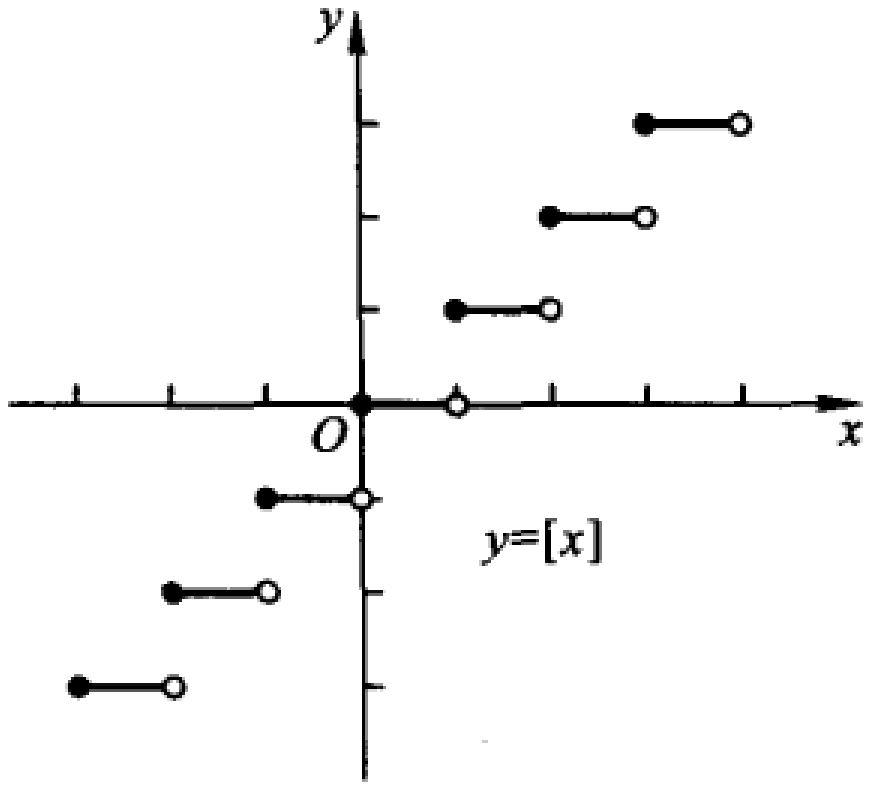
\includegraphics[width=0.72\textwidth]{work/figures/fig2-1}\figcap\label{fig:2-1}
\end{minipage}\hfill
\begin{minipage}[c]{0.48\textwidth}\centering
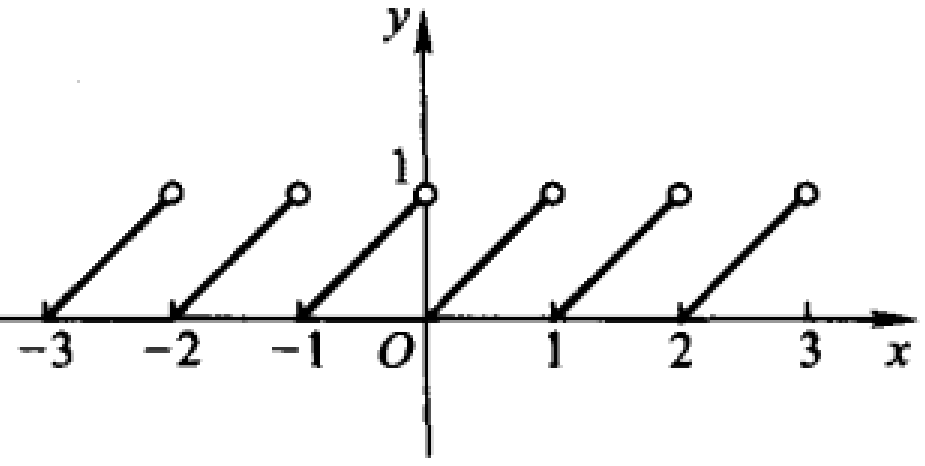
\includegraphics[width=0.72\textwidth]{work/figures/fig2-2}\figcap\label{fig:2-2}
\end{minipage}
\end{figure}

必须指出：函数 $f$ 是一种对应法则，它不是数，符号 $f\colon X\to\mathbb{R}$ 更明显地表示了这一点．然而符号 $y=f(x)$ 对每一个固定的 $x\in X$，它是一个数，是 $f$ 在 $x$ 处取的值．但如果理解 $x$ 可以取遍 $X$，那它也表示一个函数，而且它还有便于计算的优点．因此，以后大多采用这种记号．它既可表示函数，又可表示函数值．

\begin{example}\label{ex:2-1-2}
\[
f(x)=|x|=\begin{cases}
x, & x\geqslant0,\\
-x, & x<0.
\end{cases}
\]
\end{example}

\begin{figure}[htbp]
\centering
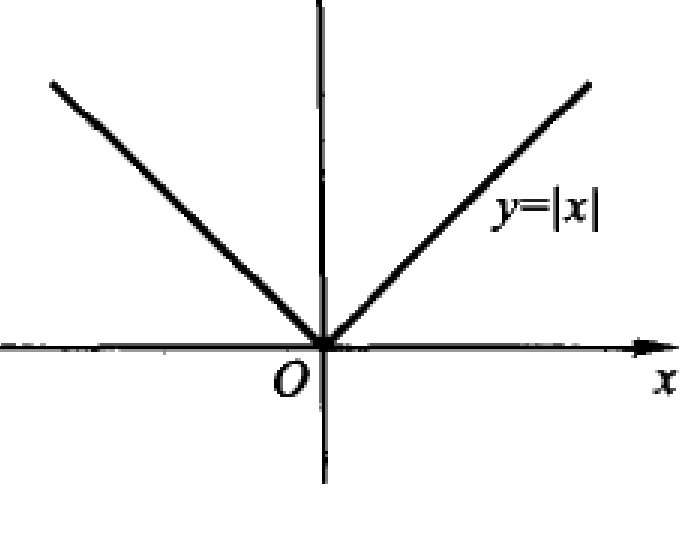
\includegraphics[width=0.36\textwidth]{work/figures/fig2-3}
\figcap\label{fig:2-3}
\end{figure}

这是定义在 $(-\infty,+\infty)$ 上的函数，它在定义域的不同部分分别由不同的表达式给出对应关系．这样定义的函数称为分段函数．注意这不是两个函数，而是一个函数，它给出的是一个对应法则．当 $x\geqslant0$ 时，由表达式 $x$ 确定对应关系；而当 $x<0$ 时，由表达式 $-x$ 确定对应关系．其图形如图~\ref{fig:2-3} 所示．

\begin{example}\label{ex:2-1-3}
\[
D(x)=\begin{cases}
1, & x\text{ 是有理数},\\
0, & x\text{ 是无理数}.
\end{cases}
\]
这个函数称为狄利克雷（Dirichlet，1806---1859）函数．定义域 $X=\mathbb{R}$，值域 $f(X)=\{0,1\}$．此函数的自变量可以认为是连续量，而因变量则显然不是连续量．这个函数在数学史中起过重要作用，它帮助澄清过许多概念．显然这个函数的图形是无法画出来的．
\end{example}

\begin{example}\label{ex:2-1-4}
考虑直线 $y=ax$（$a>0$）与直线 $x=x_0$（$x_0>0$）以及 $x$ 轴所围成的三角形的面积 $s$，有
\[
s(x_0)=\frac{1}{2}ax_0^2.
\]
当 $x_0$ 在 $(0,+\infty)$ 中变动时，我们可以得到函数
\[
s(x)=\frac{1}{2}ax^2,\qquad x>0.
\]
\end{example}

\begin{figure}[htbp]
\centering
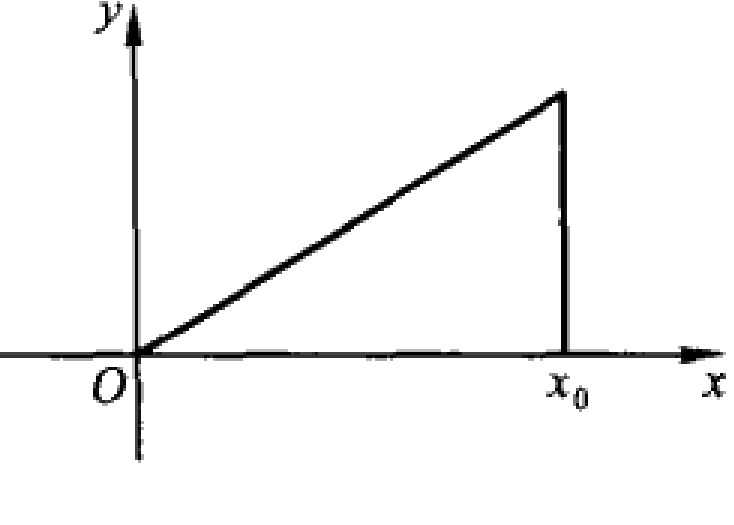
\includegraphics[width=0.38\textwidth]{work/figures/fig2-4}
\figcap\label{fig:2-4}
\end{figure}

这里定义域 $X=(0,+\infty)$ 是实际问题本身所决定的．而就表达式 $\frac{1}{2}ax^2$ 来说，对每一 $x\in(-\infty,+\infty)$，都可确定唯一的值．因此
\[
s(x)=\frac{1}{2}ax^2,\qquad x\in(-\infty,+\infty)
\]
也是一函数．$(-\infty,+\infty)$ 称为 $s(x)$ 的自然定义域，即使得该表达式有意义的所有 $x$ 构成的集合．以后写出一个函数表达式，如没有特别说明，自然就认为它的定义域是它的自然定义域．

\begin{example}\label{ex:2-1-5}
$y=\sqrt{\sin x}$．它表示一个函数，其定义域为 $2k\pi\leqslant x\leqslant (2k+1)\pi$，$k=0,\pm1,\pm2,\cdots$．
\end{example}

\begin{example}\label{ex:2-1-6}
常值函数 $f(x)=c$，$x\in X$．这是一个特殊的函数，对定义域内任一点，其函数值均为常数 $c$．
\end{example}

下面讨论函数的几种特性．

\subsection*{一、函数的奇偶性}

\begin{definition}\label{def:2-2}
设 $X$ 是关于原点对称的（即若 $x\in X$，则 $-x\in X$），$f$ 是定义在 $X$ 上的函数．若对任意 $x\in X$，有 $f(x)=-f(-x)$，则称 $f(x)$ 为奇函数；若对任意 $x\in X$，有 $f(x)=f(-x)$，则称 $f(x)$ 为偶函数．
\end{definition}

奇函数的图形特点是关于原点对称，而偶函数的图形特点是关于 $y$ 轴对称．例如，$y=x^3$ 是奇函数，而 $y=x^2$ 是偶函数，它们的图形分别如下：

\begin{figure}[htbp]
\centering
\begin{minipage}[c]{0.48\textwidth}\centering
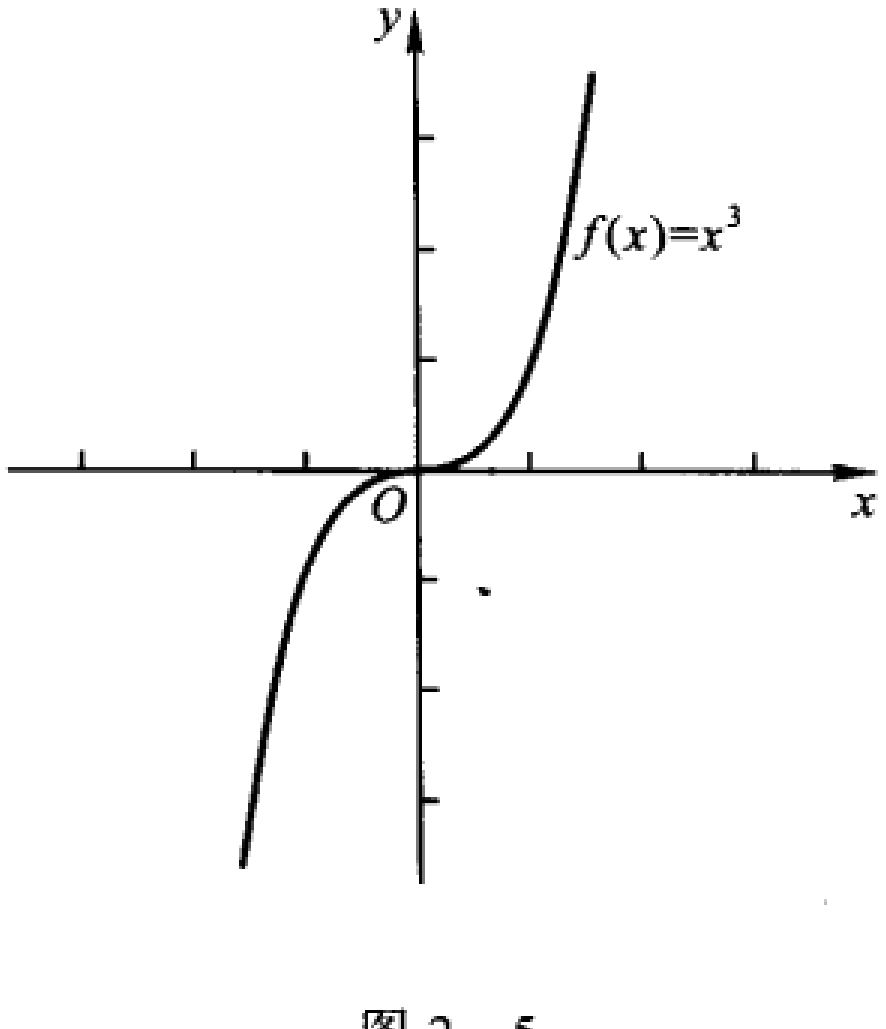
\includegraphics[width=0.72\textwidth]{work/figures/fig2-5}\figcap\label{fig:2-5}
\end{minipage}\hfill
\begin{minipage}[c]{0.48\textwidth}\centering
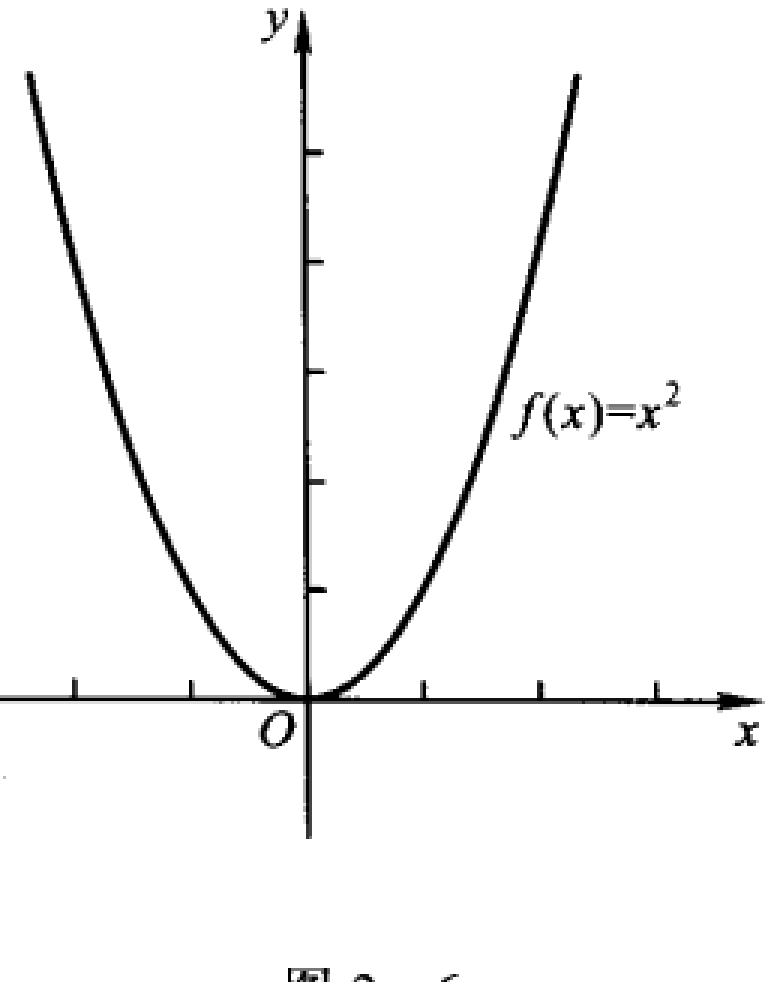
\includegraphics[width=0.72\textwidth]{work/figures/fig2-6}\figcap\label{fig:2-6}
\end{minipage}
\end{figure}

\subsection*{二、函数的单调性}

\begin{definition}\label{def:2-3}
设 $f(x)$ 是定义在 $X$ 上的函数．若对任意 $x_1,x_2\in X$，$x_1<x_2$，有 $f(x_1)\leqslant f(x_2)$，则称 $f(x)$ 在 $X$ 上单调上升或单调递增；若对任意 $x_1,x_2\in X$，$x_1<x_2$，有 $f(x_1)\geqslant f(x_2)$，则称 $f(x)$ 在 $X$ 上单调下降或单调递减．

当上述各不等号为严格不等时，分别称为严格单调上升和严格单调下降．单调上升和单调下降函数统称为单调函数．
\end{definition}

例如 $y=x^3$ 在 $(-\infty,+\infty)$ 是严格单调上升的；$y=x^2$ 在 $(-\infty,0)$ 严格单调下降，而在 $(0,+\infty)$ 是严格单调上升的，但在 $(-\infty,+\infty)$ 不是单调的．又 $y=[x]$ 在 $(-\infty,+\infty)$ 是单调上升，但非严格单调上升．

\subsection*{三、函数的周期性}

\begin{definition}\label{def:2-4}
设函数 $f(x)$ 在 $X$ 上有定义．若存在正数 $T>0$，对任意 $x\in X$，有 $x+T\in X$，且 $f(x+T)=f(x)$，则称 $f(x)$ 是周期函数，$T$ 称为 $f(x)$ 的周期．
\end{definition}

显然，若 $T$ 是 $f(x)$ 的周期，则 $2T,3T,\cdots$ 都是 $f(x)$ 的周期．通常函数的周期是指它的最小周期（如果存在的话）．

例如，$y=\sin x$ 的周期是 $2\pi$；$y=|\sin x|$ 的周期为 $\pi$．但并不是所有周期函数都有最小周期．例如，狄利克雷函数
\[
D(x)=\begin{cases}
1, & x\text{ 是有理数},\\
0, & x\text{ 是无理数}.
\end{cases}
\]
因为任意正有理数都是它的周期，而正有理数是没有最小（正有理）数的．

周期函数的图形可将一个周期上的图形逐段平移而得到．也就是说只要知道了函数在一个周期上的图形，便可作出整个函数的图形．

\subsection*{四、函数的有界性}

\begin{definition}\label{def:2-5}
设 $f(x)$ 在 $X$ 上有定义．若存在 $M>0$，对任意 $x\in X$，有
\[
|f(x)|\leqslant M,
\]
则称 $f(x)$ 在 $X$ 上有界．
\end{definition}

注意，上式又等价于
\[
-M\leqslant f(x)\leqslant M,\qquad x\in X.
\]
在几何上，它表示函数 $f(x)$ 的图形完全位于直线 $y=-M$ 和 $y=M$ 之间．例如，$y=x-[x]$ 在 $(-\infty,+\infty)$ 是有界的，因为存在 $M=1$，使得
\[
|x-[x]|\leqslant 1,\qquad x\in(-\infty,+\infty).
\]
事实上从函数的图形明显可知，$0\leqslant x-[x]<1$（参见图~\ref{fig:2-2}）．

\begin{proposition}\label{prop:2-1}
$f(x)$ 在 $X$ 上有界的充要条件是存在 $A,B$，使得
\[
A\leqslant f(x)\leqslant B,\qquad x\in X.
\]
\end{proposition}

\begin{proof}
必要性：已知 $f(x)$ 有界，即
\[
|f(x)|\leqslant M,\qquad x\in X,
\]
它等价于
\[
-M\leqslant f(x)\leqslant M,\qquad x\in X.
\]
取 $A=-M$，$B=M$，必要性获证．

充分性：已知
\[
A\leqslant f(x)\leqslant B,\qquad x\in X,
\]
取 $M=\max(|A|,|B|)$，则
\[
\begin{aligned}
f(x) &\leqslant B\leqslant |B|\leqslant M,\\
-f(x) &\leqslant -A\leqslant |A|\leqslant M,
\end{aligned}
\]
即
\[
|f(x)|\leqslant M,\qquad x\in X.
\]
充分性获证，从而命题证完．
\end{proof}

这个命题很简单，但即使是这样简单的命题的证明，我们也要求读者能把它写清楚．

通常称命题中的 $A$ 为 $f(x)$ 在 $X$ 上的下界，称 $B$ 为 $f(x)$ 在 $X$ 上的上界．命题~\ref{prop:2-1} 说的是，$f(x)$ 在 $X$ 有界的充要条件是它有上界且有下界．

$f(x)$ 在 $X$ 上无界与 $f(x)$ 在 $X$ 上有界是互相排斥的，两者必居其一．因此，$f(x)$ 在 $X$ 上无界，即是说不存在 $M>0$，使得对所有的 $x\in X$，都满足 $|f(x)|\leqslant M$．但是这样的说法不易验证，为此，我们从正面来叙述，或用肯定的语气来叙述为：对任意 $M>0$，都存在 $x_0\in X$，使得 $|f(x_0)|>M$．

\begin{example}\label{ex:2-1-7}
证明 $f(x)=\frac{1}{x}$ 在 $(0,1)$ 内无界．
\end{example}

\begin{proof}
对任意 $M>0$，取 $x_0=\frac{1}{M+1}\in(0,1)$，则
\[
|f(x_0)|=f(x_0)=\frac{1}{x_0}=M+1>M.
\]
故 $f(x)=\frac{1}{x}$ 在 $(0,1)$ 内无界．
\end{proof}

读者不妨考虑一下，如果不用无界的这种“肯定语气”，这个题目怎样做？

\begin{xiti}
\item 证明下列不等式：
  \begin{ziti}
  \item $|x-y|\geqslant\bigl||x|-|y|\bigr|$；
  \item $|x_1+x_2+\cdots+x_n|\leqslant|x_1|+|x_2|+\cdots+|x_n|$；
  \item $|x_1+x_2+\cdots+x_n+x|\geqslant|x|-(|x_1|+|x_2|+\cdots+|x_n|)$．
  \end{ziti}
\item 求证 $\dfrac{|a+b|}{1+|a+b|}\leqslant\dfrac{|a|}{1+|a|}+\dfrac{|b|}{1+|b|}$．
\item 求证
\[
\max(a,b)=\frac{a+b}{2}+\frac{|a-b|}{2};\qquad \min(a,b)=\frac{a+b}{2}-\frac{|a-b|}{2}.
\]
\item 已知三角形的两条边分别为 $a$ 和 $b$，它们之间的夹角为 $\theta$，试求此三角形的面积 $s(\theta)$，并求其定义域．
\item 在半径为 $r$ 的球内嵌入一内接圆柱，试将圆柱的体积表为其高的函数，并求此函数的定义域．
\item 某公共汽车路线全长为 $20\,\mathrm{km}$，票价规定如下：乘坐 $5\,\mathrm{km}$ 以下（包括 $5\,\mathrm{km}$）者收费 $1$ 元；超过 $5\,\mathrm{km}$ 但在 $15\,\mathrm{km}$ 以下（包括 $15\,\mathrm{km}$）者收费 $2$ 元；其余收费 $2$ 元 $5$ 角．试将票价表为路程的函数，并作出函数的图形．
\item 一脉冲发生器产生一个三角波．若记它随时间 $t$ 的变化规律为 $f(t)$，且三个角分别有对应关系 $f(0)=0$，$f(10)=20$，$f(20)=0$，求 $f(t)$（$0\leqslant t\leqslant 20$），并作出函数的图形．
\item 判别下列函数的奇偶性：
  \begin{ziti}
  \item $f(x)=\dfrac{x^4}{2}+x^2-1$；
  \item $f(x)=x+\sin x$；
  \item $f(x)=x^2\mathrm{e}^{-x^2}$；
  \item $f(x)=\lg(x+\sqrt{1+x^2})$．
  \end{ziti}
\item 判别下列函数是否是周期函数，若是，试求其周期：
  \begin{ziti}
  \item $f(x)=\cos x^2$；
  \item $f(x)=\cos\dfrac{x}{2}+2\sin\dfrac{x}{3}$；
  \item $f(x)=\cos\dfrac{\pi}{4}x$；
  \item $f(x)=\sqrt{\tan x}$．
  \end{ziti}
\item 证明 $f(x)=\dfrac{x}{x^2+1}$ 在 $(-\infty,+\infty)$ 有界．
\item 用肯定语气叙述函数 $f(x)$ 在 $(a,b)$ 无界，并证明 $f(x)=\dfrac{1}{x^2}$ 在 $(0,1)$ 无界．
\item 试证两个偶函数的乘积是偶函数，两个奇函数的乘积是偶函数，一个奇函数与一个偶函数的乘积是奇函数．
\item 设 $f(x)$ 为定义在 $(-\infty,+\infty)$ 内的任何函数，证明 $f(x)$ 可分解成奇函数与偶函数之和．
\item 用肯定语气叙述：在 $(-\infty,+\infty)$ 上
  \begin{ziti}
  \item $f(x)$ 不是奇函数；
  \item $f(x)$ 不是单调上升函数；
  \item $f(x)$ 无零点；
  \item $f(x)$ 无上界．
  \end{ziti}
\end{xiti}

\section{复合函数与反函数}\label{sec:2.2}

有了函数的概念后，我们来讨论函数的运算，这样就可以从几个最简单的函数出发，通过运算来获得更多、更复杂的函数．函数的加、减、乘、除四则运算是大家已经熟知的了，本节主要讨论函数的复合运算和取反函数运算．

\subsection*{1. 复合函数}

我们已经知道自由落体运动中，速度 $v$ 与时间 $t$ 的关系是
\[
v=gt,
\]
而质点的动能为 $M=\frac{1}{2}mv^2$，这样动能依赖于时间的变化关系为
\[
M=\frac{1}{2}mv^2,\qquad v=gt,
\]
或
\[
M=\frac{1}{2}mg^2t^2.
\]
可见 $v$ 在这里起的是桥梁作用．我们称它为中间变量，通过中间变量架起的桥梁，将两个函数复合为一个函数．

\begin{definition}\label{def:2-6}
设函数 $y=f(u)$ 的定义域为 $U$，$u=g(x)$ 的定义域为 $X$，且 $g(X)\subset U$，则 $y=f(g(x))$ 是定义在 $X$ 上的函数，称为 $f$ 与 $g$ 的复合函数，有时也记为 $f\circ g$．$u$ 称为中间变量．
\end{definition}

定义中条件 $g(X)\subset U$ 保证了 $f\circ g$ 确实能给出一个对应法则．这时对每一个 $x\in X$，都有 $g(x)\in U$．而 $f$ 是定义在 $U$ 上的函数，因而有唯一的 $y$ 与 $g(x)$ 对应，也就是说有唯一的 $y$ 与 $x$ 对应．这样就建立了 $X$ 上的对应法则 $f\circ g$．更一般地，若 $g(X)\cap U\neq\emptyset$，仍可得到复合函数 $f\circ g$，但这时复合函数的定义域不是 $X$，而是 $X$ 的一个子集 $X_1=\{x\in X\mid g(x)\in U\}$．可见并不是任意两个函数都可进行复合而成为复合函数，关键在于它们的复合是否确能给出一个对应法则．例如，$u=g(x)=1+a^x$，$y=f(u)=\sqrt{1-u^2}$，显然函数 $f$ 的定义域为 $[-1,1]$，而 $g(x)>1$，因此不可能通过 $u$ 复合为函数．

\begin{example}\label{ex:2-2-1}
设
\[
f(x)=\begin{cases}
x+1, & x>1,\\
x^2, & x\leqslant1,
\end{cases}\qquad g(x)=5x+3.
\]
求 $f(g(x))$ 和 $g(f(x))$．
\end{example}

\begin{proof}[解]
$f(x)$ 和 $g(x)$ 的定义域都是 $(-\infty,+\infty)$，所以存在复合函数 $f(g(x))$ 和 $g(f(x))$．又 $5x+3>1$ 当且仅当 $x>-\frac{2}{5}$，故有
\[
f(g(x))=\begin{cases}
5x+4, & x>-\frac{2}{5},\\
(5x+3)^2, & x\leqslant-\frac{2}{5},
\end{cases}
\]
\[
g(f(x))=\begin{cases}
5(x+1)+3, & x>1,\\
5x^2+3, & x\leqslant1.
\end{cases}
\]
\end{proof}

从上述例子可见，一般说来，复合运算并不满足交换律，即 $f\circ g\neq g\circ f$．

\subsection*{2. 反函数}

在匀速直线运动中，有关系式 $s=vt$，这里时间 $t$ 是自变量，路程 $s$ 是因变量，由时间可计算出路程．但也会出现这样的情形，即已测得路程 $s$，要求推算时间 $t$，也就是说要求把 $s$ 作为自变量，$t$ 作为因变量．可见自变量与因变量往往是相对的．那么什么情况下可以使自变量与因变量相互转化呢？这就是反函数的概念．

\begin{definition}\label{def:2-7}
设 $y=f(x)$ 是定义在 $X$ 上的函数．如果对值域 $f(X)$ 的每个 $y$，都有唯一的 $x\in X$，使得 $f(x)=y$，则这样定义的 $x$ 作为 $y$ 的函数，称为 $f$ 的反函数，记为 $f^{-1}$，即
\[
f^{-1}\colon y\to x,\qquad \text{如果 } y=f(x).
\]
\end{definition}

并不是所有的函数都有反函数存在．例如，$y=x^2$，$x\in(-\infty,+\infty)$．对每个 $y>0$，与之对应的 $x$ 不唯一，因为有两个值 $x=\pm\sqrt{y}$ 满足 $y=x^2$，因此不能确定从 $(0,+\infty)$ 到 $\mathbb{R}$ 的对应关系．很容易看出，反函数存在的条件是：对任意 $x_1,x_2\in X$，$x_1\neq x_2$，有 $f(x_1)\neq f(x_2)$．也就是说，$f$ 在 $X$ 与 $f(X)$ 之间建立的是一个一一对应的关系．由此得到，若 $f(x)$ 在 $X$ 严格单调，则它一定有反函数存在．显然，如果函数 $f$ 有反函数 $f^{-1}$ 存在，那么
\[
f^{-1}(f(x))=x,\quad \forall x\in X,
\]
\[
f(f^{-1}(y))=y,\quad \forall y\in f(X),
\]
其中“$\forall$”是逻辑符号，意指“对任意”．

函数与反函数，是对应关系为互逆，用什么字母表示是不重要的，但通常我们习惯于用 $x$ 表示自变量，用 $y$ 表示因变量．因此 $y=f(x)$，$x\in X$ 的反函数仍写为
\[
y=f^{-1}(x),\qquad x\in f(X).
\]
它与
\[
x=f^{-1}(y),\qquad y\in f(X)
\]
是同一函数，因为对应法则都是 $f^{-1}$，定义域也都是 $f$ 的值域 $f(X)$．

\begin{example}\label{ex:2-2-2}
函数 $y=x^2$，$x\in(0,+\infty)$ 的反函数为
\[
x=\sqrt{y},\qquad y\in(0,+\infty),
\]
或
\[
y=\sqrt{x},\qquad x\in(0,+\infty).
\]
其图形如图~\ref{fig:2-7} 所示．
\end{example}

\begin{figure}[htbp]
\centering
\begin{minipage}[c]{0.48\textwidth}\centering
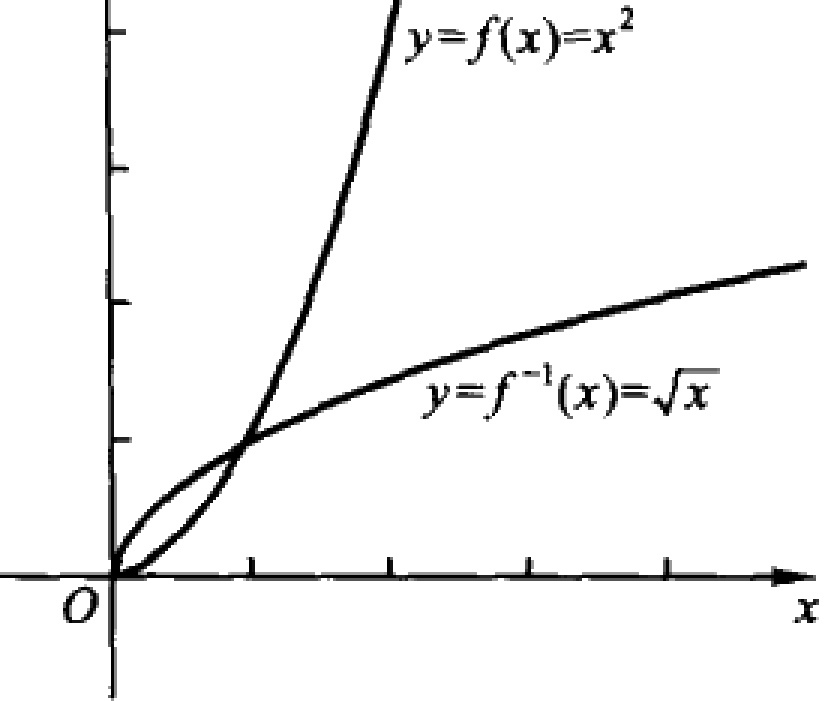
\includegraphics[width=0.72\textwidth]{work/figures/fig2-7}\figcap\label{fig:2-7}
\end{minipage}\hfill
\begin{minipage}[c]{0.48\textwidth}\centering
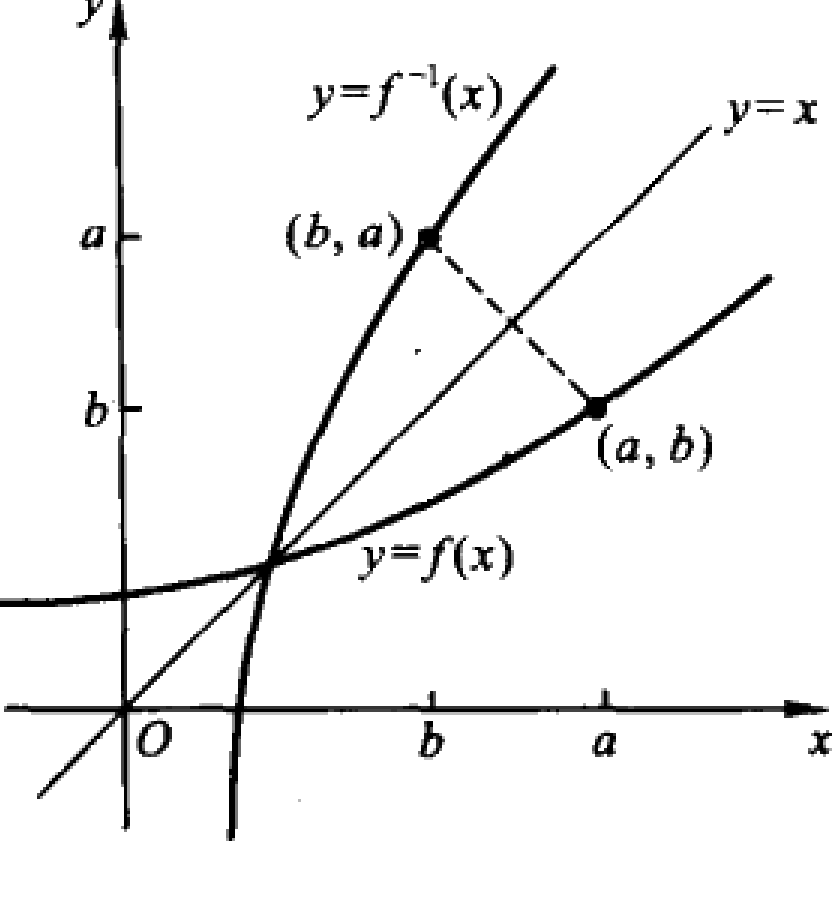
\includegraphics[width=0.72\textwidth]{work/figures/fig2-8}\figcap\label{fig:2-8}
\end{minipage}
\end{figure}

在作函数的图形时，我们也往往习惯于用横坐标表示自变量，用纵坐标表示因变量．这时 $y=f^{-1}(x)$ 的图形与 $y=f(x)$ 的图形有什么关系呢？若 $(a,b)$ 在曲线 $y=f(x)$ 上，由反函数的定义知，$(b,a)$ 必在曲线 $y=f^{-1}(x)$ 上．而 $(b,a)$ 与 $(a,b)$ 是关于直线 $y=x$ 对称的点．因此 $y=f^{-1}(x)$ 的图形与 $y=f(x)$ 的图形是关于直线 $y=x$ 对称的（见图~\ref{fig:2-8}）．这样，由 $y=f(x)$ 的图形便很容易作出 $y=f^{-1}(x)$ 的图形．

\begin{proposition}\label{prop:2-2}
严格递增（减）的函数必有反函数，且其反函数也是严格递增（减）的．
\end{proposition}

\begin{proof}
反函数存在性是显然的（前面已说过）．设 $f(x)$ 在 $X$ 严格递增，要证 $f^{-1}(y)$ 在 $f(X)$ 也是严格递增的．用反证法．如果不然，存在 $y_1,y_2\in f(X)$，$y_1<y_2$，但 $f^{-1}(y_1)\geqslant f^{-1}(y_2)$，这时 $f(f^{-1}(y_1))\geqslant f(f^{-1}(y_2))$，即 $y_1\geqslant y_2$，矛盾．命题~\ref{prop:2-2} 证完．
\end{proof}

\begin{xiti}
\item 设 $f(x)=\dfrac{1-x}{1+x}$，求证 $f(f(x))=x$．
\item 求下列函数的反函数及其定义域：
  \begin{ziti}
  \item $y=\dfrac{1}{2}\left(x+\dfrac{1}{x}\right)$,\quad $1<x<+\infty$；
  \item $y=\dfrac{1}{2}(\mathrm{e}^x-\mathrm{e}^{-x})$,\quad $-\infty<x<+\infty$；
  \item $y=\begin{cases}
  x, & -\infty<x<1,\\
  x^2, & 1\leqslant x\leqslant 4,\\
  2^x, & 4<x<+\infty.
  \end{cases}$
  \end{ziti}
\item 设 $f(x)$，$g(x)$ 为实轴上单调函数，求证 $f(g(x))$ 也是实轴上的单调函数．
\item 设
\[
f(x)=\begin{cases}
-x-1, & x\leqslant0,\\
x, & x>0,
\end{cases}\qquad g(x)=\begin{cases}
x, & x\leqslant0,\\
-x^2, & x>0.
\end{cases}
\]
求复合函数 $f(g(x)), g(f(x))$．
\item 设 $f(x)=\dfrac{x}{\sqrt{1+x^2}}$，求 $(f\underbrace{\circ f\circ\cdots\circ f}_{n\text{ 次}})(x)$．
\item 设 $f(x)=|1+x|-|1-x|$，试求 $(f\underbrace{\circ f\circ\cdots\circ f}_{n\text{ 次}})(x)$．
\item 设 $f(x)=\dfrac{1}{1-x}$，求 $f(f(x))$，$f(f(f(x)))$，$f\left(\dfrac{1}{f(x)}\right)$．
\end{xiti}

\section{初等函数}\label{sec:2.3}

有了函数的四则运算和复合运算，我们可以从六种函数出发，通过运算来获得更多的函数，这六种函数是常值函数，指数函数，幂函数，对数函数，三角函数和反三角函数．称它们为基本初等函数．

函数若是由基本初等函数经有限次的四则运算和复合所得到，则称为初等函数．否则，称为非初等函数．因此，首先必须熟悉基本初等函数的性质及其图形．

\subsection*{(1) 常值函数}
\[
y=c,\qquad x\in(-\infty,+\infty)
\]
在本章§\ref{sec:2.1}例~\ref{ex:2-1-6}已介绍过．

\subsection*{(2) 指数函数}
\[
y=a^x,\qquad x\in(-\infty,+\infty)\quad(a>0,a\neq1).
\]
函数的值域是 $(0,+\infty)$，图形总经过点 $(0,1)$．当 $a>1$ 时，函数严格单调上升；当 $0<a<1$ 时，函数严格单调下降．$a^x$ 与 $\left(\frac{1}{a}\right)^x$ 的图形关于 $y$ 轴对称（见图~\ref{fig:2-9}）．

\subsection*{(3) 对数函数}
\[
y=\log_a x,\qquad x\in(0,+\infty)\quad(a>0,a\neq1).
\]
对数函数与指数函数互为反函数．因此由指数函数的性质立即知，对数函数的值域是 $(-\infty,+\infty)$，图形总经过点 $(1,0)$，当 $a>1$ 时，函数严格单调上升；当 $0<a<1$ 时，函数严格单调下降．$\log_a x$ 与 $\log_{\frac{1}{a}}x$ 的图形关于 $x$ 轴对称（见图~\ref{fig:2-10}）．

\begin{figure}[htbp]
\centering
\begin{minipage}[c]{0.48\textwidth}\centering
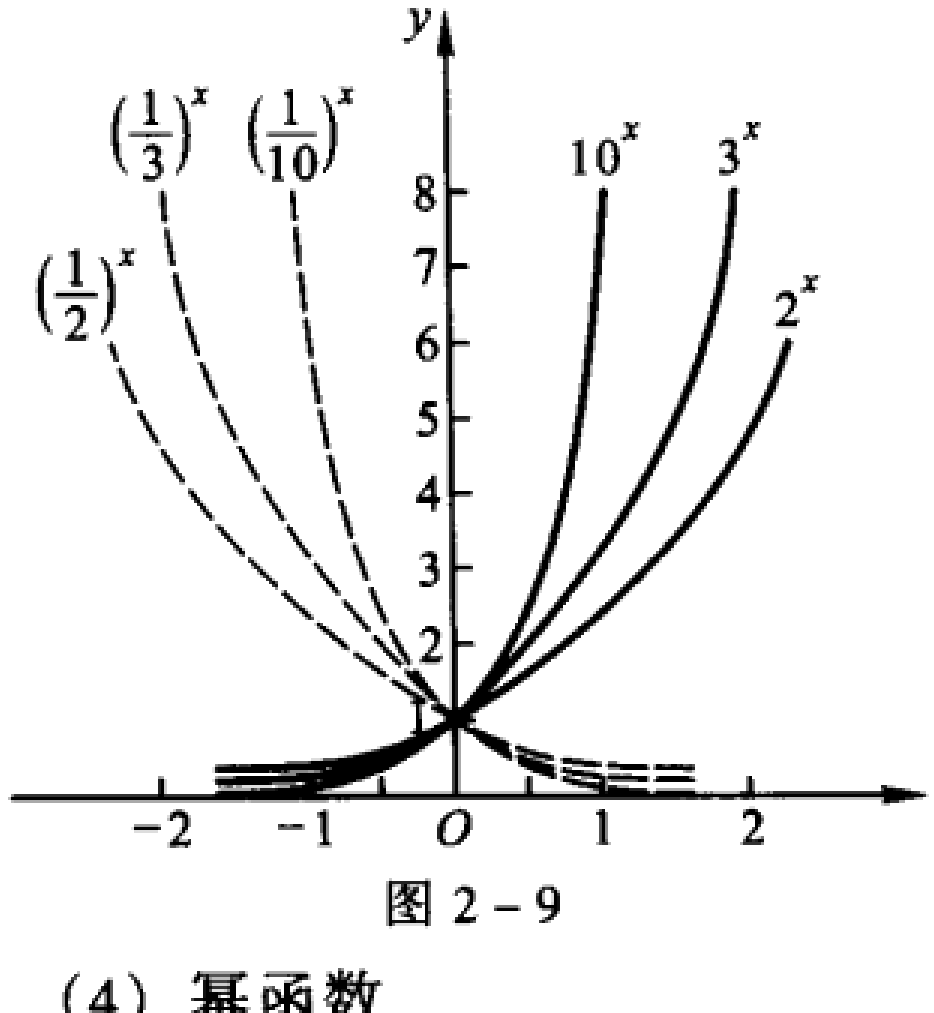
\includegraphics[width=0.72\textwidth]{work/figures/fig2-9}\figcap\label{fig:2-9}
\end{minipage}\hfill
\begin{minipage}[c]{0.48\textwidth}\centering
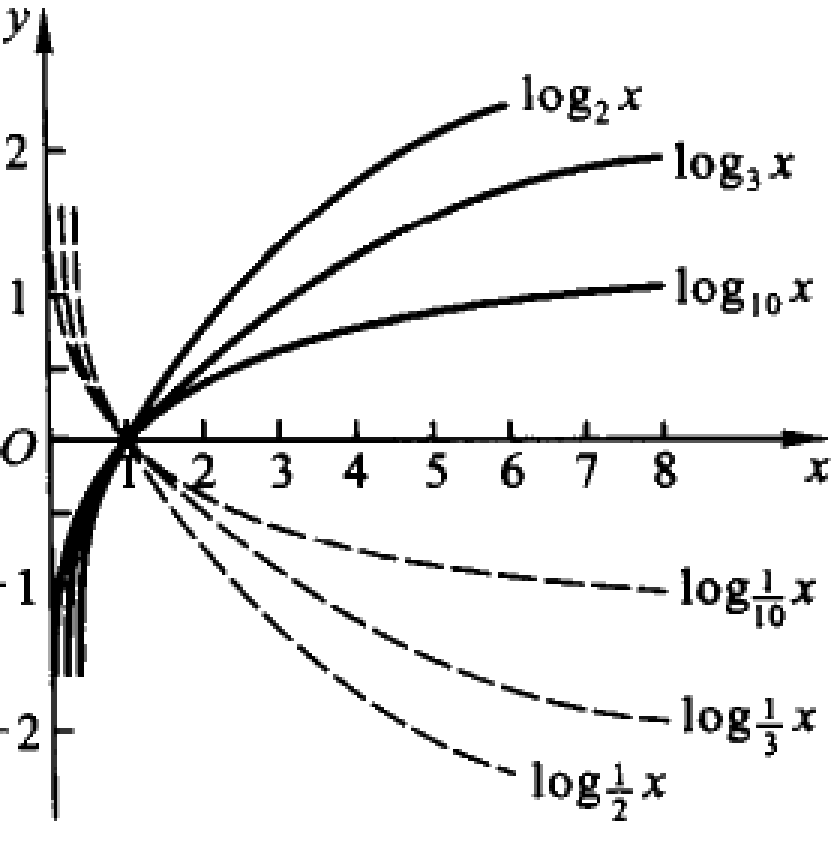
\includegraphics[width=0.72\textwidth]{work/figures/fig2-10}\figcap\label{fig:2-10}
\end{minipage}
\end{figure}

\subsection*{(4) 幂函数}
\[
y=x^{\mu},\qquad \text{其中 }\mu\neq0.
\]
幂函数的定义域根据 $\mu$ 值的不同而不同．当 $\mu=\frac{p}{q}$ 是有理数时（其中 $p,q$ 是整数，且 $p,q$ 互素），其定义域见下表：

\begin{table}[htbp]
\centering
\begin{tabular}{|c|c|c|}
\hline
\multicolumn{2}{|c|}{$\mu = \frac{p}{q}$} & 定义域 \\
\hline
\multirow{2}{*}{$\mu > 0$} & $q$ 为奇数 & $(-\infty, +\infty)$ \\
\cline{2-3}
 & $q$ 为偶数 & $[0, +\infty)$ \\
\hline
\multirow{2}{*}{$\mu < 0$} & $q$ 为奇数 & $(-\infty, 0) \cup (0, +\infty)$ \\
\cline{2-3}
 & $q$ 为偶数 & $(0, +\infty)$ \\
\hline
\end{tabular}
\end{table}

当 $\mu$ 是无理数时，$x^{\mu}$ 定义为 $x^{\mu}=10^{\mu\lg x}$，故定义域为 $(0,+\infty)$．可见不论 $\mu\,(\neq0)$ 为何值，幂函数 $x^{\mu}$ 在 $(0,+\infty)$ 总有定义．

当 $x>0$ 时，$x^{\mu}>0$，故此时函数的图形在第一象限，函数的图形总经过点 $(1,1)$，当 $\mu>0$ 时，函数严格单调上升；当 $\mu<0$ 时，函数严格单调下降．函数 $x^{\mu}$ 和 $x^{\frac{1}{\mu}}$ 互为反函数，图形关于直线 $y=x$ 对称（见图~\ref{fig:2-11} 和图~\ref{fig:2-12}）．

\begin{figure}[htbp]
\centering
\begin{minipage}[c]{0.48\textwidth}\centering
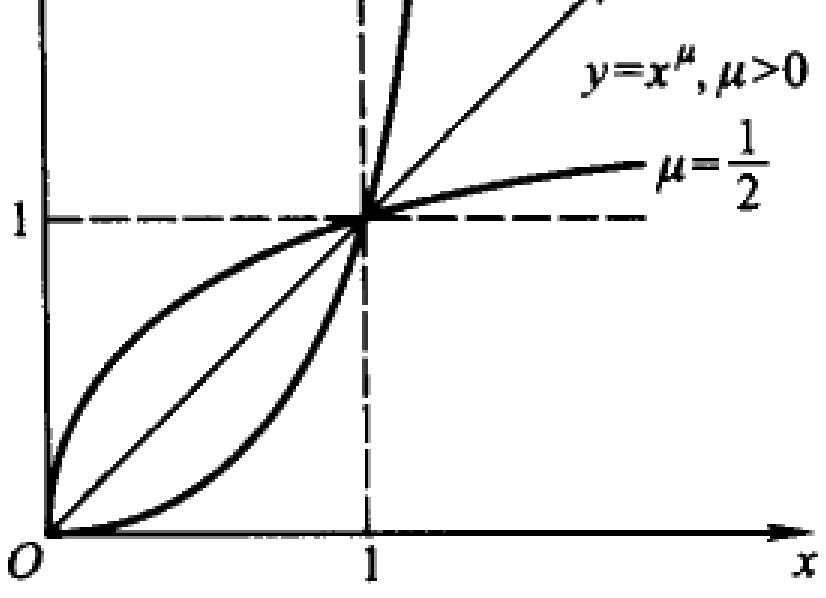
\includegraphics[width=0.72\textwidth]{work/figures/fig2-11}\figcap\label{fig:2-11}
\end{minipage}\hfill
\begin{minipage}[c]{0.48\textwidth}\centering
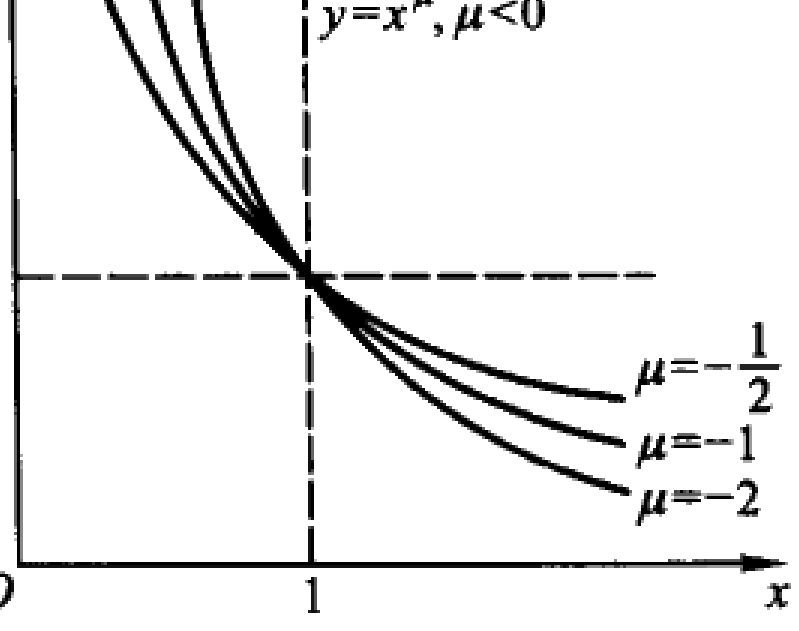
\includegraphics[width=0.72\textwidth]{work/figures/fig2-12}\figcap\label{fig:2-12}
\end{minipage}
\end{figure}

\subsection*{(5) 三角函数}

正弦函数 $y=\sin x$，$x\in(-\infty,+\infty)$；

余弦函数 $y=\cos x$，$x\in(-\infty,+\infty)$；

正切函数 $y=\tan x$，$x\neq k\pi+\frac{\pi}{2}$，$k=0,\pm1,\pm2,\cdots$；

余切函数 $y=\cot x$，$x\neq k\pi$，$k=0,\pm1,\pm2,\cdots$．

这些函数都是周期函数．正弦和余弦函数的周期为 $2\pi$，值域为 $[-1,1]$．正切和余切函数的周期为 $\pi$，值域为 $(-\infty,+\infty)$，它们的图形如图~\ref{fig:2-13} 和图~\ref{fig:2-14} 所示．

注意，在微积分中，三角函数的自变量 $x$ 一般是用弧度．

\begin{figure}[htbp]
\centering
\begin{minipage}[c]{0.48\textwidth}\centering
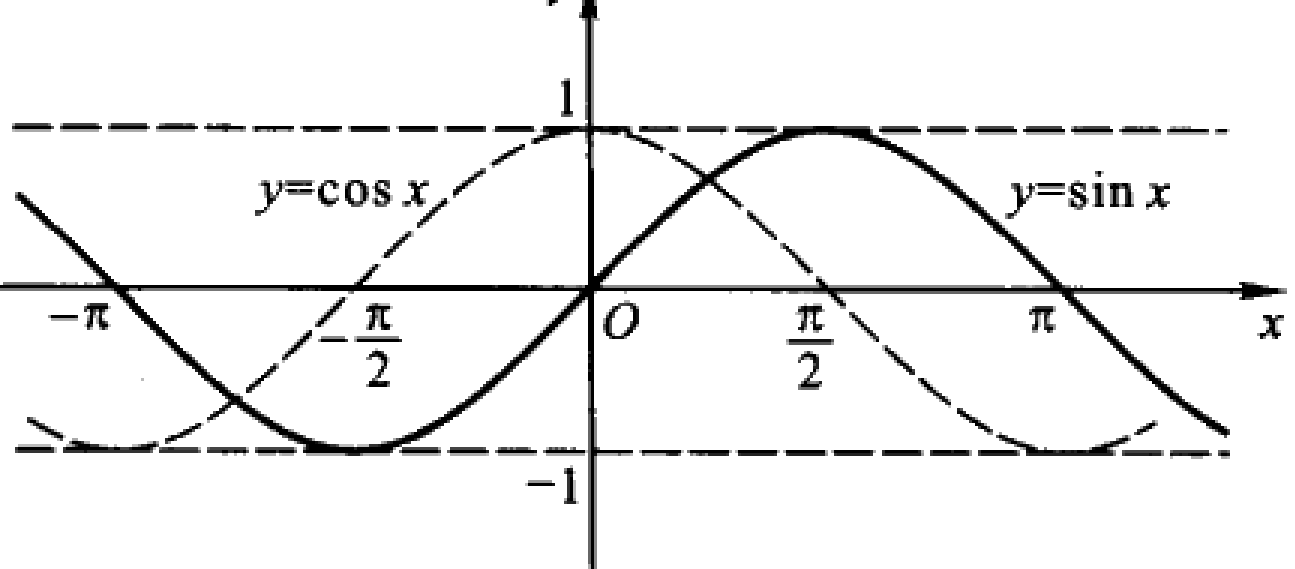
\includegraphics[width=0.78\textwidth]{work/figures/fig2-13}\figcap\label{fig:2-13}
\end{minipage}\hfill
\begin{minipage}[c]{0.48\textwidth}\centering
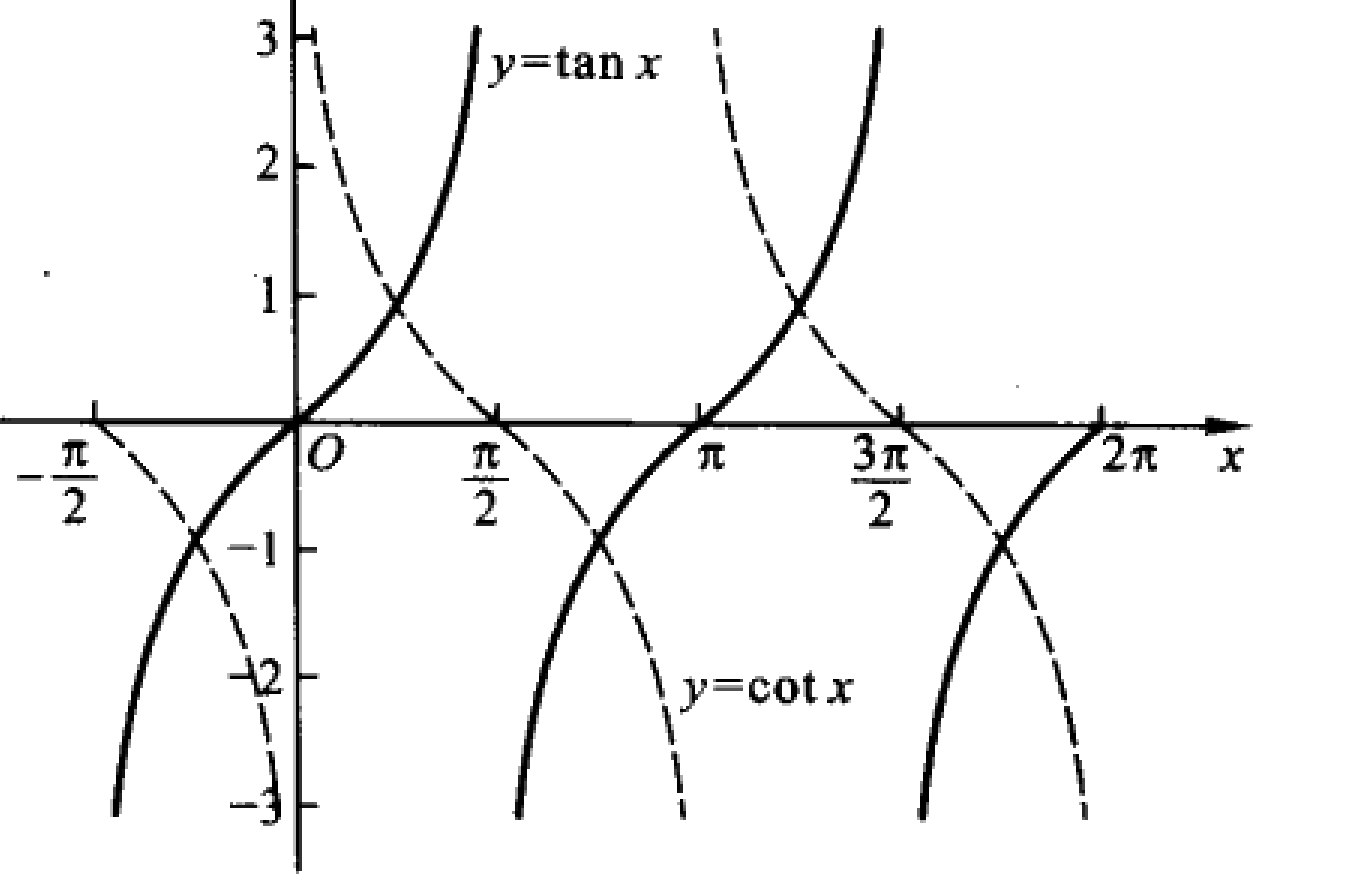
\includegraphics[width=0.78\textwidth]{work/figures/fig2-14}\figcap\label{fig:2-14}
\end{minipage}
\end{figure}

\subsection*{(6) 反三角函数}

因为三角函数不是一一对应的，因此我们只能分别在它们的一个严格单调分支上来讨论反函数．

反正弦函数 $y=\arcsin x$，$x\in[-1,1]$，$y\in\left[-\frac{\pi}{2},\frac{\pi}{2}\right]$；

反余弦函数 $y=\arccos x$，$x\in[-1,1]$，$y\in[0,\pi]$；

反正切函数 $y=\arctan x$，$x\in(-\infty,+\infty)$，$y\in\left(-\frac{\pi}{2},\frac{\pi}{2}\right)$；

反余切函数 $y=\operatorname{arccot} x$，$x\in(-\infty,+\infty)$，$y\in(0,\pi)$．

反正弦和反正切函数在定义域内严格单调上升且是奇函数，而反余弦和反余切函数在定义域内严格单调下降．它们的图形分别见图~\ref{fig:2-15}～图~\ref{fig:2-18}．

\begin{figure}[htbp]
\centering
\begin{minipage}[c]{0.48\textwidth}\centering
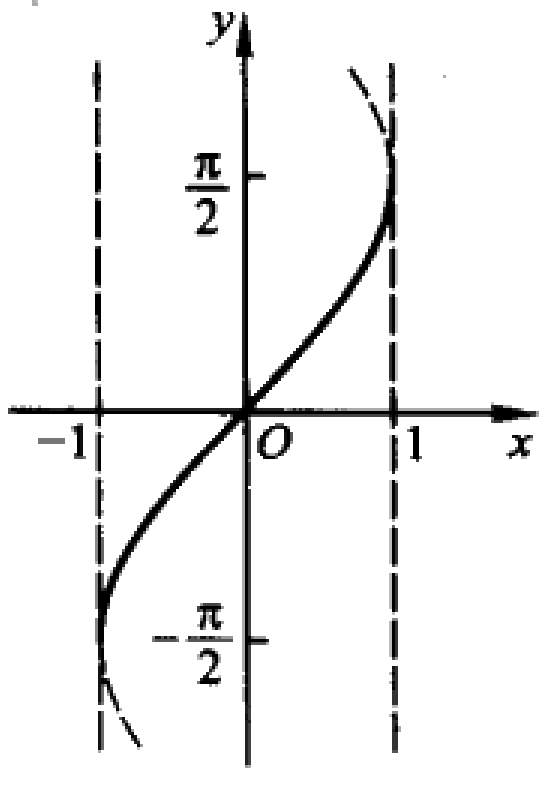
\includegraphics[width=0.70\textwidth]{work/figures/fig2-15}\figcap\label{fig:2-15}
\end{minipage}\hfill
\begin{minipage}[c]{0.48\textwidth}\centering
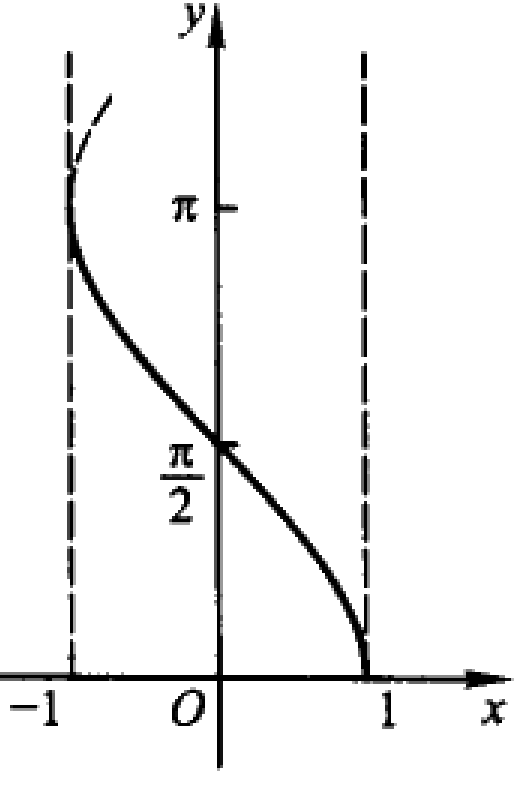
\includegraphics[width=0.70\textwidth]{work/figures/fig2-16}\figcap\label{fig:2-16}
\end{minipage}\\[1em]
\begin{minipage}[c]{0.48\textwidth}\centering
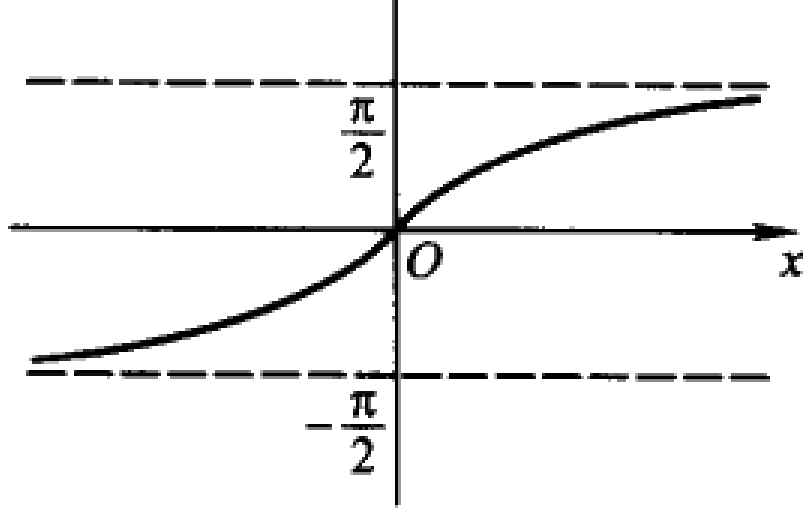
\includegraphics[width=0.70\textwidth]{work/figures/fig2-17}\figcap\label{fig:2-17}
\end{minipage}\hfill
\begin{minipage}[c]{0.48\textwidth}\centering
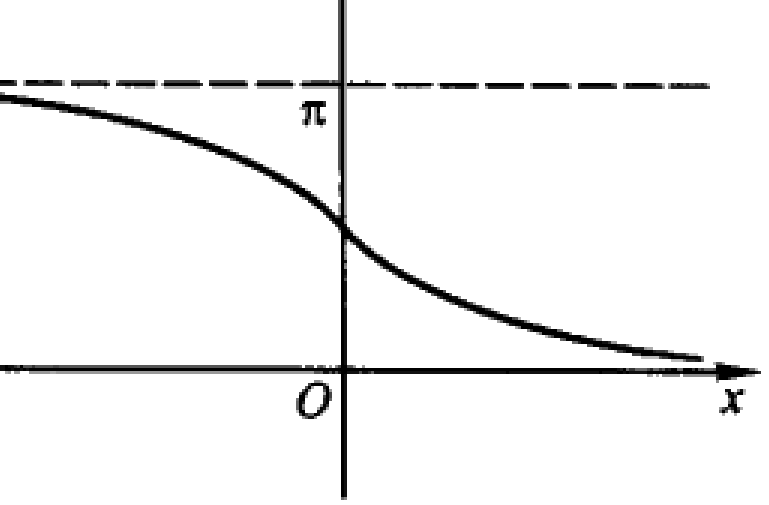
\includegraphics[width=0.70\textwidth]{work/figures/fig2-18}\figcap\label{fig:2-18}
\end{minipage}
\end{figure}

\begin{example}\label{ex:2-3-1}
$y=\arctan 2^{-x}$ 是初等函数，定义域是 $(-\infty,+\infty)$，值域是 $\left(0,\frac{\pi}{2}\right)$．函数在定义域内是严格单调下降的，这是因为 $2^{-x}=\left(\frac{1}{2}\right)^x$ 是严格单调下降的，而 $\arctan x$ 是严格单调上升的．
\end{example}

\begin{example}\label{ex:2-3-2}
作出函数 $y=\sin(2x+\pi)$ 的图形．
\end{example}

\begin{proof}[解]
\[
\sin[2(x+\pi)+\pi]=\sin(2x+\pi)=-\sin 2x,
\]
故函数是以 $\pi$ 为周期的周期函数．先作 $\sin 2x$ 的图形，然后将图形绕 $x$ 轴旋转 $180^\circ$，即得所要作的函数图形（图~\ref{fig:2-19}）．
\end{proof}

\begin{example}\label{ex:2-3-3}
\[
y=\begin{cases}
\mathrm{e}^x, & x\geqslant0,\\
0, & x<0,
\end{cases}
\]
它在每个分段上都是初等函数，但它不是初等函数，这点以后可加以证明．
\end{example}

\begin{figure}[htbp]
\centering
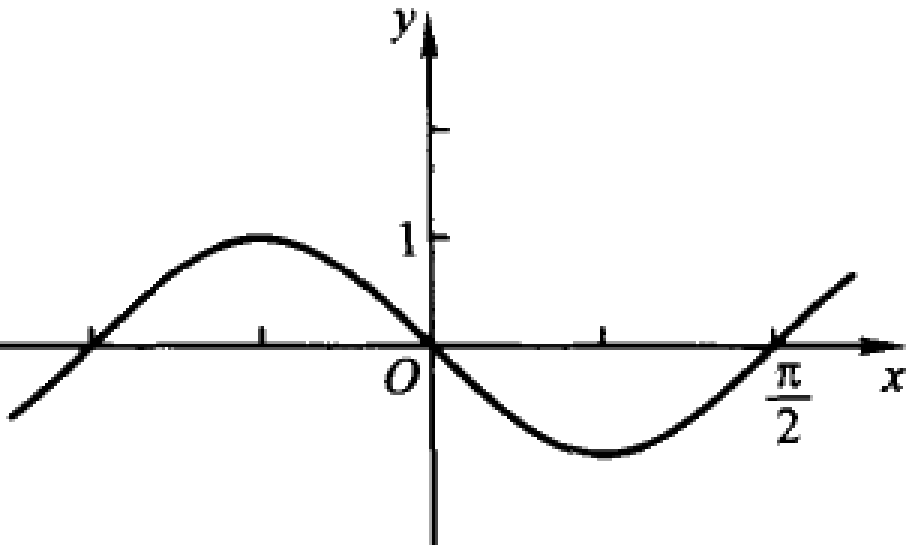
\includegraphics[width=0.48\textwidth]{work/figures/fig2-19}
\figcap\label{fig:2-19}
\end{figure}

\begin{xiti}
\item 对下列函数分别讨论函数的定义域和值域，奇偶性，周期性，有界性，并作出函数的图形：
  \begin{ziti}
  \item $y=|x|$；
  \item $y=x-[x]$；
  \item $y=\tan|x|$；
  \item $y=\sqrt{x(2-x)}$；
  \item $y=\sin^2 x$；
  \item $y=|\sin x|+|\cos x|$．
  \end{ziti}
\item 若已知函数 $y=f(x)$ 的图形，作函数
\[
y_1=|f(x)|,\qquad y_2=f(-x),\qquad y_3=-f(-x)
\]
的图形，并说明 $y_1,y_2,y_3$ 的图形与 $y$ 的图形的关系．
\item 若已知 $f(x),g(x)$ 的图形，试作函数
\[
y=\frac{1}{2}\bigl[f(x)+g(x)\pm\bigl|f(x)-g(x)\bigr|\bigr]
\]
的图形，并说明 $y$ 的图形与 $f(x),g(x)$ 图形的关系．
\item 作出下列函数的图形：
  \begin{ziti}
  \item $y=x\sin x$；
  \item $y=\sin\dfrac{1}{x}$．
  \end{ziti}
\item 符号函数的定义是
\[
y=\sgn x=\begin{cases}
1, & x>0,\\
0, & x=0,\\
-1, & x<0,
\end{cases}
\]
试分别作出 $\sgn x$，$\sgn(2x)$，$\sgn(x-2)$ 的图形．
\item 作出下列函数的图形：
  \begin{ziti}
  \item $y=\sgn\cos x$；
  \item $y=[x]-2\left[\dfrac{x}{2}\right]$．
  \end{ziti}
\end{xiti}

\chapter{极限与函数的连续性}\label{chap:03}

本章讲述数列的极限、具有连续变量的函数的极限以及函数连续的概念．极限的概念与技巧将贯穿全书，本章只是一个引论，以后将逐步深入．因此，在本章中只要求读者对极限在直观了解的基础上，能正确叙述不同变化过程的极限定义，并用于证明极限的四则运算与不等式运算．本章的重要结论之一是，初等函数在它的定义域内都是连续的．

\section{极限问题的提出}\label{sec:3.1}

17 世纪建立的微积分，已有了较为一般的概念，更重要的是提供了一套关于连续变量的崭新的算法，从而成为解决天文、力学、光学与技术问题的重要工具．但那时的微积分，只能说是直观的微积分．因为它的一些基本概念并不确切，甚至逻辑推导前后矛盾．例如，微积分的一个最重要的概念——微商，它反映了一个连续量对另一个连续量的``瞬时变化率''，其概念就很不确切，逻辑推导前后矛盾．牛顿当时把连续量称为流量，把变化率称为流数（把自变量理解为时间）．例如把自由落体的路程看作流量，流数就是瞬时速度．用今天的符号，牛顿当时推导流数的方法是：对自由落体的运动规律 $s = \frac{1}{2}gt^2$，给时间 $t$ 一个微小的改变 $h$（他称之为瞬——moment），则平均速度为
\[
\frac{\frac{1}{2}g(t+h)^2-\frac{1}{2}gt^2}{h} = gt + \frac{1}{2}gh.
\]
然后令 $h=0$，便得瞬时速度 $gt$．凭着类似的推导，微积分的演算系统建立起来了．但这里的瞬 $h$ 究竟是什么？贝克莱（Berkeley，1685---1753）就曾指出这里有逻辑错误．因为在计算平均速度时，要用 $h$ 去除，必须假设 $h \neq 0$．但为最后得到瞬时速度，必须令 $h=0$，才能算出 $gt$．$h$ 非零又是零，$h$ 到底是什么？难怪贝克莱讥讽说这是``消失的量的鬼魂''．这个问题困惑了数学家很长时间．达朗贝尔认为说清楚这点，应该用极限，但他并没有把它说清楚．拉格朗日企图用代数推演的方法逃避这个困难，但这脱离了微积分的物理意义，很难应用．直到 19 世纪柯西才真正用极限的概念把它基本说清楚，而魏尔斯特拉斯最终用 $\varepsilon - \delta$ 的语言，彻底解决了这个困难，从而推动了近代分析的蓬勃发展．

极限最早的观念，在国外有所谓``穷竭法''，在中国有所谓割圆术，即把圆近似地割成边数很多、边长很细的正多边形来计算圆面积．魏晋时代的刘徽就说过：``割之弥细，所失弥小，割之又割，以至于不可割，则与圆周合体而无所失矣''．后来，和微积分同时产生而用得很多的一种运算，就是无穷多项相加
\[
a_1 + a_2 + \cdots + a_n + \cdots.
\]
怎样理解这无穷多项相加？这只能理解为有限项相加，但越加越多，最后看它的变化趋势，这就是所谓的数列极限．把数列极限的思想用来观察求瞬时速度的推导，就是把 $h$ 看成越变越小而且无限地变小（但不为零），来研究平均速度的变化趋势，从而建立一套从平均速度求瞬时速度的计算方法，这就是所谓的函数极限．今天，我们学习微积分，当然不必重复历史的过程，而可以从严格的极限概念开始，严格地讲述微积分的概念、演算及应用．

下面我们先从数列极限入手，然后讲述函数极限，再用函数极限，给出函数连续的概念，并最后证明，一切初等函数在其定义域是连续的．从下一章开始转入微积分．

\section{数列的极限}\label{sec:3.2}

\begin{definition}\label{def:3-1}
定义域为正整数的函数称为数列，记为 $\{x_n\}$．即有 $x_n = f(n)$，$n \in \mathbb{N}_+$．
\end{definition}

$x_n$ 是数列的第 $n$ 项，表示函数在 $n$ 处的函数值，而 $\{x_n\}$ 则表示数列．由于正整数有自然的顺序，故数列也可以写成
\[
x_1, x_2, x_3, \cdots, x_n, \cdots.
\]
这也是数列的一种表示．

$x_n$ 也叫做数列的通项，我们经常可以通过给出第 $n$ 项 $x_n$ 的显式来给出一个数列．

例如 $x_n = \frac{1}{n}$，写出来就是 $1, \frac{1}{2}, \frac{1}{3}, \frac{1}{4}, \cdots$；

$x_n = \frac{(-1)^n}{n}$，写出来就是 $-1, \frac{1}{2}, -\frac{1}{3}, \frac{1}{4}, \cdots$；

$x_n = \frac{n+1}{n}$，写出来就是 $2, \frac{3}{2}, \frac{4}{3}, \frac{5}{4}, \cdots$；

$x_n = n^2$，写出来就是 $1, 4, 9, 16, \cdots$；

$x_n = 1+(-1)^n$，写出来就是 $0, 2, 0, 2, \cdots$．

也有些数列的通项不能用显式表示出来．

例如，$c$ 是无理数，它可用无限不循环小数表示
\[
c_0.c_1c_2\cdots c_n\cdots.
\]
令 $x_n = c_0.c_1c_2\cdots c_n$，这样定义的数列 $\{x_n\}$，一般说来，它的通项不能用显式表示出来．

数列也可以用递推的方法给出，例如，$a_0 = 0$，$a_1 = 1$，$a_{n+1} = \frac{a_{n-1}+a_n}{2}$，$n=1,2,\cdots$ 就定义一个数列，它的前六项是
\[
0, 1, \frac{1}{2}, \frac{3}{4}, \frac{5}{8}, \frac{11}{16}.
\]

\subsection*{1. 极限的概念}

根据§\ref{sec:3.1}问题的提出，我们要研究数列的极限，就是看当 $n$ 无限增大时，$x_n$ 的变化趋势如何．换句话说，看是否存在一个常数 $a$，当 $n$ 无限增大时，$x_n$ 的值无限地接近 $a$．在回答是肯定的情形下，就可以说 $\{x_n\}$ 的极限是 $a$．

我们来看前面提出的几个例子．

\begin{example}\label{ex:3-2-1}
$x_n = \frac{1}{n}$．容易看出，当 $n$ 无限增大时，$x_n$ 无限接近于 $0$，因而 $x_n$ 的极限为 $0$．
\end{example}

\begin{example}\label{ex:3-2-2}
$x_n = \frac{(-1)^n}{n}$．当 $n$ 无限增大时，它的值时而为正，时而为负，但总的趋势仍然是无限地接近于 $0$ 这个数，因此 $x_n$ 的极限也是 $0$．
\end{example}

\begin{example}\label{ex:3-2-3}
$x_n = \frac{n+1}{n}$，即
\[
2, \frac{3}{2}, \frac{4}{3}, \frac{5}{4}, \cdots, \frac{101}{100}, \frac{102}{101}, \cdots,
\]
当 $n$ 无限增大时，$x_n$ 越变越小，无限地接近于 $1$，因此 $x_n$ 的极限是 $1$．
\end{example}

\begin{example}\label{ex:3-2-4}
$x_n = n^2$．当 $n$ 无限增大时，$n^2$ 也无限增大，并不无限接近一个常数，因此说它没有极限．
\end{example}

\begin{example}\label{ex:3-2-5}
$x_n = 1+(-1)^n$．它在 $0$ 与 $2$ 两个数中不停地跳动，也不是无限地接近一个常数，因此也没有极限．
\end{example}

现在我们可以来分析一下，一般地说，当 $n$ 无限增大时，$x_n$ 无限接近于 $a$，确切的意思究竟是什么？

两个数接近的程度可以用它们的差的绝对值（在数轴上，就是这两个点之间的距离）来衡量．因此，以 $x_n = \frac{1}{n}$ 为例，说 $x_n$ 与 $0$ 很接近，即是说 $x_n$ 与 $0$ 的距离 $|x_n - 0|$ 很小．例如
\[
\text{当 } n>2 \text{ 时},\quad |x_n - 0| = \frac{1}{n} < \frac{1}{2},
\]
当 $n>3$ 时，$|x_n - 0| = \frac{1}{n} < \frac{1}{3}$，

当 $n>N$ 时，$|x_n - 0| = \frac{1}{n} < \frac{1}{N}$．

上面左边一列是 $n$ 增大的程度．相应地，右边一列是 $x_n$ 与 $0$ 的接近程度．$n$ 增大的程度不同，则 $x_n$ 与 $0$ 的接近程度也不同．$n$ 只要大到比 $N$ 大，就可以保证 $x_n$ 与 $0$ 的距离小于 $\frac{1}{N}$．直观形象地说，如果把数列
\[
x_1, x_2, \cdots, x_N, x_{N+1}, x_{N+2}, \cdots
\]
从第 $N+1$ 项起后面的所有项叫做数列 $\{x_n\}$ 的尾巴，则尾巴中的每项与 $0$ 的距离都小于 $\frac{1}{N}$．

我们已经看到，对于足够大的 $N$ 之后的所有 $n$，可以使 $|x_n - 0|$ 小到一定程度，但还不能说明 $|x_n - 0|$ 无限小．如何反映``无限''二字呢？我们说当 $n$ 无限增大时，$x_n$ 无限接近于 $0$，即是说 $x_n$ 与 $0$ 的距离 $|x_n - 0|$ 可以任意小，只要 $n$ 足够大（$n > N$）．可见``无限''能用距离的任意性来反映，即对于任意的正数 $\varepsilon$，不论它多么小，只要 $N$ 足够大，对于所有的 $n > N$，都能保证 $|x_n - 0| < \varepsilon$．事实上，要使
\[
|x_n - 0| = \frac{1}{n} < \varepsilon,
\]
只要 $n > \frac{1}{\varepsilon}$．故取 $N = \left[\frac{1}{\varepsilon}\right]$，则对大于 $N$ 的所有正整数 $n$，上式总成立．

将上面的语言抽象化，便有下面的定义．

\begin{definition}\label{def:3-2}
设 $\{x_n\}$ 是一数列，$a$ 是一实数．若对于任意给定的正数 $\varepsilon$，存在正整数 $N$，当 $n > N$ 时，都有
\[
|x_n - a| < \varepsilon,
\]
则称 $a$ 是数列 $\{x_n\}$ 当 $n$ 趋于无穷时的极限，或称数列 $\{x_n\}$ 收敛，且收敛于 $a$，记为
\[
\lim_{n\to\infty}x_n = a,\qquad \text{或}\qquad x_n \to a\quad(n\to\infty).
\]
没有极限的数列称为发散数列．
\end{definition}

从几何上看，数列 $\{x_n\}$ 的极限为 $a$，是指任意给定以 $a$ 为中心的区间 $(a-\varepsilon, a+\varepsilon)$，必然从某项 $x_{N+1}$ 起，后面的所有项都落在区间 $(a-\varepsilon, a+\varepsilon)$ 之中．换句话说，数列 $\{x_n\}$ 至多有 $N$ 项 $x_1, x_2, \cdots, x_N$ 落在区间 $(a-\varepsilon, a+\varepsilon)$ 之外（见图~\ref{fig:3-1}）．这就是数列极限的几何意义．由此也可以看出，数列的前有限项并不影响数列的收敛性和极限．即添加或修改数列的有限项，并不影响数列的收敛性与极限．

\begin{figure}[htbp]
\centering
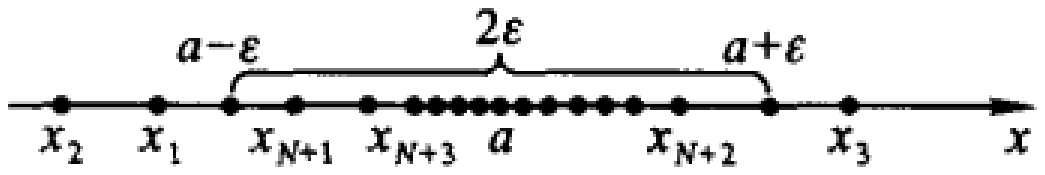
\includegraphics[width=0.72\textwidth]{work/figures/fig3-1}
\figcap\label{fig:3-1}
\end{figure}

定义中描述数列极限的语言称为 $\varepsilon - N$ 语言．正数 $\varepsilon$ 用来反映 $x_n$ 与 $a$ 的接近程度，而 $\varepsilon$ 的任意性就反映了 $x_n$ 与 $a$ 可以任意接近，或说无限接近．$\varepsilon$ 是任意的，也是相对固定的．对每一个固定的 $\varepsilon > 0$，相应地有一个 $N$，$N$ 是随 $\varepsilon$ 的变化而变化的．一般地说，$\varepsilon$ 越小则 $N$ 越大．$N$ 一旦存在则不是唯一的，不过重要的是 $N$ 的存在性，而不是 $N$ 取什么值．

\begin{definition}\label{def:3-3}
极限为 $0$ 的数列称为无穷小量．
\end{definition}

值得注意的是无穷小量是一数列，而不是一个很小的常数．由极限定义显然有，$\{x_n\}$ 以 $a$ 为极限等价于数列 $\{x_n - a\}$ 以 $0$ 为极限．我们把它写成下面的命题．

\begin{proposition}\label{prop:3-1}
$\{x_n\}$ 的极限为 $a$ 的充要条件是 $\{x_n - a\}$ 是无穷小量．
\end{proposition}

数列极限定义本身并没有给出求极限的方法，但它却深刻地描述了数列趋向极限的变化过程．当估计出数列的极限后，可以用定义来验证估计的正确性．下面举例说明．

\begin{example}\label{ex:3-2-6}
证明 $\lim_{n\to\infty}\frac{1}{n^p} = 0$ ($p>0$)．
\end{example}

\begin{proof}
对任意给定的 $\varepsilon>0$，要使
\[
\left|\frac{1}{n^p} - 0\right| = \frac{1}{n^p} < \varepsilon,
\]
只要 $n > \left(\frac{1}{\varepsilon}\right)^{\frac{1}{p}}$．取 $N = \left[\left(\frac{1}{\varepsilon}\right)^{\frac{1}{p}}\right] + 1$，则当 $n > N$ 时，有
\[
\left|\frac{1}{n^p} - 0\right| < \varepsilon.
\]
故 $\left\{\frac{1}{n^p}\right\}$ 的极限为 $0$．
\end{proof}

\begin{example}\label{ex:3-2-7}
设 $|q|<1$，证明 $\lim_{n\to\infty}q^n = 0$．
\end{example}

\begin{proof}[证法 1]
若 $q = 0$，结论显然成立．故不妨设 $q \neq 0$．对任意给定的 $\varepsilon > 0$，不妨设 $\varepsilon < 1$，要使
\[
|q^n - 0| = |q^n| < \varepsilon,
\]
即
\[
n\lg|q| < \lg\varepsilon,
\]
只要
\[
n > \frac{\lg\varepsilon}{\lg|q|}.
\]
令 $N = \left[\frac{\lg\varepsilon}{\lg|q|}\right] + 1$，则当 $n > N$ 时，有 $|q^n| < \varepsilon$．这就证明了 $\lim_{n \to \infty} q^n = 0$．
\end{proof}

\begin{proof}[证法 2]
不妨设 $q \neq 0$．由 $|q| < 1$ 知存在 $\alpha > 0$，使得 $|q| = \frac{1}{1 + \alpha}$，从而
\[
|q|^n = \frac{1}{(1 + \alpha)^n} = \frac{1}{1 + n\alpha + \cdots + \alpha^n} < \frac{1}{n\alpha}.
\]
对任给的 $\varepsilon > 0$，要使 $|q^n| < \varepsilon$，只要放大后的 $\frac{1}{n\alpha} < \varepsilon$．因此取 $N = \left[\frac{1}{\alpha\varepsilon}\right] + 1$，则当 $n > N$ 时，有
\[
|q^n - 0| = |q|^n < \frac{1}{n\alpha} < \varepsilon.
\]
这就证明了 $\lim_{n\to\infty}q^n = 0$．
\end{proof}

从前面的例子可见，整个证明过程实际上是找 $N$ 的过程，采用的是反推法，即从 $|x_n - a| < \varepsilon$ 出发，看满足条件的 $N$ 是否存在．我们只要找到一个就可以了，不管用的是什么方法．证法 2 用的是适当放大法，它将 $|q^n - 0|$ 适当放大到 $\frac{1}{n\alpha}$，使我们很容易找到 $N$．当然放大要适当，要保证把 $|x_n - a|$ 放大以后仍然是无穷小量．下面再举几个适当放大的例子．

\begin{example}\label{ex:3-2-8}
设 $a > 0$，证明 $\lim_{n \to \infty} \sqrt[n]{a} = 1$．
\end{example}

\begin{proof}
若 $a=1$，结论显然成立．

设 $a > 1$．记 $\sqrt[n]{a} = 1 + \alpha_n$ ($\alpha_n > 0$)，则
\[
a = (1 + \alpha_n)^n = 1 + n\alpha_n + \cdots + \alpha_n^n > n\alpha_n.
\]
因此
\[
|\sqrt[n]{a} - 1| = \alpha_n < \frac{a}{n}.
\]
对任意给定的 $\varepsilon>0$，不妨设 $\varepsilon<1$，取 $N = \left[\frac{a}{\varepsilon}\right]$，则当 $n>N$ 时，有
\[
|\sqrt[n]{a} - 1| < \frac{a}{n} < \varepsilon.
\]
最后设 $0 < a < 1$．这时存在 $b > 1$ 使 $a = \frac{1}{b}$，因此
\[
|\sqrt[n]{a} - 1| = \left|\sqrt[n]{\frac{1}{b}} - 1\right| = \frac{|1 - \sqrt[n]{b}|}{\sqrt[n]{b}} < |1 - \sqrt[n]{b}|.
\]
由于 $\lim_{n\to\infty}\sqrt[n]{b} = 1$，故对任给 $\varepsilon>0$，存在 $N$，当 $n>N$ 时，有
\[
|\sqrt[n]{a} - 1| < |1 - \sqrt[n]{b}| < \varepsilon.
\]
这样，我们证明了当 $a > 0$ 时，总有 $\lim_{n \to \infty} \sqrt[n]{a} = 1$．
\end{proof}

\begin{example}\label{ex:3-2-9}
证明 $\lim_{n\to\infty}\frac{n^2+1}{n^2-n-2} = 1$．
\end{example}

\begin{proof}
当 $n>4$ 时，
\[
\left|\frac{n^2+1}{n^2-n-2} - 1\right| = \left|\frac{n+3}{n^2-n-2}\right| = \frac{n+3}{n^2-n-2} < \frac{2n}{n^2 - \frac{n^2}{4} - \frac{n^2}{4}} = \frac{4}{n}.
\]
对任给的 $\varepsilon>0$，取 $N = \max\left(4, \left[\frac{4}{\varepsilon}\right]\right)$，则当 $n>N$ 时，有
\[
\left|\frac{n^2+1}{n^2-n-2} - 1\right| < \frac{4}{n} < \varepsilon,
\]
即
\[
\lim_{n\to\infty}\frac{n^2+1}{n^2-n-2} = 1.
\]
\end{proof}

研究数列的极限，就是要从数列出发，把它的极限求出来．可见从数列到极限，也是一种运算，但它同第一章讲数系时的运算很不同．那时是从两个数（或有穷个数）出发求一个数，例如从 $a$ 和 $b$ 求 $a+b$．求极限则完全不同了，是从一个数列，即从无穷个数出发，求一个数．从无穷个数到一个数，这就是极限运算的特点．正是由于这个特点，使极限的计算变得十分复杂．因此，人们需要有一个一般的准则来检验计算是否正确．当然，这个准则不仅在检验一些具体数列的极限时是重要的，而更重要的是它对理论上的推理是必不可少的．这个准则就是极限的 $\varepsilon-N$ 定义，它是人类经过漫长的时间才抽象出来的．我们并不要求读者立刻全面地理解，只希望读者在今后的学习过程中，通过大量的反复的应用逐步地掌握它．

\subsection*{2. 极限与四则运算及与不等式的关系}

下面我们要来寻找求极限的方法．

回忆学算术的过程，我们可以计算任何两个数的乘法．为什么呢？实际上，我们所掌握的，一是九九表，二是一套进位规则（当然还包括小数点的计算）．何谓进位规则？其实说的是加法与乘法的分配律，也就是加法与乘法的运算次序可以交换：
\[
a(b+c) = ab + ac.
\]
例如，$26 \times 8 = 208$，是这样计算出来的：
\[
\begin{array}{r}
2\ 6 \\
\times \quad 8 \\
\hline
4\ 8 \\
1\ 6\ 0 \\
\hline
2\ 0\ 8
\end{array}
\]
实际上根据的就是加法与乘法可以交换次序：
\[
26\times8 = (20+6)\times8 = 20\times8 + 6\times8 = 160 + 48 = 208.
\]
因此，我们希望能学会求更多数列的极限，自然就会问，对极限这一新的运算，它和别的运算间是否也有类似的规律？事实上，并非所有的运算都具有类似的性质．例如等式
\[
\sqrt{a+b} = \sqrt{a} + \sqrt{b}
\]
就不是永远成立的，即开平方运算与加法运算并不能交换次序．若能设想这等式成立，开平方运算就会变得简单得多了．

极限是对无穷个数进行的运算，它和四则运算的次序能否交换？幸好，回答是肯定的．当然，这是需要证明的，因为极限运算是一种崭新的运算．

\begin{theorem}\label{thm:3-1}
设 $\lim_{n\to\infty}x_n = a$，$\lim_{n\to\infty}y_n = b$，则
\begin{enumerate}[label=\roman*)]
\item $\lim_{n\to\infty}(x_n \pm y_n) = a \pm b$；
\item $\lim_{n \to \infty} (x_n y_n) = ab$；
\item $\lim_{n \to \infty} \frac{x_n}{y_n} = \frac{a}{b} \quad (b \neq 0)$．
\end{enumerate}
\end{theorem}

定理~\ref{thm:3-1} 表明两数列对应项的代数和（积、商）的极限等于极限的代数和（积、商），因此实际上说的是极限运算和四则运算次序是可以交换的．我们可以把定理~\ref{thm:3-1} 写成
\[
\lim_{n\to\infty}(x_n \pm y_n) = \lim_{n\to\infty}x_n \pm \lim_{n\to\infty}y_n;
\]
\[
\lim_{n\to\infty}(x_n y_n) = \lim_{n\to\infty}x_n \cdot \lim_{n\to\infty}y_n;
\]
\[
\lim_{n\to\infty}\frac{x_n}{y_n} = \frac{\lim\limits_{n\to\infty}x_n}{\lim\limits_{n\to\infty}y_n}\qquad \left(\text{当 }\lim_{n\to\infty}y_n \neq 0\right).
\]
值得注意的是，其前提是等式右边的极限都事先假设是存在的．

为了证明 ii)，我们将要用到收敛数列的有界性．为了证明 iii)，又要用到极限的保号性．因此，我们先给出这两个性质，再回头来证明定理~\ref{thm:3-1}．

回忆函数的有界性定义，知数列 $\{x_n\}$ 有界是指存在正数 $M$，使得
\[
|x_n| \leqslant M
\]
对一切 $n$ 成立．

\begin{theorem}[有界性]\label{thm:3-2}
有极限存在的数列必有界．
\end{theorem}

\begin{proof}
设数列 $\{x_n\}$ 有极限 $a$．由极限定义，对 $\varepsilon_0 = 1$，则存在 $N$，当 $n>N$ 时，有
\[
|x_n - a| < 1.
\]
因此
\[
|x_n| = |x_n - a + a| \leqslant |x_n - a| + |a| < 1 + |a|.
\]
令 $M = \max(|x_1|, |x_2|, \cdots, |x_N|, 1+|a|)$，则
\[
|x_n| \leqslant M,\qquad n=1,2,\cdots.
\]
这就证明了 $\{x_n\}$ 是有界的．
\end{proof}

\begin{corollary}\label{cor:3-1}
若 $\{x_n\}$ 无界，则 $\{x_n\}$ 发散．
\end{corollary}

\begin{theorem}[保号性]\label{thm:3-3}
若 $\lim_{n\to\infty}x_n = a$，$a>0$，则存在 $N$，当 $n>N$ 时，有 $x_n > \frac{a}{2} > 0$．
\end{theorem}

\begin{proof}
由 $\lim_{n\to\infty}x_n = a > 0$，知对 $\varepsilon_0 = \frac{a}{2} > 0$，存在 $N$，当 $n>N$ 时，有
\[
|x_n - a| < \frac{a}{2},
\]
从而
\[
x_n > a - \frac{a}{2} = \frac{a}{2} > 0.
\]
定理证完（见图~\ref{fig:3-2}）．
\end{proof}

\begin{figure}[htbp]
\centering
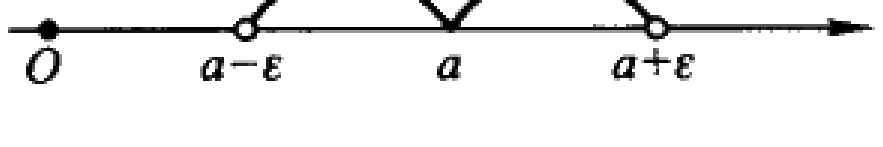
\includegraphics[width=0.48\textwidth]{work/figures/fig3-2}
\figcap\label{fig:3-2}
\end{figure}

\begin{corollary}\label{cor:3-2}
设 $\lim_{n\to\infty}x_n = a$．
\begin{enumerate}[label=\roman*)]
\item 若 $a<0$，则存在 $N$，当 $n>N$ 时，有 $x_n < \frac{a}{2} < 0$；
\item 若 $a \neq 0$，则存在 $N$，当 $n > N$ 时，有 $|x_n| > \frac{|a|}{2} > 0$．
\end{enumerate}
\end{corollary}

请读者写出推论~\ref{cor:3-2} 的证明．

\begin{proof}[定理~\ref{thm:3-1} 的证明]
i) 对任意给定的 $\varepsilon>0$，由 $\lim_{n\to\infty} x_n = a$，存在 $N_1$，当 $n>N_1$ 时，有
\[
|x_n - a| < \frac{\varepsilon}{2}.
\]
由 $\lim_{n\to\infty}y_n = b$，知存在 $N_2$，当 $n>N_2$ 时，有
\[
|y_n - b| < \frac{\varepsilon}{2}.
\]
取 $N = \max(N_1, N_2)$，则当 $n > N$ 时，有
\[
|x_n \pm y_n - (a \pm b)| \leqslant |x_n - a| + |y_n - b| < \frac{\varepsilon}{2} + \frac{\varepsilon}{2} = \varepsilon,
\]
即
\[
\lim_{n\to\infty}(x_n \pm y_n) = a \pm b.
\]

ii) 对任意 $n$，有
\[
\begin{aligned}
|x_n y_n - ab| &= |x_n y_n - x_n b + x_n b - ab| \\
&\leqslant |x_n y_n - x_n b| + |x_n b - ab| \\
&= |x_n||y_n - b| + |b||x_n - a|.
\end{aligned}
\]
任给 $\varepsilon>0$，由 $\lim_{n\to\infty}x_n = a$ 与 $\lim_{n\to\infty}y_n = b$，以及定理~\ref{thm:3-2}，知存在 $M>0$，使
\[
|x_n| \leqslant M,\qquad n=1,2,\cdots,
\]
同时存在 $N_1$，当 $n > N_1$ 时，有
\[
|x_n - a| < \frac{\varepsilon}{2(|b|+1)},
\]
并存在 $N_2$，当 $n > N_2$ 时，有
\[
|y_n - b| < \frac{\varepsilon}{2M}.
\]
令 $N = \max(N_1, N_2)$，则当 $n > N$ 时，有
\[
|x_n y_n - ab| \leqslant |x_n||y_n - b| + |b||x_n - a| < M\frac{\varepsilon}{2M} + |b|\frac{\varepsilon}{2(|b|+1)} < \varepsilon.
\]
这就证明了 $\lim_{n\to\infty}x_n y_n = ab$．

iii) 由 $\lim_{n\to\infty}y_n = b \neq 0$，根据推论~\ref{cor:3-2}，存在 $N_1$，当 $n>N_1$ 时，有
\[
|y_n| > \frac{|b|}{2} > 0,
\]
从而当 $n>N_1$ 时有
\[
\left|\frac{x_n}{y_n} - \frac{a}{b}\right| = \frac{|b x_n - a y_n|}{|y_n||b|} \leqslant \frac{|b||x_n - a| + |a||y_n - b|}{\frac{1}{2}|b|^2}.
\]
已知 $\lim_{n\to\infty}x_n = a$ 和 $\lim_{n\to\infty}y_n = b$，由极限定义，对任意给定的 $\varepsilon>0$，存在 $N_2$，当 $n>N_2$ 时，有
\[
|x_n - a| < \frac{|b|}{4}\varepsilon,
\]
存在 $N_3$，当 $n > N_3$ 时，有
\[
|y_n - b| < \frac{|b|^2}{4(|a|+1)}\varepsilon.
\]
令 $N = \max(N_1, N_2, N_3)$，则当 $n > N$ 时，有
\[
\left|\frac{x_n}{y_n} - \frac{a}{b}\right| \leqslant \frac{2}{|b|}|x_n - a| + \frac{2|a|}{|b|^2}|y_n - b| < \frac{\varepsilon}{2} + \frac{\varepsilon}{2} = \varepsilon.
\]
这就证明了 $\lim_{n\to\infty}\frac{x_n}{y_n} = \frac{a}{b}$．
\end{proof}

当 $x_n = c$ 时，我们由 ii) 得到下面的推论．

\begin{corollary}\label{cor:3-3}
若 $\lim_{n\to\infty}y_n = b$，$c$ 是常数，则
\[
\lim_{n\to\infty}(c y_n) = cb.
\]
\end{corollary}

在定理~\ref{thm:3-2} 和定理~\ref{thm:3-3} 的证明中，$\varepsilon$ 不是任意的，而是取定了某 $\varepsilon_0$，$\varepsilon_0$ 不变才能保证 $N$ 固定不变．而在定理~\ref{thm:3-1} 的证明中 $\varepsilon$ 都是任意的．请注意区别什么时候可以取定 $\varepsilon$，而什么时候 $\varepsilon$ 必须是任意的．

由定理~\ref{thm:3-1} 的 i) 以及 ii) 立即可知，无穷小量的代数和、积仍是无穷小量．对于积，我们还有下面的结论，它对求极限是很方便的．

\begin{theorem}\label{thm:3-4}
若 $\{x_n\}$ 是无穷小量，$\{y_n\}$ 是有界数列，则 $\{x_n y_n\}$ 是无穷小量．
\end{theorem}

\begin{proof}
对任意给定的 $\varepsilon>0$，首先由 $\{y_n\}$ 是有界数列，知存在 $M>0$，使得
\[
|y_n| \leqslant M,\qquad n=1,2,\cdots.
\]
其次由 $\{x_n\}$ 是无穷小量，知存在 $N$，当 $n > N$ 时，有
\[
|x_n| < \frac{\varepsilon}{M}.
\]
因此，当 $n > N$ 时，有
\[
|x_n y_n| \leqslant M|x_n| < \varepsilon.
\]
定理证完．
\end{proof}

\begin{example}\label{ex:3-2-10}
求 $\lim_{n\to\infty}\frac{1}{n}\sin n$．
\end{example}

\begin{proof}[解]
因为 $\lim_{n\to\infty}\frac{1}{n} = 0$，而 $\{\sin n\}$ 是有界数列，所以
\[
\lim_{n\to\infty}\frac{1}{n}\sin n = 0.
\]
\end{proof}

\begin{example}\label{ex:3-2-11}
求 $\lim_{n\to\infty}\frac{4n^2+1}{2n^2+5n-6}$．
\end{example}

\begin{proof}[解]
\[
\lim_{n\to\infty}\frac{4n^2+1}{2n^2+5n-6} = \lim_{n\to\infty}\frac{4+\frac{1}{n^2}}{2+\frac{5}{n}-\frac{6}{n^2}} = \frac{4+\lim\limits_{n\to\infty}\frac{1}{n^2}}{2+\lim\limits_{n\to\infty}\frac{5}{n}-\lim\limits_{n\to\infty}\frac{6}{n^2}} = 2.
\]
\end{proof}

更一般地，若 $a_0 \neq 0$，$b_0 \neq 0$，$k,l$ 是正整数，$k \leqslant l$，则
\[
\lim_{n\to\infty}\frac{a_0 n^k + a_1 n^{k-1} + \cdots + a_k}{b_0 n^l + b_1 n^{l-1} + \cdots + b_l} = \lim_{n\to\infty}n^{k-l}\frac{a_0 + \frac{a_1}{n} + \cdots + \frac{a_k}{n^k}}{b_0 + \frac{b_1}{n} + \cdots + \frac{b_l}{n^l}} = \begin{cases}
\frac{a_0}{b_0}, & k = l,\\
0, & k < l.
\end{cases}
\]

下面研究极限运算与不等式的关系．

\begin{theorem}[保序性]\label{thm:3-5}
若 $\lim_{n\to\infty}x_n = a$，$\lim_{n\to\infty}y_n = b$，且 $a>b$，则存在 $N$，当 $n>N$ 时，有 $x_n > y_n$．
\end{theorem}

\begin{proof}[证法 1]
（用定理~\ref{thm:3-3} 的证明方法）对 $\varepsilon_0 = \frac{a-b}{2}$，由 $\lim_{n\to\infty}x_n = a$，知存在 $N_1$，当 $n>N_1$ 时，有
\[
|x_n - a| < \frac{a-b}{2},
\]
则有
\[
\frac{a+b}{2} < x_n.
\]
又由 $\lim_{n\to\infty}y_n = b$，知存在 $N_2$，当 $n>N_2$ 时，有
\[
|y_n - b| < \frac{a-b}{2},
\]
则有
\[
y_n < \frac{a+b}{2}.
\]
令 $N = \max(N_1, N_2)$，则当 $n > N$ 时，有
\[
y_n < \frac{a+b}{2} < x_n.
\]
定理证完（见图~\ref{fig:3-3}）．
\end{proof}

\begin{figure}[htbp]
\centering
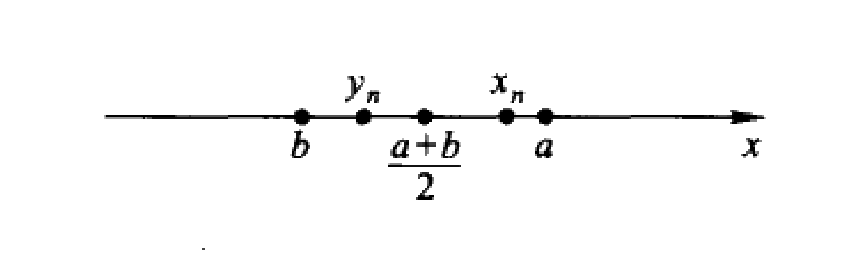
\includegraphics[width=0.55\textwidth]{work/figures/fig3-3}
\figcap\label{fig:3-3}
\end{figure}

\begin{proof}[证法 2]
令 $z_n = x_n - y_n$，则
\[
\lim_{n\to\infty}z_n = \lim_{n\to\infty}(x_n - y_n) = a - b > 0.
\]
由定理~\ref{thm:3-3}，存在 $N$，当 $n > N$ 时，有
\[
z_n = x_n - y_n > \frac{a-b}{2} > 0,
\]
即 $x_n > y_n$．这又证明了定理~\ref{thm:3-5}．
\end{proof}

值得指出的是，证法 1 用的是定理~\ref{thm:3-3} 的证明方法，证法 2 用的是定理~\ref{thm:3-3} 的结论．用定理的结论，和用定理的证明方法，是不同的两回事．对一个定理，既要学会用它的结论，也要学会用它的证明方法，这是以后学习要注意的．

\begin{theorem}[极限不等式]\label{thm:3-6}
若对任意正整数 $n$ 有 $x_n \leqslant y_n$，且 $\lim_{n \to \infty} x_n = a$，$\lim_{n \to \infty} y_n = b$，则 $a \leqslant b$．
\end{theorem}

\begin{proof}
用反证法．如果不然，设 $a > b$，则由定理~\ref{thm:3-5}，存在 $N$，当 $n > N$ 时有 $x_n > y_n$，与假设条件矛盾．故必有 $a \leqslant b$．
\end{proof}

注意到数列的前有限项并不影响数列的极限，因此定理~\ref{thm:3-6} 的条件可以减弱为``存在 $N$，当 $n > N$ 时有 $x_n \leqslant y_n$''．

如果将条件``$x_n \leqslant y_n$''改为``$x_n < y_n$''，并不能得到 $a < b$ 的结论．例如 $\frac{n-1}{n} < \frac{n+1}{n}$，但
\[
\lim_{n\to\infty}\frac{n-1}{n} = \lim_{n\to\infty}\frac{n+1}{n} = 1.
\]
可见结论也只能得到 $a \leqslant b$．定理~\ref{thm:3-6} 表明，在极限存在的前提下，可以在不等式两边取极限，但千万不要忘记``带上等号''．

用上面的方法，我们实际上已证明了极限的唯一性，即一个数列不可能有两个不同的极限值．

\begin{theorem}[唯一性]\label{thm:3-7}
若数列有极限存在，则极限是唯一的．
\end{theorem}

\begin{proof}
用反证法．如果不然，设 $\{x_n\}$ 有极限 $a$ 和 $b$，$a \neq b$，不妨设 $a < b$．对 $\varepsilon = \frac{b - a}{2} > 0$，存在 $N_1$，当 $n > N_1$ 时，有
\[
x_n < a + \varepsilon = \frac{a+b}{2},
\]
同样存在 $N_2$，当 $n > N_2$ 时，有
\[
x_n > b - \varepsilon = \frac{a+b}{2},
\]
故当 $n > \max (N_1, N_2)$ 时，有
\[
x_n < a + \varepsilon = b - \varepsilon = \frac{a+b}{2} < x_n,
\]
这是不可能的，这就证明了极限的唯一性．
\end{proof}

\begin{theorem}[夹迫性]\label{thm:3-8}
如果对任意正整数 $n$，有
\[
x_n \leqslant y_n \leqslant z_n,
\]
且 $\lim_{n\to\infty}x_n = \lim_{n\to\infty}z_n = a$，则 $\lim_{n\to\infty}y_n$ 存在且等于 $a$．
\end{theorem}

\begin{proof}
对任意给定的 $\varepsilon > 0$，由 $\lim_{n \to \infty} x_n = \lim_{n \to \infty} z_n = a$，存在 $N_1$，当 $n > N_1$ 时，有
\[
|x_n - a| < \varepsilon,\qquad \text{即}\quad a-\varepsilon < x_n < a+\varepsilon.
\]
存在 $N_2$，当 $n > N_2$ 时，有
\[
|z_n - a| < \varepsilon,\qquad \text{即}\quad a-\varepsilon < z_n < a+\varepsilon.
\]
令 $N = \max(N_1, N_2)$，则当 $n > N$ 时，有
\[
a-\varepsilon < x_n \leqslant y_n \leqslant z_n < a+\varepsilon,
\]
即
\[
|y_n - a| < \varepsilon.
\]
故 $\lim_{n\to\infty}y_n$ 存在且等于 $a$，定理证完．
\end{proof}

\begin{example}\label{ex:3-2-12}
设 $x_n = \sqrt[n]{A^n + B^n}$，其中 $A>B>0$，求证 $\lim_{n\to\infty}x_n = A$．
\end{example}

\begin{proof}
由于
\[
A = \sqrt[n]{A^n} \leqslant \sqrt[n]{A^n + B^n} \leqslant \sqrt[n]{2A^n} = \sqrt[n]{2}A,
\]
而
\[
\lim_{n\to\infty}\sqrt[n]{2}A = 1\cdot A = A,
\]
由定理~\ref{thm:3-8} 即得 $\lim_{n\to\infty}\sqrt[n]{A^n + B^n} = A$．
\end{proof}

\begin{example}\label{ex:3-2-13}
证明 $\lim_{n\to\infty}\sqrt[n]{n} = 1$．
\end{example}

\begin{proof}[证法 1]
当 $n > 1$ 时，$\sqrt[n]{n} > 1$，令 $\sqrt[n]{n} = 1 + h_n$，其中 $h_n > 0$．这时
\[
n = (1+h_n)^n = 1 + nh_n + \frac{n(n-1)}{2}h_n^2 + \cdots + h_n^n \geqslant \frac{n(n-1)}{2}h_n^2,
\]
因此 $h_n \leqslant \sqrt{\frac{2}{n-1}}$．故
\[
1 < \sqrt[n]{n} = 1 + h_n \leqslant 1 + \sqrt{\frac{2}{n-1}}.
\]
已知
\[
\lim_{n\to\infty}\left(1 + \sqrt{\frac{2}{n-1}}\right) = 1 + \lim_{n\to\infty}\sqrt{\frac{2}{n-1}} = 1,
\]
由定理~\ref{thm:3-8} 得 $\lim_{n\to\infty}\sqrt[n]{n} = 1$．
\end{proof}

\begin{proof}[证法 2]
当 $n>1$ 时，由平均值不等式得
\[
1 < \sqrt[n]{n} = \sqrt[n]{\sqrt{n}\cdot\sqrt{n}\cdot1\cdots1} \leqslant \frac{\sqrt{n} + \sqrt{n} + n - 2}{n} = \frac{2}{\sqrt{n}} + 1 - \frac{2}{n}.
\]
而
\[
\lim_{n\to\infty}\left(\frac{2}{\sqrt{n}} + 1 - \frac{2}{n}\right) = 1,
\]
由定理~\ref{thm:3-8} 得 $\lim_{n\to\infty}\sqrt[n]{n} = 1$．
\end{proof}

回忆函数单调性定义，我们说数列 $\{x_n\}$ 单调上升（下降），是指 $x_n \leqslant x_{n+1}$（$x_n \geqslant x_{n+1}$）对一切 $n$ 成立．

\begin{theorem}\label{thm:3-9}
单调上升（下降）有上（下）界的数列必有极限存在．
\end{theorem}

\begin{proof}
设数列 $\{x_n\}$ 单调上升有上界．令 $B$ 是 $\{x_n\}$ 全体上界组成的集合，即
\[
B = \{b\mid x_n \leqslant b,\,\forall n\},
\]
而
\[
A = \mathbb{R}\setminus B,
\]
则 $A \mid B$ 是实数的一个分划．事实上，由 $\{x_n\}$ 有上界，知 $B$ 不空．又 $\{x_n\}$ 单调上升，故 $x_1 - 1 \in A$，即 $A$ 不空．由 $A = \mathbb{R} \setminus B$ 知，$A,B$ 不漏．又对任给 $a \in A, b \in B$，则存在 $n_0$，使 $a < x_{n_0} \leqslant b$，即 $A,B$ 不乱．故 $A \mid B$ 是实数的一个分划．根据实数基本定理，存在 $\alpha \in \mathbb{R}$ 使得对任意 $a \in A$，任意 $b \in B$，有 $a \leqslant \alpha \leqslant b$．

下证 $\lim_{n\to\infty}x_n = \alpha$．事实上，对任给 $\varepsilon>0$，由于 $\alpha-\varepsilon \in A$，知存在 $N$，使 $\alpha-\varepsilon < x_N$，又 $\{x_n\}$ 单调上升，故当 $n>N$ 时，有 $\alpha-\varepsilon < x_N \leqslant x_n$．注意到 $\alpha+\frac{\varepsilon}{2} \in B$，便有 $x_n \leqslant \alpha+\frac{\varepsilon}{2}$，故当 $n>N$ 时有
\[
\alpha-\varepsilon < x_n \leqslant \alpha+\frac{\varepsilon}{2},
\]
于是
\[
|x_n - \alpha| < \varepsilon.
\]
这就证明了 $\lim_{n\to\infty}x_n = \alpha$．

显然，单调下降的情形同样可以用上述证明方法给出，但也可以用上述结论证明．事实上，若 $\{x_n\}$ 单调下降有下界，令 $y_n = -x_n$，则 $\{y_n\}$ 就单调上升有上界，从而有极限．设极限为 $\alpha$，则
\[
\lim_{n\to\infty}x_n = \lim_{n\to\infty}(-y_n) = -\lim_{n\to\infty}y_n = -\alpha.
\]
定理证完．
\end{proof}

定理~\ref{thm:3-9} 是只断言极限存在，而没有给出如何计算极限的第一个定理．但即使只给出极限存在，有时已能提供计算的方法．

\begin{example}\label{ex:3-2-14}
设
\[
\begin{aligned}
&x_1 = \sqrt{2},\quad x_2 = \sqrt{2+\sqrt{2}},\\
&x_{n+1} = \sqrt{2+x_n} = \sqrt{2+\sqrt{2+\cdots+\sqrt{2}}},\qquad n=2,3,\cdots,
\end{aligned}
\]
求 $\{x_n\}$ 的极限．
\end{example}

\begin{proof}[解]
显然 $\{x_n\}$ 是单调上升的，下面用数学归纳法证明 $\{x_n\}$ 有上界．显然 $x_1 = \sqrt{2} < 2$．若 $x_n \leqslant 2$，则
\[
x_{n+1} = \sqrt{2+x_n} \leqslant \sqrt{2+2} = 2.
\]
故 $\{x_n\}$ 单调上升有上界，从而必有极限．设极限为 $a$，由
\[
x_{n+1}^2 = 2 + x_n,
\]
令 $n \to \infty$，即得 $a^2 = 2 + a$．解得 $a = -1$ 或 $a = 2$．由于 $x_n \geqslant \sqrt{2}$，故必有 $a \geqslant \sqrt{2}$．舍去 $a = -1$，得 $a = 2$，即 $\lim_{n \to \infty} x_n = 2$．
\end{proof}

通常我们称定理~\ref{thm:3-9} 为单调有界原理，它的意义在于给出了数列极限存在的一个判别方法．与极限定义相比，它并不需要预先估计极限值，相反，如上例表明的，有时在用它证明了极限存在的情况下，通过极限的运算可以方便地求出极限值．但务必注意，在这里极限存在性的前提是非常重要的．考察数列 $x_n = (-1)^n$，显然 $\{x_n\}$ 的极限不存在（本节习题 10），但它满足 $x_{n+1} = -x_n$．令 $n\to\infty$ 两边取极限，便得 $a = -a$，即 $a = 0$．这显然是荒谬的结果．

最后，我们用单调有界原理证明一个重要数列极限的存在性．

\begin{example}\label{ex:3-2-15}
证明数列 $\left\{\left(1+\frac{1}{n}\right)^n\right\}$ 的极限存在．
\end{example}

\begin{proof}
先证 $\left\{\left(1+\frac{1}{n}\right)^n\right\}$ 是单调上升的，即证
\[
\left(1+\frac{1}{n}\right)^n \leqslant \left(1+\frac{1}{n+1}\right)^{n+1},
\]
或
\[
\sqrt[n+1]{\left(1+\frac{1}{n}\right)^n} \leqslant 1 + \frac{1}{n+1}.
\]
由平均值不等式即得
\[
\sqrt[n+1]{\left(1+\frac{1}{n}\right)^n\cdot 1} \leqslant \frac{n\left(1+\frac{1}{n}\right) + 1}{n+1} = 1 + \frac{1}{n+1}.
\]
再证 $\left\{\left(1+\frac{1}{n}\right)^n\right\}$ 有上界．我们试图证明 $\left(1+\frac{1}{n}\right)^n < 4$．即要证
\[
\sqrt[n]{\frac{1}{4}} < \frac{n}{n+1}.
\]
此式当 $n=1$ 时显然成立，当 $n>1$ 时，由平均值不等式即得
\[
\sqrt[n]{\frac{1}{4}} = \sqrt[n]{\frac{1}{2}\cdot\frac{1}{2}\cdot1\cdots1} \leqslant \frac{\frac{1}{2} + \frac{1}{2} + (n-2)}{n} = 1 - \frac{1}{n} < 1 - \frac{1}{n+1} = \frac{n}{n+1}.
\]
故由单调有界原理知 $\lim_{n\to\infty}\left(1+\frac{1}{n}\right)^n$ 存在．
\end{proof}

通常我们记这个极限为 $\mathrm{e}$，它是一个无理数，用前几位小数表示即为
\[
\lim_{n\to\infty}\left(1+\frac{1}{n}\right)^n = \mathrm{e} = 2.718\,281\,8\cdots.
\]
称以 $\mathrm{e}$ 为底的对数为自然对数，记为 $\log_{\mathrm{e}}x = \ln x$．为什么称这是``自然对数''，读者学到后面便会明白．

\subsection*{3. 无穷大量}

在发散的数列中有一种特殊的数列，就是当 $n$ 无限增大时，$|x_n|$ 也无限增大，例如 $\{n^2\}$ 和 $\{(-2)^n\}$．我们称这种数列为无穷大量．仿照数列极限的 $\varepsilon-N$ 语言，我们给出无穷大量的严格定义．

\begin{definition}\label{def:3-4}
设 $\{x_n\}$ 是一数列．若对于任意给定的 $G > 0$，存在正整数 $N$，当 $n > N$ 时，有 $|x_n| > G$，则称 $\{x_n\}$ 是无穷大量，记为
\[
\lim_{n\to\infty}x_n = \infty,\qquad \text{或}\qquad x_n \to \infty\quad(n\to\infty).
\]
\end{definition}

值得指出的是，尽管这里仍沿用记号 $\lim_{n\to\infty}x_n = \infty$，同样我们也常沿用说法``$\{x_n\}$ 的极限为 $\infty$''，但这仅仅是为了书写和语言的方便，并不意味着 $\{x_n\}$ 收敛和 $\{x_n\}$ 的极限存在，我们说 $\{x_n\}$ 的极限存在，指的是极限值是一个数．

从几何上看，无穷大量是指任意给定区间 $[-G,G]$，必然从某项 $x_{N+1}$ 起，后面的所有项都落在区间 $[-G,G]$ 之外．换句话说，数列 $\{x_n\}$ 至多有 $N$ 项 $x_1, x_2, \cdots, x_N$ 落在区间 $[-G,G]$ 之中．

\begin{example}\label{ex:3-2-16}
证明 $\{x_n\} = \{(-2)^n\}$ 是无穷大量．
\end{example}

\begin{proof}
对任意给定的 $G>0$，不妨设 $G>2$，要使
\[
|x_n| = |(-2)^n| = 2^n > G,
\]
即
\[
n\ln2 > \ln G,
\]
只要 $n > \frac{\ln G}{\ln 2}$．令 $N = \left[\frac{\ln G}{\ln 2}\right]$，则当 $n > N$ 时，有 $|(-2)^n| > G$，即 $\{x_n\}$ 是无穷大量．
\end{proof}

类似地我们可以给出 $\lim_{n\to\infty}x_n = +\infty$ 和 $\lim_{n\to\infty}x_n = -\infty$ 的定义，分别称为 $\{x_n\}$ 是正无穷大量和 $\{x_n\}$ 是负无穷大量．例如，$\lim_{n\to\infty}x_n = +\infty$ 定义为：对任意给定的 $G>0$，存在 $N$，当 $n>N$ 时，有 $x_n > G$．

显然，若 $\{x_n\}$ 是正（负）无穷大量，则必是无穷大量；若 $\{x_n\}$ 是无穷大量，则 $\{|x_n|\}$ 是正无穷大量．

\begin{example}\label{ex:3-2-17}
证明 $\lim_{n\to\infty}n^2 = +\infty$．
\end{example}

\begin{proof}
对任意给定的 $G > 0$，不妨设 $G > 1$，要使 $n^2 > G$，只要 $n > \sqrt{G}$．取 $N = [\sqrt{G}]$，则当 $n > N$ 时，有 $n^2 > G$，故 $\lim_{n\to\infty} n^2 = +\infty$．
\end{proof}

下面我们列出无穷大量的运算法则和性质：
\begin{enumerate}
\item 无穷大量与无穷小量的关系：$\{x_n\}$ 是无穷大量当且仅当 $\left\{\frac{1}{x_n}\right\}$ 是无穷小量．
\item 若 $\{x_n\},\{y_n\}$ 是正（负）无穷大量，则 $\{x_n + y_n\}$ 是正（负）无穷大量．
\item 若 $\{x_n\}$ 是无穷大量，$\{y_n\}$ 是有界量，则 $\{x_n \pm y_n\}$ 是无穷大量．
\item 若 $\{x_n\}$ 是无穷大量，$\{y_n\}$ 满足：对给定的 $\delta > 0$，存在 $N$，当 $n > N$ 时，有 $|y_n| > \delta$，则 $\{x_n y_n\}$ 是无穷大量．
\end{enumerate}

请读者完成上述运算法则和性质的证明．

\begin{example}\label{ex:3-2-18}
若 $\lim_{n\to\infty}x_n = a \neq 0$，$\lim_{n\to\infty}y_n = \infty$，则 $\lim_{n\to\infty}x_n y_n = \infty$．
\end{example}

\begin{proof}
由 $\lim_{n\to\infty}x_n = a \neq 0$，则存在 $N_1$，当 $n>N_1$ 时，有
\[
|x_n| > \frac{|a|}{2} > 0.
\]
由 $\lim_{n\to\infty}y_n = \infty$，则对任意给定的 $G>0$，存在 $N_2$，当 $n>N_2$ 时，有
\[
|y_n| > \frac{2}{|a|}G.
\]
令 $N = \max(N_1, N_2)$，则当 $n > N$ 时，有
\[
|x_n y_n| > \frac{|a|}{2}|y_n| > G,
\]
所以 $\lim_{n\to\infty}x_n y_n = \infty$．
\end{proof}

\begin{example}\label{ex:3-2-19}
证明 $\lim_{n\to\infty}\frac{2n^2+n+1}{3n-4} = \infty$．
\end{example}

\begin{proof}[解]
由于 $\lim_{n\to\infty}\frac{3n-4}{2n^2+n+1} = 0$，利用无穷大量和无穷小量的关系即得证．
\end{proof}

综合上例和例~\ref{ex:3-2-11}，当 $a_0 \neq 0$，$b_0 \neq 0$ 时有
\[
\lim_{n\to\infty}\frac{a_0 n^k + a_1 n^{k-1} + \cdots + a_k}{b_0 n^l + b_1 n^{l-1} + \cdots + b_l} = \begin{cases}
\frac{a_0}{b_0}, & k = l,\\
0, & k < l,\\
\infty, & k > l.
\end{cases}
\]

\begin{xiti}
\item 用定义证明下列数列的极限为零：
  \begin{ziti}
  \item $\lim_{n \to \infty} \frac{n + 1}{n^2 + 1} = 0$；
  \item $\lim_{n \to \infty} \frac{\sin n}{n} = 0$；
  \item $\lim_{n \to \infty} \frac{1}{n!} = 0$；
  \item $\lim_{n \to \infty} \frac{n + (-1)^n}{n^2 - 1} = 0$；
  \item $\lim_{n \to \infty} (\sqrt{n + 1} - \sqrt{n}) = 0$；
  \item $\lim_{n \to \infty} \frac{10^n}{n!} = 0$；
  \item $\lim_{n \to \infty} \frac{n}{a^n} = 0\quad (a > 1)$；
  \item $\lim_{n \to \infty} \frac{n!}{n^n} = 0$；
  \item $\lim_{n \to \infty} \frac{1 + 2 + 3 + \cdots + n}{n^3} = 0$；
  \item $\lim_{n \to \infty} (\frac{1}{n} + a^{-n}) = 0\quad (a > 1)$．
  \end{ziti}
\item 用定义证明：
  \begin{ziti}
  \item $\lim_{n \to \infty} \frac{3n^2 + n}{2n^2 - 1} = \frac{3}{2}$；
  \item $\lim_{n \to \infty} \frac{\sqrt{n^2 + n}}{n} = 1$；
  \item $\lim_{n\to\infty}x_n = 1$，其中 $x_n = \begin{cases} \frac{n-1}{n}, & n\text{ 为偶数},\\ \frac{n+1}{n}, & n\text{ 为奇数}; \end{cases}$
  \item $\lim_{n \to \infty} x_n = 3$，其中 $x_n = \begin{cases} 3, & n = 3k,\\ \frac{3n+1}{n}, & n = 3k+1,\\ 2 + \frac{1+n}{3-\sqrt{n}+n}, & n = 3k+2 \end{cases}\quad (k=1,2,\cdots)$．
  \end{ziti}
\item 用定义证明：
  \begin{ziti}
  \item 若 $\lim_{n\to\infty}a_n = a$，则对任一正整数 $k$，有 $\lim_{n\to\infty}a_{n+k} = a$；
  \item 若 $\lim_{n\to\infty}a_n = a$，则 $\lim_{n\to\infty}|a_n| = |a|$．反之是否成立？
  \item 若 $\lim_{n\to\infty}a_n = a$，且 $a>b$，则存在 $N$，当 $n>N$ 时，有 $a_n > b$；
  \item 若 $\lim_{n\to\infty}a_n = a$，且 $a_n > 0$，则 $\lim_{n\to\infty}\sqrt{a_n} = \sqrt{a}$．
  \end{ziti}
\item 极限的定义改成下面形式是否可以？（其中``$\exists$''是逻辑符号，表示``存在''）
  \begin{ziti}
  \item $\forall \varepsilon > 0, \exists N > 0$，当 $n \geqslant N$ 时，有 $|x_n - a| < \varepsilon$；
  \item $\forall \varepsilon > 0, \exists N > 0$，当 $n > N$ 时，有 $|x_n - a| \leqslant \varepsilon$；
  \item $\forall \varepsilon > 0, \exists N > 0$，当 $n > N$ 时，有 $|x_n - a| < M\varepsilon$（$M$ 为常数）．
  \end{ziti}
\item 若 $\{x_n y_n\}$ 收敛，能否断定 $\{x_n\}$、$\{y_n\}$ 也收敛？
\item 设 $x_n \leqslant a \leqslant y_n$ ($n = 1, 2, \cdots$)，且 $\lim_{n \to \infty} (y_n - x_n) = 0$，求证：
\[
\lim_{n\to\infty}x_n = a,\qquad \lim_{n\to\infty}y_n = a.
\]
\item 利用极限的四则运算法则求极限：
  \begin{ziti}
  \item $\lim_{n \to \infty} \frac{3n^3 + 2n^2 - n + 1}{2n^3 - 3n^2 + 2}$；
  \item $\lim_{n\to\infty}\frac{(-2)^n + 3^n}{(-2)^{n+1} + 3^{n+1}}$；
  \item $\lim_{n \to \infty} \frac{1 + \frac{1}{2} + \cdots + \frac{1}{2^n}}{1 + \frac{1}{4} + \cdots + \frac{1}{4^n}}$；
  \item $\lim_{n \to \infty} (\sqrt[n]{1} + \sqrt[n]{2} + \cdots + \sqrt[n]{10})$．
  \end{ziti}
\item 求下列极限：
  \begin{ziti}
  \item $\lim_{n \to \infty} \left[\frac{1}{1 \cdot 2} + \frac{1}{2 \cdot 3} + \cdots + \frac{1}{n(n+1)}\right]$；
  \item $\lim_{n\to\infty}\left[\frac{1}{n^2} + \frac{1}{(n+1)^2} + \cdots + \frac{1}{(2n)^2}\right]$；
  \item $\lim_{n \to \infty} \left(\frac{1}{\sqrt{n^2 + 1}} + \frac{1}{\sqrt{n^2 + 2}} + \cdots + \frac{1}{\sqrt{n^2 + n}}\right)$；
  \item $\lim_{n\to\infty}\left(\frac{1}{2} + \frac{3}{2^2} + \cdots + \frac{2n-1}{2^n}\right)$；
  \item $\lim_{n \to \infty} \left(1 - \frac{1}{\sqrt[n]{2}}\right) \cos n$；
  \item $\lim_{n \to \infty} \sqrt{1 - \frac{1}{n}}$；
  \item $\lim_{n \to \infty} (\sqrt{2} \sqrt[4]{2} \sqrt[8]{2} \cdots \sqrt[2^n]{2})$；
  \item $\lim_{n \to \infty} \left[(n + 1)^\alpha - n^\alpha\right],\quad 0 < \alpha < 1$；
  \item $\lim_{n \to \infty} \frac{1}{2} \cdot \frac{3}{4} \cdots \frac{2n-1}{2n}$；
  \item $\lim_{n \to \infty} \sqrt[n]{\frac{1 \cdot 3 \cdot 5 \cdots (2n-1)}{2 \cdot 4 \cdot 6 \cdots (2n)}}$；
  \item $\lim_{n \to \infty} \frac{1}{\sqrt[n]{n!}}$；
  \item $\lim_{n \to \infty} \sqrt[n]{n \ln n}$．
  \end{ziti}
\item 证明：若 $\{a_n\},\{b_n\}$ 中一个是收敛数列，另一个是发散数列，则 $\{a_n \pm b_n\}$ 是发散数列；又问 $\{a_n b_n\}$ 和 $\left\{\frac{a_n}{b_n}\right\}$ ($b_n \neq 0$) 是否也是发散数列？为什么？
\item 设 $x_n = (-1)^n$，证明 $\{x_n\}$ 发散．
\item 若 $a_1, a_2, \cdots, a_m$ 为 $m$ 个正数，证明：
\[
\lim_{n\to\infty}\sqrt[n]{a_1^n + a_2^n + \cdots + a_m^n} = \max(a_1, a_2, \cdots, a_m).
\]
\item 设 $\lim_{n\to\infty}a_n = a$，证明：
  \begin{ziti}
  \item $\lim_{n \to \infty} \frac{[n a_n]}{n} = a$；
  \item 若 $a > 0$，$a_n > 0$，则 $\lim_{n \to \infty} \sqrt[n]{a_n} = 1$．
  \end{ziti}
\item 利用单调有界原理，证明 $\lim_{n\to\infty}x_n$ 存在，并求出它：
  \begin{ziti}
  \item $x_1 = \sqrt{2}$，$x_n = \sqrt{2 x_{n-1}}$，$n=2,3,\cdots$；
  \item $x_1 = \sqrt{c} > 0$，$x_n = \sqrt{c + x_{n-1}}$，$n=2,3,\cdots$；
  \item $x_n = \frac{c^n}{n!}\quad (c > 0)$；
  \item $x_0 = 1$，$x_n = 1 + \frac{x_{n-1}}{1 + x_{n-1}}$，$n=1,2,\cdots$．
  \end{ziti}
\item 若 $x_1 = a > 0$，$y_1 = b > 0$ ($a < b$)，
\[
x_{n+1} = \sqrt{x_n y_n},\qquad y_{n+1} = \frac{x_n + y_n}{2},
\]
证明：$\lim_{n\to\infty}x_n = \lim_{n\to\infty}y_n$．
\item 证明：若 $a_n > 0$，且 $\lim_{n\to\infty}\frac{a_n}{a_{n+1}} = l > 1$，则 $\lim_{n\to\infty}a_n = 0$．
\item 设 $\lim_{n\to\infty}a_n = a$，证明：
  \begin{ziti}
  \item $\lim_{n\to\infty}\frac{a_1 + a_2 + \cdots + a_n}{n} = a$；（又问，它的逆命题成立否？）
  \item 若 $a_n > 0$，则 $\lim_{n \to \infty} \sqrt[n]{a_1 a_2 \cdots a_n} = a$．
  \end{ziti}
\item 应用上题的结果证明下列各题：
  \begin{ziti}
  \item $\lim_{n \to \infty} \frac{1 + \frac{1}{2} + \frac{1}{3} + \cdots + \frac{1}{n}}{n} = 0$；
  \item $\lim_{n \to \infty} \sqrt[n]{a} = 1\quad (a > 0)$；
  \item $\lim_{n \to \infty} \sqrt[n]{n} = 1$；
  \item $\lim_{n \to \infty} \frac{1}{\sqrt[n]{n!}} = 0$；
  \item $\lim_{n \to \infty} \frac{1 + \sqrt{2} + \sqrt[3]{3} + \cdots + \sqrt[n]{n}}{n} = 1$；
  \item 若 $\lim_{n\to\infty}\frac{b_{n+1}}{b_n} = a$ ($b_n > 0$)，则 $\lim_{n\to\infty}\sqrt[n]{b_n} = a$．
  \end{ziti}
\item 用定义证明下列数列为无穷大量：
  \begin{ziti}
  \item $\{\sqrt{n}\}$；
  \item $\{n!\}$；
  \item $\{\ln n\}$；
  \item $1 + \frac{1}{2} + \frac{1}{3} + \cdots + \frac{1}{n}$．
  \end{ziti}
\item 证明：若 $\{x_n\}$ 为无穷大量，$\{y_n\}$ 为有界变量，则 $\{x_n \pm y_n\}$ 为无穷大量．
\item 讨论题：
  \begin{ziti}
  \item 两个无穷大量的和的极限如何？试讨论各种可能情形；
  \item 讨论无穷大量和无穷小量的和、差、商的极限的情形；
  \item 讨论无穷大量和无穷小量的乘积可能发生的各种情形．
  \end{ziti}
\item 利用 $\lim_{n\to\infty}\left(1+\frac{1}{n}\right)^n = \mathrm{e}$，求下列极限：
  \begin{ziti}
  \item $\lim_{n \to \infty} \left(1 - \frac{1}{n}\right)^n$；
  \item $\lim_{n \to \infty} \left(1 + \frac{1}{n + 1}\right)^n$．
  \end{ziti}
\end{xiti}

\section{函数的极限}\label{sec:3.3}

我们现在来讨论函数的极限．注意，典型的函数极限模型来自对自由落体运动，由平均速度
\[
\frac{\frac{1}{2}g(t+h)^2 - \frac{1}{2}gt^2}{h}
\]
求瞬时速度．也就是说要考察上述 $h$ 的函数（注意，$t$ 是固定的），当 $h$ 无限变小时，它的变化趋势，即看它是否无限接近于一个数．

首先看到，这个函数在 $h=0$ 是没有定义的，但至少在包含 $0$ 的一个开区间（$0$ 这点除外）有定义．$h$ 不等于 $0$ 时，有
\[
\frac{\frac{1}{2}g(t+h)^2 - \frac{1}{2}gt^2}{h} = gt + \frac{1}{2}gh.
\]
当 $|h|$ 很小时，左边的函数值与 $gt$ 的差也很小，而且当 $h$ 无限接近于 $0$（而不等于 $0$）时，左边的函数也就无限接近于 $gt$．

重复数列极限时的讨论，把``接近''、``无限''等语言精确化，便得到一般的函数极限概念的定义．

\begin{definition}\label{def:3-5}
设 $f(x)$ 在 $x_0$ 点附近（$x_0$ 除外）有定义，$A$ 为一常数．如果任给 $\varepsilon > 0$，存在 $\delta > 0$，使得当 $0 < |x - x_0| < \delta$ 时，有
\[
|f(x) - A| < \varepsilon,
\]
则称 $A$ 是函数 $f(x)$ 当 $x$ 趋于 $x_0$ 时的极限，记为
\[
\lim_{x \to x_0} f(x) = A \quad \text{或} \quad f(x) \to A \quad (x \to x_0).
\]
\end{definition}

也可以说成：$f(x)$ 当 $x \to x_0$ 时有极限 $A$．

在定义中用到的符号 $\delta$，在概念上对应于数列极限中的 $N$．在数列极限中，$n \to \infty$ 是用 $n > N$ 来刻画；而在函数极限中，$x \to x_0$ 则是用 $0 < |x - x_0| < \delta$ 来刻画．$\delta$ 越小，说明 $x$ 越接近 $x_0$．

在定义中，需要注意的是，函数在 $x_0$ 这点是否有定义，对函数在 $x_0$ 点有无极限，是毫无关系的．定义中的条件 $0 < |x - x_0| < \delta$，意味着 $x \neq x_0$，所以即使函数在 $x_0$ 这点没有定义，或者虽然有定义但函数值 $f(x_0)$ 与极限值 $A$ 并不相等，这并不妨碍极限的存在．

\begin{figure}[htbp]
\centering
\includegraphics[width=0.65\textwidth]{fig3-4.png}
\figcap
\label{fig:3-4}
\end{figure}

注意到不等式 $|f(x) - A| < \varepsilon$ 等价于 $A - \varepsilon < f(x) < A + \varepsilon$，函数 $f(x)$ 当 $x \to x_0$ 时的极限为 $A$ 的几何解释便是（图~\ref{fig:3-4}）：任给 $\varepsilon > 0$，作直线 $y = A - \varepsilon$ 和 $y = A + \varepsilon$．这时必存在 $\delta > 0$，使得在两垂线 $x = x_0 - \delta$ 与 $x = x_0 + \delta$ 之间（垂线 $x = x_0$ 除外）的曲线 $y = f(x)$，全部落在两平行直线 $y = A - \varepsilon$ 与 $y = A + \varepsilon$ 所夹的带形区域内．

\begin{example}\label{ex:3-3-1}
证明
\[
\lim_{h \to 0} \frac{\frac{1}{2}g(t+h)^2 - \frac{1}{2}gt^2}{h} = gt.
\]
\end{example}

\begin{proof}
任给 $\varepsilon > 0$．由
\[
\left|\frac{\frac{1}{2}g(t+h)^2 - \frac{1}{2}gt^2}{h} - gt\right| = \left|gt + \frac{1}{2}gh - gt\right| = \frac{g}{2}|h|,
\]
要使
\[
\left|\frac{\frac{1}{2}g(t+h)^2 - \frac{1}{2}gt^2}{h} - gt\right| < \varepsilon,
\]
只要取 $\delta = \frac{2\varepsilon}{g}$，则当 $0 < |h| < \delta$ 时，便有
\[
\left|\frac{\frac{1}{2}g(t+h)^2 - \frac{1}{2}gt^2}{h} - gt\right| = \frac{g}{2}|h| < \frac{g}{2} \cdot \frac{2\varepsilon}{g} = \varepsilon.
\]
这就证明了所要证明的结论．
\end{proof}

从这便看到了极限概念的妙处．牛顿当时的瞬 $h$ 是 0 还是非 0 的矛盾就解决了．这里的 $h$ 先作为一个变动的量，从两边（一个非 0 的对称区间）无限接近于 $0$（但不等于 $0$），在这个过程中看平均速度的变化趋势，即极限．

\begin{example}\label{ex:3-3-2}
证明 $\lim_{x \to a} \sqrt{x} = \sqrt{a}$，这里 $a > 0$．
\end{example}

\begin{proof}
任给 $\varepsilon > 0$．当 $x > 0$ 时，
\[
|\sqrt{x} - \sqrt{a}| = \frac{|x - a|}{\sqrt{x} + \sqrt{a}} < \frac{|x - a|}{\sqrt{a}}.
\]
因此，只要取 $\delta = \sqrt{a}\varepsilon$，则当 $0 < |x - a| < \delta$ 时，便有
\[
|\sqrt{x} - \sqrt{a}| < \frac{|x - a|}{\sqrt{a}} < \frac{\delta}{\sqrt{a}} = \varepsilon.
\]
即 $\lim_{x \to a} \sqrt{x} = \sqrt{a}$．
\end{proof}

\begin{example}\label{ex:3-3-3}
证明 $\lim_{x \to 1} \frac{x^3 - 1}{x - 1} = 3$．
\end{example}

\begin{proof}
任给 $\varepsilon > 0$．当 $x \neq 1$ 时，
\[
\left|\frac{x^3 - 1}{x - 1} - 3\right| = |x^2 + x + 1 - 3| = |x^2 + x - 2| = |x - 1||x + 2|.
\]
限制 $|x - 1| < 1$，即 $0 < x < 2$．此时
\[
|x + 2| < 4.
\]
从而
\[
\left|\frac{x^3 - 1}{x - 1} - 3\right| < 4|x - 1|.
\]
因此取 $\delta = \min\left\{1, \frac{\varepsilon}{4}\right\}$，则当 $0 < |x - 1| < \delta$ 时，有
\[
\left|\frac{x^3 - 1}{x - 1} - 3\right| < 4|x - 1| < 4 \cdot \frac{\varepsilon}{4} = \varepsilon.
\]
即 $\lim_{x \to 1} \frac{x^3 - 1}{x - 1} = 3$．
\end{proof}

这里所用的方法仍然是``适当放大法''．因为 $x$ 是连续变动的，所以一开始就要对 $x$ 的变化范围作一定的限制，以便以后能适当放大 $|f(x) - A|$，从而能较方便地找到一个 $\delta$．

对于函数的极限，同样也有对应于数列极限的一系列的性质，其证明也是类似的，关键是要找到两者的联系．例如，在数列极限中是``存在 $N$，只要 $n > N$''，而在函数极限中则为``存在 $\delta > 0$，只要 $0 < |x - x_0| < \delta$''．自然也有各地方，函数极限与数列极限是很不相同的，读者应特别注意．

\begin{theorem}[四则运算]\label{thm:3-1-prime}
设 $\lim_{x \to x_0} f(x) = A$，$\lim_{x \to x_0} g(x) = B$，则
\begin{enumerate}[label=(\roman*)]
\item $\lim_{x \to x_0} [f(x) \pm g(x)] = A \pm B$；
\item $\lim_{x \to x_0} [f(x)g(x)] = AB$；
\item 当 $B \neq 0$ 时，$\lim_{x \to x_0} \frac{f(x)}{g(x)} = \frac{A}{B}$．
\end{enumerate}
\end{theorem}

\begin{theorem}[局部有界性]\label{thm:3-2-prime}
设 $\lim_{x \to x_0} f(x) = A$，则存在常数 $M > 0$ 与 $\delta > 0$，使得当 $0 < |x - x_0| < \delta$ 时，有
\[
|f(x)| \leqslant M.
\]
\end{theorem}

\begin{theorem}[局部保号性]\label{thm:3-3-prime}
设 $\lim_{x \to x_0} f(x) = A$．如果 $A > 0$（或 $A < 0$），则存在 $\delta > 0$，使得当 $0 < |x - x_0| < \delta$ 时，有
\[
f(x) > 0 \quad (\text{或 } f(x) < 0).
\]
特别地，当 $A > 0$ 时，存在 $\delta > 0$，使得当 $0 < |x - x_0| < \delta$ 时，有
\[
f(x) > \frac{A}{2}.
\]
\end{theorem}

\begin{proof}
由 $\lim_{x \to x_0} f(x) = A$，对 $\varepsilon = \frac{A}{2} > 0$，存在 $\delta > 0$，使得当 $0 < |x - x_0| < \delta$ 时，有
\[
|f(x) - A| < \frac{A}{2},
\]
即
\[
A - \frac{A}{2} < f(x) < A + \frac{A}{2}.
\]
从而
\[
f(x) > A - \frac{A}{2} = \frac{A}{2} > 0.
\]
定理~\ref{thm:3-3-prime} 证毕．
\end{proof}

\begin{theorem}[无穷小与局部有界函数之积]\label{thm:3-4-prime}
若 $\lim_{x \to x_0} \alpha(x) = 0$，且存在 $M > 0$ 及 $\delta_1 > 0$，使得当 $0 < |x - x_0| < \delta_1$ 时，有 $|g(x)| \leqslant M$，则
\[
\lim_{x \to x_0} \alpha(x)g(x) = 0.
\]
\end{theorem}

下面我们来证明定理~\ref{thm:3-1-prime}．

\begin{proof}[定理~\ref{thm:3-1-prime}的证明]
(i) 的证明是简单的，留给读者，这里只证 (ii) 与 (iii)．

(ii) 因为
\[
|f(x)g(x) - AB| = |f(x)g(x) - Ag(x) + Ag(x) - AB| \leqslant |g(x)||f(x) - A| + |A||g(x) - B|.
\]
由 $\lim_{x \to x_0} g(x) = B$，由局部有界性（定理~\ref{thm:3-2-prime}），存在 $\delta_1 > 0$ 及 $M > 0$，使得当 $0 < |x - x_0| < \delta_1$ 时，有 $|g(x)| \leqslant M$．

任给 $\varepsilon > 0$，由 $\lim_{x \to x_0} f(x) = A$，$\lim_{x \to x_0} g(x) = B$，存在 $\delta_2 > 0$，使得当 $0 < |x - x_0| < \delta_2$ 时，有
\[
|f(x) - A| < \frac{\varepsilon}{2M} \quad \text{与} \quad |g(x) - B| < \frac{\varepsilon}{2(|A| + 1)}.
\]
取 $\delta = \min\{\delta_1, \delta_2\}$，则当 $0 < |x - x_0| < \delta$ 时，
\[
|f(x)g(x) - AB| < M \cdot \frac{\varepsilon}{2M} + |A| \cdot \frac{\varepsilon}{2(|A| + 1)} < \frac{\varepsilon}{2} + \frac{\varepsilon}{2} = \varepsilon.
\]
这就证明了 $\lim_{x \to x_0} [f(x)g(x)] = AB$．

(iii) 设 $B \neq 0$．由于
\[
\left|\frac{f(x)}{g(x)} - \frac{A}{B}\right| = \frac{|B f(x) - A g(x)|}{|B||g(x)|} = \frac{|B(f(x) - A) - A(g(x) - B)|}{|B||g(x)|} \leqslant \frac{|f(x) - A|}{|g(x)|} + \frac{|A||g(x) - B|}{|B||g(x)|}.
\]
由局部保号性（定理~\ref{thm:3-3-prime}），存在 $\delta_1 > 0$，当 $0 < |x - x_0| < \delta_1$ 时，有 $|g(x)| > \frac{|B|}{2}$，从而 $\frac{1}{|g(x)|} < \frac{2}{|B|}$．

因此，当 $0 < |x - x_0| < \delta_1$ 时，有
\[
\left|\frac{f(x)}{g(x)} - \frac{A}{B}\right| < \frac{2}{|B|}|f(x) - A| + \frac{2|A|}{|B|^2}|g(x) - B|.
\]
任给 $\varepsilon > 0$，由 $\lim_{x \to x_0} f(x) = A$ 及 $\lim_{x \to x_0} g(x) = B$，存在 $\delta_2 > 0$，当 $0 < |x - x_0| < \delta_2$ 时，有
\[
|f(x) - A| < \frac{|B|}{4}\varepsilon,
\]
且存在 $\delta_3 > 0$，当 $0 < |x - x_0| < \delta_3$ 时，有
\[
|g(x) - B| < \frac{|B|^2}{4(|A| + 1)}\varepsilon.
\]
取 $\delta = \min\{\delta_1, \delta_2, \delta_3\}$，则当 $0 < |x - x_0| < \delta$ 时，便有
\[
\left|\frac{f(x)}{g(x)} - \frac{A}{B}\right| < \frac{2}{|B|} \cdot \frac{|B|}{4}\varepsilon + \frac{2|A|}{|B|^2} \cdot \frac{|B|^2}{4(|A| + 1)}\varepsilon < \frac{\varepsilon}{2} + \frac{\varepsilon}{2} = \varepsilon.
\]
故 $\lim_{x \to x_0} \frac{f(x)}{g(x)} = \frac{A}{B}$．定理~\ref{thm:3-1-prime} 证毕．
\end{proof}

对应于数列极限的性质，我们还有：

\begin{theorem}[局部保序性]\label{thm:3-5-prime}
设 $\lim_{x \to x_0} f(x) = A$，$\lim_{x \to x_0} g(x) = B$．若 $A < B$，则存在 $\delta > 0$，使得当 $0 < |x - x_0| < \delta$ 时，有
\[
f(x) < g(x).
\]
\end{theorem}

\begin{theorem}[极限不等式]\label{thm:3-6-prime}
设 $\lim_{x \to x_0} f(x) = A$，$\lim_{x \to x_0} g(x) = B$．若存在 $\delta_0 > 0$，使得当 $0 < |x - x_0| < \delta_0$ 时，有 $f(x) \leqslant g(x)$，则
\[
A \leqslant B.
\]
\end{theorem}

\begin{theorem}[极限唯一性]\label{thm:3-7-prime}
如果极限 $\lim_{x \to x_0} f(x)$ 存在，则极限是唯一的．
\end{theorem}

\begin{theorem}[夹迫性]\label{thm:3-8-prime}
若存在 $\delta > 0$，使得当 $0 < |x - x_0| < \delta$ 时，有
\[
g(x) \leqslant f(x) \leqslant h(x),
\]
且 $\lim_{x \to x_0} g(x) = \lim_{x \to x_0} h(x) = A$，则
\[
\lim_{x \to x_0} f(x) = A.
\]
\end{theorem}

这些定理的证明完全与数列极限的情形类似，请读者自己写出．

由定理~\ref{thm:3-8-prime}，容易得出以下两个推论：

\begin{corollary}\label{cor:3-3-prime}
设 $\lim_{x \to x_0} g(x) = 0$．如果存在 $\delta > 0$，使得当 $0 < |x - x_0| < \delta$ 时，有
\[
|f(x)| \leqslant g(x),
\]
则 $\lim_{x \to x_0} f(x) = 0$．
\end{corollary}

\begin{corollary}\label{cor:3-4}
设 $\lim_{x \to x_0} g(x) = 0$．如果存在 $\delta > 0$ 及常数 $A$，使得当 $0 < |x - x_0| < \delta$ 时，有
\[
|f(x) - A| \leqslant g(x),
\]
则 $\lim_{x \to x_0} f(x) = A$．
\end{corollary}

由数列极限的定义，读者也许已注意到对应于数列的极限过程 $n \to \infty$，函数的极限过程可以通过自变量取值于数列 $x_n \to x_0$ 来实现．即不仅可以把一个函数的极限过程看作连续过程，也可以看作某种离散过程的某种结合．这种看法可以由海涅（Heine）提出的下面的定理所体现．

\begin{theorem}[海涅定理，归结原则]\label{thm:3-10}
$\lim_{x \to x_0} f(x) = A$ 的充要条件是：对任何满足 $x_n \neq x_0$ 且 $\lim_{n \to \infty} x_n = x_0$ 的数列 $\{x_n\}$，都有
\[
\lim_{n \to \infty} f(x_n) = A.
\]
\end{theorem}

\begin{proof}
必要性．已知 $\lim_{x \to x_0} f(x) = A$．任给 $\varepsilon > 0$，存在 $\delta > 0$，使得当 $0 < |x - x_0| < \delta$ 时，有
\[
|f(x) - A| < \varepsilon.
\]
对于任何满足 $x_n \neq x_0$ 且 $\lim_{n \to \infty} x_n = x_0$ 的数列 $\{x_n\}$，对上述的 $\delta > 0$，存在自然数 $N$，使得当 $n > N$ 时，有
\[
0 < |x_n - x_0| < \delta.
\]
从而当 $n > N$ 时，有
\[
|f(x_n) - A| < \varepsilon.
\]
这就证明了 $\lim_{n \to \infty} f(x_n) = A$．

充分性．用反证法．如果 $\lim_{x \to x_0} f(x) = A$ 不成立，即存在某个 $\varepsilon_0 > 0$，对任何 $\delta > 0$，存在 $x_\delta$，满足 $0 < |x_\delta - x_0| < \delta$，但
\[
|f(x_\delta) - A| \geqslant \varepsilon_0.
\]
特别取 $\delta = \frac{1}{n}$ ($n = 1, 2, \cdots$)，则对每个 $n$，相应地存在 $x_n$，使得
\[
0 < |x_n - x_0| < \frac{1}{n} \quad \text{但} \quad |f(x_n) - A| \geqslant \varepsilon_0.
\]
显然，此数列满足 $x_n \neq x_0$ 且 $\lim_{n \to \infty} x_n = x_0$．但由于对一切 $n$，都有 $|f(x_n) - A| \geqslant \varepsilon_0$，所以 $\{f(x_n)\}$ 不可能以 $A$ 为极限．这与充分性的假设矛盾！因此必有 $\lim_{x \to x_0} f(x) = A$．
\end{proof}

既然函数极限可以通过数列极限来刻画，那么我们就可以利用这种刻画把数列极限的一些性质移植到函数极限，例如定理~\ref{thm:3-6-prime}、定理~\ref{thm:3-8-prime}等的证明，也可以用定理~\ref{thm:3-10}来完成．

定理~\ref{thm:3-10}不仅可以用来证明某些函数极限存在，更重要的在于证明某些函数极限不存在．

\begin{example}\label{ex:3-3-4}
证明 $\lim_{x \to 0} \sin\frac{1}{x}$ 不存在．
\end{example}

\begin{figure}[htbp]
\centering
\includegraphics[width=0.75\textwidth]{fig3-5.png}
\figcap
\label{fig:3-5}
\end{figure}

\begin{proof}
只需找到两个数列 $\{x_n\}$ 和 $\{y_n\}$ 都以 $0$ 为极限，且 $x_n \neq 0$，$y_n \neq 0$，但 $\{f(x_n)\}$ 与 $\{f(y_n)\}$ 都存在极限但不相等，则由定理~\ref{thm:3-10}，知 $\lim_{x \to 0} \sin\frac{1}{x}$ 不存在（图~\ref{fig:3-5}）．

事实上，取
\[
x_n = \frac{1}{n\pi}, \quad y_n = \frac{1}{2n\pi + \frac{\pi}{2}},
\]
则 $x_n \neq 0$，$y_n \neq 0$，$\lim_{n \to \infty} x_n = \lim_{n \to \infty} y_n = 0$，但
\[
f(x_n) = \sin(n\pi) = 0 \to 0 \quad (n \to \infty),
\]
\[
f(y_n) = \sin\left(2n\pi + \frac{\pi}{2}\right) = 1 \to 1 \quad (n \to \infty).
\]
极限不相等，故极限 $\lim_{x \to 0} \sin\frac{1}{x}$ 不存在．
\end{proof}

利用定理~\ref{thm:3-10}，还可以把数列极限的复合函数极限法则移植到函数极限的情形：

\begin{theorem}[复合函数的极限]\label{thm:3-11}
设 $\lim_{x \to x_0} g(x) = u_0$，且在 $x_0$ 的某个去心邻域内 $g(x) \neq u_0$．如果 $\lim_{u \to u_0} f(u) = A$，则复合函数 $f(g(x))$ 当 $x \to x_0$ 时的极限存在，且
\[
\lim_{x \to x_0} f(g(x)) = \lim_{u \to u_0} f(u) = A.
\]
\end{theorem}

\begin{example}\label{ex:3-3-5}
求 $\lim_{x \to 0} \frac{\sqrt[4]{1+x} - 1}{x}$．
\end{example}

\begin{proof}[解]
令 $u = \sqrt[4]{1+x}$，则当 $x \to 0$ 时，$u \to 1$，且 $x = u^4 - 1$．由于当 $x \neq 0$ 时 $u \neq 1$，故
\[
\lim_{x \to 0} \frac{\sqrt[4]{1+x} - 1}{x} = \lim_{u \to 1} \frac{u - 1}{u^4 - 1} = \lim_{u \to 1} \frac{1}{u^3 + u^2 + u + 1} = \frac{1}{4}.
\]
\end{proof}

\begin{example}\label{ex:3-3-6}
求 $\lim_{x \to 0} \frac{\sqrt{1+x} - \sqrt{1-x}}{x}$．
\end{example}

\begin{proof}[解]
分子有理化，有
\[
\lim_{x \to 0} \frac{\sqrt{1+x} - \sqrt{1-x}}{x} = \lim_{x \to 0} \frac{(1+x) - (1-x)}{x(\sqrt{1+x} + \sqrt{1-x})} = \lim_{x \to 0} \frac{2}{\sqrt{1+x} + \sqrt{1-x}} = 1.
\]
\end{proof}

\subsection*{单侧极限与单调函数极限}

有时自变量 $x$ 只能从某一点的单侧接近该点，例如讨论 $\sqrt{x}$ 在 $x \to 0$ 时的变化趋势，自变量只能从右边接近 $0$．这就引出单侧极限的概念．

\begin{definition}\label{def:3-6}
设函数 $f(x)$ 在 $x_0$ 的左边（右边）邻域有定义．$A$ 是一常数．如果任给 $\varepsilon > 0$，存在 $\delta > 0$，当 $0 < x_0 - x < \delta$（或 $0 < x - x_0 < \delta$）时，有 $|f(x) - A| < \varepsilon$，则称 $A$ 是函数 $f(x)$ 在 $x_0$ 的左极限（右极限），记为
\[
\lim_{x \to x_0^-} f(x) = A \quad (\text{或 } \lim_{x \to x_0^+} f(x) = A),
\]
或记为 $f(x_0 - 0) = A$（或 $f(x_0 + 0) = A$）．
\end{definition}

类似地，有关于单侧极限的四则运算与海涅定理等．容易看出：

\begin{corollary}\label{cor:3-5}
极限 $\lim_{x \to x_0} f(x) = A$ 存在的充要条件是左、右极限都存在且都等于 $A$：
\[
f(x_0 - 0) = f(x_0 + 0) = A.
\]
\end{corollary}

对于单调函数，有：

\begin{theorem}\label{thm:3-12}
设 $f(x)$ 在 $(a, b)$ 单调增加且有上界，则 $\lim_{x \to b^-} f(x)$ 存在．
\end{theorem}

\begin{proof}
设 $A = \sup_{x \in (a, b)} f(x)$．由上确界的定义，任给 $\varepsilon > 0$，存在 $x_0 \in (a, b)$，使得
\[
f(x_0) > A - \varepsilon.
\]
取 $\delta = b - x_0 > 0$，则当 $0 < b - x < \delta$，即 $x_0 < x < b$ 时，由 $f(x)$ 的单调递增性，便有
\[
A - \varepsilon < f(x_0) \leqslant f(x) \leqslant A < A + \varepsilon,
\]
即 $|f(x) - A| < \varepsilon$．故 $\lim_{x \to b^-} f(x) = A$．
\end{proof}

类似地，若 $f(x)$ 在 $(a, b)$ 单调增加且有下界，则 $\lim_{x \to a^+} f(x)$ 存在，且极限等于 $\inf_{x \in (a, b)} f(x)$．

\begin{example}\label{ex:3-3-7}
讨论函数 $f(x) = \operatorname{sgn} x$ 当 $x \to 0$ 时的极限，其中
\[
\operatorname{sgn} x = \begin{cases}
1, & x > 0, \\
0, & x = 0, \\
-1, & x < 0.
\end{cases}
\]
\end{example}

\begin{proof}[解]
当 $x > 0$ 时，$f(x) = 1$，故 $\lim_{x \to 0^+} f(x) = 1$；当 $x < 0$ 时，$f(x) = -1$，故 $\lim_{x \to 0^-} f(x) = -1$．因为左、右极限不相等，所以当 $x \to 0$ 时，$f(x)$ 的极限不存在．
\end{proof}

\begin{example}\label{ex:3-3-8}
设 $f(x) = \frac{1}{1 + e^{1/x}}$，求 $\lim_{x \to 0^+} f(x)$ 与 $\lim_{x \to 0^-} f(x)$．
\end{example}

\begin{proof}[解]
当 $x \to 0^+$ 时，$\frac{1}{x} \to +\infty$，$e^{1/x} \to +\infty$，故
\[
\lim_{x \to 0^+} \frac{1}{1 + e^{1/x}} = 0.
\]
当 $x \to 0^-$ 时，$\frac{1}{x} \to -\infty$，$e^{1/x} \to 0$，故
\[
\lim_{x \to 0^-} \frac{1}{1 + e^{1/x}} = 1.
\]
故左右极限均存在但不相等，函数在 $x \to 0$ 时的极限不存在．
\end{proof}

\subsection*{自变量趋于无穷大时的极限与无穷大量}

我们还可以考虑自变量 $x \to \infty$（或者 $x \to +\infty$，$x \to -\infty$）时的函数极限，以及极限为无穷大（无穷大量）的情形．

\begin{enumerate}[label=(\arabic*)]
\item 当 $x \to \infty$ 时的极限：如果任给 $\varepsilon > 0$，存在 $M > 0$，使得当 $|x| > M$ 时，有 $|f(x) - A| < \varepsilon$，则记 $\lim_{x \to \infty} f(x) = A$．类似可定义 $x \to +\infty$ 及 $x \to -\infty$ 时的极限．
\item 无穷大量：设 $f(x)$ 在 $x_0$ 附近（$x_0$ 除外）有定义．如果任给 $G > 0$，存在 $\delta > 0$，使得当 $0 < |x - x_0| < \delta$ 时，有 $|f(x)| > G$，则称 $f(x)$ 当 $x \to x_0$ 时为无穷大量，记为 $\lim_{x \to x_0} f(x) = \infty$．
\end{enumerate}

关于这些极限也有相应的四则运算与性质，注意局部性质应相应改为在无穷大邻域或者在去心邻域内．

\begin{example}\label{ex:3-3-9}
证明 $\lim_{x \to 0} \frac{1-x}{x^n} = \infty$（$n$ 为正整数）．
\end{example}

\begin{proof}
因为 $\lim_{x \to 0} x^n = 0$，所以 $\lim_{x \to 0} \frac{1}{x^n} = \infty$．又 $\lim_{x \to 0} (1 - x) = 1 \neq 0$，由无穷大量的性质知
\[
\lim_{x \to 0} \frac{1-x}{x^n} = \infty.
\]
\end{proof}

\begin{example}\label{ex:3-3-10}
设 $a_0 \neq 0$，$b_0 \neq 0$，$m, n$ 为非负整数，求
\[
\lim_{x \to \infty} \frac{a_0 x^m + a_1 x^{m-1} + \cdots + a_m}{b_0 x^n + b_1 x^{n-1} + \cdots + b_n}.
\]
\end{example}

\begin{proof}[解]
分子、分母同除以 $x^n$，得
\[
\frac{a_0 x^m + a_1 x^{m-1} + \cdots + a_m}{b_0 x^n + b_1 x^{n-1} + \cdots + b_n} = \frac{a_0 x^{m-n} + a_1 x^{m-n-1} + \cdots + a_m x^{-n}}{b_0 + b_1 x^{-1} + \cdots + b_n x^{-n}}.
\]
当 $x \to \infty$ 时，分母趋于 $b_0 \neq 0$．因此：
\begin{enumerate}[label=(\arabic*)]
\item 当 $m < n$ 时，分子趋于 $0$，故极限为 $0$；
\item 当 $m = n$ 时，分子趋于 $a_0$，故极限为 $\frac{a_0}{b_0}$；
\item 当 $m > n$ 时，分子趋于 $\infty$，故极限为 $\infty$．
\end{enumerate}
\end{proof}

\subsection*{两个重要极限}

在微积分中，有两个非常重要的函数极限，它们在求导数以及初等函数的理论中起着基础性的作用．

\subsubsection*{1. $\lim_{x \to 0} \frac{\sin x}{x} = 1$}

\begin{figure}[htbp]
\centering
\includegraphics[width=0.28\textwidth]{fig3-6.png}
\figcap
\label{fig:3-6}
\end{figure}

事实上，作单位圆如图~\ref{fig:3-6}所示．先设 $0 < x < \frac{\pi}{2}$，此时显然有
\[
\triangle AOB \text{ 的面积} < \text{扇形 } AOB \text{ 的面积} < \triangle AOC \text{ 的面积}.
\]
从而
\[
\frac{1}{2}\sin x < \frac{1}{2}x < \frac{1}{2}\tan x,
\]
即
\[
\sin x < x < \tan x.
\]
因此
\[
\cos x < \frac{\sin x}{x} < 1.
\]
由于 $\cos(-x) = \cos x$，$\frac{\sin(-x)}{-x} = \frac{\sin x}{x}$，故当 $-\frac{\pi}{2} < x < 0$ 时，上述不等式同样成立．

又因为
\[
1 - \cos x = 2\sin^2\frac{x}{2} < 2\left(\frac{x}{2}\right)^2 = \frac{x^2}{2},
\]
故当 $x \to 0$ 时，$\cos x \to 1$．由夹迫定理（定理~\ref{thm:3-8-prime}），立即得到
\[
\lim_{x \to 0} \frac{\sin x}{x} = 1.
\]

\subsubsection*{2. $\lim_{x \to \infty} \left(1 + \frac{1}{x}\right)^x = e$}

在§2中，我们已经证明了数列极限 $\lim_{n \to \infty} \left(1 + \frac{1}{n}\right)^n = e$．

首先设 $x \to +\infty$．设 $[x] = n$，则 $n \leqslant x < n + 1$．从而
\[
1 + \frac{1}{n+1} < 1 + \frac{1}{x} \leqslant 1 + \frac{1}{n},
\]
\[
\left(1 + \frac{1}{n+1}\right)^n < \left(1 + \frac{1}{x}\right)^x < \left(1 + \frac{1}{n}\right)^{n+1}.
\]
因为
\[
\lim_{n \to \infty} \left(1 + \frac{1}{n+1}\right)^n = \lim_{n \to \infty} \frac{\left(1 + \frac{1}{n+1}\right)^{n+1}}{1 + \frac{1}{n+1}} = e,
\]
\[
\lim_{n \to \infty} \left(1 + \frac{1}{n}\right)^{n+1} = \lim_{n \to \infty} \left(1 + \frac{1}{n}\right)^n \left(1 + \frac{1}{n}\right) = e.
\]
由夹迫定理，得
\[
\lim_{x \to +\infty} \left(1 + \frac{1}{x}\right)^x = e.
\]
再设 $x \to -\infty$．令 $t = -x$，则 $t \to +\infty$．
\[
\lim_{x \to -\infty} \left(1 + \frac{1}{x}\right)^x = \lim_{t \to +\infty} \left(1 - \frac{1}{t}\right)^{-t} = \lim_{t \to +\infty} \left(\frac{t}{t-1}\right)^t = \lim_{t \to +\infty} \left(1 + \frac{1}{t-1}\right)^{t-1} \cdot \left(1 + \frac{1}{t-1}\right) = e \cdot 1 = e.
\]
综合上述两方面，得
\[
\lim_{x \to \infty} \left(1 + \frac{1}{x}\right)^x = e.
\]
若令 $t = \frac{1}{x}$，则上述极限可等价地写为
\[
\lim_{t \to 0} (1 + t)^{1/t} = e.
\]

\begin{example}\label{ex:3-3-11}
求 $\lim_{x \to 0} \frac{1 - \cos x}{x^2}$．
\end{example}

\begin{proof}[解]
\[
\lim_{x \to 0} \frac{1 - \cos x}{x^2} = \lim_{x \to 0} \frac{2\sin^2\frac{x}{2}}{x^2} = \lim_{x \to 0} \frac{1}{2}\left(\frac{\sin\frac{x}{2}}{\frac{x}{2}}\right)^2 = \frac{1}{2}.
\]
\end{proof}

\begin{example}\label{ex:3-3-12}
求 $\lim_{x \to 0} \frac{\tan x}{x}$．
\end{example}

\begin{proof}[解]
\[
\lim_{x \to 0} \frac{\tan x}{x} = \lim_{x \to 0} \frac{\sin x}{x} \cdot \frac{1}{\cos x} = 1 \cdot 1 = 1.
\]
\end{proof}

\begin{example}\label{ex:3-3-13}
求 $\lim_{x \to 0} (1 + 2x)^{\frac{1}{x}}$．
\end{example}

\begin{proof}[解]
\[
\lim_{x \to 0} (1 + 2x)^{\frac{1}{x}} = \lim_{x \to 0} \left[(1 + 2x)^{\frac{1}{2x}}\right]^2 = e^2.
\]
\end{proof}

\begin{xiti}
\item 用极限定义证明下列极限：
\begin{ziti}
\item $\lim_{x \to -1} \frac{x - 3}{x^2 - 9} = \frac{1}{2}$；
\item $\lim_{x \to 3} \frac{x - 3}{x^2 - 9} = \frac{1}{6}$；
\item $\lim_{x \to 1} \frac{x - 1}{\sqrt{x} - 1} = 2$；
\item $\lim_{x \to 1} \frac{(x-2)(x-1)}{x-3} = 0$；
\item $\lim_{x \to 2} \sqrt{x^2 + 5} = 3$；
\item $\lim_{x \to 1} \frac{x(x-1)}{x^2 - 1} = \frac{1}{2}$；
\item $\lim_{x \to 3} \frac{x}{x^2 - 9} = \infty$；
\item $\lim_{x \to \infty} \frac{x - 1}{x + 2} = 1$；
\item $\lim_{x \to \infty} \frac{x^2 + x}{x + 1} = \infty$；
\item $\lim_{x \to \infty} \frac{x^2 - 5}{x^2 - 1} = 1$．
\end{ziti}

\item 用极限的四则运算法则求下列极限：
\begin{ziti}
\item $\lim_{x \to 0} \frac{x^2 - 1}{2x^2 - x - 1}$；
\item $\lim_{x \to 1} \frac{x^2 - 1}{2x^2 - x - 1}$；
\item $\lim_{x \to 0} \frac{(x-1)^3 + (1-3x)}{x^2 + 2x^3}$；
\item $\lim_{x \to 1} \frac{x^2 - \sqrt{x}}{\sqrt{x} - 1}$；
\item $\lim_{x \to 3} \frac{\sqrt{1+x} - 2}{x - 3}$；
\item $\lim_{x \to 3} \frac{x^2 - 5x + 6}{x^2 - 8x + 15}$；
\item $\lim_{x \to 1} \frac{x^n - 1}{x^m - 1}$（$n, m$ 为正整数）；
\item $\lim_{x \to 4} \frac{\sqrt{1 + 2x} - 3}{\sqrt{x} - 2}$．
\end{ziti}

\item 设 $f(x) > 0$，证明：若 $\lim_{x \to x_0} f(x) = A$，则 $\lim_{x \to x_0} \sqrt[n]{f(x)} = \sqrt[n]{A}$（对任意自然数 $n \geqslant 2$）．

\item 证明：若 $\lim_{x \to x_0} f(x) = A$，则 $\lim_{x \to x_0} |f(x)| = |A|$，反之如何？

\item 求下列函数在指示点的左右极限：
\begin{ziti}
\item $f(x) = \begin{cases} 0, & x > 1, \\ 1, & x = 1, \\ x^2 + 2, & x < 1 \end{cases}$ 在 $x = 1$；
\item $f(x) = \begin{cases} x\sin\frac{1}{x}, & x > 0, \\ 1 + x^2, & x < 0 \end{cases}$ 在 $x = 0$；
\item $f(x) = \frac{|x|}{x}\frac{1}{1+x^2}$ 在 $x = 0$；
\item $f(x) = \frac{1}{x} - \left[\frac{1}{x}\right]$ 在 $x = \frac{1}{n}$（$n$ 为正整数）；
\item $f(x) = \begin{cases} 2^x, & x > 0, \\ 0, & x = 0, \\ 1 + x^2, & x < 0 \end{cases}$ 在 $x = 0$．
\end{ziti}

\item 求下列极限：
\begin{ziti}
\item $\lim_{x \to \infty} \frac{x^2 - 1}{2x^2 - x - 1}$；
\item $\lim_{x \to +\infty} \frac{5x - 7}{2x + \sqrt{x}}$；
\item $\lim_{x \to +\infty} (\sqrt{x^2 + 1} - x)$；
\item $\lim_{x \to -\infty} (\sqrt{x^2 + 1} - x)$；
\item $\lim_{x \to \infty} \frac{x^2 + 3x}{x^2}$；
\item $\lim_{x \to +\infty} \frac{x\sin x}{x^2 - 4}$；
\item $\lim_{x \to -\infty} \frac{x - \cos x}{x}$；
\item $\lim_{x \to +\infty} \frac{\sqrt{x + \sqrt{x + \sqrt{x}}}}{x + 1}$；
\item $\lim_{n \to \infty} (\cos\sqrt{n+1} - \cos\sqrt{n})$；
\item $\lim_{n \to +\infty} \sin(\pi\sqrt{n^2 + 1})$（$n$ 为整数）．
\end{ziti}

\item 用变量替换求下列极限：
\begin{ziti}
\item $\lim_{x \to 0^+} x \left[\frac{1}{x}\right]$；
\item $\lim_{x \to 0^+} x^\alpha \ln x$ ($\alpha > 0$)；
\item $\lim_{x \to +\infty} \frac{\ln x}{x^\alpha}$ ($\alpha > 0$)；
\item $\lim_{x \to +\infty} x^{\frac{1}{x}}$．
\end{ziti}

\item 设 $f(x)$ 在 $(a, +\infty)$ 上单调，若对 $\lim_{n \to \infty} x_n = +\infty$，有 $\lim_{n \to \infty} f(x_n) = A$，则证明 $\lim_{x \to +\infty} f(x) = A$（$A$ 可以为无穷）．

\item 设 $f(x)$ 在集合 $X$ 上定义，则 $f(x)$ 在 $X$ 上无界的充要条件是：存在 $x_n \in X$ ($n = 1, 2, \cdots$)，使得 $\lim_{n \to \infty} |f(x_n)| = +\infty$．

\item 利用重要极限求极限：
\begin{ziti}
\item $\lim_{x \to 0} \frac{\sin 2x}{x}$；
\item $\lim_{x \to 0} \frac{\sin x^2}{(\sin x)^2}$；
\item $\lim_{x \to 0} \frac{\tan 3x}{\sin 5x}$；
\item $\lim_{x \to 0} \frac{2\sin x - \sin 2x}{x^3}$；
\item $\lim_{x \to 0} \frac{\cos 5x - \cos 3x}{x^2}$；
\item $\lim_{x \to 0} \frac{\tan x - \sin x}{x^3}$；
\item $\lim_{x \to 0} \frac{\arctan x}{x}$；
\item $\lim_{x \to 0} \frac{\sin 4x}{\sqrt{x+1} - 1}$；
\item $\lim_{x \to 0} \frac{\sqrt{1 - \cos x^2}}{1 - \cos x}$；
\item $\lim_{x \to 0} \frac{\cos(n\arccos x)}{x}$（$n$ 为奇数）；
\item $\lim_{x \to \frac{\pi}{4}} \frac{\tan x - 1}{x - \frac{\pi}{4}}$；
\item $\lim_{x \to \pi} \frac{\sin mx}{\sin nx}$（$m, n$ 为整数）；
\item $\lim_{x \to \frac{\pi}{2}} \frac{\cos x}{x - \frac{\pi}{2}}$；
\item $\lim_{x \to +\infty} x\sin\frac{1}{x}$；
\item $\lim_{n \to \infty} \left(1 + \frac{1}{2n}\right)^n$；
\item $\lim_{n \to \infty} \left(1 + \frac{1}{n^2}\right)^n$；
\item $\lim_{x \to \infty} \left(1 - \frac{2}{x}\right)^{-x}$；
\item $\lim_{x \to 0} (1 + nx)^{\frac{1}{x}}$（$n$ 为正整数）；
\item $\lim_{x \to 0} (1 + \tan x)^{\cot x}$；
\item $\lim_{x \to 0} \left(\frac{1+x}{1-x}\right)^{\frac{1}{x}}$；
\item $\lim_{x \to +\infty} \left(\frac{3x+2}{3x-1}\right)^{2x-1}$；
\item $\lim_{x \to \infty} \left(\frac{x^2-1}{x^2+1}\right)^{x^2}$．
\end{ziti}

\item 证明 $\lim_{x \to 0} \cos\frac{1}{x}$ 不存在．

\item 证明 $\lim_{x \to x_0} D(x)$ 不存在，其中
\[
D(x) = \begin{cases}
1, & x \text{ 为有理数}, \\
0, & x \text{ 为无理数}.
\end{cases}
\]

\item 计算
\[
\lim_{n \to +\infty} \cos\frac{x}{2}\cos\frac{x}{4}\cdots\cos\frac{x}{2^n}.
\]

\item 用定义证明下列命题：
\begin{ziti}
\item 若 $\lim_{x \to a} f(x) = +\infty$，$\lim_{x \to a} g(x) = A$，则 $\lim_{x \to a} [f(x) + g(x)] = +\infty$；
\item 若 $\lim_{x \to a} f(x) = +\infty$，$\lim_{x \to a} g(x) = A > 0$，则 $\lim_{x \to a} [f(x)g(x)] = +\infty$．
\end{ziti}

\item 设 $\lim_{x \to +\infty} f(x) = A$，$\lim_{x \to +\infty} g(x) = B$，证明 $\lim_{x \to +\infty} [f(x)g(x)] = AB$．

\item 证明 $\lim_{x \to +\infty} f(x) = A$ 的充要条件是：对任何数列 $x_n \to +\infty$ ($n \to \infty$)，都有 $f(x_n) \to A$ ($n \to \infty$)．

\item 证明 $\lim_{x \to x_0^+} f(x) = +\infty$ 的充要条件是：对任何数列 $x_n \to x_0$ ($n \to \infty$) 且 $x_n > x_0$，都有 $f(x_n) \to +\infty$ ($n \to \infty$)．

\item 设函数 $f(x)$ 在 $(0, +\infty)$ 上满足方程 $f(2x) = f(x)$，且 $\lim_{x \to +\infty} f(x) = A$，证明：$f(x) \equiv A$ ($x \in (0, +\infty)$)．
\end{xiti}

\section{函数的连续性}\label{sec:3.4}

\subsection*{1. 函数连续的概念}

一个连续量 $y$ 随着另一个连续量 $x$ 连续地变化，在直观上是比较容易理解的．像自由落体的路程 $s$，随着时间 $t$ 连续地变化；空气的密度，随着地面高度连续地变化等等．抽象出来便是函数连续性的概念．我们希望获得这样一个函数连续性的概念，一方面用它可以判定一个函数是否连续，另一方面可以用它研究连续函数的性质．本节的任务就是给出这个概念，并运用它证明，一切初等函数在它的定义域都是连续的．

什么是函数的连续性呢？其实，连续的意思就是不间断．例如一间漆黑的内室，其亮度在开灯前为 $0$，但在某时刻 $t_0$ 开关一打开后，它就具有一个固定的亮度 $L_0$，这时亮度在打开开关的一瞬间有个跳跃，即在那个时刻是间断的（图~\ref{fig:3-7}）．又如 $y = \frac{1}{x}$，很容易看出，它在 $x = 0$ 是断开的（图~\ref{fig:3-8}）．

这样我们看到，函数在一点间断，自然便是不连续．因此，正过来说，函数在这点连续，便是不间断．从上面的例子和图形看出，要函数在该点不间断，只要函数在该点有极限，并且极限值等于函数值．

\begin{figure}[htbp]
\centering
\begin{minipage}[t]{0.45\textwidth}
\centering
\includegraphics[width=0.7\textwidth]{fig3-7.png}
\figcap
\label{fig:3-7}
\end{minipage}
\begin{minipage}[t]{0.45\textwidth}
\centering
\includegraphics[width=0.7\textwidth]{fig3-8.png}
\figcap
\label{fig:3-8}
\end{minipage}
\end{figure}

\begin{definition}\label{def:3-7}
设 $f(x)$ 在包含 $x_0$ 的一个开区间有定义．如果
\[
\lim_{x \to x_0} f(x) = f(x_0),
\]
则称 $f(x)$ 在 $x_0$ 点连续．
\end{definition}

用 $\varepsilon - \delta$ 语言叙述，即：任给 $\varepsilon > 0$，存在 $\delta > 0$，使得当 $|x - x_0| < \delta$ 时，有
\[
|f(x) - f(x_0)| < \varepsilon.
\]
这里不用 $0 < |x - x_0| < \delta$，因为当 $x = x_0$ 时，$|f(x) - f(x_0)| = 0 < \varepsilon$ 自然成立．

\begin{example}\label{ex:3-4-1}
证明 $f(x) = \sin x$ 在 $(-\infty, +\infty)$ 连续．
\end{example}

\begin{proof}
对任意的 $x_0$，$\sin x_0$ 是有意义的，故只需证明
\[
\lim_{x \to x_0} \sin x = \sin x_0.
\]
事实上，
\[
|\sin x - \sin x_0| = \left|2\cos\frac{x+x_0}{2}\sin\frac{x-x_0}{2}\right| \leqslant 2\left|\sin\frac{x-x_0}{2}\right| \leqslant 2\left|\frac{x-x_0}{2}\right| = |x - x_0|.
\]
因此，任给 $\varepsilon > 0$，取 $\delta = \varepsilon$，只要 $|x - x_0| < \delta$，便有
\[
|\sin x - \sin x_0| < \varepsilon.
\]
由 $x_0$ 的任意性知，$\sin x$ 在 $(-\infty, +\infty)$ 连续．
\end{proof}

\begin{example}\label{ex:3-4-2}
常值函数 $f(x) \equiv C$ 在 $(-\infty, +\infty)$ 连续．
\end{example}

\begin{proof}
显然，对任给的 $x_0$，$\lim_{x \to x_0} f(x) = \lim_{x \to x_0} C = C = f(x_0)$，故连续．
\end{proof}

若记 $\Delta x = x - x_0$，$\Delta y = f(x) - f(x_0) = f(x_0 + \Delta x) - f(x_0)$，分别称为自变量的增量与因变量（函数）的增量．则 $x \to x_0$ 等价于 $\Delta x \to 0$．于是定义~\ref{def:3-7} 可以叙述为：

\begin{definition}\label{def:3-8}
如果当 $\Delta x \to 0$ 时，函数的增量 $\Delta y \to 0$，即
\[
\lim_{\Delta x \to 0} \Delta y = 0,
\]
则称函数 $y = f(x)$ 在 $x_0$ 连续．
\end{definition}

如果函数 $f(x)$ 在开区间 $(a, b)$ 内的每一点都连续，则称 $f(x)$ 在开区间 $(a, b)$ 连续．

在区间端点处的连续性，自然用单侧极限来定义：如果 $\lim_{x \to a^+} f(x) = f(a)$，则称 $f(x)$ 在 $x = a$ 右连续；如果 $\lim_{x \to b^-} f(x) = f(b)$，则称 $f(x)$ 在 $x = b$ 左连续．

\begin{definition}\label{def:3-9}
设 $f(x)$ 在闭区间 $[a, b]$ 有定义．称 $f(x)$ 在闭区间 $[a, b]$ 是连续的，如果 $f(x)$ 在 $(a, b)$ 内每一点都连续，且在 $a$ 点右连续，在 $b$ 点左连续．
\end{definition}

注意到 $x \to x_0$ 也可以写作 $\lim_{x \to x_0} x = x_0$，因此函数在 $x_0$ 连续的定义
\[
\lim_{x \to x_0} f(x) = f(x_0)
\]
也可以写作
\[
\lim_{x \to x_0} f(x) = f\left(\lim_{x \to x_0} x\right).
\]
这就是说，函数极限的运算与函数符号 $f$ 的运算次序可以交换．

若函数 $f(x)$ 在 $x_0$ 点不连续，则称 $x_0$ 为 $f(x)$ 的间断点．

\begin{definition}[间断点的分类]\label{def:3-10}
设 $x_0$ 是函数 $f(x)$ 的间断点：
\begin{enumerate}[label=(\arabic*)]
\item 可去间断点：$f(x)$ 在 $x_0$ 点的极限 $\lim_{x \to x_0} f(x)$ 存在，但函数在该点无定义，或者有定义但 $f(x_0) \neq \lim_{x \to x_0} f(x)$．此时只要补充或改变 $x_0$ 点的定义，使之等于该极限值，函数就成为连续函数．例如
\[
f(x) = x\sin\frac{1}{x} \quad (x \neq 0),
\]
在 $x = 0$ 无定义，但 $\lim_{x \to 0} x\sin\frac{1}{x} = 0$．若补充定义
\[
g(x) = \begin{cases}
x\sin\frac{1}{x}, & x \neq 0, \\
0, & x = 0,
\end{cases}
\]
则 $g(x)$ 在 $x_0 = 0$ 点连续（图~\ref{fig:3-9}）．
\item 第一类间断点：$f(x)$ 在 $x_0$ 点的左、右极限都存在但不相等．有时也把这种间断点称为跳跃间断点．
例如取整函数 $y = [x]$，在整数点 $x = n$ 处，当 $x \to n^+$ 时，$[x] = n$，故 $\lim_{x \to n^+} [x] = n$；当 $x \to n^-$ 时，$[x] = n - 1$，故 $\lim_{x \to n^-} [x] = n - 1$．$f(n - 0) \neq f(n + 0)$，函数在 $x = n$ 处产生跳跃（图~\ref{fig:3-10}）．
\item 第二类间断点：$f(x)$ 在 $x_0$ 点的左、右极限至少有一个不存在．
例如函数 $y = \frac{1}{x}$ 在 $x_0 = 0$ 点，极限为无穷大，属于第二类间断点（无穷型，图~\ref{fig:3-8}）；又如 $y = \sin\frac{1}{x}$ 在 $x_0 = 0$ 点左右极限均振荡不存在（振荡型，图~\ref{fig:3-5}）．
\end{enumerate}
\end{definition}

\begin{figure}[htbp]
\centering
\begin{minipage}[t]{0.52\textwidth}
\centering
\includegraphics[width=0.8\textwidth]{fig3-9.png}
\figcap
\label{fig:3-9}
\end{minipage}
\begin{minipage}[t]{0.42\textwidth}
\centering
\includegraphics[width=0.8\textwidth]{fig3-10.png}
\figcap
\label{fig:3-10}
\end{minipage}
\end{figure}

再考虑狄利克雷（Dirichlet）函数
\[
D(x) = \begin{cases}
1, & x \text{ 为有理数}, \\
0, & x \text{ 为无理数}.
\end{cases}
\]
在任何一点 $x_0$ 附近，都有无穷多个有理数与无理数，故极限 $\lim_{x \to x_0} D(x)$ 处处不存在，因而实数轴上的每一点都是它的第二类间断点．

\subsection*{2. 连续函数的运算法则}

由于函数在一点连续的定义归结为极限等于函数值，故由函数极限的四则运算法则，直接可以得到：

\begin{theorem}\label{thm:3-13}
若 $f(x)$ 与 $g(x)$ 在 $x_0$ 连续，则 $f(x) \pm g(x)$，$f(x)g(x)$ 在 $x_0$ 连续；当 $g(x_0) \neq 0$ 时，$\frac{f(x)}{g(x)}$ 也在 $x_0$ 连续．
\end{theorem}

关于复合函数的连续性，有：

\begin{theorem}\label{thm:3-14}
设函数 $u = g(x)$ 在 $x_0$ 点连续，且 $u_0 = g(x_0)$．若函数 $y = f(u)$ 在 $u_0$ 点连续，则复合函数 $f(g(x))$ 在 $x_0$ 点也连续，即
\[
\lim_{x \to x_0} f(g(x)) = f\left(\lim_{x \to x_0} g(x)\right) = f(g(x_0)).
\]
\end{theorem}

\begin{proof}
任给 $\varepsilon > 0$．由于 $f(u)$ 在 $u_0$ 连续，存在 $\eta > 0$，使得当 $|u - u_0| < \eta$ 时，有
\[
|f(u) - f(u_0)| < \varepsilon.
\]
对上述的 $\eta > 0$，由于 $g(x)$ 在 $x_0$ 连续，故存在 $\delta > 0$，使得当 $|x - x_0| < \delta$ 时，有
\[
|g(x) - g(x_0)| < \eta, \quad \text{即 } |u - u_0| < \eta.
\]
因此，当 $|x - x_0| < \delta$ 时，便有
\[
|f(g(x)) - f(g(x_0))| < \varepsilon.
\]
这就证明了 $f(g(x))$ 在 $x_0$ 点连续．
\end{proof}

\subsection*{3. 初等函数的连续性与闭区间上连续函数的性质}

下面我们要证明本章的一个重要定理．

\begin{theorem}\label{thm:3-15}
初等函数在其定义域内是连续的．
\end{theorem}

根据初等函数的构造与前面的两个定理，我们只要证明所有基本初等函数在定义域内是连续的，便证得定理~\ref{thm:3-15}．

（1）常值函数与幂函数．常值函数已证．对于幂函数 $y = x^n$（$n$ 为正整数），显然 $y = x$ 是连续的，由定理~\ref{thm:3-13}，有限个连续函数之积仍连续，故 $x^n$ 连续．进而多项式 $P(x) = a_0 x^n + \cdots + a_n$ 连续，有理分式 $\frac{P(x)}{Q(x)}$ 在 $Q(x) \neq 0$ 处连续．

（2）三角函数．例~\ref{ex:3-4-1} 已证 $\sin x$ 在 $(-\infty, +\infty)$ 连续．同理可证 $\cos x$ 在 $(-\infty, +\infty)$ 连续．由商的连续性定理，$\tan x = \frac{\sin x}{\cos x}$ 在 $x \neq k\pi + \frac{\pi}{2}$ 连续，$\cot x$ 在 $x \neq k\pi$ 连续．

为了讨论反函数（如反三角函数）与指数函数、对数函数的连续性，我们先引入实数系的一个重要性质——区间套定理与介值定理．

设有一列闭区间 $\{[a_n, b_n]\}$，满足：
\begin{enumerate}[label=(\roman*)]
\item $[a_{n+1}, b_{n+1}] \subset [a_n, b_n]$ ($n = 1, 2, \cdots$)；
\item $\lim_{n \to \infty} (b_n - a_n) = 0$．
\end{enumerate}
称 $\{[a_n, b_n]\}$ 是一个区间套．

\begin{theorem}[区间套定理]\label{thm:3-16}
设 $\{[a_n, b_n]\}$ 是一个区间套，则必存在唯一的实数 $r$，使得
\[
r \in \bigcap_{n=1}^\infty [a_n, b_n].
\]
\end{theorem}

\begin{proof}
用单调有界原理来证明．已知 $\{a_n\}$ 单调上升，且对任意 $n$ 有 $a_n \leqslant b_1$，故 $\{a_n\}$ 有界，由定理~\ref{thm:3-9}，极限存在，记 $\lim_{n \to \infty} a_n = r$．同理 $\{b_n\}$ 单调下降且有下界，极限存在，记 $\lim_{n \to \infty} b_n = r'$．因为
\[
\lim_{n \to \infty} (b_n - a_n) = r' - r = 0,
\]
所以 $r = r'$．

因为对每个 $n$ 及任意 $m$，都有 $a_n \leqslant a_{n+m} \leqslant b_{n+m} \leqslant b_n$，令 $m \to \infty$，便得 $a_n \leqslant r \leqslant b_n$，即 $r \in [a_n, b_n]$ 对一切 $n$ 成立，故 $r \in \bigcap_{n=1}^\infty [a_n, b_n]$．

唯一性显然：若另有 $r' \in \bigcap_{n=1}^\infty [a_n, b_n]$，则 $|r - r'| \leqslant b_n - a_n \to 0$ ($n \to \infty$)，故 $r = r'$．
\end{proof}

\begin{theorem}[零点存在定理]\label{thm:3-17}
设 $f(x)$ 在 $[a, b]$ 连续，且 $f(a)f(b) < 0$，则在开区间 $(a, b)$ 内至少存在一点 $\xi$，使得
\[
f(\xi) = 0.
\]
\end{theorem}

\begin{proof}
不妨设 $f(a) < 0$，$f(b) > 0$．

记 $[a_1, b_1] = [a, b]$，二等分 $[a_1, b_1]$，分点为 $c_1 = \frac{a_1 + b_1}{2}$．若 $f(c_1) = 0$，则定理已得证．若 $f(c_1) \neq 0$，则 $f(c_1)$ 必与 $f(a_1)$ 或 $f(b_1)$ 异号．取两端点异号的那一半区间记为 $[a_2, b_2]$，则 $f(a_2) < 0$，$f(b_2) > 0$，且 $b_2 - a_2 = \frac{b - a}{2}$．

如此继续下去，若在有限步内分点处的函数值为 $0$，则定理已证；否则得到一个闭区间列 $\{[a_n, b_n]\}$，满足：
\[
[a_n, b_n] \subset [a_{n-1}, b_{n-1}], \quad f(a_n) < 0, \quad f(b_n) > 0, \quad b_n - a_n = \frac{b - a}{2^{n-1}} \to 0.
\]
由区间套定理（定理~\ref{thm:3-16}），存在唯一的 $\xi \in [a_n, b_n]$ ($n = 1, 2, \cdots$)，使得
\[
\lim_{n \to \infty} a_n = \lim_{n \to \infty} b_n = \xi.
\]
由于 $f(x)$ 连续，
\[
f(\xi) = \lim_{n \to \infty} f(a_n) \leqslant 0, \quad f(\xi) = \lim_{n \to \infty} f(b_n) \geqslant 0.
\]
故必有 $f(\xi) = 0$．又因 $f(a) < 0$，$f(b) > 0$，显然 $\xi \neq a, b$，即 $\xi \in (a, b)$．
\end{proof}

\begin{corollary}[介值定理]\label{cor:3-6}
设 $f(x)$ 在 $[a, b]$ 连续，且 $f(a) \neq f(b)$，则对介于 $f(a)$ 与 $f(b)$ 之间的任一数 $C$，在 $(a, b)$ 内至少存在一点 $\xi$，使得
\[
f(\xi) = C.
\]
\end{corollary}

\begin{proof}
设辅助函数 $F(x) = f(x) - C$．显然 $F(x)$ 在 $[a, b]$ 连续，且 $F(a)F(b) < 0$．由定理~\ref{thm:3-17}，存在 $\xi \in (a, b)$ 使 $F(\xi) = 0$，即 $f(\xi) = C$．
\end{proof}

\begin{theorem}[反函数的连续性]\label{thm:3-18}
若 $y = f(x)$ 在 $[a, b]$ 连续且严格单调递增，记 $\alpha = f(a)$，$\beta = f(b)$，则其反函数 $x = f^{-1}(y)$ 在 $[\alpha, \beta]$ 上存在、严格单调递增且连续．
\end{theorem}

\begin{figure}[htbp]
\centering
\includegraphics[width=0.48\textwidth]{fig3-11.png}
\figcap
\label{fig:3-11}
\end{figure}

\begin{proof}
由严格单调性，反函数存在且严格单调递增．由介值定理，其值域为 $[\alpha, \beta]$．

下证反函数在每一点 $y_0 \in (\alpha, \beta)$ 连续．设 $x_0 = f^{-1}(y_0) \in (a, b)$．

任给 $\varepsilon > 0$，可设 $\varepsilon$ 充分小使得 $[x_0 - \varepsilon, x_0 + \varepsilon] \subset (a, b)$．记 $y_1 = f(x_0 - \varepsilon)$，$y_2 = f(x_0 + \varepsilon)$．由严格递增性，$y_1 < y_0 < y_2$．取 $\delta = \min\{y_0 - y_1, y_2 - y_0\} > 0$．当 $|y - y_0| < \delta$ 时，有
\[
y_1 < y_0 - \delta < y < y_0 + \delta < y_2.
\]
由反函数的严格单调递增性，得
\[
x_0 - \varepsilon = f^{-1}(y_1) < f^{-1}(y) < f^{-1}(y_2) = x_0 + \varepsilon,
\]
即 $|f^{-1}(y) - x_0| < \varepsilon$（见图~\ref{fig:3-11}）．故 $f^{-1}(y)$ 在 $y_0$ 连续．端点处的单侧连续性同理可证．
\end{proof}

类似地，若 $f(x)$ 严格单调递减且连续，则反函数也存在、严格单调递减且连续．

利用反函数连续性定理，我们继续证明基本初等函数的连续性：

（3）反三角函数．$\sin x$ 在 $[-\frac{\pi}{2}, \frac{\pi}{2}]$ 连续且严格单调递增，故其反函数 $x = \arcsin y$ 在 $[-1, 1]$ 连续．同理可证 $\arccos x$，$\arctan x$，$\operatorname{arccot} x$ 在各自定义域内均连续．

（4）指数函数与对数函数．由重要极限 $\lim_{t \to 0} a^t = 1$（$a > 0$），有
\[
|a^x - a^{x_0}| = a^{x_0}|a^{x - x_0} - 1| \to 0 \quad (x \to x_0),
\]
故指数函数 $y = a^x$ 在 $(-\infty, +\infty)$ 连续且严格单调．由定理~\ref{thm:3-18}，其反函数——对数函数 $y = \log_a x$ 在 $(0, +\infty)$ 也连续．

（5）一般幂函数 $y = x^\mu$（$x > 0$）．由恒等式 $x^\mu = e^{\mu \ln x}$，由于 $\ln x$ 与指数函数连续，复合函数仍连续，故幂函数在其定义域内连续．

至此，全部基本初等函数的连续性已证，从而定理~\ref{thm:3-15} 获证．

初等函数在其定义域内连续，是一个极其重要的结论．这表明在初等函数的定义域内求极限，只须求函数在该点的函数值即可，即``直接代入法''：
\[
\lim_{x \to x_0} f(x) = f(x_0).
\]

\begin{xiti}
\item 讨论下列函数在指定点处的连续性：
\begin{ziti}
\item $f(x) = \begin{cases} \frac{\sin x}{x}, & x \neq 0, \\ 1, & x = 0 \end{cases}$ 在 $x = 0$；
\item $f(x) = \begin{cases} \frac{x^2 - 1}{x - 1}, & x \neq 1, \\ 2, & x = 1 \end{cases}$ 在 $x = 1$；
\item $f(x) = \begin{cases} x \sin\frac{1}{x}, & x \neq 0, \\ 0, & x = 0 \end{cases}$ 在 $x = 0$；
\item $f(x) = [x]$ 在 $x = 0$ 及 $x = \frac{1}{2}$；
\item $f(x) = \begin{cases} \frac{1}{1 + e^{1/x}}, & x \neq 0, \\ 0, & x = 0 \end{cases}$ 在 $x = 0$．
\end{ziti}

\item 求下列函数的间断点，并指出其类型：
\begin{ziti}
\item $f(x) = \frac{x}{x^2 - 1}$；
\item $f(x) = \frac{1}{\ln |x|}$；
\item $f(x) = \frac{|x|}{x}$；
\item $f(x) = \sin\frac{1}{x}$；
\item $f(x) = \frac{1}{1 - e^{\frac{x}{1-x}}}$；
\item $f(x) = \operatorname{sgn}|x|$；
\item $f(x) = \operatorname{sgn}(\cos x)$；
\item $f(x) = \frac{1}{\ln x}$；
\item $f(x) = \begin{cases} x, & |x| \leqslant 1, \\ 1, & |x| > 1 \end{cases}$；
\item $f(x) = \begin{cases} \cos\frac{\pi x}{2}, & |x| \leqslant 1, \\ |x - 1|, & |x| > 1 \end{cases}$．
\end{ziti}

\item 设 $f(x) = \begin{cases} x^2, & x \leqslant 1, \\ ax + b, & x > 1 \end{cases}$，问常数 $a, b$ 应满足什么条件，使得 $f(x)$ 在 $x = 1$ 连续？

\item 证明：若 $f(x)$ 在 $x_0$ 连续，则 $|f(x)|$ 在 $x_0$ 也连续，反之成立吗？

\item 设 $f(x)$ 在 $[a, b]$ 上连续，且仅取有理数值，证明 $f(x)$ 为常值函数．

\item 证明：方程 $x^5 - 3x = 1$ 在区间 $(1, 2)$ 内至少有一个实根．

\item 证明：任何奇数次实系数代数方程 $a_0 x^{2n+1} + a_1 x^{2n} + \cdots + a_{2n+1} = 0$ ($a_0 \neq 0$) 至少有一个实根．

\item 设 $f(x)$ 在 $[0, 1]$ 连续，且 $0 \leqslant f(x) \leqslant 1$，证明存在 $\xi \in [0, 1]$，使得 $f(\xi) = \xi$（不动点原理）．

\item 设 $f(x)$ 在 $[a, b]$ 连续，证明其值域为一个闭区间或退化为一个点．

\item 设 $f(x)$ 在 $(a, b)$ 上连续，且 $\lim_{x \to a^+} f(x)$ 与 $\lim_{x \to b^-} f(x)$ 均存在，证明 $f(x)$ 在 $(a, b)$ 上有界．

\item 若 $f(x)$ 在 $[a, b]$ 连续，$a < x_1 < x_2 < \cdots < x_n < b$，则在 $[x_1, x_n]$ 内至少存在一点 $\xi$，使得
\[
f(\xi) = \frac{1}{n}[f(x_1) + f(x_2) + \cdots + f(x_n)].
\]

\item 研究复合函数 $f \circ g$ 与 $g \circ f$ 的连续性，设
\begin{ziti}
\item $f(x) = \operatorname{sgn} x$，$g(x) = 1 + x^2$；
\item $f(x) = \operatorname{sgn} x$，$g(x) = (1 - x^2)x$．
\end{ziti}

\item 设 $f(x)$ 在实数轴上连续，且对任意 $x, y \in \mathbb{R}$，满足柯西柯西方程 $f(x + y) = f(x) + f(y)$，证明 $f(x) = cx$，其中 $c = f(1)$．

\item 设 $f(x)$ 在实数轴上连续，且 $f(xy) = f(x)f(y)$，若 $f(x) \not\equiv 0$，证明 $f(x) = x^c$ ($x > 0$)．

\item 证明黎曼函数
\[
R(x) = \begin{cases}
\frac{1}{q}, & x = \frac{p}{q} \text{（既约真分数，} p, q \text{ 为正整数）}, \\
0, & x = 0, 1 \text{ 或 } (0, 1) \text{ 内的无理数},
\end{cases}
\]
在 $(0, 1)$ 内一切无理点处连续，而在一切有理点处间断．

\item 设 $f(x)$ 在 $[a, b]$ 连续且为单射（即当 $x_1 \neq x_2$ 时 $f(x_1) \neq f(x_2)$），证明 $f(x)$ 在 $[a, b]$ 上必严格单调．

\item 设 $f(x)$ 是定义在 $\mathbb{R}$ 上的连续周期函数，若 $f(x)$ 没有最小正周期，证明 $f(x)$ 必为常值函数．
\end{xiti}

\section{无穷小量与无穷大量的比较}\label{sec:3.5}

先看数列的情形．设 $x_n$，$y_n$ 都是无穷小量，即 $\lim_{n \to \infty} x_n = 0$，$\lim_{n \to \infty} y_n = 0$．这时数列 $\frac{x_n}{y_n}$ 的趋向，对不同的 $x_n$，$y_n$，可能出现各种情形．

\begin{example}\label{ex:3-5-1}
$x_n = \frac{cn}{n^2+1}$，$y_n = \frac{1}{n}$，其中 $c \neq 0$ 是常数．这时
\[
\lim_{n \to \infty} \frac{x_n}{y_n} = \lim_{n \to \infty} \frac{cn^2}{n^2+1} = c,
\]
即 $\frac{x_n}{y_n}$ 有非 $0$ 的极限．
\end{example}

\begin{example}\label{ex:3-5-2}
$x_n = \frac{1}{n^2}$，$y_n = \frac{1}{n}$，则
\[
\lim_{n \to \infty} \frac{x_n}{y_n} = \lim_{n \to \infty} \frac{n}{n^2} = 0,
\]
或等价于 $\lim_{n \to \infty} \frac{y_n}{x_n} = \infty$．
\end{example}

\begin{example}\label{ex:3-5-3}
$x_n = \frac{(-1)^n}{n}$，$y_n = \frac{1}{n}$，这时数列 $\frac{x_n}{y_n} = (-1)^n$ 没有极限，但其绝对值 $\left|\frac{x_n}{y_n}\right| = 1$ 有正的下界与上界．
\end{example}

\begin{example}\label{ex:3-5-4}
$x_n = \frac{1+(-1)^n}{n}$，$y_n = \frac{1}{n^2}$，这时 $\frac{x_n}{y_n} = [1+(-1)^n]n$，写出来就是：$0, 4, 0, 8, 0, 12, 0, 16, \cdots$，它既没有极限，又没有上界与正的下界．
\end{example}

比较这几种情形，可得下面的定义：

\begin{definition}\label{def:3-11}
设 $\lim_{n \to \infty} x_n = 0$，$\lim_{n \to \infty} y_n = 0$．
\begin{enumerate}[label=(\arabic*)]
\item 若存在 $A > 0$，$B > 0$ 及正整数 $N$，使得当 $n > N$ 时，有
\[
0 < A \leqslant \frac{|x_n|}{|y_n|} \leqslant B,
\]
则称 $x_n$ 与 $y_n$ 是同阶的无穷小量．
\item 若
\[
\lim_{n \to \infty} \frac{x_n}{y_n} = 1,
\]
则称 $x_n$ 与 $y_n$ 为等价的无穷小量，记为 $x_n \sim y_n$ ($n \to \infty$)．
\item 若
\[
\lim_{n \to \infty} \frac{x_n}{y_n} = 0,
\]
则称 $x_n$ 为较 $y_n$ 高阶的无穷小量，或称 $y_n$ 是较 $x_n$ 低阶的无穷小量，记为
\[
x_n = o(y_n) \quad (n \to \infty).
\]
\end{enumerate}
\end{definition}

显然，$x_n = o(y_n)$ 是说，$x_n = \alpha_n y_n$，而 $\lim_{n \to \infty} \alpha_n = 0$，因此对任意给定 $\varepsilon > 0$，存在 $N$，当 $n > N$ 时，有
\[
|x_n| < \varepsilon |y_n|,
\]
这说明 $x_n$ 比 $y_n$ 趋向于零要快得多．

自然地，符号 $x_n = o(1)$，就表示 $x_n$ 是无穷小量．

当 $x_n$ 与 $y_n$ 是同阶无穷小量时，则当 $n$ 充分大后，其绝对值互相被一常数倍限制着，即
\[
|x_n| \leqslant B|y_n|, \quad |y_n| \leqslant \frac{1}{A}|x_n|,
\]
也就是说，它们趋向于 $0$ 的速度可以用常数倍来度量，不像高阶无穷小量那样，速度快一个``量级''．如果
\[
\lim_{n \to \infty} \frac{x_n}{y_n} = a \neq 0,
\]
则 $x_n$ 与 $y_n$ 是同阶的，这是因为由极限的性质知
\[
\lim_{n \to \infty} \frac{|x_n|}{|y_n|} = |a| > 0,
\]
因此，存在 $N$，当 $n > N$ 时，有
\[
0 < \frac{|a|}{2} \leqslant \frac{|x_n|}{|y_n|} \leqslant \frac{3}{2}|a|.
\]

当 $x_n$ 与 $y_n$ 是等价的无穷小量时，则对任意给定的 $\varepsilon > 0$，存在 $N$，当 $n > N$ 时，有
\[
1 - \varepsilon < \frac{x_n}{y_n} < 1 + \varepsilon,
\]
这说明 $x_n$ 与 $y_n$ 不仅同阶，而且当 $n$ 很大时，它们差不多是相等的．进一步，由 $\lim_{n \to \infty} \frac{x_n}{y_n} = 1$，记 $\frac{x_n}{y_n} - 1 = \alpha_n$，知 $\lim_{n \to \infty} \alpha_n = 0$．因此
\[
x_n - y_n = \alpha_n y_n = o(y_n),
\]
这表明 $x_n$ 与 $y_n$ 的差是一个较 $y_n$（也较 $x_n$）高阶的无穷小量．

回到本节开始时的例子，知 $\frac{cn}{n^2+1}$（$c \neq 0$）与 $\frac{1}{n}$ 是同阶的，$\frac{(-1)^n}{n}$ 与 $\frac{1}{n}$ 也是同阶的，$\frac{1}{n^2}$ 是较 $\frac{1}{n}$ 高阶的无穷小，而例~\ref{ex:3-5-4} 中的 $\frac{1+(-1)^n}{n}$ 与 $\frac{1}{n^2}$ 是无法比较的两个无穷小量．

我们还要引进一个记号：如果 $\frac{x_n}{y_n}$ 是有界的，即存在常数 $M > 0$ 使得
\[
\left|\frac{x_n}{y_n}\right| \leqslant M,
\]
那么记 $x_n = O(y_n)$．显然 $x_n = o(y_n)$ 蕴含了 $x_n = O(y_n)$．

如果选定 $\frac{1}{n}$ 作为无穷小量的标准，若 $x_n$ 满足
\[
\lim_{n \to \infty} \frac{x_n}{\frac{1}{n^\alpha}} = a \neq 0,
\]
其中 $\alpha$ 是某个正常数，则称 $x_n$ 是 $\alpha$ 阶的无穷小量，这时
\[
x_n = \frac{a}{n^\alpha} + \alpha_n,
\]
$\alpha_n$ 是较 $\frac{1}{n^\alpha}$ 高阶的无穷小量，我们把 $\frac{a}{n^\alpha}$ 称为 $x_n$ 的主部．例如 $\sqrt{n+1} - \sqrt{n} = \frac{1}{\sqrt{n+1} + \sqrt{n}}$ 是 $\frac{1}{2}$ 阶的，由于
\[
\frac{1}{\sqrt{n+1} + \sqrt{n}} - \frac{1}{2\sqrt{n}} = \frac{\sqrt{n} - \sqrt{n+1}}{2\sqrt{n}(\sqrt{n+1} + \sqrt{n})} = o\left(\frac{1}{\sqrt{n}}\right),
\]
故其主部是 $\frac{1}{2\sqrt{n}}$．

类似的概念也可转移到连续变量的函数极限．以 $x \to a$ 为例．设 $\lim_{x \to a} f(x) = 0$，$\lim_{x \to a} g(x) = 0$．若存在 $A > 0$，$B > 0$，以及 $\delta > 0$，当 $0 < |x - a| < \delta$ 时，有
\[
A \leqslant \left|\frac{f(x)}{g(x)}\right| \leqslant B,
\]
则称 $f(x)$ 与 $g(x)$ 在 $x \to a$ 时是同阶的无穷小量．若
\[
\lim_{x \to a} \frac{f(x)}{g(x)} = 1,
\]
则称 $f(x)$ 与 $g(x)$ 当 $x \to a$ 时是等价的无穷小量，记为
\[
f(x) \sim g(x) \quad (x \to a).
\]
若
\[
\lim_{x \to a} \frac{f(x)}{g(x)} = 0,
\]
则称当 $x \to a$ 时 $f(x)$ 是较 $g(x)$ 高阶的无穷小量，记为
\[
f(x) = o(g(x)) \quad (x \to a).
\]
若存在 $\delta > 0$，使得 $\frac{f(x)}{g(x)}$ 在 $0 < |x - a| < \delta$ 有界，则记为
\[
f(x) = O(g(x)) \quad (x \to a).
\]
类似于数列的情形，由 $f(x) = o(g(x)) \ (x \to a)$，可推得 $f(x) = O(g(x)) \ (x \to a)$．

根据以前计算过的极限，我们知道当 $x \to 0$ 时 $\sin x$ 等价于 $x$，$\ln(1+x)$ 等价于 $x$，等等．

利用等价无穷小量，可以简化求极限的运算．

\begin{example}\label{ex:3-5-5}
求极限 $\lim_{x \to 0} \frac{\ln(1+2x^2)}{\tan^2 x}$．
\end{example}

\begin{proof}[解]
因为
\[
\ln(1+2x^2) \sim 2x^2 \quad (x \to 0),
\]
\[
\tan x \sim x \quad (x \to 0),
\]
所以
\[
\lim_{x \to 0} \frac{\ln(1+2x^2)}{\tan^2 x} = \lim_{x \to 0} \frac{2x^2}{x^2} = 2.
\]
\end{proof}

总起来说，无穷小量的比较是用它们趋向于 $0$ 的速度快慢来衡量的．这个观念是分析中十分重要的观念，现在还不能很好体会．以后学多了，便会逐步加深理解．

无穷小量的阶是无止境的．换句话说，任一无穷小量都存在比它更高阶的无穷小量，也存在比它更低阶的无穷小量．例如，下面的数列中，后者是比前者更高阶的无穷小量：
\[
\cdots, \left\{\frac{1}{\ln\ln n}\right\}, \left\{\frac{1}{\ln n}\right\}, \left\{\frac{1}{n}\right\}, \left\{\frac{1}{e^n}\right\}, \left\{\frac{1}{n!}\right\}, \left\{\frac{1}{n^n}\right\}, \cdots
\]
不仅如此，在上面相邻的两个无穷小量之间还可插入无穷小量，使得后者是比前者更高阶的无穷小量．如 $\left\{\frac{1}{n}\right\}$ 和 $\left\{\frac{1}{e^n}\right\}$ 之间可插入无穷小量 $\left\{\frac{1}{n^2}\right\}$；$\left\{\frac{1}{e^n}\right\}$ 和 $\left\{\frac{1}{n!}\right\}$ 之间可插入无穷小量 $\left\{\frac{1}{3^n}\right\}$ 等等．

根据无穷大量与无穷小量互为倒数的关系，当 $x \to x_0$ 时，若 $f(x)$ 是比 $g(x)$ 更高阶的无穷小量，则 $\frac{1}{f(x)}$ 是比 $\frac{1}{g(x)}$ 更高阶的无穷大量．因此完全类似地可以讨论无穷大量的比较，在这里不再叙述了．

\begin{xiti}
\item 当 $x \to 0$ 时，以 $x$ 为标准求下列无穷小量的阶：
\begin{ziti}
\item $\sin 2x - 2\sin x$；
\item $\frac{1}{1+x} - (1 - x)$；
\item $\sqrt{1 + \tan x} - \sqrt{1 - \sin x}$；
\item $\ln(1+x)$；
\item $\sqrt[n]{1+x} - 1$；
\item $e^x - 1$．
\end{ziti}

\item 当 $x \to \pm \infty$ 时，以 $x$ 为标准求下列无穷大量的阶：
\begin{ziti}
\item $x^2 + x^6$；
\item $4x^2 + 6x^4 - x^5$；
\item $\sqrt[3]{x^2\sin\frac{1}{x}}$；
\item $\frac{x^3+1}{x^2+2x-3}$；
\item $x^2 \arctan\frac{1}{x}$．
\end{ziti}

\item 当 $x \to 0$ 时，下列等式成立吗？
\begin{ziti}
\item $o(x^2) = o(x)$；
\item $O(x^2) = o(x)$；
\item $x \cdot o(x^2) = o(x^3)$；
\item $\frac{o(x^2)}{x} = o(x)$；
\item $\frac{o(x^2)}{o(x)} = o(x)$；
\item $o(x) = O(x^2)$．
\end{ziti}

\item 试证下列各题：
\begin{ziti}
\item $x\sin\sqrt{x} = O(x^{3/2})$ ($x \to 0^+$)；
\item $2x^3 + 2x^2 = O(x^3)$ ($x \to \infty$)；
\item $o(g(x)) \pm o(g(x)) = o(g(x))$ ($x \to x_0$)；
\item $o(x^m) + o(x^n) = o(x^n)$ ($x \to 0$)，$m > n > 0$；
\item $o(x^m)o(x^n) = o(x^{m+n})$ ($x \to 0$)，$m, n > 0$．
\end{ziti}

\item 证明下列各式：
\begin{ziti}
\item $\tan x \sim x$ ($x \to 0$)；
\item $\arcsin x \sim x$ ($x \to 0$)；
\item $\arctan x \sim x$ ($x \to 0$)；
\item $1 - \cos x \sim \frac{1}{2}x^2$ ($x \to 0$)；
\item $e^x - 1 \sim x$ ($x \to 0$)；
\item $(1 + x)^\alpha - 1 \sim \alpha x$ ($x \to 0$)，其中 $\alpha \neq 0$．
\end{ziti}

\item 运用等价无穷小量求极限：
\begin{ziti}
\item $\lim_{x \to \infty} \frac{2\arctan\frac{1}{x}}{x - \cos x}$；
\item $\lim_{x \to 0} \frac{\sqrt{1+x^2} - 1}{1 - \cos x}$；
\item $\lim_{x \to 0} \frac{x\ln(1+x)}{\sin x^2}$；
\item $\lim_{x \to 0} \frac{e^{x^2} - 1}{x\sin x}$．
\end{ziti}

\item 设 $f(x) \sim g(x)$ ($x \to x_0$)，证明：
\[
f(x) - g(x) = o(f(x)) \quad \text{与} \quad f(x) - g(x) = o(g(x)).
\]

\item 设 $x \to a$ 时，$f_1(x)$ 与 $f_2(x)$ 为等价无穷小，$g_1(x)$ 与 $g_2(x)$ 是等价无穷大，且 $\lim_{x \to a} f_2(x)g_2(x)$ 存在，求证：
\[
\lim_{x \to a} f_1(x)g_1(x) = \lim_{x \to a} f_2(x)g_2(x).
\]
\end{xiti}


\chapter{微商与微分}\label{chap:04}

微商概念来自一个连续量随另一个连续量变化的“瞬时”变化率．变化率是“瞬时”的，因此需要用极限定义，但带来的好处是使求微商的计算“机械化”了．求微商的法则中最重要的是复合函数求微商公式．作为一个漂亮的结果是，我们会求一切初等函数的微商，这是整个微积分运算体系的基础．

微分概念来自研究函数在一点附近的变化．它的准确定义是函数改变量的线性主要部分．微分的运算归结为微商的运算，但由于有一阶微分形式的不变性，使在包含一阶微分的等式中可以作任意的变量代换，这是微分运算较微商运算优越的地方．

概念清楚，运算熟练与准确，是本章的基本要求．

\section{微商概念及其计算}\label{sec:4.1}

\subsection{微商概念}

微商是数学分析最重要的概念之一，它的引进及其一整套的计算方法，是微积分具有巨大威力的源泉．

直观上说，微商概念来自一个连续变量随另一个连续变量变化的``瞬时''变化率，即函数的变化率，它是质点作变速直线运动的瞬时速度的抽象．

\begin{example}\label{ex:4-1-1}
质点作变速直线运动的瞬时速度．
\end{example}

在第三章 §3 中，我们通过求自由落体瞬时速度引进函数极限概念．现在有了极限概念以后，可以考虑一般的作不等速直线运动的质点的瞬时速度．设质点 $P$ 沿直线作变速运动，用 $s$ 表示从某一选定的时刻开始到时刻 $t$ 为止质点所走过的路程，则 $s$ 是 $t$ 的函数：$s = s(t)$．现在的问题是：已知质点 $P$ 的运动规律 $s = s(t)$，求质点 $P$ 在时刻 $t_0$ 的瞬时速度．

为此，我们考虑 $t_0$ 附近的一段时间间隔——从 $t_0$ 到 $t_0 + \Delta t$，在这段时间内，质点 $P$ 所走过的路程为
\[
\Delta s = s\left(t_0+\Delta t\right) - s\left(t_0\right).
\]
这时平均速度为
\[
\bar{v} = \frac{\Delta s}{\Delta t} = \frac{s\left(t_0+\Delta t\right) - s\left(t_0\right)}{\Delta t}.
\]
由于运动是变速的，像自由落体那样，速度每时每刻都在变化．不过一般说来，当时间间隔 $\left|\Delta t\right|$ 很小时，质点的速度来不及有多大的改变，因此可以把运动近似地看成匀速的．这样，平均速度 $\bar{v} = \dfrac{\Delta s}{\Delta t}$ 就可近似地描述瞬时速度 $v(t_0)$．并且容易理解，当 $\left|\Delta t\right|$ 愈小，则平均速度 $\bar{v} = \dfrac{\Delta s}{\Delta t}$ 就愈接近瞬时速度 $v(t_0)$，因而当 $\Delta t \to 0$ 时，平均速度的极限就是瞬时速度，即
\[
v\left(t_0\right) = \lim_{\Delta t\to 0}\frac{\Delta s}{\Delta t} = \lim_{\Delta t\to 0}\frac{s\left(t_0+\Delta t\right) - s\left(t_0\right)}{\Delta t}.
\]

\begin{example}\label{ex:4-1-2}
非均匀棒的密度．
\end{example}

在物理上，形状接近于直线段的细长物体称为棒．棒的横断面很小而且在任何部位都是一样的．如果棒的任何长度相等的两段都有相同的质量，我们就说这棒是均匀的．对于均匀的棒，它的任何一段的质量，都与它的长度成正比，因此任何一段的质量与它的长度之比都得到同一个常数 $\rho$，这个量 $\rho$ 可以看作是棒的单位长的质量，称为均匀棒的（线）密度．

虽然通常见到的棒的密度大体上都是均匀的，但随着科学技术的发展，如高速流体运动的研究，非均匀密度的概念就越来越重要．为了简单起见，我们以棒为例说明这个概念．

如果一根棒是不均匀的，换句话说，在棒的某些地方物质分布得密一些，在有些地方则不太密，因而棒的同样长度的两段，一般说来就有不同的质量，而每一段的质量与它的长度之比就不相同，很自然地，我们把这个比值称为棒在给定的这一段的平均密度，因为在给定的这一段上，物质的密度还可能有变化，它在这一部分密一些而在另一部分又疏一些，所以知道了这一段的平均密度，一般说来，并不能使我们知道在这一段上的这一点或那一点邻近物质分布得有多密．

我们取棒的一端作为计算的起点，即坐标原点，用 $x$ 表示棒上的点对于计算起点的横坐标．物质分布在 $(0,x)$ 段上的质量是 $x$ 的一个函数，它随 $x$ 的增大而增大；我们把这个函数记作
\[
m = f(x).
\]
取定棒上的一点 $x_0$，给 $x_0$ 一个改变量 $\Delta x$，则分布在由 $x_0$ 到 $x_0 + \Delta x$ 之间的一段上的质量显然是
\[
\Delta m = f\left(x_0+\Delta x\right) - f\left(x_0\right).
\]
因此，棒在这一段上的平均密度是
\[
\bar{\rho} = \frac{\Delta m}{\Delta x} = \frac{f\left(x_0+\Delta x\right) - f\left(x_0\right)}{\Delta x}.
\]
和前面瞬时速度的情况相类似，由于棒是不均匀的，密度在由 $x_0$ 到 $x_0 + \Delta x$ 这一段仍然有变化，所以这个平均密度并不能刻画棒在 $x_0$ 这一点的密度．不过，一般说来，当这段棒的长度 $\left|\Delta x\right|$ 很小时，这个平均密度可以作为棒在 $x_0$ 处密度的近似值．并且容易理解，$\left|\Delta x\right|$ 愈小，则平均密度 $\bar{\rho} = \dfrac{\Delta m}{\Delta x}$ 就愈精确地描写棒在 $x_0$ 的密度情况．因而当 $\Delta x \to 0$ 时，平均密度的极限
\[
\rho\left(x_0\right) = \lim_{\Delta x\to 0}\frac{\Delta m}{\Delta x} = \lim_{\Delta x\to 0}\frac{f\left(x_0+\Delta x\right) - f\left(x_0\right)}{\Delta x}
\]
就完全刻画了棒在 $x_0$ 这一点附近的密度情况，我们称它为棒在 $x_0$ 的线密度．

从上面两个例子可以看出，虽然问题的具体意义不同，一个是用平均速度的极限去刻画瞬时速度，一个是用平均密度的极限去刻画棒在一点的密度，但这两者从数量方面来看，它们都是利用函数 $y = f(x)$ 的改变量与自变量 $x$ 的改变量之比即函数的平均变化速度的极限，来刻画这个函数在一点的变化速度．通常，函数变化的快慢是不均匀的，因此，对一般的函数来说，比式 $\dfrac{\Delta y}{\Delta x}$ 对于不同的 $x_0$ 与 $\Delta x$ 都是不同的，这个比值只刻画了在区间 $[x_0, x_0+\Delta x]$ 或 $[x_0+\Delta x, x_0]$ 上 $y$ 对 $x$ 的平均变化率．对固定的 $\Delta x$ 来说，它只是函数 $y$ 在 $x_0$ 点的变化率的一个近似；而只有在 $\Delta x$ 无限变小的过程中，我们才有可能把这个比值的极限看作函数 $y$ 在 $x_0$ 点的变化率，这个变化率称为微商，把它写成下面的定义．

\begin{definition}\label{def:4-1}
设函数 $y = f(x)$ 在 $x_0$ 点附近有定义．对于自变量在 $x_0$ 点的任一改变量 $\Delta x = x - x_0$，函数在该点的相应改变量为 $\Delta y = f\left(x_0+\Delta x\right) - f\left(x_0\right)$．若极限
\[
\lim_{\Delta x\to 0}\frac{\Delta y}{\Delta x} = \lim_{\Delta x\to 0}\frac{f\left(x_0+\Delta x\right) - f\left(x_0\right)}{\Delta x}
\]
存在，则称函数 $f(x)$ 在 $x_0$ 点可导，并称极限值为 $f(x)$ 在 $x_0$ 点的微商（differential quotient）或导数（derivative），记为
\[
f^{\prime}\left(x_0\right),\quad\text{或}\ \left.y^{\prime}\right|_{x=x_0},\quad\text{或}\ \left.\frac{\mathrm{d}y}{\mathrm{d}x}\right|_{x=x_0}.
\]
若令 $x = x_0 + \Delta x$，则也有
\[
f^{\prime}\left(x_0\right) = \lim_{x\to x_0}\frac{f(x) - f\left(x_0\right)}{x - x_0}.
\]
\end{definition}

函数的微商是一个局部性概念，它描写了在某一点附近函数相对于自变量的变化率，它在数值上的大小反映了函数变化的快慢，而它的符号反映了函数变化的增大或减小的趋势．由于变化速度是一个极其广泛的概念，因此微商的概念在一切自然科学与技术部门都经常遇到．例如电流强度、比热、变力做功的功率、化学反应的速度、有机体的生长速度等．微商和导数这两个名称都带有历史的痕迹．微积分建立初期，没有函数极限的准确概念，只有两个微小量之商这种直观理解，这便是微商这名称的由来．不过，当我们以后有了微分的准确概念后，便知微商乃是微分之商，因此这个名称也有合理之处，这是后话，以后再详细说明．至于导数这个名称，是由于当时``微商''这个概念不精确，受到了责难（这在前面第三章 §1 引进极限，讲自由落体的瞬时速度时提到过），有人把``微商''用其他的方法（代数方法）导出来，所以叫做导数．不过，这种导出的方法并不理想，现在也很少有人用．

回到前面讲的例子，现在可以说，瞬时速度就是路程对时间的微商，线密度就是质量对长度的微商．

\begin{example}\label{ex:4-1-3}
求 $y = x^2$ 在 $x_0$ 的微商．
\end{example}

给自变量以改变量 $\Delta x$，函数有对应的改变量
\[
\Delta y = \left(x_0+\Delta x\right)^2 - x_0^{2} = 2x_0\Delta x + \left(\Delta x\right)^2,
\]
它们之比为 $\dfrac{\Delta y}{\Delta x} = 2x_0 + \Delta x$，令 $\Delta x \to 0$ 取极限，即得函数 $y = x^2$ 在 $x_0$ 的微商
\[
\left.y^{\prime}\right|_{x=x_0} = \lim_{\Delta x\to 0}\frac{\Delta y}{\Delta x} = 2x_0.
\]

\begin{example}\label{ex:4-1-4}
求 $y = \sin x$ 在 $x_0$ 的微商．
\end{example}

当给自变量以改变量 $\Delta x$ 时，函数有改变量
\[
\Delta y = \sin\left(x_0+\Delta x\right) - \sin x_0 = 2\cos\left(x_0+\frac{\Delta x}{2}\right)\sin\frac{\Delta x}{2},
\]
它们之比为
\[
\frac{\Delta y}{\Delta x} = \frac{\cos\left(x_0+\dfrac{\Delta x}{2}\right)\sin\dfrac{\Delta x}{2}}{\dfrac{\Delta x}{2}}.
\]
注意到第三章 §3 讲到的两个重要的极限之一，就有
\[
\lim_{\Delta x\to 0}\frac{\sin\dfrac{\Delta x}{2}}{\dfrac{\Delta x}{2}} = 1,
\]
因此
\[
\lim_{\Delta x\to 0}\frac{\Delta y}{\Delta x} = \cos x_0.
\]
这里用到了 $\cos x$ 在 $x_0$ 的连续性，故 $y = \sin x$ 的微商为
\[
\left.y^{\prime}\right|_{x=x_0} = \cos x_0.
\]

下面讲述微商的几何意义．函数 $y = f(x)$ 在直角坐标系中的图形是一条曲线（图~\ref{fig:4-1}）．设 $y_0 = f(x_0)$，$P(x_0, y_0)$ 是曲线上一点．对应于自变量的改变量 $\Delta x$，函数有改变量 $\Delta y = f(x_0+\Delta x) - f(x_0)$，这样 $Q(x_0+\Delta x, y_0+\Delta y)$ 就是曲线上 $P(x_0, y_0)$ 附近的一点，这时比值 $\dfrac{\Delta y}{\Delta x}$ 就表示了曲线的割线 $PQ$ 的斜率，即 $PQ$ 与 $x$ 轴正方向之间的夹角的正切：
\[
\tan\varphi = \frac{RQ}{PR} = \frac{f\left(x_0+\Delta x\right) - f\left(x_0\right)}{\Delta x}.
\]
当 $\left|\Delta x\right|$ 愈来愈小，$Q$ 点就沿着曲线愈来愈接近于 $P$，而割线 $PQ$ 也就愈来愈接近一条直线．当 $\Delta x \to 0$ 时，$Q$ 就趋向于 $P$，而割线 $PQ$ 的极限位置就是曲线在 $P\left(x_0, y_0\right)$ 的切线，从而夹角 $\varphi$ 也就趋向于切线与 $x$ 轴正向的夹角 $\theta$，割线的斜率便趋向于切线的斜率 $\tan\theta$，即 $f^{\prime}\left(x_0\right) = \tan\theta$．$f^{\prime}\left(x_0\right) > 0$，表示切线与 $x$ 轴正向的夹角为锐角；$f^{\prime}\left(x_0\right) < 0$，表示切线与 $x$ 轴正向的夹角为钝角；$f^{\prime}\left(x_0\right) = 0$，表示切线平行于 $x$ 轴．

\begin{figure}[htbp]
\centering
\includegraphics[width=0.4\textwidth]{fig4-1.png}
\figcap
\label{fig:4-1}
\end{figure}

由此，我们知道曲线 $y = f(x)$ 在 $P(x_0, y_0)$ 处的切线方程为
\[
y - y_0 = f^{\prime}\left(x_0\right)\left(x - x_0\right),
\]
法线方程为
\[
y - y_0 = \frac{-1}{f^{\prime}\left(x_0\right)}\left(x - x_0\right).
\]

\begin{example}\label{ex:4-1-5}
求曲线 $y = x^2$ 在对应于 $x_0 = 2$ 处的切线方程和法线方程．
\end{example}

\begin{proof}[解]
$\left.y^{\prime}\right|_{x=2} = \left.2x\right|_{x=2} = 4$，故在对应于 $x_0 = 2$ 处的切线方程和法线方程分别为
\[
\begin{aligned}
&y - 4 = 4\left(x - 2\right),\ \text{即}\ 4x - y - 4 = 0,\\
&y - 4 = \frac{-1}{4}\left(x - 2\right),\ \text{即}\ x + 4y - 18 = 0.
\end{aligned}
\]
\end{proof}

若 $y = f(x)$ 在一个区间 $(a, b)$ 内每一点都可导，即对区间的每一个 $x_0$，有 $f'(x_0)$ 与之对应，则微商也就构成了一个函数 $y' = f'(x)$，$f'(x_0)$ 就是这个函数在 $x_0$ 点的值．这时称函数 $f(x)$ 在 $(a, b)$ 可导，$f'(x)$ 称为它的导函数，有时也称微商．

\subsection{可导与连续的关系}

从导数的定义可知，若 $f(x)$ 在 $x_0$ 点可导，则极限 $\lim\limits_{\Delta x \to 0} \dfrac{\Delta y}{\Delta x} = f'(x_0)$ 存在，这时 $\dfrac{\Delta y}{\Delta x}$ 与 $f'(x_0)$ 的差是一个无穷小量：
\[
\frac{\Delta y}{\Delta x} = f^{\prime}\left(x_0\right) + \alpha,
\]
其中当 $\Delta x \to 0$ 时，$\alpha \to 0$．因此
\[
\Delta y = f^{\prime}\left(x_0\right)\Delta x + \alpha\Delta x.
\]
故当 $\Delta x \to 0$ 时，有 $\Delta y \to 0$．也就是说 $f(x)$ 在 $x_0$ 点连续．把它写成一个定理：

\begin{theorem}\label{thm:4-1}
若 $f(x)$ 在 $x_0$ 点可导，则 $f(x)$ 在 $x_0$ 点连续．
\end{theorem}

定理说明，函数 $f(x)$ 在 $x_0$ 点不连续，则它在 $x_0$ 点一定不可导，但如果函数在 $x_0$ 点连续，它是否就在 $x_0$ 点可导呢？我们来看下面的反例．

\begin{example}\label{ex:4-1-6}
函数 $f(x) = |x|$，它在 $x = 0$ 点连续，但在 $x = 0$ 点不可导．
\end{example}

\begin{proof}
事实上，
\[
\lim_{\Delta x\to 0^+}\frac{f\left(\Delta x\right) - f(0)}{\Delta x} = \lim_{\Delta x\to 0^+}\frac{\left|0+\Delta x\right| - |0|}{\Delta x} = \lim_{\Delta x\to 0^+}\frac{\Delta x}{\Delta x} = 1,
\]
\[
\lim_{\Delta x\to 0^-}\frac{f\left(\Delta x\right) - f(0)}{\Delta x} = \lim_{\Delta x\to 0^-}\frac{\left|0+\Delta x\right| - |0|}{\Delta x} = \lim_{\Delta x\to 0^-}\frac{-\Delta x}{\Delta x} = -1.
\]
左极限不等于右极限，即差商的极限
\[
\lim_{\Delta x\to 0}\frac{f\left(\Delta x\right) - f(0)}{\Delta x}
\]
不存在，所以 $f(x) = |x|$ 在 $x = 0$ 点不可导．
\end{proof}

\begin{figure}[htbp]
\centering
\includegraphics[width=0.28\textwidth]{fig4-2.png}
\figcap
\label{fig:4-2}
\end{figure}

从图~\ref{fig:4-2} 看到，$y = |x|$ 在 $x = 0$ 是连续的，但它在 $x = 0$ 没有切线，实际上这个点是曲线的尖点．

一般地，若 $\lim\limits_{x\to x_0^-}\dfrac{f(x)-f(x_0)}{x-x_0}$ 存在，则称 $f(x)$ 在 $x_0$ 点有左导数；若 $\lim\limits_{x\to x_0^+}\dfrac{f(x)-f(x_0)}{x-x_0}$ 存在，则称 $f(x)$ 在 $x_0$ 点有右导数．极限值分别记为 $f'_-(x_0)$ 和 $f'_+(x_0)$．显然 $f(x)$ 在 $x_0$ 点可导当且仅当 $f(x)$ 在 $x_0$ 点的左、右导数都存在且相等．

若 $f(x)$ 在区间 $(a, b)$ 可导，而 $f(x)$ 在 $a$ 有右导数 $f'(a)$，在 $b$ 有左导数 $f'(b)$，则称 $f(x)$ 在闭区间 $[a, b]$ 可导．

\subsection{微商的计算}

下面讲述微商的计算．我们要给出基本初等函数的微商公式，并研究函数四则运算、复合函数和反函数的求微商法则．作为一个结果，我们会求一切初等函数的微商（如果它存在的话）．这里特别要注意的是复合函数的微商法则．

$(1)$ 常值函数 $y = c$．

由于 $\Delta y = c - c$ 恒为 $0$，故在任何一点都有
\[
y^{\prime} = \lim_{\Delta x\to 0}\frac{\Delta y}{\Delta x} = \lim_{\Delta x\to 0}\frac{c - c}{\Delta x} = 0,
\]
因此 $\left(c\right)^{\prime} = 0$．

$(2)$ $y = x^n$，其中 $n$ 是正整数．

对任意 $x$，给 $x$ 以改变量 $\Delta x$，对应的函数有改变量
\[
\begin{aligned}
\Delta y &= \left(x+\Delta x\right)^n - x^n\\
&= nx^{n-1}\Delta x + \frac{n(n-1)}{2!}x^{n-2}(\Delta x)^2 + \cdots + \left(\Delta x\right)^n,
\end{aligned}
\]
因此
\[
\lim_{\Delta x\to 0}\frac{\left(x+\Delta x\right)^n - x^n}{\Delta x} = nx^{n-1},
\]
故
\[
\left(x^n\right)^{\prime} = n\,x^{n-1}.
\]

$(3)$ 正弦函数 $y = \sin x$ 与余弦函数 $y = \cos x$．

我们前面的例子已证明过 $\left(\sin x\right)' = \cos x$．同理可推出 $\left(\cos x\right)' = -\sin x$，请读者把证明写出来．

$(4)$ 对数函数 $y = \log_a x$（$a > 0$，$a \neq 1$）．
\[
\begin{aligned}
y^{\prime} &= \lim_{\Delta x\to 0}\frac{\log_a\left(x+\Delta x\right) - \log_a x}{\Delta x} = \lim_{\Delta x\to 0}\frac{\log_a\left(1+\dfrac{\Delta x}{x}\right)}{\dfrac{\Delta x}{x}}\cdot\frac{1}{x}\\
&= \frac{1}{x}\lim_{\Delta x\to 0}\log_a\left(1+\frac{\Delta x}{x}\right)^{\frac{x}{\Delta x}} = \frac{1}{x}\log_a\mathrm{e} = \frac{1}{x\ln a}\;,
\end{aligned}
\]
这里用到了 $\log_a x$ 的连续性以及第三章 §3 讲的两个重要极限之一，$\lim\limits_{x \to 0} (1 + x)^{\frac{1}{x}} = \mathrm{e}$．结果得到
\[
\left(\log_{a}x\right)^{\prime} = \frac{1}{x\ln a}.
\]
特别地
\[
\left(\ln x\right)^{\prime} = \frac{1}{x}.
\]
从 $\sin x$ 与 $\log_a x$ 的微商公式推导过程就知道，我们为什么在第三章 §3 中把那两个极限称为重要极限．

现在我们来证明微商的四则运算法则．

\begin{theorem}\label{thm:4-2}
若函数 $u(x)$ 和 $v(x)$ 在 $x_0$ 点可导，则
\begin{enumerate}[(i)]
\item $\left.\left(u(x) \pm v(x)\right)^{\prime}\right|_{x=x_0} = u'(x_0) \pm v'(x_0)$；
\item $\left.\left(u(x)v(x)\right)^{\prime}\right|_{x=x_0} = u'(x_0)v(x_0) + u(x_0)v'(x_0)$；
\item $\left(\dfrac{u(x)}{v(x)}\right)' = \dfrac{u'(x_0)v(x_0) - u(x_0)v'(x_0)}{v^2(x_0)}$，$\left(v(x_0) \neq 0\right)$．
\end{enumerate}
\end{theorem}

\begin{proof}
$(i)$ 因为
\[
\begin{aligned}
&\frac{u\left(x_0+\Delta x\right) \pm v\left(x_0+\Delta x\right) - \left(u\left(x_0\right) \pm v\left(x_0\right)\right)}{\Delta x}\\
&= \frac{\left[u\left(x_0+\Delta x\right) - u\left(x_0\right)\right] \pm \left[v\left(x_0+\Delta x\right) - v\left(x_0\right)\right]}{\Delta x}\\
&= \frac{\Delta u}{\Delta x} \pm \frac{\Delta v}{\Delta x},
\end{aligned}
\]
所以
\[
\left.\left(u(x) \pm v(x)\right)^{\prime}\right|_{x=x_0} = \lim_{\Delta x \to 0}\left[\frac{\Delta u}{\Delta x} \pm \frac{\Delta v}{\Delta x}\right] = u'(x_0) \pm v'(x_0).
\]
$(ii)$ 由于
\[
\begin{aligned}
&\frac{u\left(x_0+\Delta x\right)v\left(x_0+\Delta x\right) - u\left(x_0\right)v\left(x_0\right)}{\Delta x}\\
&= \frac{u\left(x_0+\Delta x\right) - u\left(x_0\right)}{\Delta x}v\left(x_0+\Delta x\right) + \frac{v\left(x_0+\Delta x\right) - v\left(x_0\right)}{\Delta x}u\left(x_0\right)\\
&= \frac{\Delta u}{\Delta x}v\left(x_0+\Delta x\right) + u\left(x_0\right)\frac{\Delta v}{\Delta x},
\end{aligned}
\]
注意到可导必连续，则
\[
\begin{aligned}
\left.\left(u\left(x\right)v\left(x\right)\right)^{\prime}\right|_{x=x_0} &= \lim_{\Delta x\to 0}\left[\frac{\Delta u}{\Delta x}v\left(x_0+\Delta x\right) + u\left(x_0\right)\frac{\Delta v}{\Delta x}\right]\\
&= u^{\prime}\left(x_0\right)v\left(x_0\right) + u\left(x_0\right)v^{\prime}\left(x_0\right).
\end{aligned}
\]
$(iii)$ 由于
\[
\begin{aligned}
&\frac{\dfrac{u(x_0+\Delta x)}{v(x_0+\Delta x)} - \dfrac{u(x_0)}{v(x_0)}}{\Delta x}\\
&= \frac{u\left(x_0+\Delta x\right)v\left(x_0\right) - u\left(x_0\right)v\left(x_0+\Delta x\right)}{v\left(x_0\right)v\left(x_0+\Delta x\right)\Delta x}\\
&= \frac{\dfrac{u\left(x_0+\Delta x\right) - u\left(x_0\right)}{\Delta x}v\left(x_0\right) - u\left(x_0\right)\dfrac{v\left(x_0+\Delta x\right) - v\left(x_0\right)}{\Delta x}}{v\left(x_0\right)v\left(x_0+\Delta x\right)}\\
&= \frac{\dfrac{\Delta u}{\Delta x}v\left(x_0\right) - u\left(x_0\right)\dfrac{\Delta v}{\Delta x}}{v\left(x_0\right)v\left(x_0+\Delta x\right)},
\end{aligned}
\]
同样利用可导必连续得
\[
\begin{aligned}
\left(\frac{u\left(x\right)}{v\left(x\right)}\right)^{\prime}\bigg|_{x=x_0} &= \lim_{\Delta x\to 0}\frac{\dfrac{\Delta u}{\Delta x}v\left(x_0\right) - u\left(x_0\right)\dfrac{\Delta v}{\Delta x}}{v\left(x_0\right)v\left(x_0+\Delta x\right)}\\
&= \frac{u^{\prime}\left(x_0\right)v\left(x_0\right) - u\left(x_0\right)v^{\prime}\left(x_0\right)}{v^{2}\left(x_0\right)}.
\end{aligned}
\]
定理 4.2 证完．
\end{proof}

利用商的微商运算法则，立得
\[
\begin{aligned}
(\tan x)^{\prime} &= \left(\frac{\sin x}{\cos x}\right)^{\prime} = \frac{(\sin x)^{\prime}\cos x - \sin x(\cos x)^{\prime}}{\cos^{2}x}\\
&= \frac{\cos^{2}x + \sin^{2}x}{\cos^{2}x} = \frac{1}{\cos^{2}x} = \sec^{2}x\;,
\end{aligned}
\]
\[
\begin{aligned}
\left(\cot x\right)^{\prime} &= \left(\frac{\cos x}{\sin x}\right)^{\prime} = \frac{\left(\cos x\right)^{\prime}\sin x - \cos x\left(\sin x\right)^{\prime}}{\sin^{2}x}\\
&= \frac{-\sin^{2}x - \cos^{2}x}{\sin^{2}x} = \frac{-1}{\sin^{2}x} = -\csc^{2}x\;.
\end{aligned}
\]

最后我们将利用反函数的求导法则来求指数函数和反三角函数的微商．先给出反函数的求微商法则．

\begin{theorem}\label{thm:4-3}
若函数 $y = f(x)$ 在 $x_0$ 点附近连续且严格单调，又 $f'(x_0) \neq 0$，则其反函数 $x = \varphi(y)$ 在点 $y_0 = f(x_0)$ 可导，且
\[
\varphi^{\prime}\left(y_0\right) = \frac{1}{f^{\prime}\left(x_0\right)}.
\]
\end{theorem}

\begin{proof}
由 $f(x)$ 在 $x_0$ 附近连续且严格单调，则反函数 $x = \varphi(y)$ 在 $y_0$ 点附近连续且严格单调．因此，若 $y - y_0 \neq 0$，则 $x - x_0 = \varphi(y) - \varphi(y_0) \neq 0$，且当 $y \to y_0$ 时有 $x \to x_0$，故由复合函数求极限法则得
\[
\begin{aligned}
\lim_{y\to y_0}\frac{\varphi(y) - \varphi\left(y_0\right)}{y - y_0} &= \lim_{y\to y_0}\frac{\varphi(y) - \varphi\left(y_0\right)}{f(\varphi(y)) - f\left(\varphi\left(y_0\right)\right)}\\
&= \lim_{x\to x_0}\frac{x - x_0}{f(x) - f\left(x_0\right)} = \lim_{x\to x_0}\frac{1}{\dfrac{f(x) - f\left(x_0\right)}{x - x_0}} = \frac{1}{f^{\prime}\left(x_0\right)}.
\end{aligned}
\]
定理 4.3 证完．
\end{proof}

$(5)$ 指数函数 $y = a^x$（$a > 0$，$a \neq 1$）．

指数函数 $y = a^x$，$x \in (-\infty, +\infty)$ 是对数函数 $x = \log_a y$，$y \in (0, +\infty)$ 的反函数，而 $x = \log_a y$ 在定义域内连续、严格单调且 $x' = \dfrac{1}{y\ln a} \neq 0$，因此 $y = a^x$ 在其定义域内可导，且
\[
y^{\prime} = \frac{1}{x^{\prime}\left(y\right)} = y\ln a = a^{x}\ln a.
\]

$(6)$ 反三角函数．

\begin{enumerate}[(i)]
\item 若 $y = \arcsin x$，则 $y' = \dfrac{1}{\sqrt{1 - x^2}}\ \left(-\dfrac{\pi}{2} < y < \dfrac{\pi}{2},\ -1 < x < 1\right)$；
\item 若 $y = \arccos x$，则 $y' = \dfrac{-1}{\sqrt{1 - x^2}}\ \left(0 < y < \pi,\ -1 < x < 1\right)$；
\item 若 $y = \arctan x$，则 $y' = \dfrac{1}{1 + x^2}\ \left(-\dfrac{\pi}{2} < y < \dfrac{\pi}{2},\ -\infty < x < +\infty\right)$；
\item 若 $y = \operatorname{arccot} x$，则 $y' = \dfrac{-1}{1 + x^2}\ \left(0 < y < \pi,\ -\infty < x < +\infty\right)$．
\end{enumerate}

事实上，由于 $y = \arcsin x$，$x \in (-1,1)$ 是 $x = \sin y$，$y \in \left(-\dfrac{\pi}{2}, \dfrac{\pi}{2}\right)$ 的反函数，而 $x = \sin y$ 在 $\left(-\dfrac{\pi}{2}, \dfrac{\pi}{2}\right)$ 连续、严格单调且 $x' = \cos y \neq 0$，因此
\[
y^{\prime} = \frac{1}{x^{\prime}(y)} = \frac{1}{\cos y} = \frac{1}{\sqrt{1 - \sin^{2}y}} = \frac{1}{\sqrt{1 - x^{2}}},
\]
故 (i) 成立．(ii) 同理可证．

由于 $y = \arctan x$，$x \in (-\infty, +\infty)$ 是 $x = \tan y$，$y \in \left(-\dfrac{\pi}{2}, \dfrac{\pi}{2}\right)$ 的反函数，而 $x = \tan y$ 在 $\left(-\dfrac{\pi}{2}, \dfrac{\pi}{2}\right)$ 连续、严格单调且 $x' = \sec^2 y \neq 0$，因此
\[
y^{\prime} = \frac{1}{x^{\prime}(y)} = \frac{1}{\sec^{2}y} = \frac{1}{1 + \tan^{2}y} = \frac{1}{1 + x^{2}},
\]
故 (iii) 成立．(iv) 同理可证．

下面叙述复合函数的求微商法则．

\begin{theorem}[复合函数求导法则]\label{thm:4-4}
若函数 $u = g(x)$ 在 $x_0$ 点可导，$y = f(u)$ 在 $u_0 = g(x_0)$ 点可导，则复合函数 $f \circ g(x)$ 在 $x_0$ 点可导，且
\[
\left(f\circ g\right)^{\prime}\left(x_0\right) = f^{\prime}\left(u_0\right)g^{\prime}\left(x_0\right) = f^{\prime}\left(g\left(x_0\right)\right)g^{\prime}\left(x_0\right),
\]
或
\[
\frac{\mathrm{d}y}{\mathrm{d}x}\bigg|_{x=x_0} = \frac{\mathrm{d}y}{\mathrm{d}u}\bigg|_{u=u_0}\cdot\frac{\mathrm{d}u}{\mathrm{d}x}\bigg|_{x=x_0}.
\]
\end{theorem}

\begin{proof}
定义函数
\[
H\left(u\right) = \begin{cases}
\dfrac{f\left(u\right) - f\left(u_0\right)}{u - u_0}, & u \neq u_0,\\[2ex]
f^{\prime}\left(u_0\right), & u = u_0,
\end{cases}
\]
则
\[
\lim_{u\to u_0}H(u) = \lim_{u\to u_0}\frac{f(u) - f\left(u_0\right)}{u - u_0} = f^{\prime}\left(u_0\right) = H\left(u_0\right),
\]
故 $H(u)$ 在 $u_0$ 点连续．在恒等式
\[
f(u) - f\left(u_0\right) = H(u)\left(u - u_0\right)
\]
中令 $u = g(x)$ 代入得
\[
f(g(x)) - f\left(g\left(x_0\right)\right) = H(g(x))\left(g(x) - g\left(x_0\right)\right),
\]
两边除以 $x - x_0$ 得
\[
\frac{f(g(x)) - f\left(g\left(x_0\right)\right)}{x - x_0} = H(g(x))\frac{g(x) - g\left(x_0\right)}{x - x_0}.
\]
由复合函数的连续性知
\[
\lim_{x\to x_0}H(g(x)) = H\left(g\left(x_0\right)\right) = H\left(u_0\right) = f^{\prime}\left(u_0\right),
\]
由于 $g(x)$ 在 $x_0$ 点可导
\[
\lim_{x\to x_0}\frac{g(x) - g\left(x_0\right)}{x - x_0} = g^{\prime}\left(x_0\right),
\]
故
\[
\begin{aligned}
\left(f^{\circ}g\right)^{\prime}\left(x_0\right) &= \lim_{x\to x_0}\frac{f\left(g\left(x\right)\right) - f\left(g\left(x_0\right)\right)}{x - x_0}\\
&= f^{\prime}\left(u_0\right)g^{\prime}\left(x_0\right) = f^{\prime}\left(g\left(x_0\right)\right)g^{\prime}\left(x_0\right).\qedhere
\end{aligned}
\]
\end{proof}

请读者思考：为什么要引入函数 $H(u)$？下面的证明是否正确：
\[
\begin{aligned}
\frac{f(g(x)) - f\left(g\left(x_0\right)\right)}{x - x_0} &= \frac{f(u) - f\left(u_0\right)}{u - u_0}\cdot\frac{u - u_0}{x - x_0}\\
&= \frac{f(u) - f\left(u_0\right)}{u - u_0}\cdot\frac{g(x) - g\left(x_0\right)}{x - x_0},
\end{aligned}
\]
当 $x \to x_0$ 时，有 $u \to u_0$，故定理结论成立．

若 $y = f(u)$ 的定义域包含 $u = g(x)$ 的值域，且两个函数在各自的定义域上可导，则复合函数 $f \circ g(x)$ 在定义域上可导，导函数为
\[
\left(f\circ g\right)^{\prime}\left(x\right) = f^{\prime}\left(u\right)g^{\prime}\left(x\right) = f^{\prime}\left(g\left(x\right)\right)g^{\prime}\left(x\right),
\]
或
\[
\frac{\mathrm{d}y}{\mathrm{d}x} = \frac{\mathrm{d}y}{\mathrm{d}u}\frac{\mathrm{d}u}{\mathrm{d}x}.
\]
也可写成
\[
y^{\prime}{}_{x} = y^{\prime}{}_{u}\cdot u_{x}^{\prime}.
\]

上述公式也称为链式法则，它可推广到多个函数的复合情形．例如，可导函数 $y = f(u)$，$u = g(v)$ 和 $v = h(x)$ 的复合函数 $y = (f \circ g \circ h)(x)$ 对 $x$ 的导数为
\[
\left(f\circ g\circ h\right)^{\prime}(x) = f^{\prime}(u)g^{\prime}(v)h^{\prime}(x) = f^{\prime}(g(h(x)))g^{\prime}(h(x))h^{\prime}(x),
\]
或
\[
y^{\prime}{}_{x} = y_{u}{}^{\prime}u_{v}{}^{\prime}v_{x}{}^{\prime}.
\]

链式法则有很简单的物理意义．$g'(x)$ 是 $x$ 在单位时间内 $u = g(x)$ 的变化，$f'(u)$ 是 $u$ 在单位时间内 $y = f(u)$ 的变化，而 $(f \circ g)'(x)$ 是 $x$ 在单位时间由 $y = f(g(x))$ 决定的变化，所以应有
\[
\left(f\circ g\right)^{\prime}(x) = f^{\prime}(u)g^{\prime}(x).
\]

$(7)$ 幂函数 $y = x^{\alpha}$ 在 $x > 0$ 的微商 $y' = \alpha x^{\alpha-1}$．

事实上 $y = x^{\alpha} = \mathrm{e}^{\alpha\ln x}$，它可视为 $y = \mathrm{e}^{u}$ 和 $u = \alpha\ln x$ 的复合．由链式法则有
\[
\left(x^{\alpha}\right)^{\prime} = \left(\mathrm{e}^{u}\right)^{\prime}\left(\alpha\ln x\right)^{\prime} = \mathrm{e}^{u}\frac{\alpha}{x} = \mathrm{e}^{\alpha\ln x}\frac{\alpha}{x} = \alpha x^{\alpha-1}.
\]

现在把求微商的方法总结一下．首先，我们有一张微商表，它包含了所有基本初等函数的微商公式：
\begin{enumerate}[(1)]
\item $\left(c\right)^{\prime} = 0$；
\item $\left(x^{\alpha}\right)^{\prime} = \alpha x^{\alpha-1}$，$\left(x^n\right)^{\prime} = nx^{n-1}$，
\[
\left(\frac{1}{x}\right)^{\prime} = -\frac{1}{x^{2}},\qquad\left(\sqrt{x}\right)^{\prime} = \frac{1}{2\sqrt{x}};
\]
\item $\left(a^x\right)^{\prime} = a^x\ln a$，$\left(\mathrm{e}^x\right)^{\prime} = \mathrm{e}^x$；
\item $\left(\log_{a}x\right)^{\prime} = \dfrac{1}{x\ln a}$，$\left(\ln x\right)^{\prime} = \dfrac{1}{x}$；
\item $\left(\sin x\right)' = \cos x$；
\item $\left(\cos x\right)' = -\sin x$；
\item $\left(\tan x\right)' = \dfrac{1}{\cos^2 x} = \sec^2 x$；
\item $\left(\cot x\right)' = \dfrac{-1}{\sin^2 x} = -\csc^2 x$；
\item $\left(\arcsin x\right)' = \dfrac{1}{\sqrt{1 - x^2}}$；
\item $\left(\arccos x\right)' = -\dfrac{1}{\sqrt{1 - x^2}}$；
\item $\left(\arctan x\right)' = \dfrac{1}{1 + x^2}$；
\item $\left(\operatorname{arccot} x\right)' = -\dfrac{1}{1 + x^2}$．
\end{enumerate}

其次，我们有微商的运算法则：
\begin{enumerate}[(1)]
\item $\left(u \pm v\right)' = u' \pm v'$；
\item $\left(uv\right)' = u'v + uv'$；
\item $\left(\dfrac{u}{v}\right)^{\prime} = \dfrac{u^{\prime}v - uv^{\prime}}{v^{2}}$；
\item $y_{x}^{\prime} = \dfrac{1}{x_{y}^{\prime}}$；
\item $y'_{x} = y'_{u} u'_{x}$．
\end{enumerate}

这张微商表和这些求微商法则，读者是要熟记的．根据这张微商表和微商法则，我们便能够计算一切初等函数的微商了．由此可以体会到作为函数``瞬时''变化率的微商概念的重要性．设想如果人们只有平均变化率，也就是只有差商 $\dfrac{\Delta y}{\Delta x}$，而不令 $\Delta x \to 0$ 取极限，人们可以得到像 $\left(\sin x\right)' = \cos x$，$\left(\mathrm{e}^{\tan x}\right)' = \dfrac{1}{\cos^2 x}\mathrm{e}^{\tan x}$ 这样简单的计算公式吗？可以这样说，能够计算，或更准确地，能够``机械化''地计算一切初等函数的微商，是引入微商概念（瞬时变化率）的重要原因，这一点等学到本书第七章、第八章时，读者将会更深刻地领会这一点．

\begin{example}\label{ex:4-1-7}
设 $y = \sin x^2$，求 $y'$．
\end{example}

\begin{proof}[解]
$y = \sin x^2$ 可视为 $y = \sin u$ 和 $u = x^2$ 的复合，故
\[
y^{\prime} = \left(\sin u\right)^{\prime}\left(x^{2}\right)^{\prime} = (\cos u)\cdot 2x = 2x\cos x^{2}.
\]
\end{proof}

\begin{example}\label{ex:4-1-8}
设 $y = \sin^2 x$，求 $y'$．
\end{example}

\begin{proof}[解]
$y = \sin^2 x$ 可视为 $y = u^2$ 和 $u = \sin x$ 的复合，故
\[
y^{\prime} = \left(u^{2}\right)^{\prime}(\sin x)^{\prime} = 2u\cos x = 2\sin x\cos x = \sin 2x.
\]
\end{proof}

\begin{example}\label{ex:4-1-9}
设 $y = \dfrac{1}{\sqrt{1 - x^{2}}}$，求 $y'$．
\end{example}

\begin{proof}[解]
$y = \dfrac{1}{\sqrt{1 - x^{2}}} = \left(1 - x^{2}\right)^{-\frac{1}{2}}$ 可视为 $y = u^{-\frac{1}{2}}$ 和 $u = 1 - x^2$ 的复合，故
\[
y^{\prime} = \left(u^{-\frac{1}{2}}\right)^{\prime}\left(1 - x^{2}\right)^{\prime} = -\frac{1}{2}u^{-\frac{3}{2}}\left(-2x\right) = \frac{x}{\left(1 - x^{2}\right)^{\frac{3}{2}}}.
\]
\end{proof}

\begin{example}\label{ex:4-1-10}
设 $y = \dfrac{x + \sqrt{1 + x^{2}}}{(x + 1)^{2} \sqrt{1 + x^{2}}}\ (x > -1)$，求 $y'$．
\end{example}

\begin{proof}[解]
两边取对数得
\[
\begin{aligned}
\ln y &= \ln\left(x+\sqrt{1+x^{2}}\right) - \ln\left(x+1\right)^{2} - \ln\sqrt{1+x^{2}}\\
&= \ln\left(x+\sqrt{1+x^{2}}\right) - 2\ln\left(x+1\right) - \frac{1}{2}\ln\left(1+x^{2}\right),
\end{aligned}
\]
上式两边对 $x$ 求导得
\[
\begin{aligned}
\frac{y^{\prime}}{y} &= \frac{1}{x+\sqrt{1+x^{2}}}\left(1+\frac{2x}{2\sqrt{1+x^{2}}}\right) - \frac{2}{x+1} - \frac{1}{2}\frac{2x}{1+x^{2}}\\
&= \frac{1}{\sqrt{1+x^{2}}} - \frac{2}{x+1} - \frac{x}{1+x^{2}},
\end{aligned}
\]
因此
\[
y^{\prime} = \frac{x+\sqrt{1+x^{2}}}{(x+1)^{2}\sqrt{1+x^{2}}}\left(\frac{1}{\sqrt{1+x^{2}}} - \frac{2}{x+1} - \frac{x}{1+x^{2}}\right).
\]
\end{proof}

\begin{example}\label{ex:4-1-11}
设 $y = x^{\sin x}\ (x > 0)$，求 $y'$．
\end{example}

\begin{proof}[解]
两边取对数
\[
\ln y = \sin x\ln x,
\]
再两边对 $x$ 求导得
\[
\frac{y^{\prime}}{y} = \cos x\cdot\ln x + \frac{\sin x}{x},
\]
故
\[
y^{\prime} = x^{\sin x}\left(\cos x\cdot\ln x + \frac{\sin x}{x}\right).
\]
\end{proof}

例 10 和例 11 采用的方法也称为对数求导法，它能简化求导运算．例 11 也可用链式法则求得．因为 $y = x^{\sin x} = \mathrm{e}^{\sin x\ln x}$，所以
\[
\begin{aligned}
y^{\prime} &= \mathrm{e}^{\sin x\cdot\ln x}\left(\sin x\cdot\ln x\right)^{\prime}\\
&= \mathrm{e}^{\sin x\cdot\ln x}\left(\cos x\cdot\ln x + \frac{\sin x}{x}\right)\\
&= x^{\sin x}\left(\cos x\cdot\ln x + \frac{\sin x}{x}\right).
\end{aligned}
\]

从这几个例子，读者可以体会到，我们能够计算一切初等函数的微商了，而且计算不需要任何技巧，只用到微商表与运算法则，的确是``机械化''了．

下面再举两个说明函数在一点连续但并不可导的例子．

\begin{example}\label{ex:4-1-12}
函数 $f(x) = (x-1)^{\frac{1}{3}}$，$x\in(-\infty,+\infty)$ 是初等函数，故在定义域内连续，但
\[
\lim_{x\to 1}\frac{(x-1)^{\frac{1}{3}}}{x-1} = \lim_{x\to 1}\left(x-1\right)^{-\frac{2}{3}} = \infty,
\]
故 $f(x)$ 在 $x = 1$ 点不可导．当 $x \neq 1$ 时有
\[
f^{\prime}\left(x\right) = \frac{1}{3}\left(x-1\right)^{-\frac{2}{3}}.
\]
几何上表示曲线在 $x = 1$ 处的切线平行于 $y$ 轴．
\end{example}

\begin{example}\label{ex:4-1-13}
设
\[
f(x) = \begin{cases}
x\sin\dfrac{1}{x}, & x \neq 0,\\
0, & x = 0.
\end{cases}
\]
\end{example}

当 $x \neq 0$ 时，函数 $f(x)$ 是可导的：
\[
f^{\prime}\left(x\right) = \sin\frac{1}{x} - \frac{1}{x}\cos\frac{1}{x}.
\]
显然 $f(x)$ 在 $x = 0$ 连续．而由于极限
\[
\lim_{x\to 0}\frac{f(x) - f(0)}{x} = \lim_{x\to 0}\frac{x\sin\dfrac{1}{x}}{x} = \lim_{x\to 0}\sin\frac{1}{x}
\]
不存在，故 $f(x)$ 在 $x = 0$ 点不可导．我们知道，当 $x \to 0$ 时，$\sin\dfrac{1}{x}$ 不断地在 $1$ 和 $-1$ 之间摆动．从图形上看就是当 $Q$ 点沿曲线趋于原点时，割线 $OQ$ 在直线 $y = \pm x$ 之间摆动．

\begin{figure}[htbp]
\centering
\includegraphics[width=0.42\textwidth]{fig4-3.png}
\figcap
\label{fig:4-3}
\end{figure}

注意，并不是割线不断摆动就无切线．例如函数
\[
f(x) = \begin{cases}
x^{2}\sin\dfrac{1}{x}, & x \neq 0,\\
0, & x = 0,
\end{cases}
\]
有
\[
\lim_{x\to 0}\frac{f(x) - f(0)}{x} = \lim_{x\to 0}x\sin\frac{1}{x} = 0,
\]
故
\[
f^{\prime}\left(x\right) = \begin{cases}
2x\sin\dfrac{1}{x} - \cos\dfrac{1}{x}, & x \neq 0,\\
0, & x = 0.
\end{cases}
\]
可见 $f(x)$ 在 $x = 0$ 点可导，事实上在 $0$ 点割线的斜率 $x\sin\dfrac{1}{x}$ 也是不断摆动的，但它有个极限位置 $y = 0$．

上面几个例子都说明，函数可以在一点（当然也可以在任意有穷个点）连续但不可导，这在几何上是很直观的．是否存在函数，在整个数轴上连续，但处处都不可导呢？历史上很长一段时间内，人们从几何直观出发，总认为这是不可能的．怎么能想像一条连续曲线处处都没有切线？直至 $19$ 世纪中叶，魏尔斯特拉斯给出了一个例子，它在数轴上是处处连续处处不可导的，才使人们纠正了过去的误解．这例子表明，单靠直观，人们的认识是会受到局限的．

\begin{figure}[htbp]
\centering
\includegraphics[width=0.5\textwidth]{fig4-4.png}
\figcap
\label{fig:4-4}
\end{figure}

\begin{xiti}
\item 求抛物线 $y = x^2$ 在 $A(1, 1)$ 点和在 $B(-2, 4)$ 点的切线方程和法线方程．

\item 若 $s = vt - \frac{1}{2}gt^2$，求：
\begin{ziti}
\item 在 $t = 1$ 与 $t = 1 + \Delta t$ 之间的平均速度（设 $\Delta t = 1, 0.1, 0.01$）；
\item 在 $t = 1$ 的瞬时速度．
\end{ziti}

\item 试确定曲线 $y = \ln x$ 在哪些点的切线平行于下列直线：
\begin{ziti}
\item $y = x - 1$；
\item $y = 2x - 3$．
\end{ziti}

\item 设 $f(x) = \begin{cases} x^2, & x \geqslant 3, \\ ax + b, & x < 3, \end{cases}$ 试确定 $a, b$ 的值，使 $f(x)$ 在 $x = 3$ 处可导．

\item 求下列曲线在指定点 $P$ 的切线方程和法线方程：
\begin{ziti}
\item $y = \frac{x^2}{4}$，$P(2, 1)$；
\item $y = \cos x$，$P(0, 1)$．
\end{ziti}

\item 求下列函数的导函数：
\begin{ziti}
\item $f(x) = |x|^3$；
\item $f(x) = \begin{cases} x + 1, & x \geqslant 0, \\ 1, & x < 0 \end{cases}$．
\end{ziti}

\item 设函数 $f(x) = \begin{cases} x^m \sin\frac{1}{x}, & x \neq 0, \\ 0, & x = 0 \end{cases}$（$m$ 为正整数）．试问：
\begin{ziti}
\item $m$ 等于何值时，$f(x)$ 在 $x = 0$ 连续；
\item $m$ 等于何值时，$f(x)$ 在 $x = 0$ 可导；
\item $m$ 等于何值时，$f'(x)$ 在 $x = 0$ 连续．
\end{ziti}

\item 设 $g(0) = g'(0) = 0$，$f(x) = \begin{cases} g(x)\sin\frac{1}{x}, & x \neq 0, \\ 0, & x = 0, \end{cases}$ 求 $f'(0)$．

\item 证明：若 $f'(x_0)$ 存在，则
\[
\lim_{\Delta x \to 0} \frac{f(x_0 + \Delta x) - f(x_0 - \Delta x)}{2\Delta x} = f'(x_0).
\]

\item 设 $f(x)$ 是定义在 $(-\infty, +\infty)$ 上的函数，且对任意 $x_1, x_2 \in (-\infty, +\infty)$，有
\[
f(x_1 + x_2) = f(x_1)f(x_2).
\]
若 $f'(0) = 1$，证明对任意 $x \in (-\infty, +\infty)$，有 $f'(x) = f(x)$．

\item 设 $f(x)$ 是偶函数，且 $f'(0)$ 存在，证明：$f'(0) = 0$．

\item 设 $f(x)$ 是奇函数，且 $f'(x_0) = 3$，求 $f'(-x_0)$．

\item 用定义证明：可导的偶函数的导函数是奇函数，而可导的奇函数的导函数是偶函数．

\item 求下列函数的导数：
\begin{ziti}
\item $y = x^2 \sin x$；
\item $y = x \cos x + 3x^2$；
\item $y = x \tan x - 7x + 6$；
\item $y = e^x \sin x - 7\cos x + 5x^2$；
\item $y = 4\sqrt{x} + \frac{1}{x} - 2x^3$；
\item $y = 3x + 5\sqrt{x} + \frac{7}{x^3}$；
\item $y = \frac{1 + x^2}{1 - x^2}$；
\item $y = \frac{1}{1 + x + x^2}$；
\item $y = \frac{x}{(1-x)(2-x)}$；
\item $y = \frac{1}{1 + \sqrt{x}} - \frac{1}{1 - \sqrt{x}}$；
\item $y = \frac{1 + \sqrt{x}}{1 - \sqrt{x}}$；
\item $y = \frac{1}{3\sqrt{x}} + \sqrt[3]{x}$；
\item $y = x^3 \ln x - \frac{1}{n}x^n$；
\item $y = \frac{\cos x}{x^4}\ln\frac{1}{x}$；
\item $y = \left(x + \frac{1}{x}\right)\ln x$；
\item $y = \frac{x\cos x - \ln x}{x + 1}$；
\item $y = \frac{1}{x + \cos x}$；
\item $y = \frac{x\sin x + \cos x}{x\sin x - \cos x}$；
\item $y = \frac{xe^x - 1}{\sin x}$；
\item $y = x\sin x \ln x$．
\end{ziti}

\item 求下列复合函数的导数：
\begin{ziti}
\item $y = (x^3 - 4)^3$；
\item $y = x(a^2 + x^2)\sqrt{a^2 - x^2}$；
\item $y = \frac{x}{\sqrt{a^2 - x^2}}$；
\item $y = \sqrt[3]{\frac{1 + x^3}{1 - x^3}}$；
\item $y = \ln(\ln x)$；
\item $y = \frac{1}{2}\ln\left|\frac{a+x}{a-x}\right|$；
\item $y = \ln\left(x + \sqrt{a^2 + x^2}\right)$；
\item $y = \ln\tan\frac{x}{2}$；
\item $y = \cos(\cos\sqrt{x})$；
\item $y = \cos^3 x - \cos 3x$；
\item $y = \frac{1}{\sqrt{2\pi}}e^{-3x^2}$；
\item $y = \arcsin(\sin x \cos x)$；
\item $y = \arctan\frac{2x}{1-x^2}$；
\item $y = e^{-x^2 + 2x}$；
\item $y = \ln\sqrt{\frac{(x+2)(x+3)}{x+1}}$；
\item $y = e^{2x}\sin 3x + \frac{x^2}{2}$；
\item $y = \frac{e^{-kx}\sin \omega x}{1+x}$（$k, \omega$ 为常数）；
\item $y = x\sqrt{a^2 - x^2} + \frac{x}{\sqrt{a^2 - x^2}}$；
\item $y = \sin^n x \cos nx$；
\item $y = \ln\frac{\sqrt{1+x} - \sqrt{1-x}}{\sqrt{1+x} + \sqrt{1-x}}$．
\end{ziti}

\item 用对数求导法求下列函数的导数：
\begin{ziti}
\item $y = x\sqrt{\frac{1-x}{1+x}}$；
\item $y = \frac{x^2}{1-x}\sqrt{\frac{1+x}{1+x+x^2}}$；
\item $y = (x + \sqrt{1+x^2})^n$；
\item $y = x^x$ ($x > 0$)；
\item $y = x^{\ln x}$ ($x > 0$)；
\item $y = (1+x)^{\frac{1}{x}}$ ($x > 0$)；
\item $y = x^{\tan x}$ ($x > 0$)；
\item $y = a^{\sin x}$ ($a > 0$)．
\end{ziti}

\item 设 $f(x)$ 是对 $x$ 可导的函数，求 $\frac{\dd y}{\dd x}$：
\begin{ziti}
\item $y = f(x^2)$；
\item $y = f(e^x)e^{f(x)}$；
\item $y = f(f(f(x)))$．
\end{ziti}

\item 设 $\varphi(x)$ 和 $\psi(x)$ 是对 $x$ 可导的函数，求 $\frac{\dd y}{\dd x}$：
\begin{ziti}
\item $y = \sqrt{\varphi^2(x) + \psi^2(x)}$；
\item $y = \arctan\frac{\varphi(x)}{\psi(x)}$ ($\psi(x) \neq 0$)；
\item $y = \sqrt[4]{x}\sqrt{\psi(x)}$ ($\varphi(x) \neq 0, \psi(x) > 0$)；
\item $y = \log_{\varphi(x)}\psi(x)$ ($\varphi(x) > 0, \psi(x) > 0, \varphi(x) \neq 1$)．
\end{ziti}

\item 求下列函数的导数：
\begin{ziti}
\item $y = e^{ax}(\cos bx + \sin bx)$；
\item $y = x\arctan x - \frac{1}{2}\ln(1+x^2)$；
\item $y = \arctan\frac{\sqrt{1-x^2}-1}{x} + \arctan\frac{2x}{1-x^2}$；
\item $y = \arctan(\tan^2 x)$；
\item $y = \left(\frac{a}{b}\right)^x \left(\frac{b}{x}\right)^a \left(\frac{x}{a}\right)^b$ ($a, b > 0$)；
\item $y = \frac{x}{2}\sqrt{a^2-x^2} + \frac{a^2}{2}\arcsin\frac{x}{a}$ ($a > 0$)；
\item $y = \frac{x}{2}\sqrt{a^2+x^2} + \frac{a^2}{2}\ln|x + \sqrt{a^2+x^2}|$ ($a > 0$)；
\item $y = \ln\left(\arccos\frac{1}{\sqrt{x}}\right)$；
\item $y = x^{a^a} + a^{x^a} + a^{a^x}$ ($a > 0$)；
\item $y = \frac{1}{6}\ln\frac{(x+1)^2}{x^2-x+1} + \frac{1}{\sqrt{3}}\arctan\frac{2x-1}{\sqrt{3}}$．
\end{ziti}
\end{xiti}

\section{微分概念及其计算}\label{sec:4.2}

微商的概念，描述了函数在一点的变化率，它自然地也就描述了函数在一点附近的变化情况．考虑函数 $y=f(x)$ 当自变量 $x$ 的改变量为 $\Delta x$ 时，函数相应的改变量 $\Delta y$ 的变化．

设 $y=f(x)$ 在 $x$ 点可导，即下面的极限存在：
\[
f'(x)=\lim_{\Delta x\to 0}\frac{\Delta y}{\Delta x}=\lim_{\Delta x\to 0}\frac{f(x+\Delta x)-f(x)}{\Delta x}.
\]
因此
\[
\frac{\Delta y}{\Delta x}=f'(x)+\alpha,
\]
其中 $\alpha$ 是一个无穷小量（当 $\Delta x\to 0$），即 $\alpha\to0$ ($\Delta x\to0$)．于是
\[
\Delta y=f'(x)\Delta x+\alpha\Delta x=f'(x)\Delta x+o(\Delta x).
\]
这样 $\Delta y$ 被分解为两项之和，第一项和 $\Delta x$ 成正比，也就是 $\Delta x$ 的线性函数；第二项是当 $\Delta x\to0$ 时比 $\Delta x$ 更高阶的无穷小量．如果把 $y=f(x)$ 视为时间 $x$ 时所走过的路程，那么 $f'(x)$ 就是时刻 $x$ 时的运动速度．于是第一项 $f'(x)\Delta x$ 是以匀速 $f'(x)$ 运动，在 $\Delta x$ 时间内所走过的路程；而第二项则是因为加速度的作用而产生的附加路程．尽管这里没有写出第二项的具体表达式，但我们知道它是比 $\Delta x$ 高阶的无穷小量．也就是说，当 $|\Delta x|$ 很小时，它比第一项要小得多，因此记第一项为 $\Delta y$ 的主要部分．根据这样一些特性，我们给出如下定义．

\begin{definition}\label{def:4-2}
设 $y=f(x)$ 在 $(a,b)$ 有定义，如果对给定的 $x\in(a,b)$，有
\[
\Delta y=f(x+\Delta x)-f(x)=A\Delta x+o(\Delta x)\quad(\Delta x\to0),
\]
其中 $A$ 与 $\Delta x$ 无关，则称 $f(x)$ 在 $x$ 点可微，并称 $A\Delta x$ 为函数 $f(x)$ 在 $x$ 点的微分，记为
\[
\mathrm{d}y=A\Delta x \quad\text{或}\quad \mathrm{d}f(x)=A\Delta x.
\]
\end{definition}

上述定义中有两个概念，一个是可微的概念，另一个是微分的概念．从定义可知，微分具有两大重要特性：
\begin{enumerate}[1)]
\item 微分是自变量的改变量 $\Delta x$ 的线性函数；
\item 微分与函数的改变量 $\Delta y$ 之差是比 $\Delta x$ 高阶的无穷小量．
\end{enumerate}

由于特性 2)，我们称微分 $\mathrm{d}y$ 为改变量 $\Delta y$ 的主要部分，又由于特性 1)，微分 $\mathrm{d}y$ 进一步称为改变量 $\Delta y$ 的线性主要部分．事实上当 $\mathrm{d}y\neq0$ 时
\[
\begin{aligned}
\lim_{\Delta x\to0}\frac{\Delta y}{\mathrm{d}y}&=\lim_{\Delta x\to0}\frac{\mathrm{d}y+o(\Delta x)}{\mathrm{d}y}\\
&=\lim_{\Delta x\to0}\left(1+\frac{o(\Delta x)}{A\Delta x}\right)=1\text{，}
\end{aligned}
\]
即 $\Delta y$ 与 $\mathrm{d}y$ 是等价无穷小量．

显然，当 $x$ 在 $(a,b)$ 中变化时，系数 $A$ 也随 $x$ 变化，因此它是 $x$ 的函数，故微分 $\mathrm{d}y$ 既与 $x$ 有关，又与 $\Delta x$ 有关，而 $x$ 和 $\Delta x$ 是两个互相独立的变量，但它对 $\Delta x$ 的依赖是线性的．

\begin{example}\label{ex:4-2-1}
自由落体运动中，物体下落的路程 $s$ 与时间 $t$ 的关系是
\[
s(t)=\frac{1}{2}gt^{2}.
\]
根据
\[
\begin{aligned}
\Delta s&=s(t+\Delta t)-s(t)=\frac{1}{2}g(t+\Delta t)^{2}-\frac{1}{2}gt^{2}\\
&=\frac{1}{2}g\left(2t\Delta t+(\Delta t)^{2}\right)=gt\Delta t+\frac{1}{2}g(\Delta t)^{2},
\end{aligned}
\]
即 $\Delta s$ 可表为 $\Delta t$ 的线性函数和 $\Delta t$ 的高阶无穷小量之和，由微分定义知，$s(t)$ 在 $t$ 点可微，且微分
\[
\mathrm{d}s=gt\Delta t.
\]
它等于我们一开始讲过的，以匀速 $s'(t)=gt$ 运动，在 $\Delta t$ 时间内所走过的路程．
\end{example}

\begin{example}\label{ex:4-2-2}
圆面积 $y=\pi R^{2}$，在 $R$ 有改变量 $\Delta R$，对应地函数有改变量
\[
\begin{aligned}
\Delta y&=\pi(R+\Delta R)^{2}-\pi R^{2}\\
&=2\pi r\Delta R+\pi(\Delta R)^{2}.
\end{aligned}
\]
$\Delta y$ 可表示为 $\Delta R$ 的线性函数与 $\Delta R$ 的高阶无穷小之和，故函数在 $R$ 可微，且微分
\[
\mathrm{d}y=2\pi R\Delta R.
\]
\end{example}

从几何上（图~\ref{fig:4-5}）看，$\pi R^{2}$ 表示半径为 $R$ 的圆面积．微分可以这样理解，当半径 $R$ 变大即圆面积膨胀时，设想圆周长保持不变，半径增大 $\Delta R$ 所引起的圆面积变化 $2\pi R\cdot\Delta R$，这就是圆面积的微分．它与 $\Delta R$ 成正比，与圆面积真正的变化之差是较 $\Delta R$ 高阶的无穷小．当然圆不可能保持周长不变而膨胀，这只是一种设想而已．但当 $\Delta R$ 很小时，两者之差就更小了．

\begin{example}\label{ex:4-2-3}
设正方形的边长为 $x$，则面积为
\[
f(x)=x^{2}.
\]
\[
\begin{aligned}
\Delta f(x)&=(x+\Delta x)^{2}-x^{2}\\
&=2x\Delta x+(\Delta x)^{2},
\end{aligned}
\]
即 $\Delta f(x)$ 可表为 $\Delta x$ 的线性函数和 $\Delta x$ 的高阶无穷小量之和，故 $f(x)$ 在 $x$ 点可微，且微分
\[
\mathrm{d}y=2x\Delta x.
\]
\end{example}

从几何上看（图~\ref{fig:4-6}），$2x\Delta x$ 即是图中阴影部分的面积，而 $(\Delta x)^{2}$ 便是以 $\Delta x$ 为边长的小正方形的面积．当边长 $x$ 有一个微小增量 $\Delta x$ 时，面积的增量可近似地用阴影部分代替，而忽略的部分仅是长为 $\Delta x$ 的小正方形面积．和圆面积的情形类似，同样可以设想边长为 $x$ 的正方形，当 $x$ 变大，即正方形膨胀时，正方形的总边长保持不变所产生的面积变化 $2x\Delta x$，即为面积的微分．

\begin{figure}[htbp]
\centering
\begin{minipage}[t]{0.45\textwidth}
\centering
\includegraphics[width=0.8\textwidth]{fig4-5.png}
\figcap
\label{fig:4-5}
\end{minipage}
\begin{minipage}[t]{0.45\textwidth}
\centering
\includegraphics[width=0.8\textwidth]{fig4-6.png}
\figcap
\label{fig:4-6}
\end{minipage}
\end{figure}

上面三个例子中的函数都很简单，可以想象，若函数稍微复杂一点，按可微的定义去求 $\Delta y$ 的分解式，并不是件容易的事．其实，在本节的开头，我们已推出：若 $f(x)$ 在 $x$ 可导，则 $f(x)$ 在 $x$ 可微，且 $\mathrm{d}y=f'(x)\Delta x$．进一步我们有下面的定理．

\begin{theorem}\label{thm:4-5}
函数 $y=f(x)$ 在 $x$ 点可微的充要条件是：函数 $f(x)$ 在 $x$ 点可导．这时微分中 $\Delta x$ 的系数 $A=f'(x)$．
\end{theorem}

\begin{proof}
充分性前面已证，下证必要性．设 $f(x)$ 在 $x$ 点可微，由定义知
\[
\Delta y=A\Delta x+o(\Delta x),
\]
因此
\[
\lim_{\Delta x\to0}\frac{\Delta y}{\Delta x}=\lim_{\Delta x\to0}\frac{A\Delta x+o(\Delta x)}{\Delta x}=A.
\]
故 $f(x)$ 在 $x$ 点可导，且 $f'(x)=A$．
\end{proof}

这个定理告诉我们，对一元函数而言，可微与可导是等价的，且有关系式
\[
\mathrm{d}y=f'(x)\Delta x.
\]
这个公式使我们可以方便地求出函数的微分．如前面三例中：
\[
s(t)=\frac{1}{2}gt^{2},\ s'(t)=gt,\quad\text{则}\ \mathrm{d}s(t)=gt\Delta t.
\]
\[
f(R)=\pi R^{2},\ f'(R)=2\pi R,\ \text{则}\ \mathrm{d}f(R)=2\pi R\Delta R.
\]
\[
f(x)=x^{2},\ f'(x)=2x,\ \text{则}\ \mathrm{d}f(x)=2x\Delta x.
\]
若 $y=x$，则 $y'=1$，于是
\[
\mathrm{d}y=\mathrm{d}x=1\cdot\Delta x=\Delta x.
\]
因此我们规定自变量的微分 $\mathrm{d}x$ 等于自变量的改变量 $\Delta x$．这样微分公式又可写为 $\mathrm{d}y=f'(x)\mathrm{d}x$，于是有 $\dfrac{\mathrm{d}y}{\mathrm{d}x}=f'(x)$．在定义微商时，符号 $\dfrac{\mathrm{d}y}{\mathrm{d}x}$ 是作为一个整体，而现在有了微分概念之后，微商可以看作是微分之商．也就是说，微商的确是微分之商．

历史上，牛顿把自变量理解为时间 $t$，称函数 $x$ 为流量，称函数的变化速度（变化率）为流数，记作 $\dot{x}$，把函数的无穷小改变称为瞬（moment），记为 $x0$，这就是他的直观的微分概念．对他来说，微商是微分之商是理所当然的．由于没有清楚的极限概念，他的微商微分概念，都是不精确的．后来有了极限概念后，才把微商概念搞清楚，并给出了微分是函数改变量的线性主要部分的定义，从而也得到了微商是微分之商这个理论与直观统一的结论：$\mathrm{d}y=f'(x)\mathrm{d}x$．根据这一点，历史上微商也有称为微分系数的（differential coefficient）．

借助于微商的几何意义，我们立即可得出

微分的几何意义．由于
\[
\mathrm{d}y=f'(x)\mathrm{d}x=\tan\alpha\,\mathrm{d}x,
\]
因此微分 $\mathrm{d}y$ 是曲线 $y=f(x)$ 在 $(x,y)$ 处的切线对应的改变量．用微分 $\mathrm{d}y$ 近似地代替改变量 $\Delta y$，从几何上看就是用切线的改变量近似地代替函数的改变量（图~\ref{fig:4-7}）．

\begin{figure}[htbp]
\centering
\includegraphics[width=0.4\textwidth]{fig4-7.png}
\figcap
\label{fig:4-7}
\end{figure}

从微商表，我们很容易得到基本初等函数的微分公式，如
\[
\mathrm{d}x^{\alpha}=\alpha x^{\alpha-1}\mathrm{d}x\text{；}\qquad
\mathrm{d}e^{x}=e^{x}\mathrm{d}x\text{；}\qquad
\mathrm{d}\ln x=\frac{1}{x}\mathrm{d}x\text{；}\qquad
\mathrm{d}\sin x=\cos x\mathrm{d}x
\]
等等．同样借助于微商的运算法则，立即可得下面的微分运算法则：

（1）四则运算法则．
\[
\mathrm{d}(f(x)\pm g(x))=\mathrm{d}f(x)\pm\mathrm{d}g(x)\text{；}
\]
\[
\mathrm{d}(f(x)g(x))=g(x)\mathrm{d}f(x)+f(x)\mathrm{d}g(x)\text{；}
\]
\[
\mathrm{d}\left(\frac{f(x)}{g(x)}\right)=\frac{g(x)\mathrm{d}f(x)-f(x)\mathrm{d}g(x)}{g^{2}(x)}\quad(g(x)\neq0)\text{．}
\]

（2）复合函数的微分．设 $y=f(u)$，$u=g(x)$，则复合函数 $y=f(g(x))=\varphi(x)$ 的微分为
\[
\mathrm{d}y=(f\circ g)'(x)\mathrm{d}x=f'(g(x))g'(x)\mathrm{d}x.
\]
上式中，实际上 $f'(g(x))=f'(u)$，$g'(x)\mathrm{d}x=\mathrm{d}u$，因此微分 $\mathrm{d}y$ 也可写成 $\mathrm{d}y=f'(u)\mathrm{d}u$．

把 $\mathrm{d}y=f'(u)\mathrm{d}u$ 与 $\mathrm{d}y=\varphi'(x)\mathrm{d}x$ 相比较，虽然 $x$ 是自变量，$u$ 是中间变量，但两者形式上是一样的，这一性质称为\emph{一阶微分形式的不变性}．一阶微分形式不变性说明，可以在微分等式中代入变量．例如 $y=e^{u}$，$u=x^{2}$，则
\[
\mathrm{d}y=e^{u}\mathrm{d}u,
\]
代入变量 $u=x^{2}$ 得
\[
\mathrm{d}y=e^{x^{2}}\mathrm{d}x^{2}=e^{x^{2}}\cdot 2x\mathrm{d}x.
\]
这种``代入''运算，在微商公式中就不可以做．例如在 $y'=e^{u}$ 中代入变量 $u=x^{2}$，得 $y'=e^{x^{2}}$，显然结果是错误的．以后我们将看到，正是由于在微分式中可以任意作变量代入，使得许多时候微分运算比微商运算更重要．

\begin{example}\label{ex:4-2-4}
设
\[
y=e^{\sin(ax+b)}+\frac{x}{1+x^{2}}.
\]
利用微分运算法则求函数的微分．

解
\[
\begin{aligned}
\mathrm{d}y&=e^{\sin(ax+b)}\mathrm{d}\sin(ax+b)+\frac{(1+x^{2})\mathrm{d}x-x\mathrm{d}(1+x^{2})}{(1+x^{2})^{2}}\\
&=e^{\sin(ax+b)}\cos(ax+b)\mathrm{d}(ax+b)+\frac{(1+x^{2})\mathrm{d}x-2x^{2}\mathrm{d}x}{(1+x^{2})^{2}}\\
&=e^{\sin(ax+b)}a\cos(ax+b)\mathrm{d}x+\frac{1-x^{2}}{(1+x^{2})^{2}}\mathrm{d}x\\
&=\left[e^{\sin(ax+b)}a\cos(ax+b)+\frac{1-x^{2}}{(1+x^{2})^{2}}\right]\mathrm{d}x.
\end{aligned}
\]
\end{example}

\begin{example}\label{ex:4-2-5}
求 $\sin 31^{\circ}$ 的近似值．

解 令 $f(x)=\sin x$，$x=30^{\circ}=\dfrac{\pi}{6}$，$\Delta x=1^{\circ}=\dfrac{\pi}{180}$．用近似公式 $\Delta f(x)\approx\mathrm{d}f(x)$ 得
\[
f(x+\Delta x)\approx f(x)+f'(x)\Delta x,
\]
即
\[
\begin{aligned}
\sin 31^{\circ}&=\sin\left(\frac{\pi}{6}+\frac{\pi}{180}\right)\approx\sin\frac{\pi}{6}+\cos\frac{\pi}{6}\cdot\frac{\pi}{180}\\
&\approx\frac{1}{2}+\frac{\sqrt{3}}{2}\times0.017\,45=0.515\,1.
\end{aligned}
\]
\end{example}

\begin{xiti}
\item 求下列函数在指定点的微分：
\begin{ziti}
\item $y=a_n x^n + a_{n-1}x^{n-1} + \cdots + a_1 x + a_0$，求 $\mathrm{d}y(0)$，$\mathrm{d}y(1)$；
\item $y = \sec x + \tan x$，求 $\mathrm{d}y(0)$，$\mathrm{d}y\left(\dfrac{\pi}{4}\right)$ 和 $\mathrm{d}y(\pi)$；
\item $y = \dfrac{1}{a}\arctan\dfrac{x}{a}$，求 $\mathrm{d}y(0)$，$\mathrm{d}y(a)$；
\item $y = \dfrac{1}{x} + \dfrac{1}{x^2}$，求 $\mathrm{d}y(0.1)$，$\mathrm{d}y(0.01)$．
\end{ziti}

\item 求下列函数的微分：
\begin{ziti}
\item $y = \dfrac{x}{1-x^2}$；
\item $y = x\ln x - x$；
\item $y = \sqrt{x} + \ln x - \dfrac{1}{\sqrt{x}}$；
\item $y = \arcsin\sqrt{1-x^2}$；
\item $y = e^{\sin x^2}$；
\item $y = \ln\left|\tan\left(\dfrac{x}{2} + \dfrac{\pi}{4}\right)\right|$．
\end{ziti}

\item 设 $u$，$v$ 是 $x$ 的可微函数，求 $\mathrm{d}y$：
\begin{ziti}
\item $y = \arctan\dfrac{u}{v}$；
\item $y = \ln\sqrt{u^2 + v^2}$；
\item $y = \ln\sin(u + v)$；
\item $y = \dfrac{1}{\sqrt{u^2 + v^2}}$．
\end{ziti}

\item 求下列函数的微分 $\mathrm{d}y$：
\begin{ziti}
\item $y = \sin^2 t$，$t = \ln(3x + 1)$；
\item $y = \ln(3t + 1)$，$t = \sin^2 x$；
\item $y = e^{3u}$，$u = \dfrac{1}{2}\ln t$，$t = x^3 - 2x + 5$；
\item $y = \arctan u$，$u = (\ln t)^2$，$t = 1 + x^2 - \cot x$．
\end{ziti}

\item 求下列各式的近似值：
\begin{ziti}
\item $\sqrt{120}$；
\item $\arctan 1.05$；
\item $\sin 29^\circ$；
\item $\sqrt{\dfrac{(2.037)^2 - 1}{(2.037)^2 + 1}}$．
\end{ziti}
\end{xiti}

\section{隐函数与参数方程微分法}\label{sec:4.3}

\subsection{隐函数微分法}

前面讲的函数关系，都是通过 $y=f(x)$ 这样的形式给出的，其中 $f(x)$ 是 $x$ 的某种算式，我们称用这种形式表示的函数为显函数．如
\[
y=\sin x+\cos 2x,\qquad y=e^{x}+x^{2}.
\]
有些函数，自变量与因变量之间的对应法则是由一个方程确定的．例如
\[
x^{2}+y^{2}=1,\qquad\frac{x^{2}}{a^{2}}+\frac{y^{2}}{b^{2}}=1.
\]
一般地，对于方程
\[
F(x,y)=0,
\]
若存在集合 $X$，对任意 $x\in X$，存在唯一确定的 $y\in\mathbb{R}$，使得点对 $(x,y)$ 满足上述方程，则称方程 $F(x,y)=0$ 确定了隐函数，记为
\[
y=f(x),\qquad x\in X.
\]
这时有
\[
F(x,f(x))\equiv0,\qquad x\in X.
\]

\begin{example}\label{ex:4-3-1}
方程 $x^{2}+y^{2}=1$ 可以确定隐函数
\[
y=\sqrt{1-x^{2}},\qquad x\in[-1,1];
\]
和
\[
y=-\sqrt{1-x^{2}},\qquad x\in[-1,1];
\]
它们都是连续函数．但也可以确定隐函数
\[
y=\begin{cases}\sqrt{1-x^{2}}, & x\in[0,1],\\ -\sqrt{1-x^{2}}, & x\in[-1,0),\end{cases}
\]
它在 $x=0$ 点不连续．
\end{example}

这个例子中的函数 $y=f(x)$ 是可以从方程``解''出来的．也有些隐函数，例如由下面方程确定的隐函数
\[
y-x-\frac{1}{2}\sin y=0,
\]
它不能简单地解出来．但以后我们会知道，对每个 $x$，的确有且只有一个 $y$ 与之对应，因而它确定 $y$ 作为 $x$ 的函数，不过不能写成 $y$ 作为 $x$ 的初等函数．当然，并非任一方程都可确定隐函数，例如，方程
\[
x^{2}+y^{2}+5=0
\]
在实数系里就不可能确定任何隐函数．

以下我们假定在一定条件下，方程
\[
F(x,y)=0
\]
可以确定隐函数 $y=f(x)$，并且是可导的．在这个前提下，我们通过举例，给出隐函数的微商法．重要的是，在计算过程中，我们无需把 $y$ 解为 $x$ 的显函数．

\begin{example}\label{ex:4-3-2}
由方程 $x^{2}+y^{2}=1$ 确定隐函数 $y=f(x)$，求 $\dfrac{\mathrm{d}y}{\mathrm{d}x}$．

解 将 $y=f(x)$ 代入方程，则方程为恒等式，即有
\[
x^{2}+\left(f(x)\right)^{2}\equiv1.
\]
将 $(f(x))^{2}$ 视为复合函数，在恒等式两边对 $x$ 求导，得恒等式
\[
2x+2f(x)f'(x)\equiv0.
\]
解得
\[
y'=f'(x)=-\frac{x}{f(x)}=-\frac{x}{y}.
\]
也可以利用微分运算求隐函数的导数．在方程
\[
x^{2}+y^{2}=1
\]
两边求微分得
\[
2x\mathrm{d}x+2y\mathrm{d}y=0\cdot\mathrm{d}x.
\]
解得
\[
y'=\frac{\mathrm{d}y}{\mathrm{d}x}=-\frac{x}{y}.
\]
\end{example}

\begin{example}\label{ex:4-3-3}
已知 $y-x-\dfrac{1}{2}\sin y=0$，求 $\dfrac{\mathrm{d}y}{\mathrm{d}x}$．

解 在方程两边对 $x$ 求导，并注意 $y$ 是 $x$ 的函数，得
\[
y'-1-\frac{1}{2}\cos y\cdot y'=0,
\]
解得
\[
y'=\frac{1}{1-\dfrac{1}{2}\cos y}.
\]
\end{example}

\begin{example}\label{ex:4-3-4}
已知 $x^{y}=y^{x}$ ($x>0,y>0$)，求 $\dfrac{\mathrm{d}y}{\mathrm{d}x}$．

解 在方程两边取对数得
\[
y\ln x=x\ln y,
\]
两边对 $x$ 求导，并注意 $y$ 是 $x$ 的函数，得
\[
y'\ln x+\frac{1}{x}y=\ln y+\frac{x}{y}y',
\]
解得
\[
y'=\frac{xy\ln y-y^{2}}{xy\ln x-x^{2}}.
\]
\end{example}

\subsection{参数方程微分法}

在解析几何中，常用参数方程表示曲线．例如椭圆的参数方程为
\[
\begin{cases}
x=a\cos t,\\
y=b\sin t,
\end{cases}
\qquad t\in[0,2\pi].
\]
一般地，设曲线的参数方程为
\[
\begin{cases}
x=x(t),\\
y=y(t),
\end{cases}
\qquad t\in[a,b].
\]
若 $x(t)$ 有反函数 $t=t(x)$，则可得复合函数
\[
y=y(t(x)).
\]
进一步设 $x(t)$ 和 $y(t)$ 在 $[a,b]$ 连续、可导，且 $x'(t)\neq0$．由复合函数求导法和反函数求导法得
\[
\frac{\mathrm{d}y}{\mathrm{d}x}=\frac{\mathrm{d}y}{\mathrm{d}t}\cdot\frac{\mathrm{d}t}{\mathrm{d}x}=\frac{y'(t)}{x'(t)}.
\]

\begin{example}\label{ex:4-3-5}
已知椭圆参数方程为
\[
\begin{cases}
x=a\cos t,\\
y=b\sin t,
\end{cases}
\qquad t\in[0,2\pi],
\]
求 $\dfrac{\mathrm{d}y}{\mathrm{d}x}$．

解 $\dfrac{\mathrm{d}y}{\mathrm{d}x}=\dfrac{y'(t)}{x'(t)}=\dfrac{b\cos t}{-a\sin t}=-\dfrac{b}{a}\cot t$．
\end{example}

\begin{example}\label{ex:4-3-6}
一轮子沿一直线滚动，轮子上一定点的轨迹曲线（见图~\ref{fig:4-8}）称为旋轮线，其参数方程为
\[
\begin{cases}
x=a(t-\sin t),\\
y=a(1-\cos t),
\end{cases}
\qquad 0\leqslant t\leqslant 2\pi.
\]
求出曲线上斜率为 $1$ 的切线．

\begin{figure}[htbp]
\centering
\includegraphics[width=0.55\textwidth]{fig4-8.png}
\figcap
\label{fig:4-8}
\end{figure}

解 旋轮线上任一点切线的斜率为
\[
y'_x=\frac{y'_t}{x'_t}=\frac{a\sin t}{a(1-\cos t)}=\cot\frac{t}{2}.
\]
令 $y'_x=1$，解得 $t=\dfrac{\pi}{2}$，它对应旋轮线上的点 $\left(a\left(\dfrac{\pi}{2}-1\right),a\right)$，故斜率为 $1$ 的切线为
\[
y-a=x-a\left(\frac{\pi}{2}-1\right),
\]
化简得
\[
x-y+a\left(2-\frac{\pi}{2}\right)=0.
\]
\end{example}

\begin{xiti}
\item 求下列隐函数的导数 $\dfrac{\mathrm{d}y}{\mathrm{d}x}$：
\begin{ziti}
\item $\dfrac{x^{2}}{a^{2}}+\dfrac{y^{2}}{b^{2}}=1$（$a$，$b$ 为常数）；
\item $y^{2}=2px$（$p$ 为常数）；
\item $x^{2}+xy+y^{2}=a^{2}$（$a$ 为常数）；
\item $x^{3}+y^{3}-xy=0$；
\item $y=x+\dfrac{1}{2}\sin y$；
\item $x^{\frac{2}{3}}+y^{\frac{2}{3}}=a^{\frac{2}{3}}$（$a$ 为常数）；
\item $y=\cos(x+y)$；
\item $y=x+\arctan y$；
\item $y=1-\ln(x+y)+e^{y}$；
\item $\arctan\dfrac{y}{x}=\ln\sqrt{x^{2}+y^{2}}$．
\end{ziti}

\item 求下列参数方程的导数：
\begin{ziti}
\item $\begin{cases} x=\dfrac{t}{1+t},\\ y=\dfrac{1-t}{1+t};\end{cases}$
\item $\begin{cases} x=\sin^{2}t,\\ y=\cos^{2}t;\end{cases}$
\item $\begin{cases} x=e^{2t}\cos^{2}t,\\ y=e^{2t}\sin^{2}t;\end{cases}$
\item $\begin{cases} x=a\left(\ln\tan\dfrac{t}{2}+\cos t\right),\\ y=a\sin t.\end{cases}$
\end{ziti}

\item 求函数 $y=y(x)$ 在指定点的导数：
\begin{ziti}
\item $y=\cos x+\dfrac{1}{2}\sin y$，$\left(\dfrac{\pi}{2},0\right)$；
\item $ye^{x}+\ln y=1$，$(0,1)$；
\item $\begin{cases} x=t-\sin t,\\ y=1-\cos t,\end{cases}$ 在 $t=\dfrac{\pi}{2},\pi$ 处；
\item $\begin{cases} x=1-t^{2},\\ y=t-t^{3},\end{cases}$ 在 $t=\dfrac{\sqrt{2}}{2}$，$\dfrac{\sqrt{3}}{3}$ 处．
\end{ziti}

\item 一圆锥形容器，深 $10\ \mathrm{m}$，上顶圆半径为 $4\ \mathrm{m}$．
\begin{ziti}
\item 灌入水时，求水的体积 $V$ 对水面高度 $h$ 的变化率；
\item 求体积 $V$ 对容器截面圆半径 $R$ 的变化率．
\end{ziti}

\item 设 $x=a\cos^{3}t$，$y=a\sin^{3}t$．
\begin{ziti}
\item 求 $y'(x)$；
\item 证明曲线的切线被坐标轴所截长度为一常数．
\end{ziti}

\item 证明：曲线 $\begin{cases} x=a(\cos t+t\sin t),\\ y=a(\sin t-t\cos t)\end{cases}$ 上任一点的法线到原点的距离恒等于 $a$．
\end{xiti}

\section{高阶微商与高阶微分}\label{sec:4.4}

\subsection{高阶微商}

物体运动的瞬时速度 $v(t)$ 是路程 $s$ 关于时间 $t$ 的变化率，即
\[
v(t)=s'(t)=\frac{\mathrm{d}s}{\mathrm{d}t}.
\]
而物体运动的瞬时加速度 $a(t)$ 则是速度 $v$ 关于时间 $t$ 的变化率，即
\[
a(t)=v'(t)=(s'(t))',
\]
或
\[
a(t)=\frac{\mathrm{d}v}{\mathrm{d}t}=\frac{\mathrm{d}}{\mathrm{d}t}\left(\frac{\mathrm{d}s}{\mathrm{d}t}\right).
\]
由此产生了导函数的导数即高阶导数的概念．

一般地，设 $y=f(x)$ 在 $(a,b)$ 可导，则 $f'(x)$ 仍是 $(a,b)$ 上的函数．若 $f'(x)$ 也在 $(a,b)$ 可导，则称 $f'(x)$ 的微商 $(f'(x))'$ 为 $f(x)$ 的二阶微商（二阶导数），记为
\[
f''(x)\quad\text{或}\quad f^{(2)}(x)\quad\text{或}\quad\frac{\mathrm{d}^{2}y}{\mathrm{d}x^{2}}.
\]
类似地，可定义 $f''(x)$ 的微商为 $f(x)$ 的三阶微商（三阶导数），记为
\[
f'''(x)\quad\text{或}\quad f^{(3)}(x)\quad\text{或}\quad\frac{\mathrm{d}^{3}y}{\mathrm{d}x^{3}}.
\]
定义 $f^{(n-1)}(x)$ 的微商为 $f(x)$ 的 $n$ 阶微商（$n$ 阶导数），记为
\[
f^{(n)}(x)\quad\text{或}\quad\frac{\mathrm{d}^{n}y}{\mathrm{d}x^{n}}=\frac{\mathrm{d}}{\mathrm{d}x}\left(\frac{\mathrm{d}^{n-1}y}{\mathrm{d}x^{n-1}}\right).
\]
求函数的高阶微商，有时可用归纳法，得出一个一般的公式．

\begin{example}\label{ex:4-4-1}
设 $y=x^{n}$（$n$ 是正整数），求 $y$ 的各阶导数．

解
\[
\begin{aligned}
y'&=nx^{n-1},\\
y''&=n(n-1)x^{n-2},\\
y^{(n-1)}&=n(n-1)\cdots 2x,\\
y^{(n)}&=n(n-1)\cdots 2\cdot 1=n!,\\
y^{(k)}&=0\quad(k>n).
\end{aligned}
\]
\end{example}

\begin{example}\label{ex:4-4-2}
设 $y=\sin x$，求 $y^{(n)}$．

解 $y'=\cos x$，$y''=-\sin x$，$y'''=-\cos x$，$y^{(4)}=\sin x$，$\cdots$．

由此可见，每求四次导数将重复上述过程．我们知道 $\sin x$ 与 $\cos x$ 可以互相转换，因此，有可能获得一个统一的表达式．为此，作下面恒等变形
\[
\begin{aligned}
y'&=\cos x=\sin\left(x+\frac{\pi}{2}\right),\\
y''&=\cos\left(x+\frac{\pi}{2}\right)=\sin\left(x+\frac{\pi}{2}+\frac{\pi}{2}\right)=\sin\left(x+\frac{2\pi}{2}\right),\\
y'''&=\cos\left(x+\frac{2\pi}{2}\right)=\sin\left(x+\frac{2\pi}{2}+\frac{\pi}{2}\right)=\sin\left(x+\frac{3\pi}{2}\right).
\end{aligned}
\]
由此我们不难归纳出
\[
y^{(n)}=\sin\left(x+\frac{n\pi}{2}\right).
\]
对于 $y=\cos x$，可以用上面类似地方法求 $y^{(n)}$，也可以用上面的结论求 $y^{(n)}$，有
\[
y=\cos x=\sin\left(x+\frac{\pi}{2}\right),
\]
\[
y^{(n)}=\sin\left(x+\frac{\pi}{2}+\frac{n}{2}\pi\right)=\cos\left(x+\frac{n\pi}{2}\right).
\]
\end{example}

\begin{example}\label{ex:4-4-3}
设 $y=\arctan x$，求 $y^{(n)}$．

解
\[
y'=\frac{1}{1+x^{2}}=\frac{1}{1+\tan^{2}y}=\cos^{2}y;
\]
方程两边再对 $x$ 求导并注意 $y$ 是 $x$ 的函数，得
\[
\begin{aligned}
y''&=-2\cos y\sin y\cdot y'\\
&=-\sin 2y\cdot\cos^{2}y=\cos^{2}y\sin 2\left(y+\frac{\pi}{2}\right);
\end{aligned}
\]
\[
\begin{aligned}
y'''&=\left[-2\cos y\sin y\sin 2\left(y+\frac{\pi}{2}\right)+2\cos 2\left(y+\frac{\pi}{2}\right)\cos^{2}y\right]y'\\
&=2\cos^{3}y\left[\cos 2\left(y+\frac{\pi}{2}\right)\cos y-\sin y\sin 2\left(y+\frac{\pi}{2}\right)\right]\\
&=2\cos^{3}y\cos\left(3y+\frac{2}{2}\pi\right)\\
&=2\cos^{3}y\sin\left(3y+\frac{3}{2}\pi\right)\\
&=2\cos^{3}y\sin 3\left(y+\frac{1}{2}\pi\right);
\end{aligned}
\]
若
\[
y^{(n)}=(n-1)!\cos^{n}y\sin n\left(y+\frac{\pi}{2}\right),
\]
则
\[
\begin{aligned}
y^{(n+1)}&=(n-1)!\left[-n\cos^{n-1}y\sin y\sin n\left(y+\frac{\pi}{2}\right)+n\cos^{n}y\cos n\left(y+\frac{\pi}{2}\right)\right]y'\\
&=n!\cos^{n+1}y\left[\cos y\cos n\left(y+\frac{\pi}{2}\right)-\sin y\sin n\left(y+\frac{\pi}{2}\right)\right]\\
&=n!\cos^{n+1}y\cos\left[(n+1)y+\frac{n}{2}\pi\right]\\
&=n!\cos^{n+1}y\sin(n+1)\left(y+\frac{\pi}{2}\right).
\end{aligned}
\]
由数学归纳法得
\[
y^{(n)}=(n-1)!\cos^{n}y\sin n\left(y+\frac{\pi}{2}\right).
\]
\end{example}

从上两例可见，为了归纳出任意阶导数的表达式，恒等变形是一个重要的技巧．请读者设想，如果在例3中不用恒等变形
\[
\frac{1}{1+x^{2}}=\cos^{2}y,
\]
继续对 $\dfrac{1}{1+x^{2}}$ 求导会是怎样的情形．

高阶微商的运算法则也是重要的工具之一．显然，若 $u$、$v$ 都是 $x$ 的函数，则
\[
(u\pm v)^{(n)}=u^{(n)}\pm v^{(n)}.
\]
下面看乘积的高阶导数．设 $y=u\cdot v$，则
\[
y'=u'v+uv',
\]
\[
y''=u''v+2u'v'+uv''=\sum_{k=0}^{2}\mathrm{C}_{2}^{k}u^{(2-k)}v^{(k)},
\]
\[
y'''=u'''v+3u''v'+3u'v''+uv'''=\sum_{k=0}^{3}\mathrm{C}_{3}^{k}u^{(3-k)}v^{(k)},
\]
不难看出，
\[
y^{(n)}=\sum_{k=0}^{n}\mathrm{C}_{n}^{k}u^{(n-k)}v^{(k)},\quad n=1,2,\cdots.
\]
这里，函数的零阶导数理解为函数本身．下面用数学归纳法证明．事实上，设公式对 $n$ 成立，则
\[
\begin{aligned}
y^{(n+1)}&=\sum_{k=0}^{n}\mathrm{C}_{n}^{k}\left(u^{(n-k)}\cdot v^{(k)}\right)'\\
&=\sum_{k=0}^{n}\mathrm{C}_{n}^{k}\left[u^{(n-k+1)}v^{(k)}+u^{(n-k)}v^{(k+1)}\right]\\
&=\sum_{k=0}^{n}\mathrm{C}_{n}^{k}u^{(n+1-k)}v^{(k)}+\sum_{k=1}^{n+1}\mathrm{C}_{n}^{k-1}u^{(n+1-k)}v^{(k)}\\
&=\mathrm{C}_{n}^{0}u^{(n+1)}v^{(0)}+\sum_{k=1}^{n}\left(\mathrm{C}_{n}^{k}+\mathrm{C}_{n}^{k-1}\right)u^{(n+1-k)}v^{(k)}+\mathrm{C}_{n}^{n}u^{(0)}v^{(n+1)}\\
&=\sum_{k=0}^{n+1}\mathrm{C}_{n+1}^{k}u^{(n+1-k)}v^{(k)}.
\end{aligned}
\]
其中用到等式
\[
\mathrm{C}_{n}^{0}=\mathrm{C}_{n+1}^{0},\quad\mathrm{C}_{n}^{n}=\mathrm{C}_{n+1}^{n+1},\quad\mathrm{C}_{n}^{k}+\mathrm{C}_{n}^{k-1}=\mathrm{C}_{n+1}^{k}.
\]
由数学归纳法知公式对一切正整数 $n$ 成立．

乘积的 $n$ 阶微商公式
\[
y^{(n)}=\sum_{k=0}^{n}\mathrm{C}_{n}^{k}u^{(n-k)}v^{(k)}
\]
称为\emph{莱布尼茨公式}．显然，它与二项式展开公式非常相似，区别仅在于将乘幂次数换成了微商次数．

\begin{example}\label{ex:4-4-4}
设 $y=x^{3}\sin x$，求 $y^{(10)}$．

解
\[
\begin{aligned}
y^{(10)}&=x^{3}\sin\left(x+\frac{10}{2}\pi\right)+10\cdot 3x^{2}\sin\left(x+\frac{9}{2}\pi\right)+\frac{10\cdot 9}{2}\cdot 3\cdot 2x\sin\left(x+\frac{8}{2}\pi\right)+\frac{10\cdot 9\cdot 8}{3!}\cdot 3!\sin\left(x+\frac{7}{2}\pi\right)\\
&=x^{3}\sin\left(x+\frac{10}{2}\pi\right)+30x^{2}\sin\left(x+\frac{9}{2}\pi\right)+270x\sin\left(x+\frac{8}{2}\pi\right)+720\sin\left(x+\frac{7}{2}\pi\right).
\end{aligned}
\]
\end{example}

\begin{example}\label{ex:4-4-5}
设 $y=x^{m}\sin x$，其中 $m$ 是正整数，求 $y^{(n)}$．

解 由莱布尼茨公式，
\[
y^{(n)}=\sum_{k=0}^{n}\mathrm{C}_{n}^{k}\left(\sin x\right)^{(n-k)}\left(x^{m}\right)^{(k)}.
\]
由于 $k>m$ 时，$(x^{m})^{(k)}=0$，故当 $n>m$ 时，
\[
\begin{aligned}
y^{(n)}&=\sum_{k=0}^{m}\mathrm{C}_{n}^{k}\left(\sin x\right)^{(n-k)}\left(x^{m}\right)^{(k)}\\
&=\sum_{k=0}^{m}\mathrm{C}_{n}^{k}\sin\left(x+\frac{n-k}{2}\pi\right)m(m-1)\cdots(m-k+1)x^{m-k}\\
&=\sum_{k=0}^{m}\mathrm{C}_{n}^{k}\mathrm{C}_{m}^{k}k!\,x^{m-k}\sin\left(x+\frac{n-k}{2}\pi\right).
\end{aligned}
\]
\end{example}

\begin{example}\label{ex:4-4-6}
设 $y=\dfrac{1}{x(x-1)}$，求 $y^{(n)}$．

解
\[
y=\frac{1}{x(x-1)}=\frac{x-(x-1)}{x(x-1)}=\frac{1}{x-1}-\frac{1}{x}.
\]
易证 $\left(\dfrac{1}{x}\right)^{(n)}=(-1)^{n}\dfrac{n!}{x^{n+1}}$，故
\[
y^{(n)}=\left(\frac{1}{x-1}\right)^{(n)}-\left(\frac{1}{x}\right)^{(n)}=(-1)^{n}n!\left(\frac{1}{(x-1)^{n+1}}-\frac{1}{x^{n+1}}\right).
\]
注意，对 $y=\dfrac{1}{x(x-1)}=\dfrac{1}{x}\cdot\dfrac{1}{x-1}$ 用莱布尼茨公式当然可以，但显然是自找麻烦．
\end{example}

\subsection{高阶微分}

函数 $y=f(x)$ 的一阶微分是
\[
\mathrm{d}y=f'(x)\mathrm{d}x.
\]
其中 $x$ 和 $\mathrm{d}x$ 是两个独立的变量，现在把一阶微分视为 $x$ 的函数，如果它是可微的，则再求一次微分得
\[
\mathrm{d}(\mathrm{d}y)=\mathrm{d}(f'(x)\mathrm{d}x)=f''(x)(\mathrm{d}x)^{2}.
\]
上式称为函数 $y=f(x)$ 的二阶微分，记为 $\mathrm{d}^{2}y$．把 $(\mathrm{d}x)^{2}$ 记为 $\mathrm{d}x^{2}$，即有
\[
\mathrm{d}^{2}y=f''(x)\mathrm{d}x^{2}.
\]
注意 $\mathrm{d}x^{2}=(\mathrm{d}x)^{2}$ 是自变量微分的平方，不要把它与 $\mathrm{d}(x^{2})$ 及 $\mathrm{d}^{2}x$ 混淆．事实上，
\[
\mathrm{d}(x^{2})=2x\mathrm{d}x
\]
是函数 $y=x^{2}$ 的一阶微分，而 $\mathrm{d}^{2}x$ 则应理解为 $x$ 的二阶微分．

类似地，可以定义 $y=f(x)$ 的三阶微分
\[
\mathrm{d}^{3}y=f'''(x)\mathrm{d}x^{3}.
\]
一般地，$y=f(x)$ 的 $n$ 阶微分为
\[
\mathrm{d}^{n}y=f^{(n)}(x)\mathrm{d}x^{n},
\]
于是
\[
\frac{\mathrm{d}^{n}y}{\mathrm{d}x^{n}}=f^{(n)}(x).
\]
这正是 $n$ 阶导数符号 $\dfrac{\mathrm{d}^{n}y}{\mathrm{d}x^{n}}$ 的由来．

完全类似 $n=2$ 的情形，读者应搞清楚 $\mathrm{d}x^{n}$、$\mathrm{d}(x^{n})$ 和 $\mathrm{d}^{n}x$ 的差别．当 $n\geqslant 2$ 时，$n$ 阶微分统称为高阶微分．

同样可导出 $n$ 阶微分的运算法则．设 $u$、$v$ 都是 $x$ 的函数，则
\[
\mathrm{d}^{n}(u\pm v)=\mathrm{d}^{n}u\pm\mathrm{d}^{n}v,
\]
\[
\mathrm{d}^{n}(u\cdot v)=\sum_{k=0}^{n}\mathrm{C}_{n}^{k}\mathrm{d}^{n-k}u\,\mathrm{d}^{k}v,\quad n=1,2\cdots.
\]
一阶微分具有形式不变性，高阶微分是否也具有形式不变性呢？即当 $x$ 是中间变量时，公式 $\mathrm{d}^{n}y=f^{(n)}(x)\mathrm{d}x^{n}$ 是否仍成立呢？请看下例：

设 $y=e^{x}$，当 $x$ 是自变量时有
\[
\mathrm{d}^{2}y=e^{x}\mathrm{d}x^{2}.
\]
又若 $x=t^{2}$，则复合函数为 $y=e^{t^{2}}$，故
\[
\mathrm{d}^{2}y=\left(e^{t^{2}}\right)''\mathrm{d}t^{2}=\left(2e^{t^{2}}+4t^{2}e^{t^{2}}\right)\mathrm{d}t^{2},
\]
但
\[
e^{x}\mathrm{d}x^{2}=4t^{2}e^{t^{2}}\mathrm{d}t^{2}.
\]
可见当 $x$ 是中间变量时，$\mathrm{d}^{2}y=e^{x}\mathrm{d}x^{2}$ 不再成立，它少了一项 $2e^{t^{2}}\mathrm{d}t^{2}$．所以高阶微分不再具有形式不变性．

一般地若 $y=f(x)$，$x=g(t)$，由一阶微分形式不变性有
\[
\mathrm{d}y=f'(x)\mathrm{d}x.
\]
由于这时 $x$ 是中间变量，故 $\mathrm{d}x$ 和 $x$ 不再独立，它们都是自变量的函数，在求二阶微分时应该用乘积的微分法则，即
\[
\mathrm{d}^{2}y=f''(x)\mathrm{d}x^{2}+f'(x)\mathrm{d}^{2}x.
\]
与 $x$ 是自变量情形比较，它多了第二项，这就说明了高阶微分不具有形式不变性．因此，在带有高阶微分的等式中，不能随便使用变量代换．这是高阶微分与一阶微分的重要差别．

\begin{xiti}
\item 求下列函数在指定点的高阶导数：
\begin{ziti}
\item $f(x)=3x^{3}+4x^{2}-5x-9$，求 $f''(1)$，$f'''(1)$，$f^{(4)}(1)$；
\item $f(x)=\dfrac{x}{\sqrt{1+x^{2}}}$，求 $f''(0)$，$f''(1)$，$f''(-1)$；
\item $y=\dfrac{\arcsin x}{\sqrt{1-x^{2}}}$，求 $y^{(n)}(0)$．
\end{ziti}

\item 求下列函数的高阶导数：
\begin{ziti}
\item $y=x\ln x$，求 $y''$；
\item $y=e^{-x^{2}}$，求 $y''$；
\item $y=x^{2}e^{2x}$，求 $y^{(n)}$；
\item $y=x^{5}\cos x$，求 $y^{(50)}$；
\item $y=x^{3}\dfrac{e^{x}-e^{-x}}{2}$，求 $y^{(30)}$．
\end{ziti}

\item 求下列函数的 $n$ 阶导数：
\begin{ziti}
\item $y=a^{x}$；
\item $y=\ln x$．
\end{ziti}

\item 求下列函数的 $n$ 阶导数：
\begin{ziti}
\item $y=\dfrac{1}{x(1-2x)}$；
\item $y=\sin^{2}x$；
\item $y=\dfrac{1}{x^{2}-2x-8}$；
\item $y=\dfrac{e^{x}}{x}$；
\item $y=\ln\dfrac{x+2}{1-x}$；
\item $y=2^{x}\ln x$．
\end{ziti}

\item 设 $f(x)$ 的各阶导数存在，求 $y'$ 及 $y''$：
\begin{ziti}
\item $y=f(x^{2})$；
\item $y=f\left(\dfrac{1}{x}\right)$；
\item $y=f(e^{-x})$；
\item $y=f(\ln x)$；
\item $y=f(f(x))$．
\end{ziti}

\item 若 $f(x)=\begin{cases}e^{-\frac{1}{x^{2}}}, & x\neq0,\\ 0, & x=0,\end{cases}$ 证明 $f^{(n)}(0)=0$．

\item 求下列函数的二阶微分：
\begin{ziti}
\item $y=\dfrac{1}{\sqrt{x}}$；
\item $y=x\arctan x$；
\item $y=f(u)=e^{u}$，$u=\varphi(x)=x^{2}$．
\end{ziti}

\item 求下列函数的三阶微分：
\begin{ziti}
\item 设 $u(x)=\ln x$，$v(x)=e^{x}$，求 $\mathrm{d}^{3}(uv)$，$\mathrm{d}^{3}\left(\dfrac{u}{v}\right)$；
\item 设 $u(x)=e^{\frac{x}{2}}$，$v(x)=\cos 2x$，求 $\mathrm{d}^{3}(uv)$，$\mathrm{d}\left(\dfrac{u}{v}\right)$．
\end{ziti}

\item 求下列参数方程的二阶导数：
\begin{ziti}
\item $\begin{cases}x=2t-t^{2},\\ y=3t-t^{3};\end{cases}$
\item $\begin{cases}x=a\cos t,\\ y=a\sin t;\end{cases}$
\item $\begin{cases}x=a(t-\sin t),\\ y=a(1-\cos t);\end{cases}$
\item $\begin{cases}x=e^{t}\cos t,\\ y=e^{t}\sin t;\end{cases}$
\item $\begin{cases}x=a\cos^{3}t,\\ y=a\sin^{3}t;\end{cases}$
\item $\begin{cases}x=f'(t),\\ y=tf'(t)-f(t).\end{cases}$
\end{ziti}

\item 求下列隐函数的二阶导数 $\dfrac{\mathrm{d}^{2}y}{\mathrm{d}x^{2}}$：
\begin{ziti}
\item $e^{x+y}-xy=0$；
\item $x^{3}+y^{3}-3axy=0$；
\item $y^{2}+2\ln y-x^{4}=0$．
\end{ziti}

\item 设函数 $y=f(x)$ 在点 $x$ 二阶可导，且 $f'(x)\neq0$．若 $f(x)$ 存在反函数 $x=f^{-1}(y)$，试求 $(f^{-1})''(y)$．

\item 设 $y=c_{1}\sin x+c_{2}\cos x$，证明 $y$ 满足方程 $y''+y=0$．

\item 设 $y=\arctan x$．
\begin{ziti}
\item 证明 $y$ 满足方程 $(1+x^{2})y''+2xy'=0$；
\item 求 $y^{(n)}(0)$．
\end{ziti}

\item 设 $y=y(x)$ 存在反函数，且满足方程
\[
\frac{\mathrm{d}^{2}y}{\mathrm{d}x^{2}}+\left(\frac{\mathrm{d}y}{\mathrm{d}x}\right)^{3}=0.
\]
证明：反函数 $x=x(y)$ 满足 $\dfrac{\mathrm{d}^{2}x}{\mathrm{d}y^{2}}=1$，并由此求出一个 $y=y(x)$．
\end{xiti}


\chapter{微分中值定理及其应用}\label{chap:05}

为了应用导数的概念和运算来研究函数与实际问题，需要一个联系局部与整体的工具，这就是微分中值定理．本章叙述与证明费马定理、闭区间连续函数最值定理、罗尔定理、拉格朗日中值定理与柯西中值定理，它们在数学分析中组成一段很漂亮的推理小链条．拉格朗日中值定理在高等数学中是到处都要用到的结果．本章还要通过中值定理讲述微分学在求极限的待定型、函数作图与解极值问题中的应用．有了微分学，可以很好地作出描述函数变化趋向的图形，这一点是要求读者很好掌握的．

\section{微分中值定理}\label{sec:5.1}

用导数的概念，可以直接研究函数的局部性质．例如，我们可以用它来求函数的局部极值．

\begin{definition}\label{def:5-1}
称 $f(x)$ 在 $x_{0}$ 达到\emph{极大（小）值}，如果存在 $\delta > 0$，使得 $f(x_{0})$ 是 $f(x)$ 在 $(x_{0}-\delta,x_{0}+\delta)$ 的最大（小）值，即
\[
f(x_{0})\geqslant f(x),\quad\forall x\in(x_{0}-\delta,x_{0}+\delta)
\]
\[
(\text{或 } f(x_{0})\leqslant f(x),\quad\forall x\in(x_{0}-\delta,x_{0}+\delta)).
\]
极大值、极小值统称为\emph{极值}．若 $f(x)$ 在 $x_{0}$ 达到极值，则称 $x_{0}$ 为 $f(x)$ 的\emph{极值点}．
\end{definition}

\begin{figure}[htbp]
\centering
\includegraphics[width=0.7\textwidth]{fig5-1.png}
\figcap{图 5-1}\label{fig:5-1}
\end{figure}

\begin{theorem}[费马定理]\label{thm:5-1}
设 $f(x)$ 在 $x_{0}$ 附近有定义．若 $f(x)$ 在 $x_{0}$ 达到极值，且 $f(x)$ 在 $x_{0}$ 可导，则 $f'(x_{0})=0$．
\end{theorem}

\begin{proof}
不妨设 $f(x)$ 在 $x_{0}$ 达到极大值，这时，存在 $\delta>0$，有
\[
f(x)-f(x_{0})\leqslant0,\quad x\in(x_{0}-\delta,x_{0}+\delta).
\]
因此当 $x < x_{0}$ 时，
\[
\frac{f(x)-f(x_{0})}{x-x_{0}}\geqslant0,\quad x\in(x_{0}-\delta,x_{0}).
\]
令 $x \to x_{0}^{-}$ 取极限，便得 $f_{-}'(x_{0}) = f'(x_{0}) \geqslant 0$；而当 $x > x_{0}$ 时，
\[
\frac{f(x)-f(x_{0})}{x-x_{0}}\leqslant0,\quad x\in(x_{0},x_{0}+\delta).
\]
令 $x \to x_{0}^{+}$ 取极限，便得 $f_{+}'(x_{0}) = f'(x_{0}) \leqslant 0$．从而 $f'(x_{0}) = 0$．定理 5.1 证完．
\end{proof}

由极限的保号性知，如果 $f'(x_{0})>0$，则存在 $\delta>0$，使得在 $(x_{0}-\delta,x_{0}+\delta)$，$x\neq x_{0}$，有
\[
\frac{f(x)-f(x_{0})}{x-x_{0}}>0.
\]
因此在 $(x_{0}-\delta,x_{0})$，$f(x)<f(x_{0})$；在 $(x_{0},x_{0}+\delta)$，$f(x)>f(x_{0})$．这和函数 $f(x)$ 在 $x_{0}$ 附近上升有些相似，由此推想，在一个区间 $(a,b)$，如果 $f'(x)>0$，能否断言 $f(x)$ 在 $(a,b)$ 严格上升？这在物理解释和几何直观两方面看都应是正确的．但上述推理还不能给出一个严格的证明，这里需要一个联系局部与整体的工具，这就是中值定理．为证明它，需要一些其他方面的结果．

\begin{theorem}[闭区间上连续函数最值定理]\label{thm:5-2}
设 $f(x)$ 在闭区间 $[a, b]$ 上连续，则 $f(x)$ 在 $[a, b]$ 上必能达到它的最大值与最小值，即存在 $x_{1}, x_{2} \in [a, b]$，使得
\[
f(x_{1}) = \sup_{x \in [a, b]} f(x),\qquad f(x_{2}) = \inf_{x \in [a, b]} f(x).
\]
\end{theorem}

\begin{figure}[htbp]
\centering
\includegraphics[width=0.45\textwidth]{fig5-2.png}
\figcap{图 5-2}\label{fig:5-2}
\end{figure}

在证明定理 5.2 之前，我们先解释一下此定理的几何意义．该定理说明，一条连续曲线（图~\ref{fig:5-2}）必有最高点与最低点．

定理 5.2 中的闭区间条件是不可少的．例如函数 $f(x)=x$ 在开区间 $(0,1)$ 上连续，但在 $(0,1)$ 上不能达到它的上确界与下确界：
\[
\sup_{x\in(0,1)} x=1,\qquad \inf_{x\in(0,1)} x=0.
\]
连续性的条件也是不可少的．例如函数
\[
f(x)=\begin{cases}
\dfrac{1}{x}, & x\in(0,1],\\
0, & x=0
\end{cases}
\]
在闭区间 $[0,1]$ 上除 $x=0$ 外连续，但它在 $[0,1]$ 上无界，更谈不上达到最大值了．

\begin{proof}[定理 5.2 的证明]
先证最大值的情形，用二分法与反证法证明．先二分 $[a, b]$，其中点为 $c$．在 $[a, c]$ 与 $[c, b]$ 两个子区间中，必至少有一个子区间 $I_{1}$，满足
\[
\sup_{x\in I_{1}} f(x) = \sup_{x\in [a,b]} f(x).
\]
记 $[a_1, b_1] = [a, b]$，记此区间为 $[a_2, b_2]$．再二分 $[a_2, b_2]$，得 $[a_3, b_3]$，使得
\[
\sup_{x\in [a_3,b_3]} f(x) = \sup_{x\in [a,b]} f(x).
\]
如此做下去，得一闭区间套 $\{[a_n, b_n]\}$，满足
\[
[a, b] = [a_1, b_1] \supset [a_2, b_2] \supset \cdots \supset [a_n, b_n] \supset \cdots,
\]
且
\[
b_n - a_n = \frac{b - a}{2^{n-1}} \to 0\quad (n \to \infty).
\]
由闭区间套定理，存在唯一的点 $x_0 \in \bigcap_{n=1}^\infty [a_n, b_n]$．

我们断言：$f(x_0) = \sup_{x\in [a,b]} f(x) = M$．若不然，则 $f(x_0) < M$（因 $x_0 \in [a, b]$，必有 $f(x_0) \leqslant M$）．由 $f(x)$ 在 $x_0$ 连续，对于 $\varepsilon = \frac{M - f(x_0)}{2} > 0$，存在 $\delta > 0$，使得当 $x \in [a, b]$ 且 $|x - x_0| < \delta$ 时，有
\[
f(x) < f(x_0) + \varepsilon = \frac{M + f(x_0)}{2} < M.
\]
但当 $n$ 充分大时，$[a_n, b_n] \subset (x_0 - \delta, x_0 + \delta)$，于是在 $[a_n, b_n]$ 上 $f(x) \leqslant \frac{M + f(x_0)}{2} < M$，这与
\[
\sup_{x\in [a_n, b_n]} f(x) = M
\]
矛盾！所以必有 $f(x_0) = M$．

最小值的情形，只需考虑 $-f(x)$ 即可．定理 5.2 证毕．
\end{proof}

\begin{theorem}[罗尔（Rolle）定理]\label{thm:5-3}
设 $f(x)$ 在闭区间 $[a, b]$ 上连续，在开区间 $(a, b)$ 内可导，且 $f(a)=f(b)$，则在 $(a, b)$ 内至少存在一点 $\xi$，使得
\[
f'(\xi) = 0.
\]
\end{theorem}

该定理的几何解释见图~\ref{fig:5-3}．

\begin{figure}[htbp]
\centering
\includegraphics[width=0.45\textwidth]{fig5-3.png}
\figcap{图 5-3}\label{fig:5-3}
\end{figure}

\begin{proof}
由 $f(x)$ 在 $[a,b]$ 上连续知，$f(x)$ 在 $[a,b]$ 上必能达到它的最大值 $M$ 与最小值 $m$．

若 $M = m$，则 $f(x)$ 在 $[a, b]$ 上恒为常数，此时对于任意 $\xi \in (a, b)$，都有 $f'(\xi) = 0$．

若 $M > m$，由于 $f(a) = f(b)$，最大值 $M$ 与最小值 $m$ 中至少有一个在开区间 $(a, b)$ 内部达到．不妨设最大值在 $\xi \in (a, b)$ 处达到，即 $f(\xi) = M$．由费马定理（定理~\ref{thm:5-1}），必有 $f'(\xi) = 0$．定理 5.3 证毕．
\end{proof}

注意，定理 5.3 中的三个条件缺一不可．如 $f(x)=|x|$，它在 $[-1,1]$ 连续，$f(-1)=f(1)$，但在 $(-1,1)$ 中没有 $\xi$ 使 $f'(\xi)=0$，这是因为 $f(x)$ 在 $x=0$ 点不可导．又如
\[
f(x)=
\begin{cases}
x, & 0\leqslant x<1,\\
0, & x=1
\end{cases}
\]
满足 $f(x)$ 在 $(0,1)$ 可导，$f(0)=f(1)$，但也没有 $\xi\in(0,1)$ 使 $f'(\xi)=0$，这是因为 $f(x)$ 在 $[0,1]$ 不连续．最后考虑函数 $f(x)=x$，它在 $[0,1]$ 不满足端点值相等，即 $f(0)\neq f(1)$，尽管它在 $[0,1]$ 连续且可导，但显然定理结论不成立．

\begin{theorem}[微分中值定理 / 拉格朗日中值定理]\label{thm:5-4}
设 $f(x)$ 在闭区间 $[a, b]$ 上连续，在开区间 $(a, b)$ 内可导，则在 $(a, b)$ 内至少存在一点 $\xi$，使得
\[
f(b) - f(a) = f'(\xi)(b - a).
\]
\end{theorem}

该定理从几何上看是很显然的（见图~\ref{fig:5-4}）．上述等式右边表示割线 $AB$ 的斜率，拉格朗日中值定理说明：在 $(a,b)$ 内至少存在一点 $\xi$，使得在曲线对应点 $C(\xi,f(\xi))$ 处的切线斜率等于弦的斜率，也就是说切线平行于弦．

\begin{figure}[htbp]
\centering
\includegraphics[width=0.45\textwidth]{fig5-4.png}
\figcap{图 5-4}\label{fig:5-4}
\end{figure}

当 $f(a)=f(b)$ 时，定理 5.4 成为定理 5.3．

\begin{proof}[定理 5.4 的证明]
作辅助函数
\[
F(x) = f(x) - f(a) - \frac{f(b) - f(a)}{b - a}(x - a).
\]
易见 $F(x)$ 在 $[a, b]$ 上连续，在 $(a, b)$ 内可导，且
\[
F(a) = 0,\qquad F(b) = 0.
\]
由罗尔定理（定理~\ref{thm:5-3}），至少存在一点 $\xi \in (a, b)$，使得 $F'(\xi) = 0$．而
\[
F'(x) = f'(x) - \frac{f(b) - f(a)}{b - a},
\]
故
\[
f'(\xi) - \frac{f(b) - f(a)}{b - a} = 0,
\]
即
\[
f(b) - f(a) = f'(\xi)(b - a).
\]
定理 5.4 证毕．
\end{proof}

定理中的公式常写成
\[
f(x_0 + \Delta x) - f(x_0) = f'(x_0 + \theta \Delta x)\Delta x\quad (0 < \theta < 1),
\]
或简记为 $\Delta y = f'(x_0 + \theta \Delta x)\Delta x$．它把函数的改变量 $\Delta y$ 用导数精确地表示出来了，因此拉格朗日中值定理又常称为\emph{有限增量定理}．

注意，$\xi$ 在 $a$ 与 $b$ 之间，是 $a$ 与 $b$ 的某种平均值（有限增量公式中 $\theta$ 依赖于 $x_0$ 与 $\Delta x$）．但一般说来我们只知道它位于 $a$ 与 $b$ 之间，并不知道具体的数值．然而这在理论研究中已经足够深刻和有效了．

\begin{corollary}\label{cor:5-1}
设 $f(x)$ 在 $(a, b)$ 内可导．若在 $(a, b)$ 内恒有 $f'(x) \geqslant 0$（或 $f'(x) > 0$），则 $f(x)$ 在 $(a, b)$ 内单调增加（或严格单调增加）；若在 $(a, b)$ 内恒有 $f'(x) \leqslant 0$（或 $f'(x) < 0$），则 $f(x)$ 在 $(a, b)$ 内单调减少（或严格单调减少）．
\end{corollary}

\begin{proof}
设 $f'(x) \geqslant 0$．任取 $x_1, x_2 \in (a, b)$，且 $x_1 < x_2$．在 $[x_1, x_2]$ 上应用拉格朗日中值定理，存在 $\xi \in (x_1, x_2)$，使得
\[
f(x_2) - f(x_1) = f'(\xi)(x_2 - x_1).
\]
因 $x_2 - x_1 > 0$ 且 $f'(\xi) \geqslant 0$，故 $f(x_2) - f(x_1) \geqslant 0$，即 $f(x_1) \leqslant f(x_2)$．若 $f'(x) > 0$，则 $f'(\xi) > 0$，从而 $f(x_1) < f(x_2)$，即严格单调增加．单调减少的情形同理可证．
\end{proof}

\begin{corollary}\label{cor:5-2}
若 $f(x)$ 在 $(a, b)$ 内可导，且恒有 $f'(x) = 0$，则 $f(x)$ 在 $(a, b)$ 内恒为常数．
\end{corollary}

\begin{example}
证明不等式
\[
\frac{x}{1+x} < \ln(1+x) < x,\qquad x > -1\ \text{且}\ x \neq 0.
\]
\end{example}

\begin{proof}[证明]
函数 $f(t) = \ln(1+t)$ 在 $[0, x]$ 或 $[x, 0]$ 上满足拉格朗日中值定理条件，故
\[
\frac{\ln(1+x) - \ln 1}{(1+x) - 1} = \frac{\ln(1+x)}{x} = \frac{1}{1+\xi},
\quad \xi\ \text{在}\ 0\ \text{与}\ x\ \text{之间}.
\]
当 $x > 0$ 时，
\[
\frac{1}{1+x} < \frac{1}{1+\xi} < 1;
\]
当 $-1 < x < 0$ 时，
\[
1 < \frac{1}{1+\xi} < \frac{1}{1+x},
\]
故都有
\[
\frac{x}{1+x} < \ln(1+x) < x.
\]
\end{proof}

\begin{example}
函数
\[
f(x) =
\begin{cases}
x^2\sin\dfrac{1}{x}, & x \neq 0,\\[2mm]
0, & x = 0
\end{cases}
\]
在区间 $[0, x]$ 上满足拉格朗日中值定理的条件，故存在
\[
f(x) - f(0) = f'(\xi)(x - 0),
\]
即
\[
x^2\sin\frac{1}{x} = \left(2\xi\sin\frac{1}{\xi} - \cos\frac{1}{\xi}\right)x
\]
或
\[
\cos\frac{1}{\xi} = 2\xi\sin\frac{1}{\xi} - x\sin\frac{1}{x}.
\]
对上式令 $x \to 0^+$ 取极限，这时有 $\xi \to 0^+$，从而得
\[
\lim_{x\to 0^+}\cos\frac{1}{\xi} = 0.
\]
请读者思考，这与 $\lim\limits_{x\to 0^+}\cos\dfrac{1}{x}$ 不存在矛盾吗？
\end{example}

类似于罗尔定理的讨论，拉格朗日中值定理中，函数连续与可导的条件是不能少的．

拉格朗日中值定理可以进一步推广为两个函数的情形，这就是柯西中值定理．

\begin{theorem}[柯西中值定理]\label{thm:5-5}
设函数 $f(x)$ 与 $g(x)$ 在闭区间 $[a, b]$ 上连续，在开区间 $(a, b)$ 内可导，且对于任意 $x \in (a, b)$ 均有 $g'(x) \neq 0$，则在 $(a, b)$ 内至少存在一点 $\xi$，使得
\[
\frac{f(b) - f(a)}{g(b) - g(a)} = \frac{f'(\xi)}{g'(\xi)}.
\]
\end{theorem}

该定理的几何解释见图~\ref{fig:5-5}．考虑平面参数曲线
\[
\begin{cases}
x = g(t),\\
y = f(t),
\end{cases}\qquad t\in[a,b].
\]
弦 $AB$ 的斜率为 $\frac{f(b)-f(a)}{g(b)-g(a)}$，而切线的斜率为 $\frac{f'(\xi)}{g'(\xi)}$，定理指出必存在某一切线平行于弦．

\begin{figure}[htbp]
\centering
\includegraphics[width=0.45\textwidth]{fig5-5.png}
\figcap{图 5-5}\label{fig:5-5}
\end{figure}

\begin{proof}[定理 5.5 的证明]
首先，由 $g'(x) \neq 0$ ($x \in (a, b)$)，根据罗尔定理可知必有 $g(b) \neq g(a)$，否则会存在 $\eta \in (a, b)$ 使 $g'(\eta) = 0$．

构造辅助函数
\[
F(x) = f(x) - f(a) - \frac{f(b) - f(a)}{g(b) - g(a)}[g(x) - g(a)].
\]
易见 $F(x)$ 在 $[a, b]$ 上连续，在 $(a, b)$ 内可导，且 $F(a) = 0$，$F(b) = 0$．由罗尔定理，至少存在一点 $\xi \in (a, b)$，使得 $F'(\xi) = 0$．即
\[
f'(\xi) - \frac{f(b) - f(a)}{g(b) - g(a)} g'(\xi) = 0.
\]
由于 $g'(\xi) \neq 0$，两边同除以 $g'(\xi)$，即得
\[
\frac{f(b) - f(a)}{g(b) - g(a)} = \frac{f'(\xi)}{g'(\xi)}.
\]
定理 5.5 证毕．
\end{proof}

在定理 5.5 中取 $g(x)=x$，即回到拉格朗日中值定理（定理~\ref{thm:5-4}）．

\begin{xiti}
\item 证明：
\begin{ziti}
\item 方程 $x^3 - 3x + c = 0$ ($c$ 为常数) 在区间 $[0, 1]$ 内不可能有两个不同的实根；
\item 方程 $x^n + px + q = 0$（$n$ 为正整数，$p, q$ 为实数），当 $n$ 为偶数时至多有两个实根；当 $n$ 为奇数时至多有三个实根．
\end{ziti}
\item 设 $f(x) = x^m(1-x)^n$，$m, n$ 为正整数，$x\in[0, 1]$．证明存在 $\xi\in(0, 1)$，使
\[
\frac{m}{n} = \frac{\xi}{1-\xi}.
\]
\item 应用拉格朗日中值定理证明下列不等式：
\begin{ziti}
\item $|\sin x - \sin y| \leqslant |x - y|$，$x, y \in (-\infty, +\infty)$；
\item $|x| \leqslant |\tan x|$，$x\in\left(-\frac{\pi}{2}, \frac{\pi}{2}\right)$，等号当且仅当 $x = 0$ 成立；
\item $e^x > 1 + x$，$x \neq 0$；
\item $\frac{y-x}{y} < \ln\frac{y}{x} < \frac{y-x}{x}$，$0 < x < y$；
\item $\frac{x}{1+x^2} < \arctan x < x$，$x > 0$．
\end{ziti}
\item 设函数 $f(x)$ 在点 $a$ 的某邻域内具有二阶导数，证明：
\[
\lim_{h\to0} \frac{f(a+h) + f(a-h) - 2f(a)}{h^2} = f''(a).
\]
\item 设 $\lim_{x\to+\infty} f'(x) = a$，试证明对任意 $T > 0$，有
\[
\lim_{x\to+\infty} [f(x+T) - f(x)] = Ta.
\]
\item 设函数 $f(x)$ 在 $[a, b]$ 上可导，且 $a \geqslant 0$．证明在开区间 $(a, b)$ 内至少存在一点 $\xi$，使得
\[
2\xi[f(b) - f(a)] = (b^2 - a^2)f'(\xi).
\]
\item 设 $f(x)$ 在 $(a, +\infty)$ 上可导，且 $\lim_{x\to a^+} f(x) = \lim_{x\to+\infty} f(x) = A$．证明在 $(a, +\infty)$ 内至少存在一点 $\xi$，使得 $f'(\xi) = 0$．
\item 设 $f(x)$ 可导，证明 $f(x)$ 的任意两个零点之间一定有 $f(x) + f'(x)$ 的零点．
\item 设函数 $f(x)$ 在点 $x_0$ 连续，在除点 $x_0$ 外的邻域内可导，且 $\lim_{x\to x_0} f'(x) = A$．证明 $f'(x_0)$ 存在，且 $f'(x_0) = A$．
\item 设 $f(x)$ 在 $[a, b]$ 上可导，且 $f'(a) \neq f'(b)$．$k$ 为介于 $f'(a)$ 与 $f'(b)$ 之间的任一实数．证明在 $(a, b)$ 内至少存在一点 $\xi$，使得 $f'(\xi) = k$（导数的介值定理 / 达布（Darboux）定理）．
\item 设函数 $f(x)$ 在 $(a, b)$ 内可导，且 $f'(x)$ 单调．证明 $f'(x)$ 在 $(a, b)$ 连续．
\item 设函数 $f(x), g(x), h(x)$ 在 $[a, b]$ 上连续，在 $(a, b)$ 内可导，证明在 $(a, b)$ 内至少存在一点 $\xi$，使得
\[
\begin{vmatrix}
f(a) & g(a) & h(a) \\
f(b) & g(b) & h(b) \\
f'(\xi) & g'(\xi) & h'(\xi)
\end{vmatrix} = 0.
\]
由此推导拉格朗日中值定理和柯西中值定理．
\item 设 $f(x)$ 在 $(-\infty, +\infty)$ 上连续，且 $\lim_{x\to\pm\infty} f(x) = +\infty$．证明 $f(x)$ 在 $(-\infty, +\infty)$ 上能取得最小值．
\item 设 $f(x)$ 在 $[a, b)$ 上连续，且 $\lim_{x\to b^-} f(x) = B$．
\begin{ziti}
\item 若存在 $x_1 \in [a, b)$，使得 $f(x_1) > B$，则 $f(x)$ 在 $[a, b)$ 上达到最大值；
\item 若只存在 $x_1 \in [a, b)$，使得 $f(x_1) = B$，能否断定 $f(x)$ 在 $[a, b)$ 上达到最大值？
\end{ziti}
\item 设 $f(x)$ 在 $[a, +\infty)$ 有界，$f'(x)$ 存在，且 $\lim\limits_{x\to+\infty} f'(x) = b$．求证 $b = 0$．
\item 求证：$\arcsin x + \arccos x \equiv \dfrac{\pi}{2}$（$|x| \leqslant 1$）．
\end{xiti}

\section{洛必达法则}\label{sec:5.2}

在求数列与函数的极限时，一般说来，如果极限式中各部分的极限都存在，则由四则运算定理便可直接求出所要求的极限值．然而，有很多重要的极限，如
\[
\lim_{x\to0} \frac{\sin x}{x},\qquad \lim_{x\to0} (1+x)^{\frac{1}{x}},
\]
它们的分子分母都趋于零，因而不能直接利用四则运算定理．这类极限统称为待定型，常见的基本形式有 $\frac{0}{0}$ 型与 $\frac{\infty}{\infty}$ 型．此外还有 $0\cdot\infty$、$\infty-\infty$、$0^0$、$1^\infty$、$\infty^0$ 等待定型，它们都可以化为 $\frac{0}{0}$ 或 $\frac{\infty}{\infty}$ 型．

利用柯西中值定理，可以导出求待定型极限的简便而有效的方法，这就是著名的洛必达（L'H\^opital）法则．

\subsection{\texorpdfstring{$\frac{0}{0}$}{0/0} 型待定型}

\begin{theorem}\label{thm:5-6}
设
\begin{enumerate}[(1)]
\item 在点 $a$ 的右邻域 $(a, a+\delta)$ 内，$f(x)$ 与 $g(x)$ 可导，且 $g'(x) \neq 0$；
\item $\lim_{x\to a^+} f(x) = 0$，$\lim_{x\to a^+} g(x) = 0$；
\item $\lim_{x\to a^+} \frac{f'(x)}{g'(x)} = A$（$A$ 可以是有限数，也可以是 $+\infty, -\infty$ 或 $\infty$）．
\end{enumerate}
则
\[
\lim_{x\to a^+} \frac{f(x)}{g(x)} = \lim_{x\to a^+} \frac{f'(x)}{g'(x)} = A.
\]
\end{theorem}

\begin{proof}
补充定义 $f(a) = g(a) = 0$，则 $f(x)$ 与 $g(x)$ 在 $[a, a+\delta)$ 上连续．对任意 $x \in (a, a+\delta)$，在区间 $[a, x]$ 上应用柯西中值定理，存在 $\xi \in (a, x)$，使得
\[
\frac{f(x)}{g(x)} = \frac{f(x) - f(a)}{g(x) - g(a)} = \frac{f'(\xi)}{g'(\xi)}.
\]
当 $x \to a^+$ 时，显然 $\xi \to a^+$．由条件 (3)，有
\[
\lim_{x\to a^+} \frac{f(x)}{g(x)} = \lim_{\xi\to a^+} \frac{f'(\xi)}{g'(\xi)} = A.
\]
定理 5.6 证毕．
\end{proof}

显然，对于左极限 $x \to a^-$ 以及极限 $x \to a$，都有相应的定理．

定理 5.6 的直观意义是容易理解的：两个无穷小量的比的极限，等于它们变化速度的比．

\begin{example}
求 $\lim_{x\to0} \frac{1 - \cos x}{x^2}$．
\end{example}

\begin{proof}[解]
这是 $\frac{0}{0}$ 型待定型，连续应用两次洛必达法则，得
\[
\lim_{x\to0} \frac{1 - \cos x}{x^2} = \lim_{x\to0} \frac{\sin x}{2x} = \lim_{x\to0} \frac{\cos x}{2} = \frac{1}{2}.
\]
\end{proof}

\begin{example}
求 $\lim_{x\to0^+} \frac{\sqrt{x}}{1 - e^{2\sqrt{x}}}$．
\end{example}

\begin{proof}[解]
这是 $\frac{0}{0}$ 型待定型．应用洛必达法则，
\[
\lim_{x\to0^+} \frac{\sqrt{x}}{1 - e^{2\sqrt{x}}} = \lim_{x\to0^+} \frac{\frac{1}{2\sqrt{x}}}{-2\frac{1}{2\sqrt{x}}e^{2\sqrt{x}}} = \lim_{x\to0^+} \frac{1}{-2e^{2\sqrt{x}}} = -\frac{1}{2}.
\]
\end{proof}

对于自变量趋于无穷大的情形，有如下定理：

\begin{theorem}\label{thm:5-7}
设
\begin{enumerate}[(1)]
\item 当 $x > M$ 时，$f(x)$ 与 $g(x)$ 可导，且 $g'(x) \neq 0$；
\item $\lim_{x\to+\infty} f(x) = 0$，$\lim_{x\to+\infty} g(x) = 0$；
\item $\lim_{x\to+\infty} \frac{f'(x)}{g'(x)} = A$（$A$ 为有限数或 $\infty$）．
\end{enumerate}
则
\[
\lim_{x\to+\infty} \frac{f(x)}{g(x)} = \lim_{x\to+\infty} \frac{f'(x)}{g'(x)} = A.
\]
\end{theorem}

\begin{proof}
作变量代换 $x = \frac{1}{t}$．当 $x \to +\infty$ 时，$t \to 0^+$．应用定理 5.6，
\[
\lim_{x\to+\infty} \frac{f(x)}{g(x)} = \lim_{t\to0^+} \frac{f(\frac{1}{t})}{g(\frac{1}{t})} = \lim_{t\to0^+} \frac{f'(\frac{1}{t})(-\frac{1}{t^2})}{g'(\frac{1}{t})(-\frac{1}{t^2})} = \lim_{t\to0^+} \frac{f'(\frac{1}{t})}{g'(\frac{1}{t})} = \lim_{x\to+\infty} \frac{f'(x)}{g'(x)} = A.
\]
定理 5.7 证毕．
\end{proof}

类似地，对于 $x \to -\infty$ 或 $x \to \infty$，也有相应结论．

\begin{example}
求极限 $\lim_{x\to+\infty} \frac{\frac{\pi}{2} - \arctan x}{\frac{1}{x}}$．
\end{example}

\begin{proof}[解]
这是 $\frac{0}{0}$ 型待定型，利用定理 5.7，
\[
\lim_{x\to+\infty} \frac{\frac{\pi}{2} - \arctan x}{\frac{1}{x}} = \lim_{x\to+\infty} \frac{-\frac{1}{1+x^2}}{-\frac{1}{x^2}} = \lim_{x\to+\infty} \frac{x^2}{1+x^2} = 1.
\]
\end{proof}

\subsection{\texorpdfstring{$\frac{\infty}{\infty}$}{infty/infty} 型待定型}

\begin{theorem}\label{thm:5-8}
设
\begin{enumerate}[(1)]
\item 在 $(a, a+\delta)$ 内，$f(x)$ 与 $g(x)$ 可导，且 $g'(x) \neq 0$，其中 $\delta > 0$；
\item $\lim_{x\to a^+} f(x) = \lim_{x\to a^+} g(x) = \infty$；
\item $\lim_{x\to a^+} \frac{f'(x)}{g'(x)} = A$，
\end{enumerate}
则
\[
\lim_{x\to a^+} \frac{f(x)}{g(x)} = A.
\]
\end{theorem}

在证明之前，我们先分析证明的思路．一个想法是把它化为 $\frac{0}{0}$ 待定型：
\[
\frac{f(x)}{g(x)} = \frac{\frac{1}{g(x)}}{\frac{1}{f(x)}}.
\]
而
\[
\lim_{x\to a^+}\frac{\left(\frac{1}{g(x)}\right)'}{\left(\frac{1}{f(x)}\right)'}
= \lim_{x\to a^+}\frac{\frac{g'(x)}{(g(x))^2}}{\frac{f'(x)}{(f(x))^2}}
= \lim_{x\to a^+}\left(\frac{f(x)}{g(x)}\right)^2\frac{g'(x)}{f'(x)},
\]
但右边的极限不知是否存在，更无从计算．因此这个方法不可行．

另一个想法是用定理 5.6 的证明方法．但这时不可能补充定义 $f(a)$ 和 $g(a)$，使得柯西中值定理可以直接应用．我们尝试修改一下定理 5.6 的证明方法．考虑充分接近于 $a$ 的一点 $x_0 > a$，这时
\[
\frac{f(x) - f(x_0)}{g(x) - g(x_0)} = \frac{f'(\xi)}{g'(\xi)}.
\]
只要 $x$，$x_0$ 充分接近于 $a$，它们便与 $A$ 任意接近，问题在于
\[
\frac{f(x)}{g(x)}\ \text{与}\ \frac{f(x) - f(x_0)}{g(x) - g(x_0)}
\]
是否任意接近？看它的差
\begin{equation}
\frac{f(x)}{g(x)} - \frac{f(x) - f(x_0)}{g(x) - g(x_0)}
= \frac{-f(x)g(x_0) + g(x)f(x_0)}{g(x)\left[g(x) - g(x_0)\right]},
\tag*{(1)}
\end{equation}
其中第二项
\[
\frac{f(x_0)}{g(x) - g(x_0)}
\]
在 $x_0$ 固定后可任意小（因 $g(x) \to \infty$），问题在第一项
\[
\frac{f(x)}{g(x)}\cdot\frac{g(x_0)}{g(x) - g(x_0)}
\]
仍保留了 $\frac{f(x)}{g(x)}$ 的形式，需把它化为 $\frac{f(x) - f(x_0)}{g(x) - g(x_0)}$ 的形式．这似乎不容易做，但幸好，这两项之和也就是 (1) 式可以写成
\begin{align*}
&\frac{f(x)}{g(x)} - \frac{f(x) - f(x_0)}{g(x) - g(x_0)}\\
={}&\frac{g(x)f(x_0) - f(x)g(x_0)}{g(x)\left[g(x) - g(x_0)\right]}\\
={}&\frac{g(x)f(x_0) - f(x_0)g(x_0) + f(x_0)g(x_0) - f(x)g(x_0)}{g(x)\left[g(x) - g(x_0)\right]}\\
={}&\frac{f(x_0)}{g(x)} - \frac{f(x) - f(x_0)}{g(x) - g(x_0)}\cdot\frac{g(x_0)}{g(x)},
\tag*{(2)}
\end{align*}
$x_0$ 固定后，当 $x$ 充分靠近 $a$ 时，两项的绝对值均可以任意小．

\begin{proof}[定理 5.8 的证明]
不妨对 $A \neq \infty$ 的情形加以证明，$A = \infty$ 的情形只需把证明略加修改即可．对任意 $\varepsilon > 0$（不妨设 $\varepsilon < 1$），由假设知存在 $\delta_1 > 0$（不妨设 $\delta_1 < \delta$），使对 $a < x < a + \delta_1$ 的任意 $x$，有
\[
\left|\frac{f'(x)}{g'(x)} - A\right| < \frac{\varepsilon}{2}.
\]
在 $(a, a+\delta_1)$ 内取定 $x_0$，则对 $a < x < a+\delta_1$ 中任意 $x \neq x_0$，有
\[
\left|\frac{f(x) - f(x_0)}{g(x) - g(x_0)} - A\right|
= \left|\frac{f'(\xi)}{g'(\xi)} - A\right| < \frac{\varepsilon}{2},
\]
其中 $\xi$ 在 $x$ 与 $x_0$ 之间，同时还有
\[
\left|\frac{f(x) - f(x_0)}{g(x) - g(x_0)}\right|
\leqslant |A| + \frac{\varepsilon}{2} < |A| + 1 = M.
\]
注意到 (2)，知
\begin{align*}
\frac{f(x)}{g(x)} - A
={}& \frac{f(x)}{g(x)} - \frac{f(x) - f(x_0)}{g(x) - g(x_0)}
+ \frac{f(x) - f(x_0)}{g(x) - g(x_0)} - A\\
={}& \frac{f(x_0)}{g(x)} - \frac{f(x) - f(x_0)}{g(x) - g(x_0)}\cdot\frac{g(x_0)}{g(x)}
+ \frac{f(x) - f(x_0)}{g(x) - g(x_0)} - A,
\end{align*}
则只要 $a < x < a + \delta_1$ 且 $x \neq x_0$，有
\begin{align*}
\left|\frac{f(x)}{g(x)} - A\right|
\leqslant{}& \left|\frac{f(x_0)}{g(x)}\right|
+ \left|\frac{f(x) - f(x_0)}{g(x) - g(x_0)}\right|\left|\frac{g(x_0)}{g(x)}\right|
+ \frac{\varepsilon}{2}\\
\leqslant{}& \left[|f(x_0)| + M|g(x_0)|\right]\frac{1}{|g(x)|} + \frac{\varepsilon}{2}.
\end{align*}
对固定的 $x_0$，由 $\lim_{x\to a^+} g(x) = \infty$，知存在 $\delta_2 > 0$（$\delta_2 < \delta$），只要 $a < x < a + \delta_2$，有
\[
\frac{|f(x_0)| + M|g(x_0)|}{|g(x)|} < \frac{\varepsilon}{2}.
\]
取 $\delta' = \min(x_0 - a, \delta_2)$，则只要 $a < x < a + \delta'$，就有
\[
\left|\frac{f(x)}{g(x)} - A\right| < \frac{\varepsilon}{2} + \frac{\varepsilon}{2} = \varepsilon,
\]
定理 5.8 证毕．
\end{proof}

仿定理 5.7 的证明，可得当 $x \to \infty$ 时 $\frac{\infty}{\infty}$ 待定型的洛必达法则．

\begin{example}
证明 $\lim\limits_{n\to\infty}\dfrac{n^{2}}{a^{n}} = 0$，其中 $a > 1$．
\end{example}

\begin{proof}[解]
用洛必达法则，有
\[
\lim_{x\to+\infty}\frac{x^{2}}{a^{x}}
= \lim_{x\to+\infty}\frac{2x}{a^{x}\ln a}
= \lim_{x\to+\infty}\frac{2}{a^{x}(\ln a)^{2}} = 0,
\]
根据函数极限与数列极限的关系，便得所要证的结果．
\end{proof}

\begin{example}
证明 $\lim\limits_{n\to\infty}\dfrac{\ln n}{n^{\varepsilon}} = 0$，其中 $\varepsilon > 0$．
\end{example}

\begin{proof}[解]
用洛必达法则，有
\[
\lim_{x\to+\infty}\frac{\ln x}{x^{\varepsilon}}
= \lim_{x\to+\infty}\frac{\frac{1}{x}}{\varepsilon x^{\varepsilon-1}}
= \lim_{x\to+\infty}\frac{1}{\varepsilon x^{\varepsilon}} = 0,
\]
再根据函数极限与数列极限的关系，便得所要的结果．
\end{proof}

其他类型的待定型，可化为上述两种待定型解决．

\textbf{$0\cdot\infty$ 待定型}\quad 若 $\lim f(x) = 0$，$\lim g(x) = \infty$，则
\[
f(x)g(x) = \frac{f(x)}{\frac{1}{g(x)}} = \frac{g(x)}{\frac{1}{f(x)}},
\]
可化为 $\frac{0}{0}$ 或 $\frac{\infty}{\infty}$ 待定型．

\textbf{$\infty - \infty$ 待定型}\quad 若 $\lim f(x) = \lim g(x) = +\infty$，则
\[
f(x) - g(x) = \frac{1}{\frac{1}{f(x)}} - \frac{1}{\frac{1}{g(x)}}
= \frac{\frac{1}{g(x)} - \frac{1}{f(x)}}{\frac{1}{f(x)g(x)}},
\]
可化为 $\frac{0}{0}$ 待定型．

\textbf{$1^{\infty}$ 待定型}\quad 若 $\lim f(x) = 1$，$\lim g(x) = \infty$，则
\[
f(x)^{g(x)} = \mathrm{e}^{g(x)\ln f(x)},
\]
可化为 $\infty\cdot 0$ 待定型．

同理可把 $0^{0}$，$\infty^{0}$ 待定型化为 $0\cdot\infty$ 待定型．

\begin{example}
求 $\lim\limits_{x\to 0^{+}} x^{\varepsilon}\ln x$，其中 $\varepsilon > 0$．
\end{example}

\begin{proof}[解]
这是 $0\cdot\infty$ 待定型，可化为 $\frac{\infty}{\infty}$ 解决．
\[
\lim_{x\to 0^{+}} x^{\varepsilon}\ln x
= \lim_{x\to 0^{+}} \frac{\ln x}{x^{-\varepsilon}}
= \lim_{x\to 0^{+}} \frac{\frac{1}{x}}{-\varepsilon x^{-\varepsilon-1}}
= \lim_{x\to 0^{+}} \left(-\frac{1}{\varepsilon}x^{\varepsilon}\right) = 0.
\]
\end{proof}

在用洛必达法则求待定型时，应注意以下几点：

（1）在 $\frac{0}{0}$ 或 $\frac{\infty}{\infty}$ 待定型中，$\lim\dfrac{f'(x)}{g'(x)}$ 不存在，并不能断言 $\lim\dfrac{f(x)}{g(x)}$ 不存在．例如
\[
\lim_{x\to\infty}\frac{\sin x + x}{x} = 1,
\]
但
\[
\lim_{x\to\infty}\frac{\cos x + 1}{1}
\]
不存在．

（2）只有待定型才能用洛必达法则，否定会引导到荒谬的结果．例如
\[
\lim_{x\to\infty}\frac{x - \sin x}{x + \sin x}
= \lim_{x\to\infty}\frac{1 - \cos x}{1 + \cos x}
= \lim_{x\to\infty}\left(-\frac{\sin x}{\sin x}\right) = -1,
\]
而实际上
\[
\lim_{x\to\infty}\frac{x - \sin x}{x + \sin x}
= \lim_{x\to\infty}\frac{1 - \frac{\sin x}{x}}{1 + \frac{\sin x}{x}} = 1.
\]
问题出在前面的第二个等式
\[
\lim_{x\to\infty}\frac{1 - \cos x}{1 + \sin x}
= \lim_{x\to\infty}\left(-\frac{\sin x}{\sin x}\right),
\]
左边既不是 $\frac{0}{0}$，也不是 $\frac{\infty}{\infty}$．

（3）谁放分子，谁放分母是有讲究的，例如
\[
\lim_{x\to+\infty} x\mathrm{e}^{-x}
= \lim_{x\to+\infty}\frac{x}{\mathrm{e}^{x}}
= \lim_{x\to+\infty}\frac{1}{\mathrm{e}^{x}} = 0.
\]
如果像下面这样做，
\[
\lim_{x\to+\infty} x\mathrm{e}^{-x}
= \lim_{x\to+\infty}\frac{\mathrm{e}^{-x}}{\frac{1}{x}}
= \lim_{x\to+\infty}\frac{-\mathrm{e}^{-x}}{-\frac{1}{x^{2}}} = \cdots,
\]
就可能得不到任何结果．

\begin{xiti}
\item 求下列待定型的极限：
\begin{ziti}
\item $\lim_{x\to0} \frac{\tan ax}{\sin bx}$；
\item $\lim_{x\to0} \frac{1 - \cos x^2}{x^3 \sin x}$；
\item $\lim_{x\to0} \frac{\ln(1+x)-x}{\cos x-1}$；
\item $\lim_{x\to0} \frac{\tan x - x}{x - \sin x}$；
\item $\lim_{x\to0} \left( \frac{1}{x} - \frac{1}{e^x - 1} \right)$；
\item $\lim_{x\to0} \frac{\ln \cos ax}{\ln \cos bx}$；
\item $\lim_{x\to\frac{\pi}{2}} \frac{\tan x - 6}{\sec x + 5}$；
\item $\lim_{x\to1} \left( \frac{1}{\ln x} - \frac{1}{x-1} \right)$；
\item $\lim_{x\to\pi} (\pi - x) \tan \frac{x}{2}$；
\item $\lim_{x\to1} x^{\frac{1}{1-x}}$；
\item $\lim_{x\to+\infty} \frac{x^b}{e^{ax}}$ ($a, b > 0$)；
\item $\lim_{x\to+\infty} \frac{\frac{\pi}{2} - \arctan x}{\sin \frac{1}{x}}$；
\item $\lim_{x\to+\infty} \frac{\ln^c x}{x^b}$ ($b, c > 0$)；
\item $\lim_{x\to0^+} x^b \ln^c x$ ($b, c > 0$)；
\item $\lim_{x\to\frac{\pi}{6}} \frac{1 - 2\sin x}{\cos 3x}$；
\item $\lim_{x\to0^+} \frac{\ln x}{\cot x}$；
\item $\lim_{x\to0} \frac{(1+x)^{\frac{1}{x}} - e}{x}$；
\item $\lim_{x\to0^+} x^{\sin x}$；
\item $\lim_{x\to0^+} \left( \ln \frac{1}{x} \right)^x$；
\item $\lim_{x\to0} \left( \frac{\tan x}{x} \right)^{\frac{1}{x^2}}$；
\item $\lim_{x\to0} \left( \frac{1}{x^2} - \frac{1}{\sin^2 x} \right)$；
\item $\lim_{x\to0^+} \sin x \ln x$．
\end{ziti}
\item 对函数 $f(x)$ 在 $[0, x]$ 上应用拉格朗日中值定理有
\[
f(x) - f(0) = f'(\theta x)x,\quad \theta \in (0, 1),
\]
试证对下列函数有 $\lim_{x\to0^+} \theta = \frac{1}{2}$：
\begin{ziti}
\item $f(x) = \ln(1+x)$；
\item $f(x) = e^x$．
\end{ziti}
\item 设 $f(x)$ 二阶可导，求证：
\[
\lim_{h\to0} \frac{f(x+2h) - 2f(x+h) + f(x)}{h^2} = f''(x).
\]
\item 试说明下列极限不能用洛必达法则求出，并求出它们的极限：
\begin{ziti}
\item $\lim_{x\to0} \frac{x^2 \sin\frac{1}{x}}{\sin x}$；
\item $\lim_{x\to\infty} \frac{x + \sin x - \cos x}{x}$；
\item $\lim_{x\to\infty} \frac{2x + \sin 2x}{(2x + \sin x)e^{\sin x}}$；
\item $\lim_{x\to1} \frac{(x^2 - 1)\sin x}{\ln(1 + \sin \frac{\pi}{2}x)}$．
\end{ziti}
\end{xiti}

\section{函数的升降、凸性和函数作图}\label{sec:5.3}

在本节中，我们将利用导数的方法来研究函数的各种形态，从而可以准确地画出函数的图形．

\subsection{函数的单调性}

在 §1 中，作为拉格朗日中值定理的推论，我们已经给出了函数 $f(x)$ 在 $(a,b)$ 单调（严格单调）的充分条件．事实上对非严格单调情形，该条件还是必要的．即有下述定理：

\begin{theorem}\label{thm:5-9}
设 $f(x)$ 在 $[a,b]$ 上连续，在 $(a,b)$ 内可导，则 $f(x)$ 在 $[a,b]$ 上单调上升（下降）的充要条件是在 $(a,b)$ 内 $f'(x) \geqslant 0$（$f'(x) \leqslant 0$）．
\end{theorem}

\begin{proof}
充分性已在 §1 中由拉格朗日中值定理证明，现证明必要性．

设 $f(x)$ 在 $[a,b]$ 上单调上升，任取一点 $x_0 \in (a,b)$，当 $x \in (a,b)$ 且 $x \neq x_0$ 时，商
\[
\frac{f(x) - f(x_0)}{x - x_0} \geqslant 0,
\]
由极限保号性，便有
\[
f'(x_0) = \lim_{x\to x_0} \frac{f(x) - f(x_0)}{x - x_0} \geqslant 0.
\]
由 $x_0$ 的任意性，即知必要性成立．单调下降的情形同理可证．
\end{proof}

\begin{example}
证明：当 $x > 0$ 时，$\sin x < x$．
\end{example}

\begin{proof}[证]
设 $f(x) = x - \sin x$．易知 $f(x)$ 在 $[0, +\infty)$ 上连续且可导，其导数
\[
f'(x) = 1 - \cos x \geqslant 0.
\]
由定理 5.9，$f(x)$ 在 $[0, +\infty)$ 上单调上升．又因 $f'(x) = 1 - \cos x$ 仅在孤立点 $x = 2k\pi$ 处为零，故 $f(x)$ 在 $[0, +\infty)$ 上严格单调上升．因此当 $x > 0$ 时，有
\[
f(x) > f(0) = 0,\quad \text{即 }\sin x < x.
\]
\end{proof}

\begin{example}
求函数 $f(x) = 2x^3 - 3x^2 - 12x + 5$ 的单调区间．
\end{example}

\begin{proof}[解]
函数在 $(-\infty, +\infty)$ 上可导，
\[
f'(x) = 6x^2 - 6x - 12 = 6(x+1)(x-2).
\]
令 $f'(x) = 0$，解得稳定点 $x_1 = -1$，$x_2 = 2$．这两个点把整个实数轴分为三个开区间：
\[
(-\infty, -1),\quad (-1, 2),\quad (2, +\infty).
\]
在 $(-\infty, -1)$ 上，$f'(x) > 0$，故函数在 $(-\infty, -1]$ 上严格单调上升；\\
在 $(-1, 2)$ 上，$f'(x) < 0$，故函数在 $[-1, 2]$ 上严格单调下降；\\
在 $(2, +\infty)$ 上，$f'(x) > 0$，故函数在 $[2, +\infty)$ 上严格单调上升．
\end{proof}

\subsection{函数的极值}

为利用导数来求可导函数 $f(x)$ 在定义域中的极值点，我们的基本思路是从定义域中确定所有可能的极值点，然后再判断这些点是否确是极值点．

费马定理给出了可导函数在点 $x_0$ 取极值的必要条件：如果点 $x_0$ 是 $f(x)$ 的极值点，且 $f'(x_0)$ 存在，则必有 $f'(x_0)=0$．我们称满足 $f'(x)=0$ 的点 $x$ 为\emph{稳定点}．于是，可导函数的极值点必是稳定点．由此可见，可能的极值点只能是稳定点或不可导点．

那么，稳定点和不可导点是否就是极值点呢？$x=0$ 是函数 $f(x)=x^3$ 的稳定点，但显然不是极值点；又如函数
\[
f(x)=\begin{cases}
x\sin\frac{1}{x}, & x\neq0,\\
0, & x=0
\end{cases}
\]
在 $x=0$ 处连续但不可导，然而 $x=0$ 也不是极值点．

\begin{theorem}[极值第一充分条件]\label{thm:5-10}
设函数 $f(x)$ 在点 $x_{0}$ 的某个邻域 $U(x_{0})$ 内连续，在去心邻域 $\mathring{U}(x_{0})$ 内可导．
\begin{enumerate}[(1)]
\item 若当 $x$ 从 $x_{0}$ 左侧变到右侧时，$f'(x)$ 的符号由正变负（即在左侧 $f'(x)>0$，在右侧 $f'(x)<0$），则 $f(x_{0})$ 是极大值；
\item 若当 $x$ 从 $x_{0}$ 左侧变到右侧时，$f'(x)$ 的符号由负变正（即在左侧 $f'(x)<0$，在右侧 $f'(x)>0$），则 $f(x_{0})$ 是极小值；
\item 若 $f'(x)$ 在 $x_{0}$ 两侧同号，则 $x_{0}$ 不是极值点．
\end{enumerate}
\end{theorem}

\begin{proof}
先证 (1)．设当 $x \in (x_0 - \delta, x_0)$ 时，$f'(x) > 0$；当 $x \in (x_0, x_0 + \delta)$ 时，$f'(x) < 0$．

任取 $x \in (x_0 - \delta, x_0)$，在 $[x, x_0]$ 上应用拉格朗日中值定理，有
\[
f(x) - f(x_0) = f'(\xi)(x - x_0).
\]
因 $\xi \in (x, x_0)$，故 $f'(\xi) > 0$；而 $x - x_0 < 0$，因此 $f(x) - f(x_0) < 0$，即 $f(x) < f(x_0)$．

同理，当 $x \in (x_0, x_0 + \delta)$ 时，在 $[x_0, x]$ 上应用拉格朗日中值定理，可得 $f(x) < f(x_0)$．

由此可知，$f(x_0)$ 是极大值．(2) 与 (3) 同理可证．
\end{proof}

\begin{theorem}[极值第二充分条件]\label{thm:5-11}
设函数 $f(x)$ 在点 $x_{0}$ 处具有二阶导数，且 $f'(x_{0})=0$，$f''(x_{0})\neq0$．
\begin{enumerate}[(1)]
\item 若 $f''(x_{0})<0$，则 $f(x_{0})$ 为极大值；
\item 若 $f''(x_{0})>0$，则 $f(x_{0})$ 为极小值．
\end{enumerate}
\end{theorem}

\begin{proof}
由泰勒公式或二阶导数定义，
\[
f''(x_0) = \lim_{x\to x_0} \frac{f'(x) - f'(x_0)}{x - x_0} = \lim_{x\to x_0} \frac{f'(x)}{x - x_0}.
\]
若 $f''(x_0) < 0$，由极限保号性，存在 $\delta > 0$，使得当 $x \in (x_0 - \delta, x_0)$ 时，$x - x_0 < 0$，故必有 $f'(x) > 0$；当 $x \in (x_0, x_0 + \delta)$ 时，$x - x_0 > 0$，故必有 $f'(x) < 0$．即导数由正变负，由定理 5.10 知 $f(x_0)$ 为极大值．

若 $f''(x_0) > 0$ 同理可证 $f(x_0)$ 为极小值．
\end{proof}

\begin{example}
求函数 $f(x) = (x-2)\sqrt[3]{x^2}$ 的极值．
\end{example}

\begin{proof}[解]
函数的定义域为 $(-\infty, +\infty)$．当 $x \neq 0$ 时，
\[
f'(x) = \frac{5x - 4}{3\sqrt[3]{x}}.
\]
令 $f'(x) = 0$，得稳定点 $x = \frac{4}{5}$．此外，在 $x = 0$ 处导数不存在，故可能的极值点为 $x = 0$ 与 $x = \frac{4}{5}$．

列表讨论导数符号：
\begin{center}
\begin{tabular}{c|c|c|c|c|c}
\toprule
$x$ & $(-\infty, 0)$ & $0$ & $(0, \frac{4}{5})$ & $\frac{4}{5}$ & $(\frac{4}{5}, +\infty)$ \\
\midrule
$f'(x)$ & $+$ & 不存在 & $-$ & $0$ & $+$ \\
$f(x)$ & $\nearrow$ & 极大值 $0$ & $\searrow$ & 极小值 $-\frac{6}{5}\sqrt[3]{\frac{16}{25}}$ & $\nearrow$ \\
\bottomrule
\end{tabular}
\end{center}
故在 $x = 0$ 处取得极大值 $f(0) = 0$；在 $x = \frac{4}{5}$ 处取得极小值 $f(\frac{4}{5}) = -\frac{6}{5}\sqrt[3]{\frac{16}{25}}$．
\end{proof}

\begin{example}
求函数 $f(x) = (x-1)\sqrt[3]{(x-5)^2}$ 的极值并画出草图．
\end{example}

\begin{proof}[解]
定义域为 $(-\infty, +\infty)$．当 $x \neq 5$ 时，
\[
f'(x) = \sqrt[3]{(x-5)^2} + \frac{2(x-1)}{3\sqrt[3]{x-5}} = \frac{5x - 17}{3\sqrt[3]{x-5}}.
\]
解得稳定点 $x = \frac{17}{5} = 3.4$；不可导点为 $x = 5$．
列表分析可得 $x = 3.4$ 为极小值点，极小值为 $f(3.4) \approx 3.29$；$x = 5$ 为极大值点（导数从正变负），极大值为 $f(5) = 0$．
草图见图~\ref{fig:5-6}．
\end{proof}

\begin{figure}[htbp]
\centering
\includegraphics[width=0.45\textwidth]{fig5-6.png}
\figcap{图 5-6}\label{fig:5-6}
\end{figure}

\subsection{函数的凸性}

\begin{definition}\label{def:5-2}
设 $f(x)$ 在区间 $I$ 上有定义．若对任意 $x_1, x_2 \in I$ ($x_1 \neq x_2$) 及任意 $\lambda \in (0, 1)$，均有
\[
f(\lambda x_1 + (1-\lambda)x_2) \leqslant \lambda f(x_1) + (1-\lambda) f(x_2),
\]
则称 $f(x)$ 为区间 $I$ 上的\emph{向下凸函数}（简称\emph{凸函数}）．若上式中的“$\leqslant$”换为严格不等式“$<$”，则称 $f(x)$ 为 $I$ 上的\emph{严格凸函数}．类似地，若不等号方向相反，则称为\emph{向上凸函数}（或\emph{凹函数}）．
\end{definition}

几何上，凸函数意味着连接曲线上任意两点的弦总位于曲线弧的上方（见图~\ref{fig:5-7}）．

\begin{figure}[htbp]
\centering
\includegraphics[width=0.45\textwidth]{fig5-7.png}
\figcap{图 5-7}\label{fig:5-7}
\end{figure}

\begin{theorem}\label{thm:5-12}
设 $f(x)$ 在区间 $I$ 上二阶可导．则 $f(x)$ 在 $I$ 上是凸函数的充要条件是：在 $I$ 内恒有
\[
f''(x) \geqslant 0.
\]
若在 $I$ 内除个别孤立点外 $f''(x) > 0$，则 $f(x)$ 是严格凸函数．
\end{theorem}

\begin{proof}
充分性：任取 $x_1, x_2 \in I$ ($x_1 < x_2$)，设 $x = \lambda x_1 + (1-\lambda)x_2$ ($\lambda \in (0, 1)$)．由拉格朗日中值定理，
\[
f(x) - f(x_1) = f'(\xi_1)(x - x_1) = f'(\xi_1)(1-\lambda)(x_2 - x_1)\quad (\xi_1 \in (x_1, x)),
\]
\[
f(x_2) - f(x) = f'(\xi_2)(x_2 - x) = f'(\xi_2)\lambda(x_2 - x_1)\quad (\xi_2 \in (x, x_2)).
\]
两式分别乘以 $\lambda$ 与 $1-\lambda$ 并相减，注意到 $f''(x) \geqslant 0$ 蕴含 $f'(x)$ 单调上升，故 $f'(\xi_1) \leqslant f'(\xi_2)$，由此立即可得
\[
f(\lambda x_1 + (1-\lambda)x_2) \leqslant \lambda f(x_1) + (1-\lambda) f(x_2).
\]
必要性：反证法，若某点 $x_0$ 处 $f''(x_0) < 0$，由连续性可在某邻域内二阶导数均负，与凸性矛盾．
\end{proof}

\begin{theorem}[切线判定法]\label{thm:5-13}
设 $f(x)$ 在区间 $I$ 上一阶可导，则 $f(x)$ 在 $I$ 上是凸函数的充要条件是：曲线总位于其任意切线的上方（见图~\ref{fig:5-8}），即对任意 $x, x_0 \in I$，有
\[
f(x) \geqslant f(x_0) + f'(x_0)(x - x_0).
\]
\end{theorem}

\begin{figure}[htbp]
\centering
\includegraphics[width=0.45\textwidth]{fig5-8.png}
\figcap{图 5-8}\label{fig:5-8}
\end{figure}

\subsection{曲线的拐点}

\begin{definition}\label{def:5-3}
连续曲线 $y=f(x)$ 上凹凸性发生改变的分界点称为该曲线的\emph{拐点}（或反曲点）．
\end{definition}

\begin{theorem}\label{thm:5-14}
设 $f(x)$ 在点 $x_0$ 处二阶可导，且 $(x_0, f(x_0))$ 是曲线的拐点，则必有 $f''(x_0) = 0$．反之，若在点 $x_0$ 左右两侧 $f''(x)$ 异号，则 $(x_0, f(x_0))$ 必为曲线的拐点．
\end{theorem}

\subsection{渐近线}

\begin{definition}\label{def:5-4}
若曲线 $C$ 上的动点 $M$ 沿着曲线无限远离原点时，点 $M$ 到某固定直线 $L$ 的距离趋近于零，则称直线 $L$ 为曲线 $C$ 的\emph{渐近线}．
\end{definition}

常见渐近线有三种：
\begin{enumerate}[(1)]
\item \emph{铅直渐近线}：若 $\lim_{x\to x_0^+} f(x) = \infty$ 或 $\lim_{x\to x_0^-} f(x) = \infty$，则直线 $x = x_0$ 为铅直渐近线．
\item \emph{水平渐近线}：若 $\lim_{x\to+\infty} f(x) = b$ 或 $\lim_{x\to-\infty} f(x) = b$，则直线 $y = b$ 为水平渐近线（见图~\ref{fig:5-10}）．
\item \emph{斜渐近线}：若直线 $y = ax + b$ 为曲线当 $x \to +\infty$（或 $-\infty$）时的斜渐近线（见图~\ref{fig:5-9}），则系数 $a, b$ 可由下列公式确定：
\[
a = \lim_{x\to+\infty} \frac{f(x)}{x},\qquad b = \lim_{x\to+\infty} [f(x) - ax].
\]
\end{enumerate}

\begin{figure}[htbp]
\centering
\begin{minipage}[t]{0.48\textwidth}
\centering
\includegraphics[width=0.9\textwidth]{fig5-9.png}
\figcap{图 5-9}\label{fig:5-9}
\end{minipage}\hfill
\begin{minipage}[t]{0.48\textwidth}
\centering
\includegraphics[width=0.9\textwidth]{fig5-10.png}
\figcap{图 5-10}\label{fig:5-10}
\end{minipage}
\end{figure}

\subsection{函数作图}

根据上面的讨论，我们可以利用微商与极限的工具，作出函数比较精确的图形．

\begin{example}
作函数 $y = \dfrac{2x}{1+x^2}$ 的图形．
\end{example}

\begin{proof}[解]
1$^{\circ}$ 函数的定义域是 $(-\infty, +\infty)$，又显然函数为奇函数，故只要研究 $x > 0$ 部分，由对称性即可得整个函数的图形．

2$^{\circ}$ 考察曲线的稳定点与拐点．为此，求微商
\[
y' = \frac{2(1+x^2) - 4x^2}{(1+x^2)^2} = \frac{2(1-x^2)}{(1+x^2)^2},
\]
\[
y'' = \frac{-4x(1+x^2)^2 - 2(1+x^2)\cdot 4x(1-x^2)}{(1+x^2)^4} = \frac{4x(x^2-3)}{(1+x^2)^3}.
\]
令 $y' = 0$ 得 $x = \pm 1$；令 $y'' = 0$ 得 $x = 0$，$\pm\sqrt{3}$．

3$^{\circ}$ 根据 1$^{\circ}$，2$^{\circ}$，我们把区间 $(0, +\infty)$ 分成三段 $(0,1)$，$(1,\sqrt{3})$，$(\sqrt{3}, +\infty)$，分别考虑函数在各个区间的升降性和凹凸性，得下表：

\begin{center}
\begin{tabular}{c|c|c|c|c|c|c}
 & $0$ & $(0,1)$ & $1$ & $(1,\sqrt{3})$ & $\sqrt{3}$ & $(\sqrt{3},+\infty)$ \\
\hline
$y'$ & & $+$ & $0$ & $-$ & & $-$ \\
\hline
$y''$ & $0$ & $-$ & & $-$ & $0$ & $+$ \\
\hline
$y$ & & $\nearrow$ & 极大值 $1$ & $\searrow$ & 拐点 $\left(\sqrt{3},\,\dfrac{\sqrt{3}}{2}\right)$ & $\searrow$
\end{tabular}
\end{center}

4$^{\circ}$ 由 $\lim\limits_{x\to+\infty}\dfrac{2x}{1+x^2} = 0$，知 $y = 0$ 是曲线的水平渐近线．于是我们可以作出函数的图形（见图~\ref{fig:5-11}）．
\end{proof}

\begin{figure}[htbp]
\centering
\includegraphics[width=0.55\textwidth]{fig5-11.png}
\figcap{图 5-11}\label{fig:5-11}
\end{figure}

\begin{example}
设 $y = \dfrac{x^3}{2(1+x)^2}$，作出函数的图形．
\end{example}

\begin{proof}[解]
1$^{\circ}$ 函数的定义域为 $x \neq -1$．

2$^{\circ}$ 考虑曲线的稳定点与拐点．求微商：
\[
y' = \frac{3x^2(1+x)^2 - 2(1+x)x^3}{2(1+x)^4} = \frac{x^2(x+3)}{2(1+x)^3},\qquad
y'' = \frac{3x}{(1+x)^4}.
\]
令 $y' = 0$ 得 $x = 0$，$-3$；令 $y'' = 0$ 得 $x = 0$．

3$^{\circ}$ 根据 1$^{\circ}$，2$^{\circ}$，把 $(-\infty, +\infty)$ 分成 $(-\infty,-3)$，$(-3,-1)$，$(-1,0)$，$(0,+\infty)$ 四个区间，分别研究曲线的升降性与凸性，得下表：

\begin{center}
\begin{tabular}{c|c|c|c|c|c|c}
 & $(-\infty,-3)$ & $-3$ & $(-3,-1)$ & $(-1,0)$ & $0$ & $(0,+\infty)$ \\
\hline
$y'$ & $+$ & $0$ & $-$ & $+$ & $0$ & $+$ \\
\hline
$y''$ & $-$ & & $-$ & $-$ & $0$ & $+$ \\
\hline
$y$ & $\nearrow$ & 极大值 $-\dfrac{27}{8}$ & $\searrow$ & $\nearrow$ & $0$ & $\nearrow$
\end{tabular}
\end{center}

4$^{\circ}$ 由 $\lim\limits_{x\to-1}\dfrac{x^3}{2(1+x)^2} = -\infty$，知曲线有垂直渐近线 $x = -1$．
\[
\lim_{x\to\pm\infty}\frac{f(x)}{x} = \lim_{x\to\pm\infty}\frac{x^2}{2(1+x)^2} = \frac{1}{2},
\]
\[
\lim_{x\to\pm\infty}\left(f(x) - \frac{1}{2}x\right) = \lim_{x\to\pm\infty}-\frac{x+2x^2}{2(1+x)^2} = -1,
\]
故曲线有斜渐近线 $y = \dfrac{1}{2}x - 1$．根据上面的讨论，可以作出函数的图形（见图~\ref{fig:5-12}）．
\end{proof}

\begin{figure}[htbp]
\centering
\includegraphics[width=0.55\textwidth]{fig5-12.png}
\figcap{图 5-12}\label{fig:5-12}
\end{figure}

\begin{xiti}
\item 应用函数的单调性证明下列不等式：
\begin{ziti}
\item $\dfrac{2}{\pi}x < \sin x < x$，$x \in \left(0,\, \dfrac{\pi}{2}\right)$；
\item $x < \sin x < x - \dfrac{x^3}{6}$，$x < 0$；
\item $x - \dfrac{x^2}{2} < \ln(1+x) < x$，$x > 0$；
\item $\tan x > x + \dfrac{x^3}{3}$，$x \in \left(0,\, \dfrac{\pi}{2}\right)$；
\item $2\sqrt{x} > 3 - \dfrac{1}{x}$，$x > 1$．
\end{ziti}
\item 确定下列函数的单调区间：
\begin{ziti}
\item $y = x^3 - 6x$；
\item $y = \sqrt{2x - x^2}$；
\item $y = 2x^2 - \ln x$；
\item $y = \dfrac{x^2-1}{x}$；
\item $y = 2x^2 - \sin x$；
\item $y = x^n \mathrm{e}^{-x}$（$n > 0$，$x \geqslant 0$）．
\end{ziti}
\item 求下列函数的极值：
\begin{ziti}
\item $y = x - \ln(1+x)$；
\item $y = x + \dfrac{1}{x}$；
\item $y = \dfrac{1+3x}{\sqrt{4+5x^2}}$；
\item $y = \dfrac{(\ln x)^2}{x}$；
\item $y = 2x^3 - x^4$；
\item $y = \arctan x - \dfrac{1}{2}\ln\left(1+x^2\right)$．
\end{ziti}
\item 设 $f(x) = \begin{cases} x^4 \sin^2\dfrac{1}{x}, & x \neq 0, \\ 0, & x = 0. \end{cases}$
\begin{ziti}
\item 证明：$x = 0$ 是函数的极小值点；
\item 说明在 $f$ 的极小值点 $x = 0$ 处是否满足极值的第一充分条件或第二充分条件．
\end{ziti}
\item 证明：若函数 $f(x)$ 在点 $x_0$ 处有 $f'_+(x_0) < 0$，$f'_-(x_0) > 0$，则 $x_0$ 为 $f$ 的极大值点．
\item 设 $f(x) = a\ln x + bx^2 + x$ 在 $x_1 = 1$，$x_2 = 2$ 处都取得极值，试定出 $a$ 与 $b$ 的值；并问这时 $f$ 在 $x_1$ 与 $x_2$ 是取得极大值还是极小值？
\item
\begin{ziti}
\item 求函数 $f(x) = ax - \ln x$ 在 $x > 0$ 上的极值；
\item 求方程 $ax = \ln x$ 有两个正实根的条件．
\end{ziti}
\item 设 $f(x)$，$g(x)$ 在实轴上连续可微，且
\[
\begin{vmatrix} f(x) & g(x) \\ f'(x) & g'(x) \end{vmatrix} > 0.
\]
求证：$f(x) = 0$ 的两实根之间一定有 $g(x) = 0$ 的根．
\item 确定下列函数的凸性区间与拐点：
\begin{ziti}
\item $y = 3x^2 - x^3$；
\item $y = x^2 + \dfrac{1}{x}$；
\item $y = \ln(1+x^2)$；
\item $y = \sqrt{1+x^2}$．
\end{ziti}
\item 证明曲线 $y = \dfrac{x+1}{x^2+1}$ 有位于同一直线上的三个拐点．
\item 问 $a$，$b$ 为何值时，点 $(1,3)$ 为曲线 $y = ax^3 + bx^2$ 的拐点？
\item 证明：
\begin{ziti}
\item 若 $f(x)$ 为下凸函数，$\lambda$ 为非负实数，则 $\lambda f(x)$ 为下凸函数；
\item 若 $f(x)$、$g(x)$ 均为下凸函数，则 $f(x) + g(x)$ 为下凸函数；
\item 若 $f(x)$ 为区间 $I$ 上的下凸函数，$g(x)$ 为 $J$ 上的下凸递增函数，$f(I) \subset J$，则 $g\circ f(x)$ 为 $I$ 上的下凸函数．
\end{ziti}
\item 设 $f(x)$ 为区间 $I$ 上严格下凸函数，证明：若 $x_0 \in I$ 为 $f(x)$ 的极小值点，则 $x_0$ 为 $f(x)$ 在 $I$ 上唯一的极小值点．
\item 应用下凸函数概念证明如下不等式：
\begin{ziti}
\item 对任意实数 $a$，$b$，有
\[
\mathrm{e}^{\frac{a+b}{2}} \leqslant \frac{1}{2}\left(\mathrm{e}^a + \mathrm{e}^b\right);
\]
\item 对任何非负实数 $a$，$b$，有
\[
2\arctan\frac{a+b}{2} \geqslant \arctan a + \arctan b.
\]
\end{ziti}
\item 证明：若函数 $f(x)$ 在区间 $[a,b]$ 上恒有 $f''(x) \geqslant 0$，则在 $[a,b]$ 内任意两点 $x_1$，$x_2$，都有
\[
\frac{f(x_1) + f(x_2)}{2} \geqslant f\left(\frac{x_1+x_2}{2}\right).
\]
\item 如何选择参数 $h > 0$，方能使曲线
\[
y = \frac{h}{\sqrt{\pi}}\mathrm{e}^{-h^2x^2}
\]
在 $x = \pm\sigma$（$\sigma > 0$ 为给定的常数）处有拐点．
\item 求 $y = \dfrac{x^2}{x^2+1}$ 的极值及拐点，并求拐点处的切线方程．
\item 作出下列函数的图形：
\begin{ziti}
\item $y = x^3 - 6x$；
\item $y = \mathrm{e}^{-(x-1)^2}$；
\item $y = \dfrac{1}{x^2-1}$；
\item $y = \ln\dfrac{1+x}{1-x}$；
\item $y = x - 2\arctan x$；
\item $y = x\mathrm{e}^{-x}$；
\item $y = \dfrac{x^2-2x-3}{x^2+1}$；
\item $y = \dfrac{(x-1)^3}{(x+1)^3}$；
\item $y = \dfrac{x^4}{(1+x)^3}$．
\end{ziti}
\end{xiti}

\section{函数的最大值最小值问题}\label{sec:5.4}

我们先来看一个具体实例．

一块边长为 $a$ 的正方形，在四个角上截去同样大小的正方形，做成无盖的盒，问截去多大的平方块能使盒的容积最大？

诸如此类求函数最大值或最小值的问题，在现实生活中随处可见．本节我们就来讨论这类问题．

设函数 $f(x)$ 在 $(a, b)$ 内的 $x_0$ 点达到最大（小）值，由最大（小）值的定义知 $x_0$ 必是 $f(x)$ 在 $(a, b)$ 的极大（小）值点，从而 $x_0$ 是 $f(x)$ 的稳定点或不可导点．此外，函数的最大（小）值也可能在区间的端点达到．因此可能的最大（小）值点是 $f(x)$ 的稳定点，不可导点或区间的端点．

\begin{figure}[htbp]
\centering
\includegraphics[width=0.28\textwidth]{fig5-13.png}
\figcap{图 5-13}\label{fig:5-13}
\end{figure}

但是，函数的极值是函数在某点的局部性态，对同一函数，极小值甚至可能大于极大值，因此极大值未必是函数在某区间上的最大（小）值．下面就两种常见的情形给出判别法，以最大值为例说明．

\textbf{1. 闭区间情形}\quad 设 $f(x)$ 在 $[a, b]$ 连续，这时 $f(x)$ 在 $[a, b]$ 必有最大值．若稳定点和不可导点只有有限个，则将所有稳定点、不可导点和区间端点的函数值进行比较，最大者即是最大值．

\textbf{2. 开区间情形}\quad 设 $f(x)$ 在 $(a, b)$ 可导，且在 $(a, b)$ 有最大值．若在 $(a, b)$ 内有唯一的稳定点 $x_0$，则 $x_0$ 是最大值点．

下面我们来求解上面提出的容积最大的无盖盒问题．

设 $x$ 为截去的小方块的边长，则盒的容积为
\[
V(x) = x(a - 2x)^2,\quad x \in \left(0, \frac{a}{2}\right).
\]
显然，$V(x)$ 在 $\left(0, \frac{a}{2}\right)$ 可导，且
\[
V'(x) = (a - 2x)^2 - 4x(a - 2x) = (a - 2x)(a - 6x).
\]
令 $V'(x) = 0$ 得 $x = \frac{a}{2}$ 或 $x = \frac{a}{6}$．因此在 $\left(0, \frac{a}{2}\right)$ 中有唯一的稳定点 $\frac{a}{6}$．由实际问题本身知 $V(x)$ 在 $\left(0, \frac{a}{2}\right)$ 中必有最大值，故知最大值为 $V\left(\frac{a}{6}\right) = \frac{2}{27}a^3$．即截去的小的方块边长为 $\frac{a}{6}$ 时，盒的容积最大．

\begin{example}
求函数 $f(x) = \left|2x^3 - 9x^2 + 12x\right|$ 在 $[-1, 3]$ 的最大值和最小值．
\end{example}

\begin{proof}[解]
\[
2x^3 - 9x^2 + 12x = x\left[2\left(x - \frac{9}{4}\right)^2 + \frac{15}{8}\right],
\]
因此
\[
f(x) = (2x^3 - 9x^2 + 12x)\operatorname{sgn} x,\quad x \in [-1, 3],
\]
\[
f'(x) = (6x^2 - 18x + 12)\operatorname{sgn} x = 6(x - 1)(x - 2)\operatorname{sgn} x,\quad x \in (-1, 0) \cup (0, 3),
\]
故 $f(x)$ 的稳定点为 $x = 1$，$x = 2$，不可导点为 $x = 0$．
\[
f(-1) = 23,\quad f(0) = 0,\quad f(1) = 5,\quad f(2) = 4,\quad f(3) = 9.
\]
最大值为 $f(-1) = 23$，最小值为 $f(0) = 0$．
\end{proof}

\begin{example}
做一个圆柱形无盖铁桶，容积一定，设为 $V_0$．问铁桶的底半径与高的比例应为多少，才能最省铁皮？
\end{example}

\begin{proof}[解]
设铁桶底半径为 $r$，高为 $h$（见图~\ref{fig:5-14}），则所需铁皮面积为
\[
s = 2\pi r h + \pi r^2.
\]
利用已知条件 $V_0 = \pi r^2 h$，得 $h = \frac{V_0}{\pi r^2}$．则面积 $s$ 可化为 $r$ 的函数
\[
s(r) = \frac{2V_0}{r} + \pi r^2,\quad 0 < r < +\infty.
\]
于是问题化为求函数 $s$ 在 $(0, +\infty)$ 内的最小值问题．
\[
s'(r) = -\frac{2V_0}{r^2} + 2\pi r = \frac{2\pi r^3 - 2V_0}{r^2}.
\]
令 $s'(r) = 0$，得到唯一的稳定点 $r_0 = \sqrt[3]{\dfrac{V_0}{\pi}}$，又由实际问题本身知 $s(r)$ 在 $(0, +\infty)$ 必有最小值，从而唯一的稳定点 $r_0$ 必是最小值点，此时有
\[
h = \left.\frac{V_0}{\pi r^2}\right|_{r = r_0} = \sqrt[3]{\frac{V_0}{\pi}} = r_0,
\]
即当底半径 $r$ 与高 $h$ 相等，均为 $\sqrt[3]{\dfrac{V_0}{\pi}}$ 时，最省铁皮．
\end{proof}

\begin{figure}[htbp]
\centering
\includegraphics[width=0.3\textwidth]{fig5-14.png}
\figcap{图 5-14}\label{fig:5-14}
\end{figure}

\begin{example}
在正午时，甲船恰在乙船正南 $82\ \mathrm{km}$ 处，以速度 $v_1 = 20\ \mathrm{km/h}$ 向正东开出；乙船也正以速度 $v_2 = 16\ \mathrm{km/h}$ 向正南开去（图 5-15）．已知两船航向不变，试证：下午二时，两船相距最近．
\end{example}

\begin{figure}[htbp]
\centering
\includegraphics[width=0.45\textwidth]{fig5-15.png}
\figcap{图 5-15}\label{fig:5-15}
\end{figure}

\begin{proof}[证明]
设 $t$ 小时后，两船相距 $y\ \mathrm{km}$，则显然有
\[
y(t) = \sqrt{(20t)^2 + (82 - 16t)^2} = 2\sqrt{164t^2 - 656t + 1681},
\]
\[
y' = \frac{328t - 656}{\sqrt{164t^2 - 656t + 1681}},\quad 0 \leqslant t < +\infty.
\]
由于 $y \neq 0$，因此 $y'$ 的分母不为 $0$，即函数在 $(0, +\infty)$ 可导．令 $y' = 0$，得唯一稳定点 $t = 2$，比较 $t = 0$ 和 $t = 2$ 点的值，
\[
y(0) = 82,\quad y(2) = \sqrt{41} \times 10,
\]
显然
\[
\lim_{t \to +\infty} y(t) = +\infty,
\]
故 $t = 2$ 时函数达到最小值，即下午二时，两船相距最近．
\end{proof}

\begin{example}
根据物理学的费马原理，光线沿着所需时间为最少的路线传播．今有 I，II 两种介质，以 $L$ 为分界线．光在介质 I 与介质 II 中的传播速度分别为 $v_1$ 与 $v_2$．问：光线由介质 I 中的点 $A$ 到介质 II 中的点 $B$，应走哪一条路线？
\end{example}

\begin{proof}[解]
取分界线 $L$ 所在直线为 $Ox$ 轴．过 $A$，$B$ 作 $L$ 的垂线，设垂足为 $A_1$，$B_1$，并设 $AA_1 = a$，$BB_1 = b$，$A_1B_1 = c$，选定 $A_1$ 为坐标原点 $O$（图~\ref{fig:5-16}）．

\begin{figure}[htbp]
\centering
\includegraphics[width=0.45\textwidth]{fig5-16.png}
\figcap{图 5-16}\label{fig:5-16}
\end{figure}

光线在同一介质中的传播途径应当是直线．设想光线从点 $A$ 到点 $B$ 所走的路线通过 $L$ 上的点 $M$，$M$ 的坐标为 $x$．于是问题化为，当 $x$ 取何值时，折线 $AMB$ 才是光线所走的路线．

光线从点 $A$ 到达点 $B$ 所需的时间为
\[
t = \frac{AM}{v_1} + \frac{BM}{v_2}
= \frac{\sqrt{a^2 + x^2}}{v_1} + \frac{\sqrt{b^2 + (c - x)^2}}{v_2}
\quad (-\infty < x < +\infty).
\]
根据费马原理，我们要求的是上述函数 $t = f(x)$ 的最小值．
\[
\frac{\mathrm{d}t}{\mathrm{d}x} = f'(x)
= \frac{x}{v_1\sqrt{a^2 + x^2}} - \frac{c - x}{v_2\sqrt{b^2 + (c - x)^2}},
\]
\[
\frac{\mathrm{d}^2 t}{\mathrm{d}x^2} = f''(x)
= \frac{a^2}{v_1\left(a^2 + x^2\right)^{3/2}}
+ \frac{b^2}{v_2\left[b^2 + (c - x)^2\right]^{3/2}}.
\]
因为 $f''(x)$ 恒为正，所以 $f'(x)$ 在 $(-\infty, +\infty)$ 上严格单调上升，从而方程 $f'(x) = 0$ 至多有一个根，即函数 $t = f(x)$ 至多有一个稳定点．又因为 $f'(x)$ 是 $x$ 的连续函数，且
\[
f'(0) = \frac{-c}{v_2\sqrt{b^2 + c^2}} < 0,\qquad
f'(c) = \frac{c}{v_1\sqrt{a^2 + c^2}} > 0,
\]
所以方程 $f'(x) = 0$ 的根位于区间 $(0, c)$ 内，记作 $x_0$．这就是函数 $t = f(x)$ 的唯一稳定点．已知 $f''(x)$ 恒为正，因此 $f''(x_0) > 0$，于是由极值第二充分条件，$f(x_0)$ 为函数 $t = f(x)$ 的极小值．又
\[
\lim_{x \to +\infty} f(x) = +\infty,\qquad \lim_{x \to -\infty} f(x) = +\infty.
\]
因而连续函数 $t = f(x)$ 的最小值必在 $(-\infty, +\infty)$ 内部达到．于是可以断定，唯一的极小值 $f(x_0)$ 就是最小值．这表明，当点 $M$ 的横坐标 $x = x_0$ 时，折线 $AMB$ 就是光线所走的路线．

上面的讨论只告诉我们：$x_0 \in (0, c)$，并不知道 $x_0$ 的具体数值．求出 $x_0$ 的值比较困难，不过实际上并不需要，我们可以从几何上作如下说明．

$x_0$ 所满足的方程
\[
f'(x) = \frac{x}{v_1\sqrt{a^2 + x^2}} - \frac{c - x}{v_2\sqrt{b^2 + (c - x)^2}} = 0
\]
可写为
\[
\frac{1}{v_1}\cdot\frac{A_1M}{AM} = \frac{1}{v_2}\cdot\frac{B_1M}{BM},
\]
即
\[
\frac{\sin\alpha}{v_1} = \frac{\sin\beta}{v_2},
\]
或
\[
\frac{\sin\alpha}{\sin\beta} = \frac{v_1}{v_2}.
\]
这就是说，入射角与折线角的正弦之比等于光在两介质中的传播速度之比，这正是光学上的折射定律．上面的讨论说明，光在不同的两种介质中传播时，遵守折射定律．
\end{proof}

\begin{xiti}
\item 求下列函数在指定区间上的最大值与最小值：
\begin{ziti}
\item $y = x^5 - 5x^4 + 5x^3 + 1$，$[-1, 2]$；
\item $y = 2\tan x - \tan^2 x$，$[0, \frac{\pi}{2})$；
\item $y = \sqrt{x}\ln x$，$(0, +\infty)$；
\item $y = |x^2 - 3x + 2|$，$[-10, 10]$；
\item $y = e^{|x-3|}$，$[-5, 5]$．
\end{ziti}
\item 给定长为 $l$ 的线段，试把它分成两段，使以这两段为边所围成的矩形面积为最大．
\item 设用某仪器进行测量时，读得 $n$ 次实验数据为 $a_1, a_2, \dots, a_n$，问以怎样的数值 $x$ 表达所要测量的真值，才能使它与这 $n$ 个数之差的平方和为最小？
\item 求内接于椭圆 $\frac{x^2}{a^2} + \frac{y^2}{b^2} = 1$ 而边平行于坐标轴的面积最大的矩形．
\item 求点 $M(p, p)$ 到抛物线 $y^2 = 2px$ 的最短距离．
\item 做一个圆柱形锅炉，已知其容积为 $V$，两端面材料的每单位面积价格为 $a$ 元，侧面材料的每单位面积价格为 $b$ 元，问锅炉的直径与高的比等于多少时，造价最省？
\item 某村计划修建一条断面面积为 $4\ \mathrm{m}^2$ 的梯形渠道，侧面的坡度为 $\frac{3}{4}$（即底边与斜高间夹角 $\theta$ 满足 $\tan\theta = \frac{3}{4}$），底边 $b$ 与斜高 $l$ 为多长时湿周最小．（根据经验，湿周最小时渠道过水能力最大．）
\item 设炮口的仰角为 $\alpha$，炮弹的初速为 $v_0\ \mathrm{m/s}$，炮口取作原点，发炮时间取作 $t = 0$，不计空气阻力时，炮弹的运动方程为：
\[
\begin{cases}
x = t v_0 \cos\alpha, \\
y = t v_0 \sin\alpha - \frac{1}{2}gt^2.
\end{cases}
\]
若初速 $v_0$ 不变，问如何调整炮口的仰角 $\alpha$，使炮弹射程最远？
\end{xiti}


\chapter{不定积分}\label{chap:06}

不定积分是求微商的逆运算，逆运算往往比原来的运算困难，因此，求不定积分的运算技巧性较高，关键是熟记一张积分表和会应用积分法则——换元积分法与分部积分法．本章的重点训练是计算，对基本的计算要求熟练、正确．

\section{不定积分的概念}\label{sec:6.1}

微分学的基本问题是：已知一个函数，要求它的变化率，也就是求微商问题．例如，已知作变速直线运动的质点的运动规律为 $s = s(t)$，要求质点在时刻 $t$ 的瞬时速度 $v(t)$，我们只需将函数 $s = s(t)$ 对 $t$ 求微商即可，即得到 $v(t) = s'(t)$．但是在力学、物理等自然科学和许多实际问题中，往往提出相反的问题：已知作直线运动的质点在任一时刻 $t$ 的瞬时速度 $v = v(t)$，要求质点的运动规律．这种已知一个函数的微商，反回去求原来的函数的问题，就是求微商的反问题．

\begin{definition}\label{def:6-1}
设在区间 $I$ 内每一点，都有 $F'(x) = f(x)$，则称 $F(x)$ 是 $f(x)$ 在 $I$ 上的一个\emph{原函数}．
\end{definition}

\begin{example}
设 $f(x)=x^2$，则 $F(x)=\frac{1}{3}x^3$ 是 $f(x)$ 的一个原函数．显然 $\frac{1}{3}x^3+1$，$\frac{1}{3}x^3-\pi$ 也是 $f(x)$ 的原函数．更加一般地，对于任意常数 $C$，$\frac{1}{3}x^3+C$ 也是 $f(x)=x^2$ 的原函数．然而，$f(x)=x^2$ 的任意原函数是否都具有这样的形式？回答是肯定的．
\end{example}

\begin{theorem}\label{thm:6-1}
若 $F(x)$ 是 $f(x)$ 在区间 $I$ 内的一个原函数，则 $F(x) + C$ 是 $f(x)$ 的全体原函数，其中 $C$ 是任意常数．
\end{theorem}

\begin{proof}
首先，对任意给定的常数 $C$，$F(x) + C$ 是 $f(x)$ 的一个原函数，因为
\[
(F(x) + C)' = F'(x) = f(x).
\]
其次，设 $G(x)$ 是 $f(x)$ 在区间 $I$ 内的任意一个原函数，则
\[
(G(x) - F(x))' = G'(x) - F'(x) = f(x) - f(x) = 0.
\]
由微分中值定理的推论（推论~\ref{cor:5-2}），在区间 $I$ 上恒有
\[
G(x) - F(x) = C,\quad \text{即 } G(x) = F(x) + C.
\]
定理 6.1 证毕．
\end{proof}

\begin{definition}\label{def:6-2}
函数 $f(x)$ 在区间 $I$ 上的全体原函数统称为 $f(x)$ 在 $I$ 上的\emph{不定积分}，记作
\[
\int f(x)\,\mathrm{d}x.
\]
其中符号 $\int$ 称为\emph{积分号}，$f(x)$ 称为\emph{被积函数}，$f(x)\,\mathrm{d}x$ 称为\emph{被积表达式}，$x$ 称为\emph{积分变量}．
\end{definition}

若 $F(x)$ 是 $f(x)$ 的一个原函数，由定理 6.1，有
\[
\int f(x)\,\mathrm{d}x = F(x) + C,
\]
其中 $C$ 称为\emph{积分常数}．

在几何上，如果 $y = F(x)$ 是 $f(x)$ 的一条积分曲线，则对应于不同常数 $C$ 的曲线族 $y = F(x) + C$ 是由 $y = F(x)$ 沿纵轴平行移动而得到的．在相同横坐标 $x$ 处，各条积分曲线上对应点的切线斜率都等于 $f(x)$，即它们具有相同的切线斜率（见图~\ref{fig:6-1}）．

\begin{figure}[htbp]
\centering
\includegraphics[width=0.45\textwidth]{fig6-1.png}
\figcap{图 6-1}\label{fig:6-1}
\end{figure}

根据定义，求微分与求不定积分是互逆的运算：
\begin{enumerate}[(1)]
\item $\dfrac{\mathrm{d}}{\mathrm{d}x}\left[\int f(x)\,\mathrm{d}x\right] = f(x)$，或 $\mathrm{d}\left[\int f(x)\,\mathrm{d}x\right] = f(x)\,\mathrm{d}x$；
\item $\int F'(x)\,\mathrm{d}x = F(x) + C$，或 $\int \mathrm{d}F(x) = F(x) + C$．
\end{enumerate}

由微分运算法则，直接可得不定积分的线性性质：
\begin{enumerate}[(1)]
\item $\int [f(x) \pm g(x)]\,\mathrm{d}x = \int f(x)\,\mathrm{d}x \pm \int g(x)\,\mathrm{d}x$；
\item $\int k f(x)\,\mathrm{d}x = k \int f(x)\,\mathrm{d}x$（$k \neq 0$ 为常数）．
\end{enumerate}

由基本初等函数的导数公式，反过来立即得到下列\textbf{基本不定积分表}：
\begin{enumerate}[(1)]
\item $\int 0\,\mathrm{d}x = C$；
\item $\int x^\mu\,\mathrm{d}x = \dfrac{x^{\mu+1}}{\mu+1} + C\quad (\mu \neq -1)$；
\item $\int \dfrac{\mathrm{d}x}{x} = \ln|x| + C\quad (x \neq 0)$；
\item $\int a^x\,\mathrm{d}x = \dfrac{a^x}{\ln a} + C\quad (a > 0, a \neq 1)$；特别地，$\int e^x\,\mathrm{d}x = e^x + C$；
\item $\int \sin x\,\mathrm{d}x = -\cos x + C$；
\item $\int \cos x\,\mathrm{d}x = \sin x + C$；
\item $\int \sec^2 x\,\mathrm{d}x = \int \dfrac{\mathrm{d}x}{\cos^2 x} = \tan x + C$；
\item $\int \csc^2 x\,\mathrm{d}x = \int \dfrac{\mathrm{d}x}{\sin^2 x} = -\cot x + C$；
\item $\int \sec x\tan x\,\mathrm{d}x = \sec x + C$；
\item $\int \csc x\cot x\,\mathrm{d}x = -\csc x + C$；
\item $\int \dfrac{\mathrm{d}x}{1+x^2} = \arctan x + C = -\operatorname{arccot} x + C_1$；
\item $\int \dfrac{\mathrm{d}x}{\sqrt{1-x^2}} = \arcsin x + C = -\arccos x + C_1$．
\end{enumerate}

\begin{example}
求 $\int \sin^2\frac{x}{2}\,\mathrm{d}x$．
\end{example}

\begin{proof}[解]
利用半角公式 $\sin^2\frac{x}{2} = \frac{1 - \cos x}{2}$，
\[
\int \sin^2\frac{x}{2}\,\mathrm{d}x = \int \frac{1 - \cos x}{2}\,\mathrm{d}x = \frac{1}{2}\int \mathrm{d}x - \frac{1}{2}\int \cos x\,\mathrm{d}x = \frac{1}{2}x - \frac{1}{2}\sin x + C.
\]
\end{proof}

\begin{example}
求 $\int \frac{\mathrm{d}x}{\sin^2 x\cos^2 x}$．
\end{example}

\begin{proof}[解]
利用恒等式 $1 = \sin^2 x + \cos^2 x$，
\[
\int \frac{\mathrm{d}x}{\sin^2 x\cos^2 x} = \int \frac{\sin^2 x + \cos^2 x}{\sin^2 x\cos^2 x}\,\mathrm{d}x = \int \frac{\mathrm{d}x}{\cos^2 x} + \int \frac{\mathrm{d}x}{\sin^2 x} = \tan x - \cot x + C.
\]
\end{proof}

\begin{example}
求 $\int \frac{x^3 + x + 1}{1 + x^2}\,\mathrm{d}x$．
\end{example}

\begin{proof}[解]
将被积函数拆开：
\[
\frac{x^3 + x + 1}{1 + x^2} = \frac{x(x^2 + 1) + 1}{1 + x^2} = x + \frac{1}{1 + x^2}.
\]
于是
\[
\int \frac{x^3 + x + 1}{1 + x^2}\,\mathrm{d}x = \int x\,\mathrm{d}x + \int \frac{\mathrm{d}x}{1 + x^2} = \frac{1}{2}x^2 + \arctan x + C.
\]
\end{proof}

\begin{example}
求 $\int (2^x + 3^x)^2\,\mathrm{d}x$．
\end{example}

\begin{proof}[解]
展开被积表达式：
\[
(2^x + 3^x)^2 = 4^x + 2\cdot 6^x + 9^x.
\]
于是
\[
\int (2^x + 3^x)^2\,\mathrm{d}x = \int 4^x\,\mathrm{d}x + 2\int 6^x\,\mathrm{d}x + \int 9^x\,\mathrm{d}x = \frac{4^x}{\ln 4} + \frac{2\cdot 6^x}{\ln 6} + \frac{9^x}{\ln 9} + C.
\]
\end{proof}

\begin{xiti}
\item 求下列不定积分：
\begin{ziti}
\item $\int \left(x^5 + x^3 - \frac{\sqrt{x}}{4}\right)\mathrm{d}x$；
\item $\int (5 - x)^3\,\mathrm{d}x$；
\item $\int \left(\sqrt{x} + \sqrt[3]{x} + \frac{3}{\sqrt{x}} + \frac{2}{\sqrt[3]{x}}\right)\mathrm{d}x$；
\item $\int \frac{\mathrm{d}x}{x^4(1+x^2)}$；
\item $\int \frac{3x^2}{1 + x^2}\,\mathrm{d}x$；
\item $\int \frac{x + 1}{\sqrt{x}}\,\mathrm{d}x$；
\item $\int (2\sin x - 4\cos x)\mathrm{d}x$；
\item $\int (3 - \sec^2 x)\,\mathrm{d}x$；
\item $\int (\tan^2 x + 3)\mathrm{d}x$；
\item $\int \frac{2 + \sin^2 x}{\cos^2 x}\,\mathrm{d}x$；
\item $\int \frac{\tan x\,\mathrm{d}x}{\cos^2\frac{x}{2} - \sin^2\frac{x}{2}}$；
\item $\int \frac{\cos 2x}{\cos x - \sin x}\,\mathrm{d}x$；
\item $\int \frac{\mathrm{d}x}{1 + \cos 2x}$；
\item $\int (5^x + 1)^2\,\mathrm{d}x$；
\item $\int \left(2^x + \left(\frac{1}{3}\right)^x - \frac{e^x}{5}\right)\mathrm{d}x$；
\item $\int e^x\left(1 - \frac{e^{-x}}{\sqrt{x}}\right)\mathrm{d}x$；
\item $\int \left(\cos x - \frac{2}{1 + x^2} - \frac{1}{4\sqrt{1 - x^2}}\right)\mathrm{d}x$；
\item $\int \sqrt{x\sqrt{x}}\,\mathrm{d}x$；
\item $\int 2^{2x} 3^x\,\mathrm{d}x$；
\item $\int \left(\frac{3}{\sqrt{4 - 4x^2}} + \sin x\right)\mathrm{d}x$．
\end{ziti}
\item 求一曲线 $y = f(x)$，它在点 $(x, f(x))$ 处的切线斜率为 $2x$，且通过点 $(2, 5)$．
\item 已知 $f(x)$ 满足给定的关系式，试求 $f(x)$：
\begin{ziti}
\item $x f'(x) = 1\quad (x > 0)$；
\item $\frac{f'(x)}{x} = 1\quad (x > 0)$；
\item $f(x)f'(x) = 1\quad (x > 0)$；
\item $\frac{f'(x)}{f(x)} = 1\quad (f(x) > 0)$．
\end{ziti}
\end{xiti}

\section{换元积分法与分部积分法}\label{sec:6.2}

本节中我们再介绍两种重要的积分方法：换元积分法和分部积分法．

\subsection{换元积分法}

求不定积分是求微商的逆运算．相应于求复合函数微商的链式法则，从逆运算的观点看，就是求不定积分的换元法则．它有两种不同的用法，我们把它写成两个换元法则．

\begin{theorem}[第一换元法或凑微分法]\label{thm:6-3}
设
\begin{equation}
\int g(u)\mathrm{d}u = G(u) + c,\tag*{(1)}
\end{equation}
且 $u = \varphi(x)$ 可微，则
\begin{equation}
\int g(\varphi(x))\varphi'(x)\mathrm{d}x = G(\varphi(x)) + c.\tag*{(2)}
\end{equation}
\end{theorem}

\begin{proof}
只需证明 (2) 的右端的微商等于左端的被积函数．事实上，应用复合函数微商法则，由 (1)，有
\[
\left[G\big(\varphi(x)\big)\right]' = G'\big(\varphi(x)\big)\varphi'(x) = g\big(\varphi(x)\big)\varphi'(x).
\]
定理 6.3 证毕．
\end{proof}

这定理的应用方法是，为了计算一个 $x$ 的函数的不定积分，你只需把被积表达式写成
\[
g\big(\varphi(x)\big)\varphi'(x)\mathrm{d}x = g\big(\varphi(x)\big)\mathrm{d}\varphi(x),
\]
那就可以把它化为求 $g(u)$ 的不定积分，即
\[
\int g\big(\varphi(x)\big)\varphi'(x)\mathrm{d}x
= \int g\big(\varphi(x)\big)\mathrm{d}\varphi(x)
= \int g(u)\mathrm{d}u = G(u) + c = G\big(\varphi(x)\big) + c.
\]
之所以称为凑微分法，是因为上述过程完全是在被积表达式中进行微分运算，不过在过去求微分时，那个中间变量是很明显的，而现在求积分时，那个中间变量就不大容易看出，这就需要``凑''了．例如，
\begin{align*}
\int\sin x\cos x\mathrm{d}x &= \int\sin x\mathrm{d}\sin x = \frac{1}{2}\sin^{2}x + c\text{；}\\
\int\sin x\cos x\mathrm{d}x &= \int-\cos x\mathrm{d}\cos x = -\frac{1}{2}\cos^{2}x + c\text{；}\\
\int\sin x\cos x\mathrm{d}x &= \frac{1}{2}\int\sin 2x\mathrm{d}x
= \frac{1}{4}\int\sin 2x\mathrm{d}2x = -\frac{1}{4}\cos 2x + c\text{．}
\end{align*}
这里中间变量分别取为 $u = \sin x$，$u = \cos x$ 和 $u = 2x$．从表面上看，结果似乎不一样，但实际上它们最多相差一个常数，这是因为
\[
\frac{1}{2}\sin^{2}x = \frac{1}{2}\big(1 - \cos^{2}x\big)
= \frac{1}{2} - \frac{1}{2}\cos^{2}x
= \frac{1}{2} - \frac{1}{4}\big(1 + \cos 2x\big)
= \frac{1}{4} - \frac{1}{4}\cos 2x\;.
\]
计算过程表明，求积分要比求微分复杂得多，灵活得多．由于在积分过程中实际上是作了变换（又称变量代换）$u = \varphi(x)$，使积分化为
\[
\int f(x)\mathrm{d}x = \int g(u)\mathrm{d}u,
\]
故又称为换元法．像上面这样一些简单的变换，一般并不需要写出，即使是复杂一些的，当熟练以后也可不写出来，而是直接凑微分．

\begin{example}\label{ex:6-2-1}
求 $\displaystyle\int\frac{\mathrm{d}x}{a^{2}+x^{2}}$．
\end{example}

\begin{proof}[解]
\[
\int\frac{\mathrm{d}x}{a^{2}+x^{2}}
= \frac{1}{a}\int\frac{\mathrm{d}\frac{x}{a}}{1+\left(\frac{x}{a}\right)^{2}}
= \frac{1}{a}\arctan\frac{x}{a} + c.
\]
\end{proof}

\begin{example}\label{ex:6-2-2}
求 $\displaystyle\int\frac{\mathrm{d}x}{x^{2}-a^{2}}$．
\end{example}

\begin{proof}[解]
\begin{align*}
\int\frac{\mathrm{d}x}{x^{2}-a^{2}}
&= \frac{1}{2a}\int\frac{a-x+a+x}{(x-a)(x+a)}\mathrm{d}x\\
&= \frac{1}{2a}\int\left(\frac{1}{x-a}-\frac{1}{x+a}\right)\mathrm{d}x\\
&= \frac{1}{2a}\int\frac{\mathrm{d}(x-a)}{x-a}-\frac{1}{2a}\int\frac{\mathrm{d}(x+a)}{x+a}\\
&= \frac{1}{2a}\ln|x-a|-\frac{1}{2a}\ln|x+a|+c
= \frac{1}{2a}\ln\left|\frac{x-a}{x+a}\right|+c.\qedhere
\end{align*}
\end{proof}

\begin{example}\label{ex:6-2-3}
求 $\displaystyle\int\frac{\mathrm{d}x}{\sqrt{a^{2}-x^{2}}}\quad(a > 0)$．
\end{example}

\begin{proof}[解]
\[
\int\frac{\mathrm{d}x}{\sqrt{a^{2}-x^{2}}}
= \int\frac{\mathrm{d}\frac{x}{a}}{\sqrt{1-\left(\frac{x}{a}\right)^{2}}}
= \arcsin\frac{x}{a} + c.
\]
\end{proof}

\begin{example}\label{ex:6-2-4}
求 $\displaystyle\int\sec x\,\mathrm{d}x$．
\end{example}

\begin{proof}[解法 1]
\[
\int\sec x\mathrm{d}x
= \int\sec x\,\frac{\sec x+\tan x}{\sec x+\tan x}\mathrm{d}x
= \int\frac{\mathrm{d}(\sec x+\tan x)}{\sec x+\tan x}
= \ln\left|\sec x+\tan x\right|+c.
\]
\end{proof}

\begin{proof}[解法 2]
\[
\int\sec x\mathrm{d}x = \int\frac{\cos x}{\cos^{2}x}\mathrm{d}x = \int\frac{\mathrm{d}\sin x}{1-\sin^{2}x}\;,
\]
由例~\ref{ex:6-2-2} 知
\[
\int\sec x\mathrm{d}x
= -\frac{1}{2}\ln\left|\frac{\sin x-1}{\sin x+1}\right|+c
= \frac{1}{2}\ln\left|\frac{1+\sin x}{1-\sin x}\right|+c.
\]
\end{proof}

\begin{proof}[解法 3]
\begin{align*}
&\int\sec x\mathrm{d}x\\
={}& \int\frac{\mathrm{d}x}{\cos^{2}\frac{x}{2}-\sin^{2}\frac{x}{2}}
= 2\int\frac{\sec^{2}\frac{x}{2}\mathrm{d}\frac{x}{2}}{1-\tan^{2}\frac{x}{2}}\\
={}& 2\int\frac{\mathrm{d}\tan\frac{x}{2}}{1-\tan^{2}\frac{x}{2}}
= -\ln\left|\frac{\tan\frac{x}{2}-1}{\tan\frac{x}{2}+1}\right|+c\\
={}& \ln\left|\frac{\tan\frac{x}{2}+\tan\frac{\pi}{4}}{1-\tan\frac{x}{2}\tan\frac{\pi}{4}}\right|+c
= \ln\left|\tan\left(\frac{x}{2}+\frac{\pi}{4}\right)\right|+c.
\end{align*}
\end{proof}

上面三种解法得到三种形式不同的结果，请读者验证，它们互相之间只相差一个常数．

\begin{example}\label{ex:6-2-5}
求 $\displaystyle\int\frac{\mathrm{d}x}{\sqrt{x(1-x)}}$．
\end{example}

\begin{proof}[解法 1]
\[
\int\frac{\mathrm{d}x}{\sqrt{x(1-x)}}
= \int\frac{\mathrm{d}x}{\sqrt{x-x^{2}}}
= \int\frac{\mathrm{d}\left(x-\frac{1}{2}\right)}{\sqrt{\frac{1}{4}-\left(x-\frac{1}{2}\right)^{2}}},
\]
由例~\ref{ex:6-2-3} 得
\[
\int\frac{\mathrm{d}x}{\sqrt{x(1-x)}}
= \arcsin\frac{x-\frac{1}{2}}{\frac{1}{2}}+c
= \arcsin(2x-1)+c.
\]
\end{proof}

\begin{proof}[解法 2]
\[
\int\frac{\mathrm{d}x}{\sqrt{x(1-x)}}
= \int\frac{2\mathrm{d}\sqrt{x}}{\sqrt{1-(\sqrt{x})^{2}}}
= 2\arcsin\sqrt{x}+c\;.
\]
\end{proof}

\begin{example}\label{ex:6-2-6}
求 $\displaystyle\int\frac{\mathrm{d}x}{\sqrt{x}(1+x)}$．
\end{example}

\begin{proof}[解]
\[
\int\frac{\mathrm{d}x}{\sqrt{x}(1+x)}
= \int 2\frac{\mathrm{d}\sqrt{x}}{1+x}
= 2\int\frac{\mathrm{d}\sqrt{x}}{1+(\sqrt{x})^{2}}
= 2\arctan\sqrt{x}+c.
\]
\end{proof}

\begin{example}\label{ex:6-2-7}
求 $\displaystyle\int\frac{\mathrm{d}x}{1+\mathrm{e}^{x}}$．
\end{example}

\begin{proof}[解]
\[
\int\frac{\mathrm{d}x}{1+\mathrm{e}^{x}}
= \int\frac{\mathrm{e}^{-x}}{1+\mathrm{e}^{-x}}\mathrm{d}x
= -\int\frac{\mathrm{d}\mathrm{e}^{-x}}{1+\mathrm{e}^{-x}}
= -\int\frac{\mathrm{d}(1+\mathrm{e}^{-x})}{1+\mathrm{e}^{-x}}
= -\ln\left|1+\mathrm{e}^{-x}\right|+c.
\]
\end{proof}

回忆第一换元法，我们有公式
\[
\int g\big(\varphi(x)\big)\varphi'(x)\mathrm{d}x = \int g(u)\mathrm{d}u = G\big(\varphi(x)\big)+c.
\]
在那里，把求 $g\big(\varphi(x)\big)\varphi'(x)$ 的不定积分化为求 $g(u)$ 的原函数 $G(u)$，从而求得 $g\big(\varphi(x)\big)\varphi'(x)$ 的一个原函数 $F(x)=G\big(\varphi(x)\big)$．现在我们反过来看，如果要求的是 $g(x)$ 的原函数，但不好求，我们用 $x=\varphi(t)$ 作变换，化成好求的积分，这就是第二换元积分法．

\begin{theorem}[第二换元法]\label{thm:6-4}
设 $x = \varphi(t)$ 有连续的微商且 $\varphi'(t) \neq 0$．若
\begin{equation}
\int g\big(\varphi(t)\big)\varphi'(t)\mathrm{d}t = G(t) + c,\tag*{(3)}
\end{equation}
则
\begin{equation}
\int g(x)\mathrm{d}x = G\big(\varphi^{-1}(x)\big) + c.\tag*{(4)}
\end{equation}
\end{theorem}

\begin{proof}
只需证明 (4) 式右端的微商等于左端的被积函数．由于 $\varphi'(t) \neq 0$，$\varphi(t)$ 连续且严格单调，故有反函数 $t = \varphi^{-1}(x)$ 存在，且 $\dfrac{\mathrm{d}t}{\mathrm{d}x} = \dfrac{1}{\varphi'(t)}$，于是
\[
\frac{\mathrm{d}}{\mathrm{d}x}G\big(\varphi^{-1}(x)\big)
\overset{t=\varphi^{-1}(x)}{=} \frac{\mathrm{d}G}{\mathrm{d}t}\frac{\mathrm{d}t}{\mathrm{d}x}
= g\big(\varphi(t)\big)\varphi'(t)\frac{1}{\varphi'(t)}
= g\big(\varphi(t)\big) \overset{t=\varphi^{-1}(x)}{=} g(x).
\]
定理 6.4 证毕．
\end{proof}

定理 6.4 的应用方法是，$g(x)$ 的不定积分不好求，我们引入变量代换 $x = \varphi(t)$，化成了求 $g\big(\varphi(t)\big)\varphi'(t)$ 的不定积分，积出来以后再用 $t = \varphi^{-1}(x)$ 代回去便可，即
\begin{align*}
\int g(x)\mathrm{d}x &\overset{x=\varphi(t)}{=} \int g\big(\varphi(t)\big)\mathrm{d}\varphi(t)\\
&= \int g\big(\varphi(t)\big)\varphi'(t)\mathrm{d}t = G(t)+c
\overset{t=\varphi^{-1}(x)}{=} G\big(\varphi^{-1}(x)\big)+c.
\end{align*}

\begin{example}\label{ex:6-2-8}
求 $\displaystyle\int\sqrt{a^{2}-x^{2}}\,\mathrm{d}x\quad(a > 0)$．
\end{example}

\begin{proof}[解]
令 $x = a\sin t$，$|t| < \dfrac{\pi}{2}$，则 $\mathrm{d}x = a\cos t\,\mathrm{d}t$．
\[
\begin{aligned}
\int\sqrt{a^{2}-x^{2}}\mathrm{d}x
&= \int a\cos t\cdot a\cos t\mathrm{d}t
= a^{2}\int\cos^{2}t\mathrm{d}t
= \frac{a^{2}}{2}\int(1+\cos 2t)\mathrm{d}t\\
&= \frac{a^{2}}{2}\left(t+\frac{1}{2}\sin 2t\right)+c
= \frac{a^{2}}{2}\big(t+\sin t\cos t\big)+c.
\end{aligned}
\]
为了较方便地代回原变量 $x$，作辅助三角形如图~\ref{fig:6-2} 所示，则
\[
\begin{aligned}
\int\sqrt{a^{2}-x^{2}}\mathrm{d}x
&= \frac{a^{2}}{2}\big(t+\sin t\cos t\big)+c
= \frac{a^{2}}{2}\left(\arcsin\frac{x}{a}+\frac{x}{a}\cdot\frac{\sqrt{a^{2}-x^{2}}}{a}\right)+c\\
&= \frac{a^{2}}{2}\arcsin\frac{x}{a}+\frac{x}{2}\sqrt{a^{2}-x^{2}}+c.
\end{aligned}
\]
\end{proof}

\begin{figure}[htbp]
\centering
\begin{minipage}[t]{0.48\textwidth}
\centering
\includegraphics[width=0.55\textwidth]{fig6-2.png}
\figcap{图 6-2}\label{fig:6-2}
\end{minipage}\hfill
\begin{minipage}[t]{0.48\textwidth}
\centering
\includegraphics[width=0.55\textwidth]{fig6-3.png}
\figcap{图 6-3}\label{fig:6-3}
\end{minipage}
\end{figure}

\begin{example}\label{ex:6-2-9}
求 $\displaystyle\int\frac{\mathrm{d}x}{\sqrt{x^{2}+a^{2}}}\quad(a > 0)$．
\end{example}

\begin{proof}[解]
令 $x = a\tan t$，$|t| < \dfrac{\pi}{2}$，则 $\mathrm{d}x = a\sec^{2}t\,\mathrm{d}t$（见图~\ref{fig:6-3}）．
\[
\begin{aligned}
\int\frac{\mathrm{d}x}{\sqrt{x^{2}+a^{2}}}
&= \int\frac{a\sec^{2}t}{a\sec t}\mathrm{d}t
= \int\sec t\mathrm{d}t
= \ln|\tan t+\sec t|+c\\
&= \ln\left|\frac{x}{a}+\frac{\sqrt{a^{2}+x^{2}}}{a}\right|+c
= \ln\left|x+\sqrt{a^{2}+x^{2}}\right|+c_{1}.
\end{aligned}
\]
其中 $c_{1} = c - \ln a$．
\end{proof}

\begin{example}\label{ex:6-2-10}
求 $\displaystyle\int\frac{\mathrm{d}x}{\sqrt{x^{2}-a^{2}}}\quad(a > 0)$．
\end{example}

\begin{proof}[解]
令 $x = a\sec t$，$0 < t < \dfrac{\pi}{2}$，则 $\mathrm{d}x = a\sec t\tan t\,\mathrm{d}t$．
\[
\begin{aligned}
\int\frac{\mathrm{d}x}{\sqrt{x^{2}-a^{2}}}
&= \int\frac{a\sec t\tan t}{a\tan t}\mathrm{d}t
= \int\sec t\mathrm{d}t
= \ln|\tan t+\sec t|+c\\
&= \ln\left|\frac{\sqrt{x^{2}-a^{2}}}{a}+\frac{x}{a}\right|+c
= \ln\left|x+\sqrt{x^{2}-a^{2}}\right|+c_{1}.
\end{aligned}
\]
其中 $c_{1} = c - \ln a$（见图~\ref{fig:6-4}）．
\end{proof}

\begin{figure}[htbp]
\centering
\includegraphics[width=0.3\textwidth]{fig6-4.png}
\figcap{图 6-4}\label{fig:6-4}
\end{figure}

总结上面几例，我们利用三角公式，对一些无理式作了如下代换：

对于 $\sqrt{a^{2}-x^{2}}$，令 $x = a\sin t$，$\left|t\right| < \dfrac{\pi}{2}$；

对于 $\sqrt{x^{2}+a^{2}}$，令 $x = a\tan t$，$\left|t\right| < \dfrac{\pi}{2}$；

对于 $\sqrt{x^{2}-a^{2}}$，令 $x = a\sec t$，$0 < t < \dfrac{\pi}{2}$．

目的在于消去根号．因为它们比较典型，故特别称之为三角代换．

除三角代换外，也可用其他的代换消去根号．

\begin{example}\label{ex:6-2-11}
求 $\displaystyle\int\frac{\mathrm{d}x}{\sqrt{x}+\sqrt[3]{x}}$．
\end{example}

\begin{proof}[解]
令 $x = t^{6}$，则 $\mathrm{d}x = 6t^{5}\mathrm{d}t$，
\[
\begin{aligned}
\int\frac{\mathrm{d}x}{\sqrt{x}+\sqrt[3]{x}}
&= \int\frac{6t^{5}\mathrm{d}t}{t^{3}+t^{2}}
= 6\int\frac{t^{3}}{t+1}\mathrm{d}t
= 6\int\frac{t^{3}+1-1}{t+1}\mathrm{d}t\\
&= 6\int\left(t^{2}-t+1-\frac{1}{t+1}\right)\mathrm{d}t\\
&= 6\left(\frac{1}{3}t^{3}-\frac{1}{2}t^{2}+t-\ln|t+1|\right)+c\\
&= 2x^{\frac{1}{2}}-3x^{\frac{1}{3}}+6x^{\frac{1}{6}}-6\ln\left|x^{\frac{1}{6}}+1\right|+c.
\end{aligned}
\]
\end{proof}

\begin{example}\label{ex:6-2-12}
求 $\displaystyle\int\frac{\mathrm{d}x}{x^{2}\sqrt{x^{2}-1}}$．
\end{example}

\begin{proof}[解法 1]
用三角代换．令 $x = \sec t$，$0 < t < \dfrac{\pi}{2}$，则 $\mathrm{d}x = \sec t\tan t\,\mathrm{d}t$，
\[
\int\frac{\mathrm{d}x}{x^{2}\sqrt{x^{2}-1}}
= \int\frac{\sec t\tan t}{\sec^{2}t\tan t}\mathrm{d}t
= \int\cos t\mathrm{d}t
= \sin t + c
= \frac{\sqrt{x^{2}-1}}{x}+c\,.
\]
\end{proof}

\begin{proof}[解法 2]
作倒代换 $x = \dfrac{1}{t}$，则 $\mathrm{d}x = -\dfrac{1}{t^{2}}\mathrm{d}t$，
\[
\begin{aligned}
\int\frac{\mathrm{d}x}{x^{2}\sqrt{x^{2}-1}}
&= \int\frac{t^{2}}{\sqrt{\frac{1}{t^{2}}-1}}\cdot\frac{-1}{t^{2}}\mathrm{d}t
= -\int\frac{|t|}{\sqrt{1-t^{2}}}\mathrm{d}t
= -\operatorname{sgn}t\int\frac{1}{2}\frac{\mathrm{d}t^{2}}{\sqrt{1-t^{2}}}\\
&= \operatorname{sgn}t\int\frac{\mathrm{d}(1-t^{2})}{2\sqrt{1-t^{2}}}
= \sqrt{1-t^{2}}\operatorname{sgn}t+c
= \frac{\sqrt{x^{2}-1}}{|x|}\operatorname{sgn}x+c
= \frac{\sqrt{x^{2}-1}}{x}+c\,.
\end{aligned}
\]
\end{proof}

\begin{proof}[解法 3]
用凑微分法．
\[
\begin{aligned}
\int\frac{\mathrm{d}x}{x^{2}\sqrt{x^{2}-1}}
&= -\int\frac{\mathrm{d}\frac{1}{x}}{|x|\sqrt{1-\frac{1}{x^{2}}}}
= -\frac{1}{2}\operatorname{sgn}x\int\frac{\mathrm{d}\frac{1}{x^{2}}}{\sqrt{1-\frac{1}{x^{2}}}}\\
&= \operatorname{sgn}x\int\frac{\mathrm{d}\left(1-\frac{1}{x^{2}}\right)}{2\sqrt{1-\frac{1}{x^{2}}}}
= \operatorname{sgn}x\sqrt{1-\frac{1}{x^{2}}}+c
= \frac{\sqrt{x^{2}-1}}{x}+c\,.
\end{aligned}
\]
\end{proof}

在前面的例子中，有几个积分是经常要遇到的，我们把它们写出来，作为公式用．

(1)
\[
\int\frac{\mathrm{d}x}{x^{2}-a^{2}} = \frac{1}{2a}\ln\left|\frac{x-a}{x+a}\right|+c;
\]

(2)
\[
\int\frac{\mathrm{d}x}{x^{2}+a^{2}} = \frac{1}{a}\arctan\frac{x}{a}+c;
\]

(3)
\[
\int\frac{\mathrm{d}x}{\sqrt{a^{2}-x^{2}}} = \arcsin\frac{x}{a}+c;
\]

(4)
\[
\int\frac{\mathrm{d}x}{\sqrt{x^{2}\pm a^{2}}} = \ln\left|x+\sqrt{x^{2}\pm a^{2}}\right|+c;
\]
\[
\int\sec x\mathrm{d}x = \ln|\sec x+\tan x|+c.
\]

\subsection{分部积分法}

我们从复合函数微分法得出了换元积分法，下面要从乘积的微分法导出分部积分公式．

设 $u$、$v$ 是 $x$ 的可微函数，则
\[
\mathrm{d}(uv) = v\mathrm{d}u + u\mathrm{d}v,
\]
故
\[
\int u\mathrm{d}v = uv - \int v\mathrm{d}u,
\]
或
\[
\int uv'\,\mathrm{d}x = uv - \int vu'\,\mathrm{d}x.
\]
因此，若 $uv'$ 和 $vu'$ 中有一个有原函数，则另一个也有原函数，且上述等式成立．

\begin{theorem}[分部积分公式]\label{thm:6-5}
设 $u(x)$，$v(x)$ 可导，若 $v(x)u'(x)$ 存在原函数，则 $u(x)v'(x)$ 也存在原函数，且
\[
\int u(x)v'(x)\mathrm{d}x = u(x)v(x)-\int v(x)u'(x)\mathrm{d}x,
\]
或
\[
\int u(x)\mathrm{d}v(x) = u(x)v(x)-\int v(x)\mathrm{d}u(x).
\]
\end{theorem}

分部积分法是用于乘积的积分，应用的关键是如何确定函数 $u(x)$ 和 $v(x)$．下面通过例子说明．

\begin{example}\label{ex:6-2-13}
求 $\displaystyle\int x\cos x\,\mathrm{d}x$．
\end{example}

\begin{proof}[解]
\[
\int x\cos x\mathrm{d}x = \int x\mathrm{d}\sin x = x\sin x-\int\sin x\mathrm{d}x = x\sin x+\cos x+c.
\]
这里我们取 $u(x) = x$，$v(x) = \sin x$，则分部积分一次可使 $x$ 的次幂降 1，最后化为三角函数的积分而计算出结果．如果我们取 $v(x) = \dfrac{1}{2}x^{2}$，$u(x) = \cos x$，则
\[
\int x\cos x\mathrm{d}x = \frac{1}{2}\int\cos x\mathrm{d}x^{2}
= \frac{1}{2}x^{2}\cos x-\frac{1}{2}\int x^{2}\mathrm{d}\cos x
= \frac{1}{2}x^{2}\cos x+\frac{1}{2}\int x^{2}\sin x\mathrm{d}x.
\]
结果，分部积分一次，$x$ 的次幂反而增加 1，积分不是简化，而是更复杂了．因此必须掌握如何正确地选取因子作为 $u(x)$．
\end{proof}

\begin{example}\label{ex:6-2-14}
求 $\displaystyle\int\arcsin x\,\mathrm{d}x$．
\end{example}

\begin{proof}[解]
\[
\begin{aligned}
\int\arcsin x\mathrm{d}x
&= x\arcsin x-\int x\mathrm{d}\arcsin x
= x\arcsin x-\int\frac{x}{\sqrt{1-x^{2}}}\mathrm{d}x\\
&= x\arcsin x+\int\frac{\mathrm{d}(1-x^{2})}{2\sqrt{1-x^{2}}}
= x\arcsin x+\sqrt{1-x^{2}}+c.
\end{aligned}
\]
\end{proof}

\begin{example}\label{ex:6-2-15}
求 $\displaystyle\int x^{2}\ln x\,\mathrm{d}x$．
\end{example}

\begin{proof}[解]
\[
\begin{aligned}
\int x^{2}\ln x\mathrm{d}x
&= \frac{1}{3}\int\ln x\mathrm{d}x^{3}
= \frac{1}{3}x^{3}\ln x-\frac{1}{3}\int x^{3}\mathrm{d}\ln x\\
&= \frac{1}{3}x^{3}\ln x-\frac{1}{3}\int x^{2}\mathrm{d}x
= \frac{1}{3}x^{3}\ln x-\frac{1}{9}x^{3}+c.
\end{aligned}
\]
\end{proof}

\begin{example}\label{ex:6-2-16}
求 $\displaystyle\int x^{2}\mathrm{e}^{-x}\mathrm{d}x$．
\end{example}

\begin{proof}[解]
\[
\begin{aligned}
\int x^{2}\mathrm{e}^{-x}\mathrm{d}x
&= -\int x^{2}\mathrm{d}\mathrm{e}^{-x}
= -x^{2}\mathrm{e}^{-x}+\int\mathrm{e}^{-x}\mathrm{d}x^{2}
= -x^{2}\mathrm{e}^{-x}+2\int x\mathrm{e}^{-x}\mathrm{d}x
= -x^{2}\mathrm{e}^{-x}-2\int x\mathrm{d}\mathrm{e}^{-x}\\
&= -x^{2}\mathrm{e}^{-x}-2\left(x\mathrm{e}^{-x}-\int\mathrm{e}^{-x}\mathrm{d}x\right)\\
&= -x^{2}\mathrm{e}^{-x}-2x\mathrm{e}^{-x}-2\mathrm{e}^{-x}+c
= -\mathrm{e}^{-x}\big(x^{2}+2x+2\big)+c.
\end{aligned}
\]
\end{proof}

这里连用了两次分部积分公式，使 $x$ 逐次降幂，最后求出不定积分．有时分部积分后会遇到原来要求的不定积分，这时可通过移项，求出所要求的积分．

\begin{example}\label{ex:6-2-17}
求 $\displaystyle\int\mathrm{e}^{ax}\cos bx\,\mathrm{d}x$．
\end{example}

\begin{proof}[解]
\[
\begin{aligned}
\int\mathrm{e}^{ax}\cos bx\mathrm{d}x
&= \frac{1}{a}\int\cos bx\mathrm{d}\mathrm{e}^{ax}
= \frac{1}{a}\mathrm{e}^{ax}\cos bx-\frac{1}{a}\int\mathrm{e}^{ax}\mathrm{d}\cos bx\\
&= \frac{1}{a}\mathrm{e}^{ax}\cos bx+\frac{b}{a}\int\mathrm{e}^{ax}\sin bx\mathrm{d}x
= \frac{1}{a}\mathrm{e}^{ax}\cos bx+\frac{b}{a^{2}}\int\sin bx\mathrm{d}\mathrm{e}^{ax}\\
&= \frac{1}{a}\mathrm{e}^{ax}\cos bx+\frac{b}{a^{2}}\left(\mathrm{e}^{ax}\sin bx-\int\mathrm{e}^{ax}\mathrm{d}\sin bx\right)\\
&= \frac{1}{a}\mathrm{e}^{ax}\cos bx+\frac{b}{a^{2}}\mathrm{e}^{ax}\sin bx-\frac{b^{2}}{a^{2}}\int\mathrm{e}^{ax}\cos bx\mathrm{d}x,
\end{aligned}
\]
移项即得
\[
\int\mathrm{e}^{ax}\cos bx\,\mathrm{d}x
= \frac{a\cos bx+b\sin bx}{a^{2}+b^{2}}\mathrm{e}^{ax}+c.
\]
\end{proof}

这里我们取 $u(x) = \cos bx$，读者不妨试试，若取 $u(x) = \mathrm{e}^{ax}$，会是怎样的情形．用完全类似的方法可以求得
\[
\int\mathrm{e}^{ax}\sin bx\,\mathrm{d}x
= \frac{a\sin bx-b\cos bx}{a^{2}+b^{2}}\mathrm{e}^{ax}+c.
\]
一般地，下列类型的不定积分总是用分部积分法求积：
\[
\int P(x)\sin bx\mathrm{d}x,\quad \int P(x)\cos bx\mathrm{d}x,
\]
\[
\int P(x)\arcsin x\mathrm{d}x,\quad \int P(x)\arctan x\mathrm{d}x,
\]
\[
\int P(x)\mathrm{e}^{ax}\mathrm{d}x,\quad \int P(x)\ln^{m}x\mathrm{d}x,
\]
\[
\int P(\sin x)\mathrm{e}^{ax}\mathrm{d}x,\quad \int P(\cos x)\mathrm{e}^{ax}\mathrm{d}x,
\]
其中 $m$ 是正整数，$a$，$b$ 是常数，$P(x)$ 是多项式．但是分部积分法的应用并不限于此，有些积分既可用换元法，又可用分部积分法．此外分部积分还常用来导出递推公式．

\begin{example}\label{ex:6-2-18}
求 $\displaystyle\int\sqrt{a^{2}-x^{2}}\,\mathrm{d}x$．
\end{example}

\begin{proof}[解]
在例~\ref{ex:6-2-8} 中已用三角代换求过，下面用分部积分法求积．
\[
\begin{aligned}
\int\sqrt{a^{2}-x^{2}}\mathrm{d}x
&= \int\frac{a^{2}-x^{2}}{\sqrt{a^{2}-x^{2}}}\mathrm{d}x
= a^{2}\int\frac{\mathrm{d}x}{\sqrt{a^{2}-x^{2}}}-\int\frac{x^{2}}{\sqrt{a^{2}-x^{2}}}\mathrm{d}x\\
&= a^{2}\arcsin\frac{x}{a}-\frac{1}{2}\int\frac{x\mathrm{d}x^{2}}{\sqrt{a^{2}-x^{2}}}
= a^{2}\arcsin\frac{x}{a}+\int x\mathrm{d}\sqrt{a^{2}-x^{2}}\\
&= a^{2}\arcsin\frac{x}{a}+x\sqrt{a^{2}-x^{2}}-\int\sqrt{a^{2}-x^{2}}\mathrm{d}x,
\end{aligned}
\]
移项即得
\[
\int\sqrt{a^{2}-x^{2}}\mathrm{d}x
= \frac{a^{2}}{2}\arcsin\frac{x}{a}+\frac{x}{2}\sqrt{a^{2}-x^{2}}+c.
\]
\end{proof}

\begin{example}\label{ex:6-2-19}
求 $\displaystyle I_{n} = \int\sin^{n}x\,\mathrm{d}x$．
\end{example}

\begin{proof}[解]
\[
\begin{aligned}
I_{n} &= \int\sin^{n}x\mathrm{d}x
= \int-\sin^{n-1}x\mathrm{d}\cos x
= -\sin^{n-1}x\cos x+\int(n-1)\cos^{2}x\sin^{n-2}x\mathrm{d}x\\
&= -\sin^{n-1}x\cos x+(n-1)\int\sin^{n-2}x\big(1-\sin^{2}x\big)\mathrm{d}x\\
&= -\sin^{n-1}x\cos x+(n-1)I_{n-2}-(n-1)I_{n}.
\end{aligned}
\]
移项得
\[
I_{n} = -\frac{1}{n}\sin^{n-1}x\cos x+\frac{n-1}{n}I_{n-2}\quad(n \geqslant 2),
\]
\[
I_{0} = \int\mathrm{d}x = x+c,\qquad I_{1} = \int\sin x\mathrm{d}x = -\cos x+c.
\]
利用这组公式易得
\[
I_{3} = \int\sin^{3}x\mathrm{d}x
= -\frac{1}{3}\sin^{2}x\cos x+\frac{2}{3}I_{1}
= -\frac{1}{3}\sin^{2}x\cos x-\frac{2}{3}\cos x+c.
\]
\end{proof}

\begin{example}\label{ex:6-2-20}
求 $\displaystyle I_{n} = \int\frac{\mathrm{d}x}{\left(x^{2}+a^{2}\right)^{n}}$．
\end{example}

\begin{proof}[解]
\[
\begin{aligned}
I_{n} &= \int\frac{\mathrm{d}x}{\left(x^{2}+a^{2}\right)^{n}}
= \frac{1}{a^{2}}\int\frac{a^{2}+x^{2}-x^{2}}{\left(x^{2}+a^{2}\right)^{n}}\mathrm{d}x
= \frac{1}{a^{2}}I_{n-1}-\frac{1}{a^{2}}\int\frac{x^{2}\mathrm{d}x}{\left(x^{2}+a^{2}\right)^{n}}\\
&= \frac{1}{a^{2}}I_{n-1}-\frac{1}{2a^{2}}\frac{1}{1-n}\int x\mathrm{d}\frac{1}{\left(x^{2}+a^{2}\right)^{n-1}}\\
&= \frac{1}{a^{2}}I_{n-1}-\frac{1}{2a^{2}(1-n)}\frac{x}{\left(x^{2}+a^{2}\right)^{n-1}}
+\frac{1}{2a^{2}(1-n)}I_{n-1}\\
&= \frac{1}{2a^{2}(n-1)}\frac{x}{\left(x^{2}+a^{2}\right)^{n-1}}
+\frac{2n-3}{2a^{2}(n-1)}I_{n-1},
\end{aligned}
\]
\[
I_{1} = \int\frac{\mathrm{d}x}{x^{2}+a^{2}} = \frac{1}{a}\arctan\frac{x}{a}+c.
\]
利用上述结果可得
\[
\begin{aligned}
I_{2} &= \frac{1}{2a^{2}}\frac{x}{x^{2}+a^{2}}+\frac{1}{2a^{2}}I_{1}
= \frac{1}{2a^{2}}\frac{x}{x^{2}+a^{2}}+\frac{1}{2a^{3}}\arctan\frac{x}{a}+c.\\
I_{3} &= \frac{1}{4a^{2}}\frac{x}{\left(x^{2}+a^{2}\right)^{2}}+\frac{3}{4a^{2}}I_{2}
= \frac{x}{4a^{2}\left(x^{2}+a^{2}\right)^{2}}
+\frac{3}{4a^{2}}\left[\frac{x}{2a^{2}\left(x^{2}+a^{2}\right)}+\frac{1}{2a^{3}}\arctan\frac{x}{a}\right]+c.
\end{aligned}
\]
\end{proof}

前面介绍了两种重要的积分方法，利用它们可以求出许多初等函数的不定积分．但是要灵活地运用这些方法，它不像求导数那样简单和易掌握．另外，任一初等函数总可按一定的步骤求得它的导函数，且导函数仍是初等函数．而求初等函数的积分不仅无一定的步骤可循，更有所不同的是初等函数的原函数有可能不再是初等函数，这时我们也说积分积不出来．例如
\[
\int\mathrm{e}^{-x^{2}}\mathrm{d}x,\qquad \int\frac{\sin x}{x}\mathrm{d}x,\qquad \int\sin x^{2}\mathrm{d}x
\]
便是如此．下面我们就来讨论一些特殊类型的函数，它们的原函数必是初等函数，并且可以按一定的步骤积出来．

\subsection{有理函数的积分}

两个多项式的商称为有理函数，记为
\[
R(x) = \frac{P_{n}(x)}{Q_{m}(x)},
\]
其中 $P_{n}(x)$ 和 $Q_{m}(x)$ 分别是 $n$ 次和 $m$ 次多项式．当 $n < m$ 时称为真分式．

若 $R(x)$ 不是真分式时，可以用多项式除法将其表为一个多项式与真分式之和，例如：
\[
\frac{x^{5}+x^{3}+x^{2}+1}{x^{2}-1} = x^{3}+2x+1+\frac{2(x+1)}{x^{2}-1}.
\]
因此，有理函数的积分归结为多项式的积分和有理真分式的积分，而多项式的积分是简单的，所以下面不妨假定 $\dfrac{P_{n}(x)}{Q_{m}(x)}$ 是真分式．

任一真分式理论上都可分解为下列四种简单分式之和：
\[
\frac{A}{x-a};\qquad \frac{A}{(x-a)^{n}};\qquad \frac{Bx+C}{x^{2}+px+q};\qquad \frac{Bx+C}{\left(x^{2}+px+q\right)^{n}},
\]
其中 $p^{2}-4q < 0$，$n = 2,3,\cdots$．这是因为，根据代数基本定理，分母 $Q_{m}(x)$ 总可以分解成
\[
Q_{m}(x) = \prod_{i=1}^{k}\big(x-a_{i}\big)^{j_{i}}\prod_{i=1}^{s}\big(x^{2}+p_{i}x+q_{i}\big)^{l_{i}},
\]
而这时，真分式 $\dfrac{P_{n}(x)}{Q_{m}(x)}$ 就一定可以分解为
\[
\begin{aligned}
\frac{P_{n}(x)}{Q_{m}(x)}
&= \frac{A_{1}^{(1)}}{x-a_{1}}+\frac{A_{2}^{(1)}}{\left(x-a_{1}\right)^{2}}+\cdots+\frac{A_{j_{1}}^{(1)}}{\left(x-a_{1}\right)^{j_{1}}}+\cdots+\\
&\quad \frac{A_{1}^{(k)}}{x-a_{k}}+\frac{A_{2}^{(k)}}{\left(x-a_{k}\right)^{2}}+\cdots+\frac{A_{j_{k}}^{(k)}}{\left(x-a_{k}\right)^{j_{k}}}+\\
&\quad \frac{M_{1}^{(1)}x+N_{1}^{(1)}}{x^{2}+p_{1}x+q_{1}}+\frac{M_{2}^{(1)}x+N_{2}^{(1)}}{\left(x^{2}+p_{1}x+q_{1}\right)^{2}}+\cdots+\\
&\quad \frac{M_{l_{1}}^{(1)}x+N_{l_{1}}^{(1)}}{\left(x^{2}+p_{1}x+q_{1}\right)^{l_{1}}}+\cdots+\\
&\quad \frac{M_{1}^{(s)}x+N_{1}^{(s)}}{x^{2}+p_{s}x+q_{s}}+\frac{M_{2}^{(s)}x+N_{2}^{(s)}}{\left(x^{2}+p_{s}x+q_{s}\right)^{2}}+\cdots+\\
&\quad \frac{M_{l_{s}}^{(s)}x+N_{l_{s}}^{(s)}}{\left(x^{2}+p_{s}x+q_{s}\right)^{l_{s}}}.
\end{aligned}
\]
这个事实是不难证明的，具体分解可通过待定系数法进行，下面将举例说明实际上是如何分解的．因此，如果上述四种简单分式的不定积分都能求出，则有理函数的不定积分必能积出来，也就是说有理函数的不定积分必能用初等函数表示．下面逐个求积．

(1)
\[
\int\frac{A}{x-a}\mathrm{d}x = A\ln|x-a|+c;
\]

(2)
\[
\int\frac{A}{(x-a)^{n}}\mathrm{d}x = \frac{A}{1-n}(x-a)^{1-n}+c,\quad n = 2,3,\cdots;
\]

(3) 只要求 $\displaystyle\int\frac{x+b}{x^{2}+px+q}\,\mathrm{d}x$ 即可．
\[
\begin{aligned}
\int\frac{x+b}{x^{2}+px+q}\mathrm{d}x
&= \frac{1}{2}\int\frac{(2x+p)+(2b-p)}{x^{2}+px+q}\mathrm{d}x
= \frac{1}{2}\int\frac{2x+p}{x^{2}+px+q}\mathrm{d}x+\frac{2b-p}{2}\int\frac{\mathrm{d}x}{x^{2}+px+q}\\
&= \frac{1}{2}\int\frac{\mathrm{d}\big(x^{2}+px+q\big)}{x^{2}+px+q}
+\frac{2b-p}{2}\int\frac{\mathrm{d}\left(x+\frac{p}{2}\right)}{\left(x+\frac{p}{2}\right)^{2}+\left(q-\frac{p^{2}}{4}\right)}\\
&= \frac{1}{2}\ln\left|x^{2}+px+q\right|
+\frac{2b-p}{2}\cdot\frac{1}{\sqrt{q-\frac{p^{2}}{4}}}\arctan\frac{x+\frac{p}{2}}{\sqrt{q-\frac{p^{2}}{4}}}+c.
\end{aligned}
\]

(4) 只要求 $\displaystyle\int\frac{x+b}{\left(x^{2}+px+q\right)^{n}}\,\mathrm{d}x$ 即可．
\[
\begin{aligned}
\int\frac{x+b}{\left(x^{2}+px+q\right)^{n}}\mathrm{d}x
&= \frac{1}{2}\int\frac{(2x+p)+(2b-p)}{\left(x^{2}+px+q\right)^{n}}\mathrm{d}x\\
&= \frac{1}{2}\int\frac{\mathrm{d}\big(x^{2}+px+q\big)}{\left(x^{2}+px+q\right)^{n}}
+\frac{2b-p}{2}\int\frac{\mathrm{d}x}{\left[\left(x+\frac{p}{2}\right)^{2}+\left(q-\frac{p^{2}}{4}\right)\right]^{n}}\\
&= \frac{1}{2(1-n)}\frac{1}{\left(x^{2}+px+q\right)^{n-1}}
+\frac{2b-p}{2}\int\frac{\mathrm{d}u}{\left(u^{2}+a^{2}\right)^{n}};
\end{aligned}
\]
其中 $u = x+\dfrac{p}{2}$，$a = \sqrt{q-\dfrac{p^{2}}{4}}$．前面例~\ref{ex:6-2-20} 中已用分部积分法求出了
\[
I_{n} = \int\frac{\mathrm{d}u}{\left(u^{2}+a^{2}\right)^{n}}
\]
的递推式．这样我们已经在理论上说明了有理函数的积分必可积出来．事实上我们也已经给出了具体的求积步骤和方法．至于如何将真分式分解为简单分式之和，我们将举例说明．

\begin{example}\label{ex:6-2-21}
求 $\displaystyle\int\frac{\mathrm{d}x}{(x+1)(x+2)^{2}}$．
\end{example}

\begin{proof}[解]
设
\[
\frac{1}{(x+1)(x+2)^{2}} = \frac{A}{x+1}+\frac{B}{x+2}+\frac{C}{(x+2)^{2}},
\]
其中 $A$，$B$，$C$ 是待定系数．下面介绍两种确定待定系数的方法．

方法 1（比较系数法）\quad 在等式右边通分后，令等式两边的分子相等得
\[
A(x+2)^{2}+B(x+1)(x+2)+C(x+1) = 1.
\]
比较两端 $x$ 同次幂的系数得线性方程组
\[
\begin{cases}
A+B = 0,\\
4A+3B+C = 0,\\
4A+2B+C = 1.
\end{cases}
\]
解得 $A = 1$，$B = -1$，$C = -1$．

方法 2（取特殊值法）\quad 在等式两边同乘以 $x+1$ 后令 $x \to -1$，得
\[
A = \lim_{x\to-1}\frac{1}{(x+2)^{2}} = 1.
\]
等式两边同乘以 $(x+2)^{2}$ 后，令 $x \to -2$ 得
\[
C = \lim_{x\to-2}\frac{1}{x+1} = -1.
\]
令 $x = 0$ 得 $\dfrac{1}{4} = A+\dfrac{B}{2}+\dfrac{C}{4}$，将 $A$，$C$ 的值代入，即得 $B = -1$．于是
\[
\frac{1}{(x+1)(x+2)^{2}} = \frac{1}{x+1}-\frac{1}{x+2}-\frac{1}{(x+2)^{2}},
\]
\[
\begin{aligned}
\int\frac{\mathrm{d}x}{(x+1)(x+2)^{2}}
&= \int\frac{\mathrm{d}x}{x+1}-\int\frac{\mathrm{d}x}{x+2}-\int\frac{\mathrm{d}x}{(x+2)^{2}}\\
&= \ln|x+1|-\ln|x+2|+\frac{1}{x+2}+c
= \ln\left|\frac{x+1}{x+2}\right|+\frac{1}{x+2}+c.
\end{aligned}
\]
\end{proof}

\begin{example}\label{ex:6-2-22}
求 $\displaystyle\int\frac{2x+2}{(x-1)\left(x^{2}+1\right)^{2}}\,\mathrm{d}x$．
\end{example}

\begin{proof}[解]
设
\[
\frac{2x+2}{(x-1)\left(x^{2}+1\right)^{2}} = \frac{A}{x-1}+\frac{Bx+C}{x^{2}+1}+\frac{Dx+E}{\left(x^{2}+1\right)^{2}},
\]
仍用两种方法确定待定系数 $A$，$B$，$C$，$D$，$E$．

方法 1（比较系数法）\quad 通分后，令等式两边的分子相等得
\[
A\big(x^{2}+1\big)^{2}+(Bx+C)(x-1)\big(x^{2}+1\big)+(Dx+E)(x-1) = 2x+2.
\]
比较两端 $x$ 同次幂的系数得线性方程组
\[
\begin{cases}
A+B = 0,\\
-B+C = 0,\\
2A+B-C+D = 0,\\
-B+C-D+E = 2,\\
A-C-E = 2.
\end{cases}
\]
解得 $A = 1$，$B = -1$，$C = -1$，$D = -2$，$E = 0$．

方法 2（取特殊值法）\quad 等式两边同乘以 $x-1$ 后，令 $x \to 1$ 得
\[
A = \lim_{x\to1}\frac{2x+2}{\left(x^{2}+1\right)^{2}} = 1.
\]
等式两边同乘以 $\big(x^{2}+1\big)^{2}$ 后，令 $x \to \mathrm{i}$（虚数 $\mathrm{i} = \sqrt{-1}$）得
\[
D\mathrm{i}+E = \lim_{x\to\mathrm{i}}\frac{2x+2}{x-1} = \frac{2(\mathrm{i}+1)}{\mathrm{i}-1} = -2\mathrm{i},
\]
故 $D = -2$，$E = 0$．等式两边乘以 $x$ 后，令 $x \to \infty$ 得
\[
A+B = 0,
\]
故 $B = -A = -1$．最后在等式中令 $x = 0$，得 $C = -1$．于是
\[
\begin{aligned}
&\int\frac{2x+2}{(x-1)\left(x^{2}+1\right)^{2}}\mathrm{d}x
= \int\left(\frac{1}{x-1}-\frac{x+1}{x^{2}+1}-\frac{2x}{\left(x^{2}+1\right)^{2}}\right)\mathrm{d}x\\
&= \ln|x-1|-\int\left(\frac{x}{x^{2}+1}+\frac{1}{x^{2}+1}\right)\mathrm{d}x-\int\frac{\mathrm{d}x^{2}}{\left(x^{2}+1\right)^{2}}\\
&= \ln|x-1|-\frac{1}{2}\ln\left(x^{2}+1\right)-\arctan x+\frac{1}{x^{2}+1}+c.
\end{aligned}
\]
\end{proof}

上面介绍的两种分解真分式的方法，有时计算很繁，这时可利用拼凑的技巧进行分解，可能还更简单．

\begin{example}\label{ex:6-2-23}
求 $\displaystyle\int\frac{x^{3}+x^{2}+2}{\left(x^{2}+2\right)^{2}}\,\mathrm{d}x$．
\end{example}

\begin{proof}[解]
\[
\begin{aligned}
x^{3}+x^{2}+2 &= x^{3}+2x-2x+x^{2}+2
= x\big(x^{2}+2\big)-2x+x^{2}+2
= \big(x^{2}+2\big)(x+1)-2x.\\
\int\frac{x^{3}+x^{2}+2}{\left(x^{2}+2\right)^{2}}\mathrm{d}x
&= \int\left(\frac{x+1}{x^{2}+2}-\frac{2x}{\left(x^{2}+2\right)^{2}}\right)\mathrm{d}x\\
&= \int\frac{x\mathrm{d}x}{x^{2}+2}+\int\frac{\mathrm{d}x}{x^{2}+2}-\int\frac{\mathrm{d}x^{2}}{\left(x^{2}+2\right)^{2}}\\
&= \frac{1}{2}\ln\left|x^{2}+2\right|+\frac{1}{\sqrt{2}}\arctan\frac{x}{\sqrt{2}}+\frac{1}{x^{2}+2}+c.
\end{aligned}
\]
\end{proof}

\subsection{三角函数有理式的积分}

有理函数 $R(x)$ 是两个多项式的商，也就是变量 $x$ 和常数经有限次的四则运算所得的式子．类似地，三角函数和常数经有限次的四则运算所得的式子就称为三角函数有理式．因为 $\tan x$，$\cot x$，$\sec x$ 和 $\csc x$ 都是 $\sin x$ 和 $\cos x$ 的有理式，故三角函数有理式记为 $R(\sin x,\cos x)$．例如
\[
1+\frac{\sin x}{1+\cos x},\qquad \frac{1}{5+4\sin 2x},\qquad \frac{\sqrt{2}\cot^{2}x}{1+\sin^{2}x}
\]
都是三角函数有理式，而
\[
\frac{x+\sin x}{\cos x},\qquad \sin\sqrt{1+\sin x}
\]
就不是三角函数有理式了．

既然三角函数有理式的定义如此类似有理函数的定义，设想能否存在变换，将三角函数有理式的积分化为有理函数的积分呢？如果这样的变换存在，那么三角函数有理式的积分就必定能积出来，也就是说其原函数必能用初等函数表示．

因为
\[
\sin x = 2\sin\frac{x}{2}\cos\frac{x}{2} = \frac{2\tan\frac{x}{2}}{1+\tan^{2}\frac{x}{2}},
\]
\[
\cos x = \cos^{2}\frac{x}{2}-\sin^{2}\frac{x}{2} = \frac{1-\tan^{2}\frac{x}{2}}{1+\tan^{2}\frac{x}{2}}.
\]
令 $\tan\dfrac{x}{2} = t$，则 $x = 2\arctan t$，$\mathrm{d}x = \dfrac{2}{1+t^{2}}\mathrm{d}t$，所以
\[
\int R(\sin x,\cos x)\mathrm{d}x
= \int R\left(\frac{2t}{1+t^{2}},\frac{1-t^{2}}{1+t^{2}}\right)\frac{2}{1+t^{2}}\mathrm{d}t.
\]
可见，这样的变换的确存在．变换 $\tan\dfrac{x}{2} = t$ 称为\emph{万能变换}，所谓``万能''，是指凡三角函数有理式的积分都能通过该变换化为有理函数的积分．但后面将会看到，有时这一方法并不是最简单的．

\begin{example}\label{ex:6-2-24}
求 $\displaystyle\int\frac{\mathrm{d}x}{5-3\cos x}$．
\end{example}

\begin{proof}[解]
令 $\tan\dfrac{x}{2} = t$，则
\[
\begin{aligned}
\int\frac{\mathrm{d}x}{5-3\cos x}
&= \int\frac{1}{5-3\dfrac{1-t^{2}}{1+t^{2}}}\cdot\frac{2}{1+t^{2}}\mathrm{d}t
= \int\frac{\mathrm{d}t}{4t^{2}+1}\\
&= \frac{1}{2}\arctan 2t+c
= \frac{1}{2}\arctan\left(2\tan\frac{x}{2}\right)+c.
\end{aligned}
\]
\end{proof}

\begin{example}\label{ex:6-2-25}
求 $\displaystyle\int\frac{\mathrm{d}x}{a\sin x+b\cos x}$．
\end{example}

\begin{proof}[解]
这是三角函数有理式的积分，用万能代换必能积出来，下面给出另一种解法．记
\[
\cos\alpha = \frac{a}{\sqrt{a^{2}+b^{2}}},\qquad \sin\alpha = \frac{b}{\sqrt{a^{2}+b^{2}}},
\]
则
\[
\begin{aligned}
\int\frac{\mathrm{d}x}{a\sin x+b\cos x}
&= \frac{1}{\sqrt{a^{2}+b^{2}}}\int\frac{\mathrm{d}x}{\sin x\cos\alpha+\cos x\sin\alpha}
= \frac{1}{\sqrt{a^{2}+b^{2}}}\int\frac{\mathrm{d}x}{\sin(x+\alpha)}\\
&= \frac{1}{\sqrt{a^{2}+b^{2}}}\int\csc(x+\alpha)\,
\frac{\csc(x+\alpha)-\cot(x+\alpha)}{\csc(x+\alpha)-\cot(x+\alpha)}\mathrm{d}x\\
&= \frac{1}{\sqrt{a^{2}+b^{2}}}\int
\frac{\mathrm{d}\big(\csc(x+\alpha)-\cot(x+\alpha)\big)}{\csc(x+\alpha)-\cot(x+\alpha)}\\
&= \frac{1}{\sqrt{a^{2}+b^{2}}}\ln\big|\csc(x+\alpha)-\cot(x+\alpha)\big|+c.
\end{aligned}
\]
\end{proof}

\begin{example}\label{ex:6-2-26}
求 $\displaystyle\int\frac{\mathrm{d}x}{1+\cos x}$．
\end{example}

\begin{proof}[解法 1]
这是三角函数有理式的积分，用万能代换必能积出来，留给读者完成．
\end{proof}

\begin{proof}[解法 2]
\[
\begin{aligned}
\int\frac{\mathrm{d}x}{1+\cos x}
&= \int\frac{1-\cos x}{\sin^{2}x}\mathrm{d}x
= \int\csc^{2}x\mathrm{d}x-\int\frac{\mathrm{d}\sin x}{\sin^{2}x}\\
&= -\cot x+\frac{1}{\sin x}+c.
\end{aligned}
\]
\end{proof}

\begin{proof}[解法 3]
\[
\int\frac{\mathrm{d}x}{1+\cos x}
= \int\frac{\mathrm{d}x}{2\cos^{2}\frac{x}{2}}
= \tan\frac{x}{2}+c.
\]
\end{proof}

\begin{example}\label{ex:6-2-27}
求 $\displaystyle\int\frac{\mathrm{d}x}{1+2\sin 2x}$．
\end{example}

\begin{proof}[解]
因为 $\sin x$ 可以用 $\tan\dfrac{x}{2}$ 的有理式表示，所以 $\sin 2x$ 可以用 $\tan x$ 的有理式表示，故令 $\tan x = t$，则
\[
\sin 2x = \frac{2t}{1+t^{2}},\qquad \mathrm{d}x = \frac{1}{1+t^{2}}\mathrm{d}t.
\]
\[
\begin{aligned}
\int\frac{\mathrm{d}x}{1+2\sin 2x}
&= \int\frac{1}{1+2\dfrac{2t}{1+t^{2}}}\cdot\frac{1}{1+t^{2}}\mathrm{d}t
= \int\frac{\mathrm{d}t}{1+t^{2}+4t}\\
&= \int\frac{\mathrm{d}(t+2)}{(t+2)^{2}-3}
= \frac{1}{2\sqrt{3}}\ln\left|\frac{t+2-\sqrt{3}}{t+2+\sqrt{3}}\right|+c\\
&= \frac{1}{2\sqrt{3}}\ln\left|\frac{\tan x+2-\sqrt{3}}{\tan x+2+\sqrt{3}}\right|+c.
\end{aligned}
\]
\end{proof}

从上面几个例子可见，三角函数有理式的积分，其方法是非常灵活的，可以利用三角公式恒等变形，也可根据被积函数的特点选择变换．并不是所有的三角函数有理式的积分都非用万能代换不可，而且万能代换也并不总是给出最简单的方法．一般地，可有下列一些变换：

对于积分 $\int R(\sin^{2}x,\cos^{2}x)\,\mathrm{d}x$，可令 $\tan x = t$；

对于积分 $\int R(\sin x)\cos x\,\mathrm{d}x$，可令 $\sin x = t$；

对于积分 $\int R(\cos x)\sin x\,\mathrm{d}x$，可令 $\cos x = t$．

\begin{example}\label{ex:6-2-28}
求 $\displaystyle\int\frac{\sin 2x}{\sin^{2}x+\cos x}\,\mathrm{d}x$．
\end{example}

\begin{proof}[解]
\[
\int\frac{\sin 2x}{\sin^{2}x+\cos x}\mathrm{d}x
= \int\frac{2\cos x}{1-\cos^{2}x+\cos x}\sin x\,\mathrm{d}x,
\]
故令 $\cos x = t$，
\[
\begin{aligned}
\text{原式} &= \int\frac{2t}{t^{2}-t-1}\mathrm{d}t
= \int\frac{2t-1}{t^{2}-t-1}\mathrm{d}t+\int\frac{\mathrm{d}t}{\left(t-\frac{1}{2}\right)^{2}-\frac{5}{4}}\\
&= \ln\left|t^{2}-t-1\right|+\frac{1}{\sqrt{5}}\ln\left|\frac{t-\frac{1}{2}-\frac{\sqrt{5}}{2}}{t-\frac{1}{2}+\frac{\sqrt{5}}{2}}\right|+c\\
&= \ln\left|t^{2}-t-1\right|+\frac{1}{\sqrt{5}}\ln\left|\frac{2t-1-\sqrt{5}}{2t-1+\sqrt{5}}\right|+c\\
&= \ln\left|\cos^{2}x-\cos x-1\right|+\frac{1}{\sqrt{5}}\ln\left|\frac{2\cos x-1-\sqrt{5}}{2\cos x-1+\sqrt{5}}\right|+c.
\end{aligned}
\]
\end{proof}

此外还可利用其他的一些技巧．

\begin{example}\label{ex:6-2-29}
求 $\displaystyle I = \int\frac{\sin x}{a\sin x+b\cos x}\,\mathrm{d}x$．
\end{example}

\begin{proof}[解]
记 $\displaystyle J = \int\frac{\cos x}{a\sin x+b\cos x}\,\mathrm{d}x$，则
\[
aI+bJ = \int\mathrm{d}x = x+c_{1},
\]
\[
\begin{aligned}
bI-aJ &= \int\frac{b\sin x-a\cos x}{a\sin x+b\cos x}\mathrm{d}x
= -\int\frac{\mathrm{d}(a\sin x+b\cos x)}{a\sin x+b\cos x}\\
&= -\ln|a\sin x+b\cos x|+c_{2}.
\end{aligned}
\]
解联立方程组即得
\[
I = \frac{1}{a^{2}+b^{2}}\big(ax-b\ln|a\sin x+b\cos x|\big)+c,
\]
\[
J = \frac{1}{a^{2}+b^{2}}\big(bx+a\ln|a\sin x+b\cos x|\big)+c.
\]
\end{proof}

\subsection{某些无理函数的积分}

(1) $\displaystyle\int R\left(x,\sqrt[n]{\frac{ax+b}{cx+d}}\right)\mathrm{d}x$ 型，其中 $n > 1$，$ad-bc \neq 0$．

为了消去根号，令 $\sqrt[n]{\dfrac{ax+b}{cx+d}} = t$，得
\[
x = \frac{b-\mathrm{d}t^{n}}{ct^{n}-a},\qquad
\mathrm{d}x = \frac{n(ad-bc)t^{n-1}}{\left(ct^{n}-a\right)^{2}}\mathrm{d}t,
\]
故
\[
\int R\left(x,\sqrt[n]{\frac{ax+b}{cx+d}}\right)\mathrm{d}x
= \int R\left(\frac{b-\mathrm{d}t^{n}}{ct^{n}-a},t\right)\frac{n(ad-bc)}{\left(ct^{n}-a\right)^{2}}t^{n-1}\mathrm{d}t.
\]
显然等式右边是有理函数的积分，因此必可积出来．

\begin{example}\label{ex:6-2-30}
求 $\displaystyle\int\frac{1}{x}\sqrt{\frac{x+2}{x-2}}\,\mathrm{d}x$．
\end{example}

\begin{proof}[解法 1]
令 $\sqrt{\dfrac{x+2}{x-2}} = t$，则 $x = \dfrac{2(t^{2}+1)}{t^{2}-1}$，$\mathrm{d}x = \dfrac{-8t}{(t^{2}-1)^{2}}\mathrm{d}t$．
\[
\begin{aligned}
\text{原式} &= \int\frac{-4t^{2}}{\left(t^{2}+1\right)\left(t^{2}-1\right)}\mathrm{d}t
= -2\int\frac{t^{2}+1+t^{2}-1}{\left(t^{2}+1\right)\left(t^{2}-1\right)}\mathrm{d}t
= -2\int\left(\frac{1}{t^{2}-1}+\frac{1}{t^{2}+1}\right)\mathrm{d}t\\
&= -\ln\left|\frac{t-1}{t+1}\right|-2\arctan t+c\\
&= -\ln\left|\frac{\sqrt{\frac{x+2}{x-2}}-1}{\sqrt{\frac{x+2}{x-2}}+1}\right|-2\arctan\sqrt{\frac{x+2}{x-2}}+c\\
&= \ln\left|\frac{\sqrt{x+2}+\sqrt{x-2}}{\sqrt{x+2}-\sqrt{x-2}}\right|-2\arctan\sqrt{\frac{x+2}{x-2}}+c\\
&= \ln\left|x+\sqrt{x^{2}-4}\right|-2\arctan\sqrt{\frac{x+2}{x-2}}+c_{1}.
\end{aligned}
\]
此题亦可用三角代换来求．
\end{proof}

\begin{proof}[解法 2]
根据 $\dfrac{1}{x}\sqrt{\dfrac{x+2}{x-2}} = \dfrac{1}{x}\cdot\dfrac{x+2}{\sqrt{x^{2}-4}}$，令 $x = 2\sec t$，则 $\mathrm{d}x = 2\sec t\tan t\,\mathrm{d}t$，
\[
\begin{aligned}
\int\frac{1}{x}\sqrt{\frac{x+2}{x-2}}\mathrm{d}x
&= \int\frac{1}{2\sec t}\cdot\frac{2(\sec t+1)}{2\tan t}\cdot 2\sec t\tan t\,\mathrm{d}t\\
&= \int(\sec t+1)\mathrm{d}t
= \ln|\sec t+\tan t|+t+c\\
&= \ln\left|\frac{x}{2}+\frac{\sqrt{x^{2}-4}}{2}\right|+\arctan\frac{\sqrt{x^{2}-4}}{2}+c\\
&= \ln\left|x+\sqrt{x^{2}-4}\right|+\arctan\frac{\sqrt{x^{2}-4}}{2}+c_{1}.
\end{aligned}
\]
\end{proof}

\begin{proof}[解法 3]
凑微分法．
\[
\begin{aligned}
\int\frac{1}{x}\sqrt{\frac{x+2}{x-2}}\mathrm{d}x
&= \int\frac{1}{x}\cdot\frac{x+2}{\sqrt{x^{2}-4}}\mathrm{d}x
= \int\frac{\mathrm{d}x}{\sqrt{x^{2}-4}}+2\int\frac{\mathrm{d}x}{x\sqrt{x^{2}-4}}\\
&= \ln\left|x+\sqrt{x^{2}-4}\right|+2\int\frac{\mathrm{d}x}{x^{2}\sqrt{1-\left(\frac{2}{x}\right)^{2}}}\\
&= \ln\left|x+\sqrt{x^{2}-4}\right|-\int\frac{\mathrm{d}\frac{2}{x}}{\sqrt{1-\left(\frac{2}{x}\right)^{2}}}
= \ln\left|x+\sqrt{x^{2}-4}\right|-\arcsin\frac{2}{x}+c.
\end{aligned}
\]
\end{proof}

\begin{example}\label{ex:6-2-31}
求 $\displaystyle\int\frac{\mathrm{d}x}{\sqrt[3]{(x-1)(x+1)^{2}}}$．
\end{example}

\begin{proof}[解]
\[
\frac{1}{\sqrt[3]{(x-1)(x+1)^{2}}} = \frac{1}{\sqrt[3]{\frac{x-1}{x+1}}\,(x+1)},
\]
令 $\sqrt[3]{\dfrac{x-1}{x+1}} = t$，则 $x = \dfrac{t^{3}+1}{1-t^{3}}$，$\mathrm{d}x = \dfrac{6t^{2}}{\left(1-t^{3}\right)^{2}}\mathrm{d}t$，因此
\[
\begin{aligned}
&\int\frac{\mathrm{d}x}{\sqrt[3]{(x-1)(x+1)^{2}}}
= \int\frac{\mathrm{d}x}{\sqrt[3]{\frac{x-1}{x+1}}\,(x+1)}
= \int\frac{3t}{1-t^{3}}\mathrm{d}t\\
&= 3\int\frac{t-t^{2}+t^{2}}{1-t^{3}}\mathrm{d}t
= 3\int\frac{t}{t^{2}+t+1}\mathrm{d}t+3\int\frac{t^{2}}{1-t^{3}}\mathrm{d}t\\
&= \frac{3}{2}\int\frac{2t+1-1}{t^{2}+t+1}\mathrm{d}t-\ln\left|1-t^{3}\right|\\
&= \frac{3}{2}\int\frac{\mathrm{d}\big(t^{2}+t+1\big)}{t^{2}+t+1}
-\frac{3}{2}\int\frac{\mathrm{d}t}{\left(t+\frac{1}{2}\right)^{2}+\frac{3}{4}}-\ln\left|1-t^{3}\right|\\
&= \frac{3}{2}\ln\left|t^{2}+t+1\right|-\sqrt{3}\arctan\frac{t+\frac{1}{2}}{\frac{\sqrt{3}}{2}}-\ln\left|1-t^{3}\right|+c\\
&= \frac{3}{2}\ln\left|\frac{\sqrt[3]{1-t^{3}}}{1-t}\right|-\sqrt{3}\arctan\frac{2t+1}{\sqrt{3}}+c\\
&= \frac{3}{2}\ln\left|\frac{\sqrt[3]{1-\frac{x-1}{x+1}}}{1-\sqrt[3]{\frac{x-1}{x+1}}}\right|-\sqrt{3}\arctan\frac{2\sqrt[3]{\frac{x-1}{x+1}}+1}{\sqrt{3}}+c\\
&= \frac{3}{2}\ln\left|\frac{\sqrt[3]{2}}{\sqrt[3]{x+1}-\sqrt[3]{x-1}}\right|-\sqrt{3}\arctan\frac{2\sqrt[3]{\frac{x-1}{x+1}}+1}{\sqrt{3}}+c.
\end{aligned}
\]
\end{proof}

(2) $\displaystyle\int R(x,\sqrt{ax^{2}+bx+c})\,\mathrm{d}x$ 型，其中 $a > 0$ 时，$b^{2}-4ac \neq 0$，或 $a < 0$ 时，$b^{2}-4ac > 0$．

根据 $ax^{2}+bx+c = a\left[\left(x+\dfrac{b}{2a}\right)^{2}+\dfrac{4ac-b^{2}}{4a^{2}}\right]$，令
\[
u = x+\frac{b}{2a},\qquad k = \sqrt{\left|\frac{4ac-b^{2}}{4a^{2}}\right|},
\]
则
\[
\sqrt{ax^{2}+bx+c} = \sqrt{a\big(u^{2}\pm k^{2}\big)}.
\]
当 $4ac-b^{2} > 0$ 时取正号，$4ac-b^{2} < 0$ 时取负号．于是积分转化为类型
\[
\int R\left(u,\sqrt{u^{2}\pm k^{2}}\right)\mathrm{d}u
\]
或
\[
\int R\left(u,\sqrt{k^{2}-u^{2}}\right)\mathrm{d}u
\]
的积分，分别作三角代换
\[
u = k\tan t,\qquad u = k\sec t,\qquad u = k\sin t,
\]
则又可化为三角函数有理式的积分，从而必可积出来．

此外，当 $b^{2}-4ac > 0$ 时，方程 $ax^{2}+bx+c = 0$ 有两个实根 $\alpha$，$\beta$．则
\[
R\big(x,\sqrt{ax^{2}+bx+c}\big)
= R\big(x,\sqrt{a(x-\alpha)(x-\beta)}\big)
= R\left(x,\ (x-\beta)\sqrt{\frac{a(x-\alpha)}{x-\beta}}\right).
\]
这就是情形 (1) 的积分，所以作变换 $\sqrt{\dfrac{x-\alpha}{x-\beta}} = t$ 也能积出来．

\begin{example}\label{ex:6-2-32}
求 $\displaystyle\int\frac{4x-3}{\sqrt{x^{2}-2x}}\,\mathrm{d}x$．
\end{example}

\begin{proof}[解法 1]
\[
\int\frac{4x-3}{\sqrt{x^{2}-2x}}\mathrm{d}x
= \int\frac{4(x-1)+1}{\sqrt{(x-1)^{2}-1}}\mathrm{d}x,
\]
令 $x-1 = \sec t$，则 $\mathrm{d}x = \sec t\tan t\,\mathrm{d}t$，
\[
\begin{aligned}
\text{原式} &= \int\frac{4\sec t+1}{\tan t}\sec t\tan t\,\mathrm{d}t
= \int\big(4\sec^{2}t+\sec t\big)\mathrm{d}t\\
&= 4\tan t+\ln|\sec t+\tan t|+c
= 4\sqrt{x^{2}-2x}+\ln\left|x-1+\sqrt{x^{2}-2x}\right|+c.
\end{aligned}
\]
\end{proof}

\begin{proof}[解法 2]
\[
\begin{aligned}
\int\frac{4x-3}{\sqrt{x^{2}-2x}}\mathrm{d}x
&= \int\frac{4x-4+1}{\sqrt{x^{2}-2x}}\mathrm{d}x
= 2\int\frac{\mathrm{d}\big(x^{2}-2x\big)}{\sqrt{x^{2}-2x}}+\int\frac{\mathrm{d}x}{\sqrt{x^{2}-2x}}\\
&= 4\sqrt{x^{2}-2x}+\int\frac{\mathrm{d}x}{\sqrt{(x-1)^{2}-1}}
= 4\sqrt{x^{2}-2x}+\ln\left|x-1+\sqrt{x^{2}-2x}\right|+c.
\end{aligned}
\]
\end{proof}

\begin{example}\label{ex:6-2-33}
求 $\displaystyle\int(x+1)\sqrt{x^{2}-2x+5}\,\mathrm{d}x$．
\end{example}

\begin{proof}[解法 1]
原式 $= \displaystyle\int(x+1)\sqrt{(x-1)^{2}+4}\,\mathrm{d}x$．令
\[
x-1 = 2\tan t,\qquad \mathrm{d}x = 2\sec^{2}t\,\mathrm{d}t,
\]
则
\[
\begin{aligned}
\text{原式} &= \int 2(\tan t+1)\cdot 2\sec t\cdot 2\sec^{2}t\,\mathrm{d}t
= 8\int\tan t\sec^{3}t\,\mathrm{d}t+8\int\sec^{3}t\,\mathrm{d}t\\
&= 8\int\sec^{2}t\,\mathrm{d}\sec t+8\int\sec^{3}t\,\mathrm{d}t
= \frac{8}{3}\sec^{3}t+8\int\sec^{3}t\,\mathrm{d}t.
\end{aligned}
\]
因为
\[
\begin{aligned}
\int\sec^{3}t\mathrm{d}t
&= \int\sec t\,\mathrm{d}\tan t
= \sec t\tan t-\int\tan^{2}t\sec t\,\mathrm{d}t\\
&= \sec t\tan t-\int\big(\sec^{3}t-\sec t\big)\mathrm{d}t
= \sec t\tan t+\ln|\sec t+\tan t|-\int\sec^{3}t\,\mathrm{d}t,
\end{aligned}
\]
所以
\[
\int\sec^{3}t\,\mathrm{d}t = \frac{1}{2}\big[\sec t\tan t+\ln|\sec t+\tan t|\big]+c.
\]
从而
\[
\begin{aligned}
\text{原式} &= \frac{8}{3}\sec^{3}t+4\sec t\tan t+4\ln|\sec t+\tan t|+c\\
&= \frac{8}{3}\left(\frac{\sqrt{x^{2}-2x+5}}{2}\right)^{3}
+4\cdot\frac{\sqrt{x^{2}-2x+5}}{2}\cdot\frac{x-1}{2}
+4\ln\left|\frac{x-1}{2}+\frac{\sqrt{x^{2}-2x+5}}{2}\right|+c\\
&= \frac{1}{3}\big(x^{2}-2x+5\big)^{\frac{3}{2}}+(x-1)\sqrt{x^{2}-2x+5}
+4\ln\left|x-1+\sqrt{x^{2}-2x+5}\right|+c'.
\end{aligned}
\]
\end{proof}

\begin{proof}[解法 2]
\[
\begin{aligned}
&\int(x+1)\sqrt{x^{2}-2x+5}\,\mathrm{d}x\\
={}& \int\left(\frac{2x-2}{2}+2\right)\sqrt{x^{2}-2x+5}\,\mathrm{d}x\\
={}& \frac{1}{2}\int\sqrt{x^{2}-2x+5}\,\mathrm{d}\big(x^{2}-2x\big)
+2\int\sqrt{(x-1)^{2}+4}\,\mathrm{d}(x-1)\\
={}& \frac{1}{3}\big(x^{2}-2x+5\big)^{\frac{3}{2}}
+2\int\sqrt{(x-1)^{2}+4}\,\mathrm{d}(x-1),
\end{aligned}
\]
而
\[
\begin{aligned}
&\int\sqrt{(x-1)^{2}+4}\,\mathrm{d}(x-1)
= \int\frac{(x-1)^{2}+4}{\sqrt{(x-1)^{2}+4}}\,\mathrm{d}(x-1)\\
={}& \frac{1}{2}\int\frac{x-1}{\sqrt{(x-1)^{2}+4}}\,\mathrm{d}(x-1)^{2}
+4\int\frac{\mathrm{d}(x-1)}{\sqrt{(x-1)^{2}+4}}\\
={}& \int(x-1)\,\mathrm{d}\sqrt{(x-1)^{2}+4}
+4\ln\left|x-1+\sqrt{(x-1)^{2}+4}\right|\\
={}& (x-1)\sqrt{x^{2}-2x+5}-\int\sqrt{(x-1)^{2}+4}\,\mathrm{d}(x-1)
+4\ln\left|x-1+\sqrt{x^{2}-2x+5}\right|.
\end{aligned}
\]
故
\[
\int\sqrt{(x-1)^{2}+4}\,\mathrm{d}(x-1)
= \frac{1}{2}(x-1)\sqrt{x^{2}-2x+5}
+2\ln\left|x-1+\sqrt{x^{2}-2x+5}\right|+c_{1}.
\]
于是
\[
\begin{aligned}
\text{原式} &= \frac{1}{3}\big(x^{2}-2x+5\big)^{\frac{3}{2}}
+(x-1)\sqrt{x^{2}-2x+5}
+4\ln\left|x-1+\sqrt{x^{2}-2x+5}\right|+c.
\end{aligned}
\]
\end{proof}

至此，我们已经介绍了两种重要的积分方法——换元积分法和分部积分法．进一步讨论了几种特殊类型函数的积分（有理函数、三角函数有理式以及某些无理函数的积分），按照一定的步骤，必能求出它们的原函数．也就是说它们的原函数必能用初等函数表示．但是我们并不希望读者在求这些类型的不定积分时，总是按部就班地去做，而应在熟练的基础上灵活应用，尽可能用简单的方法．事实上，在上面举的各例中，许多都给出了灵活、简便的方法．读者必须通过大量的求积练习，才能较好地掌握积分的方法和技巧．

\begin{xiti}
\item 用凑微分法求下列不定积分：
\begin{ziti}
\item $\displaystyle\int\frac{\mathrm{d}x}{5x-6}$；
\item $\displaystyle\int\frac{\mathrm{d}x}{x(1+2x)}$；
\item $\displaystyle\int\frac{\mathrm{d}x}{\sqrt{x+1}+\sqrt{x-1}}$；
\item $\displaystyle\int\left(\frac{1}{\sqrt{3-x^{2}}}+\frac{1}{\sqrt{1-3x^{2}}}\right)\mathrm{d}x$；
\item $\displaystyle\int\frac{\mathrm{d}x}{2+3x^{2}}$；
\item $\displaystyle\int\mathrm{e}^{-\frac{x}{2}}\mathrm{d}x$；
\item $\displaystyle\int x\mathrm{e}^{-x^{2}}\,\mathrm{d}x$；
\item $\displaystyle\int\frac{\mathrm{e}^{x}}{1+\mathrm{e}^{x}}\,\mathrm{d}x$；
\item $\displaystyle\int\frac{\mathrm{d}x}{\mathrm{e}^{x}+\mathrm{e}^{-x}+2}$；
\item $\displaystyle\int\frac{\mathrm{d}x}{\mathrm{e}^{x}+\mathrm{e}^{-x}}$；
\item $\displaystyle\int\tan x\,\mathrm{d}x$；
\item $\displaystyle\int\tan^{5}x\sec^{2}x\,\mathrm{d}x$；
\item $\displaystyle\int\frac{1-2\sin x}{\cos^{2}x}\,\mathrm{d}x$；
\item $\displaystyle\int\frac{\mathrm{d}x}{A\sin^{2}x+B\cos^{2}x}$；
\item $\displaystyle\int\cos^{5}x\,\mathrm{d}x$；
\item $\displaystyle\int\frac{\mathrm{d}x}{1+\sin x}$；
\item $\displaystyle\int\frac{\cos 2x}{\sin x\cos x}\,\mathrm{d}x$；
\item $\displaystyle\int\frac{\sin x\cos x}{1+\sin^{4}x}\,\mathrm{d}x$；
\item $\displaystyle\int\frac{x}{4+x^{2}}\,\mathrm{d}x$；
\item $\displaystyle\int\frac{x}{4+x^{4}}\,\mathrm{d}x$；
\item $\displaystyle\int\frac{5-4x}{3x-2}\,\mathrm{d}x$；
\item $\displaystyle\int\sin 2x\cos 3x\,\mathrm{d}x$；
\item $\displaystyle\int\frac{(\ln x)^{2}}{x}\,\mathrm{d}x$；
\item $\displaystyle\int\sin\frac{1}{x}\cdot\frac{\mathrm{d}x}{x^{2}}$；
\item $\displaystyle\int\frac{(\arcsin x)^{2}}{\sqrt{1-x^{2}}}\,\mathrm{d}x$；
\item $\displaystyle\int\frac{\arctan x}{1+x^{2}}\,\mathrm{d}x$；
\item $\displaystyle\int\frac{\mathrm{d}x}{\sqrt{x}\sqrt{1+\sqrt{x}}}$；
\item $\displaystyle\int\frac{\mathrm{d}x}{\sqrt{x}(1+x)}$；
\item $\displaystyle\int\frac{\mathrm{e}^{x}}{\sqrt{1-\mathrm{e}^{2x}}}\,\mathrm{d}x$；
\item $\displaystyle\int\sqrt{1+\sin x}\,\mathrm{d}x$．
\end{ziti}
\item 用换元积分法求下列不定积分：
\begin{ziti}
\item $\displaystyle\int\sqrt{x^{2}-a^{2}}\,\mathrm{d}x$；
\item $\displaystyle\int\frac{x^{2}}{\sqrt{4-x^{2}}}\,\mathrm{d}x$；
\item $\displaystyle\int\frac{x}{\sqrt{5+x-x^{2}}}\,\mathrm{d}x$；
\item $\displaystyle\int\sqrt{2+x-x^{2}}\,\mathrm{d}x$；
\item $\displaystyle\int\frac{\mathrm{d}x}{\left(x^{2}+a^{2}\right)^{3/2}}$；
\item $\displaystyle\int\frac{\mathrm{d}x}{x+\sqrt{x^{2}-1}}$；
\item $\displaystyle\int\mathrm{e}^{\sqrt{x+1}}\,\mathrm{d}x$；
\item $\displaystyle\int\frac{\sqrt{x+1}-1}{\sqrt{x+1}+1}\,\mathrm{d}x$；
\item $\displaystyle\int\frac{\sqrt{x}}{1+\sqrt[3]{x}}\,\mathrm{d}x$；
\item $\displaystyle\int\frac{x}{1+\sqrt{x}}\,\mathrm{d}x$；
\item $\displaystyle\int\frac{x^{5}}{\sqrt{1-x^{2}}}\,\mathrm{d}x$；
\item $\displaystyle\int\frac{x^{2}+2}{(x+1)^{3}}\,\mathrm{d}x$．
\end{ziti}
\item 用分部积分法求下列不定积分：
\begin{ziti}
\item $\displaystyle\int x^{2}\cos x\,\mathrm{d}x$；
\item $\displaystyle\int x^{3}\ln x\,\mathrm{d}x$；
\item $\displaystyle\int\ln x\,\mathrm{d}x$；
\item $\displaystyle\int\arctan x\,\mathrm{d}x$；
\item $\displaystyle\int\frac{\arcsin x}{\sqrt{1-x}}\,\mathrm{d}x$；
\item $\displaystyle\int x\arctan x\,\mathrm{d}x$；
\item $\displaystyle\int\frac{\ln x}{x^{3}}\,\mathrm{d}x$；
\item $\displaystyle\int\cos(\ln x)\,\mathrm{d}x$；
\item $\displaystyle\int\sec^{5}x\,\mathrm{d}x$；
\item $\displaystyle\int x\ln\frac{1+x}{1-x}\,\mathrm{d}x$；
\item $\displaystyle\int x\sin^{2}x\,\mathrm{d}x$；
\item $\displaystyle\int x\cos^{2}x\,\mathrm{d}x$；
\item $\displaystyle\int\left[\ln(\ln x)+\frac{1}{\ln x}\right]\mathrm{d}x$；
\item $\displaystyle\int\frac{x\mathrm{e}^{x}}{(x+1)^{2}}\,\mathrm{d}x$；
\item $\displaystyle\int(\arcsin x)^{2}\,\mathrm{d}x$；
\item $\displaystyle\int\frac{x}{\sin^{2}x}\,\mathrm{d}x$；
\item $\displaystyle\int\ln\big(x+\sqrt{1+x^{2}}\big)\,\mathrm{d}x$；
\item $\displaystyle\int\sqrt{x}\ln^{2}x\,\mathrm{d}x$．
\end{ziti}
\item 求下列不定积分的递推公式：
\begin{ziti}
\item $I_{n} = \displaystyle\int x^{n}\mathrm{e}^{kx}\,\mathrm{d}x$；
\item $I_{n} = \displaystyle\int(\ln x)^{n}\,\mathrm{d}x$；
\item $I_{n} = \displaystyle\int\tan^{n}x\,\mathrm{d}x$；
\item $I_{n} = \displaystyle\int(\arcsin x)^{n}\,\mathrm{d}x$．
\end{ziti}
\item 求下列有理函数的积分：
\begin{ziti}
\item $\displaystyle\int\frac{x^{5}+x^{4}-8}{x^{3}-x}\,\mathrm{d}x$；
\item $\displaystyle\int\frac{\mathrm{d}x}{(x+1)(x^{2}+1)}$；
\item $\displaystyle\int\frac{x^{2}}{1-x^{4}}\,\mathrm{d}x$；
\item $\displaystyle\int\frac{\mathrm{d}x}{1+x^{3}}$；
\item $\displaystyle\int\frac{x-2}{x^{2}-7x+12}\,\mathrm{d}x$；
\item $\displaystyle\int\frac{x+4}{(x^{2}-1)(x+2)}\,\mathrm{d}x$；
\item $\displaystyle\int\frac{\mathrm{d}x}{1+x^{4}}$；
\item $\displaystyle\int\frac{2x-3}{x^{2}+2x+1}\,\mathrm{d}x$；
\item $\displaystyle\int\frac{\mathrm{d}x}{x^{2}+4x+2}$；
\item $\displaystyle\int\frac{\mathrm{d}x}{8-2x-x^{2}}$．
\end{ziti}
\item 求下列三角函数有理式的积分：
\begin{ziti}
\item $\displaystyle\int\frac{\mathrm{d}x}{4+5\cos x}$；
\item $\displaystyle\int\frac{\mathrm{d}x}{5+4\sin 2x}$；
\item $\displaystyle\int\frac{\mathrm{d}x}{2+\sin^{2}x}$；
\item $\displaystyle\int\frac{\sec x\,\mathrm{d}x}{(1+\sec x)^{2}}$；
\item $\displaystyle\int\frac{\mathrm{d}x}{1+\tan x}$；
\item $\displaystyle\int\frac{\mathrm{d}x}{(2+\cos x)\sin x}$；
\item $\displaystyle\int\frac{\sin x\cos x}{\sin x+\cos x}\,\mathrm{d}x$；
\item $\displaystyle\int\frac{\sin^{3}x}{1+\cos^{2}x}\,\mathrm{d}x$；
\item $\displaystyle\int\tan^{3}x\,\mathrm{d}x$；
\item $\displaystyle\int\frac{\mathrm{d}x}{\sin^{2}x\cos x}$；
\item $\displaystyle\int\frac{\cos x}{\sin x+2\cos x}\,\mathrm{d}x$；
\item $\displaystyle\int\frac{\sin^{2}x}{1+\cos^{2}x}\,\mathrm{d}x$．
\end{ziti}
\item 求下列无理函数的积分：
\begin{ziti}
\item $\displaystyle\int\frac{\mathrm{d}x}{x(1+2\sqrt{x}+\sqrt[3]{x})}$；
\item $\displaystyle\int\frac{\sqrt{x+1}-\sqrt{x-1}}{\sqrt{x+1}+\sqrt{x-1}}\,\mathrm{d}x$；
\item $\displaystyle\int\frac{\mathrm{d}x}{x\sqrt{x^{2}+2x+2}}$；
\item $\displaystyle\int x\sqrt{x^{2}-2x+2}\,\mathrm{d}x$；
\item $\displaystyle\int\sqrt{\frac{1-x}{1+x}}\,\frac{\mathrm{d}x}{x^{2}}$；
\item $\displaystyle\int\frac{\mathrm{d}x}{\sqrt{x^{2}+x}}$；
\item $\displaystyle\int\frac{x^{2}\,\mathrm{d}x}{\sqrt{1+x-x^{2}}}$；
\item $\displaystyle\int\sqrt{x^{2}+x+1}\,\mathrm{d}x$；
\item $\displaystyle\int\frac{\mathrm{d}x}{x\sqrt[4]{1+x^{4}}}$；
\item $\displaystyle\int\frac{x\,\mathrm{d}x}{\sqrt[4]{x^{3}(1-x)}}$．
\end{ziti}
\item 求下列不定积分：
\begin{ziti}
\item $\displaystyle\int\frac{\mathrm{d}x}{\sqrt{(x-a)(b-x)}}$；
\item $\displaystyle\int\frac{\mathrm{d}x}{x^{2}\sqrt{\alpha x^{2}+\beta}}$；
\item $\displaystyle\int x\mathrm{e}^{x}\sin x\,\mathrm{d}x$；
\item $\displaystyle\int x\mathrm{e}^{x}\cos x\,\mathrm{d}x$；
\item $\displaystyle\int\frac{\mathrm{d}x}{\sin(x+a)\sin(x+b)}$；
\item $\displaystyle\int\tan x\tan(x+\alpha)\,\mathrm{d}x$；
\item $\displaystyle\int\frac{x^{3}\arccos x}{\sqrt{1-x^{2}}}\,\mathrm{d}x$；
\item $\displaystyle\int\frac{\tan x}{1+\tan x+\tan^{2}x}\,\mathrm{d}x$；
\item $\displaystyle\int\frac{x\mathrm{e}^{x}}{\sqrt{1+\mathrm{e}^{x}}}\,\mathrm{d}x$；
\item $\displaystyle\int\frac{x+\sin x}{1+\cos x}\,\mathrm{d}x$；
\item $\displaystyle\int\frac{1-\tan x}{1+\tan x}\,\mathrm{d}x$；
\item $\displaystyle\int\mathrm{e}^{\sin x}\sin 2x\,\mathrm{d}x$；
\item $\displaystyle\int\arctan\big(1+\sqrt{x}\big)\,\mathrm{d}x$；
\item $\displaystyle\int\frac{\mathrm{d}x}{\left(1+2^{x}\right)^{4}}$．
\end{ziti}
\end{xiti}


\chapter{定积分}\label{chap:07}

定积分的概念来源于计算一个连续变量的连续变化的积累或连续作用的总和．变力做功，非均匀物体的质量、重心、转动惯量的计算等等，都可化为定积分的计算．微积分基本定理说明，定积分的计算可化为求微商运算的逆运算，即化为计算不定积分．这就使定积分的计算“机械化”了，从而使微积分在力学、物理、工程中获得大量的应用．本章讲述定积分的概念与基本性质，以及定积分的计算与应用．微积分基本定理的叙述、证明与应用，是本章的重点，也是全书的核心所在．

\section{定积分的概念}\label{sec:7-1}

我们先从几个例子谈起．

\begin{example}[变力做功]
设有一质点受到力 $F$ 的作用而在 $x$ 轴上运动，$F$ 的方向与 $x$ 轴平行，其大小与质点所在的位置有关，即是 $x$ 的函数 $f(x)$．问题是，当质点从 $a$ 位移到 $b$ 时，变力 $f(x)$ 作的总功是多少（图~\ref{fig:7-1}）？
\end{example}

\begin{figure}[htbp]
\centering
\begin{minipage}[t]{0.45\textwidth}
\centering
\includegraphics[width=0.95\textwidth]{fig7-1.png}
\figcap{图 7-1}\label{fig:7-1}
\end{minipage}
\hfill
\begin{minipage}[t]{0.45\textwidth}
\centering
\includegraphics[width=0.65\textwidth]{fig7-2.png}
\figcap{图 7-2}\label{fig:7-2}
\end{minipage}
\end{figure}

这个问题是有显然的实际背景的．例如，一个质量为 $m$ 的人造卫星，要把它从地面送上太空，便要计算地心引力对它做的功．如果把铅垂线选作 $x$ 轴，则这时的力为
\[
f(x) = -\frac{\mu m}{x^2},
\]
我们要计算它对人造卫星所作的功（图~\ref{fig:7-2}）．

中学的物理知识告诉我们，如果物体在位移过程中受一常力作用，而且力的方向与位移的方向相同，则力所作的功等于力乘位移．现在力的大小是随位移变化的，其所作的功应如何计算呢？通常力的大小 $f(x)$ 是随 $x$ 变化的连续量，因此这是个求连续量连续作用的总和问题．

我们试把区间 $[a,b]$ 分成 $n$ 个小区间．设分点为
\[
a = x_0 < x_1 < x_2 < \cdots < x_n = b.
\]
在第 $i$ 个小区间 $[x_{i-1}, x_i]$ 中，由于区间比较小，可以认为力 $f(x)$ 的变化较小，可以用常力近似代替它．选 $\xi_i \in [x_{i-1}, x_i]$，则质点从 $x_{i-1}$ 到 $x_i$ 过程中，力所作的功 $\Delta w_i$ 可以近似认为是
\[
\Delta w_i \approx f(\xi_i)\Delta x_i,
\]
其中 $\Delta x_i = x_i - x_{i-1}$ 是质点位移，把它们按 $i$ 加起来
\[
\sum_{i=1}^n f(\xi_i)\Delta x_i,
\]
便是力所作的总功 $w = \sum_{i=1}^n \Delta w_i$ 的一个近似．设想当分点愈来愈多且愈来愈密时，如果上述和式的极限存在，则这极限便应该是力所作的总功 $w$．记
\[
\lambda = \max_{1 \leqslant i \leqslant n}\{\Delta x_i\},
\]
则分点愈来愈多与愈来愈密，便可用 $\lambda \to 0$ 来表示．因此，如果极限
\[
\lim_{\lambda \to 0}\sum_{i=1}^n f(\xi_i)\Delta x_i
\]
存在（是个数），则它便等于力所作的功 $w$，而且显然这极限与愈分愈密的具体分法以及与 $\xi_i$ 的具体取法无关，只要 $\lambda \to 0$ 且 $\xi_i \in [x_{i-1}, x_i]$．

\begin{example}[质点作变速直线运动的路程]
设质点作变速直线运动，速度为 $v = v(t)$，求质点在时间间隔 $[a,b]$ 内所走过的路程，通常假设 $v(t)$ 是 $t$ 的连续函数，因此这也是一个连续量连续作用的积累问题．
\end{example}

我们知道，匀速直线运动的路程公式为 $s = vt$．现在速度是连续变化的，怎样求路程呢？用类似于例~1 的办法，先把区间 $[a,b]$ 分细，在小区间中用匀速运动近似变速运动，然后加起来再取极限．

事实上，将区间 $[a,b]$ 任意分成 $n$ 份，设分点为
\[
a = t_0 < t_1 < t_2 < \cdots < t_n = b.
\]
每个小区间的长度为
\[
\Delta t_i = t_i - t_{i-1} \quad (i = 1, 2, \cdots, n).
\]
在小区间 $[t_{i-1}, t_i]$ 上，可以认为速度 $v(t)$ 变化很小，可近似地看成匀速运动，即任取 $\xi_i \in [t_{i-1}, t_i]$，用质点在时刻 $\xi_i$ 的速度 $v(\xi_i)$ 去近似代替 $v(t)$，于是质点在 $t_{i-1}$ 至 $t_i$ 所走过的路程 $\Delta s_i$ 有近似值
\[
\Delta s_i \approx v(\xi_i)\Delta t_i \quad (i = 1, 2, \cdots, n).
\]
对 $i$ 求和，则质点在时间从 $a$ 到 $b$ 所走过的路程
\begin{align*}
s &= \Delta s_1 + \Delta s_2 + \cdots + \Delta s_n = \sum_{i=1}^n \Delta s_i \\
&\approx v(\xi_1)\Delta t_1 + v(\xi_2)\Delta t_2 + \cdots + v(\xi_n)\Delta t_n \\
&= \sum_{i=1}^n v(\xi_i)\Delta t_i.
\end{align*}
记 $\lambda = \max_{1 \leqslant i \leqslant n}|\Delta t_i|$，当 $\lambda \to 0$ 时，则
\[
s = \lim_{\lambda \to 0}\sum_{i=1}^n v(\xi_i)\Delta t_i.
\]
这样，$s$ 便作为速度 $v(t)$ 的一个和式的极限而被求出来．

\begin{example}[曲边梯形的面积]
所谓曲边梯形，是指由三条直边及一条曲边所围成的图形，其中两条直边互相平行，第三条直边与它们垂直，叫做底边，第四条边是一段曲线弧，它与任意一条垂直于底边的直线只交于一点．当两条互相平行的直边中有一条或两条缩成一个点时，曲边梯形便“退化”成了曲边三角形．我们就是要求这种图形的面积．设曲边梯形由连续曲线
\[
y = f(x) \quad (f(x) \geqslant 0)
\]
以及 $x$ 轴、直线 $x = a$，$x = b$ 围成（图~\ref{fig:7-3}），这种图形面积的计算，读者过去是未学过的．
\end{example}

困难在于有一边是“曲”的．为了克服这一困难，我们用例~1、例~2 的办法，把曲边梯形分细，对每个小曲边梯形，可用小矩形近似代替它，“以直代曲”，然后把小矩形的面积加起来，得到原来曲边梯形面积的近似值，再让分割无限变细，取极限便求得面积的精确值（图~\ref{fig:7-4}）．具体做法是：将区间 $[a,b]$ 任意分成 $n$ 份，设分点为
\[
a = x_0 < x_1 < \cdots < x_n = b,
\]
每个小区间的长度为
\[
\Delta x_i = x_i - x_{i-1}, \qquad i = 1, 2, \cdots, n.
\]
任取 $\xi_i \in [x_{i-1}, x_i]$，用底为 $\Delta x_i$ 高为 $f(\xi_i)$ 的小矩形面积近似代替第 $i$ 个小曲边梯形的面积 $\Delta A_i$：
\[
\Delta A_i \approx f(\xi_i)\Delta x_i,
\]
对 $i$ 求和，便得到整个曲边梯形面积的一个近似
\begin{align*}
A &= \Delta A_1 + \Delta A_2 + \cdots + \Delta A_n \\
&\approx f(\xi_1)\Delta x_1 + f(\xi_2)\Delta x_2 + \cdots + f(\xi_n)\Delta x_n \\
&= \sum_{i=1}^n f(\xi_i)\Delta x_i.
\end{align*}
记 $\lambda = \max_{1 \leqslant i \leqslant n}|\Delta x_i|$，令 $\lambda \to 0$，则
\[
A = \lim_{\lambda \to 0}\sum_{i=1}^n f(\xi_i)\Delta x_i.
\]
这样，曲边梯形的面积便作为函数 $f(x)$ 的一个特定的和式的极限而被求出来．

\begin{figure}[htbp]
\centering
\begin{minipage}[t]{0.45\textwidth}
\centering
\includegraphics[width=0.95\textwidth]{fig7-3.png}
\figcap{图 7-3}\label{fig:7-3}
\end{minipage}
\hfill
\begin{minipage}[t]{0.45\textwidth}
\centering
\includegraphics[width=0.95\textwidth]{fig7-4.png}
\figcap{图 7-4}\label{fig:7-4}
\end{minipage}
\end{figure}

设想曲边梯形是由线段 $\{(x_0, y) \mid 0 \leqslant y \leqslant f(x_0)\}$ 当 $x_0$ 从 $a$ 变到 $b$ 时扫出来的（图~\ref{fig:7-5}）．如果函数 $f(x)$ 等于常数，这时图形是矩形，面积很易求得．对一般的连续函数 $f(x)$，困难就在于当 $x$ 从 $a$ 变到 $b$ 时，$f(x)$ 也在连续地变化．因此，求曲边梯形的面积，也就是求一个连续量连续变化的“积累”问题，从这个意义来看，例~3 是例~1、例~2 的几何“解释”．

\begin{figure}[htbp]
\centering
\includegraphics[width=0.35\textwidth]{fig7-5.png}
\figcap{图 7-5}\label{fig:7-5}
\end{figure}

这些例子，都归结为求某种和式的极限．我们把它概括抽象出来，便得到下面的定积分定义．

\begin{definition}\label{def:7-1}
设函数 $f(x)$ 在区间 $[a,b]$ 上有定义．用分点
\[
a = x_0 < x_1 < x_2 < \cdots < x_n = b
\]
将区间任意分成 $n$ 个小区间，小区间的长度为
\[
\Delta x_i = x_i - x_{i-1}, \quad i = 1, 2, \cdots, n.
\]
记 $\lambda = \max_{1 \leqslant i \leqslant n}\{\Delta x_i\}$，在每个小区间上任取一点 $\xi_i \in [x_{i-1}, x_i]$，作和式
\[
\sigma = \sum_{i=1}^n f(\xi_i)\Delta x_i.
\]
若当 $\lambda \to 0$ 时，和式 $\sigma$ 的极限存在（设为 $I$），则称 $f(x)$ 在 $[a,b]$ 是可积的，极限值 $I$ 称为 $f(x)$ 在 $[a,b]$ 的定积分，记作
\[
\int_a^b f(x)\,dx.
\]
概括起来，也就是
\[
I = \lim_{\lambda \to 0}\sum_{i=1}^n f(\xi_i)\Delta x_i = \int_a^b f(x)\,dx,
\]
这里的 $a$，$b$ 分别称为定积分的下限和上限，$[a,b]$ 称为积分区间，$f(x)$ 称为被积函数．
\end{definition}

定积分的这一定义，在历史上首先是由黎曼（Riemann，1826---1866）给出的，因此这种意义下的定积分也称为黎曼积分，$f(x)$ 在这种意义下的可积也称为黎曼可积．值得指出的是，这里的 $\sigma$ 是由 $[a,b]$ 的分法 $(a = x_0 < x_1 < \cdots < x_n = b)$ 和 $\xi_i$ 的取法决定的，通常称它为 $f(x)$ 的一个黎曼和，一般说来，它并不是 $\lambda$ 的函数，也就是说，当 $\lambda = \max_{1 \leqslant i \leqslant n}\{\Delta x_i\}$ 决定后，它并不唯一决定（对应于 $[a,b]$ 的不同分法与 $\xi_i$ 的不同取法，$\sigma$ 可以取不同的值）．因此当 $\lambda \to 0$ 时的极限为 $I$，严格地说，只能用下面的 $\varepsilon$-$\delta$ 语言给出：

设 $f(x)$ 在 $[a,b]$ 有定义，$I$ 是常数．若对任意给定的 $\varepsilon > 0$，存在 $\delta > 0$，使得对于 $[a,b]$ 的任意分法与 $\xi_i \in [x_{i-1}, x_i]$ 的任意取法，只要 $\lambda = \max_{1 \leqslant i \leqslant n}\{\Delta x_i\} < \delta$，就有
\[
|\sigma - I| = \left|\sum_{i=1}^n f(\xi_i)\Delta x_i - I\right| < \varepsilon,
\]
则称 $\sum_{i=1}^n f(\xi_i)\Delta x_i$ 的极限为 $I$，即
\[
I = \lim_{\lambda \to 0}\sum_{i=1}^n f(\xi_i)\Delta x_i.
\]

有了定积分的概念以后，上面三个例子便可以用定积分来表示．

在例~1 中，变力 $f(x)$ 使质点从 $a$ 位移到 $b$ 时（注意，此时 $f(x)$ 作用的方向与位移的方向重合）所作的功为 $f(x)$ 在 $[a,b]$ 的定积分，即
\[
w = \int_a^b f(x)\,dx.
\]

在例~2 中，作变速直线运动的质点所走过的路程是速度函数 $v(t)$ 在时间区间 $[a,b]$ 上的定积分，即
\[
s = \int_a^b v(t)\,dt.
\]

在例~3 中，曲边梯形
\[
\{(x,y) \mid 0 \leqslant y \leqslant f(x), a \leqslant x \leqslant b\}
\]
的面积 $A$，便是 $f(x)$ 在 $[a,b]$ 的定积分，即
\[
A = \int_a^b f(x)\,dx.
\]
这也就是当 $f(x) \geqslant 0$ ($a \leqslant x \leqslant b$) 时，定积分的几何意义．

根据定义，当 $f(x) \leqslant 0$ ($a \leqslant x \leqslant b$) 时，黎曼和
\[
\sigma = \sum_{i=1}^n f(\xi_i)\Delta x_i
\]
是负的，因此其极限
\[
\int_a^b f(x)\,dx
\]
与曲边梯形
\[
\{(x,y) \mid f(x) \leqslant y \leqslant 0, a \leqslant x \leqslant b\}
\]
的面积 $A$ 差一个负号（图~\ref{fig:7-6}）：
\[
A = -\int_a^b f(x)\,dx.
\]

\begin{figure}[htbp]
\centering
\includegraphics[width=0.75\textwidth]{fig7-6.png}
\figcap{图 7-6}\label{fig:7-6}
\end{figure}

关于定积分的概念，还有两点需要说明的．第一，定积分是个数，它仅取决于被积函数与积分的上、下限，而与积分变量采用什么字母无关，即有
\[
\int_a^b f(x)\,dx = \int_a^b f(t)\,dt = \int_a^b f(u)\,du,
\]
这与求和指标选用什么字母无关是一样的道理，如
\[
\sum_{i=1}^{100}\frac{1}{i^2} = \sum_{k=1}^{100}\frac{1}{k^2} = \sum_{n=1}^{100}\frac{1}{n^2}.
\]

第二，原来定义中假定了 $a < b$，如果 $a > b$，则分法应为 $a = x_0 > x_1 > x_2 > \cdots > x_n = b$，定义中其他地方一切不变，仍可定义积分
\[
\int_a^b f(x)\,dx.
\]
因此，无论 $a$，$b$ 谁大谁小，永远有
\[
\int_a^b f(x)\,dx = -\int_b^a f(x)\,dx,
\]
当 $a = b$ 时，我们规定
\[
\int_a^b f(x)\,dx = 0.
\]

\begin{xiti}
\item 已知下列函数在指定区间上可积，用定义求下列积分：
\begin{ziti}
\item $\displaystyle \int_a^b x \, dx \quad (0 < a < b)$；
\item $\displaystyle \int_a^b k \, dx$ （$k$ 是常数）；
\item $\displaystyle \int_{-1}^2 x^2 \, dx$；
\item $\displaystyle \int_0^1 a^x \, dx \quad (a \neq 1, a > 0)$．
\end{ziti}

\item 设 $f(x)$ 在 $[a+c, b+c]$ 可积，证明 $f(x+c)$ 在 $[a, b]$ 上可积，且
\[
\int_a^b f(x+c)\,dx = \int_{a+c}^{b+c}f(x)\,dx.
\]

\item 设
\[
f(x) = \begin{cases}
1, & x = c, \quad c \in (a,b), \\
0, & x \in [a,c) \cup (c,b],
\end{cases}
\]
求证 $\displaystyle \int_a^b f(x)\,dx = 0$．

\item 若函数 $f(x)$ 在 $[a,b]$ 上可积，其积分是 $I$，今在 $[a,b]$ 内有限个点上改变 $f(x)$ 的值使它成为另一函数 $f^*(x)$，证明 $f^*(x)$ 也在 $[a,b]$ 上可积，并且积分仍为 $I$．
\end{xiti}

\section{定积分的基本性质}\label{sec:7-2}

定积分定义为函数的黎曼和的极限，虽然这极限同函数的极限稍有不同，但其 $\varepsilon$-$\delta$ 语言的叙述并没有本质的差别，因此定积分的一些基本性质，可以用极限的相应性质推导出来．

\begin{theorem}[可积函数必有界]\label{thm:7-1}
若 $f(x)$ 在 $[a,b]$ 可积，则 $f(x)$ 在 $[a,b]$ 有界．
\end{theorem}

\begin{proof}
用反证法．如果不然，设 $f(x)$ 在 $[a,b]$ 无界，则对 $[a,b]$ 的任意分法，在 $n$ 个小区间 $[x_{i-1}, x_i]$ 中至少有一个，$f(x)$ 在其上是无界的，设为 $[x_{i_0-1}, x_{i_0}]$．考虑 $f(x)$ 的黎曼和
\[
\sum_{i=1}^n f(\xi_i)\Delta x_i = f(\xi_{i_0})\Delta x_{i_0} + \sum_{i \neq i_0} f(\xi_i)\Delta x_i.
\]
对任意 $N > 0$，当 $i \neq i_0$ 时，取定 $\xi_i \in [x_{i-1}, x_i]$，由 $f(x)$ 在 $[x_{i_0-1}, x_{i_0}]$ 无界，故可取 $\xi_{i_0}$，使得
\[
|f(\xi_{i_0})| > \frac{\left|\sum_{i \neq i_0} f(\xi_i)\Delta x_i\right| + N}{\Delta x_{i_0}}.
\]
这样
\[
\left|\sum_{i=1}^n f(\xi_i)\Delta x_i\right| \geqslant |f(\xi_{i_0})|\Delta x_{i_0} - \left|\sum_{i \neq i_0} f(\xi_i)\Delta x_i\right| > N,
\]
这与 $\sum_{i=1}^n f(\xi_i)\Delta x_i$ 有极限矛盾，故 $f(x)$ 在 $[a,b]$ 有界．
\end{proof}

\begin{theorem}[定积分的线性性质]\label{thm:7-2}
若函数 $f(x)$，$g(x)$ 在区间 $[a,b]$ 可积，则 $k_1 f(x) + k_2 g(x)$ 在 $[a,b]$ 也可积，且
\[
\int_a^b \left[k_1 f(x) + k_2 g(x)\right]\,dx = k_1 \int_a^b f(x)\,dx + k_2 \int_a^b g(x)\,dx,
\]
其中 $k_1$，$k_2$ 是任意两个常数．
\end{theorem}

\begin{proof}
由于 $f(x)$，$g(x)$ 在 $[a,b]$ 可积，则对 $[a,b]$ 的任意分法
\[
a = x_0 < x_1 < \cdots < x_n = b,
\]
与任意 $\xi_i \in [x_{i-1}, x_i]$，有
\[
\lim_{\lambda \to 0}\sum_{i=1}^n f(\xi_i)\Delta x_i = \int_a^b f(x)\,dx,
\]
\[
\lim_{\lambda \to 0}\sum_{i=1}^n g(\xi_i)\Delta x_i = \int_a^b g(x)\,dx,
\]
因此，根据极限的四则运算，有
\begin{align*}
\lim_{\lambda \to 0}\sum_{i=1}^n \left[k_1 f(\xi_i) + k_2 g(\xi_i)\right]\Delta x_i &= \lim_{\lambda \to 0}\left[k_1 \sum_{i=1}^n f(\xi_i)\Delta x_i + k_2 \sum_{i=1}^n g(\xi_i)\Delta x_i\right] \\
&= k_1 \lim_{\lambda \to 0}\sum_{i=1}^n f(\xi_i)\Delta x_i + k_2 \lim_{\lambda \to 0}\sum_{i=1}^n g(\xi_i)\Delta x_i \\
&= k_1 \int_a^b f(x)\,dx + k_2 \int_a^b g(x)\,dx,
\end{align*}
这就证明了 $k_1 f(x) + k_2 g(x)$ 在 $[a,b]$ 可积，且
\[
\int_a^b \left[k_1 f(x) + k_2 g(x)\right]\,dx = k_1 \int_a^b f(x)\,dx + k_2 \int_a^b g(x)\,dx.
\]
\end{proof}

\begin{theorem}[定积分的可加性]\label{thm:7-3}
若 $f(x)$ 在 $[a,c]$，$[c,b]$ 可积，其中 $a < c < b$，则 $f(x)$ 在 $[a,b]$ 可积，且
\[
\int_a^b f(x)\,dx = \int_a^c f(x)\,dx + \int_c^b f(x)\,dx.
\]
\end{theorem}

\begin{proof}
由定理~\ref{thm:7-1} 知 $f(x)$ 在 $[a,c]$，$[c,b]$ 有界，因此 $f(x)$ 在 $[a,b]$ 有界．设
\[
|f(x)| \leqslant M, \quad \forall x \in [a,b].
\]
对 $[a,b]$ 的任意分法
\[
\Delta: a = x_0 < x_1 < \cdots < x_n = b,
\]
如果 $c$ 是其中的分点，则
\[
\sum_a^b f(\xi_i)\Delta x_i = \sum_a^c f(\xi_i)\Delta x_i + \sum_c^b f(\xi_i)\Delta x_i.
\]
令 $\lambda \to 0$ 取极限，便证得
\[
\lim_{\lambda \to 0}\sum_a^b f(\xi_i)\Delta x_i = \int_a^c f(x)\,dx + \int_c^b f(x)\,dx.
\]
如果 $c$ 不是分点，则把 $c$ 加到 $\Delta$ 中得到一新的分法 $\Delta'$，这时 $f(x)$ 对 $\Delta$ 与 $\Delta'$ 的黎曼和，只在包含 $c$ 的区间上有变化，故
\[
\left|\sum_\Delta f(\xi_i)\Delta x_i - \sum_{\Delta'} f(\xi_i)\Delta x_i\right| \leqslant 3M\lambda \to 0.
\]
综合这两步可知，分法不管是否包含 $c$，都有
\[
\lim_{\lambda \to 0}\sum_{i=1}^n f(\xi_i)\Delta x_i = \int_a^c f(x)\,dx + \int_c^b f(x)\,dx,
\]
这就证明了 $f(x)$ 在 $[a,b]$ 可积，且
\[
\int_a^b f(x)\,dx = \int_a^c f(x)\,dx + \int_c^b f(x)\,dx.
\]
\end{proof}

上述公式，当 $c$ 在 $[a,b]$ 之外时，也是成立的．事实上，不妨设 $a < b < c$，且 $f(x)$ 在 $[a,b]$，$[b,c]$ 可积，由定理~\ref{thm:7-3}，有
\[
\int_a^c f(x)\,dx = \int_a^b f(x)\,dx + \int_b^c f(x)\,dx,
\]
移项，便得
\begin{align*}
\int_a^b f(x)\,dx &= \int_a^c f(x)\,dx - \int_b^c f(x)\,dx \\
&= \int_a^c f(x)\,dx + \int_c^b f(x)\,dx.
\end{align*}

\begin{theorem}[积分单调性]\label{thm:7-4}
若 $f(x)$，$g(x)$ 在 $[a,b]$ 可积，且
\[
f(x) \leqslant g(x), \qquad x \in [a,b],
\]
则
\[
\int_a^b f(x)\,dx \leqslant \int_a^b g(x)\,dx.
\]
\end{theorem}

\begin{proof}
对 $[a,b]$ 的任意分法和任意的 $\xi_i \in [x_{i-1}, x_i]$，有
\[
f(\xi_i) \leqslant g(\xi_i), \qquad i = 1, 2, \cdots, n,
\]
因此
\[
\sum_{i=1}^n f(\xi_i)\Delta x_i \leqslant \sum_{i=1}^n g(\xi_i)\Delta x_i,
\]
令 $\lambda \to 0$ 取极限，由极限的不等式性质，得
\[
\int_a^b f(x)\,dx \leqslant \int_a^b g(x)\,dx.
\]
\end{proof}

\begin{corollary}\label{cor:7-1}
设 $f(x)$ 在 $[a,b]$ 可积，$f(x) \geqslant 0$（$a \leqslant x \leqslant b$），则
\[
\int_a^b f(x)\,dx \geqslant 0.
\]
\end{corollary}

证明留给读者．同理可证，若 $m \leqslant f(x) \leqslant M$（$a \leqslant x \leqslant b$），则
\[
m(b - a) \leqslant \int_a^b f(x)\,dx \leqslant M(b - a).
\]
因为容易从定义验证，常数 $k$ 的积分等于 $k(b-a)$：
\[
\int_a^b k\,dx = k(b - a).
\]

\begin{theorem}\label{thm:7-5}
若 $f(x)$ 在 $[a,b]$ 可积，则
\[
\left|\int_a^b f(x)\,dx\right| \leqslant \int_a^b |f(x)|\,dx.
\]
\end{theorem}

\begin{proof}
由 $f(x)$ 在 $[a,b]$ 可积，可以推出 $|f(x)|$ 也在 $[a,b]$ 可积．这个证明我们留到第九章给出．由
\[
-|f(x)| \leqslant f(x) \leqslant |f(x)|, \quad a \leqslant x \leqslant b
\]
用定理~\ref{thm:7-4}，得
\begin{align*}
\int_a^b f(x)\,dx &\leqslant \int_a^b |f(x)|\,dx, \\
-\int_a^b f(x)\,dx &\leqslant \int_a^b |f(x)|\,dx,
\end{align*}
因此
\[
\left|\int_a^b f(x)\,dx\right| \leqslant \int_a^b |f(x)|\,dx.
\]
\end{proof}

由此不难看出，不论 $a$ 与 $b$ 的大小，恒有
\[
\left|\int_a^b f(x)\,dx\right| \leqslant \left|\int_a^b |f(x)|\,dx\right|.
\]

为了证明闭区间上的连续函数都是可积的，我们需要函数的一致连续性概念．

设 $f(x)$ 在某一区间 $I$（或开，或闭）连续，按照定义，也就是 $f(x)$ 在这区间的每一点都连续，即对区间 $I$ 中的每一点 $x_0$，对任给 $\varepsilon > 0$，存在 $\delta > 0$，使得区间中任意满足 $|x - x_0| < \delta$ 的 $x$，有 $|f(x) - f(x_0)| < \varepsilon$．

\begin{figure}[htbp]
\centering
\includegraphics[width=0.45\textwidth]{fig7-7.png}
\figcap{图 7-7}\label{fig:7-7}
\end{figure}

一般来说，对同一个 $\varepsilon$，当 $x_0$ 不同时，$\delta$ 一般是不同的．例如从图~\ref{fig:7-7} 看 $y = \frac{1}{x}$ 的曲线，对接近于原点的 $x_0'$，$\delta$ 就应取得小一些，而当 $x_0$ 离原点较远时，$\delta$ 却可以取大一些，对后者所取的 $\delta$ 值，对前者就不一定适用．如果区间只有有限个点，则对应于有限个正的 $\delta$，取最小的一个便可适合所有的点．但一般来说，区间有无穷个点 $x_0$，对应于无穷个正的 $\delta$，这时这些 $\delta$ 就可能没有一个最小的，也就是说找不到一个适合于所有点的公共的 $\delta$．从图~\ref{fig:7-7} 可大致看出，$y = \frac{1}{x}$ 在 $0 < x < 1$ 就没有公共的 $\delta$．但有时我们却需要这种对所有点都适用的 $\delta > 0$ 存在，这就是下面的一致连续性概念．

\begin{definition}\label{def:7-2}
设函数 $f(x)$ 在区间 $I$（或开、或闭、或半开半闭）有定义，若对任给 $\varepsilon > 0$，存在只与 $\varepsilon$ 有关而与区间 $I$ 的点 $x$ 无关的 $\delta > 0$，使得对任意的 $x_1, x_2 \in I$，只要 $|x_1 - x_2| < \delta$，就有
\[
|f(x_1) - f(x_2)| < \varepsilon,
\]
则称 $f(x)$ 在区间 $I$ 上一致连续．
\end{definition}

将函数在区间连续和一致连续的定义加以比较，可见它们是完全不同的．前者是给定了 $\varepsilon > 0$ 和 $x_0 \in I$，找出 $\delta > 0$，$\delta$ 一般是随 $\varepsilon$ 和 $x_0$ 而改变，记为 $\delta = \delta(x_0, \varepsilon)$．而后者的 $\delta$ 只决定于 $\varepsilon > 0$，而与区间 $I$ 中的点 $x_0$ 无关，也就是说 $\delta = \delta(\varepsilon)$，它对任意的 $x_0$ 都可用．仍拿 $y = \frac{1}{x}$ 的情形看，对区间 $(0,1)$ 的点 $x_0$，我们不妨求出满足 $|x - x_0| < \delta$ 时 $|f(x) - f(x_0)| < \varepsilon$ 的 $\delta$ 的最大值，来看 $\delta$ 如何依赖于 $x_0$．事实上，要
\[
\left|\frac{1}{x} - \frac{1}{x_0}\right| < \varepsilon,
\]
即
\[
\frac{1}{x_0} - \varepsilon < \frac{1}{x} < \frac{1}{x_0} + \varepsilon.
\]
不妨设 $\frac{1}{x_0} - \varepsilon > 0$，因此上式成立当且仅当
\[
\frac{x_0}{1 - x_0 \varepsilon} > x > \frac{x_0}{1 + x_0 \varepsilon},
\]
或
\[
\frac{x_0^2 \varepsilon}{1 - x_0 \varepsilon} > x - x_0 > -\frac{x_0^2 \varepsilon}{1 + x_0 \varepsilon}.
\]
故只要取
\[
\delta = \min\left(\frac{x_0^2 \varepsilon}{1 + x_0 \varepsilon}, \frac{x_0^2 \varepsilon}{1 - x_0 \varepsilon}\right) = \frac{x_0^2 \varepsilon}{1 + x_0 \varepsilon} = \delta(\varepsilon, x_0),
\]
则它是使 $\left|\frac{1}{x} - \frac{1}{x_0}\right| < \varepsilon$ 成立的最大的 $\delta$．显然，当 $x_0 \to 0$ 时，$\delta \to 0$，可见 $\delta$ 的确是依赖于 $x_0$ 的，我们得不到对 $(0,1)$ 中每点都适用的正数 $\delta$，也就是说 $\frac{1}{x}$ 在 $(0,1)$ 不一致连续．

现设 $c > 0$ 是一个小于 $1$ 的正数，在区间 $(c,1)$，只要 $x_0 \in (c,1)$ 就有
\[
\delta(\varepsilon, x_0) = \frac{x_0^2 \varepsilon}{1 + x_0 \varepsilon} > \frac{c^2 \varepsilon}{1 + \varepsilon},
\]
故只要取 $\delta = \delta(\varepsilon) = \frac{c^2 \varepsilon}{1 + \varepsilon}$，则对 $(c,1)$ 中任意两点 $x_1, x_2$，只要 $|x_1 - x_2| < \delta(\varepsilon)$，就有
\[
|f(x_1) - f(x_2)| < \varepsilon.
\]
也就是说 $f(x) = \frac{1}{x}$ 在 $(c,1)$ 是一致连续的．

应当注意，函数 $f(x)$ 在某区间的连续性，只与区间中每一点及其附近的 $f(x)$ 的情形有关．事实上，按照定义，只要它在区间中的每一点都连续就行了．也就是说只要考虑在区间的每一点是否有适合连续定义的 $\delta$，这是函数的局部性质．而一致连续性，却要考虑 $f(x)$ 在整个区间的情形，在整个区间内来找适合一致连续定义的 $\delta$，这种性质称为整体性质．

\begin{example}
证明 $f(x) = \sin\frac{1}{x}$ 在 $(c,1)$ 一致连续，其中 $c > 0$，而在 $(0,1)$ 连续但不一致连续．
\end{example}

\begin{proof}
当 $c < x_1, x_2 < 1$ 时，
\begin{align*}
|f(x_1) - f(x_2)| &= \left|\sin\frac{1}{x_1} - \sin\frac{1}{x_2}\right| \\
&\leqslant 2\left|\sin\frac{x_1 - x_2}{2x_1 x_2}\right|\left|\cos\frac{x_1 + x_2}{2x_1 x_2}\right| \\
&\leqslant \frac{|x_1 - x_2|}{x_1 x_2} \leqslant \frac{|x_1 - x_2|}{c^2}.
\end{align*}
故对任给 $\varepsilon > 0$，只要取 $\delta = c^2 \varepsilon$，便知当 $x_1, x_2 \in (c,1)$ 且 $|x_1 - x_2| < \delta$ 时，有 $|f(x_1) - f(x_2)| < \varepsilon$，即 $f(x) = \sin\frac{1}{x}$ 在 $(c,1)$ 一致连续．

而 $\sin\frac{1}{x}$ 在 $(0,1)$ 连续是已知的．要证 $f(x)$ 在 $(0,1)$ 不一致连续，当且仅当存在 $\varepsilon_0 > 0$，对任意 $\delta > 0$，存在 $x_1, x_2 \in (0,1)$ 满足 $|x_1 - x_2| < \delta$，但 $|f(x_1) - f(x_2)| \geqslant \varepsilon_0$．取
\[
x_n' = \frac{1}{2n\pi + \frac{\pi}{2}}, \qquad x_n'' = \frac{1}{2n\pi},
\]
则
\[
|f(x_n') - f(x_n'')| = |1 - 0| = 1,
\]
而
\[
|x_n' - x_n''| = \frac{\pi}{2(2n\pi + \frac{\pi}{2})2n\pi} \to 0 \quad (n \to \infty).
\]
故对 $\varepsilon_0 = \frac{1}{2}$，及任意 $\delta > 0$，都存在 $x_n', x_n'' \in (0,1)$，使得 $|x_n' - x_n''| < \delta$（只要取 $n$ 充分大），但
\[
|f(x_n') - f(x_n'')| \geqslant \varepsilon_0.
\]
这就证明了 $f(x) = \sin\frac{1}{x}$ 在 $(0,1)$ 不一致连续．
\end{proof}

从定义与例题可以看出，在某区间上一致连续的函数在这区间也必为连续，但反过来，在一个开区间内连续的函数可能在这开区间是不一致连续的．对闭区间，却不会出现这种情形，这就是我们下面要叙述的定理．

\begin{theorem}[康托（Cantor，1845---1918）定理]\label{thm:7-6}
闭区间 $[a,b]$ 上的连续函数 $f(x)$ 一定在 $[a,b]$ 上一致连续．
\end{theorem}

\begin{proof}
用反证法并用区间套定理来证明．若不然，$f(x)$ 在 $[a,b]$ 上不一致连续，则存在 $\varepsilon_0 > 0$，对任意 $\delta > 0$，存在 $x', x'' \in [a,b]$，满足 $|x' - x''| < \delta$，但 $|f(x') - f(x'')| \geqslant \varepsilon_0$．记 $[a_1, b_1] = [a,b]$，三等分 $[a_1, b_1]$，分点为 $c_1$，$c_2$ 且 $c_1 < c_2$．则两区间 $[a_1, c_2]$，$[c_1, b_1]$ 中至少有一区间具有性质~(P)：对上述 $\varepsilon_0 > 0$ 以及任意 $\delta > 0$，在该区间中存在 $x', x''$，满足 $|x' - x''| < \delta$，但
\[
|f(x') - f(x'')| \geqslant \varepsilon_0.
\]
因为若不然，设 $[a_1, c_2]$，$[c_1, b_1]$ 两区间都不具有上述性质~(P)，即对上述 $\varepsilon_0$，存在 $\delta_1 > 0$（$\delta_1 < \frac{1}{3}(b - a)$），对任意 $x', x'' \in [a_1, c_2]$，只要 $|x' - x''| < \delta_1$，就有
\[
|f(x') - f(x'')| < \varepsilon_0.
\]
同时存在 $\delta_2 > 0$（$\delta_2 < \frac{1}{3}(b - a)$），对任意 $x', x'' \in [c_1, b_1]$，只要 $|x' - x''| < \delta_2$，就有
\[
|f(x') - f(x'')| < \varepsilon_0.
\]
令 $\delta = \min(\delta_1, \delta_2)$，则任意 $x', x'' \in [a,b]$，只要 $|x' - x''| < \delta$，就有 $x', x''$ 同时在 $[a_1, c_2]$ 或同时在 $[c_1, b_1]$ 中，从而有 $|f(x') - f(x'')| < \varepsilon_0$．这与最初的假设矛盾．

将 $[a_1, c_2]$，$[c_1, b_1]$ 两区间中具有上述性质~(P) 的区间记为 $[a_2, b_2]$，三等分 $[a_2, b_2]$，$\cdots$，如此继续下去，得一区间套 $\{[a_n, b_n]\}$，对任意 $n$，$[a_n, b_n]$ 都具有上述性质~(P)．由区间套定理，存在唯一的实数 $r \in \bigcap_{n=1}^\infty [a_n, b_n]$．

由 $f(x)$ 在点 $r$ 连续，则存在 $\eta > 0$，当 $|x - r| < \eta$ 时，有
\[
|f(x) - f(r)| < \frac{\varepsilon_0}{2}.
\]
由 $\lim_{n \to \infty} a_n = \lim_{n \to \infty} b_n = r$，存在 $N$，当 $n > N$ 时，有 $[a_n, b_n] \subset (r - \eta, r + \eta)$，于是对任意 $x', x'' \in [a_n, b_n]$，有
\[
|f(x') - f(x'')| \leqslant |f(x') - f(r)| + |f(r) - f(x'')| < \frac{\varepsilon_0}{2} + \frac{\varepsilon_0}{2} = \varepsilon_0,
\]
这与 $[a_n, b_n]$ 具有上述性质~(P) 矛盾．故 $f(x)$ 在 $[a,b]$ 上一致连续．
\end{proof}

\begin{theorem}\label{thm:7-7}
若 $f(x)$ 在 $[a,b]$ 连续，则 $f(x)$ 在 $[a,b]$ 可积．
\end{theorem}

\begin{proof}
不妨假定 $a < b$，且 $f(x) \geqslant 0$ ($x \in [a, b]$)．因为否则，由 $f(x)$ 有下界 $m$，知 $f(x) - m \geqslant 0$ ($x \in [a, b]$)．如果能证 $f(x) - m$ 在 $[a, b]$ 可积，则由定理~\ref{thm:7-2} 便知 $f(x) = f(x) - m + m$ 也可积．

由 $f(x) \geqslant 0$ 且 $f(x)$ 在 $[a,b]$ 连续，则由 $y = f(x)$，$y = 0$，$x = a$，$x = b$ 围成的曲边梯形有面积 $I$．我们现在来证明 $f(x)$ 的黎曼和有极限存在，且极限值等于 $I$．事实上，根据定理~\ref{thm:7-6}，任给 $\varepsilon > 0$，存在 $\delta > 0$，对任意 $x_1, x_2 \in [a,b]$，只要 $|x_1 - x_2| < \delta$，就有
\[
|f(x_1) - f(x_2)| < \frac{\varepsilon}{b - a}.
\]
对 $[a,b]$ 的任意满足 $\lambda < \delta$ 的分法，由于 $f(x)$ 在 $[x_{i-1}, x_i]$ 达到最大值 $M_i$ 与最小值 $m_i$，即存在 $x_i', x_i'' \in [x_{i-1}, x_i]$，使
\[
f(x_i') \leqslant f(x) \leqslant f(x_i''), \quad \forall x \in [x_{i-1}, x_i].
\]
显然 $|f(x_i'') - f(x_i')| < \frac{\varepsilon}{b - a}$，且对任意 $\xi_i \in [x_{i-1}, x_i]$，有
\[
f(x_i')\Delta x_i \leqslant f(\xi_i)\Delta x_i \leqslant f(x_i'')\Delta x_i,
\]
因此
\[
\sum_{i=1}^n f(x_i')\Delta x_i \leqslant \sum_{i=1}^n f(\xi_i)\Delta x_i \leqslant \sum_{i=1}^n f(x_i'')\Delta x_i.
\]
对应 $[a,b]$ 的这个分法，曲边梯形相应地分成 $n$ 个小曲边梯形，其中第 $i$ 个的面积记为 $I_i$，则
\[
f(x_i')\Delta x_i \leqslant I_i \leqslant f(x_i'')\Delta x_i,
\]
因此
\[
\sum_{i=1}^n f(x_i')\Delta x_i \leqslant I = \sum_{i=1}^n I_i \leqslant \sum_{i=1}^n f(x_i'')\Delta x_i.
\]
综合这两个不等式，便得到
\begin{align*}
\left|\sum_{i=1}^n f(\xi_i)\Delta x_i - I\right| &\leqslant \left|\sum_{i=1}^n f(x_i'')\Delta x_i - \sum_{i=1}^n f(x_i')\Delta x_i\right| \\
&\leqslant \sum_{i=1}^n |f(x_i'') - f(x_i')|\Delta x_i < \frac{\varepsilon}{b - a}\sum_{i=1}^n \Delta x_i = \varepsilon.
\end{align*}
\end{proof}

现在我们知道，在闭区间连续的函数一定是可积的．除此以外，还有哪些函数是可积的？这个问题我们将在第九章回答；下面给出一个有界函数但不可积的例子，它是在 $[a,b]$ 处处不连续的．

\begin{example}
狄利克雷函数
\[
D(x) = \begin{cases}
1, & x \text{ 为有理数}, \\
0, & x \text{ 为无理数}
\end{cases}
\]
在 $[0,1]$ 是不可积的．
\end{example}

\begin{proof}
事实上，如果 $D(x)$ 在 $[0,1]$ 是可积的，设积分值为 $I$．对 $[0,1]$ 的任意分法，取 $\xi_i \in [x_{i-1}, x_i]$ 为有理数，则黎曼和
\[
\sum_{i=1}^n D(\xi_i)\Delta x_i = 1,
\]
令 $\lambda \to 0$ 取极限，知 $I = 1$．但取 $\xi_i \in [x_{i-1}, x_i]$ 为无理数，则黎曼和
\[
\sum_{i=1}^n D(\xi_i)\Delta x_i = 0,
\]
令 $\lambda \to 0$ 取极限，得 $I = 0$．这是不可能的，故 $D(x)$ 在 $[0,1]$ 不可积．
\end{proof}

\begin{theorem}[积分第一中值定理]\label{thm:7-8}
若 $f(x)$，$g(x)$ 在 $[a,b]$ 上连续，且 $g(x)$ 在 $[a,b]$ 不变号，则在 $[a,b]$ 中存在一点 $\xi$，使得
\[
\int_a^b f(x)g(x)\,dx = f(\xi)\int_a^b g(x)\,dx.
\]
\end{theorem}

\begin{proof}
不妨设 $g(x) \geqslant 0$．记 $f(x)$ 在 $[a,b]$ 的最大值与最小值分别为 $M$ 与 $m$，则对任意 $x \in [a,b]$，有
\[
m g(x) \leqslant f(x)g(x) \leqslant M g(x),
\]
因此
\[
m\int_a^b g(x)\,dx \leqslant \int_a^b f(x)g(x)\,dx \leqslant M\int_a^b g(x)\,dx.
\]
若 $\int_a^b g(x)\,dx = 0$，则 $\int_a^b f(x)g(x)\,dx = 0$，$\xi$ 取 $[a,b]$ 的任何一点皆满足要求．

若 $\int_a^b g(x)\,dx > 0$，则有
\[
m \leqslant \frac{\displaystyle \int_a^b f(x)g(x)\,dx}{\displaystyle \int_a^b g(x)\,dx} \leqslant M,
\]
由连续函数介值定理，知存在 $\xi \in [a,b]$，使得
\[
f(\xi) = \frac{\displaystyle \int_a^b f(x)g(x)\,dx}{\displaystyle \int_a^b g(x)\,dx},
\]
从而
\[
\int_a^b f(x)g(x)\,dx = f(\xi)\int_a^b g(x)\,dx.
\]
\end{proof}

特别地，当 $g(x) = 1$ 时，定理变成：若 $f(x)$ 在 $[a,b]$ 连续，则在 $[a,b]$ 中存在一点 $\xi$，使得
\[
\int_a^b f(x)\,dx = f(\xi)(b - a).
\]
这个定理的几何意义是：存在一个矩形，其高为 $f(\xi)$，底为 $[a,b]$，它的面积等于 $y = f(x)$ 下的曲边梯形的面积（见图~\ref{fig:7-8}）．

\begin{theorem}\label{thm:7-9}
设 $f(x)$ 在 $[a,b]$ 可积，令 $F(x) = \int_a^x f(t)\,dt$，则 $F(x)$ 是 $[a,b]$ 上的连续函数．
\end{theorem}

这里的 $F(x)$，称为 $f(x)$ 的变上限的定积分，它的几何意义是曲边梯形 $AaxB$ 的面积，其中横坐标 $x$ 看作是在 $[a,b]$ 中变化的自变量（见图~\ref{fig:7-9}）．这个函数在 $[a,b]$ 连续，在直观上看是显然的．

\begin{figure}[htbp]
\centering
\begin{minipage}[t]{0.45\textwidth}
\centering
\includegraphics[width=0.9\textwidth]{fig7-8.png}
\figcap{图 7-8}\label{fig:7-8}
\end{minipage}
\hfill
\begin{minipage}[t]{0.45\textwidth}
\centering
\includegraphics[width=0.85\textwidth]{fig7-9.png}
\figcap{图 7-9}\label{fig:7-9}
\end{minipage}
\end{figure}

\begin{proof}
由 $f(x)$ 在 $[a,b]$ 可积，知 $f(x)$ 在 $[a,b]$ 有界，设
\[
|f(x)| \leqslant M, \quad \forall x \in [a,b].
\]
对任意 $x \in [a,b]$，$x + \Delta x \in [a,b]$，有
\begin{align*}
|F(x + \Delta x) - F(x)| &= \left|\int_a^{x+\Delta x}f(t)\,dt - \int_a^x f(t)\,dt\right| \\
&= \left|\int_x^{x+\Delta x}f(t)\,dt\right| \leqslant \left|\int_x^{x+\Delta x}|f(t)|\,dt\right| \leqslant M|\Delta x|,
\end{align*}
因而当 $\Delta x \to 0$ 时，$F(x + \Delta x) - F(x) \to 0$，这就证明了 $F(x)$ 在 $[a,b]$ 连续．
\end{proof}

\begin{xiti}
\item 设 $f(x)$ 在 $[a,b]$ 连续，$f(x) \geqslant 0$，$f(x)$ 不恒为零，证明
\[
\int_a^b f(x)\,dx > 0.
\]

\item 设 $f(x)$ 在 $[a,b]$ 连续，$\int_a^b f^2(x)\,dx = 0$，证明 $f(x)$ 在 $[a,b]$ 上恒为零．

\item 举例说明 $f^2(x)$ 在 $[a,b]$ 可积，但 $f(x)$ 在 $[a,b]$ 不可积．

\item 比较下列各对定积分的大小：
\begin{ziti}
\item $\displaystyle \int_0^1 x \, dx, \quad \int_0^1 x^2 \, dx$；
\item $\displaystyle \int_0^{\frac{\pi}{2}} x \, dx, \quad \int_0^{\frac{\pi}{2}}\sin x \, dx$；
\item $\displaystyle \int_{-2}^{-1}\left(\frac{1}{3}\right)^x \, dx, \quad \int_0^1 3^x \, dx$．
\end{ziti}

\item 证明下列不等式（设所给的积分均存在）：
\begin{ziti}
\item $\displaystyle 1 \leqslant \int_0^1 \mathrm{e}^{x^2} \, dx \leqslant \mathrm{e}$；
\item $\displaystyle 1 \leqslant \int_0^{\frac{\pi}{2}} \frac{\sin x}{x} \, dx \leqslant \frac{\pi}{2}$；
\item $\displaystyle \frac{\pi}{2} \leqslant \int_0^{\frac{\pi}{2}} \frac{dx}{\sqrt{1 - \frac{1}{2}\sin^2 x}} \leqslant \frac{\pi}{\sqrt{2}}$；
\item $\displaystyle 3\sqrt{\mathrm{e}} \leqslant \int_{\mathrm{e}}^{4\mathrm{e}} \frac{\ln x \, dx}{\sqrt{x}} \leqslant 6$．
\end{ziti}

\item 证明：
\begin{ziti}
\item $\displaystyle \lim_{n \to \infty} \int_0^1 \frac{x^n}{1 + x} \, dx = 0$；
\item $\displaystyle \lim_{n \to \infty} \int_0^{\frac{\pi}{2}} \sin^n x \, dx = 0$．
\end{ziti}

\item 设 $f(x)$，$g(x)$ 在 $[a,b]$ 连续，证明
\[
\lim_{\lambda \to 0}\sum_{i=1}^n f(\xi_i)g(\theta_i)\Delta x_i = \int_a^b f(x)g(x)\,dx,
\]
其中 $a = x_0 < x_1 < \cdots < x_n = b$，$\Delta x_i = x_i - x_{i-1}$，$\xi_i, \theta_i \in [x_{i-1}, x_i]$ ($i = 1, 2, \cdots, n$)，$\lambda = \max_{1 \leqslant i \leqslant n}\{\Delta x_i\}$．

\item 设 $0 < \delta < 1$，求证
\[
\lim_{n \to \infty}\frac{\displaystyle \int_\delta^1 (1 - t^2)^n \, dt}{\displaystyle \int_0^1 (1 - t^2)^n \, dt} = 0.
\]

\item 
\begin{ziti}
\item 设 $f(x)$ 在 $[a,b]$ 上连续，且对 $[a,b]$ 上任一连续函数 $g(x)$ 均有 $\int_a^b f(x)g(x)\,dx = 0$，证明 $f(x) \equiv 0$ ($x \in [a,b]$)．
\item 设 $f(x)$ 在 $[a,b]$ 上连续，且对所有那些在 $[a,b]$ 上满足附加条件 $g(a) = g(b) = 0$ 的连续函数 $g(x)$，有 $\int_a^b f(x)g(x)\,dx = 0$．证明：在 $[a,b]$ 上同样有 $f(x) \equiv 0$．
\end{ziti}

\item 设 $f(x)$，$g(x)$ 在 $[a,b]$ 连续，求证：
\[
\left|\int_a^b f(x)g(x)\,dx\right| \leqslant \sqrt{\int_a^b f^2(x)\,dx} \cdot \sqrt{\int_a^b g^2(x)\,dx},
\]
而且等号成立当且仅当 $g(x) = \lambda f(x)$（或 $f(x) = \lambda g(x)$），其中 $\lambda$ 为常数．

\item 设 $f(x)$，$g(x)$ 在 $[a,b]$ 连续，求证：
\[
\sqrt{\int_a^b \left[f(x) + g(x)\right]^2 \, dx} \leqslant \sqrt{\int_a^b f^2(x)\,dx} + \sqrt{\int_a^b g^2(x)\,dx},
\]
而且等号成立当且仅当 $g(x) = \lambda f(x)$（$\lambda \geqslant 0$ 为常数）．

\item 设 $f(x)$ 在 $[0,1]$ 连续，$f(x) \geqslant \alpha > 0$，求证：
\[
\int_0^1 \frac{1}{f(x)}\,dx \geqslant \frac{1}{\int_0^1 f(x)\,dx}.
\]

\item 设 $y = \varphi(x)$ ($x \geqslant 0$) 是严格单调增加的连续函数，$\varphi(0) = 0$，$x = \psi(y)$ 是它的反函数，证明
\[
\int_0^a \varphi(x)\,dx + \int_0^b \psi(y)\,dy \geqslant ab \quad (a \geqslant 0, b \geqslant 0).
\]

\item 用一致连续定义验证：
\begin{ziti}
\item $f(x) = \sqrt[3]{x}$ 在 $[0,1]$ 上是一致连续的；
\item $f(x) = \sin x$ 在 $(-\infty, +\infty)$ 上是一致连续的；
\item $f(x) = x^2$ 在 $[a,b]$ 上一致连续，但在 $(-\infty, +\infty)$ 上不一致连续；
\item $f(x) = \sin x^2$ 在 $(-\infty, +\infty)$ 上不一致连续．
\end{ziti}
\end{xiti}

\section{微积分基本定理}\label{sec:7-3}

按照定义，定积分是函数黎曼和的极限，根据这个定义来计算定积分，往往是十分困难或复杂的，我们举一个最简单的例子．

\begin{example}
计算 $\displaystyle \int_0^1 x^2\,dx$．
\end{example}

\begin{proof}[解]
由于 $f(x) = x^2$ 在 $[0,1]$ 连续，因而可积．这样，我们可以通过一种特殊的分法与取特殊的 $\xi_i$，把极限求出来（见图~\ref{fig:7-10}）．将 $[0,1]$ 区间 $n$ 等分，分点为 $x_i = \frac{i}{n}$ ($i = 0, 1, 2, \cdots, n$)，这时 $\Delta x_i = x_i - x_{i-1} = \frac{1}{n}$，取 $\xi_i$ 为 $[x_{i-1}, x_i]$ 的右端点 $\xi_i = \frac{i}{n}$，则黎曼和为
\[
\sum_{i=1}^n f(\xi_i)\Delta x_i = \sum_{i=1}^n \left(\frac{i}{n}\right)^2 \frac{1}{n} = \frac{1}{n^3}\sum_{i=1}^n i^2 = \frac{1}{6}\frac{(n + 1)(2n + 1)}{n^2},
\]
令 $n \to \infty$，这时 $\lambda \to 0$，上述黎曼和的极限为
\[
\int_0^1 x^2\,dx = \lim_{n \to \infty}\frac{1}{6}\frac{(n + 1)(2n + 1)}{n^2} = \frac{1}{3},
\]
即
\[
\int_0^1 x^2\,dx = \frac{1}{3}.
\]
\end{proof}

\begin{figure}[htbp]
\centering
\includegraphics[width=0.45\textwidth]{fig7-10.png}
\figcap{图 7-10}\label{fig:7-10}
\end{figure}

对 $f(x) = x^2$，我们可以求出这个积分，但已相当复杂．设想对 $x^3$、$x^4$ 或更一般的 $x^\alpha$，或 $f(x) = \sin x$，如何计算它们的定积分？下面的微积分基本定理告诉我们，一般说来，不需要从定义出发来计算定积分，定积分的计算可以化为求原函数即不定积分的计算．

\begin{theorem}\label{thm:7-10}
若 $f(x)$ 在 $[a,b]$ 连续，则函数 $G(x) = \int_a^x f(t)\,dt$ 在 $[a,b]$ 可导，且
\[
G'(x) = f(x), \qquad \forall x \in [a,b].
\]
\end{theorem}

\begin{proof}
显然
\[
G(x + \Delta x) = \int_a^{x+\Delta x}f(t)\,dt,
\]
因此
\begin{align*}
\frac{G(x + \Delta x) - G(x)}{\Delta x} &= \frac{1}{\Delta x}\left[\int_a^{x+\Delta x}f(t)\,dt - \int_a^x f(t)\,dt\right] \\
&= \frac{1}{\Delta x}\int_x^{x+\Delta x}f(t)\,dt,
\end{align*}
由积分中值定理知道，在 $x$ 与 $x + \Delta x$ 之间必存在一点 $\xi$，使得
\[
\int_x^{x+\Delta x}f(t)\,dt = f(\xi)\Delta x,
\]
于是
\[
\frac{G(x + \Delta x) - G(x)}{\Delta x} = f(\xi),
\]
令 $\Delta x \to 0$，则 $x + \Delta x \to x$，从而 $\xi \to x$，由 $f(x)$ 连续性便有
\[
\lim_{\Delta x \to 0}\frac{G(x + \Delta x) - G(x)}{\Delta x} = \lim_{\Delta x \to 0}f(\xi) = f(x).
\]
这就证明了 $G(x)$ 在 $[a,b]$ 可导，且 $G'(x) = f(x)$．
\end{proof}

定理说的是，变上限的定积分是被积函数的一个原函数，只要被积函数是连续的．这一点从图形上看是很清楚的（图~\ref{fig:7-11}）：变动的曲边梯形的面积的变化率等于纵坐标．

\begin{figure}[htbp]
\centering
\includegraphics[width=0.45\textwidth]{fig7-11.png}
\figcap{图 7-11}\label{fig:7-11}
\end{figure}

这定理的一层意思是说，任何连续函数有原函数存在．这定理的另一层意思是可推出下面的重要定理．

\begin{theorem}[微积分基本定理]\label{thm:7-11}
设 $f(x)$ 在 $[a,b]$ 上连续，$F(x)$ 是 $f(x)$ 在 $[a,b]$ 的任意一个原函数，即 $F'(x) = f(x)$，则
\[
\int_a^b f(x)\,dx = F(b) - F(a).
\]
\end{theorem}

\begin{proof}
由定理~\ref{thm:7-10} 知道，$G(x) = \int_a^x f(t)\,dt$ 是 $f(x)$ 的一个原函数．由于同一函数的两个原函数只能差一个常数，因此
\[
G(x) = F(x) + c,
\]
即
\[
\int_a^x f(t)\,dt = F(x) + c,
\]
其中 $c$ 是一个常数．在等式两边令 $x = a$，由于 $G(a) = \int_a^a f(t)\,dt = 0$，便知
\[
F(a) + c = 0,
\]
即
\[
c = -F(a),
\]
代回去便得
\[
\int_a^x f(t)\,dt = F(x) - F(a).
\]
取 $x = b$，便得
\[
\int_a^b f(t)\,dt = F(b) - F(a).
\]
\end{proof}

我们还可以用微分中值定理，证明一个条件稍弱而结论相同的微积分基本定理．

\begin{theorem}[微积分基本定理]\label{thm:7-12}
若 $f(x)$ 在 $[a,b]$ 可积，$F(x)$ 是 $f(x)$ 在 $[a,b]$ 的任意一个原函数，即 $F'(x) = f(x)$，则
\[
\int_a^b f(x)\,dx = F(b) - F(a).
\]
\end{theorem}

\begin{proof}
给 $[a,b]$ 任意分法：
\[
a = x_0 < x_1 < x_2 < \cdots < x_n = b,
\]
则由微分中值定理知在 $(x_{i-1}, x_i)$ 中，存在 $\xi_i$，使得
\begin{align*}
F(b) - F(a) &= F(x_n) - F(x_0) \\
&= \sum_{i=1}^n \left(F(x_i) - F(x_{i-1})\right) \\
&= \sum_{i=1}^n F'(\xi_i)\Delta x_i = \sum_{i=1}^n f(\xi_i)\Delta x_i,
\end{align*}
令 $\lambda = \max_{1 \leqslant i \leqslant n}|\Delta x_i| \to 0$，由 $f(x)$ 在 $[a,b]$ 可积知道，右边的极限存在，且等于 $f(x)$ 在 $[a,b]$ 的定积分，故
\[
F(b) - F(a) = \lim_{\lambda \to 0}\sum_{i=1}^n f(\xi_i)\Delta x_i = \int_a^b f(x)\,dx.
\]
\end{proof}

这两个定理都称为微积分基本定理．它们的结论都是一样的，定理~\ref{thm:7-12} 的条件较定理~\ref{thm:7-11} 的要弱些，因为已知每个闭区间上的连续函数都是可积的．定理~\ref{thm:7-12} 的证明要简练一些．定理~\ref{thm:7-11} 的条件虽强一些，但定理~\ref{thm:7-11}（实际上是定理~\ref{thm:7-10}）的证明要直观一些，而且定理~\ref{thm:7-10} 还多说明了一点：连续函数总有原函数存在．这两个定理都十分重要，我们要求读者搞清楚定理的条件、结论以及它们的证明．

常常用记号 $F(x)\Big|_a^b$ 表示 $F(b) - F(a)$，于是有
\[
\int_a^b f(x)\,dx = F(x)\bigg|_a^b,
\]
其中 $F(x)$ 是 $f(x)$ 的任意一个原函数．这公式通常称为微积分基本公式，或称牛顿---莱布尼茨（Newton-Leibniz）公式．

定积分作为求连续量作用的总和或积累，在有些问题中，例如已知作直线运动的质点的速度 $v$，求质点从 $t = a$ 至 $t = b$ 所走过的路程，很容易看出这是求微商运算的逆运算．但在许多实际问题中，如求变力作的功，以及以后会看到的，像求连续分布的物体的力矩、转动惯量、引力等等，是很难看得出它与求微商运算的关系的．微积分基本定理深刻揭示了这两者的关系，这是微积分发展历史中的转折点．在此之前，人们计算每一个定积分都要探求一种特殊的方法才能把它算出来．但是，有了微积分基本定理之后，人们可以用统一的求原函数的方法来计算定积分．这样微积分才真正开始成为一门独立的学科．因此，把这定理称为微积分的基本定理是一点也不过分的．

在本节开始，我们从定积分定义计算出
\[
\int_0^1 x^2\,dx = \frac{1}{3}.
\]
现在用牛顿---莱布尼茨公式便容易算出
\[
\int_0^1 x^2\,dx = \frac{x^3}{3}\bigg|_0^1 = \frac{1}{3}.
\]

\begin{example}
求 $\displaystyle \int_0^a \sqrt{a^2 - x^2}\,dx$ ($a > 0$)．
\end{example}

\begin{proof}[解]
前面计算过
\[
\int \sqrt{a^2 - x^2}\,dx = \frac{x}{2}\sqrt{a^2 - x^2} + \frac{a^2}{2}\arcsin\frac{x}{a} + c,
\]
因此，
\[
\int_0^a \sqrt{a^2 - x^2}\,dx = \left(\frac{x}{2}\sqrt{a^2 - x^2} + \frac{a^2}{2}\arcsin\frac{x}{a}\right)\bigg|_0^a = \frac{\pi}{4}a^2,
\]
这正是以 $a$ 为半径的圆的 $1/4$ 面积．这样，用微积分便很容易算出了圆面积为 $\pi a^2$．

\begin{figure}[htbp]
\centering
\begin{minipage}[t]{0.45\textwidth}
\centering
\includegraphics[width=0.85\textwidth]{fig7-12.png}
\figcap{图 7-12}\label{fig:7-12}
\end{minipage}
\hfill
\begin{minipage}[t]{0.45\textwidth}
\centering
\includegraphics[width=0.85\textwidth]{fig7-13.png}
\figcap{图 7-13}\label{fig:7-13}
\end{minipage}
\end{figure}

类似地，计算
\[
\int_0^a \frac{b}{a}\sqrt{a^2 - x^2}\,dx = \frac{b}{4a}\pi a^2 = \frac{\pi ab}{4},
\]
这就是椭圆的 $1/4$ 面积，由此得到椭圆的面积为 $\pi ab$．
\end{proof}

\begin{example}
求 $\displaystyle \int_{\frac{\pi}{2}}^\pi \sqrt{\cos^2 x}\,dx$．
\end{example}

\begin{proof}[解]
\begin{align*}
\int_{\frac{\pi}{2}}^\pi \sqrt{\cos^2 x}\,dx &= \int_{\frac{\pi}{2}}^\pi |\cos x|\,dx \\
&= -\int_{\frac{\pi}{2}}^\pi \cos x\,dx = -\sin x\bigg|_{\frac{\pi}{2}}^\pi = 1.
\end{align*}
\end{proof}

\begin{example}
求 $\displaystyle \int_{-\frac{\pi}{2}}^{\frac{\pi}{2}} f(x)\,dx$，其中
\[
f(x) = \begin{cases}
-\sin x, & x \geqslant 0, \\
x, & x < 0.
\end{cases}
\]
\end{example}

\begin{proof}[解]
\begin{align*}
\int_{-\frac{\pi}{2}}^{\frac{\pi}{2}}f(x)\,dx &= \int_{-\frac{\pi}{2}}^0 x\,dx - \int_0^{\frac{\pi}{2}}\sin x\,dx \\
&= \frac{x^2}{2}\bigg|_{-\frac{\pi}{2}}^0 + \cos x\bigg|_0^{\frac{\pi}{2}} = -\frac{\pi^2}{8} - 1 = -\left(1 + \frac{\pi^2}{8}\right).
\end{align*}
\end{proof}

\begin{example}
求 $\displaystyle \int_{-1}^1 \frac{dx}{1 + x^2}$．
\end{example}

\begin{proof}[解]
\[
\int_{-1}^1 \frac{dx}{1 + x^2} = \arctan x\bigg|_{-1}^1 = \frac{\pi}{4} + \frac{\pi}{4} = \frac{\pi}{2}.
\]
我们也可以如下求相应的不定积分
\begin{align*}
\int \frac{dx}{1 + x^2} &= \int \frac{dx}{x^2\left(1 + \frac{1}{x^2}\right)} \\
&= -\int \frac{d\frac{1}{x}}{1 + \left(\frac{1}{x}\right)^2} = -\arctan\frac{1}{x} + c,
\end{align*}
如果用这个原函数来计算上述定积分，则有
\begin{align*}
\int_{-1}^1 \frac{dx}{1 + x^2} &= -\left.\arctan\frac{1}{x}\right|_{-1}^1 \\
&= -\frac{\pi}{4} - \frac{\pi}{4} = -\frac{\pi}{2},
\end{align*}
结果和前面的不同．问题出在什么地方呢？原来 $-\arctan\frac{1}{x}$ 在 $x = 0$ 没有意义，也就是说，在 $[-1,1]$ 它不是 $\frac{1}{1 + x^2}$ 的原函数，因此不能用牛顿---莱布尼茨公式，故后一个计算是错误的．如果积分区间不包含原点，则 $\arctan x$ 与 $-\arctan\frac{1}{x}$ 都是 $\frac{1}{1 + x^2}$ 的原函数，这时两个式子都成立，例如
\[
\int_1^{\sqrt{3}}\frac{dx}{1 + x^2} = \arctan x\bigg|_1^{\sqrt{3}} = \frac{\pi}{3} - \frac{\pi}{4} = \frac{\pi}{12},
\]
\[
\int_1^{\sqrt{3}}\frac{dx}{1 + x^2} = -\arctan\frac{1}{x}\bigg|_1^{\sqrt{3}} = -\frac{\pi}{6} + \frac{\pi}{4} = \frac{\pi}{12}.
\]
\end{proof}

\begin{xiti}
\item 计算下列定积分：
\begin{ziti}
\item $\displaystyle \int_0^\pi \cos^2 x \, dx$；
\item $\displaystyle \int_0^a \sqrt{a - x} \, dx$；
\item $\displaystyle \int_0^\pi \sqrt{1 - \sin^2 x} \, dx$；
\item $\displaystyle \int_{-4}^{-3}\frac{dx}{x\sqrt{x^2 - 4}}$；
\item $\displaystyle \int_1^2 \frac{\ln x}{x} \, dx$；
\item $\displaystyle \int_{\frac{1}{\mathrm{e}}}^{\mathrm{e}} |\ln x| \, dx$．
\end{ziti}

\item 求下列极限：
\begin{ziti}
\item $\displaystyle \lim_{n \to \infty} \sum_{k=1}^n \frac{1}{n} \sin \frac{k\pi}{n}$；
\item $\displaystyle \lim_{n \to \infty}\left(\frac{1}{n} + \frac{1}{n+1} + \cdots + \frac{1}{2n}\right)$；
\item $\displaystyle \lim_{n \to \infty} \sum_{k=1}^{n-1} \frac{k}{n^2}$；
\item $\displaystyle \lim_{n \to \infty} \frac{1}{n} \left[ \sqrt{1 + \cos \frac{\pi}{n}} + \sqrt{1 + \cos \frac{2\pi}{n}} + \cdots + \sqrt{1 + \cos \frac{n\pi}{n}} \right]$．
\end{ziti}

\item 若 $f(x)$ 连续，求 $F'(x)$：
\begin{ziti}
\item $\displaystyle F(x) = \int_0^{x^2} f(t) \, dt$；
\item $\displaystyle F(x) = \int_x^b f(t) \, dt$；
\item $\displaystyle F(x) = \int_x^{x^3} \mathrm{e}^{t^2} \, dt$．
\end{ziti}

\item 求下列极限：
\begin{ziti}
\item $\displaystyle \lim_{x \to 0} \frac{\int_0^x \cos t^2 \, dt}{x}$；
\item $\displaystyle \lim_{x \to \infty} \frac{\left( \int_0^x \mathrm{e}^{t^2} \, dt \right)^2}{\int_0^x \mathrm{e}^{2t^2} \, dt}$．
\end{ziti}

\item 求函数
\[
F(x) = \int_{-1}^x |t|\,dt, \quad x \in [-1,1].
\]

\item 设 $f(x)$ 在 $[0, +\infty)$ 连续且单调递增，求证：函数
\[
F(x) = \frac{1}{x}\int_0^x f(t)\,dt
\]
在 $(0, +\infty)$ 上连续且单调递增．

\item 设 $f'(x)$ 在 $[a,b]$ 连续，且 $f(a) = 0$，求证
\[
\left|\int_a^b f(x)\,dx\right| \leqslant \frac{(b-a)^2}{2}\max_{a \leqslant x \leqslant b}|f'(x)|.
\]
\end{xiti}

\section{定积分的计算}\label{sec:7-4}

微积分基本定理把计算定积分化为求被积函数的一个原函数，即求不定积分．如果永远都这样做，有时会变得很麻烦，甚至不可能计算出积分值（例如原函数不能用初等函数表示）．求不定积分有换元积分法与分部积分法，因此我们要把不定积分的这两种方法移植到定积分来．

\begin{theorem}[定积分换元法则]\label{thm:7-13}
若 $f(x)$ 在 $[a,b]$ 连续．作变换 $x = \varphi(t)$，其中 $\varphi(t)$ 满足：
\begin{enumerate}[(i)]
\item $\varphi(\alpha) = a$，$\varphi(\beta) = b$，且当 $t \in [\alpha,\beta]$ 时，$\varphi(t) \in [a,b]$；
\item $\varphi(t)$ 在 $[\alpha,\beta]$ 有连续微商 $\varphi'(t)$，
\end{enumerate}
则
\[
\int_a^b f(x)\,dx = \int_\alpha^\beta f(\varphi(t))\varphi'(t)\,dt.
\]
\end{theorem}

\begin{proof}
由 $f(x)$ 在 $[a,b]$ 连续，$f(\varphi(t))\varphi'(t)$ 在 $[\alpha,\beta]$ 连续，知等式两边的定积分有意义．根据连续函数的原函数存在，可设 $f(x)$ 在 $[a,b]$ 的一个原函数为 $F(x)$，这时
\[
\frac{d F(\varphi(t))}{dt} = F'(\varphi(t))\varphi'(t) = f(\varphi(t))\varphi'(t),
\]
也就是说 $F(\varphi(t))$ 是 $f(\varphi(t))\varphi'(t)$ 在 $[\alpha,\beta]$ 的原函数．运用牛顿---莱布尼茨公式，便得到
\begin{align*}
\int_a^b f(x)\,dx &= F(b) - F(a) \\
&= F(\varphi(\beta)) - F(\varphi(\alpha)) \\
&= \int_\alpha^\beta f(\varphi(t))\varphi'(t)\,dt.
\end{align*}
这就是所要证明的．
\end{proof}

注意到当 $x = \varphi(t)$ 时，$dx = d\varphi(t) = \varphi'(t)dt$，则上式是说，在定积分 $\int_a^b f(x)\,dx$ 中，可以作任何变量代换 $x = \varphi(t)$，只要在被积表达式中作微分运算即可，但要记得在代换过程中，积分上下限要作相应的改变．

\begin{example}
求 $\displaystyle \int_0^a \sqrt{a^2 - x^2}\,dx$ ($a > 0$)．
\end{example}

\begin{proof}[解]
令 $x = a\sin t$，则要 $x$ 从 $0$ 变到 $a$，只需 $t$ 从 $0$ 变到 $\frac{\pi}{2}$．因此
\begin{align*}
\int_0^a \sqrt{a^2 - x^2}\,dx &= \int_0^{\frac{\pi}{2}}\sqrt{a^2 - a^2\sin^2 t}\,d(a\sin t) = \int_0^{\frac{\pi}{2}}a^2\sqrt{\cos^2 t}\cos t\,dt \\
&= a^2\int_0^{\frac{\pi}{2}}\cos^2 t\,dt = a^2\int_0^{\frac{\pi}{2}}\frac{1 + \cos 2t}{2}\,dt \\
&= \frac{a^2}{2}\left(t + \frac{1}{2}\sin 2t\right)\bigg|_0^{\frac{\pi}{2}} = \frac{\pi}{4}a^2.
\end{align*}
\end{proof}

我们看到，利用定积分换元公式时，只要随之改变积分限，最后不必像不定积分那样再将变量还原．

\begin{example}
证明 $\displaystyle \int_0^{\frac{\pi}{2}}\sin^n x\,dx = \int_0^{\frac{\pi}{2}}\cos^n x\,dx$．
\end{example}

\begin{proof}
作变换 $x = \frac{\pi}{2} - t$，则当 $x = 0$ 时，$t = \frac{\pi}{2}$；当 $x = \frac{\pi}{2}$ 时，$t = 0$．因此
\begin{align*}
\int_0^{\frac{\pi}{2}}\sin^n x\,dx &= \int_{\frac{\pi}{2}}^0 \sin^n\left(\frac{\pi}{2} - t\right)d\left(\frac{\pi}{2} - t\right) \\
&= -\int_{\frac{\pi}{2}}^0 \cos^n t\,dt = \int_0^{\frac{\pi}{2}}\cos^n x\,dx.
\end{align*}
\end{proof}

\begin{example}
若 $f(x)$ 在对称区间 $[-a,a]$ 连续，则
\begin{enumerate}[(i)]
\item 当 $f(x)$ 为偶函数时，有 $\displaystyle \int_{-a}^a f(x)\,dx = 2\int_0^a f(x)\,dx$；
\item 当 $f(x)$ 为奇函数时，有 $\displaystyle \int_{-a}^a f(x)\,dx = 0$．
\end{enumerate}
\end{example}

\begin{proof}
(i) $\displaystyle \int_{-a}^a f(x)\,dx = \int_{-a}^0 f(x)\,dx + \int_0^a f(x)\,dx$．

对右端第一项，作变换 $x = -t$，则当 $x = -a$ 时，$t = a$；当 $x = 0$ 时，$t = 0$．又由 $f(x)$ 是偶函数知 $f(-t) = f(t)$，故
\[
\int_{-a}^0 f(x)\,dx = -\int_a^0 f(-t)\,dt = -\int_a^0 f(t)\,dt = \int_0^a f(t)\,dt.
\]
代回上式便得
\[
\int_{-a}^a f(x)\,dx = 2\int_0^a f(x)\,dx.
\]
此式有明显的几何意义（见图~\ref{fig:7-14}）．

(ii) 可类似证明．其几何意义可从图~\ref{fig:7-15} 看出，奇、偶函数的这种积分性质是经常要用的，例如
\[
\int_{-1}^1 x\sqrt{1 - x^2}\,dx = 0,
\]
\[
\int_{-\pi}^\pi \sin mx\sin nx\,dx = 2\int_0^\pi \sin mx\sin nx\,dx,
\]
\[
\int_{-\pi}^\pi \sin mx\cos nx\,dx = 0,
\]
等等．
\end{proof}

\begin{figure}[htbp]
\centering
\begin{minipage}[t]{0.45\textwidth}
\centering
\includegraphics[width=0.9\textwidth]{fig7-14.png}
\figcap{图 7-14}\label{fig:7-14}
\end{minipage}
\hfill
\begin{minipage}[t]{0.45\textwidth}
\centering
\includegraphics[width=0.85\textwidth]{fig7-15.png}
\figcap{图 7-15}\label{fig:7-15}
\end{minipage}
\end{figure}

\begin{example}
证明：若 $f(x)$ 是一个以 $T$ 为周期的连续函数，则对任意常数 $a$，有
\[
\int_a^{a+T}f(x)\,dx = \int_0^T f(x)\,dx.
\]
\end{example}

\begin{proof}
由于
\[
\int_a^{a+T}f(x)\,dx = \int_a^0 f(x)\,dx + \int_0^T f(x)\,dx + \int_T^{a+T}f(x)\,dx,
\]
只需证明第一项与第三项可以相消．事实上，在第三个积分中令 $x = t + T$，则
\[
\int_T^{a+T}f(x)\,dx = \int_0^a f(t + T)\,dt = \int_0^a f(t)\,dt = -\int_a^0 f(t)\,dt,
\]
这就是说第一项与第三项的确可以相消，从而
\[
\int_a^{a+T}f(x)\,dx = \int_0^T f(x)\,dx.
\]
\end{proof}

此例证明，周期函数在任何两个长度为周期 $T$ 的区间上的积分值相等，这在几何上也是明显的．

\begin{example}
求 $\displaystyle \int_0^\pi \frac{x\sin x}{1 + \cos^2 x}\,dx$．
\end{example}

\begin{proof}[解]
被积函数的原函数是很难求出来的，因此，尝试用换元法把它简化．事实上，
\[
\int_0^\pi \frac{x\sin x}{1 + \cos^2 x}\,dx = \int_0^{\frac{\pi}{2}}\frac{x\sin x}{1 + \cos^2 x}\,dx + \int_{\frac{\pi}{2}}^\pi \frac{x\sin x}{1 + \cos^2 x}\,dx.
\]
在等式右边第二个积分中，令 $x = \pi - t$，则
\begin{align*}
\int_{\frac{\pi}{2}}^\pi \frac{x\sin x}{1 + \cos^2 x}\,dx &= -\int_{\frac{\pi}{2}}^0 \frac{(\pi - t)\sin(\pi - t)}{1 + \cos^2(\pi - t)}\,dt \\
&= \pi\int_0^{\frac{\pi}{2}}\frac{\sin t}{1 + \cos^2 t}\,dt - \int_0^{\frac{\pi}{2}}\frac{t\sin t}{1 + \cos^2 t}\,dt,
\end{align*}
代入原式，得
\begin{align*}
\int_0^\pi \frac{x\sin x}{1 + \cos^2 x}\,dx &= \pi\int_0^{\frac{\pi}{2}}\frac{\sin x}{1 + \cos^2 x}\,dx \\
&= -\pi\arctan(\cos x)\bigg|_0^{\frac{\pi}{2}} = \frac{\pi^2}{4}.
\end{align*}
这里，我们实际上并未求出 $\frac{x\sin x}{1 + \cos^2 x}$ 的原函数，而只是用定积分换元法则，把不易计算的项消去了．由此可见，不要简单地认为定积分换元法与不定积分换元法的作用是相同的．
\end{proof}

下面讲述定积分的分部积分法．

\begin{theorem}[定积分分部积分法]\label{thm:7-14}
若函数 $u(x)$、$v(x)$ 在 $[a,b]$ 有连续的微商 $u'(x)$、$v'(x)$，则有分部积分公式
\[
\int_a^b u(x)v'(x)\,dx = u(x)v(x)\bigg|_a^b - \int_a^b v(x)u'(x)\,dx.
\]
\end{theorem}

\begin{proof}
由乘积的微商公式
\[
(u(x)v(x))' = u(x)v'(x) + v(x)u'(x),
\]
两边在 $[a,b]$ 积分，再用牛顿---莱布尼茨公式，便得
\[
\int_a^b u(x)v'(x)\,dx + \int_a^b v(x)u'(x)\,dx = \int_a^b [u(x)v(x)]'\,dx = u(x)v(x)\bigg|_a^b,
\]
移项便得所要证明的公式．
\end{proof}

这公式可以写成
\[
\int_a^b u(x)\,dv(x) = u(x)v(x)\bigg|_a^b - \int_a^b v(x)\,du(x).
\]

\begin{example}
计算 $\displaystyle I = \int_0^1 x\ln(1 + x)\,dx$．
\end{example}

\begin{proof}[解]
\begin{align*}
I &= \int_0^1 \ln(1 + x)\,d\left(\frac{x^2}{2}\right) \\
&= \frac{x^2}{2}\ln(1 + x)\bigg|_0^1 - \int_0^1 \frac{x^2}{2}\,d\ln(1 + x) \\
&= \frac{1}{2}\ln 2 - \frac{1}{2}\int_0^1 \frac{x^2}{1 + x}\,dx \\
&= \frac{1}{2}\ln 2 - \frac{1}{2}\int_0^1 \left(x - 1 + \frac{1}{1 + x}\right)dx \\
&= \frac{1}{2}\ln 2 - \frac{1}{2}\left[\frac{x^2}{2} - x + \ln(1 + x)\right]\Bigg|_0^1 \\
&= \frac{1}{4}.
\end{align*}
\end{proof}

\begin{example}
计算 $\displaystyle I_n = \int_0^{\frac{\pi}{2}}\sin^n x\,dx$ （$n = 0, 1, 2, \cdots$）．
\end{example}

\begin{proof}[解]
\[
I_0 = \int_0^{\frac{\pi}{2}}dx = \frac{\pi}{2},
\]
\[
I_1 = \int_0^{\frac{\pi}{2}}\sin x\,dx = -\cos x\bigg|_0^{\frac{\pi}{2}} = 1.
\]
只需讨论 $n \geqslant 2$ 的情形．由分部积分公式
\begin{align*}
I_n &= \int_0^{\frac{\pi}{2}}\sin^{n-1}x\,d(-\cos x) \\
&= (-\cos x)\sin^{n-1}x\bigg|_0^{\frac{\pi}{2}} + \int_0^{\frac{\pi}{2}}\cos x\,d\sin^{n-1}x \\
&= (n - 1)\int_0^{\frac{\pi}{2}}\sin^{n-2}x\cos^2 x\,dx \\
&= (n - 1)\int_0^{\frac{\pi}{2}}\sin^{n-2}x(1 - \sin^2 x)\,dx \\
&= (n - 1)I_{n-2} - (n - 1)I_n,
\end{align*}
移项，得到一个递推公式
\[
I_n = \frac{n-1}{n}I_{n-2} \quad (n \geqslant 2).
\]
\begin{enumerate}[(i)]
\item 当 $n$ 为偶数 $2k$ 时，则
\begin{align*}
I_{2k} &= \frac{2k-1}{2k}I_{2k-2} = \frac{2k-1}{2k}\cdot\frac{2k-3}{2k-2}I_{2k-4} = \cdots \\
&= \frac{(2k-1)(2k-3)\cdots 5\cdot 3\cdot 1}{(2k)(2k-2)\cdots 6\cdot 4\cdot 2}I_0 \\
&= \frac{(2k-1)(2k-3)\cdots 5\cdot 3\cdot 1}{(2k)(2k-2)\cdots 6\cdot 4\cdot 2}\cdot\frac{\pi}{2}, \quad k = 1, 2, \cdots.
\end{align*}
\item 当 $n$ 为奇数 $2k+1$ 时，则
\begin{align*}
I_{2k+1} &= \frac{(2k)(2k-2)(2k-4)\cdots 6\cdot 4\cdot 2}{(2k+1)(2k-1)(2k-3)\cdots 7\cdot 5\cdot 3}I_1 \\
&= \frac{(2k)(2k-2)(2k-4)\cdots 6\cdot 4\cdot 2}{(2k+1)(2k-1)(2k-3)\cdots 7\cdot 5\cdot 3}, \qquad k = 1, 2, \cdots.
\end{align*}
\end{enumerate}
由例~2 知
\[
\int_0^{\frac{\pi}{2}}\cos^n x\,dx = \int_0^{\frac{\pi}{2}}\sin^n x\,dx,
\]
因此有一样的计算公式，例如由 $\sin x$ 的对称性，
\[
\int_0^\pi \sin^4 x\,dx = 2\int_0^{\frac{\pi}{2}}\sin^4 x\,dx,
\]
再用公式得
\[
\int_0^\pi \sin^4 x\,dx = 2\frac{3\cdot 1}{4\cdot 2}\frac{\pi}{2} = \frac{3}{8}\pi.
\]
\end{proof}

\begin{xiti}
\item 计算下列定积分：
\begin{ziti}
\item $\displaystyle \int_1^2 \frac{(x+1)(x^2-3)}{3x^2}\,dx$；
\item $\displaystyle \int_0^1 \frac{x^2+1}{x^4+1}\,dx$；
\item $\displaystyle \int_{-\frac{1}{5}}^{\frac{1}{5}} x\sqrt{2 - 5x}\,dx$；
\item $\displaystyle \int_4^9 \left(\sqrt{x} + \frac{1}{\sqrt{x}}\right)dx$；
\item $\displaystyle \int_0^1 \sqrt{4 - x^2}\,dx$；
\item $\displaystyle \int_0^a x^2 \sqrt{a^2 - x^2}\,dx$；
\item $\displaystyle \int_0^{\frac{\pi}{2}}\sin mx\cos nx\,dx$；
\item $\displaystyle \int_0^1 \frac{dx}{(x^2 - x + 1)^{3/2}}$；
\item $\displaystyle \int_0^3 \frac{x\,dx}{1 + \sqrt{1 + x}}$；
\item $\displaystyle \int_0^4 x(x + \sqrt{x})\,dx$；
\item $\displaystyle \int_1^{\frac{\pi}{2}}\frac{\cos x}{1 + \sin^2 x}\,dx$；
\item $\displaystyle \int_0^1 \mathrm{e}^{\sqrt{x}}\,dx$；
\item $\displaystyle \int_0^1 x\arctan x\,dx$；
\item $\displaystyle \int_0^{2\pi} x^2 \cos^2 x\,dx$；
\item $\displaystyle \int_{-\pi}^\pi x^2 \cos^2 x\,dx$；
\item $\displaystyle \int_0^{\sqrt{\ln 2}} x^3 \mathrm{e}^{-x^2}\,dx$；
\item $\displaystyle \int_{-\pi}^\pi \sin mx\cos nx\,dx$；
\item $\displaystyle \int_0^a x^2 \sqrt{\frac{a - x}{a + x}}\,dx$ ($a > 0$)；
\item $\displaystyle \int_a^{2a}\frac{\sqrt{x^2 - a^2}}{x^4}\,dx$；
\item $\displaystyle \int_0^{\frac{1}{\sqrt{5}}} x^3(1 - 5x^2)^{10}\,dx$．
\end{ziti}

\item 计算下列积分：
\begin{ziti}
\item $\displaystyle \int_0^{\frac{\pi}{2}}\sin^9 x\,dx$；
\item $\displaystyle \int_0^\pi \sin^5 x\,dx$；
\item $\displaystyle \int_0^{2\pi}\cos^6 x\,dx$；
\item $\displaystyle \int_0^{\frac{3}{2}\pi}\cos^7 x\,dx$；
\item $\displaystyle \int_0^a (a^2 - x^2)^n\,dx$；
\item $\displaystyle \int_0^1 (1 - x^2)^6\,dx$．
\end{ziti}

\item 证明连续的奇函数的一切原函数皆为偶函数，连续的偶函数的原函数中有且只有一个为奇函数．

\item 设 $f(x)$ 在所示区间上是连续函数，证明：
\begin{ziti}
\item $\displaystyle \int_0^{\frac{\pi}{2}} f(\sin x)\,dx = \int_0^{\frac{\pi}{2}} f(\cos x)\,dx$；
\item $\displaystyle \int_0^\pi x f(\sin x)\,dx = \frac{\pi}{2}\int_0^\pi f(\sin x)\,dx$；
\item $\displaystyle \int_1^a f\left(x^2 + \frac{a^2}{x^2}\right)\frac{dx}{x} = \int_1^{a^2} f\left(x + \frac{a^2}{x}\right)\frac{dx}{2x}$；
\item $\displaystyle \int_0^a x^3 f(x^2)\,dx = \frac{1}{2}\int_0^{a^2} x f(x)\,dx \quad (a > 0)$．
\end{ziti}

\item 计算积分 $\displaystyle \int_0^{\frac{\pi}{2}}\frac{\sin x}{\cos x + \sin x}\,dx$．

\item 利用分部积分法证明：
\[
\int_0^x f(u)(x - u)\,du = \int_0^x \left(\int_0^u f(t)\,dt\right)du.
\]

\item 设 $f''(x)$ 在 $[a,b]$ 连续，且 $f(a) = f(b) = 0$，求证：
\begin{ziti}
\item $\displaystyle \int_a^b f(x)\,dx = \frac{1}{2}\int_a^b f''(x)(x - a)(x - b)\,dx$；
\item $\displaystyle \left|\int_a^b f(x)\,dx\right| \leqslant \frac{(b - a)^3}{12}\max_{a \leqslant x \leqslant b}|f''(x)|$．
\end{ziti}

\item 设 $f(x)$ 在 $x > 0$ 时连续，对任意 $a, b > 0$，积分值
\[
\int_a^{ab} f(x)\,dx
\]
与 $a$ 无关，求证：$f(x) = \frac{c}{x}$（$c$ 为常数）．

\item 设 $f(x)$ 在任一有限区间上可积分，且
\[
\lim_{x \to +\infty}f(x) = l.
\]
求证：
\[
\lim_{x \to +\infty}\frac{1}{x}\int_0^x f(t)\,dt = l.
\]
\end{xiti}

\section{定积分在物理中的应用初步}\label{sec:7-5}

微积分基本定理与不定积分的计算方法说明，一个物理问题或其他实际问题，只要化成了求一个函数的定积分，我们便有办法去解决了．因此应用的关键是把问题化成求一个函数的定积分．在实际问题中，被积函数并不是现成的，要根据问题的物理意义或有关的物理定律，才能求得出来．

定积分解决的是连续量连续变化的积累或连续作用的总和，这个积累或总和表现出来的是一个量，我们把它记为 $A$．这种量的特点是：
\begin{enumerate}[(1)]
\item 它总是与自变量变化的一个区间 $[a,b]$ 联系着．
\item 这个量对区间具有“可加性”，也就是说，如果把区间分成若干个部分区间：
\[
[x_{i-1}, x_i], \qquad i = 1, 2, \cdots, n,
\]
那么，量 $A$ 就等于那些对应于各部分区间的部分量 $\Delta A_i$ ($i = 1, 2, \cdots, n$) 的总和，即
\[
A = \sum_{i=1}^n \Delta A_i.
\]
\end{enumerate}

因此，用定积分解决问题的步骤是：

第一步：把所要求的量对应的自变量变化区间 $[a,b]$ 找出来．给 $[a,b]$ 以分法
\[
a = x_0 < x_1 < \cdots < x_n = b.
\]

第二步：把量 $A$ 对应于部分区间 $[x_{i-1}, x_i]$ 的部分量 $\Delta A_i$ 取出来．一般来说，由于 $A$ 依赖于区间 $[a,b]$ 是连续变化的，$A$ 不能一下求出来，部分量 $\Delta A_i$ 也同样求不出来，这时就要作近似代替，把 $\Delta A_i$ 写成某个函数 $f$ 在区间 $[x_{i-1}, x_i]$ 中某点的值乘以区间长度 $\Delta x_i$，即
\[
\Delta A_i \approx f(\xi_i)\Delta x_i.
\]
求和，便得到 $A$ 的近似
\[
A = \sum_{i=1}^n \Delta A_i \approx \sum_{i=1}^n f(\xi_i)\Delta x_i.
\]

第三步：令 $\lambda = \max_{1 \leqslant i \leqslant n}|\Delta x_i| \to 0$ 取极限，得到
\[
A = \lim_{\lambda \to 0}\sum_{i=1}^n f(\xi_i)\Delta x_i = \int_a^b f(x)\,dx.
\]
这就把量 $A$ 表示成一个函数 $f(x)$ 的定积分．

上述的步骤中，关键的一步是“近似代替”：
\[
\Delta A_i \approx f(\xi_i)\Delta x_i.
\]
读者自然会问，你怎么知道你的近似代替当 $\lambda \to 0$ 时，会变成精确的：
\[
A = \lim_{\lambda \to 0}\sum_{i=1}^n f(\xi_i)\Delta x_i.
\]
通常，可检验的一种办法是，如果近似代替中的函数 $f(x)$ 在 $[a,b]$ 连续，并且有
\[
m_i \Delta x_i \leqslant \Delta A_i \leqslant M_i \Delta x_i,
\]
其中 $M_i$ 与 $m_i$ 分别是 $f(x)$ 在 $[x_{i-1}, x_i]$ 的最大值与最小值，那么，你的近似代替是可行的．事实上根据函数的一致连续性知，任给 $\varepsilon > 0$，存在 $\delta > 0$，只要 $\lambda < \delta$，有
\[
M_i - m_i < \frac{\varepsilon}{b - a}, \qquad i = 1, 2, \cdots, n,
\]
从而
\begin{align*}
\left|A - \sum_{i=1}^n f(\xi_i)\Delta x_i\right| &= \left|\sum_{i=1}^n \Delta A_i - \sum_{i=1}^n f(\xi_i)\Delta x_i\right| \\
&\leqslant \sum_{i=1}^n |\Delta A_i - f(\xi_i)\Delta x_i| \leqslant \sum_{i=1}^n (M_i - m_i)\Delta x_i \\
&< \frac{\varepsilon}{b - a}\sum_{i=1}^n \Delta x_i = \varepsilon.
\end{align*}

既然关键在于近似代替，我们还可以把上述过程用更简单的办法说明．若用函数 $A(x)$ 表示量 $A$ 对应于变动区间 $[a,x]$ ($a \leqslant x \leqslant b$) 的部分量，则显然
\[
A(a) = 0, \qquad A(b) = A(b) - A(a) = A.
\]
给 $x$ 以改变量 $dx$，我们把相应于区间 $[x, x + dx]$ 的部分量记作 $\Delta A$，如果根据实际问题找到的 $\Delta A$ 的近似代替 $f(x)dx$，正好是 $\Delta A$ 的线性主要部分，那么 $f(x)dx$ 就是函数 $A(x)$ 的微分，即
\[
f(x)\,dx = dA = A'(x)\,dx,
\]
于是由牛顿---莱布尼茨公式知
\[
\int_a^b f(x)\,dx = \int_a^b A'(x)\,dx = A(x)\bigg|_a^b = A(b) - A(a) = A,
\]
这表明整体量 $A$ 可以表示成定积分
\[
A = \int_a^b f(x)\,dx,
\]
其中 $f(x)$ 是我们根据实际问题写出来的．通常我们把 $dA$ 称作微元．只要“微元” $dA = f(x)dx$ 确实是函数 $A(x)$ 的微分，并且 $f(x)$ 在 $[a,b]$ 可积，那么，上面的讨论都是成立的．

如前面所述，由于整体量是待求的，部分量 $A(x)$ 是未知的，因此很难断定我们写出来的微元 $f(x)dx$ 到底是不是 $A(x)$ 的微分，换句话说，很难断定 $f(x)dx$ 是不是 $\Delta A$ 的主要部分．但这时，大多可以根据具体问题的物理意义判断．一般说来，要多实践，积累经验，仔细分析．通常把 $\Delta A$ 的主部 $dA$ 求出来的过程称为微元法．

下面通过一些具体例子解释这种方法．一些进一步的应用，留到下一章讲述．

\begin{example}
设有矩形水闸，长为 $l$，高为 $h$．当水面与水闸上沿相齐时，问水闸受到的总压力是多少？
\end{example}

\begin{proof}[解]
根据阿基米德原理，水下一点所受到的压力（单位面积所受到的力）与水的深度成正比．对水闸来说，从上到下，压力是连续变化的，这是个连续量作用的总和问题，可以用定积分解决．

如图~\ref{fig:7-16}，取 $x$ 轴垂直向下，记 $P(x)$ 为对应于 $[0,x]$ 这部分水闸所受到的压力．给 $x$ 以改变量 $dx$，则对应于 $[x, x + dx]$ 这部分水闸所受的压力 $\Delta P$，等于水的深度乘以面积 $l\,dx$．由于在这时，水的深度变化很小，我们用上沿的深度 $x$ 近似，便得
\[
\Delta P \approx dP = x l\,dx.
\]
因此
\[
P = P(h) - P(0) = \int_0^h l x\,dx.
\]
用牛顿---莱布尼茨公式计算便得
\[
P = \frac{l}{2}x^2\bigg|_0^h = \frac{l}{2}h^2.
\]
\end{proof}

\begin{figure}[htbp]
\centering
\begin{minipage}[t]{0.45\textwidth}
\centering
\includegraphics[width=0.75\textwidth]{fig7-16.png}
\figcap{图 7-16}\label{fig:7-16}
\end{minipage}
\hfill
\begin{minipage}[t]{0.45\textwidth}
\centering
\includegraphics[width=0.75\textwidth]{fig7-17.png}
\figcap{图 7-17}\label{fig:7-17}
\end{minipage}
\end{figure}

\begin{example}
如例~1，只是闸门是半径为 $R$ 的半圆（见图~\ref{fig:7-17}）．
\end{example}

\begin{proof}[解]
如上例，则圆的方程为 $x^2 + y^2 = R^2$ 且
\[
dP = x\,dA,
\]
其中 $dA$ 是对应于 $[x, x + dx]$ 的小曲边梯形的面积，用小矩形面积来近似，它等于
\[
dA = 2\sqrt{R^2 - x^2}\,dx,
\]
因此
\[
dP = 2x\sqrt{R^2 - x^2}\,dx.
\]
故总压力
\begin{align*}
P &= \int_0^R 2x\sqrt{R^2 - x^2}\,dx \\
&= -\int_0^R \sqrt{R^2 - x^2}\,d(R^2 - x^2) \\
&= -\frac{2}{3}(R^2 - x^2)^{\frac{3}{2}}\bigg|_0^R = \frac{2}{3}R^3.
\end{align*}
\end{proof}

\begin{example}
求均匀棒对延长线上一质点的引力．
\end{example}

\begin{proof}[解]
从万有引力定律知，质量为 $m_1$，$m_2$ 的两质点间的引力，其方向沿着两质点的联线，其大小与两质点质量的乘积成正比，与两质点间距离 $r$ 的平方成反比，即
\[
F = \mu\frac{m_1 m_2}{r^2},
\]
其中 $\mu > 0$ 是引力常数．

取坐标如图~\ref{fig:7-18}，质点位于原点，设质点的质量为 $m$，棒长为 $2L$，质量为 $M$，质点与棒的近端距离为 $a$．设想棒由无数“质点”聚成，每个质点与 $m$ 的引力都可以求出来，但质点从 $a$ 逐步过渡到 $a + 2L$ 时，它们与 $m$ 的距离是连续变化的，从而引力也是连续变化的，把这些连续变化的引力累加起来，便是一个连续量作用的总和问题，可以用定积分解决．

\begin{figure}[htbp]
\centering
\includegraphics[width=0.85\textwidth]{fig7-18.png}
\figcap{图 7-18}\label{fig:7-18}
\end{figure}

分割区间 $[a, a + 2L]$，任取一份 $[x, x + dx]$．这一小段棒可近似看作一个质点，其质量为 $\frac{M}{2L}dx$，质点位于 $x$ 处，由万有引力定律知，这一小段对质点 $m$ 的引力为
\[
dF = \mu\frac{m}{x^2}\left(\frac{M}{2L}dx\right) = \frac{\mu M m}{2L x^2}dx.
\]
从 $a$ 至 $a + 2L$ 累加起来，便把棒对质点的引力化为定积分
\[
F = \int_a^{a+2L}\frac{\mu M m}{2L}\frac{dx}{x^2},
\]
再用牛顿---莱布尼茨公式，得到
\[
F = -\frac{\mu M m}{2L}\frac{1}{x}\bigg|_a^{a+2L} = \frac{\mu M m}{a(2L + a)}.
\]
它并不等于把棒的质量 $M$ 集中到棒的质心 $a + L$ 上对 $m$ 所得的引力
\[
\frac{\mu M m}{(a + L)^2}.
\]
如果棒是不均匀的，设其线密度为 $\rho(x)$，则
\[
dF = \mu\frac{m}{x^2}\rho(x)dx,
\]
从而
\[
F = \int_a^{a+2L}\frac{\mu m}{x^2}\rho(x)\,dx.
\]
\end{proof}

\begin{example}
棒与质点同上，但质点位于棒的垂直平分线上．
\end{example}

\begin{proof}[解]
取坐标系如图~\ref{fig:7-19}，原点在棒的中心，设质点 $m$ 与棒的垂直距离为 $a$．

\begin{figure}[htbp]
\centering
\includegraphics[width=0.45\textwidth]{fig7-19.png}
\figcap{图 7-19}\label{fig:7-19}
\end{figure}

此例与上例不同，上例中棒上各小段对质点 $m$ 的引力虽然大小不同，但方向是一样的，都沿着 $x$ 轴，方向朝着棒，因此可以将引力的微元相加，得到棒对点的引力．现在情况完全不一样了，棒上各小段对质点的引力不仅大小不同，而且方向也不一样．这样，各小段对质点的引力就不能像上例那样来相加，而必须用向量的加法，也就是说，应把每一小段对质点的引力分解为 $x$ 分量与 $y$ 分量，然后按分量相加，得到总引力的 $x$ 分量与 $y$ 分量．所幸本题中质点 $m$ 与棒的位置有对称性，关于原点对称的两段对 $m$ 的引力在 $x$ 轴方向的投影互相抵消，因而总引力的 $x$ 分量为 $0$．故我们只需求引力在 $y$ 轴方向的叠加．总引力方向沿 $y$ 轴，其大小为
\[
dF = \mu\frac{m\frac{M}{2L}dx}{(\sqrt{x^2 + a^2})^2}\cos\theta = \mu\frac{Mm}{2L(x^2 + a^2)}\frac{a}{\sqrt{x^2 + a^2}}dx
\]
的叠加，即
\[
F = \int_{-L}^L \frac{\mu M m a}{2L}\frac{dx}{(x^2 + a^2)^{\frac{3}{2}}} = 2\int_0^L \frac{\mu M m a}{2L}\frac{dx}{(x^2 + a^2)^{\frac{3}{2}}}.
\]
为计算积分，作变量替换 $x = a\tan t$，则
\[
\int_0^L \frac{dx}{(x^2 + a^2)^{\frac{3}{2}}} = \int_0^{\arctan\frac{L}{a}}\frac{\cos t}{a^2}\,dt = \frac{1}{a^2}\sin t\bigg|_0^{\arctan\frac{L}{a}} = \frac{1}{a^2}\frac{L}{\sqrt{a^2 + L^2}},
\]
故引力大小为
\[
F = \frac{\mu M m}{a\sqrt{a^2 + L^2}}.
\]
当然，我们也可以求质点 $m$ 在其他位置时的引力，但这时就必须分别把引力对 $x$ 轴与 $y$ 轴的分量进行叠加，将总引力的两个分量分别用积分表示出来，情况比这里讨论的要复杂得多，我们就不赘述了．
\end{proof}

\begin{example}
半径为 $R$ 的半球形水池，其中充满了水，要把池中的水完全吸尽，需做多少功？
\end{example}

\begin{proof}[解]
取坐标如图~\ref{fig:7-20}，球心在原点，容易看出，图中圆周的方程为 $x^2 + y^2 = R^2$．

\begin{figure}[htbp]
\centering
\includegraphics[width=0.4\textwidth]{fig7-20.png}
\figcap{图 7-20}\label{fig:7-20}
\end{figure}

分割区间 $[0,R]$，考虑一小段 $[x, x + dx]$，相应的水层重量近似等于以 $y = \sqrt{R^2 - x^2}$ 为底半径，以 $dx$ 为高的薄圆柱形水层的重量
\[
\rho\pi y^2\,dx = \rho\pi(R^2 - x^2)\,dx,
\]
其中 $\rho$ 表示水的比重．把这一层水吸出水面，经过的距离为 $x$，因此需做功
\[
dw = x\left[\rho\pi(R^2 - x^2)\,dx\right] = \rho\pi(R^2 - x^2)x\,dx.
\]
加起来，便把总功表成定积分
\[
w = \int_0^R \rho\pi(R^2 - x^2)x\,dx = \frac{\rho}{4}\pi R^4.
\]
如取 $\rho = 1\,000\text{ kg/m}^3$，则上述功的单位为 $\text{kg}\cdot\text{m}$．
\end{proof}

从以上各例看出，一些连续量的叠加、积累、作用的总和问题，通常都可以用定积分解决．值得指出的是，这里都只有“一维”问题才能用定积分，“高维”问题要等以后讲多元函数积分（重积分）后才能解决．但即使高维积分，其计算最后仍然归结为一元定积分．当然，即使是“一维”问题，这里也只有几个典型例子，定积分的许多几何应用与物理应用将放到下一章叙述．

\begin{xiti}
\item 有一薄板 $\frac{x^2}{a^2} + \frac{y^2}{b^2} \leqslant 1$ ($a > b$)，长轴沿铅直方向一半浸入水中，求水对板的压力．

\item 修建大桥桥墩时要先下围囹．设一圆柱形围囹的直径为 $20\text{ m}$，水深 $27\text{ m}$，围囹高出水面 $3\text{ m}$，要把水抽尽，计算克服重力所做的功．

\item 某水库的闸门是一梯形，上底 $6\text{ m}$，下底 $2\text{ m}$，高 $10\text{ m}$，求水灌满时闸门所受的力．设水的比重为 $1\,000\text{ kg/m}^3$．

\item 半径为 $r$ 的球沉入水中，它与水面相接，球的比重为 $1$，现将球从水中取出，要作多少功？

\item 把弹簧拉长所需的力与弹簧的伸长成正比．已知 $1\text{ kg}$ 的力能使弹簧伸长 $1\text{ cm}$，问把弹簧拉长 $10\text{ cm}$ 要作多少功？

\item 有一长为 $a$ 的细棒，它在各点处的线密度与相距某一端点的距离平方成正比，求此细棒的平均密度．
\end{xiti}

\section{定积分的近似计算}\label{sec:7-6}

关于定积分的计算，我们介绍了两种常用的方法．一种是求出被积函数的原函数，再利用牛顿---莱布尼茨公式算出定积分的值；另一种是利用定积分的基本性质或定积分的换元积分法、分部积分法，将定积分化为便于计算的形式，然后利用牛顿---莱布尼茨公式算出结果．但是，在实际问题中出现的定积分，往往不能用以上方法来计算，例如以下几种情况：
\begin{enumerate}[(1)]
\item 被积函数是用图形或表格给出的，没有公式；
\item 被积函数虽然由公式给出，但是求原函数非常复杂和困难；
\item 原函数不是初等函数．
\end{enumerate}
这时，我们就需要采用近似计算的方法来求定积分的值．

下面，我们介绍建立在定积分几何意义基础上的近似计算法，给出两种近似计算公式．

\subsection{梯形公式}\label{subsec:7-6-1}

设函数 $y = f(x) \geqslant 0$，$x \in [a,b]$，于是定积分 $\int_a^b f(x)\,dx$ 表示曲边梯形的面积（图~\ref{fig:7-21}）．近似求出这块面积，也就近似算出了定积分．

将 $[a,b]$ 分为 $n$ 等分，设分点为
\[
a = x_0 < x_1 < x_2 < \cdots < x_{n-1} < x_n = b.
\]
每个小区间的长度都是 $\Delta x = \frac{b - a}{n}$．令 $y_i = f(x_i)$ ($i = 0, 1, 2, \cdots, n$)．用小直边梯形面积去近似代替小曲边梯形面积，得到
\[
\int_{x_{i-1}}^{x_i} f(x)\,dx \approx \frac{y_{i-1} + y_i}{2}\cdot\frac{b - a}{n}.
\]

\begin{figure}[htbp]
\centering
\includegraphics[width=0.45\textwidth]{fig7-21.png}
\figcap{图 7-21}\label{fig:7-21}
\end{figure}

于是
\begin{align*}
\int_a^b f(x)\,dx &\approx \sum_{i=1}^n \frac{y_{i-1} + y_i}{2}\cdot\frac{b - a}{n} \\
&= \frac{b - a}{n}\left(\frac{y_0 + y_n}{2} + y_1 + y_2 + \cdots + y_{n-1}\right).
\end{align*}
上述公式称为梯形公式．

\begin{theorem}\label{thm:7-15}
若 $f''(x)$ 在 $[a,b]$ 上连续，且
\[
|f''(x)| \leqslant M, \quad x \in [a,b],
\]
则梯形公式的误差可如下估计：
\[
|R_n| \leqslant \frac{(b - a)^3}{12n^2}M,
\]
其中
\[
R_n = \int_a^b f(x)\,dx - \frac{b - a}{n}\left(\frac{y_0 + y_n}{2} + y_1 + y_2 + \cdots + y_{n-1}\right).
\]
\end{theorem}

证明从略．

\begin{example}
有一条河，宽 $200\text{ m}$．从一岸到正对岸，每隔 $20\text{ m}$ 测量一次水深，测得数据如下：
\begin{center}
\begin{tabular}{c|ccccccccccc}
\hline
$x$ (宽)/m & 0 & 20 & 40 & 60 & 80 & 100 & 120 & 140 & 160 & 180 & 200 \\
$y$ (深)/m & 2 & 5 & 9 & 11 & 13 & 17 & 21 & 15 & 11 & 6 & 2 \\
\hline
\end{tabular}
\end{center}
求此河的横断面面积 $A$ 的近似值．
\end{example}

\begin{proof}[解]
设此河横断面的底边方程为 $y = f(x)$，则所求面积为
\[
A = \int_0^{200} f(x)\,dx.
\]
利用梯形公式，由于 $n = 10$，$\frac{b - a}{n} = 20$，因此
\begin{align*}
A &\approx 20\left(\frac{2 + 2}{2} + 5 + 9 + 11 + 13 + 17 + 21 + 15 + 11 + 6\right) \\
&= 20 \times (2 + 108) = 2\,200\text{ m}^2.
\end{align*}
\end{proof}

\subsection{抛物线公式}\label{subsec:7-6-2}

梯形公式的基本思想是在小范围内“以直代曲”，抛物线公式却是“以曲代曲”，即在小范围内用抛物线去近似代替曲线．

如图~\ref{fig:7-22} 所示，将区间 $[a,b]$ 分为 $2n$ 等分，设分点为
\[
a = x_0 < x_1 < x_2 < \cdots < x_{2n-1} < x_{2n} = b,
\]
相应的函数值为
\[
y_0, y_1, y_2, \cdots, y_{2n-1}, y_{2n}.
\]
设曲线上相应分点为
\[
M_0, M_1, M_2, \cdots, M_{2n-1}, M_{2n}.
\]
我们知道，通过三个点可唯一确定一条抛物线（其对称轴平行于 $y$ 轴）．设通过点 $M_0(x_0, y_0), M_1(x_1, y_1), M_2(x_2, y_2)$ 的抛物线方程为
\[
y = Ax^2 + Bx + C,
\]
系数 $A, B, C$ 由方程组
\[
\begin{cases}
y_0 = Ax_0^2 + Bx_0 + C, \\
y_1 = Ax_1^2 + Bx_1 + C, \\
y_2 = Ax_2^2 + Bx_2 + C
\end{cases}
\]
确定．现在，我们用定积分来计算这条抛物线下的面积．

\begin{figure}[htbp]
\centering
\includegraphics[width=0.45\textwidth]{fig7-22.png}
\figcap{图 7-22}\label{fig:7-22}
\end{figure}

\begin{align*}
\int_{x_0}^{x_2}(Ax^2 + Bx + C)\,dx &= \frac{A}{3}(x_2^3 - x_0^3) + \frac{B}{2}(x_2^2 - x_0^2) + C(x_2 - x_0) \\
&= \frac{x_2 - x_0}{6}\left[y_2 + A(x_2 + x_0)^2 + 2B(x_2 + x_0) + 4C + y_0\right],
\end{align*}
将 $x_1 = \frac{x_0 + x_2}{2}$ 或 $x_2 + x_0 = 2x_1$ 代入，并消去 $A, B, C$，得到
\begin{align*}
\int_{x_0}^{x_2}(Ax^2 + Bx + C)\,dx &= \frac{x_2 - x_0}{6}\left[y_2 + 4Ax_1^2 + 4Bx_1 + 4C + y_0\right] \\
&= \frac{x_2 - x_0}{6}(y_2 + 4y_1 + y_0).
\end{align*}
类似地，通过三点 $M_2(x_2, y_2)$，$M_3(x_3, y_3)$，$M_4(x_4, y_4)$ 的抛物线下的面积为
\[
\int_{x_2}^{x_4}(Ax^2 + Bx + C)\,dx = \frac{x_4 - x_2}{6}(y_4 + 4y_3 + y_2).
\]
继续做下去，最后，通过三点 $M_{2n-2}$，$M_{2n-1}$，$M_{2n}$ 的抛物线下的面积为
\[
\frac{x_{2n} - x_{2n-2}}{6}(y_{2n} + 4y_{2n-1} + y_{2n-2}).
\]
这样的抛物线一共有 $n$ 条，把它们下面的面积全部加起来，就得到原曲边梯形面积 $\left(\int_a^b f(x)\,dx\right)$ 的一个近似值．注意到
\[
x_2 - x_0 = x_4 - x_2 = \cdots = x_{2n} - x_{2n-2} = 2\cdot\frac{b - a}{2n} = \frac{b - a}{n},
\]
于是
\begin{align*}
\int_a^b f(x)\,dx &\approx \frac{b - a}{6n}\Big[(y_0 + 4y_1 + y_2) + (y_2 + 4y_3 + y_4) + \cdots + (y_{2n-2} + 4y_{2n-1} + y_{2n})\Big] \\
&= \frac{b - a}{6n}\Big[(y_0 + y_{2n}) + 2(y_2 + y_4 + \cdots + y_{2n-2}) + 4(y_1 + y_3 + \cdots + y_{2n-1})\Big].
\end{align*}
上述公式称为抛物线公式或辛普森（Simpson）公式．

记抛物线公式的误差为
\[
R_{2n} = \int_a^b f(x)\,dx - \frac{b - a}{6n}\Big[(y_0 + y_{2n}) + 2(y_2 + y_4 + \cdots + y_{2n-2}) + 4(y_1 + y_3 + \cdots + y_{2n-1})\Big],
\]
我们有

\begin{theorem}\label{thm:7-16}
若 $f^{(4)}(x)$ 在 $[a,b]$ 上连续，且
\[
|f^{(4)}(x)| \leqslant M, \quad x \in [a,b],
\]
则
\[
|R_{2n}| \leqslant \frac{(b - a)^5}{180\cdot(2n)^4}M.
\]
\end{theorem}

证明从略．

\begin{example}
用抛物线公式近似计算定积分 $\displaystyle \int_0^1 \mathrm{e}^{-x^2}\,dx$，要求精确到 $0.0001$．
\end{example}

\begin{proof}[解]
根据对精确度的要求知，要使
\[
|R_{2n}| \leqslant 0.0001,
\]
只要
\[
\frac{(b - a)^5}{180\cdot(2n)^4}M = \frac{1}{180\cdot(2n)^4}M \leqslant 0.000\,1,
\]
其中
\[
|f^{(4)}(x)| \leqslant M, \quad x \in [0,1].
\]
下面估计 $M$．由 $f(x) = \mathrm{e}^{-x^2}$ 知
\[
|f^{(4)}(x)| = \left|\left(\mathrm{e}^{-x^2}\right)^{(4)}\right| = |16x^4 - 48x^2 + 12|\cdot\left|\mathrm{e}^{-x^2}\right|.
\]
当 $x \in [0,1]$ 时，$\left|\mathrm{e}^{-x^2}\right| \leqslant 1$，于是
\[
|f^{(4)}(x)| \leqslant |16x^4 - 48x^2 + 12| = 4|4x^4 - 12x^2 + 3|.
\]
令 $y = 4x^4 - 12x^2 + 3$，则
\[
y' = 16x^3 - 24x = 8x(2x^2 - 3) \leqslant 0 \quad (0 \leqslant x \leqslant 1),
\]
因此 $y = 4x^4 - 12x^2 + 3$ 在区间 $[0,1]$ 上单调下降，从而当 $x \in [0,1]$ 时，
\[
|y(x)| \leqslant \max\left\{|y(0)|, |y(1)|\right\} = \max\{3, 5\} = 5,
\]
所以
\[
|f^{(4)}(x)| \leqslant 4|y(x)| \leqslant 20 \quad (0 \leqslant x \leqslant 1).
\]
取 $M = 20$，则
\[
|R_{2n}| \leqslant \frac{1}{180\cdot(2n)^4}\cdot 20 \leqslant 0.0001,
\]
即
\[
\frac{1}{9\cdot(2n)^4} \leqslant 0.000\,1, \quad 2n \geqslant \sqrt[4]{\frac{10\,000}{9}} = \frac{10}{\sqrt{3}} \approx 5.77,
\]
因此取 $2n = 10$ 即可，这里 $2n$ 是分割的份数．

把分点及相应的函数值计算出来并排列成表：
\begin{center}
\begin{tabular}{c|cccccc}
\hline
$i$ & 0 & 1 & 2 & 3 & 4 & 5 \\
$x_i$ & 0.0 & 0.1 & 0.2 & 0.3 & 0.4 & 0.5 \\
$y_i$ & 1.000\,00 & 0.990\,05 & 0.960\,79 & 0.913\,93 & 0.852\,14 & 0.778\,80 \\
\hline
$i$ & 6 & 7 & 8 & 9 & 10 & \\
$x_i$ & 0.6 & 0.7 & 0.8 & 0.9 & 1.0 & \\
$y_i$ & 0.697\,68 & 0.612\,63 & 0.527\,29 & 0.444\,86 & 0.367\,88 & \\
\hline
\end{tabular}
\end{center}
于是由抛物线公式，得到
\begin{align*}
\int_0^1 \mathrm{e}^{-x^2}\,dx &\approx \frac{b - a}{3(2n)}\Big[(y_0 + y_{10}) + 2(y_2 + y_4 + y_6 + y_8) + 4(y_1 + y_3 + y_5 + y_7 + y_9)\Big] \\
&= \frac{1}{30}\Big[1.367\,88 + 2 \times 3.037\,90 + 4 \times 3.740\,27\Big] \\
&= 0.746\,83.
\end{align*}
积分 $\int_0^x \mathrm{e}^{-t^2}\,dt$ 的值已经编制成表．查表得到
\[
\int_0^1 \mathrm{e}^{-x^2}\,dx = 0.746\,823.
\]
\end{proof}

\begin{xiti}
\item 已知 $\int_0^1 \frac{dx}{1 + x^2} = \frac{\pi}{4}$，试把积分区间 $[0,1]$ 分成 $10$ 等分，分别用梯形公式和抛物线公式计算 $\pi$ 的近似值，精确到小数点后三位．

\item 把积分区间 $10$ 等分，用抛物线公式计算下列积分的近似值，精确到小数点后三位：
\begin{ziti}
\item $\displaystyle \int_0^1 \sqrt{1 - x^3}\,dx$；
\item $\displaystyle \int_1^2 \frac{dx}{x}$．
\end{ziti}
\end{xiti}


\chapter{微积分的进一步应用}\label{chap:08}

到现在为止，我们已经学习了微积分的基本概念、主要的理论及一些初步的应用．本章主要讲述微积分的进一步应用，它们包括函数的泰勒（Taylor，1685---1731）公式（它实际上是微分概念的进一步发展），微积分在几何物理中的应用以及微分方程初步．微积分的应用，主要体现在微分方程上．立微分方程与解微分方程，应是分析学应用的核心所在．虽然以后有专门的课程讲述，但我们在这里仍然介绍一些最基本的概念与例子．历史上，微积分应用最成功的例子是牛顿用它从万有引力定律推出开普勒三大定律，以及反过来从开普勒三大定律推出行星间受的力为万有引力．因此，在本章第4节我们介绍这个例子，从这个例子可见微积分威力的一斑．

把这些内容集中在一章叙述，完全是为了教学上的安排而做的．泰勒公式本可以放在微分中值定理及其应用的第五章，但那样会推迟积分的出现．其他几节本也可以放在定积分的第七章，但单独出来后，如果教师觉得需要，也可以把它放到第九章以后讲授．

\section{泰勒公式}\label{sec:8-1}

\subsection{带佩亚诺（Peano，1858---1932）余项的泰勒公式}\label{subsec:8-1-1}

函数的微商与微分，提供了研究函数的工具，这一点在第四、五两章已经看到了．粗略地说，一阶微商 $f'(x)$，它的符号反映了函数在 $x$ 点变化的方向（上升还是下降），它的数值反映了函数在 $x$ 点变化的快慢．而二阶微商，它的符号反映了函数在该点的“凹凸”，它的数值反映了“凹凸”的程度．这种对函数的局部性研究，在微元法的应用中也可体会到它的意义．当然，要证明一些涉及函数在一个区间的性质的定理，还需微分中值定理这样的工具，它适合于研究函数的整体性质．本节我们先从局部性质的深入研究开始．

我们在第四章看到，如果函数 $f(x)$ 在点 $a$ 有微商，则当 $x \to a$ 时，
\begin{equation}\label{eq:8-1}
f(x) = f(a) + f'(a)(x-a) + o(x-a).
\end{equation}
当 $|x-a|$ 很小时，根据这个公式，我们就可以把 $f(x)$（一般说来，它依赖于 $x$ 的情况很复杂）近似地看成 $x$ 的简单的线性函数
\[
f(x) \approx f(a) + f'(a)(x-a),
\]
并且这个近似的误差，当 $|x-a|$ 很小时，不仅它本身很小，而且与 $|x-a|$ 比起来也很小，这导致了我们引入微分的概念，它在微积分演算与微元法中有许多应用．

一个自然的问题是，我们能否用 $x$ 的二次函数去近似 $f(x)$，而且使得近似的误差是更高阶的无穷小量？也就是说，是否存在 $\alpha_0, \alpha_1, \alpha_2$，使得
\[
f(x) = \alpha_0 + \alpha_1(x-a) + \alpha_2(x-a)^2 + o\big((x-a)^2\big).
\]
或者说得更准确些，当 $f(x)$ 满足什么样的条件时，使满足上述等式的 $\alpha_0, \alpha_1, \alpha_2$ 存在？

这个问题，实际上是问，在等式\eqref{eq:8-1}中，$o(x-a)$ 这误差项，已知它是较 $x-a$ 高阶的无穷小量，但在合适的条件下，它是否就是 $(x-a)$ 的二阶无穷小量？如果答案是肯定的，则问题就化成求这个二阶无穷小量的主部．

我们看，在什么条件下，它是 $x-a$ 的二阶无穷小量？

先用洛必达法则，再根据微商定义，有
\[
\lim_{x\to a}\frac{f(x) - f(a) - f'(a)(x-a)}{(x-a)^2} = \lim_{x\to a}\frac{f'(x) - f'(a)}{2(x-a)} = \frac{1}{2}f''(a),
\]
条件是只要 $f''(a)$ 存在，这时
\[
\frac{f(x) - f(a) - f'(a)(x-a)}{(x-a)^2} = \frac{1}{2}f''(a) + o(1),
\]
因此
\[
f(x) - f(a) - f'(a)(x-a) = \frac{1}{2}f''(a)(x-a)^2 + o\big((x-a)^2\big),
\]
从而
\[
f(x) = f(a) + f'(a)(x-a) + \frac{1}{2}f''(a)(x-a)^2 + o\big((x-a)^2\big).
\]
这说明，只要 $f''(a)$ 存在，在 $a$ 的附近，$f(x)$ 可以用二次多项式
\[
f(a) + f'(a)(x-a) + \frac{1}{2}f''(a)(x-a)^2
\]
去近似，其近似误差当 $x \to a$ 时为比 $(x-a)^2$ 高阶的无穷小量．类似地，如果想在 $a$ 的附近，用三次多项式近似 $f(x)$，要求误差是当 $x \to a$ 时比 $(x-a)^3$ 高阶的无穷小量，是否可能呢？同样的推导知，只要 $f'''(a)$ 存在，便有
\begin{align*}
\lim_{x\to a}\frac{f(x) - f(a) - f'(a)(x-a) - \frac{1}{2}f''(a)(x-a)^2}{(x-a)^3} &= \lim_{x\to a}\frac{f'(x) - f'(a) - f''(a)(x-a)}{3(x-a)^2} \\
&= \lim_{x\to a}\frac{f''(x) - f''(a)}{3\cdot 2(x-a)} = \frac{f'''(a)}{3!},
\end{align*}
即
\[
\frac{f(x) - f(a) - f'(a)(x-a) - \frac{1}{2}f''(a)(x-a)^2}{(x-a)^3} = \frac{f'''(a)}{3!} + o(1).
\]
下面例子的图形可给我们关于这种逼近的一个直观图象．

\begin{example}
$f(x) = \mathrm{e}^x$，取 $a = 0$，$\mathrm{e}^x$ 在 $x = 0$ 有任意次微商，故
\begin{align*}
\mathrm{e}^x &= 1 + x + o(x), \tag{I} \\
\mathrm{e}^x &= 1 + x + \frac{x^2}{2} + o(x^2), \tag{II} \\
\mathrm{e}^x &= 1 + x + \frac{x^2}{2} + \frac{x^3}{3!} + o(x^3). \tag{III}
\end{align*}
\end{example}

\begin{figure}[htbp]
\centering
\includegraphics[width=0.45\textwidth]{fig8-1.png}
\figcap{图 8-1}\label{fig:8-1}
\end{figure}

我们看出，在 $x = 0$ 附近，三次多项式 $1 + x + \frac{x^2}{2} + \frac{x^3}{6}$ 较二次多项式 $1 + x + \frac{x^2}{2}$ 要密接 $\mathrm{e}^x$ 多得多，而二次多项式 $1 + x + \frac{x^2}{2}$ 又较一次多项式 $1 + x$ 在 $x = 0$ 附近更密接 $\mathrm{e}^x$．

用归纳法很容易得到下面的定理．

\begin{theorem}[带佩亚诺余项的泰勒公式]\label{thm:8-1}
若 $f(x)$ 在 $x = a$ 有 $n$ 阶微商，即 $f^{(n)}(a)$ 存在，则当 $x \to a$ 时有
\[
f(x) = f(a) + f'(a)(x-a) + \frac{f''(a)}{2!}(x-a)^2 + \cdots + \frac{f^{(n)}(a)}{n!}(x-a)^n + o\big((x-a)^n\big).
\]
\end{theorem}

\begin{proof}
用 $n-1$ 次洛必达法则，再根据 $f^{(n)}(a)$ 的定义，便有
\[
\lim_{x\to a}\frac{f(x) - f(a) - f'(a)(x-a) - \cdots - \frac{f^{(n-1)}(a)}{(n-1)!}(x-a)^{n-1}}{(x-a)^n} = \frac{1}{n!}f^{(n)}(a).
\]
用极限与无穷小量的关系再移项便证得定理所需要的结果．
\end{proof}

我们称定理中的公式为 $f(x)$ 的带佩亚诺余项 $o\big((x-a)^n\big)$ 的泰勒公式．多项式
\[
f(a) + f'(a)(x-a) + \cdots + \frac{f^{(n)}(a)}{n!}(x-a)^n
\]
称为 $f(x)$ 在 $a$ 点的 $n$ 阶泰勒多项式．

当 $a = 0$ 时，我们得到当 $x \to 0$ 时，有
\[
f(x) = f(0) + f'(0)x + \frac{f''(0)}{2!}x^2 + \cdots + \frac{f^{(n)}(0)}{n!}x^n + o(x^n),
\]
它称为 $f(x)$ 的带佩亚诺余项的麦克劳林（Maclaurin，1699---1746）公式，等式右边的多项式称为 $f(x)$ 的 $n$ 阶麦克劳林多项式．

下面的定理，给出泰勒公式的一个应用．

\begin{theorem}\label{thm:8-2}
设 $f(x)$ 在 $a$ 点 $n$ ($n \geqslant 2$) 次可微，且
\[
f'(a) = f''(a) = \cdots = f^{(n-1)}(a) = 0, \quad f^{(n)}(a) \neq 0,
\]
则当 $n$ 为奇数时，$f(x)$ 在 $a$ 点不取极值．当 $n$ 为偶数时，若 $f^{(n)}(a) > 0$，则 $f(x)$ 在 $a$ 取极小值；若 $f^{(n)}(a) < 0$，则 $f(x)$ 在 $a$ 取极大值．
\end{theorem}

\begin{proof}
用定理~\ref{thm:8-1}，有
\[
f(x) - f(a) = \left(\frac{f^{(n)}(a)}{n!} + o(1)\right)(x-a)^n.
\]
由 $f^{(n)}(a) \neq 0$，知存在 $\delta > 0$，使得当 $|x - a| < \delta$ 时，有
\[
|o(1)| \leqslant \frac{|f^{(n)}(a)|}{2n!},
\]
即 $\frac{f^{(n)}(a)}{n!} + o(1)$ 与 $\frac{f^{(n)}(a)}{n!}$ 同号．

因此，当 $n$ 为奇数时，$f(x) - f(a)$ 在 $x > a$ 与 $x < a$ 两边变号，故 $f(x)$ 在 $a$ 不取极值．而当 $n$ 为偶数时，若 $f^{(n)}(a) > 0$，则当 $|x - a| < \delta$ 时，
\[
f(x) - f(a) > 0,
\]
这表明 $f(x)$ 在 $a$ 点达到极小．若 $f^{(n)}(a) < 0$，则当 $|x - a| < \delta$ 时，
\[
f(x) - f(a) < 0,
\]
这表明 $f(x)$ 在 $a$ 达到极大，定理证完．
\end{proof}

$n = 2$ 时，这是第五章已知的结果．

下面的定理表明，具有这样性质的多项式是唯一的．

\begin{theorem}[唯一性]\label{thm:8-3}
若当 $x \to a$ 时
\begin{align*}
f(x) &= A_0 + A_1(x-a) + A_2(x-a)^2 + \cdots + A_n(x-a)^n + o\big((x-a)^n\big) \\
&= B_0 + B_1(x-a) + B_2(x-a)^2 + \cdots + B_n(x-a)^n + o\big((x-a)^n\big),
\end{align*}
则
\[
A_i = B_i, \quad i = 0, 1, \cdots, n.
\]
\end{theorem}

\begin{proof}
用归纳法．在等式两边令 $x \to a$ 取极限，得 $A_0 = B_0$．设 $A_k = B_k$ ($k = 0, \cdots, j-1$，$j \leqslant n$)，则
\[
A_j(x-a)^j + \cdots + A_n(x-a)^n + o\big((x-a)^n\big) = B_j(x-a)^j + \cdots + B_n(x-a)^n + o\big((x-a)^n\big).
\]
因此
\[
A_j + A_{j+1}(x-a) + \cdots + A_n(x-a)^{n-j} + o\big((x-a)^{n-j}\big) = B_j + B_{j+1}(x-a) + \cdots + B_n(x-a)^{n-j} + o\big((x-a)^{n-j}\big).
\]
在等式两边令 $x \to a$ 取极限，便得 $A_j = B_j$．按归纳法原理得 $A_i = B_i$ ($i = 0, 1, \cdots, n$)，证完．
\end{proof}

\subsection{余项为其他形式的泰勒公式}\label{subsec:8-1-2}

带佩亚诺余项的泰勒公式只告诉我们，只要在 $a$ 点有 $n$ 阶微商 $f^{(n)}(a)$ 存在，则 $f(x)$ 在 $a$ 的附近可以用 $n$ 次多项式逼近，其误差当 $x \to a$ 时是较 $(x - a)^n$ 高阶的无穷小量．它只给出这个误差的一种变化状态，而没有给出这个误差的数量性质，或者说，对于给定的 $x$，我们并不能给出这个误差大小的估计．而实际上，无论在计算函数值或理论应用中，人们都很想知道，这种逼近的误差究竟能不能估计．这种情形，我们在过去实际上碰到过．例如，公式在 $n = 0$ 的时候，有
\[
f(x) = f(a) + o(1),
\]
这等式表明，$f(x)$ 只要在 $a$ 连续，则在 $a$ 的附近用常数 $f(a)$ 来近似 $f(x)$，其误差当 $x \to a$ 时是无穷小量．这情形和关于佩亚诺余项的描述完全符合．但这里的无穷小量 $o(1)$，对固定的 $x \neq a$，它究竟有多大，从这公式我们是无法知道的．但另外一个公式——微分中值公式，却使我们可以在一定条件下估计这个误差．若 $f(x)$ 在 $[a, b]$ 有连续微商（注意，这里为了叙述方便，我们做了比微分中值定理更强一些的假设），则
\[
f(x) - f(a) = f'(\xi)(x-a), \quad \xi \in [a, b].
\]
虽然 $\xi$ 在什么地方不知道，但据此已可以估计 $f(x)$ 与 $f(a)$ 差的大小了．例如，用它可以证明，若在某区间 $f'(x) > 0$，则 $f(x)$ 在此区间单调上升等等．微分中值定理的大量应用，告诉了我们这个公式的重要性．

我们现在提出的问题是：对佩亚诺余项 $o\big((x-a)^n\big)$，能否给出类似的公式？

记 $f(x)$ 与其泰勒多项式之差为 $R_n(x)$，即
\[
f(x) = f(a) + f'(a)(x-a) + \frac{f''(a)}{2!}(x-a)^2 + \cdots + \frac{f^{(n)}(a)}{n!}(x-a)^n + R_n(x),
\]
我们能否给出 $R_n(x)$ 一个有用的表达式？

用微积分基本定理，有
\[
f(x) - f(a) = \int_a^x f'(t)\,\mathrm{d}t,
\]
它就是 $R_0(x)$ 的一个积分表达式．用积分中值定理，知存在 $\xi \in [a, b]$ 使
\[
\int_a^x f'(t)\,\mathrm{d}t = f'(\xi)(x-a),
\]
即
\[
f(x) - f(a) = f'(\xi)(x-a),
\]
又重新得到微分中值定理（推导比以前简单了，但假设比以前强：设 $f'(x)$ 连续，且用了微积分基本定理），它也是 $R_0(x)$ 的另一个表达式．下面就用这个思想，假设 $f(x)$ 在 $[a,b]$ 有 $n+1$ 阶连续微商，对任意 $x \in [a,b]$，给出 $R_n(x)$ 的表达式，这些表达式以后将给出很多有用的结果．首先我们给出积分表达式
\[
R_n(x) = \frac{1}{n!}\int_a^x (x-t)^n f^{(n+1)}(t)\,\mathrm{d}t.
\]
再强调一次，$R_n(x)$ 是函数 $f(x)$ 与其泰勒多项式的误差
\[
R_n(x) = f(x) - \left[f(a) + f'(a)(x-a) + \cdots + \frac{1}{n!}f^{(n)}(a)(x-a)^n\right].
\]
我们来证明它．事实上，只要对
\[
f(x) - f(a) = \int_a^x f'(t)\,\mathrm{d}t
\]
用 $n$ 次分部积分即可得出
\begin{align*}
\int_a^x f'(t)\,\mathrm{d}t &= -\int_a^x f'(t)\,\mathrm{d}(x-t) \\
&= -(x-t)f'(t)\Big|_a^x + \int_a^x (x-t)f''(t)\,\mathrm{d}t \\
&= f'(a)(x-a) + \int_a^x (x-t)f''(t)\,\mathrm{d}t \\
&= f'(a)(x-a) - \int_a^x f''(t)\,\mathrm{d}\frac{(x-t)^2}{2} \\
&= f'(a)(x-a) - \frac{(x-t)^2}{2}f''(t)\Big|_a^x + \frac{1}{2!}\int_a^x (x-t)^2 f'''(t)\,\mathrm{d}t \\
&= f'(a)(x-a) + \frac{f''(a)}{2!}(x-a)^2 + \frac{1}{2!}\int_a^x (x-t)^2 f'''(t)\,\mathrm{d}t.
\end{align*}
继续做下去便得到所要的表达式，我们把它写成一个定理．

\begin{theorem}\label{thm:8-4}
若 $f(x)$ 在包含 $a$ 的一个区间有 $n+1$ 阶连续微商，则对此区间内的任意 $x$，有下面的泰勒公式成立：
\[
f(x) = f(a) + f'(a)(x-a) + \cdots + \frac{f^{(n)}(a)}{n!}(x-a)^n + R_n(x),
\]
其中
\[
R_n(x) = \frac{1}{n!}\int_a^x (x-t)^n f^{(n+1)}(t)\,\mathrm{d}t,
\]
或
\[
R_n(x) = \frac{f^{(n+1)}(\xi)}{(n+1)!}(x-a)^{n+1},
\]
其中 $\xi$ 在 $a$ 与 $x$ 之间，或
\[
R_n(x) = \frac{(x-a)^{n+1}}{n!}(1-\theta)^n f^{(n+1)}\big(a+\theta(x-a)\big),
\]
其中 $0 < \theta < 1$．
\end{theorem}

这里 $R_n(x)$ 称为泰勒公式的余项．第一个表达式称为积分余项，第二个表达式称为拉格朗日余项，第三个表达式称为柯西余项．

余项 $R_n(x)$ 可以写成上面的积分形式，我们实际上已经证明过了．直接用通常的积分中值定理
\[
\int_a^b h(t)\,\mathrm{d}t = h\big(a+\theta(b-a)\big)(b-a),
\]
便得柯西余项．用广义的积分中值定理
\[
\int_a^b g(t)h(t)\,\mathrm{d}t = g(\xi)\int_a^b h(t)\,\mathrm{d}t
\]
（其中假设 $g, h$ 连续，$h$ 不变号），则
\[
\frac{1}{n!}\int_a^x (x-t)^n f^{(n+1)}(t)\,\mathrm{d}t = \frac{f^{(n+1)}(\xi)}{n!}\int_a^x (x-t)^n\,\mathrm{d}t = \frac{f^{(n+1)}(\xi)}{(n+1)!}(x-a)^{n+1},
\]
这就是拉格朗日余项．

以后将会经常看到这些公式的应用．

\subsection{初等函数的泰勒公式}\label{subsec:8-1-3}

下面我们给出一些常见的初等函数的泰勒公式，特别取 $a = 0$ 时，称为麦克劳林公式．

指数函数 $f(x) = \mathrm{e}^x$．这时 $f^{(n)}(0) = 1$ ($n = 0, 1, 2, \cdots$)，用拉格朗日余项（$\xi = \theta x$，$0 < \theta < 1$），有
\[
\mathrm{e}^x = 1 + x + \frac{x^2}{2!} + \cdots + \frac{x^n}{n!} + \frac{\mathrm{e}^{\theta x}}{(n+1)!}x^{n+1}.
\]
用这个公式可以计算 $\mathrm{e}$ 的近似值．比如要求准确到 $10^{-5}$，注意到取 $n = 9$ 时，有
\[
R_9(1) = \frac{\mathrm{e}^\theta}{(9+1)!} \leqslant \frac{3}{10!} < \frac{1}{10}\times 10^{-5},
\]
故
\[
\mathrm{e} \approx 1 + 1 + \frac{1}{2} + \frac{1}{3!} + \cdots + \frac{1}{9!}.
\]
每项计算到小数后 $6$ 位（第 $7$ 位四舍五入），每项误差小于 $\frac{1}{2}\times 10^{-6}$，后 $7$ 项总误差为 $\frac{7}{2}\times 10^{-6}$，再加上余项 $R_9(1)$ 的误差，总误差
\[
\text{总误差} < \left(\frac{7}{20} + \frac{1}{10}\right)\times 10^{-5} < \frac{1}{2}\times 10^{-5}.
\]
用计算器容易算出
\[
\mathrm{e} \approx 2.718\,281\,5.
\]
这里，我们取 $x = 1$ 计算 $\mathrm{e}$．事实上，对任意固定的 $x$，由不等式
\[
\left|\frac{\mathrm{e}^{\theta x}}{(n+1)!}x^{n+1}\right| \leqslant \frac{\mathrm{e}^{|x|}}{(n+1)!}|x|^{n+1} \to 0 \quad (n \to \infty),
\]
知只要取 $n$ 充分大，用上述泰勒多项式去近似代替 $\mathrm{e}^x$，其误差可以达到任意小．

三角函数 $f(x) = \sin x$．这时 $f^{(n)}(0)$ 是一个周期性的序列 $0, 1, 0, -1, 0, 1, 0, -1, \cdots$．因此对 $a = 0$ 用拉格朗日余项，有
\[
\sin x = x - \frac{x^3}{3!} + \frac{x^5}{5!} - \cdots + (-1)^{k-1}\frac{x^{2k-1}}{(2k-1)!} + (-1)^k \frac{\cos \theta x}{(2k+1)!}x^{2k+1}.
\]
同样也可看出，对任意固定的 $x$，当 $k \to \infty$ 时，
\[
|R_{2k}(x)| \leqslant \frac{|x|^{2k+1}}{(2k+1)!} \to 0.
\]
同样地，
\[
\cos x = 1 - \frac{x^2}{2!} + \frac{x^4}{4!} - \frac{x^6}{6!} + \cdots + \frac{(-1)^{k-1}x^{2k-2}}{(2k-2)!} + \frac{(-1)^k}{(2k)!}\cos \theta x\cdot x^{2k},
\]
也有
\[
|R_{2k-1}(x)| \leqslant \frac{|x|^{2k}}{(2k)!} \to 0 \quad (k \to \infty).
\]

对数函数 $f(x) = \ln(1+x)$．这时
\[
f'(x) = \frac{1}{1+x}, \quad f''(x) = -\frac{1}{(1+x)^2}, \quad \cdots, \quad f^{(n)}(x) = (-1)^{n-1}(n-1)!(1+x)^{-n},
\]
故
\[
f(0) = 0, \quad f'(0) = 1, \quad f''(0) = -1, \quad \cdots, \quad f^{(n)}(0) = (-1)^{n-1}(n-1)!,
\]
故
\[
\ln(1+x) = x - \frac{x^2}{2} + \frac{x^3}{3} - \frac{x^4}{4} + \cdots + \frac{(-1)^{n-1}}{n}x^n + R_n(x).
\]
当 $0 < x \leqslant 1$ 时，用拉格朗日余项有（$0 < \theta < 1$）
\[
|R_n(x)| = \frac{1}{n+1}|x|^{n+1}(1+\theta x)^{-(n+1)} \leqslant \frac{1}{n+1} \to 0 \quad (n \to \infty),
\]
而当 $-1 < x < 0$ 时，用拉格朗日余项就无法断定它趋向于 $0$（当 $n \to \infty$），只能用柯西余项
\begin{align*}
|R_n(x)| &= \frac{|x|^{n+1}(1-\theta)^n}{n!}|f^{(n+1)}(\theta x)| \\
&= \frac{|x|^{n+1}}{1-|\theta x|}\left(\frac{1-\theta}{1-|\theta x|}\right)^n \\
&\leqslant \frac{|x|^{n+1}}{1-|x|} \to 0 \quad (n \to \infty).
\end{align*}

幂函数 $f(x) = (1+x)^\alpha$．这时
\[
f'(x) = \alpha(1+x)^{\alpha-1}, \quad \cdots, \quad f^{(n)}(x) = \alpha(\alpha-1)\cdots(\alpha-n+1)(1+x)^{\alpha-n},
\]
故
\[
f(0) = 1, \quad f'(0) = \alpha, \quad f''(0) = \alpha(\alpha-1), \quad \cdots, \quad f^{(n)}(0) = \alpha(\alpha-1)\cdots(\alpha-n+1).
\]
故
\[
(1+x)^\alpha = 1 + \alpha x + \frac{\alpha(\alpha-1)}{2!}x^2 + \cdots + \frac{\alpha(\alpha-1)\cdots(\alpha-n+1)}{n!}x^n + R_n(x).
\]
对余项的估计我们就不在这里叙述了．

\begin{xiti}
\item 写出下列函数在 $x = 0$ 的带佩亚诺余项的泰勒展开式：
\begin{ziti}
\item $\mathrm{e}^{2x}$；
\item $\cos x^2$；
\item $\ln(1-x)$；
\item $\displaystyle \frac{1}{(1+x)^2}$；
\item $\displaystyle \frac{x^3 + 2x + 1}{x - 1}$；
\item $\sin^3 x$；
\item $\displaystyle \frac{x}{2x^2 + x - 1}$；
\item $\displaystyle \ln\frac{1+x}{1-2x}$．
\end{ziti}

\item 写出下列函数在 $x = 0$ 的泰勒公式至所指的阶数：
\begin{ziti}
\item $\mathrm{e}^{\sin x}$，($x^3$)；
\item $\ln\cos x$，$ (x^6) $；
\item $\displaystyle \frac{x}{\sin x}$，($x^4$)；
\item $\displaystyle \frac{x^2}{\sqrt{1 - x + x^2}}$，($x^4$).
\end{ziti}

\item 求下列函数在 $x = 1$ 的泰勒展开式：
\begin{ziti}
\item $\ln x$；
\item $a^x$；
\item $P(x) = x^3 - 2x^2 + 3x + 5$．
\end{ziti}

\item 确定常数 $a, b$，使当 $x \to 0$ 时，
\begin{ziti}
\item $f(x) = (a + b \cos x) \sin x - x$ 为 $x$ 的 $5$ 阶无穷小；
\item $\displaystyle f(x) = \mathrm{e}^x - \frac{1 + ax}{1 + bx}$ 为 $x$ 的 $3$ 阶无穷小．
\end{ziti}

\item 利用泰勒公式求极限：
\begin{ziti}
\item $\displaystyle \lim_{x \to 0} \left( \frac{1}{x} - \frac{1}{\sin x} \right)$；
\item $\displaystyle \lim_{x \to 0} \frac{\mathrm{e}^{x^3} - 1 - x^3}{\sin^6 2x}$；
\item $\displaystyle \lim_{n\to\infty}\left(n+\frac{1}{2}\right)\ln\left(1+\frac{1}{n}\right)$；
\item $\displaystyle \lim_{x \to 0} \frac{1 - \cos(\sin x)}{2 \ln(1 + x^2)}$；
\item $\displaystyle \lim_{x \to +\infty} \left( \sqrt[3]{x^3 + 3x} - \sqrt{x^2 - 2x} \right)$．
\end{ziti}

\item 设 $f(x)$ 在原点的邻域二次可导，且
\[
\lim_{x\to0}\left(\frac{\sin 3x}{x^3} + \frac{f(x)}{x^2}\right) = 0.
\]
\begin{ziti}
\item 求 $f(0)$，$f'(0)$，$f''(0)$；
\item 求 $\displaystyle \lim_{x\to0}\left(\frac{3}{x^2} + \frac{f(x)}{x^2}\right)$．
\end{ziti}

\item 设 $f(x)$ 在实轴上任意次可导，令 $F(x) = f(x^2)$，求证：
\[
F^{(2n+1)}(0) = 0, \quad \frac{F^{(2n)}(0)}{(2n)!} = \frac{f^{(n)}(0)}{n!}.
\]

\item 设 $P(x)$ 为一 $n$ 次多项式，
\begin{ziti}
\item 若 $P(a), P'(a), \cdots, P^{(n)}(a)$ 皆为正数，证明 $P(x)$ 在 $(a, +\infty)$ 上无根；
\item 若 $P(a), P'(a), \cdots, P^{(n)}(a)$ 正负号相间，证明 $P(x)$ 在 $(-\infty, a)$ 上无根．
\end{ziti}

\item 求证：
\begin{ziti}
\item $\displaystyle \mathrm{e} = 1 + 1 + \frac{1}{2!} + \cdots + \frac{1}{n!} + \frac{\mathrm{e}^\theta}{(n+1)!} \quad (0 < \theta < 1)$；
\item $\mathrm{e}$ 是无理数．
\end{ziti}

\item 设 $f(x)$ 在 $[a, b]$ 上有二阶连续导数，且 $f'(a) = f'(b) = 0$，则存在 $c \in (a, b)$，使
\[
|f''(c)| \geqslant \frac{4}{(b-a)^2}|f(b) - f(a)|.
\]

\item 设 $f(x)$ 在 $a$ 点附近二次可导，且 $f''(a) \neq 0$，由微分中值定理：
\[
f(a+h) - f(a) = f'(a+\theta h)h, \qquad 0 < \theta < 1.
\]
求证：$\displaystyle \lim_{h\to0}\theta = \frac{1}{2}$．
\end{xiti}

\section{微积分在几何与物理中的应用}\label{sec:8-2}

\subsection{直角坐标下平面图形的面积}\label{subsec:8-2-1}

求由 $x = a, x = b, y = f(x), y = g(x)$（其中 $g(x) \leqslant f(x)$）围成的面积（如图~\ref{fig:8-2}），显然面积
\[
A = \int_a^b [f(x) - g(x)]\,\mathrm{d}x.
\]
公式并不要求 $g(x) \geqslant 0$，面积微元
\[
\mathrm{d}A = [f(x) - g(x)]\,\mathrm{d}x.
\]
如果 $g(x) = 0$，$f(x) \geqslant 0$，则图形为曲边梯形，面积微元为
\[
\mathrm{d}A = f(x)\,\mathrm{d}x.
\]
如果图形如图~\ref{fig:8-3} 所示，则由 $y = \alpha, y = \beta, x = \varphi(y), x = \psi(y)$（其中 $\psi(y) \leqslant \varphi(y)$）所围成的面积为
\[
A = \int_\alpha^\beta [\varphi(y) - \psi(y)]\,\mathrm{d}y,
\]
面积微元
\[
\mathrm{d}A = [\varphi(y) - \psi(y)]\,\mathrm{d}y.
\]

\begin{figure}[htbp]
\centering
\begin{minipage}[t]{0.45\textwidth}
\centering
\includegraphics[width=0.9\textwidth]{fig8-2.png}
\figcap{图 8-2}\label{fig:8-2}
\end{minipage}
\hfill
\begin{minipage}[t]{0.45\textwidth}
\centering
\includegraphics[width=0.9\textwidth]{fig8-3.png}
\figcap{图 8-3}\label{fig:8-3}
\end{minipage}
\end{figure}

\begin{example}
求 $y = 2, y = x, xy = 1$ 所围图形的面积（见图~\ref{fig:8-4}）．
\end{example}

\begin{figure}[htbp]
\centering
\includegraphics[width=0.45\textwidth]{fig8-4.png}
\figcap{图 8-4}\label{fig:8-4}
\end{figure}

\begin{proof}[解]
先求出三条曲线的交点为 $\left(\frac{1}{2}, 2\right)$，$(1, 1)$，$(2, 2)$，则面积
\begin{align*}
A &= \int_{1/2}^1 \left(2 - \frac{1}{x}\right)\mathrm{d}x + \int_1^2 (2 - x)\,\mathrm{d}x \\
&= (2x - \ln x)\Big|_{1/2}^1 + \left(2x - \frac{x^2}{2}\right)\Bigg|_1^2 \\
&= \frac{3}{2} - \ln 2.
\end{align*}
也可以用另一个公式计算
\[
A = \int_1^2 \left(y - \frac{1}{y}\right)\mathrm{d}y = \left(\frac{y^2}{2} - \ln y\right)\Bigg|_1^2 = \frac{3}{2} - \ln 2.
\]
\end{proof}

\begin{example}
求由参数方程
\[
\begin{cases}
x = a + a\cos t, \\
y = a + a\sin t,
\end{cases}
\quad 0 \leqslant t \leqslant 2\pi
\]
所围图形的面积（见图~\ref{fig:8-5}）．
\end{example}

\begin{figure}[htbp]
\centering
\includegraphics[width=0.4\textwidth]{fig8-5.png}
\figcap{图 8-5}\label{fig:8-5}
\end{figure}

\begin{proof}[解]
记上半圆周曲线为 $y_2(x)$，下半圆周曲线为 $y_1(x)$，则
\[
A = \int_0^{2a} [y_2(x) - y_1(x)]\,\mathrm{d}x.
\]
作变量代换，则
\begin{align*}
A &= \int_\pi^0 a(1 + \sin t)\,\mathrm{d}[a(1 + \cos t)] - \int_\pi^{2\pi} a(1 + \sin t)\,\mathrm{d}[a(1 + \cos t)] \\
&= -\int_0^{2\pi} a(1 + \sin t)\,\mathrm{d}[a(1 + \cos t)] \\
&= \int_0^{2\pi} a^2(1 + \sin t)\sin t\,\mathrm{d}t \\
&= a^2 \int_0^{2\pi} \sin^2 t\,\mathrm{d}t = \frac{a^2}{2}\int_0^{2\pi} (1 - \cos 2t)\,\mathrm{d}t \\
&= \frac{a^2}{2}\cdot 2\pi - \frac{a^2}{4}\sin 2t\Big|_0^{2\pi} = \pi a^2.
\end{align*}
\end{proof}

\begin{example}
求椭圆 $\frac{x^2}{a^2} + \frac{y^2}{b^2} = 1$ 所围图形的面积．由对称性，只需求第一象限内的面积（图~\ref{fig:8-6}）．
\end{example}

\begin{proof}[解]
\[
A = 4\int_0^a \frac{b}{a}\sqrt{a^2 - x^2}\,\mathrm{d}x = \frac{4b}{a}\left(\frac{x}{2}\sqrt{a^2 - x^2} + \frac{a^2}{2}\arcsin\frac{x}{a}\right)\Bigg|_0^a = \pi ab.
\]
我们也可以用参数方程
\[
\begin{cases}
x = a\cos t, \\
y = b\sin t,
\end{cases}
\quad 0 \leqslant t \leqslant 2\pi,
\]
用类似于例~2 的方法来求
\[
A = -\int_0^{2\pi} b\sin t\,\mathrm{d}(a\cos t) = ab\int_0^{2\pi} \sin^2 t\,\mathrm{d}t = \pi ab.
\]
当 $a = b$ 时，就是圆的面积 $\pi a^2$．
\end{proof}

从例~2 和例~3 看出，假设曲线是一条简单闭曲线 $\Gamma$（即除两个端点相连接外，其他地方不自相交），它由参数方程
\[
\begin{cases}
x = \varphi(t), \\
y = \psi(t),
\end{cases}
\quad \alpha \leqslant t \leqslant \beta
\]
给出．曲线在端点连接是指
\[
\varphi(\alpha) = \varphi(\beta), \qquad \psi(\alpha) = \psi(\beta).
\]

\begin{figure}[htbp]
\centering
\begin{minipage}[t]{0.45\textwidth}
\centering
\includegraphics[width=0.9\textwidth]{fig8-6.png}
\figcap{图 8-6}\label{fig:8-6}
\end{minipage}
\hfill
\begin{minipage}[t]{0.45\textwidth}
\centering
\includegraphics[width=0.9\textwidth]{fig8-7.png}
\figcap{图 8-7}\label{fig:8-7}
\end{minipage}
\end{figure}

如果 $\varphi, \psi$ 都是逐段有连续微商的，且与垂直于 $x$ 轴的直线相交至多两点，那么闭曲线 $\Gamma$ 所围起来的有界区域的面积为
\begin{equation}\label{eq:8-2-1}
S = -\int_\alpha^\beta \psi(t)\varphi'(t)\,\mathrm{d}t.
\end{equation}
事实上，这时曲线可由 $x = a, x = b$ 两条直线分成上下两段（见图~\ref{fig:8-7}），其方程分别可以写成
\[
\begin{aligned}
y &= y_2(x), \quad a \leqslant x \leqslant b, \\
y &= y_1(x), \quad a \leqslant x \leqslant b
\end{aligned}
\]
的形式，则面积
\begin{equation}\label{eq:8-2-2}
S = \int_a^b [y_2(x) - y_1(x)]\,\mathrm{d}x.
\end{equation}
设 $t = \alpha$ 对应于曲线的 $P$ 点（计算结果将表明，公式与 $P$ 点所处的位置无关），曲线与 $x = a$ 相交的点的对应参数为 $t_1$，与 $x = b$ 相交的点的对应参数为 $t_2$，则在面积公式\eqref{eq:8-2-2}中用换元积分法，令 $x = \varphi(t)$ 得到
\begin{align*}
S &= \int_a^b [y_2(x) - y_1(x)]\,\mathrm{d}x \\
&= \int_{t_1}^{t_2} \psi(t)\varphi'(t)\,\mathrm{d}t - \int_{t_1}^\beta \psi(t)\varphi'(t)\,\mathrm{d}t - \int_\alpha^{t_2} \psi(t)\varphi'(t)\,\mathrm{d}t \\
&= -\int_\alpha^{t_2} \psi(t)\varphi'(t)\,\mathrm{d}t - \int_{t_2}^{t_1} \psi(t)\varphi'(t)\,\mathrm{d}t - \int_{t_1}^\beta \psi(t)\varphi'(t)\,\mathrm{d}t \\
&= -\int_\alpha^\beta \psi(t)\varphi'(t)\,\mathrm{d}t.
\end{align*}
这便证明了\eqref{eq:8-2-1}式．记住，这时参数增加的方向为图上箭头所指的方向，这方向的特征是，当人沿曲线的方向行走时，曲线所围的有界区域（也就是我们要求面积的区域）永远在人的左方．我们就用这个法则规定曲线的正向．再说一遍，平面简单曲线的正向是指曲线的这样一个方向，当人沿着这个方向前进时，曲线所围的有界区域永远在人的左方．这样，我们可以通过 $y = \psi(t), \mathrm{d}x = \varphi'(t)\,\mathrm{d}t$，把\eqref{eq:8-2-1}式简化写成
\begin{equation}\label{eq:8-2-3}
S = -\int_\alpha^\beta \psi(t)\varphi'(t)\,\mathrm{d}t = -\int_\alpha^\beta \psi(t)\,\mathrm{d}\varphi(t) = -\oint_\Gamma y\,\mathrm{d}x.
\end{equation}
这公式的右边我们称为在曲线 $\Gamma$ 上的积分．其计算方法是用曲线的参数方程 $y = \psi(t), x = \varphi(t)$ 代进去，化为定积分，积分的下上限分别等于始点与终点所对应的参数值，参数由下限变到上限时正对应于曲线的正向（注意下限并不总是小于上限）．例如例~2 的曲线由参数方程
\[
\begin{cases}
x = a + a\cos t, \\
y = a + a\sin t,
\end{cases}
\quad 0 \leqslant t \leqslant 2\pi
\]
给出（见图~\ref{fig:8-5}）．这时 $t$ 由 $0$ 增加到 $2\pi$ 时，恰巧对应于曲线的正向．故
\begin{align*}
S &= -\oint y\,\mathrm{d}x \\
&= -\int_0^{2\pi} a(1 + \sin t)\,\mathrm{d}[a(1 + \cos t)] \\
&= \int_0^{2\pi} a^2(1 + \sin t)\sin t\,\mathrm{d}t,
\end{align*}
这正是我们在例~2 计算中推导过的，例~3 的情形完全类似（见图~\ref{fig:8-6}）．这时，曲线的参数方程为
\[
\begin{cases}
x = a\cos t, \\
y = b\sin t,
\end{cases}
\quad 0 \leqslant t \leqslant 2\pi.
\]
参数 $t$ 由 $0$ 变到 $2\pi$，正好也是曲线的正向．因此
\[
S = -\oint y\,\mathrm{d}x = -\int_0^{2\pi} b\sin t\,\mathrm{d}(a\cos t) = ab\int_0^{2\pi} \sin^2 t\,\mathrm{d}t.
\]
为了对称起见，我们把 $x$ 与 $y$ 的位置互换．假设简单闭曲线 $\Gamma$ 可以用两条直线 $y = c$ 与 $y = d$ 分成左右两段，其方程分别为
\[
x = g(y), \quad c \leqslant y \leqslant d,
\]
\[
x = h(y), \quad c \leqslant y \leqslant d.
\]

\begin{figure}[htbp]
\centering
\includegraphics[width=0.45\textwidth]{fig8-8.png}
\figcap{图 8-8}\label{fig:8-8}
\end{figure}

则曲线所围的有界区域的面积
\[
S = \int_c^d [g(y) - h(y)]\,\mathrm{d}y.
\]
假设曲线仍然用参数方程
\[
\begin{cases}
x = \varphi(t), \\
y = \psi(t),
\end{cases}
\quad \alpha \leqslant t \leqslant \beta
\]
给出，参数由 $\alpha$ 变到 $\beta$ 时正好表示曲线 $\Gamma$ 的正向，则用积分换元法则，类似于前面的推导得
\begin{equation}\label{eq:8-2-4}
S = \int_\alpha^\beta \varphi(t)\,\mathrm{d}\psi(t) = \oint x\,\mathrm{d}y.
\end{equation}
值得注意的是，和前面的公式相比，这里积分号前没有负号．当闭曲线所围面积同时可用\eqref{eq:8-2-3}，\eqref{eq:8-2-4}计算时，把两式相加除以 $2$，得
\[
S = \frac{1}{2}\oint (x\,\mathrm{d}y - y\,\mathrm{d}x).
\]
这就是平面简单闭曲线所围区域面积的计算公式，其计算方法是用曲线的参数方程 $x = \varphi(t), y = \psi(t)$ 代进去，下上限分别为曲线始点与终点所对应的参数．当参数由下限变到上限时，必须与曲线的正向相同，这公式在本教程下册中将要用到．


\subsection{极坐标下平面图形的面积}\label{subsec:8-2-2}

要求在极坐标下，由曲线 $r = r(\theta)$ 与向径 $\theta = \alpha$，$\theta = \beta$ 所围成的平面图形的面积，通常假设 $r = r(\theta)$ 连续，非负，$\beta - \alpha \leqslant 2\pi$．

我们用积分的定义来求．如图~\ref{fig:8-9} 所示，给 $[\alpha,\beta]$ 以分法
\[
\alpha = \theta_0 < \theta_1 < \cdots < \theta_n = \beta,
\]
看中间的一小块．设 $r(\theta)$ 在 $[\theta_{i-1},\theta_i]$ 的最大值、最小值分别为 $M_i, m_i$，则小块图形就夹在分别以 $M_i, m_i$ 为半径的两块圆扇形面积之间，因此
\[
\frac{1}{2}m_i^2\Delta\theta_i \leqslant \Delta A_i \leqslant \frac{1}{2}M_i^2\Delta\theta_i.
\]
对 $i$ 求和，由 $A = \sum_{i=1}^n \Delta A_i$，知
\[
\frac{1}{2}\sum_{i=1}^n m_i^2\Delta\theta_i \leqslant A \leqslant \frac{1}{2}\sum_{i=1}^n M_i^2\Delta\theta_i.
\]

\begin{figure}[htbp]
\centering
\begin{minipage}[t]{0.45\textwidth}
\centering
\includegraphics[width=0.9\textwidth]{fig8-9.png}
\figcap{图 8-9}\label{fig:8-9}
\end{minipage}
\hfill
\begin{minipage}[t]{0.45\textwidth}
\centering
\includegraphics[width=0.9\textwidth]{fig8-10.png}
\figcap{图 8-10}\label{fig:8-10}
\end{minipage}
\end{figure}

不等式左右两边是函数 $\frac{1}{2}r^2(\theta)$ 的黎曼和，令 $\lambda = \max_{1 \leqslant i \leqslant n} |\Delta\theta_i| \to 0$ 取极限，它们有相同的极限，故
\[
A = \frac{1}{2}\int_\alpha^\beta r^2(\theta)\,\mathrm{d}\theta.
\]
从而用微元的观点看
\[
\mathrm{d}A = \frac{1}{2}r^2(\theta)\,\mathrm{d}\theta,
\]
几何意义是很清楚的．

\begin{example}
求心脏线
\[
r = a(1 + \cos\theta), \quad 0 \leqslant \theta \leqslant 2\pi
\]
所围的面积，其中 $a > 0$（图~\ref{fig:8-10}）．
\end{example}

\begin{proof}[解]
\begin{align*}
A &= \frac{1}{2}\int_0^{2\pi} a^2(1 + \cos\theta)^2\,\mathrm{d}\theta \\
&= a^2\int_0^\pi (1 + 2\cos\theta + \cos^2\theta)\,\mathrm{d}\theta \\
&= a^2\pi + a^2\int_0^\pi \frac{1 + \cos 2\theta}{2}\,\mathrm{d}\theta \\
&= a^2\pi + \frac{a^2}{2}\pi = \frac{3}{2}\pi a^2.
\end{align*}
\end{proof}


\subsection{旋转体的体积}\label{subsec:8-2-3}

设有连续曲线 $y = f(x)$，满足
\[
f(x) \geqslant 0, \quad x \in [a,b].
\]
将此曲线绕 $x$ 轴旋转一周，求所产生的旋转体的体积 $V$．

给 $[a,b]$ 以分法
\[
a = x_0 < x_1 < \cdots < x_n = b,
\]
对应地便把旋转体分成 $n$ 片小块．记 $f(x)$ 在 $[x_{i-1}, x_i]$ 的最大值、最小值分别为 $M_i, m_i$，则第 $i$ 片旋转体夹在分别以 $M_i, m_i$ 为半径的两个圆柱体之间，因此它的体积 $\Delta V_i$ 满足
\[
\pi m_i^2\Delta x_i \leqslant \Delta V_i \leqslant \pi M_i^2\Delta x_i,
\]
求和得
\[
\pi\sum_{i=1}^n m_i^2\Delta x_i \leqslant V \leqslant \pi\sum_{i=1}^n M_i^2\Delta x_i.
\]
左、右两边都是函数 $\pi[f(x)]^2$ 的黎曼和，令 $\lambda = \max_{1 \leqslant i \leqslant n}\{\Delta x_i\} \to 0$，则左右两边的极限相等，故
\[
V = \pi\int_a^b [f(x)]^2\,\mathrm{d}x.
\]
从体积微元的观点看，
\[
\mathrm{d}V = \pi[f(x)]^2\,\mathrm{d}x = \pi y^2\,\mathrm{d}x,
\]
在局部看，旋转体的体积近似于圆柱体的体积，这公式是显然的（图~\ref{fig:8-11}）．

\begin{figure}[htbp]
\centering
\begin{minipage}[t]{0.45\textwidth}
\centering
\includegraphics[width=0.9\textwidth]{fig8-11.png}
\figcap{图 8-11}\label{fig:8-11}
\end{minipage}
\hfill
\begin{minipage}[t]{0.45\textwidth}
\centering
\includegraphics[width=0.9\textwidth]{fig8-12.png}
\figcap{图 8-12}\label{fig:8-12}
\end{minipage}
\end{figure}

\begin{example}
求星形线 $x^{2/3} + y^{2/3} = a^{2/3}$ ($a > 0$) 绕 $x$ 轴旋转所成之旋转体的体积（见图~\ref{fig:8-12}）．
\end{example}

\begin{proof}[解]
解出显式函数
\[
y^2 = (a^{2/3} - x^{2/3})^3,
\]
则旋转体体积为
\[
V = \pi\int_{-a}^a y^2\,\mathrm{d}x = \pi\int_{-a}^a (a^{2/3} - x^{2/3})^3\,\mathrm{d}x = \frac{32}{105}\pi a^3.
\]
\end{proof}

如果立体图形不是旋转体，但假设对每个 $x \in [a, b]$，我们都知道立体与过 $x$ 而垂直于 $x$ 轴的平面所截出的图形面积为 $A(x)$（见图~\ref{fig:8-13}），则我们很容易看出，立体的体积微元为
\[
\mathrm{d}V = A(x)\,\mathrm{d}x,
\]
从而体积为
\[
V = \int_a^b A(x)\,\mathrm{d}x.
\]

\begin{figure}[htbp]
\centering
\begin{minipage}[t]{0.45\textwidth}
\centering
\includegraphics[width=0.95\textwidth]{fig8-13.png}
\figcap{图 8-13}\label{fig:8-13}
\end{minipage}
\hfill
\begin{minipage}[t]{0.45\textwidth}
\centering
\includegraphics[width=0.8\textwidth]{fig8-14.png}
\figcap{图 8-14}\label{fig:8-14}
\end{minipage}
\end{figure}

\begin{example}
求半径为 $a$ 的圆柱，被一与底面成 $\alpha$ 角而过底面直径的平面所截出的楔形体的体积．
\end{example}

\begin{proof}[解]
如图~\ref{fig:8-14} 所示，取底面为 $Oxy$ 坐标平面，斜面与底面的交线为 $x$ 轴，圆柱与水平面交线为圆周，其方程为
\[
y = \sqrt{a^2 - x^2}, \quad -a \leqslant x \leqslant a.
\]
过点 $x$ 且垂直于 $x$ 轴的平面与楔形体交一三角形，其底角为 $\alpha$，底边长为 $\sqrt{a^2 - x^2}$，故三角形的面积
\[
A(x) = \frac{1}{2}(a^2 - x^2)\tan\alpha;
\]
因此
\[
V = \int_{-a}^a A(x)\,\mathrm{d}x = \frac{1}{2}\tan\alpha\int_{-a}^a (a^2 - x^2)\,\mathrm{d}x = \tan\alpha\left(a^2 x - \frac{x^3}{3}\right)\Bigg|_0^a = \frac{2}{3}a^3\tan\alpha.
\]
\end{proof}


\subsection{曲线的弧长}\label{subsec:8-2-4}

由方程
\[
\begin{cases}
x = \varphi(t), \\
y = \psi(t),
\end{cases}
\quad \alpha \leqslant t \leqslant \beta
\]
决定的 $(x,y)$ 在坐标平面上构成的点集 $\Gamma$，称为曲线，如果 $\varphi, \psi$ 是连续函数，且点集 $\Gamma$ 没有重点，即对任意 $t_1 \neq t_2$，有
\[
\big(\varphi(t_1), \psi(t_1)\big) \neq \big(\varphi(t_2), \psi(t_2)\big).
\]
但端点可以例外，即可以有 $\varphi(\alpha) = \varphi(\beta), \psi(\alpha) = \psi(\beta)$，这时 $\Gamma$ 称为闭曲线．

注意，曲线作为平面的特殊点集，它是有方向的．$t$ 从 $\alpha$ 变到 $\beta$，决定曲线的一个方向；$t$ 从 $\beta$ 变到 $\alpha$，对应于曲线的另一方向．

$\Gamma$ 作为一条曲线，它的长度怎样求呢？类似于圆周长用圆内接正多边形的周长当边数趋向于无穷时的极限来定义，曲线的长度也可定义为内接折线长的极限．

给 $[\alpha,\beta]$ 任意一个分法：
\[
\alpha = t_0 < t_1 < \cdots < t_n = \beta,
\]
这时对应于曲线上从 $A$ 到 $B$ 有顺序的 $n+1$ 个点（图~\ref{fig:8-15}）
\[
A = M_0, M_1, M_2, \cdots, M_n = B,
\]
其中
\[
M_k = \big(\varphi(t_k), \psi(t_k)\big).
\]
记
\[
p = \sum_{k=1}^n M_{k-1}M_k,
\]
其中 $M_{k-1}M_k$ 表示直线段 $M_{k-1}M_k$ 的长度．记 $\lambda = \max_{1 \leqslant k \leqslant n} \{\Delta t_k\}$，其中 $\Delta t_k = t_k - t_{k-1}$，若当 $\lambda \to 0$ 时，$p$ 的极限存在，即
\[
\lim_{\lambda\to 0} p = s,
\]
则称曲线 $\Gamma$ 是可求长的，而 $s$ 称为 $\Gamma$ 的弧长．

\begin{figure}[htbp]
\centering
\includegraphics[width=0.45\textwidth]{fig8-15.png}
\figcap{图 8-15}\label{fig:8-15}
\end{figure}

极限的正确含义自然是：对任意 $\varepsilon > 0$，存在 $\delta > 0$，不管分法如何，只要 $\lambda < \delta$，则相应的折线长度 $p$ 满足
\[
|p - s| < \varepsilon.
\]
如果 $\varphi', \psi'$ 在 $[\alpha,\beta]$ 连续，且
\[
[\varphi'(t)]^2 + [\psi'(t)]^2 \neq 0, \quad \forall\; t \in [\alpha,\beta],
\]
则称曲线 $\Gamma$ 是光滑的．下面我们来证明光滑曲线是可求长的．

记 $M_k = (x_k, y_k)$，其中 $x_k = \varphi(t_k), y_k = \psi(t_k)$，则由微分中值定理知，存在 $\xi_k \in [t_{k-1}, t_k], \eta_k \in [t_{k-1}, t_k]$，使得
\[
\Delta x_k = x_k - x_{k-1} = \varphi(t_k) - \varphi(t_{k-1}) = \varphi'(\xi_k)\Delta t_k,
\]
\[
\Delta y_k = y_k - y_{k-1} = \psi(t_k) - \psi(t_{k-1}) = \psi'(\eta_k)\Delta t_k.
\]
这样
\[
M_{k-1}M_k = \sqrt{\Delta x_k^2 + \Delta y_k^2} = \sqrt{[\varphi'(\xi_k)]^2 + [\psi'(\eta_k)]^2}\,\Delta t_k,
\]
从而
\[
p = \sum_{k=1}^n M_{k-1}M_k = \sum_{k=1}^n \sqrt{[\varphi'(\xi_k)]^2 + [\psi'(\eta_k)]^2}\,\Delta t_k.
\]
由于 $\varphi', \psi'$ 连续，根据连续函数的可积性知，当 $\lambda \to 0$ 时黎曼和
\[
\sigma = \sum_{k=1}^n \sqrt{[\varphi'(\xi_k)]^2 + [\psi'(\xi_k)]^2}\,\Delta t_k
\]
的极限存在，即 $\lim_{\lambda\to 0}\sigma$ 存在，且等于
\[
\int_\alpha^\beta \sqrt{[\varphi'(t)]^2 + [\psi'(t)]^2}\,\mathrm{d}t.
\]
如果证得
\[
\lim_{\lambda\to 0}(p - \sigma) = 0,
\]
则当 $\lambda \to 0$ 时折线长 $p$ 的极限存在．为此，记 $M_k, m_k$ 分别为 $\psi'(t)$ 在 $[t_{k-1}, t_k]$ 的最大值与最小值，则由一致连续性知，任给 $\varepsilon > 0$，存在 $\delta > 0$，只要 $\lambda < \delta$，就有
\[
M_k - m_k < \frac{\varepsilon}{\beta - \alpha}, \qquad \forall\; k = 1, 2, \cdots, n.
\]
这样，只要 $\lambda < \delta$，就有
\begin{align*}
|p - \sigma| &\leqslant \sum_{k=1}^n \left|\sqrt{[\varphi'(\xi_k)]^2 + [\psi'(\eta_k)]^2} - \sqrt{[\varphi'(\xi_k)]^2 + [\psi'(\xi_k)]^2}\right|\Delta t_k \\
&\leqslant \sum_{k=1}^n |\psi'(\eta_k) - \psi'(\xi_k)|\Delta t_k \leqslant \sum_{k=1}^n (M_k - m_k)\Delta t_k \\
&< \frac{\varepsilon}{\beta - \alpha}\sum_{k=1}^n \Delta t_k = \varepsilon,
\end{align*}
其中在不等式放大中用到了下面的事实：
\begin{align*}
\left|\sqrt{A^2 + B^2} - \sqrt{A^2 + B_1^2}\right| &= \frac{|B^2 - B_1^2|}{\sqrt{A^2 + B^2} + \sqrt{A^2 + B_1^2}} \\
&\leqslant \frac{|B + B_1|}{\sqrt{B^2} + \sqrt{B_1^2}}|B - B_1| = \frac{|B + B_1|}{|B| + |B_1|}|B - B_1| \leqslant |B - B_1|.
\end{align*}
这样，我们就证明了
\[
\lim_{\lambda\to 0}(p - \sigma) = 0,
\]
从而极限
\[
\lim_{\lambda\to 0}p = \lim_{\lambda\to 0}(p - \sigma + \sigma) = \lim_{\lambda\to 0}(p - \sigma) + \lim_{\lambda\to 0}\sigma = \lim_{\lambda\to 0}\sigma,
\]
这就是说 $\Gamma$ 是可求长的，且长度
\[
s = \int_\alpha^\beta \sqrt{[\varphi'(t)]^2 + [\psi'(t)]^2}\,\mathrm{d}t.
\]
如果曲线由 $y = f(x)$ ($a \leqslant x \leqslant b$) 给出，$f'(x)$ 在 $[a, b]$ 连续，则曲线是可求长的．因为把它写成参数方程
\[
\begin{cases}
y = f(x), \quad a \leqslant x \leqslant b, \\
x = x,
\end{cases}
\]
根据前面的公式便得曲线的弧长
\[
s = \int_a^b \sqrt{1 + [f'(x)]^2}\,\mathrm{d}x.
\]

取定曲线上的一点，例如 $A = M_0$，对于曲线上任意一点 $M = (\varphi(t), \psi(t))$，它对应于参数 $t \in [\alpha, \beta]$，则曲线 $\wideparen{M_0M}$ 的弧长便是 $t$ 的函数，记为 $s(t)$，它等于
\[
s(t) = \int_\alpha^t \sqrt{[\varphi'(\tau)]^2 + [\psi'(\tau)]^2}\,\mathrm{d}\tau.
\]
对 $t$ 求微分，便得
\[
\mathrm{d}s = \sqrt{[\varphi'(t)]^2 + [\psi'(t)]^2}\,\mathrm{d}t,
\]
称为弧微分．取平方，注意到 $\mathrm{d}x = \varphi'(t)\mathrm{d}t, \mathrm{d}y = \psi'(t)\mathrm{d}t$，便有
\[
\mathrm{d}s^2 = \left([\varphi'(t)]^2 + [\psi'(t)]^2\right)\mathrm{d}t^2 = \mathrm{d}x^2 + \mathrm{d}y^2,
\]
它的几何解释如图~\ref{fig:8-16}，$\mathrm{d}s$ 就是切线的长度，它是 $\mathrm{d}t$ 的线性函数，与弧长相差一个较 $\mathrm{d}t$ 高阶的无穷小量．由 $\mathrm{d}x, \mathrm{d}y, \mathrm{d}s$ 构成的三角形称为微分三角形．上面的等式是微分三角形的勾股弦定理．

\begin{figure}[htbp]
\centering
\begin{minipage}[t]{0.45\textwidth}
\centering
\includegraphics[width=0.85\textwidth]{fig8-16.png}
\figcap{图 8-16}\label{fig:8-16}
\end{minipage}
\hfill
\begin{minipage}[t]{0.45\textwidth}
\centering
\includegraphics[width=0.95\textwidth]{fig8-17.png}
\figcap{图 8-17}\label{fig:8-17}
\end{minipage}
\end{figure}

在直角坐标系中，有
\[
\mathrm{d}s^2 = (1 + y'^2)\mathrm{d}x^2.
\]

\begin{example}
求旋轮线一拱的弧长（图~\ref{fig:8-17}）．在圆周上取一定点 $M$，当圆沿一直线无滑动地向前滚动时，$M$ 的轨迹称为旋轮线．
\end{example}

\begin{proof}[解]
取圆上定点 $M$ 与直线相切时的切点作原点，直线为 $x$ 轴．设圆周滚动了弧长 $at$，则 $OA = \wideparen{MA} = at$，故 $M$ 的坐标 $(x, y)$ 应满足
\begin{align*}
x &= at - a\sin t = a(t - \sin t), \\
y &= a - a\cos t = a(1 - \cos t).
\end{align*}
对应于一拱，参数为 $0 \leqslant t \leqslant 2\pi$，这时
\[
\begin{cases}
x'(t) = a(1 - \cos t), \\
y'(t) = a\sin t,
\end{cases}
\]
因此
\[
[x'(t)]^2 + [y'(t)]^2 = a^2(1 + \cos^2 t - 2\cos t + \sin^2 t) = 2a^2(1 - \cos t),
\]
故旋轮线一拱的长度为
\[
s = \int_0^{2\pi} a\sqrt{2(1 - \cos t)}\,\mathrm{d}t = 2a\int_0^{2\pi} \sin\frac{t}{2}\,\mathrm{d}t = 8a.
\]
\end{proof}

如果曲线由极坐标 $r = r(\theta)$ ($\alpha \leqslant \theta \leqslant \beta$) 给出，则相应的参数方程是
\[
\begin{cases}
x = r(\theta)\cos\theta, \\
y = r(\theta)\sin\theta,
\end{cases}
\quad \alpha \leqslant \theta \leqslant \beta.
\]
这时
\[
x'_\theta = r'(\theta)\cos\theta - r(\theta)\sin\theta,
\]
\[
y'_\theta = r'(\theta)\sin\theta + r(\theta)\cos\theta,
\]
因此
\[
(x'_\theta)^2 + (y'_\theta)^2 = [r'(\theta)]^2 + [r(\theta)]^2,
\]
故曲线弧长在极坐标下的公式应为
\[
s = \int_\alpha^\beta \sqrt{[r(\theta)]^2 + [r'(\theta)]^2}\,\mathrm{d}\theta.
\]
相应地，弧微分公式为
\begin{align*}
\mathrm{d}s^2 &= r^2\,\mathrm{d}\theta^2 + r'^2\,\mathrm{d}\theta^2 \\
&= r^2\,\mathrm{d}\theta^2 + \mathrm{d}r^2,
\end{align*}
从几何上看，这也是“微分三角形”的勾股弦定理（图~\ref{fig:8-18}）．

\begin{figure}[htbp]
\centering
\begin{minipage}[t]{0.45\textwidth}
\centering
\includegraphics[width=0.85\textwidth]{fig8-18.png}
\figcap{图 8-18}\label{fig:8-18}
\end{minipage}
\hfill
\begin{minipage}[t]{0.45\textwidth}
\centering
\includegraphics[width=0.95\textwidth]{fig8-19.png}
\figcap{图 8-19}\label{fig:8-19}
\end{minipage}
\end{figure}

\begin{example}
求双扭线
\[
r^2 = 2a^2\cos 2\theta \qquad (a > 0)
\]
从 $\theta = 0$ 到 $\theta = \frac{\pi}{6}$ 的弧长（图~\ref{fig:8-19}）．
\end{example}

\begin{proof}[解]
在方程 $r^2 = 2a^2\cos 2\theta$ 两端对 $\theta$ 求微商，有
\[
2r r' = -4a^2\sin 2\theta,
\]
因此
\[
r' = -\frac{2a^2\sin 2\theta}{r},
\]
故
\begin{align*}
\sqrt{[r(\theta)]^2 + [r'(\theta)]^2} &= \sqrt{r^2 + \frac{4a^4\sin^2 2\theta}{r^2}} \\
&= \sqrt{\frac{r^4 + 4a^4\sin^2 2\theta}{r^2}} = \frac{\sqrt{2}a}{\sqrt{\cos 2\theta}} = \frac{\sqrt{2}a}{\sqrt{1 - 2\sin^2\theta}},
\end{align*}
于是
\[
s = \int_0^{\pi/6}\frac{\sqrt{2}a}{\sqrt{1 - 2\sin^2\theta}}\,\mathrm{d}\theta = \sqrt{2}a\int_0^{\pi/6}\frac{\mathrm{d}\theta}{\sqrt{1 - 2\sin^2\theta}}.
\]
这个被积函数的原函数不是初等函数，我们把这种积分称为“椭圆积分”．
\end{proof}

我们很容易把上述讨论推广到空间曲线上．设在空间中给定参数方程
\[
\begin{cases}
x = \varphi(t), \\
y = \psi(t), \\
z = \chi(t),
\end{cases}
\quad \alpha \leqslant t \leqslant \beta,
\]
其中 $\varphi, \psi, \chi$ 是连续的，则全体值域在三维空间中构成的点集 $\Gamma$ 称为空间的一条曲线（图~\ref{fig:8-20}）．当然，我们也要求它是不自相交的，只有在端点 $\alpha, \beta$ 例外．类似地可以给出 $\Gamma$ 可求长的定义并证明，光滑曲线是可求长的，且其弧长
\[
s = \int_\alpha^\beta \sqrt{[\varphi'(t)]^2 + [\psi'(t)]^2 + [\chi'(t)]^2}\,\mathrm{d}t.
\]

\begin{figure}[htbp]
\centering
\begin{minipage}[t]{0.45\textwidth}
\centering
\includegraphics[width=0.9\textwidth]{fig8-20.png}
\figcap{图 8-20}\label{fig:8-20}
\end{minipage}
\hfill
\begin{minipage}[t]{0.45\textwidth}
\centering
\includegraphics[width=0.9\textwidth]{fig8-21.png}
\figcap{图 8-21}\label{fig:8-21}
\end{minipage}
\end{figure}

类似地有弧微分，还可以得到
\begin{align*}
\mathrm{d}s^2 &= \varphi'^2\mathrm{d}t^2 + \psi'^2\mathrm{d}t^2 + \chi'^2\mathrm{d}t^2 \\
&= \mathrm{d}x^2 + \mathrm{d}y^2 + \mathrm{d}z^2.
\end{align*}

曲线也可以用向量来表示．空间的向量记为 $\boldsymbol{r}$，它有三个分量 $\boldsymbol{r} = (x, y, z)$．如果对于任意 $t$，有向量 $\boldsymbol{r}(t)$ 与之对应，这就是向量值的函数．$\boldsymbol{r}(t)$ 给定当且仅当它的三个分量 $x(t), y(t), z(t)$ 给定．我们说 $\boldsymbol{r}(t)$ 在 $t_0$ 是连续的，如果
\[
\lim_{t\to t_0}\boldsymbol{r}(t) = \boldsymbol{r}(t_0).
\]
这意思显然是指，对任给 $\varepsilon > 0$，存在 $\delta > 0$，只要 $|t - t_0| < \delta$，便有
\[
|\boldsymbol{r}(t) - \boldsymbol{r}(t_0)| < \varepsilon,
\]
其中 $\boldsymbol{r}(t) - \boldsymbol{r}(t_0)$ 是向量的减法，$|\boldsymbol{r}|$ 表示向量 $\boldsymbol{r}$ 的长度．显然的结论是，$\boldsymbol{r}(t)$ 在 $t_0$ 连续，当且仅当它的三个分量 $x(t), y(t), z(t)$ 在 $t_0$ 连续．当 $\boldsymbol{r}(t)$ 连续时，
\[
\boldsymbol{r} = \boldsymbol{r}(t)
\]
自然就给出空间曲线的方程（图~\ref{fig:8-21}）．如果把 $t$ 看作时间，这就是质点的运动方程．

对向量 $\boldsymbol{r}(t)$，自然也可以定义它的微商：
\[
\frac{\mathrm{d}\boldsymbol{r}(t)}{\mathrm{d}t} = \lim_{\Delta t\to 0}\frac{\boldsymbol{r}(t+\Delta t) - \boldsymbol{r}(t)}{\Delta t}.
\]
按定义，$\boldsymbol{r}(t)$ 的微商也是向量，它的三个分量分别就是原来的三个分量的微商：
\[
\frac{\mathrm{d}\boldsymbol{r}(t)}{\mathrm{d}t} = \left(\frac{\mathrm{d}x(t)}{\mathrm{d}t}, \frac{\mathrm{d}y(t)}{\mathrm{d}t}, \frac{\mathrm{d}z(t)}{\mathrm{d}t}\right) = \big(x'(t), y'(t), z'(t)\big).
\]
如果把 $\boldsymbol{r} = \boldsymbol{r}(t)$ 看成质点的运动方程，由定义自然就知道其微商 $\frac{\mathrm{d}\boldsymbol{r}(t)}{\mathrm{d}t}$ 就是质点的运动速度（向量）$\boldsymbol{v}(t)$，二阶微商 $\frac{\mathrm{d}^2\boldsymbol{r}(t)}{\mathrm{d}t^2}$ 就是加速度（向量）$\boldsymbol{a}(t)$，因此
\[
|\boldsymbol{v}(t)| = \sqrt{[x'(t)]^2 + [y'(t)]^2 + [z'(t)]^2},
\]
故弧长
\[
s = \int_\alpha^\beta \sqrt{[x'(t)]^2 + [y'(t)]^2 + [z'(t)]^2}\,\mathrm{d}t = \int_\alpha^\beta |\boldsymbol{v}(t)|\,\mathrm{d}t.
\]
这说明，弧长正好等于质点在时间间隔 $[\alpha,\beta]$ 中所走过的路程（长度），这和人们的直观完全符合．

本段对曲线的讨论，都是通过曲线的参数方程给出的．参数的选择可以多种多样，但有一种参数的选取却是由曲线本身给出的，这就是弧长．事实上，设曲线是光滑曲线，则
\[
s(t) = \int_\alpha^t \sqrt{[x'(\tau)]^2 + [y'(\tau)]^2 + [z'(\tau)]^2}\,\mathrm{d}\tau,
\]
这时
\[
s'(t) = \sqrt{[x'(t)]^2 + [y'(t)]^2 + [z'(t)]^2} > 0.
\]
这说明 $s(t)$ 是严格增函数，因此有反函数 $t = t(s)$ 存在，把它代回原来曲线的参数方程
\[
\begin{cases}
x = \varphi(t) = \varphi\big(t(s)\big), \\
y = \psi(t) = \psi\big(t(s)\big), \\
z = \chi(t) = \chi\big(t(s)\big),
\end{cases}
\quad 0 \leqslant s \leqslant l,
\]
其中 $l$ 是总弧长．这样，曲线就通过弧长作参数给出来，我们把曲线用弧长作参数给出的参数方程，称为曲线的本性方程．上面的过程给出了由其他参数方程求本性方程的过程，其逆步骤也就给出了由本性方程求其他参数方程的做法．


\subsection{曲线的曲率}\label{subsec:8-2-5}

我们只讲平面曲线的情形．

曲线的曲率描述的是曲线弯曲的程度．许多实际问题需要考虑曲线的弯曲程度，例如在工程技术中，往往遇到梁或轴因受外力作用而弯曲变形，为了保证使用安全，在设计时，必须对弯曲程度有所了解，以便将它限制在一定的范围之内．又如铁道设计，在拐弯的时候就不能让其弯曲程度太大，否则，火车在运行时就会出问题，等等．

究竟如何来刻画曲线的弯曲程度呢？考察两条长度相同的曲线 $\wideparen{AB}$ 和 $\wideparen{A'B}$（图~\ref{fig:8-22}）．当动点从点 $A$ 沿 $\wideparen{AB}$ 运动到点 $B$ 时，切线 $\tau_A$ 也随着转动到切线 $\tau_B$．记 $\Delta\varphi$ 为这两条切线之间的夹角．从图形看出，它们正巧等于切线 $\tau_B$ 和 $x$ 轴的交角与切线 $\tau_A$ 和 $x$ 轴的交角之差．同样，另一条曲线 $\wideparen{A'B}$ 的两个端点的切线 $\tau'_A, \tau'_B$ 的夹角为 $\Delta\varphi'$．显然，切线间夹角愈大，曲线弯曲的程度愈大．这里，$\Delta\varphi' > \Delta\varphi$，故 $\wideparen{A'B}$ 的弯曲程度比 $\wideparen{AB}$ 的弯曲程度大．

\begin{figure}[htbp]
\centering
\includegraphics[width=0.65\textwidth]{fig8-22.png}
\figcap{图 8-22}\label{fig:8-22}
\end{figure}

不过，切线的夹角大小还不能完全刻画曲线段的弯曲程度，还得看这两条切线间弧的长度有多大．对同一夹角，弧长愈短的，弯曲程度就愈大，如图~\ref{fig:8-23} 所表示的，切线夹角 $\Delta\varphi$ 相同，但 $\wideparen{A'B'}$ 的弧长要比 $\wideparen{AB}$ 的弧长短，因此 $\wideparen{A'B'}$ 的弯曲程度要比 $\wideparen{AB}$ 的大．

由此可见，曲线段的弯曲程度与两个端点处切线的夹角成正比，与曲线段的长度成反比．故如果曲线段 $\wideparen{AB}$ 的长度为 $\Delta s$，端点 $A, B$ 处切线的夹角为 $\Delta\varphi$，那么称
\[
\bar{K} = \left|\frac{\Delta\varphi}{\Delta s}\right|
\]
为曲线段 $\wideparen{AB}$ 的平均曲率．它刻画了曲线段 $\wideparen{AB}$ 的平均弯曲程度．

对于半径为 $R$ 的圆来说（图~\ref{fig:8-24}），圆周上任意一段弧 $\wideparen{AB}$ 的切线间交角即切线方向变化的角度 $\Delta\varphi$ 等于 $OA$ 与 $OB$ 之间的夹角即圆心角 $\Delta\alpha$．而 $\wideparen{AB}$ 的长度 $\Delta s = R\Delta\alpha$，因此弧 $\wideparen{AB}$ 的平均曲率为
\[
\bar{K} = \left|\frac{\Delta\varphi}{\Delta s}\right| = \frac{\Delta\alpha}{\Delta s} = \frac{1}{R}.
\]
这说明圆周上每段弧的平均曲率都一样，它们都等于 $\frac{1}{R}$．这与同一半径的圆，圆上的每点的弯曲程度都一样的直观是符合的．而对不同的圆，半径愈小，弯曲程度就愈大．

对于直线来说，因为它在每点的切线都一样，所以恒有 $\Delta\varphi = 0$，因此
\[
\bar{K} = \left|\frac{\Delta\varphi}{\Delta s}\right| = 0.
\]
这表示直线上任意一段的平均曲率都是 $0$，也就是说“直线不曲”，弯曲程度为 $0$．

\begin{figure}[htbp]
\centering
\begin{minipage}[t]{0.45\textwidth}
\centering
\includegraphics[width=0.7\textwidth]{fig8-23.png}
\figcap{图 8-23}\label{fig:8-23}
\end{minipage}
\hfill
\begin{minipage}[t]{0.45\textwidth}
\centering
\includegraphics[width=0.75\textwidth]{fig8-24.png}
\figcap{图 8-24}\label{fig:8-24}
\end{minipage}
\end{figure}

对于非圆非直线的曲线来说，每个地方的弯曲程度可能是不一样的，平均曲率只描写了曲线在这一段的“平均弯曲程度”．类似于引入瞬时速度概念的情形，$B$ 愈接近于 $A$，即 $\Delta s$ 愈小，$\wideparen{AB}$ 弧的平均曲率就能愈精确刻画曲线在 $A$ 处的弯曲程度，因此自然就定义当 $\Delta s \to 0$ 时平均曲率的极限为曲线在 $A$ 点的曲率：
\[
K = \left|\frac{\mathrm{d}\varphi}{\mathrm{d}s}\right| = \lim_{\Delta s\to 0}\left|\frac{\Delta\varphi}{\Delta s}\right|.
\]
曲率 $K$ 刻画了曲线在一点的弯曲程度．这里取绝对值是为了使曲率不变成负数．另外，我们也称曲率的倒数 $\frac{1}{K}$ 为曲线在该点的曲率半径．

下面我们推导计算曲率的公式．设曲线由参数方程
\[
\begin{cases}
x = x(t), \\
y = y(t),
\end{cases}
\quad \alpha \leqslant t \leqslant \beta
\]
给出，它们有二阶微商，注意对每个 $t \in [\alpha, \beta]$，曲线在对应点的切线斜率为 $\frac{\mathrm{d}y}{\mathrm{d}x}$，即切线与 $x$ 轴交角 $\varphi$ 的正切：
\[
\tan\varphi = \frac{\mathrm{d}y}{\mathrm{d}x} = \frac{y'(t)}{x'(t)},
\]
或
\[
\varphi = \arctan\frac{y'}{x'}.
\]
两边对 $t$ 求微商
\[
\frac{\mathrm{d}\varphi}{\mathrm{d}t} = \frac{1}{1 + \left(\frac{y'}{x'}\right)^2}\cdot\frac{y''x' - y'x''}{x'^2} = \frac{y''x' - y'x''}{x'^2 + y'^2}.
\]
而由弧微分知
\[
\frac{\mathrm{d}s}{\mathrm{d}t} = \sqrt{x'^2 + y'^2},
\]
因此
\[
K = \left|\frac{\mathrm{d}\varphi}{\mathrm{d}s}\right| = \frac{\left|\frac{\mathrm{d}\varphi}{\mathrm{d}t}\right|}{\left|\frac{\mathrm{d}s}{\mathrm{d}t}\right|} = \frac{|y''x' - y'x''|}{(x'^2 + y'^2)^{3/2}}.
\]
如果曲线由直角坐标 $y = f(x)$ 表出，那么这时 $x' = 1, x'' = 0$，故
\[
K = \frac{|y''|}{(1 + y'^2)^{3/2}}.
\]

\begin{example}
求半径为 $R$ 的圆周的曲率．
\end{example}

\begin{proof}[解]
\[
\begin{cases}
x = R\cos t, \\
y = R\sin t.
\end{cases}
\]
这时
\[
x' = -R\sin t, \quad y' = R\cos t,
\]
\[
x'' = -R\cos t, \quad y'' = -R\sin t.
\]
因此
\[
x'^2 + y'^2 = R^2, \quad y''x' - y'x'' = R^2,
\]
故
\[
K = \frac{R^2}{R^3} = \frac{1}{R}.
\]
即圆周的曲率处处相等，不同半径的圆周，曲率与半径成反比．
\end{proof}

\begin{example}
求悬链线
\[
y = \frac{a}{2}\left(\mathrm{e}^{x/a} + \mathrm{e}^{-x/a}\right)
\]
的曲率，其中 $a > 0$．
\end{example}

\begin{proof}[解]
\[
\sqrt{1 + y'^2} = \sqrt{1 + \frac{1}{4}\left(\mathrm{e}^{x/a} - \mathrm{e}^{-x/a}\right)^2} = \frac{y}{a},
\]
而易知
\[
y'' = \frac{y}{a^2},
\]
故
\[
K = \frac{y''}{(1 + y'^2)^{3/2}} = \frac{a}{y^2}.
\]
\end{proof}


\subsection{旋转体的侧面积}\label{subsec:8-2-6}

到现在为止，我们只会求一些可展成平面的曲面的面积，如圆柱面，圆锥面，圆台面等等．求一般曲面的面积是个很复杂的问题，我们留待以后再讲．现在讲一类特殊曲面的面积求法，它们就是旋转曲面．

设 $\wideparen{AB}$ 是光滑的平面曲线，绕 $x$ 轴旋转得一旋转曲面，我们要求它的侧面积（即除上下底以外的面积）．

\begin{figure}[htbp]
\centering
\begin{minipage}[t]{0.45\textwidth}
\centering
\includegraphics[width=0.9\textwidth]{fig8-25.png}
\figcap{图 8-25}\label{fig:8-25}
\end{minipage}
\hfill
\begin{minipage}[t]{0.45\textwidth}
\centering
\includegraphics[width=0.85\textwidth]{fig8-26.png}
\figcap{图 8-26}\label{fig:8-26}
\end{minipage}
\end{figure}

设 $\wideparen{AB}$ 光滑，参数 $t \in [\alpha, \beta]$，给 $[\alpha,\beta]$ 一个分法：$\alpha = t_0 < t_1 < \cdots < t_n = \beta$，对应地得到曲线 $\wideparen{AB}$ 上的点
\[
A = M_0, M_1, M_2, \cdots, M_n = B.
\]
用直线联结 $M_{k-1}M_k$，它绕 $x$ 轴旋转，得圆台面侧面积 $\Delta F_k$．若当 $\lambda = \max_{1 \leqslant i \leqslant n}|\Delta t_i| \to 0$ 时，极限
\[
\lim_{\lambda\to 0}\sum_{k=1}^n \Delta F_k = S,
\]
则称 $S$ 为旋转体的侧面积（图~\ref{fig:8-25}）．

下面我们来推导旋转体侧面积的公式．设曲线 $\wideparen{AB}$ 的本性方程为
\[
\begin{cases}
x = x(s), \\
y = y(s),
\end{cases}
\quad 0 \leqslant s \leqslant l,
\]
其中 $s$ 是 $\wideparen{AB}$ 的弧长参数，$l$ 是 $\wideparen{AB}$ 的弧长，$y(s) \geqslant 0$．给 $[0, l]$ 以分法：
\[
0 = s_0 < s_1 < \cdots < s_n = l,
\]
这时对应地得到曲线上的分点
\[
A = M_0, M_1, \cdots, M_n = B.
\]
$M_{k-1}M_k$ 绕 $x$ 轴旋转所得圆台面侧面积为
\[
\Delta F_k = 2\pi\frac{y_{k-1} + y_k}{2}\overline{M_{k-1}M_k},
\]
它们的和为
\[
F = \sum_{k=1}^n \Delta F_k = \pi\sum_{k=1}^n (y_{k-1} + y_k)\overline{M_{k-1}M_k}.
\]
记
\begin{align*}
\sigma &= \pi\sum_{k=1}^n (y_{k-1} + y_k)\Delta s_k \\
&= \pi\sum_{k=1}^n y(s_{k-1})\Delta s_k + \pi\sum_{k=1}^n y(s_k)\Delta s_k,
\end{align*}
其中 $\Delta s_k = s_k - s_{k-1}$ 为 $\wideparen{M_{k-1}M_k}$ 的弧长．由积分定义知，当 $\lambda = \max\{\Delta s_k\} \to 0$ 时，
\[
\lim_{\lambda\to 0}\sigma = 2\pi\int_0^l y(s)\,\mathrm{d}s.
\]
令 $M = \max_{0 \leqslant s \leqslant l}|y(s)|$，则
\begin{align*}
|F - \sigma| &= \pi\left|\sum_{k=1}^n (y_{k-1} + y_k)(\overline{M_{k-1}M_k} - \Delta s_k)\right| \\
&\leqslant \pi\sum_{k=1}^n (|y_{k-1}| + |y_k|)(\Delta s_k - \overline{M_{k-1}M_k}) \\
&\leqslant 2\pi M\left(l - \sum_{k=1}^n \overline{M_{k-1}M_k}\right) \to 0 \quad (\lambda \to 0).
\end{align*}
因此旋转体侧面积
\[
S = \lim_{\lambda\to 0}F = \lim_{\lambda\to 0}(F - \sigma) + \lim_{\lambda\to 0}\sigma = \lim_{\lambda\to 0}\sigma = \int_0^l 2\pi y(s)\,\mathrm{d}s.
\]
若曲线由
\[
\begin{cases}
x = \varphi(t), \\
y = \psi(t),
\end{cases}
\quad \alpha \leqslant t \leqslant \beta
\]
给出，这时弧长
\[
s = \int_\alpha^t \sqrt{[\varphi'(\tau)]^2 + [\psi'(\tau)]^2}\,\mathrm{d}\tau,
\]
\[
\mathrm{d}s = \sqrt{[\varphi'(t)]^2 + [\psi'(t)]^2}\,\mathrm{d}t,
\]
代入上式，得
\[
S = \int_\alpha^\beta 2\pi\psi(t)\sqrt{[\varphi'(t)]^2 + [\psi'(t)]^2}\,\mathrm{d}t.
\]
若曲线由直角坐标
\[
y = f(x), \quad a \leqslant x \leqslant b
\]
给出，则
\[
\mathrm{d}s = \sqrt{1 + [f'(x)]^2}\,\mathrm{d}x,
\]
因此旋转体侧面积为
\[
S = 2\pi\int_a^b f(x)\sqrt{1 + [f'(x)]^2}\,\mathrm{d}x.
\]

\begin{example}
求心脏线 $r = a(1 + \cos\theta)$ ($a > 0$) 绕 $x$ 轴旋转所成旋转体的侧面积（图~\ref{fig:8-26}）．
\end{example}

\begin{proof}[解]
$r = a(1 + \cos\theta)$ 是极坐标方程，可以认为它的参数方程是
\[
\begin{cases}
x = r(\theta)\cos\theta = a(1 + \cos\theta)\cos\theta, \\
y = r(\theta)\sin\theta = a(1 + \cos\theta)\sin\theta.
\end{cases}
\]
旋转体可以认为是由心脏线的上半支绕极轴旋转而成的，因此对应于 $0 \leqslant \theta \leqslant \pi$，按照极坐标的弧微分公式，有
\[
\sqrt{r^2 + r'^2} = \sqrt{a^2(1 + \cos\theta)^2 + a^2\sin^2\theta} = a\sqrt{2(1 + \cos\theta)} = 2a\left|\cos\frac{\theta}{2}\right|,
\]
而
\[
y = a(1 + \cos\theta)\sin\theta = 4a\cos^3\frac{\theta}{2}\sin\frac{\theta}{2},
\]
故侧面积
\begin{align*}
S &= 2\pi\int_0^\pi y(\theta)\sqrt{[r(\theta)]^2 + [r'(\theta)]^2}\,\mathrm{d}\theta \\
&= 2\pi\int_0^\pi 4a\cos^3\frac{\theta}{2}\sin\frac{\theta}{2}\cdot 2a\left|\cos\frac{\theta}{2}\right|\mathrm{d}\theta \\
&= 16\pi a^2\int_0^\pi \cos^4\frac{\theta}{2}\sin\frac{\theta}{2}\,\mathrm{d}\theta = \frac{32}{5}\pi a^2.
\end{align*}
\end{proof}


\subsection{平面曲线弧与平面图形的质心}\label{subsec:8-2-7}

假设平面上有 $n$ 个质点：
\[
A_1(x_1, y_1), A_2(x_2, y_2), \cdots, A_n(x_n, y_n),
\]
它们的质量分别为 $m_1, m_2, \cdots, m_n$，那么第 $i$ 个质点对 $x$ 轴、$y$ 轴的静力矩（又叫一阶矩）分别为
\[
m_i y_i, \qquad m_i x_i \quad (i = 1, 2, \cdots, n).
\]
因此质点组对 $x$ 轴、$y$ 轴的静力矩分别为
\[
\sum_{i=1}^n m_i y_i, \quad \sum_{i=1}^n m_i x_i.
\]
设该质点组的质心（即质量中心）在点 $\bar{A}(\bar{x}, \bar{y})$ 处，并且记质点组的质量为 $M = \sum_{i=1}^n m_i$，则由静力矩定律知
\[
M_y = \sum_{i=1}^n m_i x_i = M\bar{x}, \quad M_x = \sum_{i=1}^n m_i y_i = M\bar{y},
\]
从而质点组的质心坐标为
\[
\bar{x} = \frac{M_y}{M} = \frac{\sum_{i=1}^n m_i x_i}{M}, \qquad \bar{y} = \frac{M_x}{M} = \frac{\sum_{i=1}^n m_i y_i}{M}.
\]

现在考虑一条质量均匀分布的平面物质曲线弧 $\wideparen{AB}$，其线密度为常数 $\rho$．我们用微元法来确定 $\wideparen{AB}$ 的质心 $G(\bar{x}, \bar{y})$．

记曲线弧 $\wideparen{AB}$ 的长度为 $l$．取 $A$ 点作为计算弧长的起点，并取弧长 $s$ 为自变量，显然有 $0 \leqslant s \leqslant l$．

分割弧长区间 $[0, l]$，任取一份 $[s, s + \mathrm{d}s]$，我们可以近似把它看作一个质点，其坐标为 $(x, y)$（图~\ref{fig:8-27}），易知这一小段曲线弧的质量为 $\rho\,\mathrm{d}s$，于是其对 $x$ 轴、$y$ 轴的静力矩微元分别为
\[
\mathrm{d}M_x = y\rho\,\mathrm{d}s, \quad \mathrm{d}M_y = x\rho\,\mathrm{d}s.
\]
从 $0$ 到 $l$ 求定积分，得到曲线弧 $\wideparen{AB}$ 对 $x$ 轴和 $y$ 轴的静力矩
\[
M_x = \int_0^l y\rho\,\mathrm{d}s = \rho\int_0^l y\,\mathrm{d}s,
\]
\[
M_y = \int_0^l x\rho\,\mathrm{d}s = \rho\int_0^l x\,\mathrm{d}s.
\]
此外，不难用微元法求得曲线弧 $\wideparen{AB}$ 的质量
\[
M = \int_0^l \rho\,\mathrm{d}s = \rho\int_0^l \mathrm{d}s = \rho l.
\]
于是得到曲线弧 $\wideparen{AB}$ 的质心坐标
\[
\bar{x} = \frac{M_y}{M} = \frac{\rho\int_0^l x\,\mathrm{d}s}{\rho l} = \frac{\int_0^l x\,\mathrm{d}s}{l},
\]
\[
\bar{y} = \frac{M_x}{M} = \frac{\rho\int_0^l y\,\mathrm{d}s}{\rho l} = \frac{\int_0^l y\,\mathrm{d}s}{l}.
\]
上两式的两端同乘 $2\pi l$，得到
\[
2\pi\bar{x}l = 2\pi\int_0^l x\,\mathrm{d}s = F_1,
\]
\[
2\pi\bar{y}l = 2\pi\int_0^l y\,\mathrm{d}s = F_2,
\]
其中 $F_1, F_2$ 分别为曲线弧 $\wideparen{AB}$ 绕 $y$ 轴和 $x$ 轴旋转所得旋转体的侧面积，由此得到

\begin{theorem}[古鲁金第一定理]\label{thm:8-5}
质量均匀分布的平面曲线绕同一平面上某一条不与其相交的轴旋转，由此所产生的旋转体的侧面积 $F$，等于曲线弧的质心绕同一轴旋转所生成的圆周之长乘以该曲线弧的弧长 $l$．
\end{theorem}

这个定理告诉我们：已知弧长 $l$ 与侧面积 $F$，可以求质心 $(\bar{x}, \bar{y})$；已知弧长 $l$ 与质心 $(\bar{x}, \bar{y})$，又可以求侧面积 $F$．

\begin{figure}[htbp]
\centering
\includegraphics[width=0.45\textwidth]{fig8-27.png}
\figcap{图 8-27}\label{fig:8-27}
\end{figure}

\begin{example}
求半径为 $R$ 的半圆周的质心．
\end{example}

\begin{proof}[解]
取坐标系如图~\ref{fig:8-28} 所示．由于半圆周对称于 $y$ 轴，且质量均匀分布，因此质心 $(\bar{x}, \bar{y})$ 必在 $y$ 轴上，即 $\bar{x} = 0$，只需求 $\bar{y}$．显然，半圆周的长度为 $l = \pi R$，半圆周绕 $x$ 轴旋转所产生的旋转体的侧面积为 $F = 4\pi R^2$．由古鲁金第一定理知 $4\pi R^2 = 2\pi\bar{y}\cdot\pi R$，因此
\[
\bar{y} = \frac{2}{\pi}R.
\]
从而得到质心 $\left(0, \frac{2}{\pi}R\right)$．
\end{proof}

\begin{figure}[htbp]
\centering
\begin{minipage}[t]{0.45\textwidth}
\centering
\includegraphics[width=0.85\textwidth]{fig8-28.png}
\figcap{图 8-28}\label{fig:8-28}
\end{minipage}
\hfill
\begin{minipage}[t]{0.45\textwidth}
\centering
\includegraphics[width=0.85\textwidth]{fig8-29.png}
\figcap{图 8-29}\label{fig:8-29}
\end{minipage}
\end{figure}

\begin{example}
求由圆周 $x^2 + (y-a)^2 = R^2$ ($a > R > 0$) 绕 $x$ 轴旋转所成圆环体的侧面积（图~\ref{fig:8-29}）．
\end{example}

\begin{proof}[解]
圆周长 $l = 2\pi R$，圆周的质心坐标为 $\bar{x} = 0, \bar{y} = a$．由古鲁金第一定理得到圆环体的侧面积
\[
F = l\cdot 2\pi\bar{y} = 2\pi R\cdot 2\pi a = 4\pi^2 Ra.
\]
这种解法比直接利用侧面积公式来计算要简单得多．
\end{proof}

类似地我们可求平面图形（图~\ref{fig:8-30}）
\[
y_1(x) \leqslant y \leqslant y_2(x), \quad a \leqslant x \leqslant b
\]
的质心．设图形的密度是均匀的，不妨设 $\rho = 1$．

\begin{figure}[htbp]
\centering
\includegraphics[width=0.45\textwidth]{fig8-30.png}
\figcap{图 8-30}\label{fig:8-30}
\end{figure}

在 $x$ 的附近取面积微元，则它对 $x, y$ 轴的静力矩分别是
\[
\mathrm{d}M_x = \frac{y_2 + y_1}{2}(y_2 - y_1)\,\mathrm{d}x,
\]
\[
\mathrm{d}M_y = x(y_2 - y_1)\,\mathrm{d}x,
\]
因此
\[
M_x = \int_a^b \frac{y_2^2 - y_1^2}{2}\,\mathrm{d}x,
\]
\[
M_y = \int_a^b x(y_2 - y_1)\,\mathrm{d}x.
\]
记平面图形的面积为 $S$，即
\[
S = \int_a^b (y_2 - y_1)\,\mathrm{d}x,
\]
则质心的坐标为
\[
\begin{cases}
\bar{x} = \displaystyle\frac{1}{S}\int_a^b x(y_2 - y_1)\,\mathrm{d}x, \\
\bar{y} = \displaystyle\frac{1}{S}\int_a^b \frac{y_2^2 - y_1^2}{2}\,\mathrm{d}x.
\end{cases}
\]
在后一等式中两边乘以 $2\pi S$，则得
\[
2\pi\bar{y}S = \pi\int_a^b (y_2^2 - y_1^2)\,\mathrm{d}x.
\]
等式右边刚巧等于平面图形绕 $x$ 轴旋转所得旋转体的体积，故有下面的

\begin{theorem}[古鲁金第二定理]\label{thm:8-6}
质量均匀分布的平面图形绕此平面上一条与之不相交的直线旋转，所得旋转体之体积，等于质心旋转时走过的圆周长乘以平面图形的面积．
\end{theorem}

\begin{example}
求半径为 $R$ 的半圆域的质心坐标（参见图~\ref{fig:8-28}）．
\end{example}

\begin{proof}[解]
取圆心为坐标原点，半圆直径为 $x$ 轴，则质心必在 $y$ 轴上，故只需求质心的纵坐标．根据古鲁金第二定理，有
\[
2\pi\bar{y}\cdot\frac{\pi}{2}R^2 = \frac{4}{3}\pi R^3,
\]
于是
\[
\bar{y} = \frac{4}{3\pi}R.
\]
\end{proof}


\subsection{转动惯量}\label{subsec:8-2-8}

从物理学知，质量为 $m$ 的质点绕固定轴旋转时，其转动惯量（即二阶矩）为 $J = mr^2$，其中 $r$ 表示质点到固定轴的距离．

设有 $n$ 个质量分别为 $m_1, m_2, \cdots, m_n$ 的质点，它们到某固定轴的距离分别为 $r_1, r_2, \cdots, r_n$，则此质点组对固定轴的转动惯量为
\[
J = m_1 r_1^2 + m_2 r_2^2 + \cdots + m_n r_n^2 = \sum_{i=1}^n m_i r_i^2.
\]
如果是一个质量连续分布的物体绕固定轴转动，那么，怎样求转动惯量呢？一般说来，需要用到重积分，或曲线积分、曲面积分．但是，当物体的质量均匀分布，且物体的形状具有某种对称性时，有时也可用定积分来解决．

\begin{example}
设有一均匀细杆，长为 $2l$，质量为 $M$，固定轴 $u$ 通过细杆的中心且与细杆垂直（图~\ref{fig:8-31}）．求细杆对轴 $u$ 的转动惯量 $J_u$．
\end{example}

\begin{proof}[解]
取坐标系如图~\ref{fig:8-31} 所示．分割区间 $[-l, l]$，任取一小段 $[x, x + \mathrm{d}x]$．这一小段细杆可近似看成一个质点，它到轴 $u$ 的距离为 $|x|$，质量为 $\frac{M}{2l}\mathrm{d}x$．于是得到转动惯量微元
\[
\mathrm{d}J_u = \left(\frac{M}{2l}\mathrm{d}x\right)x^2 = \frac{M}{2l}x^2\,\mathrm{d}x.
\]
从而转动惯量为
\[
J_u = \int_{-l}^l \frac{M}{2l}x^2\,\mathrm{d}x = \frac{1}{3}Ml^2.
\]
\end{proof}

\begin{figure}[htbp]
\centering
\begin{minipage}[t]{0.45\textwidth}
\centering
\includegraphics[width=0.9\textwidth]{fig8-31.png}
\figcap{图 8-31}\label{fig:8-31}
\end{minipage}
\hfill
\begin{minipage}[t]{0.45\textwidth}
\centering
\includegraphics[width=0.9\textwidth]{fig8-32.png}
\figcap{图 8-32}\label{fig:8-32}
\end{minipage}
\end{figure}

\begin{example}
设有一质量为 $M$、半径为 $R$ 的均匀圆盘，求圆盘对于它的一条直径的转动惯量 $J$．
\end{example}

\begin{proof}[解]
取坐标系如图~\ref{fig:8-32} 所示，$x$ 轴与某条直径重合．分割区间 $[-R, R]$，圆盘相应地被分成若干平行于 $y$ 轴的小窄条．任取一份 $[x, x + \mathrm{d}x]$，相应于它的小窄条可近似看成一个细杆，其长度为 $2y = 2\sqrt{R^2 - x^2}$，质量为
\[
\mathrm{d}m = \text{面密度}\times\text{面积} = \frac{M}{\pi R^2}(2y\,\mathrm{d}x) = \frac{2M}{\pi R^2}\sqrt{R^2 - x^2}\,\mathrm{d}x.
\]
由上例知，此细杆对 $x$ 轴的转动惯量为
\[
\mathrm{d}J = \frac{1}{3}(\mathrm{d}m)y^2 = \frac{2M}{3\pi R^2}(R^2 - x^2)^{3/2}\,\mathrm{d}x.
\]
从而得到所求转动惯量为
\begin{align*}
J &= \int_{-R}^R \frac{2M}{3\pi R^2}(R^2 - x^2)^{3/2}\,\mathrm{d}x \\
&= \frac{4M}{3\pi R^2}\int_0^R (R^2 - x^2)^{3/2}\,\mathrm{d}x \quad (\text{令 } x = R\sin t) \\
&= \frac{4M}{3\pi R^2}\int_0^{\pi/2} R^4\cos^4 t\,\mathrm{d}t = \frac{1}{4}MR^2.
\end{align*}
\end{proof}

\begin{example}
设有一质量为 $M$、半径为 $R$ 的均匀物质圆周，求它对通过其中心且垂直于圆周所在平面的固定轴 $u$ 的转动惯量（图~\ref{fig:8-33}）．
\end{example}

\begin{proof}[解]
分割圆周为若干小弧段，任取一段 $[s, s + \mathrm{d}s]$，它可近似看成一个质点，其上集中了小弧段 $\mathrm{d}s$ 的质量 $\mathrm{d}m$，易知
\[
\mathrm{d}m = \text{线密度}\times\text{长度} = \frac{M}{2\pi R}\mathrm{d}s,
\]
这个质点到轴 $u$ 的距离为 $R$，因此它对轴 $u$ 的转动惯量为
\[
\mathrm{d}J = (\mathrm{d}m)R^2 = \frac{MR}{2\pi}\mathrm{d}s.
\]
于是得到圆周对轴 $u$ 的转动惯量
\[
J = \int_0^{2\pi R} \frac{MR}{2\pi}\mathrm{d}s = \frac{MR}{2\pi}\int_0^{2\pi R}\mathrm{d}s = \frac{MR}{2\pi}\cdot 2\pi R = MR^2.
\]
\end{proof}

\begin{figure}[htbp]
\centering
\begin{minipage}[t]{0.45\textwidth}
\centering
\includegraphics[width=0.75\textwidth]{fig8-33.png}
\figcap{图 8-33}\label{fig:8-33}
\end{minipage}
\hfill
\begin{minipage}[t]{0.45\textwidth}
\centering
\includegraphics[width=0.85\textwidth]{fig8-34.png}
\figcap{图 8-34}\label{fig:8-34}
\end{minipage}
\end{figure}

\begin{example}
设有一质量为 $M$、半径为 $R$ 的均匀圆盘，求它对通过圆心且与盘面垂直的轴 $u$ 的转动惯量．
\end{example}

\begin{proof}[解]
取坐标系如图~\ref{fig:8-34} 所示．分割 $x$ 轴上的区间 $[0, R]$，圆盘相应地被分成若干个窄圆环．任取一个小区间 $[x, x + \mathrm{d}x]$，相应于它的，是一个内半径为 $x$，外半径为 $x + \mathrm{d}x$ 的窄圆环，其质量为
\begin{align*}
\mathrm{d}m &= \text{面密度}\times\text{面积} = \frac{M}{\pi R^2}\left[\pi(x + \mathrm{d}x)^2 - \pi x^2\right] \\
&= \frac{M}{\pi R^2}\left[2\pi x\,\mathrm{d}x + \pi(\mathrm{d}x)^2\right].
\end{align*}
由于 $\mathrm{d}x$ 很小，因此可忽略 $(\mathrm{d}x)^2$，于是有质量微元
\[
\mathrm{d}m = \frac{2M}{R^2}x\,\mathrm{d}x.
\]
这个窄圆环可近似看成半径为 $x$ 的圆周，于是由上例知，它对 $u$ 轴的转动惯量为
\[
\mathrm{d}J = (\mathrm{d}m)x^2 = \frac{2M}{R^2}x^3\,\mathrm{d}x,
\]
从而得到圆盘对 $u$ 轴的转动惯量
\[
J = \int_0^R \frac{2M}{R^2}x^3\,\mathrm{d}x = \frac{1}{2}MR^2.
\]
\end{proof}

\begin{figure}[htbp]
\centering
\includegraphics[width=0.45\textwidth]{fig8-35.png}
\figcap{图 8-35}\label{fig:8-35}
\end{figure}

\begin{example}
设有一质量为 $M$、半径为 $R$ 的均匀球体，求它对其直径的转动惯量．
\end{example}

\begin{proof}[解]
取坐标系如图~\ref{fig:8-35} 所示，$x$ 轴通过球的直径．分割 $x$ 轴上的区间 $[-R, R]$，球体相应地被分成若干个形状为球台的薄片．任取一个小区间 $[x, x + \mathrm{d}x]$，相应于它的薄球台可近似看成一个半径为 $y = \sqrt{R^2 - x^2}$ 的薄圆盘，其厚度为 $\mathrm{d}x$．易知此圆盘的体积为 $\pi y^2\,\mathrm{d}x = \pi(R^2 - x^2)\,\mathrm{d}x$，从而其质量为
\[
\mathrm{d}m = \text{体密度}\times\text{体积} = \frac{M}{\frac{4}{3}\pi R^3}\cdot\pi(R^2 - x^2)\,\mathrm{d}x = \frac{3M}{4R^3}(R^2 - x^2)\,\mathrm{d}x.
\]
因为 $\mathrm{d}x$ 很小，所以该薄圆盘可按上例计算转动惯量，得到
\[
\mathrm{d}J = \frac{1}{2}(\mathrm{d}m)y^2 = \frac{3M}{8R^3}(R^2 - x^2)^2\,\mathrm{d}x,
\]
从而球体对直径的转动惯量为
\[
J = \int_{-R}^R \frac{3M}{8R^3}(R^2 - x^2)^2\,\mathrm{d}x = \frac{2}{5}MR^2.
\]
\end{proof}


\begin{xiti}
\item 求下列各曲线所围成的图形面积：
\begin{ziti}
\item $y^2 = 4(x+1)$，$y^2 = 4(1-x)$；
\item $y = |\ln x|$，$y = 0$ ($0.1 \leqslant x \leqslant 10$)；
\item $y = x$，$y = x + \sin^2 x$ ($0 \leqslant x \leqslant \pi$)；
\item $y^2 = 2x$，$x = 5$；
\item $y = x^2$，$y = x + 5$；
\item $x^{2/3} + y^{2/3} = a^{2/3}$．
\end{ziti}

\item 求下列用极坐标表示的曲线所围图形的面积：
\begin{ziti}
\item 双扭线 $r^2 = a^2\cos 2\varphi$；
\item 三叶玫瑰线 $r = a\sin 3\varphi$；
\item 蚌线 $r = a\cos\theta + b$ ($b \geqslant a$).
\end{ziti}

\item 求下列用参数方程表示的曲线所围图形的面积：
\begin{ziti}
\item $x = 2t - t^2$，$y = 2t^2 - t^3$；
\item 摆线 $x = a(t - \sin t)$，$y = a(1 - \cos t)$ ($0 \leqslant t \leqslant 2\pi$) 及 $x$ 轴；
\item 圆的渐开线 $x = a(\cos t + t\sin t)$，$y = a(\sin t - t\cos t)$ ($0 \leqslant t \leqslant 2\pi$) 及半直线 $x = a$ ($y \leqslant 0$)，其中 $a > 0$．
\end{ziti}

\item 直线 $y = x$ 把椭圆 $x^2 + 3y^2 = 6y$ 的面积分成两部分 $A$（小的一块）和 $B$（大的一块），求 $\frac{A}{B}$ 之值．

\item 求 $r = 3\cos\theta$ 和 $r = 1 + \cos\theta$ 所围的公共部分的面积．

\item 求下列旋转体的体积：
\begin{ziti}
\item 椭圆 $\frac{x^2}{a^2} + \frac{y^2}{b^2} = 1$ 绕 $x$ 轴；
\item $y = \sin x$，$y = 0$ ($0 \leqslant x \leqslant \pi$)：(i) 绕 $x$ 轴，(ii) 绕 $y$ 轴；
\item 旋轮线 $x = a(t - \sin t)$，$y = a(1 - \cos t)$ ($0 \leqslant t \leqslant 2\pi$), $y = 0$：(i) 绕 $x$ 轴，(ii) 绕 $y$ 轴，(iii) 绕直线 $y = 2a$；
\item 双曲线 $\frac{y^2}{b^2} - \frac{x^2}{a^2} = 1$ 与直线 $x = \pm h$ 所围的图形绕 $x$ 轴旋转．
\end{ziti}

\item 求由下列各曲面所围成的几何体的体积：
\begin{ziti}
\item 求截锥体的体积，其上、下底皆为椭圆，椭圆的轴长分别等于 $A, B$ 和 $a, b$，而高为 $h$；
\item 正圆台：其上、下底分别是半径为 $a, b$ 的圆，而其间的距离为 $h$．
\end{ziti}

\item 已知球半径为 $R$，试求高为 $h$ 的球冠体积 ($h \leqslant R$)．

\item 求下列曲线的弧长：
\begin{ziti}
\item $y = x^2$，$0 \leqslant x \leqslant 1$；
\item $y = \mathrm{e}^x$，$1 \leqslant x \leqslant 2$；
\item $\sqrt{x} + \sqrt{y} = 1$；
\item 星形线 $x = a\cos^3 t$，$y = a\sin^3 t$ ($0 \leqslant t \leqslant 2\pi$)；
\item 圆的渐开线 $x = a(\cos t + t\sin t)$，$y = a(\sin t - t\cos t)$，$a > 0, 0 \leqslant t \leqslant 2\pi$；
\item $r = a\sin^3\frac{\theta}{3} \quad (a > 0)$；
\item 心脏线 $r = a(1 + \cos\theta), 0 \leqslant \theta \leqslant 2\pi, a > 0$．
\end{ziti}

\item 求下列各曲线在指定点的曲率和曲率半径：
\begin{ziti}
\item $xy = 4$ 在点 $(2, 2)$；
\item $y = \ln x$ 在点 $(1, 0)$．
\end{ziti}

\item 求下列曲线的曲率与曲率半径：
\begin{ziti}
\item 抛物线 $y^2 = 2px$ ($p > 0$)；
\item 双曲线 $\frac{x^2}{a^2} - \frac{y^2}{b^2} = 1$；
\item 星形线 $x^{2/3} + y^{2/3} = a^{2/3}$．
\end{ziti}

\item 求下列参数方程给出的曲线的曲率和曲率半径：
\begin{ziti}
\item 旋轮线 $x = a(t - \sin t)$，$y = a(1 - \cos t)$ ($a > 0$)；
\item 椭圆 $x = a\cos t$，$y = b\sin t$ ($a, b > 0$)；
\item 圆的渐开线 $x = a(\cos t + t\sin t)$，$y = a(\sin t - t\cos t)$．
\end{ziti}

\item 求下列以极坐标表示的曲线的曲率半径：
\begin{ziti}
\item 心脏线 $r = a(1 + \cos\theta)$ ($a > 0$)；
\item 双扭线 $r^2 = 2a^2\cos 2\theta$ ($a > 0$)；
\item 对数螺线 $r = a\mathrm{e}^{\lambda\theta}$ ($\lambda > 0$).
\end{ziti}

\item 设曲线是用极坐标方程 $r = r(\theta)$ 给出，且二阶可导，证明它在点 $\theta$ 处曲率为
\[
K = \frac{|r^2 + 2r'^2 - r r''|}{(r^2 + r'^2)^{3/2}}.
\]

\item 证明抛物线 $y = ax^2 + bx + c$ 在顶点处的曲率半径为最小．

\item 求曲线 $y = 2(x - 1)^2$ 的最小曲率半径．

\item 求曲线 $y = \mathrm{e}^x$ 上曲率最大的点．

\item 求下列平面曲线绕轴旋转所得旋转曲面的面积：
\begin{ziti}
\item $y = \sin x$，$0 \leqslant x \leqslant \pi$ 绕 $x$ 轴；
\item $x = a(t - \sin t)$，$y = a(1 - \cos t)$，$a > 0$，$0 \leqslant t \leqslant 2\pi$ 绕直线 $y = 2a$；
\item $\frac{x^2}{a^2} + \frac{y^2}{b^2} = 1$ ($a > b$) 绕 $x$ 轴；
\item $x = a\cos^3 t$，$y = a\sin^3 t$ 绕 $x$ 轴；
\item $r^2 = 2a^2\cos 2\theta$ 绕极轴．
\end{ziti}

\item 求下列曲线段的质心：
\begin{ziti}
\item 半径为 $r$，弧长为 $\frac{1}{2}\pi\alpha$ ($\alpha \leqslant \pi$) 的均匀圆弧；
\item 对数螺线 $r = a\mathrm{e}^{k\theta}$ ($a > 0, k > 0$) 上由点 $(0, a)$ 到点 $(\theta, r)$ 的均匀弧段；
\item 以 $A(0,0), B(0,1), C(2,1), D(2,0)$ 为顶点的矩形周界，曲线上任一点的密度等于该点到原点距离的 $2$ 倍；
\item $x = a(t - \sin t)$，$y = a(1 - \cos t)$，$0 \leqslant t \leqslant 2\pi$，$a > 0$，密度为常数．
\end{ziti}

\item 已知一抛物线段 $y = x^2$ ($-1 \leqslant x \leqslant 1$)，曲线段上任一点处的密度与该点到 $y$ 轴的距离成正比，$x = 1$ 处密度为 $5$，求此曲线段的质量．

\item 轴长 $10\text{ m}$，密度分布为 $\rho(x) = (6 + 0.3x)\text{ kg/m}$，其中 $x$ 为距轴的一个端点的距离，求轴的质量．

\item 求半球 $0 \leqslant z \leqslant \sqrt{R^2 - x^2 - y^2}$ 的质心．

\item 求锥体 $\sqrt{x^2 + y^2} \leqslant z \leqslant h$ 的质心和绕 $z$ 轴的转动惯量．

\item 求抛物体 $x^2 + y^2 \leqslant z \leqslant h$ 的质心和绕 $z$ 轴的转动惯量．
\end{xiti}

\section{微分方程初步}\label{sec:8-3}

微分方程的思想来源于代数方程．代数方程解决问题的步骤大致如下：先把要解决的实际问题变成求一个数或若干个数，然后根据问题的要求说明这个数或这些数应满足什么样的方程（立方程）．代数的理论告诉我们应怎么解．例如二次方程
\[
ax^2 + bx + c = 0,
\]
通过配方，得
\[
a\left(x + \frac{b}{2a}\right)^2 = \frac{b^2 - 4ac}{4a},
\]
在 $b^2 - 4ac \geqslant 0$ 的情形下，解得
\[
x = \frac{-b \pm \sqrt{b^2 - 4ac}}{2a},
\]
这就是解方程．把方程的根写出来后，再根据实际问题的要求决定哪个根是我们要求的．例如我们在求极限时用过的例题，设
\[
x_1 = \sqrt{2}, \quad x_{n+1} = \sqrt{2 + x_n}, \quad n = 1, 2, \cdots,
\]
这时应用 $\{x_n\}$ 单调上升有上界的性质，证明 $\{x_n\}$ 的极限存在，设为 $a$，结果知 $a$ 应满足方程
\[
a = \sqrt{2 + a},
\]
或
\[
a^2 - a - 2 = 0.
\]
用二次方程求根公式得 $a = \frac{1 \pm 3}{2}$，即 $a = 2$ 或 $-1$．因 $a$ 为正数，知 $-1$ 不是所要求的，故 $a = 2$，这就计算出 $\lim x_n = 2$．

值得指出的是，代数研究的是代数方程的一般理论．例如 $n$ 次方程有 $n$ 个（复）根，实系数方程的复根总是成对出现等等，并且通过代数的恒等式变换，给出求根的方法．

数学分析用微积分解决问题和上面所说的有类似的地方．先把要解决的实际问题化为求一个函数或若干个函数，然后根据问题的要求说明这些函数及其微商应满足什么样的关系式（微分方程），再根据数学分析的理论，求微分方程的解．解可能有多个，最后根据实际问题的要求决定哪一个解是我们所需要的．从思想上看，代数方程与微分方程有很相似的地方，不同的是，微分方程的未知量不是一个数而是一个函数，因此微分方程的理论与解微分方程的方法和代数学也就完全不同．

本节只能通过一些例子介绍微分方程的最初步的思想和方法，目的是让读者体会到立微分方程和解微分方程是怎么一回事．而这一点对理解数学分析是极其重要的，因为立微分方程与解微分方程是数学分析应用的核心所在．

我们先从什么叫微分方程讲起．

一个包含自变量及未知函数及其若干阶导数的方程
\[
F(x, y, y', \cdots, y^{(n)}) = 0
\]
称为（常）微分方程，其中包含的未知函数的导数的最高阶数称为方程的阶．

例如
\[
xy'' + y' + xy = 0,
\]
\[
y' = y,
\]
\[
y' = x\mathrm{e}^{-x^2}
\]
等分别都是微分方程，第一个是二阶的，后两个都是一阶的．

所谓解微分方程就是要求出函数 $y = \varphi(x)$，使 $\varphi(x)$ 及其有关导数代入方程后变成 $x$ 的恒等式：
\[
F\big(x, \varphi(x), \varphi'(x), \cdots, \varphi^{(n)}(x)\big) \equiv 0.
\]

\begin{example}
自变量是 $t$，未知函数为 $x = x(t)$，微商用点表示，则
\[
\ddot{x} = a
\]
是一个二阶微分方程，是等加速直线运动所满足的方程．两边取积分，得
\[
\dot{x} = at + C_1,
\]
再积分
\[
x = \frac{1}{2}at^2 + C_1 t + C_2.
\]
这就是方程的解，因为它求二次微商后的确满足 $\ddot{x} = a$．

因此可见，二阶方程的一般解出现两个任意常数，或者说，二阶方程的解组成由两个任意常数描写的函数族．
\end{example}

\begin{example}
\[
y' = \cos x.
\]
这是一个一阶方程，右边只有包含自变量的函数，左边只是未知函数的导数，求原函数或不定积分便得方程的解
\[
y = \sin x + C.
\]
可见，从微分方程的角度看，求不定积分就是求解形如 $y' = f(x)$ 的微分方程．
\end{example}

这种一阶方程的解，包含了一个任意常数．

一般说来，一个 $n$ 阶方程，如果它的解包含了 $n$ 个任意常数，则称这种解为方程的通解．根据某种特定条件决定出来的解，称为方程的特解．

在例~1 中，$x = \frac{1}{2}at^2 + C_1 t + C_2$ 是方程 $\ddot{x} = a$ 的通解．但如果我们要求解满足
\[
\begin{cases}
\ddot{x} = a, \\
\dot{x}(0) = v_0, \\
x(0) = s_0,
\end{cases}
\]
则解为 $x = \frac{1}{2}at^2 + v_0 t + s_0$，它是方程 $\ddot{x} = a$ 的一个特解．

\begin{example}
求解 $y' - y^2 x = 0$．
\end{example}

\begin{proof}[解]
这是一个一阶方程，我们用恒等变换的方法解它．这方程等价于
\[
y' = y^2 x,
\]
即
\[
\frac{\mathrm{d}y}{\mathrm{d}x} = y^2 x,
\]
或
\[
\frac{\mathrm{d}y}{y^2} = x\,\mathrm{d}x.
\]
根据不定积分的换元法则，要一个函数 $y = y(x)$ 满足这个式子，当且仅当 $y$ 满足
\[
\int \frac{1}{y^2}\,\mathrm{d}y = \int x\,\mathrm{d}x,
\]
从而
\[
-\frac{1}{y} = \frac{x^2}{2} + C,
\]
即解得
\[
y = -\frac{1}{\frac{x^2}{2} + C}.
\]
这是方程的通解，因为它代回原来的方程，
\[
y' = \frac{x}{\left(\frac{x^2}{2} + C\right)^2},
\]
的确有
\[
\frac{x}{\left(\frac{x^2}{2} + C\right)^2} - \left(\frac{1}{\frac{x^2}{2} + C}\right)^2 x = 0.
\]
\end{proof}

这例子告诉我们如何利用已知数学分析的理论（不定积分的换元法则）来解微分方程．这个例子的方法可推广于一般的可分离变量的一阶方程
\[
y' = f(x)g(y).
\]
这时
\[
\frac{\mathrm{d}y}{\mathrm{d}x} = f(x)g(y),
\]
即
\[
\frac{1}{g(y)}\,\mathrm{d}y = f(x)\,\mathrm{d}x,
\]
当且仅当
\[
\int \frac{\mathrm{d}y}{g(y)} = \int f(x)\,\mathrm{d}x.
\]
如果这两个不定积分都能用初等函数表出，那么它给出解的隐函数表示．

\begin{example}
考虑大气中气压变化的问题．气压 $p$ 随高度 $h$ 而变化，求气压随高度 $h$ 变化的规律 $p = p(h)$．
\end{example}

\begin{proof}[解]
取横截面为单位正方形无限方柱，在一水平横截面 $A$ 上所受的力，是 $A$ 以上空气柱的重量，这个重量随高度变化而变化．

\begin{figure}[htbp]
\centering
\begin{minipage}[t]{0.45\textwidth}
\centering
\includegraphics[width=0.45\textwidth]{fig8-36.png}
\figcap{图 8-36}\label{fig:8-36}
\end{minipage}
\hfill
\begin{minipage}[t]{0.45\textwidth}
\centering
\includegraphics[width=0.6\textwidth]{fig8-37.png}
\figcap{图 8-37}\label{fig:8-37}
\end{minipage}
\end{figure}

设高度从 $h$ 变到 $h + \mathrm{d}h$（图~\ref{fig:8-36}），这时气压从 $p(h)$ 变到 $p(h + \mathrm{d}h)$，它的改变量就是由平面 $A$ 到平面 $A'$ 之间的空气重量，应该近似等于在 $A$ 的空气密度 $\rho$ 乘以气柱高度 $\mathrm{d}h$，故
\[
\mathrm{d}p = -\rho\,\mathrm{d}h.
\]
由波义耳定律知空气密度与气压间的关系是 $\rho = \lambda p$，其中 $\lambda$ 是常数，因此代入后得
\[
\mathrm{d}p = -\lambda p\,\mathrm{d}h,
\]
或者写成微商的形式
\[
\frac{\mathrm{d}p}{\mathrm{d}h} = -\lambda p,
\]
这就是气压 $p$ 随 $h$ 变化的函数 $p = p(h)$ 所应满足的微分方程．分离变量得
\[
\frac{\mathrm{d}p}{p} = -\lambda\,\mathrm{d}h,
\]
故
\[
\int \frac{\mathrm{d}p}{p} = -\lambda\int \mathrm{d}h,
\]
即
\[
\ln p = -\lambda h + C_1,
\]
或
\[
p = C\mathrm{e}^{-\lambda h},
\]
其中 $C = \mathrm{e}^{C_1}$ 是任意常数．这就是气压方程的解，它通过指数函数表示出来．
\end{proof}

一个连续量，其变化率与其本身的大小成正比 $y' = \lambda y$，则这个连续量用指数函数 $y = C\mathrm{e}^{\lambda x}$ 表示．如果比例常数取 $1$，即 $\lambda = 1$，那么函数就用 $C\mathrm{e}^x$ 表示，出现了自然对数．连续量的变化率与其本身大小成正比的现象，在自然界中比比皆是，如镭的蜕变，细菌的繁殖，复利问题等等．取比例常数为 $1$，有如在这些现象中的一个“单位”，这时便自然出现 $\mathrm{e}^x$．这正是把以 $\mathrm{e}$（它是无理数、超越数）为基底的对数函数称之为“自然对数”的原因．

立微分方程通常有两种方法，一种如例~4 所示，用的是微元法，这里需要用一些物理的概念或定律．另一种是，许多物理定律本身就是用微分方程表示出来的．这时，把物理定律写出来也就等于把方程定出来了．例如，牛顿第二定律本身就是微分方程，在质点作直线运动时，
\[
m\ddot{x} = f
\]
便是微分方程．如果 $f$ 只依赖于 $t$，则这是用不定积分（两次）便能解决的问题．如果 $f$ 还依赖 $x$ 或 $x$ 的微商，这问题便很复杂了，需要另作专门的讨论．我们现在看一个质点在三维空间 $(x, y, z)$ 作运动，在本章第二节中，我们知道它的运动规律可以通过向量表示出来，即
\[
\boldsymbol{r} = \boldsymbol{r}(t).
\]
并且它的微商 $\frac{\mathrm{d}\boldsymbol{r}}{\mathrm{d}t}$ 就是质点运动的速度 $\boldsymbol{v}(t)$，二阶微商就是加速度 $\boldsymbol{a}(t)$．这时牛顿第二定律便表示为
\[
m\frac{\mathrm{d}^2\boldsymbol{r}}{\mathrm{d}t^2} = \boldsymbol{f},
\]
其中
\[
\boldsymbol{r}(t) = \big(x(t), y(t), z(t)\big), \quad \boldsymbol{f} = (f_x, f_y, f_z),
\]
把它们投影到三个坐标轴，则方程等价于
\[
\begin{cases}
m\displaystyle\frac{\mathrm{d}^2 x}{\mathrm{d}t^2} = f_x, \\
m\displaystyle\frac{\mathrm{d}^2 y}{\mathrm{d}t^2} = f_y, \\
m\displaystyle\frac{\mathrm{d}^2 z}{\mathrm{d}t^2} = f_z.
\end{cases}
\]
注意，右边的 $f_x, f_y, f_z$ 可能依赖于 $t$，还同时依赖于 $x, y, z, x', y', z'$ 等等．所以这是一个微分方程组，求它的解通常都不是很容易的．它的一种特殊情形，我们将在下一节讨论．

\begin{example}[单摆]
设一质量为 $m$ 的质点系于一长为 $l$ 的线上而在重力的作用下摆动，则在任何时刻这个摆都位于同一平面上．取圆弧的最低点为坐标原点 $O$，而以 $s$ 表示动点 $M$ 到 $O$ 的弧长，并约定“左负右正”，即当 $M$ 在 $O$ 的左方时 $s < 0$，而当 $M$ 在 $O$ 右方时 $s > 0$．空气阻力忽略不计，并设运动开始时摆处于铅垂线上，点 $M$ 在最大偏离时 $s$ 取值 $s_0$．试求摆的运动方程 $s = s(t)$．
\end{example}

\begin{proof}[解]
将重力 $mg$ 沿切向及法向分解（图~\ref{fig:8-37}），这时对运动起作用的乃是切向分力 $-mg\sin\theta$．根据牛顿第二定律得
\[
m\frac{\mathrm{d}^2 s}{\mathrm{d}t^2} = -mg\sin\theta.
\]
因圆周角 $\theta = \frac{s}{l}$，故得
\[
\frac{\mathrm{d}^2 s}{\mathrm{d}t^2} = -g\sin\frac{s}{l}.
\]
这就是单摆 $s = s(t)$ 所应满足的微分方程．解这个方程有相当大的困难．我们现在只讨论一种特殊情形，即点 $M$ 离开 $O$ 点的偏离很小的情形．这时 $s$ 很小，因此角 $\frac{s}{l}$ 亦很小，从而
\[
\sin\frac{s}{l} \approx \frac{s}{l},
\]
故运动方程可近似地化为
\[
\frac{\mathrm{d}^2 s}{\mathrm{d}t^2} = -g\frac{s}{l}.
\]
现在我们来求此方程的解．令 $\frac{\mathrm{d}s}{\mathrm{d}t} = p(s)$，则
\[
\frac{\mathrm{d}^2 s}{\mathrm{d}t^2} = \frac{\mathrm{d}p}{\mathrm{d}t} = \frac{\mathrm{d}p}{\mathrm{d}s}\frac{\mathrm{d}s}{\mathrm{d}t} = p\frac{\mathrm{d}p}{\mathrm{d}s},
\]
故可把方程化为一阶方程
\[
p\frac{\mathrm{d}p}{\mathrm{d}s} = -\frac{g}{l}s.
\]
这是可分离变量的微分方程，解得
\[
p^2 = -\frac{g}{l}s^2 + C_1,
\]
即
\[
\left(\frac{\mathrm{d}s}{\mathrm{d}t}\right)^2 = -\frac{g}{l}s^2 + C_1.
\]
由于点 $M$ 在最大偏离时的弧长为 $s_0$，这时速度为 $0$，即
\[
\frac{\mathrm{d}s}{\mathrm{d}t}\Bigg|_{s=s_0} = 0,
\]
由此定出常数 $C_1$：
\[
C_1 = \frac{g}{l}s_0^2.
\]
于是
\[
\left(\frac{\mathrm{d}s}{\mathrm{d}t}\right)^2 = \frac{g}{l}(s_0^2 - s^2).
\]
将上式开方，分离变量并进行积分，便得
\[
\int \frac{\mathrm{d}s}{\sqrt{s_0^2 - s^2}} = \sqrt{\frac{g}{l}}t + C_2,
\]
或
\[
\arcsin\frac{s}{s_0} = \sqrt{\frac{g}{l}}t + C_2,
\]
因而
\[
s = s_0 \sin\left(\sqrt{\frac{g}{l}}t + C_2\right).
\]
由于假定运动开始时，摆处于铅直线上，即 $s\big|_{t=0} = 0$，代入上式可以定出 $C_2 = 0$．最后得到
\[
s = s_0 \sin\sqrt{\frac{g}{l}}t.
\]
这就是单摆的运动，它是具有周期 $T = 2\pi\sqrt{\frac{l}{g}}$ 的简谐振动，且周期不依赖于 $s_0$，这和中学学的物理知识一致，但现在我们知道这知识的来源了．
\end{proof}

\begin{xiti}
\item 求下列微分方程的通解：
\begin{ziti}
\item $xy' - y\ln y = 0$；
\item $y' = \sqrt{\frac{1 - y^2}{1 - x^2}}$；
\item $3x^2 + 5x - 5y' = 0$；
\item $xy\,\mathrm{d}x + (x^2 + 1)\,\mathrm{d}y = 0$；
\item $y - xy' = a(y^2 + y')$；
\item $(y + 3)\,\mathrm{d}x + \cot x\,\mathrm{d}y = 0$；
\item $\frac{\mathrm{d}y}{\mathrm{d}x} = 10^{x+y}$；
\item $x\sec y\,\mathrm{d}x + (x + 1)\,\mathrm{d}y = 0$；
\item $(\mathrm{e}^{x+y} - \mathrm{e}^x)\,\mathrm{d}x + (\mathrm{e}^{x+y} + \mathrm{e}^y)\,\mathrm{d}y = 0$；
\item $y\ln x\,\mathrm{d}x + x\ln y\,\mathrm{d}y = 0$．
\end{ziti}

\item 求已给微分方程满足初始条件的特解：
\begin{ziti}
\item $\frac{\mathrm{d}y}{\mathrm{d}x}\sin x = y\ln y, \quad y\big|_{x=\frac{\pi}{2}} = \mathrm{e}$；
\item $y' = \mathrm{e}^{2x - y}, \quad y\big|_{x=0} = 0$；
\item $\frac{x}{1+y}\,\mathrm{d}x - \frac{y}{1+x}\,\mathrm{d}y = 0, \quad y\big|_{x=0} = 1$．
\end{ziti}

\item 质量为 $1\text{ g}$ 的质点受力作用作直线运动，这力和时间成正比，和质点运动的速度成反比，在 $t = 10\text{ s}$ 时，速度等于 $50\text{ cm/s}$，力为 $4 \times 10^{-5}\text{ N}$．问从运动开始经过了一分钟后的速度是多少？

\item 镭的衰变有如下的规律：镭的衰变速度与镭所现存的量 $R$ 成正比，由经验材料断定，镭经过 $1600$ 年后，只余原始量 $R_0$ 的一半，试求镭的量 $R$ 与时间 $t$ 的函数关系．
\end{xiti}

\section{开普勒三定律与万有引力定律}\label{sec:8-4}

$17$ 世纪初，德国天文学家、数学家开普勒，在他的老师第谷（Tycho，1546---1601）对行星作的 $20$ 多年的观测的基础上，加上自己的观测与对数据的分析，总结出行星运动的三大定律．

\textbf{开普勒第一定律}\quad 行星绕太阳运行的轨道是椭圆，太阳的位置在椭圆的一个焦点上．

\textbf{开普勒第二定律}\quad 运动中，太阳至行星的向径，等时扫过等面积．

\textbf{开普勒第三定律}\quad 太阳系中各行星椭圆轨道的长轴的立方与其公转周期平方之比是一个与行星无关的常数．

行星的运动为什么会符合这些定律？几乎与开普勒同时，伽利略通过观察与分析，已得到了``惯性定律''与``自由落体定律''，牛顿也总结出运动的第二定律，问题就化成了，行星与太阳间受什么力的作用，使其运动符合开普勒三大定律？经过对开普勒、伽利略工作的深入研究，牛顿研究了月球绕地球的运动，发现月球受地球作用的力与地球上使物体下落的重力是一回事，从而提出行星受太阳作用的力也是这种力------万有引力．他于 $1687$ 年发表了震惊世界的万有引力定律．

\textbf{万有引力定律}\quad 任何两个物体，都存在一种互相吸引的力，作用在两个物体的联线上，它的大小和两个物体的质量成正比，与两物体的距离平方成反比，即
\[
F = -G\frac{m_1 m_2}{r^2},
\]
其中 $m_1$，$m_2$ 分别是两物体的质量，$r$ 为两物体间的距离，$G$ 是对任何物体都一样的常数，称为万有引力系数．

开普勒三大定律是观测结果，万有引力定律在当时的条件下无法准确测定．但假如能用数学，从开普勒三大定律推导出万有引力定律，反过来又从万有引力定律推导出开普勒三大定律，这些定律的正确性不就得到验证了么．而行星运动规律的内在根源不也就被揭示出来了么！正是牛顿在他的不朽著作《自然哲学的数学原理》中，用他刚建立起来的微积分完成了这两方面的工作，开创了微积分发展的新时代，也开创了天体力学、力学、引力理论发展的新时代．下面我们来作这两个方向的推导，当然，我们并不是重复牛顿的方式，而尽量用最简单的方法与符号．

\subsection{从开普勒定律推导万有引力定律}

取行星绕日运动的椭圆轨道所在的平面为坐标平面，太阳的位置为坐标原点，椭圆的长轴为 $x$ 轴，这时太阳至行星的向量 $\boldsymbol{r}$ 就是向径．向径有直角坐标表示与极坐标表示
\[
\boldsymbol{r} = (x,y) = (r\cos\theta, r\sin\theta),
\]
其中 $r = |\boldsymbol{r}|$ 是向径的长度．注意行星运行时，这里的 $r, x, y, \theta$ 都是 $t$ 的函数．根据极坐标下椭圆的方程，则开普勒第一定律说
\[
r = \frac{b^2}{a(1 - \varepsilon\cos\theta)},
\]
其中 $a$ 是长半轴，$b$ 是短半轴，$2c$ 为焦点间的距离：$c^2 = a^2 - b^2$，$\varepsilon = \frac{c}{a}$ 称为椭圆的偏心率，$0 < \varepsilon < 1$．

根据极坐标下平面图形的面积计算公式，行星从 $\theta_0$ 运动至 $\theta_1$ 所扫过的面积应为
\[
A = \int_{\theta_0}^{\theta_1}\frac{1}{2}r^2\,\mathrm{d}\theta.
\]
注意这里 $\theta_0$ 取定后，$\theta_1$ 随 $t$ 变化，这就是行星运动过程中向径扫过的面积的变化规律．开普勒第二定律说，等时扫过等面积，也就是说面积的变化率为常数，即
\[
\frac{\mathrm{d}A}{\mathrm{d}t} = \text{常数}.
\]
而
\[
\mathrm{d}A = \frac{1}{2}r^2\,\mathrm{d}\theta,
\]
因此
\[
\frac{\mathrm{d}A}{\mathrm{d}t} = \frac{1}{2}r^2\frac{\mathrm{d}\theta}{\mathrm{d}t} = \frac{1}{2}r^2\dot{\theta} = \frac{1}{2}r^2\omega = \text{常数}.
\]
这里 $\omega = \frac{\mathrm{d}\theta}{\mathrm{d}t}$ 是向径的角速度．上式实际上就是说，行星在运动中角动量守恒（为常数）．

让我们回忆什么叫角动量．牛顿定律可以写成
\[
\boldsymbol{f} = m\boldsymbol{a} = \frac{\mathrm{d}}{\mathrm{d}t}(m\boldsymbol{v}),
\]
$m\boldsymbol{v}$ 称为物体的动量．因此牛顿定律可以解释为物体受的力等于动量的变化率．在等式两边用向量 $\boldsymbol{r}$ 作叉乘（解析几何中的向量积），得
\[
\boldsymbol{r}\times\boldsymbol{f} = m(\boldsymbol{r}\times\boldsymbol{a}) = m\left(\boldsymbol{r}\times\frac{\mathrm{d}\boldsymbol{v}}{\mathrm{d}t}\right) = \frac{\mathrm{d}}{\mathrm{d}t}(m\boldsymbol{r}\times\boldsymbol{v}).
\]
（这里用到了叉乘的微商法则
\[
\frac{\mathrm{d}}{\mathrm{d}t}(\boldsymbol{r}\times\boldsymbol{v}) = \frac{\mathrm{d}\boldsymbol{r}}{\mathrm{d}t}\times\boldsymbol{v} + \boldsymbol{r}\times\frac{\mathrm{d}\boldsymbol{v}}{\mathrm{d}t} = \boldsymbol{v}\times\boldsymbol{v} + \boldsymbol{r}\times\frac{\mathrm{d}\boldsymbol{v}}{\mathrm{d}t} = \boldsymbol{r}\times\frac{\mathrm{d}\boldsymbol{v}}{\mathrm{d}t},
\]
它是很容易证明的，另外还用到 $\boldsymbol{v}\times\boldsymbol{v} = \boldsymbol{0}$．我们看到，等式左边是力矩，对比力等于动量的变化率，人们自然称 $m\boldsymbol{r}\times\boldsymbol{v}$ 为角动量．则上式说，物体运动所受的力矩等于角动量的变化率．）

下面我们来计算行星运动的角动量，这时
\[
\boldsymbol{r} = (r\cos\theta, r\sin\theta, 0),
\]
则
\[
\boldsymbol{v} = \frac{\mathrm{d}\boldsymbol{r}}{\mathrm{d}t} = (\dot{r}\cos\theta - r\sin\theta\cdot\dot{\theta},\, \dot{r}\sin\theta + r\cos\theta\cdot\dot{\theta}, 0).
\]
用解析几何的叉乘公式
\[
m\boldsymbol{r}\times\boldsymbol{v} = m\begin{vmatrix}
\boldsymbol{i} & \boldsymbol{j} & \boldsymbol{k} \\
r\cos\theta & r\sin\theta & 0 \\
\dot{r}\cos\theta - r\sin\theta\cdot\dot{\theta} & \dot{r}\sin\theta + r\cos\theta\cdot\dot{\theta} & 0
\end{vmatrix} = m r^2\dot{\theta}\boldsymbol{k}.
\]
开普勒第二定律说，$r^2\dot{\theta}$ 是常数，也就是说角动量守恒．而力矩是角动量的变化率，也就是行星运动过程中，力矩为 $0$，即所受的力 $\boldsymbol{f}$ 与 $\boldsymbol{r}$ 共线．这就证明了行星所受的力在行星与太阳的联线上．

下面来求这力的大小，为此把加速度向量分解为平行向径与垂直向径的两部分：
\[
\boldsymbol{a} = \boldsymbol{a}_r + \boldsymbol{a}_\theta,
\]
其中 $\boldsymbol{a}_r$ 方向的单位向量为 $\boldsymbol{e}_r = (\cos\theta, \sin\theta)$，$\boldsymbol{a}_\theta$ 方向的单位向量为 $\boldsymbol{e}_\theta = (-\sin\theta, \cos\theta)$．在前面 $\boldsymbol{v}$ 的表达式中继续对 $t$ 求一次微商，得
\begin{align*}
\boldsymbol{a} = \frac{\mathrm{d}\boldsymbol{v}}{\mathrm{d}t} &= \big(\ddot{r}\cos\theta - 2\dot{r}\sin\theta\cdot\dot{\theta} - r\cos\theta\cdot\dot{\theta}^2 - r\sin\theta\cdot\ddot{\theta}, \\
&\qquad \ddot{r}\sin\theta + 2\dot{r}\cos\theta\cdot\dot{\theta} - r\sin\theta\cdot\dot{\theta}^2 + r\cos\theta\cdot\ddot{\theta}\big) \\
&= (\ddot{r} - r\omega^2)(\cos\theta, \sin\theta) + (2\dot{r}\dot{\theta} + r\ddot{\theta})(-\sin\theta, \cos\theta) \\
&= (\ddot{r} - r\omega^2)\boldsymbol{e}_r + (2\dot{r}\dot{\theta} + r\ddot{\theta})\boldsymbol{e}_\theta.
\end{align*}
由 $r^2\dot{\theta} = \text{常数}$，知
\[
2r\dot{r}\dot{\theta} + r^2\ddot{\theta} = r(2\dot{r}\dot{\theta} + r\ddot{\theta}) = 0,
\]
从而知 $a_\theta = 0$，故 $\boldsymbol{a}$ 的大小等于 $\ddot{r} - r\omega^2$．由开普勒第二定律知
\[
\pi a b = \int_0^T \frac{1}{2}r^2\omega\,\mathrm{d}t = \frac{1}{2}r^2\omega T,
\]
其中 $T$ 是行星运动的周期，即绕日旋转一周所需的时间，因此
\begin{align}
r^2\omega &= \frac{2\pi a b}{T}, \label{eq:8-4-1}\\
r^2\omega^2 &= \left(\frac{2\pi a b}{r T}\right)^2. \notag
\end{align}
用 $r = \frac{b^2}{a(1-\varepsilon\cos\theta)}$ 去除，得
\[
r\omega^2 = \frac{4\pi^2 a^3}{T^2}\frac{1}{r^2}(1-\varepsilon\cos\theta).
\]
另一方面由
\[
\frac{1}{r} = \frac{a}{b^2}(1-\varepsilon\cos\theta),
\]
有
\[
-\frac{\dot{r}}{r^2} = \frac{a}{b^2}\varepsilon\sin\theta\cdot\omega.
\]
因此由 \eqref{eq:8-4-1} 得
\[
-\dot{r} = \frac{a}{b^2}\varepsilon\sin\theta\cdot r^2\omega = \frac{2\pi a b}{T}\frac{a}{b^2}\varepsilon\sin\theta.
\]
再用 \eqref{eq:8-4-1}，有
\[
-\ddot{r} = \frac{2\pi a b}{T}\frac{a}{b^2}\varepsilon\cos\theta\cdot\omega = \frac{4\pi^2 a^3}{T^2}\frac{\varepsilon\cos\theta}{r^2}.
\]
结果得到
\[
\boldsymbol{f} = \boldsymbol{f}_r = m(\ddot{r} - r\omega^2)\boldsymbol{e}_r = -\frac{4\pi^2 a^3}{T^2}\frac{m}{r^2}\boldsymbol{e}_r.
\]
由开普勒第三定律，$\frac{a^3}{T^2}$ 为常数，令
\[
G = \frac{4\pi^2 a^3}{T^2 M},
\]
其中 $M$ 为太阳质量，则 $G$ 是与行星无关由太阳唯一决定的常数，从而行星受的力为
\[
\boldsymbol{f} = -G\frac{M m}{r^2}\boldsymbol{e}_r.
\]
这就推导出了万有引力．

\subsection{从万有引力推导开普勒定律}

设行星受的力为万有引力，即
\[
\boldsymbol{f} = -G m M \frac{1}{r^3}(x,y,z),
\]
由
\[
\boldsymbol{0} = \boldsymbol{r}\times\boldsymbol{f} = \frac{\mathrm{d}}{\mathrm{d}t}(\boldsymbol{r}\times m\boldsymbol{v}),
\]
故
\[
\boldsymbol{r}\times\boldsymbol{v} = \text{常向量}.
\]
根据前面的计算 $|\boldsymbol{r}\times\boldsymbol{v}| = r^2\omega = r^2\frac{\mathrm{d}\theta}{\mathrm{d}t}$，把它和极坐标面积计算公式联系起来，这就是开普勒第二定律：向径等时扫过等面积．

由 $\boldsymbol{r}\times\boldsymbol{v} = \text{常向量}$，可取此向量为 $z$ 轴，则行星在一与此向量垂直的平面上运动，这时
\[
\boldsymbol{f} = -G m M \frac{1}{r^3}(x,y),
\]
其中 $\boldsymbol{r} = (x,y)$．由于
\[
\frac{\mathrm{d}}{\mathrm{d}t}\left(\frac{1}{2}m|\boldsymbol{v}|^2\right) = \frac{\mathrm{d}}{\mathrm{d}t}\left(\frac{1}{2}m\boldsymbol{v}\cdot\boldsymbol{v}\right) = m\boldsymbol{v}\cdot\boldsymbol{a} = \boldsymbol{v}\cdot\boldsymbol{f},
\]
取积分得
\[
\frac{1}{2}m v_1^2 - \frac{1}{2}m v_0^2 = \int_{t_0}^t \boldsymbol{v}\cdot\boldsymbol{f}\,\mathrm{d}t = -\int_{t_0}^t G m M \frac{x\dot{x} + y\dot{y}}{r^3}\,\mathrm{d}t = U_1 - U_0,
\]
其中
\[
U = \frac{G m M}{r}
\]
称为位能，而 $\frac{1}{2}m v^2$ 称为动能．上述等式说明，在向心力作用下，行星的动能加位能恒等于常数：
\[
\frac{1}{2}m(\dot{x}^2 + \dot{y}^2) - \frac{G m M}{r} = C.
\]
注意到
\[
x = r\cos\theta,\quad y = r\sin\theta,\quad \dot{x}^2 + \dot{y}^2 = \dot{r}^2 + r^2\dot{\theta}^2,
\]
即把运动方程化为
\[
\begin{cases}
\dfrac{1}{2}m\left(\dot{r}^2 + (r\omega)^2\right) - \dfrac{G m M}{r} = C,\\[8pt]
r^2\omega = h,
\end{cases}
\]
其中 $C, h$ 是常量．设 $\omega = \dot{\theta} \neq 0$（否则 $\theta = \text{常数}$，行星作直线运动），则由
\[
\omega = \frac{h}{r^2},\qquad \dot{r} = \frac{\mathrm{d}r}{\mathrm{d}\theta}\omega,
\]
知
\[
\frac{m}{2}\left[\frac{h^2}{r^4}\left(\frac{\mathrm{d}r}{\mathrm{d}\theta}\right)^2 + \frac{h^2}{r^2}\right] - \frac{G m M}{r} = C,
\]
或
\[
\left(\frac{\mathrm{d}r}{\mathrm{d}\theta}\right)^2 = r^4\left[\frac{2C}{m h^2} + \frac{2G M}{h^2}\frac{1}{r} - \frac{1}{r^2}\right].
\]
令
\[
r = \frac{1}{W},\quad \frac{1}{p} = \frac{G M}{h^2},\quad \varepsilon^2 = 1 + \frac{2C h^2}{m G^2 M^2},
\]
则
\[
\left(\frac{\mathrm{d}W}{\mathrm{d}\theta}\right)^2 = \frac{\varepsilon^2}{p^2} - \left(W - \frac{1}{p}\right)^2.
\]
令 $V = W - \frac{1}{p}$，积分便得
\[
\theta - \theta_0 = \int \frac{\mathrm{d}V}{\sqrt{\frac{\varepsilon^2}{p^2} - V^2}},
\]
从而
\[
V = \frac{\varepsilon}{p}\sin(\theta - \theta_0),
\]
或
\[
\frac{1}{r} - \frac{1}{p} = \frac{\varepsilon}{p}\sin(\theta - \theta_0).
\]
取 $\theta_0 = \frac{\pi}{2}$，便得
\[
r = \frac{p}{1 - \varepsilon\cos\theta},
\]
其中
\[
\begin{cases}
p = \dfrac{b^2}{a} = \dfrac{h^2}{G M},\\[8pt]
\varepsilon^2 = 1 + \dfrac{2C h^2}{m G^2 M^2}.
\end{cases}
\]
不难看出，当 $C < 0$ 时，$\varepsilon < 1$，轨道为椭圆，这就是开普勒第一定律．当 $C = 0$ 时，$\varepsilon = 1$，轨道是抛物线．当 $C > 0$ 时，$\varepsilon > 1$，轨道是双曲线．后两种情形表明，行星受太阳的万有引力作用，运动轨道也可能是抛物线与双曲线．这一点是开普勒没有观测到而以后被一些小行星与彗星的运行轨道证实了的．

由 $2\pi a b = \int_0^T r^2\omega\,\mathrm{d}t = hT$，知
\[
4\pi^2 a^2 b^2 = h^2 T^2,
\]
而
\[
\frac{b^2}{a} = \frac{h^2}{G M},
\]
故
\[
\frac{T^2}{a^3} = \frac{4\pi^2}{G M},
\]
右边是与行星无关的常数，这就推出了开普勒第三定律．


\chapter{再论实数系}\label{chap:09}

本章讲述实数连续性的其他等价描述，讲述实数闭区间的紧致性，实数系的完备性．此外，还讲述函数的黎曼可积性．本章是一元函数数学分析理论的总结和提高，为以后的进一步发展准备条件．

\section{实数连续性的等价描述}

在本书第一章我们讲述了实数基本定理，它断言实数系在戴德金意义下是连续的．我们还用它证明了单调有界原理，然后用单调有界原理证明了区间套定理，再用区间套定理证明了闭区间上连续函数的基本性质，由此已初步体会到实数基本定理的重要性．在本节我们将给出实数系连续性的其他等价描述．这些等价描述，虽然描写的都是实数连续性这同一件事，但由于出发的角度不同，在不同的情形下运用哪一个便有繁简之分，而且有些概念像下面要叙述的上、下确界，本身便有独立的意义，从而有广泛的应用，这可在函数可积性的讨论中窥见一斑．

我们知道，一个只有有限个元素的实数集，它总有最大数与最小数．但具有无穷个元素的实数集就不一定了．例如
\[
A = \left\{ \frac{n}{n+1} \;\middle|\; n = 1, 2, \cdots \right\},
\]
\[
B = \left\{ x \mid x \in \mathbf{Q}, x > 0 \text{ 且 } x^2 < 2 \right\},
\]
数集 $A$ 有最小数 $\frac{1}{2}$，没有最大数，但它有上界，无穷多个上界．上界中有一个最小的，这就是 $1$．数集 $B$ 既没有最大数，也没有最小数，但它有上界也有下界，而且有一个最小的上界 $\sqrt{2}$，有最大的下界 $0$．

\begin{definition}\label{def:9.1}
如果实数集合 $A$ 有上界，且上界中有最小数 $\beta$，则称 $\beta$ 为数集 $A$ 的上确界，记为
\[
\beta = \sup A;
\]
如果实数集合 $A$ 有下界，且下界中有最大的数 $\alpha$，则称 $\alpha$ 为数集 $A$ 的下确界，记为
\[
\alpha = \inf A.
\]
这里 $\sup$ 是 supremum 的缩写，而 $\inf$ 是 infimum 的缩写．
\end{definition}

由定义容易看出，$\beta$ 是数集 $A$ 的上确界，当且仅当
\begin{enumerate}[(i)]
\item 对任意 $x \in A$，有 $x \leqslant \beta$；
\item 对任意 $\varepsilon > 0$，存在 $x_{\varepsilon} \in A$，使得
\[
x_{\varepsilon} > \beta - \varepsilon.
\]
\end{enumerate}
事实上，条件~(i) 说的是，$\beta$ 是集合 $A$ 的一个上界；条件~(ii) 说的是，任何较 $\beta$ 小的数就不再是 $A$ 的上界了．因此，(i)、(ii) 合起来是 $\beta = \sup A$ 的充分必要条件．由此可见，如果一个数集有上确界存在，则上确界是唯一的．

由此也可见，如果集合 $A$ 有最大数，则此最大数便是集合 $A$ 的上确界．这时称这集合达到它的上确界．

类似地，$\alpha$ 是数集 $A$ 的下确界，当且仅当
\begin{enumerate}[(i)]
\item 对任意 $x \in A$，有 $\alpha \leqslant x$；
\item 对任意 $\varepsilon > 0$，存在 $x_{\varepsilon} \in A$，使得 $x_{\varepsilon} < \alpha + \varepsilon$．
\end{enumerate}

然而，有上界的数集是否一定有上确界呢？这在实数系内是成立的．

\begin{theorem}[确界定理]\label{thm:9.1}
在实数系 $\mathbb{R}$ 内，非空的有上（下）界的数集必有上（下）确界存在．
\end{theorem}

\begin{proof}
设 $X$ 是有上界的非空实数集，记 $B$ 为 $X$ 的全体上界组成的集合，$A = \mathbb{R} \setminus B$，则 $A \mid B$ 构成实数的一个分划．事实上，不空、不漏显然．我们来证“不乱”．任意 $a \in A$，$b \in B$，由 $a$ 不是 $X$ 的上界，知有 $x_0 \in X$，使得 $x_0 > a$，而由 $b \in B$ 知，$x_0 \leqslant b$，故 $a < b$．

由实数基本定理，分划 $A \mid B$ 确定唯一的实数 $r$，使得任意 $a \in A$，$b \in B$，有 $a \leqslant r \leqslant b$．我们要证明 $r = \sup X$．首先证明 $r$ 是 $X$ 的上界，用反证法，如果不然，则有 $x_0 \in X$，使得 $x_0 > r$，这时有 $a = \frac{x_0 + r}{2} \in A$，且 $a > r$，这是不可能的，因此 $r$ 是 $X$ 的上界．而由于任意 $b \in B$，$r \leqslant b$，这就表明了 $r$ 是 $X$ 的最小上界．下确界情形的证明是类似的，定理证完．
\end{proof}

下面我们来证明，定理~\ref{thm:9.1} 是和实数基本定理等价的．也就是说，我们刚才用实数基本定理证明了定理~\ref{thm:9.1}，现在反过来，可以用定理~\ref{thm:9.1} 证明实数基本定理．设给定 $\mathbb{R}$ 的一个分划 $A \mid B$．由于 $B$ 的任何一个数都是集合 $A$ 的上界，根据定理~\ref{thm:9.1} 知，$A$ 有上确界 $r$，显然对任意 $a \in A$ 有 $a \leqslant r$，而对任意 $b \in B$，由于 $b$ 是 $A$ 的上界，$r$ 是上确界，故有 $r \leqslant b$，实数基本定理证完．

我们已经证明了，定理~\ref{thm:9.1} 和实数基本定理是等价的，而实数基本定理说的正是实数系（按戴德金意义）是连续的，因此，定理~\ref{thm:9.1} 给出了实数连续性的一个等价描述．

实数连续性还有另外一个等价描述，那就是单调上升有上界的实数序列必有极限存在．我们在第三章中曾用实数基本定理证明过这一事实，下面用这个事实，反过来证明实数基本定理．

设给定实数 $\mathbb{R}$ 的一个分划 $A \mid B$．我们要用单调上升有上界数列必有极限的定理，证明存在实数 $r$，使得任意 $a \in A$，$b \in B$ 有 $a \leqslant r \leqslant b$．事实上，任取 $a_1 \in A$，$b_1 \in B$，用 $a_1$，$b_1$ 的中点 $\frac{a_1 + b_1}{2}$ 二等分 $[a_1, b_1]$．如果 $\frac{a_1 + b_1}{2} \in B$，则取 $a_2 = a_1$，$b_2 = \frac{a_1 + b_1}{2}$；如果 $\frac{a_1 + b_1}{2} \in A$，则取 $a_2 = \frac{a_1 + b_1}{2}$，$b_2 = b_1$．继续用 $\frac{a_2 + b_2}{2}$ 二等分 $[a_2, b_2]$．如果 $\frac{a_2 + b_2}{2} \in A$，则取 $a_3 = \frac{a_2 + b_2}{2}$，$b_3 = b_2$；如果 $\frac{a_2 + b_2}{2} \in B$，则取 $a_3 = a_2$，而 $b_3 = \frac{a_2 + b_2}{2}$．如此继续下去，便得到两串序列 $\{a_n\}$，$\{b_n\}$，其中 $a_n \in A$ 单调上升有上界（例如 $b_1$），$b_n \in B$ 单调下降有下界（例如 $a_1$）．并且 $b_n - a_n = \frac{b_1 - a_1}{2^n} \to 0$（$n \to \infty$）．由 $a_n$ 单调上升有上界知有 $r$ 存在，使得 $r = \lim\limits_{n \to \infty} a_n$．我们来证明，任意 $a \in A$，$b \in B$，有 $a \leqslant r \leqslant b$．这等价于证明，任意 $a < r$，$b > r$，有 $a \in A$，$b \in B$．事实上，任意 $a < r$，由于 $\lim\limits_{n \to \infty} a_n = r$，知存在 $n_0$，使 $a < a_{n_0} \in A$，故 $a \in A$，而对任意 $b > r$，由 $b_n = a_n + \frac{b_1 - a_1}{2^n}$ 知 $\lim\limits_{n \to \infty} b_n = r$，故存在 $n_1$ 使得 $b > b_{n_1} \in B$，从而 $b \in B$．这就证明了实数基本定理（读者可能也明白，我们在这里用了区间套的思想）．也就是说，现在我们已经证明了，实数基本定理同单调上升有上界的数列必有极限存在定理是等价的，即后者也给出了实数连续性的另一个等价描述．

把上面的推理总结一下，实数连续性有下述三种描述：
\begin{enumerate}[(1)]
\item 对实数系的每一个分划 $A \mid B$，存在唯一的实数 $r$，使得对任意 $a \in A$，$b \in B$，有 $a \leqslant r \leqslant b$．
\item 非空有上界的实数子集必有上确界存在．
\item 单调上升有上界的实数列必有极限存在．
\end{enumerate}
我们上面证明了 (1)$\Leftrightarrow$(2)，(1)$\Leftrightarrow$(3)．

上述的 (2) 与 (3)，对有理数系是不正确的．例如，前面举的
\[
A = \left\{ x \mid x \in \mathbf{Q}, x > 0 \text{ 且 } x^2 < 2 \right\}
\]
是有上界的有理数集，但它在有理数系 $\mathbf{Q}$ 中没有上确界（因为在实数系中它的上确界是 $\sqrt{2}$，不是有理数），这是由于有理数系在 $\sqrt{2}$ 处出现了空隙．类似地，有理数数列 $x_n = \left( 1 + \frac{1}{n} \right)^n$ 是单调上升有上界的数列，但它在有理数系中没有极限（因为在实数系中它的极限是 $e$，不是有理数），这是由于有理数系在 $e$ 的地方出现了空隙．这也就说明了 (2) 与 (3) 分别是实数连续性的等价描述的直观解释，不过这种直观远不如 (1) 那么强就是了．

值得指出的是，我们当然也可以直接证明 (2)$\Leftrightarrow$(3)，其中的 (2)$\Rightarrow$(3) 比较简单，我们把它写出来．

设 $\{x_n\}$ 是单调上升有上界的实数列．由 (2) 知 $r = \sup\{x_n\}$ 存在．且有 $x_n \leqslant r$．另外，任给 $\varepsilon > 0$，存在 $x_N > r - \varepsilon$，因此，当 $n > N$ 时有 $r - \varepsilon < x_N \leqslant x_n \leqslant r$，即 $|x_n - r| < \varepsilon$．这就证明了 $r = \lim\limits_{n \to \infty} x_n$，也就是证明了 (2)$\Rightarrow$(3)．

上述证明还说明，单调上升有上界的序列，其极限刚巧就是 $\{x_n\}$ 的上确界．

读者不妨自己写出 (3)$\Rightarrow$(2) 的证明．

\begin{xiti}
\item 求数列 $\{x_n\}$ 的上、下确界（若 $\{x_n\}$ 无上（下）界，则称 $+\infty (-\infty)$ 是 $\{x_n\}$ 的上（下）确界）：
\begin{ziti}
\item $x_n = 1 - \frac{1}{n}$；
\item $x_n = n \left[ 2 + (-2)^n \right]$；
\item $x_{2k} = k$，$x_{2k+1} = 1 + \frac{1}{k}$ ($k = 1, 2, 3, \cdots$)；
\item $x_n = \left[ 1 + (-1)^n \right] \frac{n+1}{n}$；
\item $x_n = \sqrt[n]{1 + 2^{n(-1)^n}}$；
\item $x_n = \frac{n-1}{n+1} \cos \frac{2n\pi}{3}$．
\end{ziti}
\item 设 $f(x)$ 在 $D$ 上定义，求证：
\begin{ziti}
\item $\sup\limits_{x \in D} \{ -f(x) \} = -\inf\limits_{x \in D} f(x)$；
\item $\inf\limits_{x \in D} \{ -f(x) \} = -\sup\limits_{x \in D} f(x)$．
\end{ziti}
\item 设 $\beta = \sup E$，且 $\beta \notin E$，试证自 $E$ 中可选取数列 $\{x_n\}$ 且 $x_n$ 互不相同，使 $\lim\limits_{n \to \infty} x_n = \beta$；又若 $\beta \in E$，则情形如何？
\item 试证收敛数列必有上确界和下确界，趋于 $+\infty$ 的数列必有下确界，趋于 $-\infty$ 的数列必有上确界．
\item 试分别举出满足下列条件的数列：
\begin{ziti}
\item 有上确界无下确界的数列；
\item 含有上确界但不含有下确界的数列；
\item 既含有上确界又含有下确界的数列；
\item 既不含有上确界又不含有下确界的数列，其中上、下确界都有限．
\end{ziti}
\item 设 $f(x)$ 在 $[a, b]$ 上有界，定义
\[
\omega_f[a, b] = \sup_{x \in [a, b]} f(x) - \inf_{x \in [a, b]} f(x),
\]
求证：
\[
\omega_f[a, b] = \sup_{x', x'' \in [a, b]} |f(x') - f(x'')|.
\]
\item 设 $f(x)$ 在 $x_0$ 附近有定义且有界，定义
\[
\omega_f(x_0) = \lim_{n \to +\infty} \omega_f\left[ x_0 - \frac{1}{n}, x_0 + \frac{1}{n} \right],
\]
求证：$f(x)$ 在 $x_0$ 连续的充分必要条件为 $\omega_f(x_0) = 0$．
\item 设 $f(x)$，$g(x)$ 在 $D$ 上有界，且大于 $0$，求证：
\begin{align*}
\inf_{x \in D} f(x) \cdot \inf_{x \in D} g(x) &\leqslant \inf_{x \in D} \{ f(x) g(x) \} \leqslant \inf_{x \in D} f(x) \cdot \sup_{x \in D} g(x) \\
&\leqslant \sup_{x \in D} \{ f(x) g(x) \} \leqslant \sup_{x \in D} f(x) \cdot \sup_{x \in D} g(x).
\end{align*}
\end{xiti}

\section{实数闭区间的紧致性}

实数闭区间具有一种称为紧致性的性质，它可由下面的定义、定理给出．

\begin{definition}\label{def:9.2}
设 $E$ 是一个由实数开区间构成的集合，$S$ 是一个实数子集，如果对任意 $x \in S$，有区间 $(a, b) \in E$，使得 $x \in (a, b)$，则称 $E$ 是 $S$ 的一个覆盖．
\end{definition}

$E$ 是 $S$ 的覆盖，用集合的符号可写成
\[
S \subset \bigcup_{E_a \in E} E_a.
\]
如果 $E$ 由有限个区间组成，则称这是有限覆盖．

\begin{theorem}[博雷尔（Borel，1871—1956）有限覆盖定理]\label{thm:9.2}
实数闭区间 $[a, b]$ 的任一个覆盖 $E$，必存在有限的子覆盖．
\end{theorem}

这定理是说，若 $[a, b]$ 有一个覆盖 $E$，则存在 $E$ 的有限子集（有限个开区间），它本身已构成了 $[a, b]$ 的一个覆盖．

定理~\ref{thm:9.2} 说的就是闭区间的紧致性．

下面我们用第三章 §4 中的区间套定理证明定理~\ref{thm:9.2}．

\begin{proof}[定理~\ref{thm:9.2} 的证明]
用反证法．设 $E$ 是 $[a, b]$ 的一个覆盖，它没有 $E$ 的有限的子覆盖．记 $a_1 = a$，$b_1 = b$．用 $[a_1, b_1]$ 的中点二等分 $[a_1, b_1]$，则至少有一个闭子区间没有 $E$ 的有限子覆盖，记它为 $[a_2, b_2]$．再用 $[a_2, b_2]$ 的中点二等分 $[a_2, b_2]$，则至少有一个闭子区间没有 $E$ 的有限子覆盖，记为 $[a_3, b_3]$．如此继续下去，便得到一个区间序列 $\{[a_n, b_n]\}$，它满足 $[a_{n+1}, b_{n+1}] \subset [a_n, b_n]$，并且 $b_n - a_n = \dfrac{b_1 - a_1}{2^{n-1}} \to 0$，因此它是一个区间套，根据定理~\ref{thm:3-16}，知存在唯一的 $r$ 属于每个 $[a_n, b_n]$，且 $\lim\limits_{n \to \infty} a_n = \lim\limits_{n \to \infty} b_n = r$．由 $r \in [a, b]$，知存在区间 $(\alpha, \beta) \in E$，使 $r \in (\alpha, \beta)$．因此只要取 $n$ 充分大，便有
\[
[a_n, b_n] \subset (\alpha, \beta).
\]
这就是说，$[a_n, b_n]$ 被 $E$ 中的一个区间盖住，即 $[a_n, b_n]$ 有 $E$ 的有限子覆盖，和 $[a_n, b_n]$ 的构造矛盾，定理~\ref{thm:9.2} 证完．
\end{proof}

值得指出的是，定理~\ref{thm:9.2} 中假设 $[a, b]$ 是闭区间，如果把这条件改为开区间，则相应的定理不成立．事实上取开区间集 $\left\{ \left( \frac{1}{n}, 1 \right) \;\middle|\; n = 1, 2, \cdots \right\}$，它构成开区间 $(0, 1)$ 的覆盖，但它没有有限的子覆盖．这也说明，开区间不具有紧致性．

区间套定理实际上也是实数闭区间紧致性的另一种描述（$[a, b]$ 中的任一区间套必“套出”唯一的属于 $[a, b]$ 的一点）．它和有限覆盖定理是等价的．前面我们是用区间套定理来证明有限覆盖定理．下面我们用有限覆盖定理来证明区间套定理．用反证法．若不然，设存在区间套 $\{[a_n, b_n]\}$，有
\[
\bigcap_{n=1}^{\infty} [a_n, b_n] = \varnothing.
\]
记开区间
\[
(\alpha_n, \beta_n) = (a_1 - 1, a_n), \quad ({\alpha_n}', \beta_n') = (b_n, b_1 + 1)
\]
即
\[
(\alpha_n, \beta_n) \cup ({\alpha_n}', \beta_n') = (a_1 - 1, b_1 + 1) \setminus [a_n, b_n].
\]
这时 $E = \{(\alpha_n, \beta_n), ({\alpha_n}', \beta_n') \mid n = 1, 2, \cdots\}$ 构成了 $[a_1, b_1]$ 的覆盖．由有限覆盖定理，存在 $N$，使得
\[
\bigcup_{n=1}^{N} \left( (\alpha_n, \beta_n) \cup ({\alpha_n}', \beta_n') \right) \supset [a_1, b_1],
\]
这就推出，当 $n > N$ 时，$[a_n, b_n]$ 是空集，这是不可能的．矛盾，故有
\[
\bigcap_{n=1}^{\infty} [a_n, b_n] \neq \varnothing,
\]
即存在 $r$ 使
\[
r \in \bigcap_{n=1}^{\infty} [a_n, b_n].
\]
$r$ 的唯一性证明由区间套性质本身可推得．这样，区间套定理便由有限覆盖定理推出．

实数系闭区间的紧致性，还有另一个等价描述．这便是下面的波尔察诺－魏尔斯特拉斯紧致性定理．

任给一个数列 $\{x_n\}$，我们不改变数列的次序，按一定的规则从 $x_n$ 中抽取一部分，得到一个新的数列，称为 $\{x_n\}$ 的一个子数列．把这句话严格化，就是记 $x_n = f(n)$，这是定义域为正整数的一个函数，取一个定义域为正整数取值也是正整数的函数 $g(k) = n_k$，它是严格递增的（相当于不改变原来数列的次序），则复合函数 $x_{n_k} = f(n_k) = f(g(k))$ 便是 $\{x_n\}$ 的一个子数列．例如 $\{x_{2k}\}$，$\{x_{2k+1}\}$，$\{x_{3k}\}$，$\{x_{k^2}\}$ 等等，都是 $\{x_n\}$ 的子数列，这时相应的 $n_k = 2k$，$2k+1$，$3k$，$k^2$ 等等．

一个显然的结果是：若 $\lim\limits_{n \to \infty} x_n = a$，$\{x_{n_k}\}$ 是 $\{x_n\}$ 的子数列，则 $\lim\limits_{k \to \infty} x_{n_k} = a$．事实上，由 $n_1 \geqslant 1$，$n_{k+1} > n_k$，便可证明 $n_k \geqslant k$，故当 $k \to \infty$ 时 $n_k \to \infty$，由复合函数极限便知 $\lim\limits_{k \to \infty} x_{n_k} = a$．

用这个结果便很容易证明 $x_n = (-1)^{n-1}$ 没有极限，这是因为
\[
\lim_{k \to \infty} x_{2k+1} = 1 \neq \lim_{k \to \infty} x_{2k} = -1.
\]

\begin{theorem}[波尔察诺－魏尔斯特拉斯紧致性定理]\label{thm:9.3}
有界数列必有收敛子数列．
\end{theorem}

定理说，如果数列 $\{x_n\}$ 在闭区间 $[a, b]$ 内，即满足 $a \leqslant x_n \leqslant b$（对任意 $n$）（有上界 $b$ 与下界 $a$），则 $\{x_n\}$ 必有收敛子数列．

\begin{proof}[定理~\ref{thm:9.3} 的证明]
用区间套定理证明．设数列 $\{x_n\}$ 有界：$a \leqslant x_n \leqslant b$（任意 $n$）．记 $a_1 = a$，$b_1 = b$，二等分 $[a_1, b_1]$，则必有一子区间包含 $\{x_n\}$ 的无限项，记为 $[a_2, b_2]$．再二等分 $[a_2, b_2]$，必有一子区间 $[a_3, b_3]$ 包含 $\{x_n\}$ 的无限多项，如此继续下去，得闭区间序列 $\{[a_n, b_n]\}$，它构成一区间套．因此，存在 $r$ 满足 $a_n \leqslant r \leqslant b_n$（任意 $n$）且 $r = \lim\limits_{n \to \infty} a_n = \lim\limits_{n \to \infty} b_n$．选定 $x_{n_1} \in [a_1, b_1]$，再选 $n_2 > n_1$ 使 $x_{n_2} \in [a_2, b_2]$，这是办得到的，因 $[a_2, b_2]$ 包含数列 $\{x_n\}$ 的无限多项，再取 $n_3 > n_2$，使 $x_{n_3} \in [a_3, b_3] \cdots$，这样便得到 $\{x_n\}$ 的子数列 $\{x_{n_k}\}$：$a_k \leqslant x_{n_k} \leqslant b_k$．令 $k \to \infty$ 取极限，便得 $\lim\limits_{k \to \infty} x_{n_k} = r$，定理证完．
\end{proof}

很容易用定理~\ref{thm:9.3} 证明区间套定理，希望读者自己把证明写出来．

定理~\ref{thm:9.2}、\ref{thm:9.3} 与区间套定理都是实数闭区间紧致性的等价描述，前面我们已说明它们是可以互相推导的．

\begin{xiti}
\item 利用有限覆盖定理~\ref{thm:9.2} 证明紧致性定理~\ref{thm:9.3}．
\item 利用紧致性定理证明单调有界数列必有极限．
\item 用区间套定理证明单调有界数列必有极限．
\item 试分析区间套定理的条件：若将闭区间列改为开区间列，结果怎样？若将条件 $[a_1, b_1] \supset [a_2, b_2] \supset \cdots$ 去掉或将条件 $b_n - a_n \to 0$ 去掉，结果怎样？试举例说明．
\item 若 $\{x_n\}$ 无界，且非无穷大量，则必存在两个子列 $x_{n_k} \to \infty$，$x_{m_k} \to a$（$a$ 为有限数）．
\item 有界数列 $\{x_n\}$ 若不收敛，则必存在两个子列 $x_{n_k} \to a$，$x_{m_k} \to b$（$a \neq b$）．
\item 求证：数列 $\{a_n\}$ 有界的充要条件是，$\{a_n\}$ 的任何子数列 $\{a_{n_k}\}$ 都有收敛的子数列．
\item 设 $f(x)$ 在 $[a, b]$ 上定义，且在每一点处函数的极限存在，求证：$f(x)$ 在 $[a, b]$ 上有界．
\item 设 $f(x)$ 在 $[a, b]$ 无界，求证：存在 $c \in [a, b]$，对任给 $\delta > 0$，函数 $f(x)$ 在 $(c - \delta, c + \delta) \cap [a, b]$ 上无界．
\item 设 $f(x)$ 是 $(a, b)$ 上的凸函数，且有上界，求证：$\lim\limits_{x \to a^+} f(x)$，$\lim\limits_{x \to b^-} f(x)$ 存在．
\item 设 $f(x)$ 在 $[a, b]$ 上只有第一类间断点，定义
\[
\omega(x) = |f(x+0) - f(x-0)|.
\]
求证：任意 $\varepsilon > 0$，$\omega(x) \geqslant \varepsilon$ 的点 $x$ 只有有限多个．
\item 设 $f(x)$ 在 $[0, +\infty)$ 上连续且有界，对任意 $a \in (-\infty, +\infty)$，$f(x) = a$ 在 $[0, +\infty)$ 上只有有限个根或无根，求证：$\lim\limits_{x \to +\infty} f(x)$ 存在．
\end{xiti}

\section{实数的完备性}

在绪论中我们曾分析过数系的结构．当时指出，正整数系对减法运算不封闭，把它扩充为整数系，便对减法运算封闭了．但整数系对除法运算不封闭，把它扩充为有理数系，便对除法运算封闭了．有理数系本身不连续，把它扩充为实数系，它就连续了．在这一节中，我们从另一角度来研究从有理数系到实数系的扩充．

有理数系实际上对极限运算是不封闭的．例如有理数系中的数列 $x_n = \left( 1 + \frac{1}{n} \right)^n$，它在有理数系里没有极限，因为它的极限 $e$ 是无理数．

能否说实数系对极限运算是封闭的呢？这问题的提法不能提为：任何实数数列在实数系都有极限存在．因为像数列 $x_n = (-1)^{n-1}$，在任何数系它也不可能有极限存在（除非改变极限的定义）．因此这问题的提法应该是：对那些“该有极限存在”的实数列，在实数系里应有极限存在．这时才能说实数系对极限运算是封闭的．

然则何谓“该有极限存在”的数列？我们不妨研究一下极限存在的必要条件．设极限 $\lim x_n = a$ 存在，则任给 $\varepsilon > 0$，存在 $N$，使得只要 $n > N$，有
\[
|x_n - a| < \frac{\varepsilon}{2},
\]
因此只要 $n > N$，$m > N$，有
\[
|x_n - x_m| < |x_n - a| + |x_m - a| < \varepsilon.
\]
能否把最后的这个叙述，看成“该有极限存在”的条件？换句话说，上述条件是否也是极限存在的充分条件？下面的定理告诉我们，在实数系里，这是正确的．

\begin{theorem}[柯西收敛原理]\label{thm:9.4}
在实数系中，数列 $\{x_n\}$ 有极限存在的充分必要条件是：任给 $\varepsilon > 0$，存在 $N$，当 $n > N$，$m > N$ 时，有
\[
|x_n - x_m| < \varepsilon.
\]
\end{theorem}

\begin{proof}
必要性上面已证．下证充分性．设数列 $\{x_n\}$ 满足条件：对任意的 $\varepsilon > 0$，存在 $N$，当 $n > N$，$m > N$ 时，有
\[
|x_n - x_m| < \varepsilon.
\]
第一步证明 $\{x_n\}$ 是有界的．事实上，取 $\varepsilon = 1$，则存在 $n_0$，使当 $n \geqslant n_0$ 时，有
\[
|x_n - x_{n_0}| < 1,
\]
因此
\[
|x_n| \leqslant |x_{n_0}| + 1.
\]
取 $M = \{|x_1|, \cdots, |x_{n_0-1}|, |x_{n_0}| + 1\}$，则有 $|x_n| \leqslant M$（对任意 $n$），这就证明了 $\{x_n\}$ 是有界的．

第二步证明 $\{x_n\}$ 有极限存在．由定理~\ref{thm:9.3}，知 $\{x_n\}$ 有子数列 $\{x_{n_k}\}$，使得 $\lim\limits_{k \to \infty} x_{n_k} = a$ 存在．我们下面来证明 $\lim\limits_{n \to \infty} x_n = a$．事实上，任给 $\varepsilon > 0$，一方面，存在 $N_1$，当 $n > N_1$，$m > N_1$ 时，
\[
|x_n - x_m| < \frac{\varepsilon}{2}.
\]
另一方面，存在 $k_0$，只要 $n_k > n_{k_0}$，便有
\[
|x_{n_k} - a| < \frac{\varepsilon}{2}.
\]
取 $N = \max(N_1, n_{k_0})$，只要 $n > N$，选取 $n_k > N$，则有
\[
|x_n - a| \leqslant |x_n - x_{n_k}| + |x_{n_k} - a| < \frac{\varepsilon}{2} + \frac{\varepsilon}{2} = \varepsilon.
\]
这就证明了 $\lim\limits_{n \to \infty} x_n = a$，定理证完．
\end{proof}

这个定理，只用数列本身给出了数列极限存在的充分必要条件，是一个十分重要的定理．以后读者将会看到它的许多应用．

\begin{definition}\label{def:9.3}
在数系 $S$ 中，如果数列 $\{x_n\}$ 满足下列性质：任给 $\varepsilon > 0$，存在 $N$，使得只要 $n > N$，$m > N$，有
\[
|x_n - x_m| < \varepsilon,
\]
则称 $\{x_n\}$ 为 $S$ 的基本列，或称为柯西列．
\end{definition}

用基本列的概念，定理~\ref{thm:9.4}（柯西收敛原理）又可叙述为：

{\thmheadfont 定理 9.4$'$（柯西收敛原理）}\quad 在实数系 $\mathbb{R}$ 中，数列 $\{x_n\}$ 有极限存在的充分必要条件是 $\{x_n\}$ 为 $\mathbb{R}$ 中的基本列．

柯西收敛原理断言，一方面，每个有极限存在的实数列都是基本列，另一方面，每个实数系的基本列都有极限存在．

\begin{definition}\label{def:9.4}
称数系 $S$ 是完备的，如果 $S$ 中的每个基本列都在 $S$ 中有极限存在．
\end{definition}

由柯西收敛原理的充分性立即可得下面的定理．

\begin{theorem}[柯西]\label{thm:9.5}
实数系 $\mathbb{R}$ 是完备的．
\end{theorem}

完备的数系对极限运算是封闭的．因此定理~\ref{thm:9.5} 说的就是实数系对极限运算封闭．

例子 $x_n = \left( 1 + \frac{1}{n} \right)^n$ 表明，有理数系是不完备的．因此我们现在可以下结论说，有理数系对极限运算不封闭，而扩充为实数系后，对极限运算便封闭了．

还值得指出的一点是，关于实数完备性的刻画，并没有涉及实数的顺序，实际上只用到实数系的两点：①每一个实数 $x$，都有一个 $|x|$ 与之对应；②两个实数 $x_1$，$x_2$ 之间的距离，可用 $|x_1 - x_2|$ 表示．这是和本章 §1 对实数系连续性的描述所不同的地方．

连续变量的柯西收敛原理，以极限 $x \to a^+$ 为例，可以叙述为：极限 $\lim\limits_{x \to a^+} f(x)$ 存在的充分必要条件是，任给 $\varepsilon > 0$，存在 $\delta > 0$，只要 $0 < x' - a < \delta$，$0 < x'' - a < \delta$，就有
\[
|f(x') - f(x'')| < \varepsilon.
\]
事实上，设极限 $\lim\limits_{x \to a^+} f(x) = A$ 存在，则对任意 $\varepsilon > 0$，存在 $\delta > 0$，当 $0 < x - a < \delta$ 时，有
\[
|f(x) - A| < \varepsilon/2,
\]
因此只要 $0 < x' - a < \delta$，$0 < x'' - a < \delta$，有
\[
|f(x') - f(x'')| \leqslant |f(x') - A| + |f(x'') - A| < \varepsilon,
\]
必要性得证．

下证充分性．设 $\{x_n\}$ 是任意满足 $\lim\limits_{n \to \infty} x_n = a$ 且 $x_n > a$ 的数列．已知对任意 $\varepsilon > 0$，存在 $\delta > 0$，只要 $0 < x' - a < \delta$，$0 < x'' - a < \delta$，就有
\[
|f(x') - f(x'')| < \varepsilon.
\]
则对上述 $\delta > 0$，存在 $N$，当 $n > N$ 时，有
\[
0 < x_n - a < \delta,
\]
于是当 $n > N$，$m > N$ 时，有
\[
|f(x_n) - f(x_m)| < \varepsilon.
\]
即 $\{f(x_n)\}$ 是基本列，由实数列的柯西收敛原理，极限 $\lim\limits_{n \to \infty} f(x_n)$ 存在．这样，我们就证明了，对任意 $x_n \to a$，$x_n > a$，都有 $\lim\limits_{n \to \infty} f(x_n)$ 存在．下面我们来证明，对不同的 $\{x_n\}$，这个极限值 $\lim\limits_{n \to \infty} f(x_n)$ 都是相同的．用反证法．若不然，设存在 $x_n \to a$，$x_n > a$ 和 $x_n' \to a$，$x_n' > a$ 但
\[
\lim_{n \to \infty} f(x_n) \neq \lim_{n \to \infty} f(x_n').
\]
定义一个新的数列
\[
t_n =
\begin{cases}
x_k, & n = 2k - 1, \\
x_k', & n = 2k,
\end{cases}
\quad k = 1, 2, \cdots
\]
它是 $x_n$ 与 $x_n'$ 交叉插项而成，即
\[
\{t_n\} = \{x_1, x_1', x_2, x_2', \cdots\}.
\]
则 $t_n \to a$，$t_n > a$，但 $\lim\limits_{n \to \infty} f(t_n)$ 不存在（因为它的两个子序列极限不相等）．这就证明了，对任意的 $x_n \to a$，$x_n > a$，极限 $\lim\limits_{n \to \infty} f(x_n)$ 存在且极限值不依赖于 $\{x_n\}$ 的选择．根据函数极限与数列极限关系的定理~\ref{thm:3-10}，知函数极限 $\lim\limits_{x \to a^+} f(x)$ 存在．

请读者对其他的极限过程，写出柯西收敛原理．

\begin{xiti}
\item 设 $f(x)$ 在 $(a, b)$ 连续，求证：$f(x)$ 在 $(a, b)$ 一致连续的充要条件是 $\lim\limits_{x \to a^+} f(x)$ 与 $\lim\limits_{x \to b^-} f(x)$ 都存在．
\item 求证数列 $x_n = 1 + \dfrac{1}{\sqrt{2}} + \cdots + \dfrac{1}{\sqrt{n}}$ 当 $n \to \infty$ 时的极限不存在．
\item 利用柯西收敛原理讨论下列数列的收敛性：
\begin{ziti}
\item $x_n = a_0 + a_1 q + a_2 q^2 + \cdots + a_n q^n \ (\lvert q \rvert < 1, \ |a_k| \leqslant M)$；
\item $x_n = 1 + \dfrac{\sin 1}{2} + \dfrac{\sin 2}{2^2} + \cdots + \dfrac{\sin n}{2^n}$；
\item $x_n = 1 - \dfrac{1}{2} + \dfrac{1}{3} - \cdots + (-1)^{n+1} \dfrac{1}{n}$．
\end{ziti}
\item 证明 $\lim\limits_{x \to x_0} f(x)$ 存在的充要条件是：对任意给定 $\varepsilon > 0$，存在 $\delta > 0$，当 $0 < |x' - x_0| < \delta$，$0 < |x'' - x_0| < \delta$ 时，恒有
\[
|f(x') - f(x'')| < \varepsilon.
\]
\item 证明 $f(x)$ 在 $x_0$ 点连续的充要条件是：任给 $\varepsilon > 0$，存在 $\delta > 0$，当 $|x' - x_0| < \delta$，$|x'' - x_0| < \delta$ 时，恒有
\[
|f(x') - f(x'')| < \varepsilon.
\]
\item 证明下列极限不存在：
\begin{ziti}
\item $x_n = \dfrac{n-1}{n+1} \cos \dfrac{2n\pi}{3}$；
\item $x_n = \sqrt[n]{1 + 2^{n(-1)^n}}$；
\item $x_n = \sin \left( \pi \sqrt{n^2 + n} \right)$；
\item $x_n = \cos n$；
\item $x_n = \tan n$．
\end{ziti}
\item 设 $f(x)$ 在 $(a, +\infty)$ 上可导，$|f'(x)|$ 单调下降，且 $\lim\limits_{x \to +\infty} f(x)$ 存在，求证 $\lim\limits_{x \to +\infty} x f'(x) = 0$．
\item 设 $f(x)$ 在 $(-\infty, +\infty)$ 可导，且 $|f'(x)| \leqslant k < 1$，任给 $x_0$，令
\[
x_{n+1} = f(x_n) \quad (n = 0, 1, 2, \cdots),
\]
求证：
\begin{ziti}
\item $\lim\limits_{n \to \infty} x_n$ 存在；
\item 上述极限为 $x = f(x)$ 的根，且是唯一的．
\end{ziti}
\item 设 $f(x)$ 在 $[a, b]$ 满足条件：
\begin{ziti}
\item $|f(x) - f(y)| \leqslant k |x - y|, \ \forall x, y \in [a, b], \ 0 < k < 1$；
\item $f(x)$ 的值域包含在 $[a, b]$ 内．
\end{ziti}
则对任意 $x_0 \in [a, b]$，令 $x_{n+1} = f(x_n)$（$n = 0, 1, 2, \cdots$），有
\begin{ziti}
\item $\lim\limits_{n \to +\infty} x_n$ 存在；
\item 方程 $x = f(x)$ 的解在 $[a, b]$ 上是唯一的，这个解就是上述极限值．
\end{ziti}
\end{xiti}

\section{再论闭区间上连续函数的性质}

前面讲述过闭区间上连续函数的性质，它们在微积分的理论中起着基本的作用．当时为了避免运用过多的概念，所有证明都是用区间套定理直接给出的．现在我们已经有了很多的工具，每个定理都可以给出更为简洁的证明．其实证明是很多的，读者可以尝试寻找其他证明，作为对自己的一种训练．

{\thmheadfont 有界性定理}\quad 若 $f(x)$ 在闭区间 $[a, b]$ 上连续，则 $f(x)$ 在 $[a, b]$ 有界．

{\thmheadfont 证明一}\quad 利用区间套定理，用反证法．如果不然，设 $f(x)$ 在 $[a, b]$ 无界，记 $a_1 = a$，$b_1 = b$．二等分 $[a, b]$，则在两个子区间中，至少有一个，$f(x)$ 在其上是无界的，记此子区间为 $[a_2, b_2]$．再二等分 $[a_2, b_2]$，$\cdots$，如此继续下去，便得一区间套 $\{[a_n, b_n]\}$，$f(x)$ 在其中的每个区间都是无界的．根据区间套定理，存在 $r \in [a, b]$，使得 $\lim\limits_{n \to \infty} a_n = \lim\limits_{n \to \infty} b_n = r$．由 $f(x)$ 在 $r$ 连续，知存在 $\delta > 0$，使得 $f(x)$ 在 $(r - \delta, r + \delta) \cap [a, b]$ 有界．但当 $n$ 充分大时，有 $[a_n, b_n] \subset (r - \delta, r + \delta) \cap [a, b]$，与 $f(x)$ 在 $[a_n, b_n]$ 无界矛盾，定理获证．

{\thmheadfont 证明二}\quad 利用紧致性定理，用反证法．如果不然，设 $f(x)$ 在 $[a, b]$ 无界，这时对任意正整数 $n$，存在 $x_n \in [a, b]$，使得 $|f(x_n)| \geqslant n$．由闭区间 $[a, b]$ 的紧致性，知存在 $\{x_n\}$ 的子数列 $\{x_{n_k}\}$，$\lim\limits_{k \to \infty} x_{n_k} = r \in [a, b]$，因此，$\lim\limits_{k \to \infty} f(x_{n_k}) = \infty$，与 $f(x)$ 在 $r$ 连续矛盾，定理获证．

{\thmheadfont 介值定理}\quad 若 $f(x)$ 在 $[a, b]$ 连续，$f(a) > 0$，$f(b) < 0$，则存在 $c \in [a, b]$，使得 $f(c) = 0$．

{\thmheadfont 证明}\quad 用有限覆盖定理．用反证法，若不然，任意 $x_0 \in [a, b]$，有 $f(x_0) \neq 0$，由 $f(x)$ 在 $x_0$ 点连续及保号性，存在 $\delta_{x_0} > 0$，当 $x \in (x_0 - \delta_{x_0}, x_0 + \delta_{x_0}) \cap [a, b]$ 时，$f(x)$ 不变号．令
\[
E = \{ (x_0 - \delta_{x_0}, x_0 + \delta_{x_0}) \mid x_0 \in [a, b] \},
\]
则 $E$ 是 $[a, b]$ 的一个覆盖，由有限覆盖定理，存在 $x_1, x_2, \cdots, x_n \in [a, b]$，使得
\[
[a, b] \subset \bigcup_{i=1}^{n} (x_i - \delta_{x_i}, x_i + \delta_{x_i}).
\]
不妨设 $x_1 < x_2 < \cdots < x_n$，且 $|i - j| \geqslant 2$ 时有
\[
(x_i - \delta_{x_i}, x_i + \delta_{x_i}) \cap (x_j - \delta_{x_j}, x_j + \delta_{x_j}) = \varnothing,
\]
于是任意 $i = 1, 2, \cdots, n-1$，有
\[
(x_i - \delta_{x_i}, x_i + \delta_{x_i}) \cap (x_{i+1} - \delta_{x_{i+1}}, x_{i+1} + \delta_{x_{i+1}}) \neq \varnothing.
\]
由于 $f(x)$ 在 $(x_i - \delta_{x_i}, x_i + \delta_{x_i})$ 不变号，则 $f(x)$ 在 $[a, b]$ 不变号，这与 $f(a) > 0$，$f(b) < 0$ 矛盾．故存在 $c \in [a, b]$，使得 $f(c) = 0$．

{\thmheadfont 最大值定理}\quad 若 $f(x)$ 在 $[a, b]$ 连续，则 $f(x)$ 在 $[a, b]$ 上达到其最大值与最小值．

{\thmheadfont 证明}\quad 只证最大值的情形．由于 $f(x)$ 在 $[a, b]$ 有界，则上确界
\[
M = \sup_{a \leqslant x \leqslant b} f(x)
\]
存在．由上确界性质，对任意 $n$，存在 $x_n \in [a, b]$，使得
\[
M \geqslant f(x_n) > M - \frac{1}{n}.
\]
由 $[a, b]$ 的紧致性知，存在子数列 $\{x_{n_k}\}$：$\lim\limits_{k \to \infty} x_{n_k} = r \in [a, b]$．在不等式
\[
M \geqslant f(x_{n_k}) > M - \frac{1}{n_k}
\]
中，令 $k \to \infty$ 取极限，便得 $f(r) = M$，定理证完．

{\thmheadfont 一致连续性定理}\quad 若 $f(x)$ 在 $[a, b]$ 连续，则 $f(x)$ 在 $[a, b]$ 一致连续．

{\thmheadfont 证明一}\quad 用有限覆盖定理．对任给 $\varepsilon > 0$，对任给 $x \in [a, b]$，存在 $\delta_x > 0$，使得只要 $x - \delta_x < t < x + \delta_x$，有
\[
|f(t) - f(x)| < \frac{\varepsilon}{2}.
\]
于是 $\left\{ \left. \left( x - \frac{\delta_x}{2}, x + \frac{\delta_x}{2} \right) \right| x \in [a, b] \right\}$ 构成了 $[a, b]$ 的一个覆盖．由有限覆盖定理，知存在有限个点 $x_1, \cdots, x_n$，使得
\[
\bigcup_{j=1}^{n} \left( x_j - \frac{\delta_j}{2}, x_j + \frac{\delta_j}{2} \right) \supset [a, b].
\]
其中 $\delta_j = \delta_{x_j}$．令 $\delta = \min\left( \dfrac{\delta_1}{2}, \cdots, \dfrac{\delta_n}{2} \right)$，则只要 $|x' - x''| < \delta$，总有 $x_k$，使 $x' \in \left( x_k - \dfrac{\delta_k}{2}, x_k + \dfrac{\delta_k}{2} \right)$，从而 $x'' \in (x_k - \delta_k, x_k + \delta_k)$，因此
\[
\begin{aligned}
|f(x') - f(x'')| &\leqslant |f(x') - f(x_k)| + |f(x_k) - f(x'')| \\
&< \frac{\varepsilon}{2} + \frac{\varepsilon}{2} = \varepsilon,
\end{aligned}
\]
这就证明了 $f(x)$ 在 $[a, b]$ 一致连续，定理证完．

{\thmheadfont 证明二}\quad 用反证法．如果不然，设 $f(x)$ 在 $[a, b]$ 上不一致连续，这时，存在 $\varepsilon_0 > 0$，对任意的 $\delta > 0$，存在 $x', x'' \in [a, b]$，使得 $|x' - x''| < \delta$，但
\[
|f(x') - f(x'')| \geqslant \varepsilon_0.
\]
分别取 $\delta = \dfrac{1}{n}$，$n = 1, 2, \cdots$，相应地存在 $x_n', x_n'' \in [a, b]$ 满足 $|x_n' - x_n''| < \dfrac{1}{n}$，但
\[
|f(x_n') - f(x_n'')| \geqslant \varepsilon.
\]
由 $[a, b]$ 的紧致性，存在 $\{x_n'\}$ 的子数列 $\{x_{n_k}'\}$，使 $\lim\limits_{k \to \infty} x_{n_k}' = \gamma \in [a, b]$．根据 $|x_{n_k}' - x_{n_k}''| < \dfrac{1}{n_k}$，知也有 $\lim\limits_{k \to \infty} x_{n_k}'' = \gamma$，从而 $\lim\limits_{k \to \infty} f(x_{n_k}') = \lim\limits_{k \to \infty} f(x_{n_k}'') = f(\gamma)$．在不等式
\[
|f(x_{n_k}') - f(x_{n_k}'')| \geqslant \varepsilon_0
\]
中令 $k \to \infty$ 取极限，便得 $0 \geqslant \varepsilon_0$，与 $\varepsilon_0 > 0$ 矛盾，故 $f(x)$ 在 $[a, b]$ 一致连续，定理证完．

上述这些性质，对开区间（或半开区间）的连续函数都是不一定成立的，其根源在于闭区间在实数系是紧致的（而且是连通的），而开区间或半开区间（虽然是连通的）却不是紧致的，它们和闭区间在实数系中虽只差一、两个点，但性质却迥然不同，真是“差之毫厘，谬之千里”．

还值得指出的是，介值定理与最值定理合起来正表明，连续映射 $f: x \to f(x)$ 把闭区间 $[a, b]$ 映成闭区间 $[m, M]$，其中 $m = \min\limits_{a \leqslant x \leqslant b} f(x)$，$M = \max\limits_{a \leqslant x \leqslant b} f(x)$．

\begin{xiti}
\item 设 $f(x)$ 在 $[a, b]$ 上连续，并且最大值点 $x_0$ 是唯一的，又设 $x_n \in [a, b]$，使 $\lim\limits_{n \to \infty} f(x_n) = f(x_0)$，求证
\[
\lim_{n \to \infty} x_n = x_0.
\]
\item 设 $f(x)$ 在 $[a, b]$ 上连续，可微；又设
\begin{ziti}
\item $\min\limits_{a \leqslant x \leqslant b} f(x) < p < \max\limits_{a \leqslant x \leqslant b} f(x)$；
\item 如果 $f(x) = p$，则有 $f'(x) \neq 0$，
\end{ziti}
求证：$f(x) = p$ 的根只有有限多个．
\item 设 $f(x)$ 在 $[a, b]$ 连续，$f(a) < 0$，$f(b) > 0$，求证：存在 $\xi \in (a, b)$，使 $f(\xi) = 0$，且 $f(x) > 0$（$\xi < x \leqslant b$）．
\item 设 $f(x)$ 是 $[a, b]$ 上的连续函数，其最大值和最小值分别为 $M$ 和 $m$（$m < M$），求证：必存在区间 $[\alpha, \beta]$，满足条件：
\begin{ziti}
\item $f(\alpha) = M$，$f(\beta) = m$ 或 $f(\alpha) = m$，$f(\beta) = M$；
\item $m < f(x) < M$，当 $x \in (\alpha, \beta)$．
\end{ziti}
\item 设 $f(x)$ 在 $[0, 2a]$ 连续，且 $f(0) = f(2a)$，求证：存在 $x \in [0, a]$，使 $f(x) = f(x + a)$．
\item 设 $f(x)$ 在 $[a, b]$ 上连续，且取值为整数，求证：$f(x) \equiv$ 常数．
\item 设 $f(x)$ 在 $(a, b)$ 上一致连续，$a, b \neq \pm\infty$，证明 $f(x)$ 在 $(a, b)$ 上有界．
\item 若函数 $f(x)$ 在 $(a, b)$ 上满足利普希茨（Lipschitz）条件，即存在常数 $K$，使得
\[
|f(x') - f(x'')| \leqslant K |x' - x''|, \quad x', x'' \in (a, b).
\]
证明：$f(x)$ 在 $(a, b)$ 上一致连续．
\item 试用一致连续的定义证明：若函数 $f(x)$ 在 $[a, c]$ 和 $[c, b]$ 上都一致连续，则 $f(x)$ 在 $[a, b]$ 上也一致连续．
\item 设 $f(x)$ 在 $(-\infty, +\infty)$ 上连续，且 $\lim\limits_{x \to -\infty} f(x)$ 与 $\lim\limits_{x \to +\infty} f(x)$ 存在，证明：$f(x)$ 在 $(-\infty, +\infty)$ 上一致连续．
\item 若 $f(x)$ 在区间 $X$（有穷或无穷）中具有有界的导数，即 $|f'(x)| \leqslant M$，$x \in X$，则 $f(x)$ 在 $X$ 中一致连续．
\item 求证：$f(x) = \sqrt{x} \ln x$ 在 $(0, +\infty)$ 上一致连续．
\item 设 $f(x)$ 在 $(a, +\infty)$ 上可导，且 $\lim\limits_{x \to +\infty} f'(x) = +\infty$，求证：$f(x)$ 在 $(a, +\infty)$ 上不一致连续．
\item 求证：$f(x) = x \ln x$ 在 $(0, +\infty)$ 上不一致连续．
\end{xiti}

\section{可积性}

在第七章中我们引进了定积分定义：设 $f(x)$ 定义在区间 $[a, b]$ 上，如果对 $[a, b]$ 的任意分法：
\[
a = x_0 < x_1 < \cdots < x_n = b,
\]
对任意的 $\xi_i \in [x_{i-1}, x_i]$，当 $\lambda = \max\limits_{1 \leqslant i \leqslant n} |\Delta x_i| \to 0$ 时（其中 $\Delta x_i = x_i - x_{i-1}$），黎曼和
\[
\sum_{i=1}^{n} f(\xi_i) \Delta x_i
\]
的极限存在，设为 $I$，则称 $f(x)$ 在 $[a, b]$ 是可积的，极限值 $I$ 称为 $f(x)$ 在 $[a, b]$ 的定积分，记为
\[
\int_{a}^{b} f(x) \mathrm{d}x = \lim_{\lambda \to 0} \sum_{i=1}^{n} f(\xi_i) \Delta x_i.
\]

由定义知，如果知道了函数 $f(x)$ 在 $[a, b]$ 是可积的，那么对某一种满足 $\lambda \to 0$ 的分法，某种特殊取法的 $\xi_i$，其黎曼和的极限便是定积分．这对定积分的计算起了重要的作用．事实上，回忆微积分基本定理：设 $f(x)$ 在 $[a, b]$ 上可积，$F(x)$ 是 $f(x)$ 在 $[a, b]$ 的一个原函数，则
\[
\int_{a}^{b} f(x) \mathrm{d}x = F(b) - F(a).
\]
其证明是对 $[a, b]$ 的一种使 $\lambda \to 0$ 的分法，用微分中值定理，得到
\[
F(b) - F(a) = \sum_{i=1}^{n} \left( F(x_i) - F(x_{i-1}) \right) = \sum_{i=1}^{n} f(\xi_i) \Delta x_i,
\]
取极限便证得所要结果．注意，这里的 $\xi_i$ 是由微分中值定理决定的，只知 $\xi_i \in [x_{i-1}, x_i]$，具体在什么地方并不重要．由函数可积性，保证了和的极限存在，且极限值就是定积分．由此可见，事先知道一个函数可积是多么重要．我们曾经证明过连续函数可积，因此对任意连续函数，例如 $\cos x$，只要知道它的一个原函数，便可以计算定积分
\[
\int_{a}^{b} \cos x \mathrm{d}x = \sin b - \sin a.
\]

除了连续函数之外，还有什么函数是可积的呢？例如，直观告诉我们，如果函数 $f(x)$ 在 $[a, b]$ 除 $c \in (a, b)$ 点外连续，且 $c$ 是 $f(x)$ 的第一类间断点，则 $f(x)$ 在 $[a, b]$ 可积．自然会问，要使 $f(x)$ 可积，可允许它不连续的最大限度是什么？

下面我们找出比直接用定义要好用的可积充分必要条件．回忆连续函数的情形，我们当时是用 $f(x)$ 在 $[x_{i-1}, x_i]$ 的最大值与最小值
\[
M_i = \max_{x_{i-1} \leqslant x \leqslant x_i} f(x), \qquad m_i = \min_{x_{i-1} \leqslant x \leqslant x_i} f(x)
\]
所对应的和来控制一般的黎曼和
\[
\sum_{i=1}^{n} m_i \Delta x_i \leqslant \sum_{i=1}^{n} f(\xi_i) \Delta x_i \leqslant \sum_{i=1}^{n} M_i \Delta x_i,
\]
而显然又知道曲线下的面积 $s_{ab}$ 也满足
\[
\bigg| \sum_{i=1}^{n} f(\xi_i) \Delta x_i - s_{ab} \bigg| \leqslant \sum_{i=1}^{n} \left( M_i - m_i \right) \Delta x_i,
\]
由函数的一致连续性知，只要 $\lambda$ 充分小，右边可以任意小．现在我们要对一般的不一定是连续的函数研究它的可积性，这时最大值、最小值不一定能达到，而相应于曲线下的面积 $s_{ab}$ 是什么也不那么明显．能找到这两者的“代替物”，便有可能得到好的结果．

最大值、最小值的代替物，是容易想到的，因为已经证明过，函数可积的必要条件是有界．所以可以假设 $f(x)$ 在 $[a, b]$ 有界．因此它在任何小区间都有上下确界，这就是最大值、最小值的代替物．

{\thmheadfont 定义 9.5}\quad 设 $f(x)$ 在 $[a, b]$ 有界，对 $[a, b]$ 的任意分法：
\[
a = x_0 < x_1 < \cdots < x_n = b,
\]
记
\[
M_i = \sup_{x_{i-1} \leqslant x \leqslant x_i} f(x), \qquad m_i = \inf_{x_{i-1} \leqslant x \leqslant x_i} f(x),
\]
分别称
\[
S = \sum_{i=1}^{n} M_i \Delta x_i, \qquad s = \sum_{i=1}^{n} m_i \Delta x_i
\]
为 $f(x)$ 对应于这一分法的达布（Darboux, 1842—1917）上和与达布下和，简称上和与下和．

达布和有下列几条重要的性质．

{\thmheadfont 引理 9.1}\quad 对于 $[a, b]$ 上的有界函数 $f(x)$ 与 $[a, b]$ 的任一个分法，达布上和 $S$ 是（随中间点 $\xi_i$ 的选取而变的一切）黎曼和的上确界，而达布下和是黎曼和的下确界，即
\[
\begin{aligned}
S &= \sup_{\xi_i \in [x_{i-1}, x_i]} \sum_{i=1}^{n} f(\xi_i) \Delta x_i, \\
s &= \inf_{\xi_i \in [x_{i-1}, x_i]} \sum_{i=1}^{n} f(\xi_i) \Delta x_i.
\end{aligned}
\]

{\thmheadfont 证明}\quad 只证 $S$ 的情形．任给 $\varepsilon > 0$，由于 $M_i$ 是 $f(x)$ 在 $[x_{i-1}, x_i]$ 的上确界，知存在 $\xi_i \in [x_{i-1}, x_i]$，使得
\[
M_i - \frac{\varepsilon}{b - a} < f(\xi_i) \leqslant M_i,
\]
因此
\[
\sum_{i=1}^{n} \left( M_i - \frac{\varepsilon}{b - a} \right) \Delta x_i < \sum_{i=1}^{n} f(\xi_i) \Delta x_i \leqslant \sum_{i=1}^{n} M_i \Delta x_i,
\]
即
\[
S - \varepsilon < \sum_{i=1}^{n} f(\xi_i) \Delta x_i \leqslant S,
\]
即 $S - \varepsilon$ 不是上界，而显然 $S$ 是黎曼和的上界．这就证明了 $S$ 是黎曼和的上确界．$s$ 的情形证明类似．引理 9.1 证完．

{\thmheadfont 引理 9.2}\quad 若在一个分法 $(\Delta)$ 的分点之外添加新的分点以构成新的分法 $(\Delta')$，则达布上和不增大而达布下和不减小：
\[
s \leqslant s' \leqslant S' \leqslant S,
\]
其中 $S$ 与 $s$ 为相应于 $(\Delta)$ 的达布和，而 $S'$ 与 $s'$ 为相应于 $(\Delta')$ 的达布和．

{\thmheadfont 证明}\quad 不失一般性，不妨假定 $(\Delta')$ 是由 $\Delta$ 在区间 $[x_{k-1}, x_k]$ 中添加一个分点 $x'$ 而成的．记
\[
\begin{aligned}
M'_k &= \sup_{x_{k-1} \leqslant x \leqslant x'} f(x), \\
M''_k &= \sup_{x' \leqslant x \leqslant x_k} f(x).
\end{aligned}
\]
显然 $M'_k \leqslant M_k$，$M''_k \leqslant M_k$，故
\[
M'_k \left( x' - x_{k-1} \right) + M''_k \left( x_k - x' \right) \leqslant M_k \left( x_k - x_{k-1} \right),
\]
而 $S$，$S'$ 中其他各项并无变动，因而 $S' \leqslant S$．同理可证 $s \leqslant s'$，引理 9.2 证完．

{\thmheadfont 引理 9.3}\quad 任一个下和总不超过任一个上和，即使它们对应于不同的分法．

{\thmheadfont 证明}\quad 设 $s$ 对应于分法 $(\Delta_1)$ 的下和，$S$ 是对应于分法 $(\Delta_2)$ 的上和，把 $(\Delta_1)$ 与 $(\Delta_2)$ 的分点合起来，构成 $[a, b]$ 的一个新的分法 $\Delta$，对应于它的上和与下和分别是 $S'$ 与 $s'$，由引理 9.2 可知
\[
s \leqslant s' \leqslant S' \leqslant S,
\]
这就证明了 $s \leqslant S$，引理 9.3 证完．

记
\[
M = \sup_{a \leqslant x \leqslant b} f(x), \qquad m = \inf_{a \leqslant x \leqslant b} f(x),
\]
则上和的一个上界为 $M(b - a)$，下和的一个下界为 $m(b - a)$，它们分别也是全体下和的上界与全体上和的下界．根据确界定理，知全体下和有上确界 $\underline{I}$，称为 $f(x)$ 在 $[a, b]$ 的下积分；全体上和有下确界 $\overline{I}$，称为 $f(x)$ 在 $[a, b]$ 的上积分．

{\thmheadfont 定理 9.6（达布定理）}\quad 当 $\lambda(\Delta) \to 0$ 时，达布上和 $S$ 的极限是上积分，达布下和 $s$ 的极限是下积分：
\[
\lim_{\lambda \to 0} S = \overline{I}, \qquad \lim_{\lambda \to 0} s = \underline{I},
\]
并且
\[
s \leqslant \underline{I} \leqslant \overline{I} \leqslant S.
\]

{\thmheadfont 证明}\quad 给定 $\varepsilon > 0$，存在 $[a, b]$ 的一个分法 $(\Delta')$，使对应的达布上和 $S' < \overline{I} + \dfrac{\varepsilon}{2}$．记 $\delta'$ 为 $(\Delta')$ 的最短小区间长度．设 $(\Delta)$ 为任一分法，其小区间的最大长度 $\lambda < \delta'$，而相应的达布和为 $S$ 与 $s$．把 $(\Delta)$ 与 $(\Delta')$ 的分点合起来构成一个新的分法 $(\Delta^*)$，相应的达布和记为 $S^*$ 与 $s^*$．由引理 9.2 知
\[
S^* \leqslant S, \qquad S^* \leqslant S',
\]
因而
\[
\begin{aligned}
0 \leqslant S - \overline{I} &= \left( S - S^* \right) + \left( S^* - \overline{I} \right) \\
&\leqslant \left( S - S^* \right) + \left( S' - \overline{I} \right) \\
&\leqslant S - S^* + \frac{\varepsilon}{2}.
\end{aligned}
\]
我们来估计 $S - S^*$．若 $(\Delta')$ 的分点都是 $(\Delta)$ 的分点，则 $S^* = S$，因而 $S - S^* = 0$，若 $(\Delta')$ 只有一个分点 $x'_i$ 不是 $(\Delta)$ 的分点，譬如说 $x'_i \in (x_{k-1}, x_k)$，则和数 $S$ 中的第 $k$ 项
\[
M_k \left( x_k - x_{k-1} \right)
\]
在和数 $S^*$ 中替换成两项之和：
\[
M_1^* \left( x'_i - x_{k-1} \right) + M_2^* \left( x_k - x'_i \right).
\]
因此
\[
S - S^* \leqslant 2M \left( x_k - x_{k-1} \right).
\]
于是，若 $(\Delta')$ 有 $h$ 个分点不是 $\Delta$ 的分点，则
\[
S - S^* \leqslant 2Mh\lambda \leqslant 2Mn'\lambda,
\]
其中 $n'$ 为 $(\Delta')$ 中的分点数目，可见，只要 $\lambda$ 充分小 $\left( \lambda < \dfrac{\varepsilon}{4Mn'} \right)$，便有
\[
S - S^* < \frac{\varepsilon}{2},
\]
从而
\[
0 \leqslant S - \overline{I} < \frac{\varepsilon}{2} + \frac{\varepsilon}{2} = \varepsilon.
\]
这就证明了当 $\lambda \to 0$ 时，$S \to \overline{I}$．同理可证 $s \to \underline{I}$．

由不等式
\[
s \leqslant S,
\]
对 $\lambda \to 0$ 取极限，便得 $\underline{I} \leqslant \overline{I}$．由 $\overline{I}$，$\underline{I}$ 的定义，即得 $s \leqslant \underline{I} \leqslant \overline{I} \leqslant S$，定理 9.6 证完．

现在我们可以证明可积的充分必要条件了．

{\thmheadfont 定理 9.7}\quad $f(x)$ 在 $[a, b]$ 上（按黎曼意义）可积的充要条件是上积分等于下积分：
\[
\overline{I} = \underline{I}.
\]

{\thmheadfont 证明}\quad 必要性．设 $f(x)$ 在 $[a, b]$ 上可积．这时当 $\lambda \to 0$ 时，黎曼和 $\sigma$ 有极限 $I$．因此，任给 $\varepsilon > 0$，存在 $\delta > 0$，只要 $\lambda < \delta$，有
\[
\left| \sigma - I \right| < \frac{\varepsilon}{2}.
\]
由引理 9.1 知，对任意使 $\lambda < \delta$ 的分法，可取 $\xi_i$ 使得对应的黎曼和 $\sigma$ 与上和 $S$ 满足
\[
S - \sigma < \frac{\varepsilon}{2},
\]
因此，只要 $\lambda < \delta$，有
\[
\left| S - I \right| \leqslant \left| S - \sigma \right| + \left| \sigma - I \right| < \varepsilon,
\]
这就证明了 $\lim\limits_{\lambda \to 0} S = I$，由定理 9.6 可知 $\overline{I} = I$．同理可证 $\underline{I} = I$，于是 $\overline{I} = \underline{I}$．

充分性．设 $\overline{I} = \underline{I}$，由定理 9.6 知
\[
\lim_{\lambda \to 0} S = \lim_{\lambda \to 0} s = \overline{I},
\]
而黎曼和 $\sigma$ 满足 $s \leqslant \sigma \leqslant S$，故
\[
\lim_{\lambda \to 0} \sigma = \overline{I},
\]
定理证完．

定理 9.6 和定理 9.7 的结合，得

{\thmheadfont 定理 9.8}\quad $f(x)$ 在 $[a, b]$ 可积的充要条件是
\[
\lim_{\lambda \to 0} \left( S - s \right) = 0.
\]
如果记
\[
\begin{aligned}
\omega_i &= M_i - m_i \\
&= \sup_{x_{i-1} \leqslant x \leqslant x_i} f(x) - \inf_{x_{i-1} \leqslant x \leqslant x_i} f(x),
\end{aligned}
\]
则定理 9.8 的条件等价于
\begin{align}
\lim_{\lambda \to 0} \sum_{i=1}^{n} \omega_i \Delta x_i = 0. \tag{1}
\end{align}
读者很容易验证
\[
\omega_i = \sup_{x', x'' \in [x_{i-1}, x_i]} \left| f(x') - f(x'') \right|,
\]
它称为 $f(x)$ 在区间 $[x_{i-1}, x_i]$ 的振幅（见本章 §1 的习题 6）．

由于达布定理 9.6，知极限 $\lim\limits_{\lambda \to 0} (S - s)$ 永远是存在的．因此，为了证明它的极限为 $0$，只要有一个满足 $\lambda \to 0$ 的分法序列，使得对应的 $S_n - s_n \to 0$ 就足够了．

现在很容易用（1）这个条件，给出闭区间连续函数可积的一个新证明．事实上，任给 $\varepsilon > 0$，由函数在 $[a, b]$ 连续，知存在 $\delta > 0$，只要 $\lambda < \delta$，就有
\[
M_i - m_i < \frac{\varepsilon}{b - a}, \quad i = 1, 2, \cdots, n,
\]
因而
\[
\begin{aligned}
\sum_{i=1}^{n} \omega_i \Delta x_i &= \sum_{i=1}^{n} \left( M_i - m_i \right) \Delta x_i \\
&< \frac{\varepsilon}{b - a} \sum_{i=1}^{n} \Delta x_i = \varepsilon.
\end{aligned}
\]
于是，$f(x)$ 在 $[a, b]$ 可积．

这个证明和前面第七章的证明不同，它没有用到连续曲线下曲边梯形的面积 $S_{ab}$，是纯“分析”的证明．实际上，回忆可积充要条件的推导过程便知，我们在这里是用上积分（它等于下积分）代替了面积 $S_{ab}$．

现在用定理 9.8 中可积的充要条件（1），已能很容易证明闭区间 $[a, b]$ 上的连续函数在 $[a, b]$ 可积，进一步还很容易用（1）证明下面的定理 9.9．

{\thmheadfont 定理 9.9}\quad 在 $[a, b]$ 上有界且仅有限个间断点的函数 $f(x)$，必在 $[a, b]$ 可积．

我们希望读者自己把证明写出来．

{\thmheadfont 定理 9.10}\quad 若 $f(x)$ 在 $[a, b]$ 单调，则 $f(x)$ 在 $[a, b]$ 可积．

{\thmheadfont 证明}\quad 不妨设 $f(x)$ 在 $[a, b]$ 单调上升，这时
\[
\omega_i = M_i - m_i = f(x_i) - f(x_{i-1}),
\]
因此当 $\lambda \to 0$ 时，
\[
\begin{aligned}
0 \leqslant \sum_{i=1}^{n} \omega_i \Delta x_i &\leqslant \lambda \sum_{i=1}^{n} \left( f(x_i) - f(x_{i-1}) \right) \\
&= \left( f(b) - f(a) \right) \lambda \to 0.
\end{aligned}
\]
这就证明了 $f(x)$ 在 $[a, b]$ 可积．

{\thmheadfont 例}\quad 分段函数
\[
f(x) = \begin{cases}
0, & x \in \left[ 0, \dfrac{1}{2} \right), \\[2ex]
\dfrac{2^n - 1}{2^n}, & x \in \left[ \dfrac{2^n - 1}{2^n}, \dfrac{2^{n+1} - 1}{2^{n+1}} \right), \quad n = 1, 2, \cdots \\[2ex]
1, & x = 1,
\end{cases}
\]
它在 $[0, 1]$ 是单调上升的，因而是可积的，虽然它有无穷个间断点 $1 - \dfrac{1}{2^n}$（$n = 1, 2, \cdots$）．它的图形如图~\ref{fig:9-1} 所示：

\begin{figure}[htbp]
\centering
\includegraphics[width=0.42\textwidth]{fig9-1.png}
\figcap
\label{fig:9-1}
\end{figure}

\begin{xiti}
\item 判断下列函数在区间 $[0, 1]$ 上的可积性：
\begin{ziti}
\item $f(x)$ 在 $[0, 1]$ 上有界，不连续点为 $x = \dfrac{1}{n}$（$n = 1, 2, \cdots$）；
\item $f(x) = \begin{cases} \sgn\left( \sin \dfrac{\pi}{x} \right), & x \in (0, 1], \\ 0, & x = 0; \end{cases}$
\item $f(x) = \begin{cases} \dfrac{1}{x} - \left[ \dfrac{1}{x} \right], & x \in (0, 1], \\ 0, & x = 0; \end{cases}$
\item $f(x) = \begin{cases} \dfrac{1}{\left[ \frac{1}{x} \right]}, & x \in (0, 1], \\ 0, & x = 0. \end{cases}$
\end{ziti}
\item 讨论 $f(x)$，$f^2(x)$，$|f(x)|$ 三者间可积性的关系．
\item 设 $f(x)$，$g(x)$ 都在 $[a, b]$ 上可积，证明：
\[
M(x) = \max \left( f(x), g(x) \right), \quad m(x) = \min \left( f(x), g(x) \right)
\]
在 $[a, b]$ 上也是可积的．
\item 设 $f(x)$ 在 $[a, b]$ 上可积，且 $f(x) \geqslant r > 0$，求证：
\begin{ziti}
\item $\dfrac{1}{f(x)}$ 在 $[a, b]$ 可积；
\item $\ln f(x)$ 在 $[a, b]$ 可积．
\end{ziti}
\item 设 $f(x)$ 在 $[a, b]$ 可积，求证：任给 $\varepsilon > 0$，存在逐段为常数的函数 $\varphi(x)$，使
\[
\int_{a}^{b} \left| f(x) - \varphi(x) \right| \mathrm{d}x < \varepsilon.
\]
\item 若函数 $f(x)$ 在 $[A, B]$ 可积，证明：
\[
\lim_{h \to 0} \int_{a}^{b} \left| f(x + h) - f(x) \right| \mathrm{d}x = 0,
\]
其中 $A < a < b < B$（这一性质称为积分的平均连续性）．
\item 设 $f(x) \geqslant 0$，$f''(x) \leqslant 0$，对任意 $x \in [a, b]$ 成立，求证：
\[
f(x) \leqslant \frac{2}{b - a} \int_{a}^{b} f(x) \mathrm{d}x.
\]
\item 设 $f(x)$ 在 $[a, b]$ 有连续的导函数，求证：
\[
\max_{a \leqslant x \leqslant b} \left| f(x) \right| \leqslant \left| \frac{1}{b - a} \int_{a}^{b} f(x) \mathrm{d}x \right| + \int_{a}^{b} \left| f'(x) \right| \mathrm{d}x.
\]
\item 设 $f(x)$ 在 $[a, b]$ 可积，求证：存在连续函数序列 $\varphi_n(x)$，$n = 1, 2, \cdots$，使
\[
\lim_{n \to \infty} \int_{a}^{b} \left| f(x) - \varphi_n(x) \right| \mathrm{d}x = 0.
\]
\item 设 $f(x)$ 在 $[a, b]$ 黎曼可积，求证：
\begin{ziti}
\item 存在区间序列 $\{[a_n, b_n]\}$ 使
\[
\left[ a_{n+1}, b_{n+1} \right] \subset \left( a_n, b_n \right) \subset (a, b),
\]
且 $\omega_f \left( [a_n, b_n] \right) < \dfrac{1}{n}$；
\item 存在 $c \in \bigcap\limits_{n=1}^{\infty} \left[ a_n, b_n \right]$，使得 $f(x)$ 在 $c$ 点连续；
\item $f(x)$ 在 $[a, b]$ 上有无穷多个连续点．
\end{ziti}
\end{xiti}



\end{document}
